%% Generated by Sphinx.
\def\sphinxdocclass{jupyterBook}
\documentclass[letterpaper,10pt,italian]{jupyterBook}
\ifdefined\pdfpxdimen
   \let\sphinxpxdimen\pdfpxdimen\else\newdimen\sphinxpxdimen
\fi \sphinxpxdimen=.75bp\relax
\ifdefined\pdfimageresolution
    \pdfimageresolution= \numexpr \dimexpr1in\relax/\sphinxpxdimen\relax
\fi
%% let collapsible pdf bookmarks panel have high depth per default
\PassOptionsToPackage{bookmarksdepth=5}{hyperref}
%% turn off hyperref patch of \index as sphinx.xdy xindy module takes care of
%% suitable \hyperpage mark-up, working around hyperref-xindy incompatibility
\PassOptionsToPackage{hyperindex=false}{hyperref}
%% memoir class requires extra handling
\makeatletter\@ifclassloaded{memoir}
{\ifdefined\memhyperindexfalse\memhyperindexfalse\fi}{}\makeatother

\PassOptionsToPackage{warn}{textcomp}

\catcode`^^^^00a0\active\protected\def^^^^00a0{\leavevmode\nobreak\ }
\usepackage{cmap}
\usepackage{fontspec}
\defaultfontfeatures[\rmfamily,\sffamily,\ttfamily]{}
\usepackage{amsmath,amssymb,amstext}
\usepackage{polyglossia}
\setmainlanguage{italian}



\setmainfont{FreeSerif}[
  Extension      = .otf,
  UprightFont    = *,
  ItalicFont     = *Italic,
  BoldFont       = *Bold,
  BoldItalicFont = *BoldItalic
]
\setsansfont{FreeSans}[
  Extension      = .otf,
  UprightFont    = *,
  ItalicFont     = *Oblique,
  BoldFont       = *Bold,
  BoldItalicFont = *BoldOblique,
]
\setmonofont{FreeMono}[
  Extension      = .otf,
  UprightFont    = *,
  ItalicFont     = *Oblique,
  BoldFont       = *Bold,
  BoldItalicFont = *BoldOblique,
]



\usepackage[Sonny]{fncychap}
\ChNameVar{\Large\normalfont\sffamily}
\ChTitleVar{\Large\normalfont\sffamily}
\usepackage[,numfigreset=1,mathnumfig]{sphinx}

\fvset{fontsize=\small}
\usepackage{geometry}


% Include hyperref last.
\usepackage{hyperref}
% Fix anchor placement for figures with captions.
\usepackage{hypcap}% it must be loaded after hyperref.
% Set up styles of URL: it should be placed after hyperref.
\urlstyle{same}

\addto\captionsitalian{\renewcommand{\contentsname}{Introduzione}}

\usepackage{sphinxmessages}



        % Start of preamble defined in sphinx-jupyterbook-latex %
         \usepackage[Latin,Greek]{ucharclasses}
        \usepackage{unicode-math}
        % fixing title of the toc
        \addto\captionsenglish{\renewcommand{\contentsname}{Contents}}
        \hypersetup{
            pdfencoding=auto,
            psdextra
        }
        % End of preamble defined in sphinx-jupyterbook-latex %
        

\title{Fisica per le superiori}
\date{19 feb 2025}
\release{}
\author{basics}
\newcommand{\sphinxlogo}{\vbox{}}
\renewcommand{\releasename}{}
\makeindex
\begin{document}

\pagestyle{empty}
\sphinxmaketitle
\pagestyle{plain}
\sphinxtableofcontents
\pagestyle{normal}
\phantomsection\label{\detokenize{intro::doc}}


\sphinxAtStartPar
Questo libro fa parte del materiale pensato per \sphinxhref{https://basics2022.github.io/bbooks-hs}{le scuole superiori}, nell’ambito del progetto \sphinxhref{https://basics2022.github.io/bbooks}{\sphinxstylestrong{basics\sphinxhyphen{}books}}. E” disponibile in \DUrole{xref,download,myst}{versione in .pdf}.





\sphinxstepscope


\part{Introduzione}

\sphinxstepscope


\chapter{Programma}
\label{\detokenize{ch/program:programma}}\label{\detokenize{ch/program:physics-hs-program}}\label{\detokenize{ch/program::doc}}

\section{Come usare questo materiale}
\label{\detokenize{ch/program:come-usare-questo-materiale}}

\section{\protect\(\texttt{todo}\protect\) list}
\label{\detokenize{ch/program:texttt-todo-list}}
\sphinxAtStartPar
In un futuro prossimo \sphinxhyphen{} si spera \sphinxhyphen{} verranno aggiunti:
\begin{itemize}
\item {} 
\sphinxAtStartPar
soluzione dettagliata degli esercizi delle olimpiadi di fisica
\begin{itemize}
\item {} 
\sphinxAtStartPar
livello nazionale

\item {} 
\sphinxAtStartPar
livello internazionale%
\begin{footnote}[1]\sphinxAtStartFootnote
\sphinxurl{https://olifis.it/index.php/problemi-olifis/problemi-di-primo-livello}
%
\end{footnote}

\end{itemize}

\item {} 
\sphinxAtStartPar
una sezione \sphinxhyphen{} o un nuovo bbook \sphinxhyphen{} sulla tecnica della società contemporanea, che possa possa avvicinare la teoria alla pratica, e lo studente alle tematiche tecniche della società in cui viviamo,  come:
\begin{itemize}
\item {} 
\sphinxAtStartPar
la produzione/trasporto/distribuzione di energia elettrica e non;

\item {} 
\sphinxAtStartPar
i mezzi di trasporto

\item {} 
\sphinxAtStartPar
le connessioni

\item {} 
\sphinxAtStartPar
lo spazio e i satelliti con orbita geocentrica
La descrizione generale di questi sistemi verrà resa quantitativa quando e quanto possibile con la descrizione dei sistemi o di parte di essi tramite modelli semplificati costruibili con gli strumenti studiati.

\end{itemize}

\end{itemize}


\section{Programma attuale}
\label{\detokenize{ch/program:programma-attuale}}

\bigskip\hrule\bigskip


\sphinxstepscope


\part{Introduzione alla fisica}

\sphinxstepscope


\chapter{Introduzione alla fisica}
\label{\detokenize{ch/intro:introduzione-alla-fisica}}\label{\detokenize{ch/intro:physics-hs-intro}}\label{\detokenize{ch/intro::doc}}
\sphinxAtStartPar
La fisica si occupa dello studio della natura, usando

\sphinxAtStartPar
\sphinxstylestrong{Metrologia e misura.}
\begin{itemize}
\item {} 
\sphinxAtStartPar
Grandezza fisica

\item {} 
\sphinxAtStartPar
…

\end{itemize}

\sphinxAtStartPar
\sphinxstylestrong{Metodo scientifico.}
\begin{itemize}
\item {} 
\sphinxAtStartPar
Inferenza

\item {} 
\sphinxAtStartPar
Falsificabilità

\end{itemize}

\sphinxAtStartPar
\sphinxstylestrong{Costruzione modelli e teorie fisiche.} Grazie al metodo scientifico è possibile riconoscere le leggi fisiche. Un modello fisico è il risultato di un processo di astrazione e rappresentazione di fenomeno fisico osservato, utilizzando il linguaggio della matematica. Una teoria fisica viene costruita:
\begin{itemize}
\item {} 
\sphinxAtStartPar
a partire da un numero limitato di leggi fisiche indipendenti tra di loro \sphinxhyphen{} cioè sono un numero minimo di informazioni, necessarie per costruire una teoria \sphinxhyphen{} in accordo con le attività sperimentali, usati come \sphinxstylestrong{princìpi della teoria}; in generale, questi princìpi:
\begin{itemize}
\item {} 
\sphinxAtStartPar
possono mostrare limiti di validità, definiti anche dall’accuratezza richiesta al modello;

\item {} 
\sphinxAtStartPar
non sono dimostrabili all’interno della teoria stessa: essi sono il punto di partenza della teoria stessa, e se fossero dimostrabili, non sarebbero affermazioni indipendenti \sphinxhyphen{} e quindi si potrebbe ridurre l’insieme dei princìpi della teoria;

\item {} 
\sphinxAtStartPar
devono essere in accordo con i risultati di teorie fisiche più dettagliate, quando disponibili.

\end{itemize}

\item {} 
\sphinxAtStartPar
usando gli strumenti della \sphinxstylestrong{logica} e della \sphinxstylestrong{matematica} per:
\begin{itemize}
\item {} 
\sphinxAtStartPar
costruire modelli dei fenomeni fisici

\item {} 
\sphinxAtStartPar
derivando risultati e conseguenze dei princìpi; secondo il metodo scientifico, nella fase di sviluppo di una nuova teoria o di un modello, queste conseguenze devono essere sottoposte alla verifica sperimentale:
\begin{itemize}
\item {} 
\sphinxAtStartPar
una teoria scientifica è sempre soggetta a falsificabilità

\item {} 
\sphinxAtStartPar
i modelli costruiti possono essere affetti da incertezza, o inaccuratezza per la mancata rappresentazione di tutti i fenomeni coinvolti. In ambito ingegneristico, la verifica tra modello matematico e fisico è spesso un’attività fondamentale e avviene tramite la taratura di alcuni parametri del modello.

\end{itemize}

\end{itemize}

\end{itemize}

\sphinxAtStartPar
\sphinxstylestrong{Contenuti.}
\begin{itemize}
\item {} 
\sphinxAtStartPar
Metodo scientifico:
\begin{itemize}
\item {} 
\sphinxAtStartPar
ricerca di princìpi fisici in accordo con le attività sperimentali

\item {} 
\sphinxAtStartPar
deduzione di una teoria, a partire dai princìpi

\end{itemize}

\item {} 
\sphinxAtStartPar
Grandezze fisiche:
\begin{itemize}
\item {} 
\sphinxAtStartPar
fondamentali e derivate
\begin{itemize}
\item {} 
\sphinxAtStartPar
lunghezza, aree e volumi

\item {} 
\sphinxAtStartPar
massa e densità

\item {} 
\sphinxAtStartPar
tempo

\end{itemize}

\item {} 
\sphinxAtStartPar
processo e strumenti di misura:
\begin{itemize}
\item {} 
\sphinxAtStartPar
logica \sphinxstylestrong{todo} \sphinxstyleemphasis{?}

\item {} 
\sphinxAtStartPar
analisi dati, errori

\end{itemize}

\end{itemize}

\item {} 
\sphinxAtStartPar
\sphinxstylestrong{Astrazione} e costruzione di \sphinxstylestrong{modelli}, con il linguaggio matematico

\item {} 
\sphinxAtStartPar
Rappresentazione dei dati
\begin{itemize}
\item {} 
\sphinxAtStartPar
…

\end{itemize}

\item {} 
\sphinxAtStartPar
Sapere attuale

\end{itemize}

\sphinxstepscope


\chapter{Grandezze fisiche}
\label{\detokenize{ch/intro/physical_quantities:grandezze-fisiche}}\label{\detokenize{ch/intro/physical_quantities:physics-hs-intro-physical-quantities}}\label{\detokenize{ch/intro/physical_quantities::doc}}
\sphinxAtStartPar
Una grandezza fisica è una proprietà di un sistema o di un fenomeno fisico che può essere {\hyperref[\detokenize{ch/intro/measurements:physics-hs-intro-measurements}]{\sphinxcrossref{\DUrole{std,std-ref}{misurata}}}} e il cui valore può essere espresso in relazione a un’unità di misura omogenea.

\sphinxAtStartPar
Un \sphinxstylestrong{sistema di misura} è formato da un insieme di unità di misura \sphinxstyleemphasis{fondamentali} associate a grandezze fisiche, dalle quali è possibile ricavare le unità di misura \sphinxstyleemphasis{derivate} per tutte le altre grandezze fisiche.

\sphinxAtStartPar
Il \sphinxstylestrong{sistema internazionale} di unità di misura (SI) usa sette \sphinxstylestrong{grandezze fisiche fondamentali}.


\begin{savenotes}\sphinxattablestart
\centering
\begin{tabulary}{\linewidth}[t]{|T|T|T|T|}
\hline
\sphinxstyletheadfamily 
\sphinxAtStartPar
Grandezza fisica
&\sphinxstyletheadfamily 
\sphinxAtStartPar
Simbolo dimensionale
&\sphinxstyletheadfamily 
\sphinxAtStartPar
Unità di misura
&\sphinxstyletheadfamily 
\sphinxAtStartPar
Simbolo
\\
\hline
\sphinxAtStartPar
lunghezza
&
\sphinxAtStartPar
\([L]\)
&
\sphinxAtStartPar
metro
&
\sphinxAtStartPar
\(m\)
\\
\hline
\sphinxAtStartPar
intervallo di tempo
&
\sphinxAtStartPar
\([T]\)
&
\sphinxAtStartPar
secondo
&
\sphinxAtStartPar
\(s\)
\\
\hline
\sphinxAtStartPar
massa
&
\sphinxAtStartPar
\([M]\)
&
\sphinxAtStartPar
chilogrammo
&
\sphinxAtStartPar
\(kg\)
\\
\hline
\sphinxAtStartPar
temperatura
&
\sphinxAtStartPar
\([\Theta]\)
&
\sphinxAtStartPar
Kelvin
&
\sphinxAtStartPar
\(K\)
\\
\hline
\sphinxAtStartPar
quantità di sostanza
&
\sphinxAtStartPar
\([N]\)
&
\sphinxAtStartPar
mole
&
\sphinxAtStartPar
\(mol\)
\\
\hline
\sphinxAtStartPar
intensità di corrente
&
\sphinxAtStartPar
\([I]\)
&
\sphinxAtStartPar
Ampére
&
\sphinxAtStartPar
\(A\)
\\
\hline
\sphinxAtStartPar
intensità luminosa
&
\sphinxAtStartPar
\([J]\)
&
\sphinxAtStartPar
candela
&
\sphinxAtStartPar
\(cd\)
\\
\hline
\end{tabulary}
\par
\sphinxattableend\end{savenotes}
\begin{itemize}
\item {} 
\sphinxAtStartPar
Nello studio della {\hyperref[\detokenize{ch/mechanics/intro:physics-hs-mechanics-intro}]{\sphinxcrossref{\DUrole{std,std-ref}{meccanica classica}}}} sono sufficienti le unità di misura di {\hyperref[\detokenize{ch/intro/physical_quantities-space:physics-hs-intro-physical-quantities-space}]{\sphinxcrossref{\DUrole{std,std-ref}{\sphinxstylestrong{lunghezza}}}}}, {\hyperref[\detokenize{ch/intro/physical_quantities-time:physics-hs-intro-physical-quantities-time}]{\sphinxcrossref{\DUrole{std,std-ref}{\sphinxstylestrong{tempo}}}}} e {\hyperref[\detokenize{ch/intro/physical_quantities-mass:physics-hs-intro-physical-quantities-mass}]{\sphinxcrossref{\DUrole{std,std-ref}{\sphinxstylestrong{massa}}}}}.

\item {} 
\sphinxAtStartPar
Nello studio della {\hyperref[\detokenize{ch/thermodynamics/foundation:physics-hs-thermodynamics-intro}]{\sphinxcrossref{\DUrole{std,std-ref}{termodinamica classica}}}} vengono introdotte le unità di misura di {\hyperref[\detokenize{ch/intro/physical_quantities-temperature:physics-hs-intro-physical-quantities-temperature}]{\sphinxcrossref{\DUrole{std,std-ref}{\sphinxstylestrong{temperatura}}}}} e {\hyperref[\detokenize{ch/intro/physical_quantities-mole:physics-hs-intro-physical-quantities-mole}]{\sphinxcrossref{\DUrole{std,std-ref}{\sphinxstylestrong{quantità di sostanza}}}}}. Entrambe sono riconducibili a un {\hyperref[\detokenize{ch/intro/current-status:physics-hs-intro-current-status-micro-macro}]{\sphinxcrossref{\DUrole{std,std-ref}{modello atomistico}}}} della materia: l’unità di misura della sostanza rappresenta il numero di molecole \sphinxhyphen{} componenti elementari discreti \sphinxhyphen{} presenti in un determinato volume, in determinate condizioni termodinamiche del sistema; la temperatura rappresenta una misura macroscopica \sphinxhyphen{} media \sphinxhyphen{} dell’agitazione molecolare (dell’energia) dei componenti elementari della materia.

\item {} 
\sphinxAtStartPar
Nello studio dell”{\hyperref[\detokenize{ch/electromagnetism/intro:physics-hs-electromagnetism-intro}]{\sphinxcrossref{\DUrole{std,std-ref}{elettromagnetismo classico}}}} viene introdotta l’unità di misura della corrente elettrica.

\end{itemize}

\sphinxAtStartPar
Infine, l”{\hyperref[\detokenize{ch/intro/physical_quantities-luminosity:physics-hs-intro-physical-quantities-luminosity}]{\sphinxcrossref{\DUrole{std,std-ref}{\sphinxstylestrong{intensità luminosa}}}}} è un’unità di misura «strana», considerabile non necessaria: mentre tutte le altre unità di misura cercano di essere indipedenti dalla {\hyperref[\detokenize{ch/intro/sensing:physics-hs-intro-sensing}]{\sphinxcrossref{\DUrole{std,std-ref}{percezione umana}}}}, l’intensità luminosa rappresenta la \sphinxstylestrong{percezione dell’occhio umano} medio di quella parte di radiazione elettromagnetica che comunemente chiamiamo luce. L’intensità luminosa non è altro che la potenza (quantità fisica derivata) della radiazione elettromagnetica (con dimensioni fisiche derivabili dalle prime sei unità di misura fondamentali) «scalata» dalla percezione umana.

\sphinxAtStartPar
Un’introduzione alle singole grandezze fisiche verrà presentata nelle prossime sezioni.

\sphinxAtStartPar
\sphinxstylestrong{Multipli e sottomultipli.} A parte rare eccezioni%
\begin{footnote}[1]\sphinxAtStartFootnote
Come esempio, è comune usare sottomultipli in base \(10\) del secondo (nelle gare sportive è comune misurare i tempi fino al centesimo o al millesimo di secondo; per la misura di impulsi molto brevi si usano i micro \(10^{-6}\), i nano \(10^{-9}\), i pico \(10^{-12}\), i femto \(10^{-15}\) \sphinxhyphen{}secondi), per i multipli nella vita quotidiana si è soliti le potenze in base \(60\) \sphinxhyphen{} o dei residui di sistemi con base \(12\) \sphinxhyphen{} del secondo (minuto \(60 \, s\), ora \(60 \, min = 60^2 \, s\), giorno \(24 \, h = 24 \cdot 60 \cdot 60 \, s\))
%
\end{footnote}, è comune usare multipli e sottomultipli delle unità di misura che siano potenze intere con base \(10\). A parte il «residuo storico» del «chilo» nell’unità di misura della massa (il sistema CGS usava il grammo come unità di misura), non compaiono prefissi nelle unità di misura. I prefissi associati ai multipli e sottomultipli di una grandezza sono


\begin{savenotes}\sphinxattablestart
\centering
\begin{tabulary}{\linewidth}[t]{|T|T|T|}
\hline
\sphinxstyletheadfamily 
\sphinxAtStartPar
Prefisso
&\sphinxstyletheadfamily 
\sphinxAtStartPar
Simbolo
&\sphinxstyletheadfamily 
\sphinxAtStartPar
Multiplo
\\
\hline
\sphinxAtStartPar
Peta
&
\sphinxAtStartPar
\(P\)
&
\sphinxAtStartPar
\(10^{15} \)
\\
\hline
\sphinxAtStartPar
Tera
&
\sphinxAtStartPar
\(T\)
&
\sphinxAtStartPar
\(10^{12} \)
\\
\hline
\sphinxAtStartPar
Giga
&
\sphinxAtStartPar
\(G\)
&
\sphinxAtStartPar
\(10^{9}  \)
\\
\hline
\sphinxAtStartPar
Mega
&
\sphinxAtStartPar
\(M\)
&
\sphinxAtStartPar
\(10^{6}  \)
\\
\hline
\sphinxAtStartPar
Chilo
&
\sphinxAtStartPar
\(k\)
&
\sphinxAtStartPar
\(10^{3}  \)
\\
\hline
\sphinxAtStartPar
Etto
&
\sphinxAtStartPar
\(h\)
&
\sphinxAtStartPar
\(10^{2}  \)
\\
\hline
\sphinxAtStartPar
Deca
&
\sphinxAtStartPar
\(da\)
&
\sphinxAtStartPar
\(10^{1}  \)
\\
\hline
\sphinxAtStartPar
\sphinxhyphen{}
&
\sphinxAtStartPar

&
\sphinxAtStartPar
\(10^{0}  \)
\\
\hline
\sphinxAtStartPar
Deci
&
\sphinxAtStartPar
\(d\)
&
\sphinxAtStartPar
\(10^{-1} \)
\\
\hline
\sphinxAtStartPar
Centi
&
\sphinxAtStartPar
\(c\)
&
\sphinxAtStartPar
\(10^{-2} \)
\\
\hline
\sphinxAtStartPar
Milli
&
\sphinxAtStartPar
\(m\)
&
\sphinxAtStartPar
\(10^{-3} \)
\\
\hline
\sphinxAtStartPar
Micro
&
\sphinxAtStartPar
\(\mu\)
&
\sphinxAtStartPar
\(10^{-6} \)
\\
\hline
\sphinxAtStartPar
Nano
&
\sphinxAtStartPar
\(n\)
&
\sphinxAtStartPar
\(10^{-9} \)
\\
\hline
\sphinxAtStartPar
Pico
&
\sphinxAtStartPar
\(p\)
&
\sphinxAtStartPar
\(10^{-12}\)
\\
\hline
\sphinxAtStartPar
Femto
&
\sphinxAtStartPar
\(f\)
&
\sphinxAtStartPar
\(10^{-15}\)
\\
\hline
\end{tabulary}
\par
\sphinxattableend\end{savenotes}

\sphinxAtStartPar
\sphinxstylestrong{Altri sistemi di misura.}
\begin{itemize}
\item {} 
\sphinxAtStartPar
Sistema \sphinxstylestrong{CGS} (centimetro\sphinxhyphen{}grammo\sphinxhyphen{}secondo): proposto da Gauss nel 1832 (\sphinxstylestrong{todo} \sphinxstyleemphasis{ref}), con tre unità di misura fondamentali per lunghezza, tempo e massa.


\begin{savenotes}\sphinxattablestart
\centering
\begin{tabulary}{\linewidth}[t]{|T|T|T|}
\hline
\sphinxstyletheadfamily 
\sphinxAtStartPar
Grandezza fisica
&\sphinxstyletheadfamily 
\sphinxAtStartPar
Unità di misura
&\sphinxstyletheadfamily 
\sphinxAtStartPar
Simbolo
\\
\hline
\sphinxAtStartPar
lunghezza
&
\sphinxAtStartPar
centimetro
&
\sphinxAtStartPar
\(cm\)
\\
\hline
\sphinxAtStartPar
intervallo di tempo
&
\sphinxAtStartPar
secondo
&
\sphinxAtStartPar
\(s\)
\\
\hline
\sphinxAtStartPar
massa
&
\sphinxAtStartPar
grammo
&
\sphinxAtStartPar
\(g\)
\\
\hline
\end{tabulary}
\par
\sphinxattableend\end{savenotes}

\sphinxAtStartPar
All’epoca della proposta, esistevano diverse {\hyperref[\detokenize{ch/thermodynamics/foundation-experiments:physics-hs-thermodynamics-foundation-experiments-t-scales}]{\sphinxcrossref{\DUrole{std,std-ref}{scale di temperatura}}}} empiriche, non esisteva ancora una mcomprensione matura della termodinamica, si intuiva la natura atomica della materia ma esistevano ancora modelli consistenti (confusione tra i chimici dopo gli studi di Dalton che venne risolta con Avogadro e Canizzaro vero il 1860), e gli studi sull’elettromagnetismo non avevano ancora prodotto il modello consistente rappresentato dalle equazioni di Maxwell.

\sphinxAtStartPar
Nel 1874, al sistema CGS originario furono aggiunte le unità di misura della temperatura e delle grandezze elettromagnetiche da parte di Kelvin e Maxwell, dopo la proposta da parte di Kelvin di una scala termodinamica di temperatura%
\begin{footnote}[2]\sphinxAtStartFootnote
W.Thomson (1848), \sphinxstyleemphasis{«On an Absolute Thermometric Scale»}
%
\end{footnote} e la formulazione di un modello completo dell’elettromagnetismo classico da parte di Maxwell%
\begin{footnote}[3]\sphinxAtStartFootnote
J.C.Maxwell (1865), \sphinxstyleemphasis{«A dynamical theory of  the electromagnetic field»}
%
\end{footnote}.

\end{itemize}
\begin{itemize}
\item {} 
\sphinxAtStartPar
Sistema \sphinxstylestrong{MKS} (metro\sphinxhyphen{}chilogrammo\sphinxhyphen{}secondo):

\item {} 
\sphinxAtStartPar
Sistema \sphinxstylestrong{imperiale} sistema adottato nell’impero britannico a partire dal 1824 per legge, e rimasto in uso per legge fino al 1965. Una volta capita la logica lineare alla base della costruzione del SI di misura, questo sistema di misura sembra figlio di un demonio particolarmente ingegnoso, da concepire una scala di multipli e sottomultipli irregolare. Alcuni suoi residui rimangono di uso comune nel mondo anglosassone, e in alcuni settori. Tra gli stati nazionali si distinguono gli Stati Uniti e la Liberia, da loro creata, per la resistenza nell’uso della scala Fahrenheit di temperatura, scala arbitraria di temperatura con origine e ampiezza del grado differente dalla scala termodinamica Kelvin o dalla scala Celsius in uso in tutto il resto del mondo; tra i settori industriali, rimangono tracce o più che tracce nell’ambito dei trasporti e nel settore aeronautico: in questo ambito particolare, la costruzione delle grandezze derivate partorisce unità di misura che possono essere solo figlie del demonio originario che ha partorito questo sistema. Senza dilungarci oltre: in questo materiale non si farà mai uso del sistema imperiale; qui ci siamo fatti due risate, utili a ricordarci la semplicità del SI e di non usare mai il sistema imperiale se non costretti. Per chi volesse approfondire, può partire dal \sphinxhref{https://it.wikipedia.org/wiki/Sistema\_imperiale\_britannico}{collegamento alla pagina di Wikipedia in italiano}.

\end{itemize}



\sphinxAtStartPar
\sphinxstylestrong{Brevissima storia.} Della costruzione del moderno sistema di misura.
\begin{itemize}
\item {} 
\sphinxAtStartPar
Inizialmente unità di misura convenzionali, facilmente riconducibili all’esperienza quotidiana degli esseri umani ai tempi in cui le unità vengono definite. Nuove unità di misura fondamentali vengono introdotte quando quelle già definite non sono sufficienti a rappresentare nuove grandezze fisiche.

\item {} 
\sphinxAtStartPar
Successivamente%
\begin{footnote}[4]\sphinxAtStartFootnote
Storia della creazione dei principali sistemi di misura \sphinxstylestrong{todo} \sphinxstyleemphasis{link? Scrivere due parole?}
%
\end{footnote} unità di misura riconducibili a grandezze fisiche facilmente replicabili in maniera stabile in laboratorio.

\item {} 
\sphinxAtStartPar
Recentemente, dopo la scoperta di alcune grandezze costanti in natura, le unità di misura «classiche» sono state ri\sphinxhyphen{}definite in termini di queste costanti della natura mantenendo il loro valore originale.%
\begin{footnote}[5]\sphinxAtStartFootnote
Il valore delle unità di misura classiche è stato mantenuto seguendo un criterio di \sphinxstylestrong{comodità}: la comodità di 1) non ridefinire tutto con una serie di conversioni e la comodità di 2) evitare l’utilizzo di unità di misura di dimesioni molto diverse rispetto alle grandezze che caratterizzano l’esperienza quotidiana, e quindi l’uso di valori numerici caratterizzati da potenze enormi o molto piccole. Ad esempio, una volta notato che la velocità della luce sembra essere una costante della natura, potrebbe sembrare naturale scegliere la velocità della luce o qualche suo sottomultiplo. Usando le unità di misura del sistema fondamentale, la velocità della luce è di circa \(c = 299792458 \, m/s \approx 3 \cdot 10^{8} \, m/s\). Definendo \(c\) come nuovaunità di misura della velocità, dovremmo esprimere un limite di velocità di \(v = 100 \, km/h = 27.28 \, m/s = 9.27 \cdot 10^{-8} \, c\): non proprio il massimo, se non ci si fa prima l’abitudine \sphinxhyphen{} e probaiblmente nemmeno dopo! Potremmo definire l’unità di misura per la velocità come \(10^{-8} \, c\) per non dover trattare la potenza nel valore numerico delle velocità di tutti i giorni. Oppure potremmo continuare a fare quello che facciamo: abbiamo ben presente quanto sono un metro o un chilometro, e quanto sono un secondo o un’ora, e possiamo continuare a usare i \(m/s\) o \(km/h\) come unità di misura derivate dal rapporto di una misura di lunghezza e una di tempo, immaginandoci la velocità come distanza percorsa in un intervallo di tempo (quantificate in unità di misura intelligibili per l’esperienza nella nostra vita quotidiana).
%
\end{footnote}

\end{itemize}






\bigskip\hrule\bigskip


\sphinxstepscope


\section{Spazio}
\label{\detokenize{ch/intro/physical_quantities-space:spazio}}\label{\detokenize{ch/intro/physical_quantities-space:physics-hs-intro-physical-quantities-space}}\label{\detokenize{ch/intro/physical_quantities-space::doc}}
\sphinxstepscope


\section{Quantità di materia}
\label{\detokenize{ch/intro/physical_quantities-mass:quantita-di-materia}}\label{\detokenize{ch/intro/physical_quantities-mass:physics-hs-intro-physical-quantities-mass}}\label{\detokenize{ch/intro/physical_quantities-mass::doc}}
\sphinxAtStartPar
La massa è una grandezza fisica associabile ai concetti di «pesante» e «leggero».

\sphinxAtStartPar
Storicamente usata come misura di quantità di merci, sostituendo il volume, e denaro.

\sphinxAtStartPar
Come verrà discusso nella sezione di meccanica classica, la massa è la grandezza fisica responsabile dell’interazione gravitazionale e una grandezza proporzionale all’inerzia di un sistema, definibile qualitativamente come la sua «resistenza a cambiare il suo stato di moto».

\sphinxAtStartPar
\sphinxstylestrong{Strumenti.} Bilancia, molla.

\sphinxstepscope


\section{Tempo}
\label{\detokenize{ch/intro/physical_quantities-time:tempo}}\label{\detokenize{ch/intro/physical_quantities-time:physics-hs-intro-physical-quantities-time}}\label{\detokenize{ch/intro/physical_quantities-time::doc}}
\sphinxAtStartPar
Il tempo è una grandezza fisica associata all’esperienza quotidiana del susseguirsi di eventi.

\sphinxAtStartPar
Tuttavia, l’esperienza può essere ingannevole:
\begin{itemize}
\item {} 
\sphinxAtStartPar
Kairos e Chronos, come percezione personale e percezione assoluta

\item {} 
\sphinxAtStartPar
Newton e Einstein: la meccanica di Newton, valida nei limiti dell’esperienza quotidiana dell’uomo moderno, considera indipedentemente spazio e tempo come entità assolute, e le misure di lunghezze, angoli e tempo sono indipendenti dall’osservatore; Einstein riconosce che le misure di spazio e tempo non sono assolute, indipendenti dall’osservatore, ma sono delle componenti di un ente assoluto chiamato spazio\sphinxhyphen{}tempo.

\end{itemize}

\sphinxAtStartPar
\sphinxstylestrong{todo} \sphinxstyleemphasis{link a relatività speciale}

\sphinxAtStartPar
All’ordine di eventi possono essere riportati anche:
\begin{itemize}
\item {} 
\sphinxAtStartPar
\sphinxstylestrong{il principio di causalità}, per il quale gli effetti (le conseguenze) seguono le loro cause

\item {} 
\sphinxAtStartPar
\sphinxstylestrong{il secondo principio della termodinamica}, che può essere interpretato come una condizione che indica il verso «naturale» nell’evoluzione dei sistemi

\end{itemize}

\sphinxAtStartPar
\sphinxstylestrong{Prime esperienze e strumenti.}
\begin{itemize}
\item {} 
\sphinxAtStartPar
tempo scandito dall’astronomia:
\begin{itemize}
\item {} 
\sphinxAtStartPar
osservazioni astronomiche degli astri

\item {} 
\sphinxAtStartPar
alternanza stagioni

\item {} 
\sphinxAtStartPar
alternanza luce/buio e meridiana

\item {} 
\sphinxAtStartPar
astroloabio

\end{itemize}

\item {} 
\sphinxAtStartPar
primi strumenti rudimentali
\begin{itemize}
\item {} 
\sphinxAtStartPar
orologio ad acqua

\item {} 
\sphinxAtStartPar
orologio a candela e clessidra

\end{itemize}

\item {} 
\sphinxAtStartPar
orologi meccanici:
\begin{itemize}
\item {} 
\sphinxAtStartPar
a pendolo

\item {} 
\sphinxAtStartPar
a molla

\end{itemize}

\item {} 
\sphinxAtStartPar
orologi a batteria,
\begin{itemize}
\item {} 
\sphinxAtStartPar
al quarzo, digitali,…

\end{itemize}

\item {} 
\sphinxAtStartPar
atomici

\end{itemize}


\subsection{Strumenti}
\label{\detokenize{ch/intro/physical_quantities-time:strumenti}}

\subsubsection{Orologi meccanici}
\label{\detokenize{ch/intro/physical_quantities-time:orologi-meccanici}}
\sphinxAtStartPar
Gli orologi meccanici sviluppati in epoca moderna utilizzano meccanismi basati sull’evoluzione periodica di alcuni sistemi meccanici, come un pendolo o un sistema massa\sphinxhyphen{}molla. Mentre nel caso ideale, l’evoluzione di questi due tipi di sistemi è caratterizzata da oscillazioni armoniche di periodo costante, la realizzazione pratica di un orologio meccanico deve però risolvere un problema: la dissipazione dell’energia meccanica di sistemi macroscopici è una tendenza naturale del mondo in cui viviamo; un sistema libero di oscillare tende a fermarsi a causa degli attriti, della resistenza aerodinamica e altre forme di dissipazione dell’energia meccanica. In un orologio serve quindi una fonte di energia che mantenga il sistema in moto, senza perdere la caratteristica di avere oscillazioni regolari.

\sphinxAtStartPar
\sphinxstylestrong{Orologio a pendolo.} Un orologio a pendolo sfrutta la gravità come fonte di energia dell’orologio. Questo tipo di orologi aveva però due difetti:
\begin{itemize}
\item {} 
\sphinxAtStartPar
le dimensioni

\item {} 
\sphinxAtStartPar
la sensibilità all’accelerazione alla quale è sottoposto l’orologio, che può modificarne il periodo, e quindi rendere la misura del tempo inaffidabile.
Questi limiti e difetti rendono questo tipo di orologio non adatto alla realizzazione di orologio di dimensioni ridotte, e orologi utilizzabili in ambienti sottoposti ad accelerazione (pensando agli anni in cui venivano utilizzati questi tipi di orologi, un esempio è la navigazione: le variazioni di moto della nave erano causa di cattive misure del tempo da parte di questi orologi.

\end{itemize}

\sphinxAtStartPar
\sphinxstylestrong{Orologio a molla.} Il meccanismo a molla permise la realizzazione di orologi poco sensibili all’accelerazione alla quale sono sottoposti e di dimensioni limitate, tali da poter realizzare orologi da tasca o da polso. Questa tecnologia rimase la tecnologia principale fino all’introduzione degli orologi a batteria nella seconda metà del XIX secolo.

\begin{sphinxadmonition}{note}{Nota:}
\sphinxAtStartPar
Ma come si definisce l’isocronismo?
\end{sphinxadmonition}

\begin{sphinxadmonition}{note}{Nota:}
\sphinxAtStartPar
Cos’è l’energia? Riferimento a capitolo di meccanica…
\end{sphinxadmonition}



\sphinxstepscope


\section{Temperatura}
\label{\detokenize{ch/intro/physical_quantities-temperature:temperatura}}\label{\detokenize{ch/intro/physical_quantities-temperature:physics-hs-intro-physical-quantities-temperature}}\label{\detokenize{ch/intro/physical_quantities-temperature::doc}}
\sphinxAtStartPar
La temperatura è una grandezza fisica qualitativamente associata all’esperienza quotidiana sensoriale di «caldo» e «freddo».

\sphinxAtStartPar
Tuttavia, l’esperienza dei nostri sensi può essere ingannevole. Ad esempio, oggetti di materiali diversi che si trovano nello stesso ambiente \sphinxhyphen{} per un tempo sufficientemente lungo \sphinxhyphen{} hanno la stessa temperatura, ma possono essere percepiti «differentemente caldi»: così durante una notte di inverno, il palo metallico di un cartello stradale verrà percepito più freddo dell’asse di legno di una panchina. La nostra percezione è legata alla condizione dei nostri recettori: in generale, i metalli sono conduttori termici migliori del legno, cioè materiali in grado di abbassare \sphinxhyphen{} in questo caso \sphinxhyphen{} la temperatura dei nostri recettori più velocemente.

\sphinxAtStartPar
Come sarà chiaro in seguito, i due oggetti nello stesso ambiente hanno la stessa temperatura poiché in {\hyperref[\detokenize{ch/thermodynamics/foundation-experiments:physics-hs-thermodynamics-foundation-experiments-th-equilibrium}]{\sphinxcrossref{\DUrole{std,std-ref}{equilibrio termico}}}}, e la nostra percezione è legata non tanto alla temperatura dell’oggetto ma al flusso di calore scambiato tra gli oggetti e i nostri recettori del tatto. I concetti di temperatura e calore sono stati confusi nella storia umana, almeno fino agli {\hyperref[\detokenize{ch/thermodynamics/foundation-experiments:physics-hs-thermodynamics-foundation-experiments-calorimetry}]{\sphinxcrossref{\DUrole{std,std-ref}{esperimenti di J.Black}}}} durante gli sviluppi della termodinamica classica del XVIII\sphinxhyphen{}XIX secolo.

\sphinxAtStartPar
\sphinxstylestrong{Strumenti e scale di temperatura.}

\sphinxstepscope


\section{Carica e corrente elettrica}
\label{\detokenize{ch/intro/physical_quantities-charge:carica-e-corrente-elettrica}}\label{\detokenize{ch/intro/physical_quantities-charge:physics-hs-intro-physical-quantities-charge}}\label{\detokenize{ch/intro/physical_quantities-charge::doc}}
\sphinxAtStartPar
La carica elettrica è una grandezza fisica

\sphinxAtStartPar
\sphinxstylestrong{Strumenti e unità di misura.}

\sphinxstepscope


\section{Quantità di sostanza, la mole}
\label{\detokenize{ch/intro/physical_quantities-mole:quantita-di-sostanza-la-mole}}\label{\detokenize{ch/intro/physical_quantities-mole:physics-hs-intro-physical-quantities-mole}}\label{\detokenize{ch/intro/physical_quantities-mole::doc}}
\sphinxAtStartPar
La quantità di sostanza è una grandezza fisica \sphinxstylestrong{adimensionale}, che indica il numero di entità elementari in un sistema.

\sphinxAtStartPar
\sphinxstylestrong{Unità di misura.} La mole è l’unità di misura nel {\hyperref[\detokenize{ch/intro::doc}]{\sphinxcrossref{\DUrole{doc,std,std-doc}{Sistema Internazionale di misura}}}} della quantità di sostanza.

\sphinxstepscope


\section{Intensità luminosa}
\label{\detokenize{ch/intro/physical_quantities-luminosity:intensita-luminosa}}\label{\detokenize{ch/intro/physical_quantities-luminosity:physics-hs-intro-physical-quantities-luminosity}}\label{\detokenize{ch/intro/physical_quantities-luminosity::doc}}
\sphinxAtStartPar
L’intensità luminosa è una grandezza fisica associabile ai concetti di «chiaro» e «scuro», come percepiti dall’occhio umano.

\sphinxAtStartPar
\sphinxstylestrong{Unità di misura.} A differenza delle altre grandezze fisiche, l’unità di misura dell’intensità luminosa viene definita considerando la percezione dell’occhio umano alla luce.

\sphinxAtStartPar
…

\sphinxstepscope


\chapter{Misura}
\label{\detokenize{ch/intro/measurements:misura}}\label{\detokenize{ch/intro/measurements:physics-hs-intro-measurements}}\label{\detokenize{ch/intro/measurements::doc}}
\sphinxAtStartPar
L’attività di misurazione consiste nell’assegnazione di un valore \sphinxhyphen{} o meglio di un intervallo di valori che tenga conto dell” \sphinxhyphen{} alla grandezza fisica oggetto dell’operazione, confrontata con una {\hyperref[\detokenize{ch/intro/measurements:physics-hs-intro-measurements-homogeneous}]{\sphinxcrossref{\DUrole{std,std-ref}{grandezza fisica omogenea}}}} di riferimento, chiamata unità di misura.

\sphinxAtStartPar
Una grandezza fisica può quindi essere espressa come il prodotto di un valore numerico \(\{ M \}\) e un’unità di misura \([M]\),
\begin{equation*}
\begin{split}M = \{ M \} [ M ] \ .\end{split}
\end{equation*}\label{ch/intro/measurements:def-dimensions-homonegneous}
\begin{sphinxadmonition}{note}{Definition 3.1 (Grandezze fisiche omogenee)}



\sphinxAtStartPar
Due \sphinxstylestrong{grandezze fisiche omogenee} sono grandezze fisiche della stessa natura, che \sphinxhyphen{} in maniera equivalente:
\begin{itemize}
\item {} 
\sphinxAtStartPar
possono essere riferite alla stessa unità di misura

\item {} 
\sphinxAtStartPar
possono essere confrontate con un rapporto che restituisce un valore numerico \sphinxhyphen{} privo di dimensioni fisiche

\item {} 
\sphinxAtStartPar
hanno le stesse dimensioni fisiche.

\end{itemize}
\end{sphinxadmonition}


\section{Sistema di misura}
\label{\detokenize{ch/intro/measurements:sistema-di-misura}}\label{\detokenize{ch/intro/measurements:physics-hs-intro-measurements-unit-system}}
\sphinxAtStartPar
…


\subsection{Sistema internazionale di misura}
\label{\detokenize{ch/intro/measurements:sistema-internazionale-di-misura}}
\sphinxAtStartPar
… qui o nella sezione sulle {\hyperref[\detokenize{ch/intro/physical_quantities:physics-hs-intro-physical-quantities}]{\sphinxcrossref{\DUrole{std,std-ref}{grandezze fisiche}}}}?


\section{Strumenti di misura}
\label{\detokenize{ch/intro/measurements:strumenti-di-misura}}\label{\detokenize{ch/intro/measurements:physics-hs-intro-measurements-instruments}}

\subsection{Caratteristiche della misura}
\label{\detokenize{ch/intro/measurements:caratteristiche-della-misura}}\label{\detokenize{ch/intro/measurements:physics-hs-intro-measurements-instruments-characteristics}}
\sphinxAtStartPar
\sphinxstylestrong{Accuratezza.} E” una misura della differenza tra il valoremedio di una serie di misure e il \sphinxstyleemphasis{valore vero} della grandezza misurata.

\begin{sphinxadmonition}{note}{Valore vero}

\sphinxAtStartPar
\sphinxstylestrong{todo}
\end{sphinxadmonition}

\sphinxAtStartPar
\sphinxstylestrong{Precisione.} Dispersione delle misure, indipendentemente dall’accuratezza della misura, quantificabile con la varianza, la deviazione standard o altri indicatori di dispersione delle misure.

\sphinxAtStartPar
\sphinxstylestrong{Ripetibilità e riproducibilità.} I concetti di ripetibilità e riproducibilità sono indicatori di \sphinxstyleemphasis{precisione} che quantificano l’accordo tra una serie di misure della stessa grandezze fisica.

\sphinxAtStartPar
Il termine ripetibilità si riferisce a misurazioni svolte nelle stesse condizioni (metodo, operatore, strumento di misura, luogo dell’esperimento), il concetto di riproducibilità si riferisce a misurazioni in cui viene modificata almeno una delle condizioni.

\sphinxAtStartPar
Esempi di errori di repricabilità sono: variazioni proprie della grandezza misurata, errori di lettura, disturbi sui sistemi di misura (interferenza elettromagnetica, vibrazioni, variazioni nelle condizioni ambientali,…).

\sphinxAtStartPar
Errori di riproducibilità possono evidenziare errori sistematici nel processo di misura, come ad esempio: errore nell’impostazione, posizione e/o orientamento, alimentazione dello strumento, oltre a metodologie inadeguate o comportamenti fraudolenti da parte degli autori dell’attività.

\begin{sphinxadmonition}{note}{Crisi di riproducibilità}



\sphinxAtStartPar
\sphinxstylestrong{todo}
\end{sphinxadmonition}

\sphinxAtStartPar
\sphinxstylestrong{Fondo scala.}

\sphinxAtStartPar
\sphinxstylestrong{Risoluzione.}

\sphinxAtStartPar
\sphinxstylestrong{Linearità.}

\sphinxAtStartPar
\sphinxstylestrong{Sensibilità.}

\sphinxAtStartPar
\sphinxstylestrong{Risposta degli strumenti.} (strumenti di ordine \(0\), \(1\), \(2\))

\sphinxAtStartPar
Rimandare qui dal capitolo sulle \sphinxhref{https://basics2022.github.io/bbooks-math-miscellanea-hs/ch/ode.html}{equazioni ordinarie differenziali (ODE)} del materiale di \sphinxhref{https://basics2022.github.io/bbooks-math-miscellanea-hs/intro.html}{matematica}.
\phantomsection \label{exercise:instrument-order-zero-exercise}

\begin{sphinxadmonition}{note}{Exercise 3.2.1 (Strumento di ordine zero)}



\sphinxAtStartPar
\sphinxstylestrong{todo}
\end{sphinxadmonition}
\phantomsection \label{exercise:instrument-order-one-exercise}

\begin{sphinxadmonition}{note}{Exercise 3.2.2 (Strumento del primo ordine)}



\sphinxAtStartPar
\sphinxstylestrong{todo}
\end{sphinxadmonition}
\phantomsection \label{exercise:instrument-order-two-exercise}

\begin{sphinxadmonition}{note}{Exercise 3.2.3 (Strumento del secondo ordine)}



\sphinxAtStartPar
\sphinxstylestrong{todo}
\end{sphinxadmonition}


\subsection{Intrusività}
\label{\detokenize{ch/intro/measurements:intrusivita}}\label{\detokenize{ch/intro/measurements:physics-hs-intro-measurements-instruments-intrusivity}}
\sphinxAtStartPar
L’intrusività di una misura può essere definita come la modifica del processo sotto indagine a causa della strumentazione necessaria alla misura delle grandezze di interesse.

\sphinxAtStartPar
L’intrusività di alcuni strumenti verrà indagata durante il corso. Viene fatto qui un elenco degli strumenti di cui verrà discussa l’intrusività nel sistema:
\begin{itemize}
\item {} 
\sphinxAtStartPar
meccanica:

\item {} 
\sphinxAtStartPar
termodinamica:

\item {} 
\sphinxAtStartPar
elettromagnetismo:
\begin{itemize}
\item {} 
\sphinxAtStartPar
{\hyperref[\detokenize{ch/electromagnetism/electromagnetism-steady:physics-hs-electromagnetism-electromagnetism-steady-experience-faraday-amperometer}]{\sphinxcrossref{\DUrole{std,std-ref}{amperometro}}}}

\item {} 
\sphinxAtStartPar
{\hyperref[\detokenize{ch/electromagnetism/electromagnetism-steady:physics-hs-electromagnetism-electromagnetism-steady-experience-faraday-voltmeter}]{\sphinxcrossref{\DUrole{std,std-ref}{voltmetro}}}}

\end{itemize}

\end{itemize}

\sphinxstepscope


\chapter{Il metodo scientifico}
\label{\detokenize{ch/intro/scientific-method:il-metodo-scientifico}}\label{\detokenize{ch/intro/scientific-method:physics-hs-intro-scientific-method}}\label{\detokenize{ch/intro/scientific-method::doc}}\begin{itemize}
\item {} 
\sphinxAtStartPar
\sphinxstylestrong{metodo}: dettagli, misura, riproducibilità (per una conoscenza affidabile e verificabile, fino a nuova smentita)

\item {} 
\sphinxAtStartPar
\sphinxstylestrong{strumenti scientifici} cos’è uno strumento?

\item {} 
\sphinxAtStartPar
\sphinxstylestrong{statistica} per un’analisi rigorosa e razionale delle misure raccolte, per una verifica delle ipotesi e dei modelli indagati

\item {} 
\sphinxAtStartPar
\sphinxstylestrong{teoria fisica} una teoria fisica affermrata può essere formulata a partire da un numero limitato di princìpi, ricavati per \sphinxstyleemphasis{induzione} dai risultati di attività sperimentali, per loro stessa natura casi particolari. A partire da (possibilmente pochi) princìpi, una teoria può essere \sphinxstyleemphasis{dedotta} tramite il linguaggio della \sphinxstyleemphasis{logica} e della \sphinxstyleemphasis{matematica}.
\begin{itemize}
\item {} 
\sphinxAtStartPar
all’interno della teoria, possono essere utilizzati \sphinxstylestrong{modelli}, frutto di un’opera di astrazione

\item {} 
\sphinxAtStartPar
in generale, teorie e modelli hanno limiti di validità che descrivono i casi estremi oltre ai quali le loro previsioni diventano poco attendibili o imprecise oltre il livello di accuratezza desiderato

\item {} 
\sphinxAtStartPar
i princìpi di una teoria sono dati per buoni e indimostrabili all’interno della teoria stessa, e sono sottoposti a continua \sphinxhref{https://basics2022.github.io/bbooks-programming-hs/ch/statistics/hp-test.html}{verifica (\sphinxstyleemphasis{falsificabilità})}; \sphinxstyleemphasis{non è possibile avere la certezza assoluta della validità dei princìpi proprio per la loro origine induttiva;…}

\end{itemize}

\end{itemize}

\begin{sphinxadmonition}{note}{Nota:}
\sphinxAtStartPar
Come conosciamo?
\begin{itemize}
\item {} 
\sphinxAtStartPar
Spunti filosofici

\item {} 
\sphinxAtStartPar
Statistica e \sphinxhref{https://basics2022.github.io/bbooks-programming-hs/ch/statistics/hp-test.html}{inferenza, Fisher}

\end{itemize}
\end{sphinxadmonition}

\sphinxAtStartPar
\sphinxstylestrong{todo}
\begin{itemize}
\item {} 
\sphinxAtStartPar
\sphinxstyleemphasis{aggiungere una breve descrizione del metodo}

\item {} 
\sphinxAtStartPar
\sphinxstyleemphasis{aggiungere una breve sezione, o fare riferimento alle sezioni di statistica in matematica o introduzione alla programmazione}

\end{itemize}

\sphinxstepscope


\chapter{Sensi}
\label{\detokenize{ch/intro/sensing:sensi}}\label{\detokenize{ch/intro/sensing:physics-hs-intro-sensing}}\label{\detokenize{ch/intro/sensing::doc}}
\sphinxAtStartPar
I nostri sensi ci ingannano o possono ingannarci. La percezione sensoriale avviene tramite una catena di misura che parte dai recettori e arriva alla rappresentazione che il nsotro cervello costruisce del fenomeno, tramite conversione dello stimolo in segnali di natura meccanica o elettro\sphinxhyphen{}chimica.

\sphinxAtStartPar
Esempi:
\begin{itemize}
\item {} 
\sphinxAtStartPar
temperatura e calore? (Termodinamica)

\item {} 
\sphinxAtStartPar
spazio, tempo o spazio\sphinxhyphen{}tempo? (Relatività di Einstein)

\end{itemize}

\sphinxAtStartPar
\sphinxstylestrong{todo} \sphinxstyleemphasis{Fare riferimenti ai capitoli…}

\sphinxstepscope


\chapter{Stato corrente}
\label{\detokenize{ch/intro/current-status:stato-corrente}}\label{\detokenize{ch/intro/current-status:physics-hs-intro-current-status}}\label{\detokenize{ch/intro/current-status::doc}}
\sphinxAtStartPar
\sphinxstylestrong{Stato attuale della conoscenza.} Per gli argomenti trattati in questo materiale, è fondamentale avere presente il \sphinxstylestrong{modello atomico} della materia.

\sphinxAtStartPar
Progresso di inizio XX secolo:
\begin{itemize}
\item {} 
\sphinxAtStartPar
rifiuto della interazione a distanza, esistenza di una velocità massima \sphinxstylestrong{finita} \(c\) (elevata per l’esperienza quotidiana, ma finita) della trasmissione delle informazioni

\item {} 
\sphinxAtStartPar
limiti nella conoscenza possibile tramite misura per sistemi di dimensioni ridotte; incertezza paragonabile al valore della {\hyperref[\detokenize{ch/intro/measurements:physics-hs-intro-measurements}]{\sphinxcrossref{\DUrole{std,std-ref}{quantità misurata}}}}

\end{itemize}

\sphinxAtStartPar
Spinta all’unificazione delle teorie, verso una teoria del tutto. Ricerca delle particelle «elementari». Ma cosa è davvero elementare?

\sphinxAtStartPar
\sphinxstylestrong{Costanti della natura.}
\begin{itemize}
\item {} 
\sphinxAtStartPar
velocità della luce \(c\)

\item {} 
\sphinxAtStartPar
azione elementare \(h\)

\item {} 
\sphinxAtStartPar
…

\end{itemize}


\section{Regimi e teorie}
\label{\detokenize{ch/intro/current-status:regimi-e-teorie}}\label{\detokenize{ch/intro/current-status:physics-hs-intro-current-status-regimes}}
\sphinxAtStartPar
In base alle grandezze caratteristiche del problema (relative ad alcune costanti della natura), si possono qualitativamente distinguere diversi ambiti, ben descritti da diverse teorie e modelli fisici.

\sphinxAtStartPar
Qualitativamente,
\begin{itemize}
\item {} 
\sphinxAtStartPar
la \sphinxstylestrong{fisica classica} fornisce un buon modello per lo studio di sistemi con:
\begin{itemize}
\item {} 
\sphinxAtStartPar
scale di lunghezza «molto maggiori» delle dimensioni atomiche e sufficientemente limitate da poter considerare l’interazione tra due corpi come istantanea, \(\Delta t_{delay} = \frac{L}{c} \ll 1\);

\item {} 
\sphinxAtStartPar
velocità caratteristiche molto minori di \(c\)

\end{itemize}

\item {} 
\sphinxAtStartPar
la \sphinxstylestrong{fisica quantistica} fornisce un buon modello per lo studio di sistemi a livello molecolare, atomico e sub\sphinxhyphen{}atomico

\item {} 
\sphinxAtStartPar
la \sphinxstylestrong{fisica di Einstein} fornisce un buon modello per lo studio di sistemi in cui non è possibile assumere trascurabile le interazioni istantanee

\end{itemize}


\section{Teoria atomistica}
\label{\detokenize{ch/intro/current-status:teoria-atomistica}}\label{\detokenize{ch/intro/current-status:physics-hs-intro-current-status-micro-macro}}
\sphinxAtStartPar
La materia è formata da componenti elementari. Cosa si intende per elementari? Quanto elementari?

\sphinxAtStartPar
A seconda del livello di dettaglio e dell’ambito di interesse, è necessario utilizzare un \sphinxstyleemphasis{modello microscopico} che consideri la natura \sphinxstyleemphasis{discreta} della materia, oppure è possibile usare un \sphinxstyleemphasis{rappresentazione macroscopica} \sphinxstyleemphasis{continua} del fenomeno fisico.
\begin{itemize}
\item {} 
\sphinxAtStartPar
sistemi macroscopici sono formati da un numero enorme di componenti elementari

\item {} 
\sphinxAtStartPar
il modello macroscopico è evidenza della dinamica microscopica, e spesso ne rispecchia le caratteristiche medie

\item {} 
\sphinxAtStartPar
esempi:
\begin{itemize}
\item {} 
\sphinxAtStartPar
meccanica del continuo e termodinamica:
\begin{itemize}
\item {} 
\sphinxAtStartPar
densità di massa è una grandezza macroscopica, evidenza macroscopica del numero di componenti elementari dotati di massa in un determinato volume

\item {} 
\sphinxAtStartPar
temperatura è una grandezza macroscopica, evidenza macroscopica del moto di agitazione dei componenti elementari a livello microscopico

\item {} 
\sphinxAtStartPar
pressione e sforzo sono grandezze sono grandezze fisiche, evidenze macroscopiche delle interazioni (legami e «urti») tra i componenti elementari a livello microscopico

\item {} 
\sphinxAtStartPar
densità di corrente è una grandezza fisica, evidenza macroscopica del numero di componenti elementari dotati di carica in un determinato volume

\item {} 
\sphinxAtStartPar
{\hyperref[\detokenize{ch/electromagnetism/electric-current:physics-hs-electromagnetism-electric-current}]{\sphinxcrossref{\DUrole{std,std-ref}{corrente elettrica}}}} è una grandezza fisica, evidenza macroscopica del numero di cariche elementari che attraversano una superficie in un intervallo di tempo elementare

\end{itemize}

\end{itemize}

\end{itemize}


\section{Interazioni fondamentali}
\label{\detokenize{ch/intro/current-status:interazioni-fondamentali}}\label{\detokenize{ch/intro/current-status:physics-hs-intro-current-status-fundamental-interactions}}
\sphinxAtStartPar
Allo stato attuale, sono riconosciuti 4 tipi di interazioni fondamentali:
\begin{enumerate}
\sphinxsetlistlabels{\arabic}{enumi}{enumii}{}{.}%
\item {} 
\sphinxAtStartPar
interazione gravitazionale

\item {} 
\sphinxAtStartPar
interazione elettromagnetica

\item {} 
\sphinxAtStartPar
interazione nucleare debole

\item {} 
\sphinxAtStartPar
interazione nucleare forte

\end{enumerate}

\sphinxstepscope


\part{Meccanica classica}

\sphinxstepscope




\chapter{Introduzione alla meccanica classica}
\label{\detokenize{ch/mechanics/intro:introduzione-alla-meccanica-classica}}\label{\detokenize{ch/mechanics/intro:physics-hs-mechanics-intro}}\label{\detokenize{ch/mechanics/intro::doc}}
\sphinxAtStartPar
La meccanica classica si occupa del moto che hanno dimensioni e velocità caratteristiche dell’esperienza quotidiana, o di quella che poteva essere l’esperienza quotidiana dell’uomo del XIX secolo.

\sphinxAtStartPar
La \sphinxstylestrong{meccanica classica} fornisce un buon modello \sphinxstylestrong{deterministico} per sistemi formati da un numero limitato di corpi. Per un numero molto grande di corpi oggetto di indagine, l’approccio della meccanica classica può risultare impraticabile (per necessità di capacità di conto) o comunque poco efficiente (si farebbe un grande sforzo per ottenere gli stessi risultati ottenibili molto più facilmente e velocemente con altri approcci): in questi casi, può essere utile un approccio \sphinxstyleemphasis{statistico} come quello adottato dalla {\hyperref[\detokenize{ch/thermodynamics/foundation:physics-hs-thermodynamics-intro}]{\sphinxcrossref{\DUrole{std,std-ref}{termodinamica classica}}}}.

\sphinxAtStartPar
Facendo riferimento ai {\hyperref[\detokenize{ch/intro/current-status:physics-hs-intro-current-status-regimes}]{\sphinxcrossref{\DUrole{std,std-ref}{regimi qualitativi della fisica}}}}, la meccanica classica è una buona teoria per i fenomeni di dimensioni molto maggiori alle dimensioni atomiche ma inferiori a dimensioni astronomiche (per le quali non si può trascurare la velocità finita di trasmissione delle informazioni, e per velocità molto inferiori rispetto alla velocità della luce \(c\). Nonostante questi limiti (superati dalla fisica quantistica e dalla fisica di Einstein), la meccanica classica risulta ancora impescindibile, come prima introduzione alla fisica e per il gran numero di fenomeni che ricade all’interno dei limiti di validità del modello classico: \sphinxstyleemphasis{ponti, strade, case, auto, bici, aerei,… vengono progettati con modelli di meccanica classica}.

\sphinxAtStartPar
Gli argomenti di questa introduzione alla meccanica classica sono così organizzati:
\begin{itemize}
\item {} 
\sphinxAtStartPar
cinematica

\item {} 
\sphinxAtStartPar
azioni

\item {} 
\sphinxAtStartPar
statica

\item {} 
\sphinxAtStartPar
inerzia

\item {} 
\sphinxAtStartPar
dinamica

\end{itemize}

\begin{sphinxadmonition}{note}{Nota:}
\sphinxAtStartPar
Determinismo e meccanicismo
\sphinxstylestrong{todo} \sphinxstyleemphasis{Riferimento al pensiero filosofico, e al fallimento di alcuni modelli deterministici: sistemi meccanici «classici» sensibili a perturbazioni (chaos; esempio: difficoltà nel fare le previsioni del tempo, «battiti d’ali di farfalle» e altre formule abusate); fisica quantistica;…}
\end{sphinxadmonition}

\sphinxstepscope


\section{Concetti in meccanica classica}
\label{\detokenize{ch/mechanics/intro-vocabulary:concetti-in-meccanica-classica}}\label{\detokenize{ch/mechanics/intro-vocabulary:physics-hs-mechanics-intro-vocabulary}}\label{\detokenize{ch/mechanics/intro-vocabulary::doc}}

\subsection{Grandezze fisiche}
\label{\detokenize{ch/mechanics/intro-vocabulary:grandezze-fisiche}}\label{\detokenize{ch/mechanics/intro-vocabulary:physics-hs-mechanics-intro-vocabulary-physical-dimensions}}

\subsubsection{Grandezze fisiche fondentali}
\label{\detokenize{ch/mechanics/intro-vocabulary:grandezze-fisiche-fondentali}}\label{\detokenize{ch/mechanics/intro-vocabulary:physics-hs-mechanics-intro-vocabulary-physical-dimensions-fundamental}}
\sphinxAtStartPar
Le grandezze fisiche fondamentali del \DUrole{xref,myst}{sistema internazionale di misura} coinvolte nello studio della meccanica classica sono: \sphinxstylestrong{spazio} \([L]\), \sphinxstylestrong{tempo} \([t]\) e \sphinxstylestrong{massa} \([m]\).


\subsubsection{Grandezze fisiche derivate}
\label{\detokenize{ch/mechanics/intro-vocabulary:grandezze-fisiche-derivate}}\label{\detokenize{ch/mechanics/intro-vocabulary:physics-hs-mechanics-intro-vocabulary-physical-dimensions-derived}}
\sphinxAtStartPar
Nello sviluppo della teoria matematica della meccanica classica risulta conveniente definire delle quantità fisiche, con le loro dimensioni fisiche derivate.

\sphinxAtStartPar
La \sphinxstylestrong{cinematica} si occupa di descrivere la posizione dei corpi nello spazio (pensato come euclideo) in funzione del tempo, indipendentemente dalle sue cause. La variazione della \sphinxstylestrong{posizione} \([L]\) di un punto nello spazio in funzione del tempo definisce la sua \sphinxstylestrong{velocità} \([L][t]^{-1}\), e la variazione della velocità nel tempo definisce l”\sphinxstylestrong{accelerazione} \([L][t]^{-2}\);%
\begin{footnote}[1]\sphinxAtStartFootnote
In maniera analoga ma diversa, l’orientazione di un corpo (rigido) nello spazio può essere definito tramite \sphinxstylestrong{angoli} \([1]\) o parametri riportabili ad essi; la variazione dell’orientazione del corpo in funzione del tempo viene rappresentata dalla sua \sphinxstylestrong{velocità angolare} \([t]^{-1}\); la variazione della velocità angolare nel tempo viene rappresentata dalla sua \sphinxstylestrong{accelerazione angolare} \([t]^{-2}\). Una trattazione completa delle rotazione e della dinamica dei corpi rigidi nello spazio 3\sphinxhyphen{}dimensionale è al di fuori degli obiettivi di un’introduzione alla meccanica classica, poiché \sphinxhyphen{} per non fare porcherie, almeno \sphinxhyphen{} richiederebbe una certa dimestichezza con strumenti matematici con i quali difficilmente si ha dimestichezza \sphinxhyphen{} o forse nemmeno li si è mai visti. In ogni modo, è disponibile il materiale pensato per l’università per una trattazione completa di rotazioni e \sphinxhref{https://basics2022.github.io/bbooks-physics-mechanics/intro.html}{meccanica classica}.
%
\end{footnote}

\sphinxAtStartPar
L”\sphinxstylestrong{inerzia} di un sistema rappresenta la sua resistenza al cambiamento del suo stato di moto, quando soggetto ad azioni e dipende dalla sua \sphinxstylestrong{massa} \([m]\) e dalla sua distribuzione nel sistema: per sistemi continui di dimensione finita è quindi importante consocerne la \sphinxstylestrong{densità} \([m][L]^{-n}\) per poterne stimare le proprietà di inerzia riassumibili nel momento statico \([m][L]\) e \sphinxstylestrong{momento di inerzia} \([m][L]^2\). La massa \sphinxhyphen{} e la sua distribuzione \sphinxhyphen{} e le quantità introdotte in cinematica possono essere combinate in \sphinxstyleemphasis{quantità dinamiche} che compaiono in dinamica nelle equazioni che governano il moto dei sistemi: in particolare vengono definiti i concetti di \sphinxstylestrong{quantità di moto} (massa per velocità) \([m][L][t]^{-1}\) e \sphinxstylestrong{momento della quantità di moto} (o \sphinxstylestrong{momento angolare}) \([m][L]^2[t]^{-1}\).

\sphinxAtStartPar
Le \sphinxstylestrong{azioni} sono quelle interazioni che possono agire su un sistema modificandone il moto, se questa modifica è consentita dai vincoli del sistema stesso. Vengono introdotte le \sphinxstylestrong{forze} \([m][L][t]^{-2}\) e i \sphinxstylestrong{momenti} \([m][L]^2[t]^{-2}\). Legati ai concetti di azioni, possono essere introdotti i concetti di \sphinxstylestrong{lavoro} («forza per spostamento) \([m][L]^2[t]^{-2}\) e di \sphinxstylestrong{potenza} (lavoro per unità di tempo) \([m][L]^2[t]^{-3}\); in alcuni casi, il lavoro fatto da azioni su un sistema contribuisce all’aumento di una quantità

\sphinxAtStartPar
La \sphinxstylestrong{dinamica} si occupa di descrivere il moto dei sistemi, cause incluse. Le equazioni della dinamica legano la variazione delle quantità dinamiche alle azioni agenti sul sistema.


\subsection{Modelli}
\label{\detokenize{ch/mechanics/intro-vocabulary:modelli}}
\sphinxAtStartPar
…

\sphinxAtStartPar
Muovere in una sezione «Introduzione alla meccanica», per rendere lo schema uniforme con Termodinamica ed Elettromagnetismo: prime esperienze; approccio di Newton (grandezze fisiche e concetti); modelli

\sphinxAtStartPar
Quando si costruisce una teoria scientifica, è spesso necessario compiere uno sforzo di astrazione (\sphinxstylestrong{todo} \sphinxstyleemphasis{come conosciamo? Discorso filosofico…}), di modellazione dei fenomeni di interesse. Un buon modello è in grado di rappresentare con la precisione (\sphinxstylestrong{todo} \sphinxstyleemphasis{o accuratezza?}) richiesta il fenomeno studiato, essere in accordo con attività sperimentali e garantire capacità di previsione che coinvolgono tali fenomeni.

\sphinxAtStartPar
Nello studio della meccanica e della fisica in generale, si è soliti distinguere gli elementi oggetti di studio da tutti gli altri elementi:
\begin{itemize}
\item {} 
\sphinxAtStartPar
\sphinxstylestrong{sistema}, unione degli elementi oggetti di studio

\item {} 
\sphinxAtStartPar
\sphinxstylestrong{ambiente esterno}, tutto quello che non fa parte del sistema

\end{itemize}

\sphinxAtStartPar
In meccanica, è necessario uno sforzo di modellazione per costruire un modello matematico che rappresenti:
\begin{itemize}
\item {} 
\sphinxAtStartPar
i componenti meccanici, che costituiscono il sistema

\item {} 
\sphinxAtStartPar
le connessioni tra componenti meccanici del sistema, o le connessioni con l’ambiente esterno

\item {} 
\sphinxAtStartPar
le azioni che operano sul sistema, dovute alle interazioni del sistema con l’esterno o scambiate tra componenti del sistema

\end{itemize}

\sphinxAtStartPar
A seconda del livello di dettaglio richiesto, si possono definire diversi modelli di componenti meccanici in base a:
\begin{itemize}
\item {} 
\sphinxAtStartPar
dimensioni:
\begin{itemize}
\item {} 
\sphinxAtStartPar
sistemi puntiformi, di dimensioni trascurabili per il problema di interesse

\item {} 
\sphinxAtStartPar
sistemi estesi, di dimensioni non trascurabili per il problema di interesse; a seconda della loro deformabilità e/o del livello di dettaglio dell’analisi:
\begin{itemize}
\item {} 
\sphinxAtStartPar
rigidi

\item {} 
\sphinxAtStartPar
deformabili

\end{itemize}

\end{itemize}

\item {} 
\sphinxAtStartPar
inertia:
\begin{itemize}
\item {} 
\sphinxAtStartPar
massa non trascurabile

\item {} 
\sphinxAtStartPar
massa trascurabile

\end{itemize}

\end{itemize}

\sphinxAtStartPar
\sphinxstylestrong{Esempio.} Analisi di un aereo:
\begin{itemize}
\item {} 
\sphinxAtStartPar
per lo studio di traiettorie e prestazioni, può essere considerato come un sistema puntiforme

\item {} 
\sphinxAtStartPar
per uno studio preliminare di equilibrio e dinamica del velivolo, può essere usato un modello esteso rigido

\item {} 
\sphinxAtStartPar
per lo studio accurato dell’equilibrio, della dinamica del volo e del progetto aero\sphinxhyphen{}servo\sphinxhyphen{}elastico l’aereo viene modellato come un insieme di elementi: viene usato un modello esteso deformabile dotato di massa per molti elementi strutturali, connessi tramite vincoli

\end{itemize}


\bigskip\hrule\bigskip


\sphinxstepscope


\section{Esperienze e breve storia delle origini della meccanica classica}
\label{\detokenize{ch/mechanics/intro-history:esperienze-e-breve-storia-delle-origini-della-meccanica-classica}}\label{\detokenize{ch/mechanics/intro-history:physics-hs-mechanics-intro-history}}\label{\detokenize{ch/mechanics/intro-history::doc}}\begin{itemize}
\item {} 
\sphinxAtStartPar
Prime esperienze:
\begin{itemize}
\item {} 
\sphinxAtStartPar
astronomia

\item {} 
\sphinxAtStartPar
Galileo, la relatività, gravità

\item {} 
\sphinxAtStartPar
Hooke, le molle e i dinamometri

\end{itemize}

\item {} 
\sphinxAtStartPar
Grandezze fisiche, strumenti di misura e concetti:
\begin{itemize}
\item {} 
\sphinxAtStartPar
spazio, tempo, massa; velocità, accelerazione, quantità di moto,…

\item {} 
\sphinxAtStartPar
cos’è lo spazio? cos’è il tempo? cos’è la massa? cos’è una forza?

\end{itemize}

\end{itemize}


\subsection{Breve storia}
\label{\detokenize{ch/mechanics/intro-history:breve-storia}}

\subsubsection{Osservazioni astronomiche}
\label{\detokenize{ch/mechanics/intro-history:osservazioni-astronomiche}}\begin{itemize}
\item {} 
\sphinxAtStartPar
leggi di Keplero

\end{itemize}


\subsubsection{Galileo}
\label{\detokenize{ch/mechanics/intro-history:galileo}}\begin{itemize}
\item {} 
\sphinxAtStartPar
inerzia e relatività

\item {} 
\sphinxAtStartPar
esperimenti sulla caduta dei gravi

\item {} 
\sphinxAtStartPar
pendolo

\item {} 
\sphinxAtStartPar
osservazioni astronomiche: lune di Giove e verifica della legge di Keplero?

\end{itemize}


\subsubsection{Newton}
\label{\detokenize{ch/mechanics/intro-history:newton}}
\sphinxAtStartPar
La meccanica classica fu sviluppata da Newton nel XVII secolo, e presentanta nei \sphinxstyleemphasis{Principi matematici di filosofia naturale} (1687) \sphinxstylestrong{todo} \sphinxstyleemphasis{Dire due parole si Principi matemtatici di filosofia naturale}

\sphinxAtStartPar
L’opera di Newton \sphinxstylestrong{todo} usa i metodi della geometria analitica introdotti da Cartesio, e viene sviluppata in accordo con le osservazioni astronomiche, come le leggi di Keplero, e le esperienze di Galileo sul principio di inerzia, sulla caduta dei gravi (\sphinxstylestrong{todo} anche se probabilmente era lo studio del rotolamento di corpi su piani inclinati) e sull’isocronismo delle piccole oscillazioni libere di un pendolo(\sphinxstylestrong{todo} cosa c’entra? Isocronismo come principio alla base del principio di funzionamento dei primi orologi meccanici, a gravità o a molla, con regolazione tramite scappamento; lo stesso principio, anche se migliorato, degli orologi meccanici contemporanei)

\sphinxAtStartPar
A partire dal principio di conservazione della massa di sistemi chiusi e da tre principi della dinamica, Newton formula una teoria capace di descrivere il moto dei corpi in termini usando concetti definiti nelle prime pagine della sua opera, come:
\begin{itemize}
\item {} 
\sphinxAtStartPar
lo spazio assoluto, inteso come uno spazio euclideo o un sottoinsieme dello spazio euclideo \sphinxstylestrong{todo} ref

\item {} 
\sphinxAtStartPar
il tempo assoluto, in contrapposizione con il tempo percepito dagli individui (che può sembrare scorrere più velocmente o più lentamente a seconda dell’individuo, del divertimento o della noia provata,…) \sphinxstylestrong{todo} ref, e discussione su cos’è il tempo e come si misura

\item {} 
\sphinxAtStartPar
la massa, intesa come la quantità di materia di un sistema \sphinxstylestrong{todo} come la misura Newton?

\item {} 
\sphinxAtStartPar
la quantità di moto, intesa come il prodotto di massa e velocità del centro di massa del sistema \sphinxstylestrong{todo} ok, ma cos’è il centro di massa? E” proprio questa la definizione?

\item {} 
\sphinxAtStartPar
le forze, intese come le azioni che possono far cambiare la quantità di moto di un sistema.

\item {} 
\sphinxAtStartPar
grandezze e concetti per lo sviluppo della teoria:
\begin{itemize}
\item {} 
\sphinxAtStartPar
spazio e tempo assoluti; massa come quantità di materia
\begin{itemize}
\item {} 
\sphinxAtStartPar
ma cosa sono? o meglio, come si misurano? Cenni agli orologi meccanici (pendolo, molle ed escapement clocks), per la misura del tempo assoluto

\item {} 
\sphinxAtStartPar
modelli e astrazione

\end{itemize}

\item {} 
\sphinxAtStartPar
equazioni della dinamica in termini di forza che causa la quantità di moto

\end{itemize}

\item {} 
\sphinxAtStartPar
strumenti matematici:
\begin{itemize}
\item {} 
\sphinxAtStartPar
dalla geometria analitica al calcolo infinitesimale

\end{itemize}

\item {} 
\sphinxAtStartPar
legge di gravitazione universale: l’origine del moto dei gravi è la stessa del moto dei corpi celesti

\end{itemize}

\sphinxstepscope




\chapter{Cinematica}
\label{\detokenize{ch/mechanics/kinematics:cinematica}}\label{\detokenize{ch/mechanics/kinematics:physics-hs-mechanics-kinematics}}\label{\detokenize{ch/mechanics/kinematics::doc}}
\sphinxAtStartPar
La cinematica si occupa della descrizione del moto dei sistemi, senza indagarne le cause. La cinematica si occupa della descrizione dello stato di un sistema, e della sua variazione, nello \sphinxstylestrong{spazio} in funzione del \sphinxstylestrong{tempo}.

\sphinxAtStartPar
\sphinxstylestrong{Cosa si intende per spazio e per tempo in meccanica classica?} Il modello di spazio che aveva in mente Newton \sphinxhyphen{} e che può essere ritenuto un ottimo modello di spazio in molte circostanze anche oggi \sphinxhyphen{} è lo \sphinxstylestrong{spazio Euclideo}, nel quale non ci sono direzioni o posizioni «speciali» (isotropo e uniforme), e nel quale valgono i postulati e i risultati della geometria euclidea. Questo modello di spazio 3\sphinxhyphen{}dimensionale può essere descrito dalle coordinate cartesiane, e la distanza tra due punti può essere calcolata con il teorema di Pitagora applicato alle differenze di coordinate. Dal punto di vista operativo, lo spazio è quell’entità fisica nella quale si possono misurare distanze e angoli con \sphinxstylestrong{righello} e \sphinxstylestrong{gonomiometro} (o altri strumenti meno rudimentali). Una volta scelto un punto dello spazio come origine, i punti dello spazio possono essere rappresentati come vettori di uno spazio euclideo.
Il \sphinxstylestrong{tempo} invece può essere definito come la grandezza fisica associabile al susseguirsi degli eventi e che può essere misurata con un \sphinxstylestrong{orologio}.

\sphinxAtStartPar
In meccanica classica, spazio e tempo sono considerati \sphinxstylestrong{indipendentemente entità assolute}%
\begin{footnote}[1]\sphinxAtStartFootnote
Questo non è più vero nella {\hyperref[\detokenize{ch/modern/einstein:physics-hs-modern-einstein-special}]{\sphinxcrossref{\DUrole{std,std-ref}{meccanica di Einstein}}}}, teoria compatibile con i fenomeni elettromagnetici e l’evidenza sperimentale che la velocità della luce è finita. Nell’ambito della teoria della relatività di Einstein, spazio e tempo non sono più due entità assolute: due osservatori in moto relativo non concordano sulle misure di lunghezze, di angoli e di intervalli di tempo. Spazio e tempo sono due componenti di un’entità assoluta 4\sphinxhyphen{}dimensionale, lo spazio\sphinxhyphen{}tempo. Potrà sembrare strano, ma così è: è sempre bene ricordarsi che la nostra esperienza quotidiana è abbastanza limitata e di come i nostri sensi possono ingannarci.
%
\end{footnote}, cioè indipendenti dall’osservatore: due osservatori diversi dotati di strumenti per la misura di distanze, angoli e tempo (accurati e tarati), concordano sulla misura della distanza tra qualsiasi coppia di punti dello spazio, dell’angolo tra qualsiasi coppia di direzioni e di qualsiasi intervallo di tempo. Come discusso nell’esempio {\hyperref[\detokenize{ch/mechanics/kinematics:invariance-space-and-time}]{\sphinxcrossref{Example 8.1}}}, due osservatori che usano sistemi di coordinate diversi possono non concordare sulle coordinate dei punti ma concordano sulle distanze e sugli angoli.

\sphinxAtStartPar
La posizione di un punto nello spazio euclideo è rappresentabile con un vettore (una volta scelto un punto come origine nello spazio); un istante di tempo è rappresentabile con un numero scalare. La descrizione generale di una rotazione nello spazio 3\sphinxhyphen{}dimensionale richiede strumenti al di fuori dello scopo di questo materiale, i tensori; limitandoci qui al moto piano di sistemi estesi, la rotazione in un moto piano può essere rappresentata con l’angolo di rotazione rispetto a una direzione di riferimento (e quindi una quantità scalare) o con un vettore ortogonale al piano del moto di valore modulo uguale all’angolo di rotazione. La discussione generale della cinematica dei corpi rigidi nello spazio 3\sphinxhyphen{}dimensionale viene affrontata nel materiale di \sphinxhref{https://basics2022.github.io/bbooks-physics-mechanics/ch/kinematics.html}{meccanica per gli studenti universitari}.
\label{ch/mechanics/kinematics:invariance-space-and-time}
\begin{sphinxadmonition}{note}{Example 8.1 (Invarianza di spazio e tempo.)}



\sphinxAtStartPar
Dati i punti nel piano, \(A\), \(B\), \(C\), … e due osservatori…
\begin{equation*}
\begin{split}\begin{cases}
x_2 = \dots \\
y_2 = \dots \\
\end{cases}\end{split}
\end{equation*}
\sphinxAtStartPar
essi non concordano sulle coordinate e l’istante dei tre eventi,

\sphinxAtStartPar
ma concordano sulle distanze, sugli angoli (e sull’area, come concorderebbero sul volume di solidi), e sull’intervallo temporale tra i tre eventi,
\end{sphinxadmonition}
\label{ch/mechanics/kinematics:system-configuration}
\begin{sphinxadmonition}{note}{Definition 8.1 (Configurazione di un sistema)}



\sphinxAtStartPar
La \sphinxstylestrong{configurazione di un sistema} viene definita da un insieme minimo (non ridondante) di variabili indipendenti, o coordinate, dette \sphinxstylestrong{gradi di libertà}.  Il numero di gradi di libertà di un sistema dipende dalla dimensione dello spazio nel quale avviene il moto, dal numero e dal tipo degli elementi che lo compongono e dai vincoli che connettono gli elementi del sistema tra di loro o con l’ambiente esterno.
\end{sphinxadmonition}

\sphinxAtStartPar
La scelta dell’insieme dei gradi di libertà usati per descrivere la configurazione di un sistema non è univoca, e di solito viene guidata da un criterio di «comodità» e di «semplicità» del problema da risolvere. La scelta dei gradi di libertà non influenza la configurazione del sistema, che è quindi \sphinxstyleemphasis{invariante} alla scelta dei gradi di libertà.
\label{ch/mechanics/kinematics:system-state}
\begin{sphinxadmonition}{note}{Definition 8.2 (Stato di un sistema)}



\sphinxAtStartPar
In generale, in meccanica classica lo \sphinxstylestrong{stato di un sistema} è definito dalla sua configurazione e dalla derivata prima nel tempo delle variabili che definiscono i gradi di libertà: questo è sensato per sistemi meccanici la cui dinamica è governata da \sphinxstyleemphasis{equazioni differenziali ordinarie del secondo ordine}.
\end{sphinxadmonition}

\sphinxAtStartPar
La configurazione di un \sphinxstylestrong{punto libero} nello \sphinxhref{https://basics2022.github.io/bbooks-math-miscellanea-hs/ch/analytic\_geometry/euclidean\_space.html}{spazio euclideo \(E^n\)} (\(n=2\) piano, \(n=3\) spazio) è definita dalla sua posizione nello spazio, tramite un insieme di \(n\) coordinate:
\begin{itemize}
\item {} 
\sphinxAtStartPar
un punto libero nel piano ha 2 gradi di libertà (traslazione);

\item {} 
\sphinxAtStartPar
un punto libero nello spazio ha 3 gradi di libertà (traslazione).

\end{itemize}

\sphinxAtStartPar
La configurazione di un \sphinxstylestrong{corpo rigido libero} è definita dalla posizione di un suo punto nello spazio e dalla sua orientazione:
\begin{itemize}
\item {} 
\sphinxAtStartPar
un corpo rigido nel piano ha 3 gradi di libertà, 2 per definire la posizione di un suo punto nello spazio (traslazione) e 1 per definire la sua orientazione (rotazione) rispetto a un asse ortogonale al piano;

\item {} 
\sphinxAtStartPar
un corpo rigido nello spazio ha 6 gradi di libertà, 3 per definire la posizione di un suo punto nello spazio (traslazione) e 3 per definire la sua orientazione (rotazione)

\end{itemize}


\bigskip\hrule\bigskip


\sphinxstepscope




\section{Cinematica del punto}
\label{\detokenize{ch/mechanics/kinematics-point:cinematica-del-punto}}\label{\detokenize{ch/mechanics/kinematics-point:physics-hs-mechanics-kinematics-point}}\label{\detokenize{ch/mechanics/kinematics-point::doc}}



\subsection{Configurazione e stato in un moto regolare (differenziabile)}
\label{\detokenize{ch/mechanics/kinematics-point:configurazione-e-stato-in-un-moto-regolare-differenziabile}}
\sphinxAtStartPar
La cinematica di un punto \(P(t)\) è completamente definita dalla sua posizione nello spazio in funzione del tempo. La configurazione di un sistema puntiforme in un istante temporale è data dalla sua posizione rispetto a un punto \(O\) preso come origine, come riferimento. Lo stato di un sistema puntiforme in un determinato istante temporale è definito dalla sua posizione e dalla sua velocità. Rispetto a un’origine considerata indipendente dal tempo, la posizione del punto \(P\) è definita dal vettore euclideo \(\vec{r}_P(t) = P(t) - O\) che congiunge l’origine \(O\) con il punto \(P\), la velocità e l’accelerazione sono rispettivamente la derivata prima e seconda della posizione rispetto al tempo,
\begin{equation*}
\begin{split}\begin{aligned}
   \vec{r}_P(t) & := P(t) - O & \text{(posizione di $P$ rispetto a $O$)} \\
   \vec{v}_P(t) & := \frac{d \vec{r}_P}{dt}(t) & \text{(velocità di $P$ rispetto a $O$)} \\
   \vec{a}_P(t) & := \frac{d^2 \vec{r}_P}{dt^2}(t) = \frac{d \vec{v}_P}{dt}(t) & \text{(accelerazione di $P$ rispetto a $O$)} \\
\end{aligned}\end{split}
\end{equation*}

\subsection{Moti particolari}
\label{\detokenize{ch/mechanics/kinematics-point:moti-particolari}}\label{\detokenize{ch/mechanics/kinematics-point:physics-hs-mechanics-kinematics-point-motion}}

\subsubsection{Moto non accelerato}
\label{\detokenize{ch/mechanics/kinematics-point:moto-non-accelerato}}\label{\detokenize{ch/mechanics/kinematics-point:physics-hs-mechanics-kinematics-point-motion-a-0}}
\sphinxAtStartPar
Un moto non accelerato di un punto \(P\) rispetto a un sistema di riferimento con origine in \(O\) può essere definito dalla condizione di accelerazione nulla
\begin{equation*}
\begin{split}\vec{a}_P = \ddot{\vec{r}}_P(t) = \vec{0} \ ,\end{split}
\end{equation*}
\sphinxAtStartPar
la cui integrazione due volte in tempo fornisce le leggi della velocità e dello spazio
\begin{equation*}
\begin{split}\begin{cases}
  \vec{v}_P(t) & = \vec{c}_1 \\
  \vec{r}_P(t) & = \vec{c}_1 \, t + \vec{c}_2 \ .
\end{cases}\end{split}
\end{equation*}
\sphinxAtStartPar
\sphinxstylestrong{todo} dimostrazione come esercizio con procedimento

\sphinxAtStartPar
Si nota che la condizione di accelerazione nulla implica la condizione di velocità costante. \sphinxstylestrong{todo}

\sphinxAtStartPar
accompagnata da condizioni tra di loro compatibili (\sphinxstylestrong{todo} \sphinxstyleemphasis{fare esempio di condizioni non compatibili, es. velocità diverse in due istanti temporali diversi}) che identifichino unicamente il moto, come possono essere ad esempio:
\begin{itemize}
\item {} 
\sphinxAtStartPar
posizione e velocità a un istante temporale
\begin{equation*}
\begin{split}\begin{cases}
    \vec{r}(t_0) = \vec{r}_0 \\
    \vec{v}(t_0) = \vec{v}_0
  \end{cases}\end{split}
\end{equation*}
\sphinxAtStartPar
Le leggi del moto possono diventano
\begin{equation*}
\begin{split}\begin{cases}
    \vec{v}_P    & = \vec{v}_0  \\
    \vec{r}_P(t) & = \vec{v}_0 \, ( t - t_0 ) + \vec{r}_0 \ ,
  \end{cases}\end{split}
\end{equation*}
\sphinxAtStartPar
\sphinxstylestrong{todo} dimostrazione come esercizio con procedimento

\item {} 
\sphinxAtStartPar
posizione in due istanti temporali
\begin{equation*}
\begin{split}\begin{cases}
    \vec{r}(t_0) = \vec{r}_0 \\
    \vec{r}(t_1) = \vec{r}_1
  \end{cases}\end{split}
\end{equation*}
\sphinxAtStartPar
Le leggi del moto possono diventano
\begin{equation*}
\begin{split}\begin{cases}
    \vec{v}_P    & = \frac{\vec{r}_1 - \vec{r}_0}{t_1 - t_0} \\
    \vec{r}_P(t) & = \vec{v}_P \, ( t - t_0 ) + \vec{r}_0 \ ,
  \end{cases}\end{split}
\end{equation*}
\sphinxAtStartPar
\sphinxstylestrong{todo} dimostrazione come esercizio con procedimento

\end{itemize}




\subsubsection{Moto uniformemente accelerato}
\label{\detokenize{ch/mechanics/kinematics-point:moto-uniformemente-accelerato}}\label{\detokenize{ch/mechanics/kinematics-point:physics-hs-mechanics-kinematics-point-motion-a}}
\sphinxAtStartPar
Un moto uniformemente accelerato di un punto \(P\) rispetto a un sistema di riferimento con origine in \(O\) può essere definito dalla condizione di accelerazione costante
\begin{equation*}
\begin{split}\vec{a}_P = \ddot{\vec{r}}_P(t) = \vec{a} \ ,\end{split}
\end{equation*}
\sphinxAtStartPar
la cui integrazione due volte in tempo fornisce le leggi della velocità e dello spazio
\begin{equation*}
\begin{split}\begin{cases}
  \vec{v}_P(t) & = \vec{a} t               + \vec{c}_1 \\
  \vec{r}_P(t) & = \dfrac{1}{2}\vec{a} t^2 + \vec{c}_1 \, t + \vec{c}_2 \ .
\end{cases}\end{split}
\end{equation*}
\sphinxAtStartPar
\sphinxstylestrong{todo} dimostrazione come esercizio con procedimento

\sphinxAtStartPar
accompagnata da condizioni tra di loro compatibili che identifichino unicamente il moto, come possono essere ad esempio:
\begin{itemize}
\item {} 
\sphinxAtStartPar
posizione e velocità a un istante temporale
\begin{equation*}
\begin{split}\begin{cases}
    \vec{r}(t_0) = \vec{r}_0 \\
    \vec{v}(t_0) = \vec{v}_0
  \end{cases}\end{split}
\end{equation*}
\sphinxAtStartPar
Le leggi del moto possono diventano
\begin{equation*}
\begin{split}\begin{cases}
    \vec{v}_P(t) & = \vec{a} t                     + \vec{v}_0  \\
    \vec{r}_P(t) & = \dfrac{1}{2}\vec{a} (t-t_0)^2 + \vec{v}_0 \, ( t - t_0 ) + \vec{r}_0 \ ,
  \end{cases}\end{split}
\end{equation*}
\sphinxAtStartPar
\sphinxstylestrong{todo} dimostrazione come esercizio con procedimento

\item {} 
\sphinxAtStartPar
posizione in due istanti temporali… \sphinxstylestrong{todo}

\sphinxAtStartPar
\sphinxstylestrong{todo} dimostrazione come esercizio con procedimento

\end{itemize}




\subsubsection{Moto circolare}
\label{\detokenize{ch/mechanics/kinematics-point:moto-circolare}}\label{\detokenize{ch/mechanics/kinematics-point:physics-hs-mechanics-kinematics-point-motion-circular}}
\sphinxAtStartPar
La cinematica di un punto su una traiettoria circolare (\sphinxstylestrong{todo} è un vincolo!) può essere rappresentato usando un sistema di \sphinxstylestrong{coordinate polari} con origine coincidente con il centro della circonferenza
\begin{equation*}
\begin{split}r = R \ , \quad \theta_P(t)=\text{**todo**}\end{split}
\end{equation*}
\sphinxAtStartPar
o in coordinate cartesiane
\begin{equation*}
\begin{split}\begin{cases}
 x_P(t) = R \, \cos \theta_P(t) \\
 y_P(t) = R \, \sin \theta_P(t) \\
\end{cases}\end{split}
\end{equation*}
\sphinxAtStartPar
che permettono di identificare il punto \(P\) con il raggio vettore rispetto all’origine
\begin{equation*}
\begin{split}\vec{r}_P(t) = R \cos \theta_P(t) \hat{x} + R \sin \theta_P(t) \hat{y} \ .\end{split}
\end{equation*}\begin{itemize}
\item {} 
\sphinxAtStartPar
Definizione vettori \(\hat{r}\), \(\hat{\theta}\) \sphinxstylestrong{todo} *dipendenza di questi versori dalla posizione di \(P\) nello spazio, e quindi in generale dal tempo

\item {} 
\sphinxAtStartPar
La velocità e l’accelerazione del punto \sphinxstylestrong{todo}
\begin{itemize}
\item {} 
\sphinxAtStartPar
direzione e modulo di velocità e accelerazione

\end{itemize}

\end{itemize}
\begin{equation*}
\begin{split}\begin{cases}
  \vec{v}_P(t) & = R \dot{\theta}(t) \left( -\sin \theta_P(t) \hat{x} + \cos \theta_P(t) \hat{y} \right) = R \dot{\theta}(t) \hat{\theta}(t) \\
  \vec{a}_P(t) & = R \ddot{\theta}(t) \left( -\sin \theta_P(t) \hat{x} + \cos \theta_P(t) \hat{y} \right) + \\
               & + R \ddot{\theta}^2(t) \left( -\cos \theta_P(t) \hat{x} - \sin \theta_P(t) \hat{y} \right)     
                 = R \ddot{\theta}(t) \hat{\theta}(t) - R \dot{\theta}^2(t) \hat{r}(t) \ .
\end{cases}\end{split}
\end{equation*}

\paragraph{Moto circolare uniforme}
\label{\detokenize{ch/mechanics/kinematics-point:moto-circolare-uniforme}}\label{\detokenize{ch/mechanics/kinematics-point:physics-hs-mechanics-kinematics-point-motion-circular-uniform}}
\sphinxAtStartPar
Il moto circolare uniforme ha modulo della velocità costante,
\begin{equation*}
\begin{split}|\vec{v}_P| = |R \dot \theta_P|\end{split}
\end{equation*}
\sphinxAtStartPar
e la derivata nel tempo della coordinata \(\theta_P\) è costante \sphinxstylestrong{todo}
\begin{itemize}
\item {} 
\sphinxAtStartPar
\sphinxstylestrong{todo} pulsazione, periodo, frequenza,…

\end{itemize}


\subsubsection{Moto armonico lungo un segmento}
\label{\detokenize{ch/mechanics/kinematics-point:moto-armonico-lungo-un-segmento}}\label{\detokenize{ch/mechanics/kinematics-point:physics-hs-mechanics-kinematics-point-motion-harmonic}}
\sphinxAtStartPar
Un moto armonico lungo un segmento può essere definito come la proiezione di un punto che compie un moto circolare uniforme su una circonferenza che ha il segmento come diametro \sphinxstylestrong{todo}

\sphinxstepscope




\section{Cinematica di un corpo rigido}
\label{\detokenize{ch/mechanics/kinematics-rigid:cinematica-di-un-corpo-rigido}}\label{\detokenize{ch/mechanics/kinematics-rigid:physics-hs-mechanics-kinematics-rigid}}\label{\detokenize{ch/mechanics/kinematics-rigid::doc}}
\sphinxAtStartPar
La cinematica di corpo rigido è definita dalla posizione di un suo punto materiale e dalla propria orientazione in funzione del tempo. In generale, per definire la posizione di corpo rigido nello spazio 3\sphinxhyphen{}dimensionale servono 6 parametri: 3 coordinate per definire la posizione di un punto materiale \(Q\) e 3 parametri per definire l’orientazione del corpo nello spazio. Per definire la posizione di un corpo rigido che compie un moto piano servono 3 parametri: 2 coordinate per definire la posizione di un punto e 1 parametro per definirne l’orientazione.

\sphinxAtStartPar
\sphinxstylestrong{todo} definizione di moto piano

\begin{sphinxadmonition}{note}{Nota:}
\sphinxAtStartPar
Questo materiale è rivolto a studenti delle scuole superiori, e si limita a discutere il moto 2\sphinxhyphen{}dimensionale di corpi rigidi. Una discussione del moto 3\sphinxhyphen{}dimensionale di corpi rigidi richiede l’uso e la dimestichezza con oggetti matematici che non sono introdotti nei primi anni delle scuole superiori \sphinxhyphen{} e purtroppo troppo spesso nemmeno nei corsi universitari dei primi anni \sphinxhyphen{}, i tensori.

\sphinxAtStartPar
Al prezzo di non poter trattare i problemi meccanici più generali, questa scelta evita di richiedere la conoscenza dell’algebra tensoriale o di introdurre formule in forma quantomeno discutibile. Per una discussione completa del problema, si rimanda al materiale pensato per studenti più maturi: \sphinxstylestrong{todo}
\begin{itemize}
\item {} 
\sphinxAtStartPar
algebra vettoriale e tensoriale \sphinxstylestrong{todo}

\item {} 
\sphinxAtStartPar
meccanica classica \sphinxstylestrong{todo}

\end{itemize}
\end{sphinxadmonition}




\subsection{Posizione dei punti di un corpo rigido}
\label{\detokenize{ch/mechanics/kinematics-rigid:posizione-dei-punti-di-un-corpo-rigido}}\begin{itemize}
\item {} 
\sphinxAtStartPar
\sphinxstylestrong{Posizione del un punto materiale di riferimento, \(Q\).}

\end{itemize}
\begin{equation*}
\begin{split}Q - O = \vec{r}_Q\end{split}
\end{equation*}\begin{itemize}
\item {} 
\sphinxAtStartPar
\sphinxstylestrong{Posizione di tutti i punti materiali \(P\) del corpo rigido, e orientazione del corpo.} Nell’ipotesi di moto 2\sphinxhyphen{}dimensionale, il vettore tra due punti materiali \(\vec{r}_{QP} = P-Q\) può essere scritto in funzione del vettore \(\vec{r}_{QP}^0\) nella configurazione di riferimento del corpo e della rotazione di un angolo \(\theta\) attorno a un asse di direzione \(\hat{n}\) costante e perpendicolare al piano del moto,

\end{itemize}
\begin{equation*}
\begin{split}P - Q = \vec{r}_{QP} = \cos \theta \, \vec{r}_{QP}^0 + \sin \theta \, \hat{n} \times \vec{r}_{QP}^0\end{split}
\end{equation*}
\sphinxAtStartPar
La posizione di un punto materiale \(P\) di un corpo rigido rispetto al sistema di riferimento scelto, può essere quindi scritta come
\begin{equation*}
\begin{split}\begin{aligned}
    P - O & = Q - O + P - Q = \\
          & = \vec{r}_{OQ} + \cos \theta \, \vec{r}_{QP}^0 + \sin \theta \, \hat{n} \times \vec{r}_{QP}^0  \ .
  \end{aligned}\end{split}
\end{equation*}

\subsection{Velocità dei punti di un corpo rigido}
\label{\detokenize{ch/mechanics/kinematics-rigid:velocita-dei-punti-di-un-corpo-rigido}}\begin{itemize}
\item {} 
\sphinxAtStartPar
\sphinxstylestrong{Velocità del punto materiale di riferimento, \(Q\)}

\end{itemize}
\begin{equation*}
\begin{split}\vec{v}_Q = \dfrac{d \vec{r}_Q}{dt}\end{split}
\end{equation*}\begin{itemize}
\item {} 
\sphinxAtStartPar
\sphinxstylestrong{Velocità di tutti i punti materiali \(P\) del corpo rigido, e velocità angolare del corpo}, \(\vec{\omega} = \dot{\theta} \hat{n}\). La velocità relativa di un punto \(P\) rispetto al punto di riferimento \(Q\) viene calcolata con la derivata del vettore \(\vec{r}_{QP}\) rispetto al tempo, ricordando che \(\hat{n}\) è costante e quindi \(\frac{d}{dt} \hat{n} = \vec{0}\),
\begin{equation*}
\begin{split}\begin{aligned}
    \dfrac{d \vec{r}_{QP}}{dt} 
    & = \dfrac{d}{dt} \left(  \cos \theta \, \vec{r}_{QP}^0 + \sin \theta \, \hat{n} \times \vec{r}_{QP}^0 \right) = \\
    & = \dot{\theta} \left( -\sin \theta \, \vec{r}_{QP}^0 + \cos \theta \, \hat{n} \times \vec{r}_{QP}^0 \right) = \\
    & = \dot{\theta} \hat{n} \times \left( \sin \theta \, \hat{n} \times \vec{r}_{QP}^0 + \cos \theta \, \vec{r}_{QP}^0 \right) = \\
    & = \dot{\theta} \hat{n} \times \vec{r}_{QP} = \\
    & = \vec{\omega} \times \vec{r}_{QP} \ ,
  \end{aligned}\end{split}
\end{equation*}
\sphinxAtStartPar
avendo definito la \sphinxstylestrong{velocità angolare}, \(\vec{\omega} = \dot{\theta} \hat{k}\) per un moto 2\sphinxhyphen{}dimensionale, e usato l’identità vettoriale
\begin{equation*}
\begin{split}\vec{n} \times (\vec{n} \times \vec{w}) = \hat{n} \underbrace{(\hat{n} \cdot \vec{w})}_{=0} - \vec{w} \underbrace{(\hat{n} \cdot \hat{n})}_{=1} = - \vec{w} \ .\end{split}
\end{equation*}
\end{itemize}

\begin{sphinxadmonition}{note}{Nota:}
\sphinxAtStartPar
La formula
\begin{equation*}
\begin{split}\vec{v}_P - \vec{v}_Q = \vec{\omega} \times (P - Q)\end{split}
\end{equation*}
\sphinxAtStartPar
vale anche per moti 3\sphinxhyphen{}dimensionali. In questo caso però \sphinxstylestrong{non} è possibile scrivere \(\vec{\omega} = \dot{\theta} \hat{n}\).
\end{sphinxadmonition}

\sphinxAtStartPar
La velocità di un punto materiale \(P\) di un corpo rigido rispetto al sistema di riferimento scelto, può essere quindi scritta come
\begin{equation*}
\begin{split}\begin{aligned}
    \vec{v}_P & = \vec{v}_{Q/O} + \vec{v}_{P/Q} = \\
              & = \vec{v}_{Q/O} + \vec{\omega} \times (P - Q) \ .
  \end{aligned}\end{split}
\end{equation*}

\subsection{Accelerazione dei punti di un corpo rigido}
\label{\detokenize{ch/mechanics/kinematics-rigid:accelerazione-dei-punti-di-un-corpo-rigido}}\begin{itemize}
\item {} 
\sphinxAtStartPar
\sphinxstylestrong{Accelerazione del punto materiale di riferimento, \(Q\)}

\end{itemize}
\begin{equation*}
\begin{split}\vec{a}_P = \dfrac{d \vec{v}_P}{dt} = \dfrac{d^2 \vec{r}_P}{d t^2}\end{split}
\end{equation*}\begin{itemize}
\item {} 
\sphinxAtStartPar
\sphinxstylestrong{Accelerazione di tutti i punti materiali \(P\) del corpo rigido, e accelerazione angolare del corpo}, \(\vec{\alpha} = \dot{\vec{\omega}} = \ddot{\theta} \hat{n}\). L’accelerazione relativa di un punto \(P\) rispetto al punto di riferimento \(Q\) viene calcolata con la derivata seconda del vettore \(\vec{r}_{QP}\) rispetto al tempo, ricordando che \(\hat{n}\) è costante e quindi \(\frac{d}{dt} \hat{n} = \vec{0}\),
\begin{equation*}
\begin{split}\begin{aligned}
   \dfrac{d^2 \vec{r}_{QP}}{dt^2}
     & = \dfrac{d}{dt} \left( \vec{\omega} \times \vec{r}_{QP} \right) = \\
     & = \dfrac{d \vec{\omega}}{dt} \times \vec{r}_{QP} + \vec{\omega} \times \dfrac{d \vec{r}_{QP}}{dt}= \\
     & = \alpha \times \vec{r}_{QP} + \vec{\omega} \times \left( \vec{\omega} \times \vec{r}_{QP} \right) \ .
  \end{aligned}\end{split}
\end{equation*}
\end{itemize}

\sphinxAtStartPar
L’accelerazione di un punto materiale \(P\) di un corpo rigido rispetto al sistema di riferimento scelto, può essere quindi scritta come
\begin{equation*}
\begin{split}\begin{aligned}
    \vec{a}_P & = \vec{a}_{Q/O} + \vec{a}_{P/Q} = \\
              & = \vec{a}_{Q/O} + \alpha \times \vec{r}_{QP} + \vec{\omega} \times \left( \vec{\omega} \times \vec{r}_{QP} \right) \ .
  \end{aligned}\end{split}
\end{equation*}
\sphinxstepscope




\section{Cinematica dei sistemi deformabili}
\label{\detokenize{ch/mechanics/kinematics-deformable:cinematica-dei-sistemi-deformabili}}\label{\detokenize{ch/mechanics/kinematics-deformable:physics-hs-mechanics-kinematics-deformable}}\label{\detokenize{ch/mechanics/kinematics-deformable::doc}}
\sphinxAtStartPar
La descrizione dei sistemi deformabili è al di fuori dell’obiettivo di questa parte.

\sphinxAtStartPar
Lo stato di sistemi costituiti da corpi deformabili con distribuzione di massa continua è definito dallo stato di ogni singolo punto materiale (\sphinxstylestrong{todo} \sphinxstyleemphasis{due parole su descrizione lagrangiana ed euleriana?}), e una trattazione completa richiederebbe strumenti matematici non banali. Verranno fatti dei cenni alla meccanica dei corpi deformabili continui nella sezione su {\hyperref[\detokenize{ch/continuum/intro:physics-hs-continuum}]{\sphinxcrossref{\DUrole{std,std-ref}{cenni della meccanica del continuo}}}}.

\sphinxAtStartPar
Lo stato di sistemi costituiti da più corpi discreti indeformabili, collegati da elementi deformabili senza massa, può essere descritto come insieme degli stati dei corpi che lo costituiscono, siano essi punti o corpi rigidi estesi: è quindi possibile descrivere lo stato di questo tipo di sistemi con gli strumenti descritti nei paragrafi sulla cinematica del {\hyperref[\detokenize{ch/mechanics/kinematics-point:physics-hs-mechanics-kinematics-point}]{\sphinxcrossref{\DUrole{std,std-ref}{punto}}}} e dei {\hyperref[\detokenize{ch/mechanics/kinematics-rigid:physics-hs-mechanics-kinematics-rigid}]{\sphinxcrossref{\DUrole{std,std-ref}{corpi estesi rigidi}}}}.

\sphinxstepscope


\section{Cinematica relativa}
\label{\detokenize{ch/mechanics/kinematics-relative:cinematica-relativa}}\label{\detokenize{ch/mechanics/kinematics-relative:physics-hs-mechanics-kinematics-relative}}\label{\detokenize{ch/mechanics/kinematics-relative::doc}}
\sphinxstepscope




\section{Problemi}
\label{\detokenize{ch/mechanics/kinematics-problems:problemi}}\label{\detokenize{ch/mechanics/kinematics-problems:physics-hs-mechanics-kinematics-problems}}\label{\detokenize{ch/mechanics/kinematics-problems::doc}}
\sphinxAtStartPar
Questa pagina contiene esercizi di cinematica per punti materiali, corpi rigidi e cinematica relativa, con alcuni esercizi sulla traiettoria di un punto su un disco che rotola su una superficie piana e su superfici circolari.


\bigskip\hrule\bigskip



\subsection{Cinematica dei Punti Materiali}
\label{\detokenize{ch/mechanics/kinematics-problems:cinematica-dei-punti-materiali}}\phantomsection \label{exercise:ch/mechanics/kinematics-problems-exercise-0}

\begin{sphinxadmonition}{note}{Exercise 8.5.1 (Velocità media)}



\sphinxAtStartPar
\sphinxstylestrong{todo}
\end{sphinxadmonition}
\phantomsection \label{exercise:ch/mechanics/kinematics-problems-exercise-1}

\begin{sphinxadmonition}{note}{Exercise 8.5.2 (Velocità media vettore (su percorso chiuso))}



\sphinxAtStartPar
\sphinxstylestrong{todo}
\end{sphinxadmonition}
\phantomsection \label{exercise:ch/mechanics/kinematics-problems-exercise-2}

\begin{sphinxadmonition}{note}{Exercise 8.5.3}



\sphinxAtStartPar
Due auto stanno viaggiando lungo un’autostrada con una distanza iniziale di \(\Delta x_0 = 3 \, \text{km}\). La macchina che si trova davanti viaggia a velocità costante \(90 \text{km/h}\), mentre la macchina che si trova dietro viaggia a velocità costante \(120 \text{km/h}\). Si chiede di calcolare il tempo necessario per il sorpasso.
\end{sphinxadmonition}
\phantomsection \label{exercise:ch/mechanics/kinematics-problems-exercise-3}

\begin{sphinxadmonition}{note}{Exercise 8.5.4}



\sphinxAtStartPar
Supponendo che il tempo di reazione dell’automibilista medio è \(\Delta t = 1 \, \text{s}\), si determini la distanza di sicurezza da mantenere per evitare un’incidente su una strada in cui la velocità massima è di \(120 \text{km/h}\), nei casi in cui:
\begin{enumerate}
\sphinxsetlistlabels{\arabic}{enumi}{enumii}{}{.}%
\item {} 
\sphinxAtStartPar
si assume che l’auto considerata e l’auto che la precede abbia la stessa decelerazione massima uguale a \(a = 1 \, \text{m/s}^2\)

\item {} 
\sphinxAtStartPar
si assume che l’imprevisto sia fermo sulla carreggiata davanti all’auto considerata.

\end{enumerate}
\end{sphinxadmonition}
\phantomsection \label{exercise:ch/mechanics/kinematics-problems-exercise-4}

\begin{sphinxadmonition}{note}{Exercise 8.5.5}



\sphinxAtStartPar
Si ripeta l’esercizio considerando una distribuzione normale del tempo di reazione con media \(1 \, \text{s}\) e una distribuzione gaussiana con deviazione standard \(\sigma = 0.2 \, \text{s}\) (freghiamocene che una distribuzione gaussiana è non nulla anche per valori negativi; la probabilità per tempi negativi è talmente bassa da poterla considerare trascurabile in questo esercizio).
\end{sphinxadmonition}
\phantomsection \label{exercise:ch/mechanics/kinematics-problems-exercise-5}

\begin{sphinxadmonition}{note}{Exercise 8.5.6}



\sphinxAtStartPar
Una palla di massa \(m\) viene lanciata lungo la verticale verso l’alto con velocità iniziale con valore assoluto \(v_0\), a partire da una quota \(h_0\) sul terreno. Sapendo che sul corpo agisce un’accelerazione in direzione opposta alla velocità iniziale con valore assoluto \(g\). Viene chiesto di ricavare:
\begin{enumerate}
\sphinxsetlistlabels{\arabic}{enumi}{enumii}{}{.}%
\item {} 
\sphinxAtStartPar
la massima altezza raggiunta dal corpo rispetto al terreno, e il tempo in cui questo punto viene raggiunto

\item {} 
\sphinxAtStartPar
la velocità quando il corpo tocca terra, e il tempo in cui questo punto viene raggiunto

\end{enumerate}
\end{sphinxadmonition}
\phantomsection \label{exercise:ch/mechanics/kinematics-problems-exercise-6}

\begin{sphinxadmonition}{note}{Exercise 8.5.7}



\sphinxAtStartPar
Una palla di massa \(m\) viene lanciata con velocità iniziale orizzontale \(\vec{v}_0\), da una quota \(h_0\) sul livello del terreno. Sul terreno, è posizionato un bersaglio a una distanza orizzontale \(\ell\) nota. Viene chiesto di determinare:
\begin{enumerate}
\sphinxsetlistlabels{\arabic}{enumi}{enumii}{}{.}%
\item {} 
\sphinxAtStartPar
il modulo della velocità necessario per colpire il bersaglio

\item {} 
\sphinxAtStartPar
il tempo di volo

\end{enumerate}
\end{sphinxadmonition}
\phantomsection \label{exercise:ch/mechanics/kinematics-problems-exercise-7}

\begin{sphinxadmonition}{note}{Exercise 8.5.8}



\sphinxAtStartPar
Una palla di massa \(m\) viene lanciata con velocità iniziale \(\vec{v}_0\) da una quota \(h_0\) sul livello del terreno. Sulla massa agisce un’accelerazione verso il basso \(\vec{g}\). Viene chiesto di:
\begin{enumerate}
\sphinxsetlistlabels{\arabic}{enumi}{enumii}{}{.}%
\item {} 
\sphinxAtStartPar
calcolare la traiettoria

\item {} 
\sphinxAtStartPar
determinare la distanza orizzontale tra il punto di lancio e il punto di atterraggio della palla

\item {} 
\sphinxAtStartPar
determinare il tempo di volo

\item {} 
\sphinxAtStartPar
dato il valore assoluto \(|\vec{v}_0|\) e lasciando libero l’angolo \(\theta\) rispetto all’orizzontale, viene chiesto di studiare il problema e determinare l’angolo per il quale la distanza orizzontale è massima.

\end{enumerate}
\end{sphinxadmonition}
\phantomsection \label{exercise:ch/mechanics/kinematics-problems-exercise-8}

\begin{sphinxadmonition}{note}{Exercise 8.5.9 (Moto circolare 1.)}


\end{sphinxadmonition}
\phantomsection \label{exercise:ch/mechanics/kinematics-problems-exercise-9}

\begin{sphinxadmonition}{note}{Exercise 8.5.10 (Moto circolare 2.)}


\end{sphinxadmonition}
\phantomsection \label{exercise:ch/mechanics/kinematics-problems-exercise-10}

\begin{sphinxadmonition}{note}{Exercise 8.5.11 (Moto circolare 3.)}


\end{sphinxadmonition}
\phantomsection \label{exercise:ch/mechanics/kinematics-problems-exercise-11}

\begin{sphinxadmonition}{note}{Exercise 8.5.12 (Forze centrali e coniche)}


\end{sphinxadmonition}
\phantomsection \label{exercise:ch/mechanics/kinematics-problems-exercise-12}

\begin{sphinxadmonition}{note}{Exercise 8.5.13 (Velocità di un Punto in Movimento Rettilineo Uniforme)}



\sphinxAtStartPar
Un punto materiale si muove lungo una retta con velocità costante di \(v = 10 \, \text{m/s}\). Calcola la posizione del punto al tempo \(t = 5 \, \text{s}\), se parte dalla posizione iniziale \(x_0 = 0 \, \text{m}\).
\end{sphinxadmonition}
\phantomsection \label{exercise:ch/mechanics/kinematics-problems-exercise-13}

\begin{sphinxadmonition}{note}{Exercise 8.5.14 (Accelerazione di un Punto in Movimento Uniformemente Accelerato)}



\sphinxAtStartPar
Un punto materiale parte da fermo e accelera uniformemente con accelerazione \(a = 2 \, \text{m/s}^2\). Calcola la velocità e la posizione del punto dopo \(t = 3 \, \text{s}\).
\end{sphinxadmonition}
\phantomsection \label{exercise:ch/mechanics/kinematics-problems-exercise-14}

\begin{sphinxadmonition}{note}{Exercise 8.5.15 (Traiettoria di un Punto in Movimento Parabolico)}



\sphinxAtStartPar
Un punto materiale è lanciato con velocità iniziale \(v_0 = 10 \, \text{m/s}\) sotto un angolo di \(30^\circ\) rispetto all’orizzontale. Calcola la distanza orizzontale percorsa dal punto dopo \(t = 2 \, \text{s}\).
\end{sphinxadmonition}
\phantomsection \label{exercise:ch/mechanics/kinematics-problems-exercise-15}

\begin{sphinxadmonition}{note}{Exercise 8.5.16 (Traiettoria di un Punto in Movimento Circolare Uniforme)}



\sphinxAtStartPar
Un punto materiale si muove lungo una traiettoria circolare con raggio \(r = 5 \, \text{m}\) e velocità angolare costante \(\omega = 2 \, \text{rad/s}\). Calcola la velocità lineare del punto.
\end{sphinxadmonition}
\phantomsection \label{exercise:ch/mechanics/kinematics-problems-exercise-16}

\begin{sphinxadmonition}{note}{Exercise 8.5.17 (Accelerazione di un Punto in Movimento Circolare Non Uniforme)}



\sphinxAtStartPar
Un punto materiale si muove lungo una traiettoria circolare con raggio \(r = 4 \, \text{m}\) e velocità angolare che aumenta uniformemente con accelerazione angolare \(\alpha = 0.5 \, \text{rad/s}^2\). Calcola l’accelerazione centripeta e tangenziale del punto al tempo \(t = 3 \, \text{s}\).
\end{sphinxadmonition}


\subsection{Cinematica dei Corpi Rigidi}
\label{\detokenize{ch/mechanics/kinematics-problems:cinematica-dei-corpi-rigidi}}\phantomsection \label{exercise:ch/mechanics/kinematics-problems-exercise-17}

\begin{sphinxadmonition}{note}{Exercise 8.5.18 (Velocità di un Punto su un Corpo Rigido in Rotazione)}



\sphinxAtStartPar
Un corpo rigido ruota con velocità angolare costante \(\omega = 5 \, \text{rad/s}\). Calcola la velocità di un punto situato a \(r = 3 \, \text{m}\) dall’asse di rotazione.
\end{sphinxadmonition}
\phantomsection \label{exercise:ch/mechanics/kinematics-problems-exercise-18}

\begin{sphinxadmonition}{note}{Exercise 8.5.19 (Accelerazione di un Punto su un Corpo Rigido in Rotazione)}



\sphinxAtStartPar
Un corpo rigido ruota con velocità angolare variabile \(\omega(t) = 3t \, \text{rad/s}\), dove \(t\) è il tempo in secondi. Calcola l’accelerazione tangenziale di un punto situato a \(r = 4 \, \text{m}\) dall’asse di rotazione al tempo \(t = 2 \, \text{s}\).
\end{sphinxadmonition}
\phantomsection \label{exercise:ch/mechanics/kinematics-problems-exercise-19}

\begin{sphinxadmonition}{note}{Exercise 8.5.20 (Traiettoria di un Punto su un Corpo Rigido in Traslazione e Rotazione)}



\sphinxAtStartPar
Un corpo rigido si muove in traslazione con velocità costante \(v = 6 \, \text{m/s}\) e contemporaneamente ruota con velocità angolare costante \(\omega = 3 \, \text{rad/s}\). Calcola la velocità di un punto situato a \(r = 2 \, \text{m}\) dall’asse di rotazione, rispetto a un sistema di riferimento fisso.
\end{sphinxadmonition}
\phantomsection \label{exercise:ch/mechanics/kinematics-problems-exercise-20}

\begin{sphinxadmonition}{note}{Exercise 8.5.21 (Traiettoria di un Punto su un Disco in Rotolamento)}



\sphinxAtStartPar
Un disco di raggio \(R = 4 \, \text{m}\) e massa \(m = 6 \, \text{kg}\) rotola senza slittamento su una superficie piana. Calcola la traiettoria di un punto situato a \(r = 2 \, \text{m}\) dal centro del disco.
\end{sphinxadmonition}
\phantomsection \label{exercise:ch/mechanics/kinematics-problems-exercise-21}

\begin{sphinxadmonition}{note}{Exercise 8.5.22 (Traiettoria di un Punto su un Disco in Rotolamento Completo)}



\sphinxAtStartPar
Un disco di raggio \(R = 3 \, \text{m}\) rotola senza slittamento su una superficie piana. Calcola la traiettoria di un punto situato a una distanza \(r = R\) dal centro del disco durante un completo ciclo di rotolamento.
\end{sphinxadmonition}
\phantomsection \label{exercise:ch/mechanics/kinematics-problems-exercise-22}

\begin{sphinxadmonition}{note}{Exercise 8.5.23 (Velocità di un Punto su un Disco che Rotola)}



\sphinxAtStartPar
Un disco di raggio \(R = 5 \, \text{m}\) e velocità di traslazione \(v = 4 \, \text{m/s}\) rotola senza slittamento su una superficie piana. Calcola la velocità di un punto situato a \(r = 2 \, \text{m}\) dal centro del disco.
\end{sphinxadmonition}
\phantomsection \label{exercise:ch/mechanics/kinematics-problems-exercise-23}

\begin{sphinxadmonition}{note}{Exercise 8.5.24 (Accelerazione di un Punto su un Disco in Rotolamento)}



\sphinxAtStartPar
Un disco di raggio \(R = 3 \, \text{m}\) ruota senza slittamento con velocità angolare \$\textbackslash{}omega
\end{sphinxadmonition}


\subsection{Cinematica Relativa}
\label{\detokenize{ch/mechanics/kinematics-problems:cinematica-relativa}}\phantomsection \label{exercise:ch/mechanics/kinematics-problems-exercise-24}

\begin{sphinxadmonition}{note}{Exercise 8.5.25 (Velocità Relativa di Due Punti su un Corpo Rigido)}



\sphinxAtStartPar
Due punti \(P_1\) e \(P_2\) sono situati su un corpo rigido che ruota attorno a un asse con velocità angolare \(\omega = 2 \, \text{rad/s}\). Le distanze dall’asse di rotazione sono \(r_1 = 4 \, \text{m}\) e \(r_2 = 6 \, \text{m}\). Calcola la velocità relativa tra i due punti.
\end{sphinxadmonition}
\phantomsection \label{exercise:ch/mechanics/kinematics-problems-exercise-25}

\begin{sphinxadmonition}{note}{Exercise 8.5.26 (Velocità Relativa di Due Punti in Movimento Circolare)}



\sphinxAtStartPar
Due punti, \(P_1\) e \(P_2\), si muovono lungo traiettorie circolari concentriche con raggio rispettivamente \(r_1 = 3 \, \text{m}\) e \(r_2 = 5 \, \text{m}\), e velocità angolari rispettivamente \(\omega_1 = 4 \, \text{rad/s}\) e \(\omega_2 = 6 \, \text{rad/s}\). Calcola la velocità relativa tra i due punti.
\end{sphinxadmonition}
\phantomsection \label{exercise:ch/mechanics/kinematics-problems-exercise-26}

\begin{sphinxadmonition}{note}{Exercise 8.5.27 (Accelerazione Relativa di Due Punti su un Corpo Rigido)}



\sphinxAtStartPar
Due punti su un corpo rigido in rotazione hanno velocità angolari \(\omega_1 = 3 \, \text{rad/s}\) e \(\omega_2 = 5 \, \text{rad/s}\). Calcola l’accelerazione relativa tra i due punti, se le distanze dall’asse di rotazione sono rispettivamente \(r_1 = 4 \, \text{m}\) e \(r_2 = 6 \, \text{m}\).
\end{sphinxadmonition}
\phantomsection \label{exercise:ch/mechanics/kinematics-problems-exercise-27}

\begin{sphinxadmonition}{note}{Exercise 8.5.28 (Traiettoria Relativa di Due Punti su un Corpo Rigido)}



\sphinxAtStartPar
Due punti \(P_1\) e \(P_2\) si muovono lungo un corpo rigido che ruota con velocità angolare \(\omega = 2 \, \text{rad/s}\). Le distanze dall’asse di rotazione sono \(r_1 = 3 \, \text{m}\) e \(r_2 = 4 \, \text{m}\). Calcola la traiettoria relativa di \(P_2\) rispetto a \(P_1\).
\end{sphinxadmonition}
\phantomsection \label{exercise:ch/mechanics/kinematics-problems-exercise-28}

\begin{sphinxadmonition}{note}{Exercise 8.5.29 (Accelerazione Relativa)}



\sphinxAtStartPar
Un corpo rigido ruota con velocità angolare costante \(\omega = 3 \, \text{rad/s}\). Se un punto A è situato a una distanza \(r = 5 \, \text{m}\) dall’asse di rotazione e un altro punto B è situato a \(r = 7 \, \text{m}\), calcola l’accelerazione relativa tra i due punti.
\end{sphinxadmonition}

\sphinxstepscope


\section{Soluzioni}
\label{\detokenize{ch/mechanics/kinematics-sol:soluzioni}}\label{\detokenize{ch/mechanics/kinematics-sol:physics-hs-mechanics-kinematics-sol}}\label{\detokenize{ch/mechanics/kinematics-sol::doc}}
\sphinxstepscope


\section{Note e dimostrazioni}
\label{\detokenize{ch/mechanics/kinematics-notes:note-e-dimostrazioni}}\label{\detokenize{ch/mechanics/kinematics-notes:physics-hs-mechanics-kinematics-notes}}\label{\detokenize{ch/mechanics/kinematics-notes::doc}}

\subsection{Cinematica del punto}
\label{\detokenize{ch/mechanics/kinematics-notes:cinematica-del-punto}}

\subsubsection{Moto uniforme, \protect\(\ \ddot{\vec{r}}_P(t) = \vec{0}\protect\)}
\label{\detokenize{ch/mechanics/kinematics-notes:moto-uniforme-ddot-vec-r-p-t-vec-0}}
\sphinxAtStartPar
Il moto uniforme è un moto rettilineo.
\subsubsection*{Dimostrazione}


\subsubsection{Moto uniformemente accelerato, \protect\(\ \ddot{\vec{r}}_P(t) = \vec{a}\protect\)}
\label{\detokenize{ch/mechanics/kinematics-notes:moto-uniformemente-accelerato-ddot-vec-r-p-t-vec-a}}
\sphinxAtStartPar
Il moto uniformemente accelerato è un moto piano. Data la posizione del punto \(P\) in un istante, e la sua velocità \(\dot{\vec{r}}_P(t) = \vec{v}_P(t)\), il moto si svolge nel piano passante per \(P\), nel quale giacciono i vettori velocità \(\vec{v}_P(t)\) e accelerazione \(\vec{a}\).

\sphinxAtStartPar
Se i vettori velocità e accelerazione sono allineati (con direzione concorde o opposta), il moto si svolge lungo una retta.
\subsubsection*{Dimostrazione}

\sphinxstepscope




\chapter{Azioni}
\label{\detokenize{ch/mechanics/actions:azioni}}\label{\detokenize{ch/mechanics/actions:physics-hs-mechanics-actions}}\label{\detokenize{ch/mechanics/actions::doc}}
\sphinxAtStartPar
\sphinxstylestrong{Cos’è un’azione?}%
\begin{footnote}[1]\sphinxAtStartFootnote
La risposta alla domanda «cos’è un’azione?» potrebbe implicare una conoscenza «vera» \sphinxhyphen{} qualsiasi cosa significhi \sphinxhyphen{} dell’oggetto\sphinxhyphen{}concetto «azione». Anche qui, come già in altre parti, la domanda «cos’è…?» può essere sostituita con «cosa intendiamo per…?», e una «risposta operativa» può essere ritenuta soddisfacente, poiché rispecchia la modalità di conoscenza e formazione del sapere in ambito scientifico: senza entrare in ambiti filosofici più astratti, in fisica siamo contenti di definire qualcosa tramite le sue interazioni ed effetti su altri sistemi, le sue proprietà, e un processo affidabile per la sua misura.
%
\end{footnote} Seguendo l’introduzione dei concetti fondamentali della meccanica nei suoi \sphinxstyleemphasis{Principia Naturalis}, Newton concepisce il concetto di azione \sphinxhyphen{} includendo sia \sphinxstylestrong{forze} sia \sphinxstylestrong{momenti} \sphinxhyphen{} come le possibili \sphinxstylestrong{cause di variazione del «moto vero»} di un sistema meccanico o, come definizione equivalente, le cause della \sphinxstylestrong{differenza del moto vero rispetto a un moto relativo generico}.

\sphinxAtStartPar
Una forza è una grandezza fisica vettoriale che dal punto di vista operativo può essere misurata con un \sphinxstylestrong{sensore di forza a 3\sphinxhyphen{}assi} (che ne misura le 3 componenti in uno spazio 3\sphinxhyphen{}dimensionale) o con un \sphinxstylestrong{dinamometro} (che ne misura l’intensità), se questo è libero di orientarsi lungo la direzione della forza o se questa è nota e lo strumento allineato ad essa.



\sphinxAtStartPar
\sphinxstylestrong{Interazioni in meccanica classica.} Facendo riferimento alle {\hyperref[\detokenize{ch/intro/current-status:physics-hs-intro-current-status-fundamental-interactions}]{\sphinxcrossref{\DUrole{std,std-ref}{quattro interazioni fondamentali}}}}, le interazioni significative nell’ambito della meccanica classica sono solo quelle di natura {\hyperref[\detokenize{ch/mechanics/actions-examples:physics-hs-mechanics-actions-gravitation}]{\sphinxcrossref{\DUrole{std,std-ref}{\sphinxstylestrong{gravitazionale}}}}} e quelle di natura \sphinxstylestrong{elettromagnetica}. Le interazioni di natura elettromagnetica possono manifestarsi con corpi con carica netta o, più frequentemente in meccanica classica, tra corpi con carica netta nulla. Tra questi ultimi casi, in meccanica classica è comune la manifestazione a livello macroscopico dell’interazione elettromagnetica a livello microscopico tra i componenti elementari della materia, sotto forma di:
\begin{itemize}
\item {} 
\sphinxAtStartPar
interazioni di {\hyperref[\detokenize{ch/mechanics/actions-examples:physics-hs-mechanics-actions-contact}]{\sphinxcrossref{\DUrole{std,std-ref}{\sphinxstylestrong{contatto}}}}} nelle quali è possibile distinguere:
\begin{itemize}
\item {} 
\sphinxAtStartPar
una componente \sphinxstylestrong{normale} alle superfici di contatto responsabile dell’impenetrabilità dei corpi,

\item {} 
\sphinxAtStartPar
e una componente tangenziale alle superfici che si manifesta come {\hyperref[\detokenize{ch/mechanics/actions-examples:physics-hs-mechanics-actions-contact-friction-dynamic}]{\sphinxcrossref{\DUrole{std,std-ref}{\sphinxstylestrong{attrito}}}}}

\end{itemize}

\item {} 
\sphinxAtStartPar
riposta dei materiali alle sollecitazioni, come ad esempio nella legge costitutiva elastica per le {\hyperref[\detokenize{ch/mechanics/actions-examples:physics-hs-mechanics-actions-spring}]{\sphinxcrossref{\DUrole{std,std-ref}{molle}}}}

\end{itemize}






\bigskip\hrule\bigskip


\sphinxstepscope




\section{Forza, momento di una forza, azioni distribuite}
\label{\detokenize{ch/mechanics/actions-types:forza-momento-di-una-forza-azioni-distribuite}}\label{\detokenize{ch/mechanics/actions-types:physics-hs-mechanics-actions-def}}\label{\detokenize{ch/mechanics/actions-types::doc}}

\subsection{Forza concentrata}
\label{\detokenize{ch/mechanics/actions-types:forza-concentrata}}\label{\detokenize{ch/mechanics/actions-types:physics-hs-mechanics-actions-def-force}}
\sphinxAtStartPar
Una forza (concentrata) è una quantità \sphinxstylestrong{vettoriale} di dimensioni fisiche,
\begin{equation*}
\begin{split}[\text{forza}] = \frac{\text{[massa]}\text{[lunghezza]}}{\text{[tempo]}^2}\end{split}
\end{equation*}
\sphinxAtStartPar
che può essere misurata con un sensore di forza a 3 assi (o un dinamometro).
Oltre alle informazioni tipiche di una quantità vettoriale \sphinxhyphen{} intensità, direzione e verso \sphinxhyphen{} contenute nel vettore forza \(\vec{F}\), è spesso necessario conoscere il \sphinxstylestrong{punto} \sphinxhyphen{} o meglio la \sphinxstylestrong{retta di applicazione} \sphinxhyphen{}  della forza.


\subsection{Momento di una forza concentrata}
\label{\detokenize{ch/mechanics/actions-types:momento-di-una-forza-concentrata}}\label{\detokenize{ch/mechanics/actions-types:physics-hs-mechanics-actions-def-moment}}
\sphinxAtStartPar
Il momento di una forza \(\vec{F}\) applicata nel punto \(P\), o con retta di applicazione passante per \(P\), rispetto al punto \(H\) viene definito come il prodotto vettoriale,
\begin{equation*}
\begin{split}\vec{M}_H = (P - H) \times \vec{F}\end{split}
\end{equation*}

\subsection{Sistema di forze, risultante delle azioni e carichi equivalenti}
\label{\detokenize{ch/mechanics/actions-types:sistema-di-forze-risultante-delle-azioni-e-carichi-equivalenti}}\label{\detokenize{ch/mechanics/actions-types:physics-hs-mechanics-actions-def-equivalent}}
\sphinxAtStartPar
Dato un sistema di \(N\) forze \(\left\{ \vec{F}_n \right\}_{n=1:N}\), applicate nei punti \(P_n\), si definiscono:
\begin{itemize}
\item {} 
\sphinxAtStartPar
\sphinxstylestrong{risultante} del sistema di forze: la somma delle forze,
\begin{equation*}
\begin{split}\vec{R} = \sum_{n=1}^{N} \vec{F}_n \ ,\end{split}
\end{equation*}
\item {} 
\sphinxAtStartPar
risultante dei momenti rispetto a un punto \(H\): la somma dei momenti
\begin{equation*}
\begin{split}\vec{M}_H = \sum_{n=1}^{N} (P_n - H) \times \vec{F}_n \ ,\end{split}
\end{equation*}
\item {} 
\sphinxAtStartPar
un \sphinxstylestrong{carico equivalente}: un sistema di forze che ha la stessa risultante di forze e momenti; per un sistema di forze, è possibile definire un carico equivalente formato da una sola forza, la risultante delle forze \(\vec{R}\) applicata nel punto \(Q\) ricavato dall’equivalenza ai momenti
\begin{equation*}
\begin{split}\begin{aligned}
    \vec{R} & = \sum_{n=1}^{N} \vec{F}_n \\
    (Q - H) \times \vec{R} & = \sum_{n=1}^{N} (P_n - H) \times \vec{F}_n \\
  \end{aligned}\end{split}
\end{equation*}
\end{itemize}


\subsection{Coppia di forze}
\label{\detokenize{ch/mechanics/actions-types:coppia-di-forze}}\label{\detokenize{ch/mechanics/actions-types:physics-hs-mechanics-actions-def-torque}}
\sphinxAtStartPar
Una coppia di forze è un carico equivalente a due forze di uguale intensità e verso opposto, \(\vec{F}_2 = - \vec{F}_1\), applicate in due punti \(P_1\), \(P_2\) non allineati lungo la retta di applicazione delle forze per avere effetti non nulli.



\sphinxAtStartPar
La risultante delle forze è nulla,
\begin{equation*}
\begin{split}\vec{R} = \vec{F}_1 + \vec{F}_2 = \vec{F}_1 - \vec{F}_1 = \vec{0} \ ,\end{split}
\end{equation*}
\sphinxAtStartPar
mentre la risultante dei momenti non dipende dal polo dei momenti,
\begin{equation*}
\begin{split}\begin{aligned}
  \vec{M}_H & = (P_1 - H) \times \vec{F}_1 + (P_2 - H) \times \vec{F}_2 = \\
  & = (P_1 - H) \times \vec{F}_1 - (P_2 - H) \times \vec{F}_1 = \\
  & = (P_1 - P_2) \times \vec{F}_1 =: \vec{C} \ .
\end{aligned}\end{split}
\end{equation*}

\subsection{Campo di forze}
\label{\detokenize{ch/mechanics/actions-types:campo-di-forze}}\label{\detokenize{ch/mechanics/actions-types:physics-hs-mechanics-actions-def-field}}
\sphinxAtStartPar
Un campo di forze è una funzione a valori vettoriali dello spazio, che ha come variabile indipendente il punto \(P\) nello spazio e valore \sphinxhyphen{} o variabile dipendente \sphinxhyphen{} il vettore forza \(\vec{F}(P)\) percepito da un sistema se posizionato in quel punto,
\begin{equation*}
\begin{split}\vec{F}(P) \ .\end{split}
\end{equation*}
\sphinxAtStartPar
A volte il campo di forze viene definito per unità di una grandezza fisica dei sistemi fisici sui quali la forza può agire. Ad esempio
\begin{itemize}
\item {} 
\sphinxAtStartPar
il campo di {\hyperref[\detokenize{ch/mechanics/actions-examples:physics-hs-mechanics-actions-gravitation-newton}]{\sphinxcrossref{\DUrole{std,std-ref}{forza gravitazionale}}}}, può essere definito tramite il {\hyperref[\detokenize{ch/mechanics/actions-examples:physics-hs-mechanics-actions-gravitation-newton}]{\sphinxcrossref{\DUrole{std,std-ref}{campo gravitazionale}}}}, \(\vec{g}(P)\) che ha le dimensioni fisica di forza su massa, o accelerazione; noto il campo gravitazionale in \(P\) e la massa \(m\) di un sistema che si trova in \(P\), la forza di gravità agente sul sistema è
\begin{equation*}
\begin{split}\vec{F}(P) = m \vec{g}(P)\end{split}
\end{equation*}
\item {} 
\sphinxAtStartPar
campo di {\hyperref[\detokenize{ch/electromagnetism/electrostatics:physics-hs-electromagnetism-electrostatics-coulomb}]{\sphinxcrossref{\DUrole{std,std-ref}{forza elettrica}}}} può essere definito tramite il {\hyperref[\detokenize{ch/electromagnetism/electrostatics:physics-hs-electromagnetism-electrostatics-e-field}]{\sphinxcrossref{\DUrole{std,std-ref}{campo elettrico}}}}, \(\vec{e}(P)\) che ha le dimensioni fisica di forza su carica elettrica; noto il campo elettrico in \(P\) e la carica elettrica \(q\) di un sistema che si trova in \(P\), la forza di elettrica agente sul sistema è
\begin{equation*}
\begin{split}\vec{F}(P) = q \vec{e}(P)\end{split}
\end{equation*}
\end{itemize}

\sphinxAtStartPar
Altre volte il campo di forze può rappresentare l’effetto di un elemento meccanico su altri sistemi ai quali è connesso. Ad esempio, gli effetti di una \DUrole{xref,myst}{molla elastica di massa trascurabile} con un’estremità connessa a terra in \(P_0\) su un corpo posto in \(P\) possono essere rappresentati da un campo di forze elastico


\subsection{Azioni distribuite}
\label{\detokenize{ch/mechanics/actions-types:azioni-distribuite}}\label{\detokenize{ch/mechanics/actions-types:physics-hs-mechanics-actions-def-density}}
\sphinxAtStartPar
\sphinxstylestrong{todo}

\sphinxstepscope




\section{Lavoro e potenza}
\label{\detokenize{ch/mechanics/actions-work:lavoro-e-potenza}}\label{\detokenize{ch/mechanics/actions-work:physics-hs-mechanics-actions-work}}\label{\detokenize{ch/mechanics/actions-work::doc}}
\sphinxAtStartPar
In meccanica, come sarà più chiaro avanti (\sphinxstylestrong{todo} aggiungere riferimento), il concetto di lavoro è legato al concetto di energia. \sphinxstylestrong{todo}


\subsection{Lavoro e potenza di una forza}
\label{\detokenize{ch/mechanics/actions-work:lavoro-e-potenza-di-una-forza}}
\sphinxAtStartPar
\sphinxstylestrong{Lavoro.} Il lavoro elementare di una forza \(\vec{F}\) applicata nel punto \(P\) che subisce uno spostamento elementare \(d \vec{r}_P\) è definito come il prodotto scalare tra la forza e lo spostamento,
\begin{equation*}
\begin{split}\delta L := \vec{F} \cdot d \vec{r}_P \ .\end{split}
\end{equation*}
\sphinxAtStartPar
Il lavoro compiuto dalla forza \(\vec{F}\) applicata nel punto \(P\) che si muove dal punto \(A\) al punto \(B\) lungo il percorso \(\ell_{AB}\) è la somma di tutti i contributi elementari \sphinxhyphen{} e quindi, al limite per spostamenti elementari \(\rightarrow 0\) per variazioni continue, l’integrale di linea,
\begin{equation*}
\begin{split}L_{\ell_{AB}} = \int_{\ell_{AB}} \delta L = \int_{\ell_{AB}} \vec{F} \cdot d \vec{r}_{P} \ .\end{split}
\end{equation*}
\sphinxAtStartPar
In generale, il lavoro di una forza o di un campo di forze dipende dal percorso \({\ell}_{AB}\). Nei casi in cui il lavoro è indipendente dal percorso, ma dipende solo dagli estremi del percorso, si parla di {\hyperref[\detokenize{ch/mechanics/actions-conservative:physics-hs-mechanics-actions-conservative}]{\sphinxcrossref{\DUrole{std,std-ref}{azioni conservative}}}}.

\sphinxAtStartPar
\sphinxstylestrong{Potenza.} La potenza della forza viene definita come la derivata nel tempo del lavoro,
\begin{equation*}
\begin{split}P := \frac{\delta L}{dt} = \vec{F} \cdot \frac{d \vec{r}_P}{d t} = \vec{F} \cdot \vec{v}_P \ , \end{split}
\end{equation*}
\sphinxAtStartPar
e coincide con il prodotto scalare tra la forza e la velocità del punto di applicazione. Prestare attenzione se una forza è applicata a punti geometrici e non materiali, come ad esempio il caso di una disco che rotola senza strisciare su una superficie: in ogni istante il (nuovo) punto materiale di contatto ha velocità nulla, mentre il punto geometricodi contatto è la proiezione del centro del disco e si muove con la stessa velocità, \(v = R \theta\)


\subsection{Lavoro e potenza di un sistema di forze}
\label{\detokenize{ch/mechanics/actions-work:lavoro-e-potenza-di-un-sistema-di-forze}}
\sphinxAtStartPar
\sphinxstylestrong{Lavoro.} Il lavoro di un sistema di forze è la somma dei lavori delle singole forze,
\begin{equation*}
\begin{split}\delta L = \sum_{n=1}^{N} \delta L_n = \sum_{n=1}^{N} \vec{F}_n \cdot d \vec{r}_n\end{split}
\end{equation*}
\sphinxAtStartPar
\sphinxstylestrong{Potenza.} La potenza di un sistema di forze è la somma delle potenze delle singole forze
\begin{equation*}
\begin{split}P = \sum_{n=1}^{N} P_n = \sum_{n=1}^{N} \vec{F}_n \cdot \vec{v}_n \ .\end{split}
\end{equation*}

\subsection{Lavoro e potenza di una coppia di forze}
\label{\detokenize{ch/mechanics/actions-work:lavoro-e-potenza-di-una-coppia-di-forze}}
\sphinxAtStartPar
\sphinxstylestrong{Lavoro.} Il lavoro elementare di una coppia di forze è la somma dei lavori elementari
\begin{equation*}
\begin{split}\begin{aligned}
  \delta L & = \vec{F}_1 \cdot d \vec{r}_1 + \vec{F}_2 \cdot d \vec{r}_2 = \\
           & = \vec{F}_1 \cdot ( d \vec{r}_1 - d \vec{r}_2 ) = 
\end{aligned}\end{split}
\end{equation*}
\sphinxAtStartPar
\sphinxstylestrong{Potenza.} La potenza di una coppia di forze,
\begin{equation*}
\begin{split}P = \vec{F}_1 \cdot (\vec{v}_1 - \vec{v}_2)\end{split}
\end{equation*}
\sphinxAtStartPar
può essere riscritta se i punti di applicazione compiono un atto di moto rigido (\sphinxstylestrong{todo} verificare la definizione di atto di moto e se è il caso di introdurla),
\begin{equation*}
\begin{split}\vec{v}_1 - \vec{v}_2 = \vec{\omega} \times (P_1 - P_2) \ ,\end{split}
\end{equation*}
\sphinxAtStartPar
come
\begin{equation*}
\begin{split}\begin{aligned}
  P & =  \vec{F}_1 \cdot (\vec{v}_1 - \vec{v}_2) = \\
    & =  \vec{F}_1 \cdot \left[ \vec{\omega} \times (P_1 - P_2) \right] = \\
    & =  \vec{\omega} \cdot \left[ (P_1 - P_2) \times \vec{F}_1\right] = \\
    & =  \vec{\omega} \cdot \vec{C} \ . 
\end{aligned}\end{split}
\end{equation*}
\sphinxstepscope




\section{Azioni conservative}
\label{\detokenize{ch/mechanics/actions-conservative:azioni-conservative}}\label{\detokenize{ch/mechanics/actions-conservative:physics-hs-mechanics-actions-conservative}}\label{\detokenize{ch/mechanics/actions-conservative::doc}}
\sphinxAtStartPar
Un campo di forze conservativo viene definito tramite il lavoro compiuto. In generale, il lavoro di un campo di forze agente su un punto \(P\) che si muove nello spazio dal punto \(A\) al punto \(B\) lungo un percorso \(\ell_{AB}\) dipende dal percorso. (\sphinxstylestrong{todo} aggiungere riferimento)

\sphinxAtStartPar
Se il lavoro di un campo di forze non dipende dal percorso \(\ell_{AB}\) ma solo dai punti estremi \(A\), \(B\), per tutte le coppie di punti appartententi a una regione dello spazio \(\Omega\), si dice che il \sphinxstylestrong{campo di forze} è \sphinxstylestrong{conservativo} nella regione \(\Omega\) dello spazio.

\sphinxAtStartPar
In questo caso, il lavoro compiuto può essere scritto come differenza di una campo scalare, \(U(P)\) o il suo opposto \(V(P) := - U(P)\),
\begin{equation*}
\begin{split}\begin{aligned}
  L_{AB} &  = U(B) - U(A) = \Delta_{AB} U  \\
         &  = V(A) - V(B) =-\Delta_{AB} V  \\
\end{aligned}\end{split}
\end{equation*}
\sphinxAtStartPar
Le funzioni \(U\), \(V\) vengono definite rispettivamente \sphinxstylestrong{potenziale} ed \sphinxstylestrong{energia potenziale} del campo di forze.

\sphinxAtStartPar
Il lavoro elementare può quindi essere scritto in termini del differenziale di queste funzioni,
\begin{equation*}
\begin{split}\begin{aligned}
  \delta L & = \ \ \ d U =\ \ \ d \vec{r} \cdot \nabla U  = \\
           & =     - d V =    - d \vec{r} \cdot \nabla V \\
\end{aligned}\end{split}
\end{equation*}
\sphinxAtStartPar
Confrontando questa relazione con la definizone di lavoro \(\delta L = d \vec{r} \cdot \vec{F}\), è possibile identificare il campo di forze con il gradiente della funzione potenziale, e l’opposto del gradiente dell’energia potenziale,
\begin{equation*}
\begin{split}\vec{F} = \nabla U = - \nabla V \ .\end{split}
\end{equation*}
\sphinxstepscope




\section{Esempi di forze}
\label{\detokenize{ch/mechanics/actions-examples:esempi-di-forze}}\label{\detokenize{ch/mechanics/actions-examples:physics-hs-mechanics-actions-examples}}\label{\detokenize{ch/mechanics/actions-examples::doc}}

\subsection{Gravità}
\label{\detokenize{ch/mechanics/actions-examples:gravita}}\label{\detokenize{ch/mechanics/actions-examples:physics-hs-mechanics-actions-gravitation}}

\subsubsection{Legge di gravitazione universale}
\label{\detokenize{ch/mechanics/actions-examples:legge-di-gravitazione-universale}}\label{\detokenize{ch/mechanics/actions-examples:physics-hs-mechanics-actions-gravitation-newton}}
\sphinxAtStartPar
La forza \(\vec{F}_{12}\) esercitata da un corpo di massa \(m_2\) in \(P_2\) su un corpo di massa \(m_1\) in \(P_1\) è descritta dalla \sphinxstylestrong{legge di gravitazione universale di Newton},
\begin{equation*}
\begin{split}\vec{F}_{12} = G \dfrac{m_1 m_2}{r_{12}^2} \hat{r}_{12} \ ,\end{split}
\end{equation*}
\sphinxAtStartPar
avendo indicato con \(\vec{r}_{12} = (P_2 - P_1)\) il vettore che punta dal punto \(P_1\) al punto \(P_2\), \(r_{12} = |\vec{r}_{12}|\) il suo modulo, e \(\hat{r}_{12} = \frac{\vec{r}_{12}}{|\vec{r}_{12}|}\) il vettore unitario lungo la stessa direzione, e con
\begin{equation*}
\begin{split}G = 6.67 \cdot 10^{-11} \frac{N \, m^2}{kg^2}\end{split}
\end{equation*}
\sphinxAtStartPar
la \sphinxstylestrong{costante di gravitazione universale}, considerata una costante della natura. \sphinxstylestrong{todo}


\subsubsection{Campo di gravità}
\label{\detokenize{ch/mechanics/actions-examples:campo-di-gravita}}\label{\detokenize{ch/mechanics/actions-examples:physics-hs-mechanics-actions-gravitation-field}}
\sphinxAtStartPar
Il campo di gravità generato da una massa \(m_2\) posta in \(P_2\) è \sphinxstylestrong{todo} una funzione dello spazio che associa a ogni punto \(P\) un vettore,
\begin{equation*}
\begin{split}\vec{g}(\vec{r}_1) = \dfrac{\vec{F}_{12}}{m_1} = G \dfrac{m_2}{r_{12}^2} \hat{r}_{12} \ ,\end{split}
\end{equation*}\begin{itemize}
\item {} 
\sphinxAtStartPar
\sphinxstylestrong{todo} abituarsi al concetto di campo, introdotto a partire dalla definizione operativa con \sphinxstyleemphasis{massa test}

\item {} 
\sphinxAtStartPar
\sphinxstylestrong{todo} PSCE

\item {} 
\sphinxAtStartPar
\sphinxstylestrong{todo} noto il campo di gravità \(\vec{g}(P)\), la forza di gravità percepita da un sistema di massa \(m\) in \(P\) può essere scritta come
\begin{equation*}
\begin{split}\vec{F}_g = m \vec{g}(P)\end{split}
\end{equation*}
\end{itemize}

\sphinxAtStartPar
\sphinxstylestrong{Energia potenziale gravitazionale.} E” possibile dimostrare che il campo gravitazionale è … \sphinxstylestrong{todo}
\begin{equation*}
\begin{split}V(P) = - G \, m \, m_1 \frac{1}{|P - P_1|}\end{split}
\end{equation*}

\subsubsection{Campo di gravità nei pressi della superficie terrestre}
\label{\detokenize{ch/mechanics/actions-examples:campo-di-gravita-nei-pressi-della-superficie-terrestre}}\label{\detokenize{ch/mechanics/actions-examples:physics-hs-mechanics-actions-gravitation-earth}}
\sphinxAtStartPar
All’interno di un dominio limitato nei pressi della superficie terrestre, è comune approssimare il campo di gravitazione terrestre come un campo uniforme, diretto lungo la verticale locale verso il centro della terra e di intensità \(g = G \frac{M_E}{R_E^2}\).

\sphinxAtStartPar
E” possibile derivare questo modello, approssimando il vettore posizione rispetto al centro della terra \(P - P_E \sim R_E \hat{r}\) e il versore che identifica la direzione da un punto del dominio al centro della Terra con la verticale locale \(\hat{r}_{12} \sim - \hat{z}\)
\begin{equation*}
\begin{split}\vec{g}(\vec{r}) = - G \dfrac{M_E}{R_E^2} \hat{z} = - g \hat{z} \ .\end{split}
\end{equation*}
\sphinxAtStartPar
La forza di gravità percepita da un corpo di massa \(m\) nei pressi della superficie terrestre è quindi
\begin{equation*}
\begin{split}\vec{F}_g = - m g \hat{z} \ ,\end{split}
\end{equation*}
\sphinxAtStartPar
quello che viene comunemente chiamato \sphinxstylestrong{peso}.

\sphinxAtStartPar
\sphinxstylestrong{Energia potenziale gravitazionale.} E” possibile dimostrare che il potenziale gravitazionale nei pressi della superficie terrestre diventa
\begin{equation*}
\begin{split}V(P) = m \, g \, z_P \ .\end{split}
\end{equation*}\subsubsection*{Dimostrazione.}

\sphinxAtStartPar
Con l’espansione in serie, con \(P - P_E = R_E \hat{r} + \vec{d}\), e \(|\vec{d}| \ll R_E\)
\begin{equation*}
\begin{split}\begin{aligned}
  V(P) & = - G \, m \, M_E \frac{1}{|P - P_E|} = \\
       & \approx G M_E \, m \left[ - \frac{1}{R_E} + \frac{R_E \hat{r} \cdot \vec{d}}{R_E^3}  \right]   = \\
       & = \underbrace{- m \, \frac{ G M_E}{R_E}}_{\text{const}} + m \, \underbrace{\frac{G \, M_E}{R_E^2}}_{= g} \underbrace{\hat{r} \cdot \vec{d}}_{= z}
\end{aligned}\end{split}
\end{equation*}

\subsection{Azioni elastiche: molle lineari}
\label{\detokenize{ch/mechanics/actions-examples:azioni-elastiche-molle-lineari}}\label{\detokenize{ch/mechanics/actions-examples:physics-hs-mechanics-actions-spring}}
\sphinxAtStartPar
Secondo la legge di Hooke, il comportamento di una molla elastica lineare ideale è descritto dall’equazione costitutiva
\begin{equation}\label{equation:ch/mechanics/actions-examples:eq:spring}
\begin{split}\vec{F} = - k (P - P_0) \ ,\end{split}
\end{equation}
\sphinxAtStartPar
essendo \(\vec{F}\) la forza trasmessa dalla molla al corpo in \(P\), \(P_0\) l’altra estremità della molla, \(k\) la costante elastica della molla.

\sphinxAtStartPar
\sphinxstylestrong{todo} \sphinxstyleemphasis{Considerare il caso con lunghezza a riposo non nulla; discutere il caso 1\sphinxhyphen{}dimensionale; aggiungere esempi}



\sphinxAtStartPar
\sphinxstylestrong{Energia potenziale.}

\sphinxAtStartPar
Il lavoro elementare della forza \eqref{equation:ch/mechanics/actions-examples:eq:spring} di una molla elastica è
\begin{equation*}
\begin{split}\begin{aligned}
 \delta L & = \vec{F} \cdot d \vec{r} = \\
 & = - k (P-P_0) \cdot d \vec{r} = \\
 & = - k (\vec{r} - \vec{r}_0) \cdot d \vec{r} = \\
 & = - k (\vec{r} - \vec{r}_0) \cdot d ( \vec{r} - \vec{r}_0 ) = \\
 & = - d \left( \dfrac{1}{2} k (\vec{r} - \vec{r}_0) \cdot (\vec{r} - \vec{r}_0) \right) = \\
 & = - d \left(  \dfrac{1}{2} k \left| \vec{r} - \vec{r}_0 \right|^2 \right) \ ,
\end{aligned}\end{split}
\end{equation*}
\sphinxAtStartPar
avendo qui ipotizzato che la costante elastica \(k\) sia costante e che il punto \(P_0\) non si muova. Nel caso in cui si spostano entrambi gli estremi della molla, il lavoro rotale compiuto dalla molla è la somma del lavoro fatto a entrambi gli estremi
\begin{equation*}
\begin{split}\begin{aligned}
  \delta L
  & = \vec{F}_1 \cdot d \vec{r}_1 + \vec{F}_2 \cdot d \vec{r}_2 = \\
  & = \vec{F}_1 \cdot d \vec{r}_1 - \vec{F}_1 \cdot d \vec{r}_2 = \\
  & = \vec{F}_1 \cdot \left( d \vec{r}_1 - \cdot d \vec{r}_2 \right) = \\
  & = - k ( \vec{r}_1 - \vec{r}_2 ) \cdot d \left( \vec{r}_1 - \vec{r}_2 \right) = \\
  & = - d \left( \dfrac{1}{2} k ( \vec{r}_1 - \vec{r}_2 ) \cdot \left( d \vec{r}_1 - \vec{r}_2 \right) \right) = \\
  & = - d \left( \dfrac{1}{2} k | \vec{r}_1 - \vec{r}_2 |^2 \right) \ , 
\end{aligned}\end{split}
\end{equation*}
\sphinxAtStartPar
poiché la forza all’estremità \(1\) è uguale e contraria alla forza all’estremità \(2\), \(\vec{F}_1 = - \vec{F}_2\).

\sphinxAtStartPar
\sphinxstylestrong{todo} \sphinxstyleemphasis{Considerare il caso con lunghezza a riposo non nulla}
\begin{equation*}
\begin{split}\delta L =  F d \ell = k (\ell - \ell_0) d \ell\end{split}
\end{equation*}\begin{equation*}
\begin{split}L = \int_{\ell_1}^{\ell_2} = \left[ \frac{1}{2} k \ell^2 - k \ell_0 \, \ell \right]\bigg|_{\ell_1}^{\ell_2}\end{split}
\end{equation*}\begin{equation*}
\begin{split}V = \frac{1}{2} k (\ell - \ell_0)^2\end{split}
\end{equation*}

\subsection{Azioni di contatto}
\label{\detokenize{ch/mechanics/actions-examples:azioni-di-contatto}}\label{\detokenize{ch/mechanics/actions-examples:physics-hs-mechanics-actions-contact}}

\subsubsection{Reazioni vincolari di vincoli ideali}
\label{\detokenize{ch/mechanics/actions-examples:reazioni-vincolari-di-vincoli-ideali}}\label{\detokenize{ch/mechanics/actions-examples:physics-hs-mechanics-actions-contact-ideal-constraints}}
\sphinxAtStartPar
I vincoli ideali sono modelli di vincolo che \sphinxstylestrong{non compiono lavoro netto}, e per questo sono \sphinxstylestrong{elementi conservativi}. Come dovrebbe risultare evidente nei paragrafi successivi dalle espressioni delle velocità relative e dalle azioni scambiate,
\begin{equation*}
\begin{split}\begin{aligned}
P & = \vec{v}_1     \cdot \vec{F}_{21} + \vec{v}_2     \cdot \vec{F}_{12} 
    + \vec{\omega}_1 \cdot \vec{M}_{21} + \vec{\omega}_2 \cdot \vec{M}_{12} = \\ 
  & = ( \vec{v}_1 - \vec{v}_2 ) \cdot \vec{F}_{21}
    + ( \vec{\omega}_1 - \vec{\omega}_2 ) \cdot \vec{M}_{21} = \\ 
  & = \vec{v}^{rel}_{21} \cdot \vec{F}_{21}
    + \vec{\omega}^{rel}_{21} \cdot \vec{M}_{21} \ ,
\end{aligned}\end{split}
\end{equation*}
\sphinxAtStartPar
entrambi i termini sono nulli, o perché il moto relativo è nullo, o le azioni agiscono in direzione ortogonale ai moti relativi.


\paragraph{Incastro}
\label{\detokenize{ch/mechanics/actions-examples:incastro}}\label{\detokenize{ch/mechanics/actions-examples:physics-hs-mechanics-actions-contact-ideal-constraints-fix}}
\sphinxAtStartPar
Il vincolo di incastro impedisce sia il moto sia la rotazione relativa,
\begin{equation*}
\begin{split}
\begin{cases}
  \vec{0} = \vec{v}^{rel}_{21}     = \vec{v}_{2}     - \vec{v}_{1} \\
  \vec{0} = \vec{\omega}^{rel}_{21} = \vec{\omega}_{2} - \vec{\omega}_{1} \\
\end{cases}
\qquad , \qquad
\begin{cases}
  \qquad \vec{F}_{12} = - \vec{F}_{21} \\
  \qquad \vec{M}_{12} = - \vec{M}_{21} \\
\end{cases}
\end{split}
\end{equation*}

\paragraph{Pattino}
\label{\detokenize{ch/mechanics/actions-examples:pattino}}\label{\detokenize{ch/mechanics/actions-examples:physics-hs-mechanics-actions-contact-ideal-constraints-skate}}
\sphinxAtStartPar
Il vincolo di pattino impedisce il moto relativo in una direzione e la rotazione relativa.
\begin{equation*}
\begin{split}
\begin{cases}
  \quad \forall \ \vec{v}^{rel}_{\hat{t},21}     = \vec{v}_{\hat{t},2}     - \vec{v}_{\hat{t},1} \\
          0  = v^{rel}_{\hat{n},21}     = v_{\hat{n},2}     - v_{\hat{n},1} \\
  \vec{0} = \vec{\omega}^{rel}_{21} = \vec{\omega}_{2} - \vec{\omega}_{1} \\
\end{cases}
\qquad , \qquad
\begin{cases}
  \vec{0} = \vec{F}_{\hat{t},12} = \vec{F}_{\hat{t},21} \\
  \qquad F_{\hat{n},12} = - F_{\hat{n},21} \\
  \qquad \vec{M}_{12} = - \vec{M}_{21} \\
\end{cases}
\end{split}
\end{equation*}

\paragraph{Cerniera (cilindrica)}
\label{\detokenize{ch/mechanics/actions-examples:cerniera-cilindrica}}\label{\detokenize{ch/mechanics/actions-examples:physics-hs-mechanics-actions-contact-ideal-constraints-hinge-cylindrical}}
\sphinxAtStartPar
Il vincolo di pattino impedisce il moto relativo e consente solo la rotazione attorno a un asse.
\begin{equation*}
\begin{split}
\begin{cases}
  \vec{0} = \vec{v}^{rel}_{21}     = \vec{v}_{2}     - \vec{v}_{1} \\
  \quad \forall \ \omega^{rel}_{\hat{t},21} = \omega_{\hat{t},2} - \omega_{\hat{t},1} \\
  \vec{0} = \vec{\omega}^{rel}_{\hat{n},21} = \vec{\omega}_{\hat{n},2} - \vec{\omega}_{\hat{n},1} \\
\end{cases}
\qquad , \qquad
\begin{cases}
  \qquad \vec{F}_{12} = - \vec{F}_{21} \\
  0 =  M_{\hat{t},12} = M_{\hat{t},21} \\
  \qquad \vec{M}_{\hat{n},12} = - \vec{M}_{\hat{n},21} \\
\end{cases}
\end{split}
\end{equation*}

\paragraph{Cerniera (sferica)}
\label{\detokenize{ch/mechanics/actions-examples:cerniera-sferica}}\label{\detokenize{ch/mechanics/actions-examples:physics-hs-mechanics-actions-contact-ideal-constraints-hinge-spherical}}
\sphinxAtStartPar
Il vincolo di pattino impedisce il moto relativo, consentendo una rotazione generica.
\begin{equation*}
\begin{split}
\begin{cases}
  \vec{0} = \vec{v}^{rel}_{21}     = \vec{v}_{2}     - \vec{v}_{1} \\
  \quad \forall \vec{\omega}^{rel}_{21} = \vec{\omega}_{2} - \vec{\omega}_{1} \\
\end{cases}
\qquad , \qquad
\begin{cases}
  \qquad \vec{F}_{12} = - \vec{F}_{21} \\
  \vec{0} =  \vec{M}_{12} = \vec{M}_{21} \\
\end{cases}
\end{split}
\end{equation*}

\paragraph{Carrello}
\label{\detokenize{ch/mechanics/actions-examples:carrello}}\label{\detokenize{ch/mechanics/actions-examples:physics-hs-mechanics-actions-contact-ideal-constraints-cart}}
\sphinxAtStartPar
Il vincolo di carello può essere pensato come la combinazione di un pattino e di una cerniera
\begin{equation*}
\begin{split}
\begin{cases}
  \quad \forall \ \vec{v}^{rel}_{\hat{t},21}     = \vec{v}_{\hat{t},2}     - \vec{v}_{\hat{t},1} \\
          0  = v^{rel}_{\hat{n},21}     = v_{\hat{n},2}     - v_{\hat{n},1} \\
  \quad \forall \ \omega^{rel}_{\hat{t},21} = \omega_{\hat{t},2} - \omega_{\hat{t},1} \\
  \vec{0} = \vec{\omega}^{rel}_{\hat{n},21} = \vec{\omega}_{\hat{n},2} - \vec{\omega}_{\hat{n},1} \\
\end{cases}
\qquad , \qquad
\begin{cases}
  \vec{0} = \vec{F}_{\hat{t},12} = \vec{F}_{\hat{t},21} \\
  \qquad F_{\hat{n},12} = - F_{\hat{n},21} \\
  0 =  M_{\hat{t},12} = M_{\hat{t},21} \\
  \qquad \vec{M}_{\hat{n},12} = - \vec{M}_{\hat{n},21} \\
\end{cases}
\end{split}
\end{equation*}

\paragraph{Appoggio}
\label{\detokenize{ch/mechanics/actions-examples:appoggio}}\label{\detokenize{ch/mechanics/actions-examples:physics-hs-mechanics-actions-contact-ideal-constraints-monolateral}}
\sphinxAtStartPar
Il vincolo di appoggio è un vincolo monolatero \sphinxstylestrong{todo} \sphinxstyleemphasis{aggiungere descrizione}


\subsubsection{Attrito}
\label{\detokenize{ch/mechanics/actions-examples:attrito}}\label{\detokenize{ch/mechanics/actions-examples:physics-hs-mechanics-actions-contact-friction}}

\paragraph{Attrito statico}
\label{\detokenize{ch/mechanics/actions-examples:attrito-statico}}\label{\detokenize{ch/mechanics/actions-examples:physics-hs-mechanics-actions-contact-friction-static}}
\sphinxAtStartPar
L’attrito statico è la forma di attrito che si manifesta tra due corpi quando non c’è moto relativo tra di essi, come una forza tangenziale alla superficie di contatto. Il più semplice modello di attrito statico prevede che il modulo massimo della forza di attrito \(F^s_{max}\) che si può esercitare tra due corpi è proporzionale alla reazione normale tra di essi, \(N\),
\begin{equation*}
\begin{split}F^s_{max} = \mu^s \, N \ .\end{split}
\end{equation*}
\sphinxAtStartPar
Il coefficiente di proporzionalità \(\mu^s\) viene definito \sphinxstylestrong{coefficiente di attrito statico}. In generale, le forze di attrito statico sono determinate dalle condizioni di equilibrio del corpo, se queste condizioni sono ottenibili ed  è soddisfatta la relazione
\begin{equation*}
\begin{split}|F^s| \ge F^s_{max} \ .\end{split}
\end{equation*}

\paragraph{Attrito dinamico}
\label{\detokenize{ch/mechanics/actions-examples:attrito-dinamico}}\label{\detokenize{ch/mechanics/actions-examples:physics-hs-mechanics-actions-contact-friction-dynamic}}
\sphinxAtStartPar
L’attrito dinamico è la forma di attrito che si manifesta tra due corpi a contatto e in moto relativo, come una forza tangenziale alla superficie di contatto. Il più semplice modello di attrito statico prevede che la forza di attrito dinamico sia proporzionale alla reazione normale tra i due corpi e diretta in verso opposto alla velocità relativa,
\begin{equation*}
\begin{split}\vec{F}_{12} = - \mu^d N \frac{\vec{v}_{12}}{|\vec{v}_{12}|} \ ,\end{split}
\end{equation*}
\sphinxAtStartPar
avendo definito \(\vec{F}_{12}\) come la forza agente sul corpo \(1\) a causa del corpo \(2\), e \(\vec{v}_{12} = \vec{v}_1 - \vec{v}_2\) la velocità del corpo \(1\) relativa al corpo \(2\).


\paragraph{Puro rotolamento}
\label{\detokenize{ch/mechanics/actions-examples:puro-rotolamento}}
\sphinxstepscope


\section{Problemi}
\label{\detokenize{ch/mechanics/actions-problems:problemi}}\label{\detokenize{ch/mechanics/actions-problems::doc}}
\sphinxAtStartPar
Questa pagina contiene una serie di esercizi di fisica classica sulle azioni come forze, momenti, lavoro e potenza. Gli esercizi sono progettati per studenti di liceo con una buona comprensione della meccanica. Prova a risolvere gli esercizi senza guardare le soluzioni e verifica la tua comprensione!
\phantomsection \label{exercise:ch/mechanics/actions-problems-exercise-0}

\begin{sphinxadmonition}{note}{Exercise 9.5.1 (Forza risultante)}



\sphinxAtStartPar
Un corpo di massa \(5 \, \text{kg}\) è soggetto a due forze: \(F_1 = 10 \, \text{N}\) verso est e \(F_2 = 15 \, \text{N}\) verso nord. Calcola la forza risultante in modulo e direzione.

\sphinxAtStartPar
\sphinxstyleemphasis{Suggerimento}: Usa il teorema di Pitagora per il modulo e una funzione trigonometrica per l’angolo.
\end{sphinxadmonition}
\phantomsection \label{exercise:ch/mechanics/actions-problems-exercise-1}

\begin{sphinxadmonition}{note}{Exercise 9.5.2 (Momento di una forza)}



\sphinxAtStartPar
Un’asta di \(2 \, \text{m}\) ruota attorno a un asse perpendicolare al suo centro. Una forza di \(8 \, \text{N}\) viene applicata perpendicolarmente a un’estremità. Calcola il momento della forza rispetto all’asse di rotazione.

\sphinxAtStartPar
\sphinxstyleemphasis{Suggerimento}: \( M = F \cdot d \).
\end{sphinxadmonition}
\phantomsection \label{exercise:ch/mechanics/actions-problems-exercise-2}

\begin{sphinxadmonition}{note}{Exercise 9.5.3 (Lavoro di una forza)}



\sphinxAtStartPar
Un blocco di \(10 \, \text{kg}\) viene spinto lungo una superficie piana con una forza costante di \(50 \, \text{N}\), applicata orizzontalmente, per una distanza di \(5 \, \text{m}\). Calcola il lavoro compiuto dalla forza.

\sphinxAtStartPar
\sphinxstyleemphasis{Suggerimento}: Usa la formula \( L = F \cdot d \cdot \cos\theta \), con \(\theta = 0^\circ\).
\end{sphinxadmonition}
\phantomsection \label{exercise:ch/mechanics/actions-problems-exercise-3}

\begin{sphinxadmonition}{note}{Exercise 9.5.4 (Energia potenziale gravitazionale)}



\sphinxAtStartPar
Un corpo di massa \(3 \, \text{kg}\) viene sollevato verticalmente di \(2 \, \text{m}\). Calcola la variazione di energia potenziale gravitazionale.

\sphinxAtStartPar
\sphinxstyleemphasis{Suggerimento}: \( \Delta U = m \cdot g \cdot h \), con \(g = 9,81 \, \text{m/s}^2\).
\end{sphinxadmonition}
\phantomsection \label{exercise:ch/mechanics/actions-problems-exercise-4}

\begin{sphinxadmonition}{note}{Exercise 9.5.5 (Potenza meccanica)}



\sphinxAtStartPar
Una macchina solleva un peso di \(200 \, \text{kg}\) ad un’altezza di \(5 \, \text{m}\) in \(10 \, \text{s}\). Qual è la potenza sviluppata?

\sphinxAtStartPar
\sphinxstyleemphasis{Suggerimento}: Usa la formula \( P = \frac{L}{t} \), dove \( L = m \cdot g \cdot h \).
\end{sphinxadmonition}
\phantomsection \label{exercise:ch/mechanics/actions-problems-exercise-5}

\begin{sphinxadmonition}{note}{Exercise 9.5.6 (Attrito dinamico)}



\sphinxAtStartPar
Un blocco di massa \(15 \, \text{kg}\) scivola su una superficie con coefficiente di attrito dinamico \(\mu_d = 0,2\). Calcola la forza di attrito dinamico.

\sphinxAtStartPar
\sphinxstyleemphasis{Suggerimento}: \( F_{\text{attrito}} = \mu_d \cdot N \), dove \(N = m \cdot g\).
\end{sphinxadmonition}
\phantomsection \label{exercise:ch/mechanics/actions-problems-exercise-6}

\begin{sphinxadmonition}{note}{Exercise 9.5.7 (Equilibrio di un’asta)}



\sphinxAtStartPar
Un’asta uniforme di lunghezza \(4 \, \text{m}\) e peso \(50 \, \text{N}\) è supportata a \(1 \, \text{m}\) da un’estremità. Qual è la forza necessaria per mantenere l’equilibrio all’altra estremità?

\sphinxAtStartPar
\sphinxstyleemphasis{Suggerimento}: Usa la condizione di equilibrio dei momenti: \( \sum M = 0 \).
\end{sphinxadmonition}
\phantomsection \label{exercise:ch/mechanics/actions-problems-exercise-7}

\begin{sphinxadmonition}{note}{Exercise 9.5.8 (Velocità angolare e momento torcente)}



\sphinxAtStartPar
Una ruota ha un momento d’inerzia di \(2 \, \text{kg·m}^2\) e inizia a ruotare da ferma quando è applicato un momento torcente costante di \(10 \, \text{N·m}\). Qual è la velocità angolare dopo \(4 \, \text{s}\)?

\sphinxAtStartPar
\sphinxstyleemphasis{Suggerimento}: Usa \( M = I \cdot \alpha \) e la relazione tra accelerazione angolare e velocità angolare: \( \omega = \alpha \cdot t \).
\end{sphinxadmonition}
\phantomsection \label{exercise:ch/mechanics/actions-problems-exercise-8}

\begin{sphinxadmonition}{note}{Exercise 9.5.9 (Lavoro in un piano inclinato)}



\sphinxAtStartPar
Un corpo di massa \(20 \, \text{kg}\) viene spinto lungo un piano inclinato di \(5 \, \text{m}\) con un’inclinazione di \(30^\circ\). La forza applicata è parallela al piano e uguale a \(120 \, \text{N}\). Calcola il lavoro compiuto.

\sphinxAtStartPar
\sphinxstyleemphasis{Suggerimento}: Usa \( L = F \cdot d \cdot \cos\theta \), considerando \(\theta = 0^\circ\) perché la forza è parallela al piano.
\end{sphinxadmonition}
\phantomsection \label{exercise:ch/mechanics/actions-problems-exercise-9}

\begin{sphinxadmonition}{note}{Exercise 9.5.10 (Conservazione dell’energia)}



\sphinxAtStartPar
Un corpo di massa \(2 \, \text{kg}\) scivola senza attrito da un’altezza di \(10 \, \text{m}\). Calcola la sua velocità al suolo utilizzando il principio di conservazione dell’energia.

\sphinxAtStartPar
\sphinxstyleemphasis{Suggerimento}: L’energia potenziale iniziale si trasforma completamente in energia cinetica: \( m \cdot g \cdot h = \frac{1}{2} m \cdot v^2 \).
\end{sphinxadmonition}

\sphinxstepscope


\chapter{Statica}
\label{\detokenize{ch/mechanics/statics:statica}}\label{\detokenize{ch/mechanics/statics:physics-hs-mechanics-statics}}\label{\detokenize{ch/mechanics/statics::doc}}
\sphinxAtStartPar
La statica si occupa dello studio delle condizioni di equilibrio di un sistema, cioè le condizioni in cui un sistema rimane in quiete anche quando soggetto ad {\hyperref[\detokenize{ch/mechanics/actions:physics-hs-mechanics-actions}]{\sphinxcrossref{\DUrole{std,std-ref}{azioni}}}} esterne. La condizione di equilibrio di un sistema meccanico corrisponde a configurazioni particolari costanti nel tempo. Nelle condizioni di equilibrio quindi le {\hyperref[\detokenize{ch/mechanics/dynamics:physics-hs-mechanics-dynamics}]{\sphinxcrossref{\DUrole{std,std-ref}{equazioni della dinamica}}}} si riducono a equazioni algebriche vettoriali che rappresentano \sphinxstylestrong{equilibrio di forze} e \sphinxstylestrong{equilibrio dei momenti} (nel caso di sistemi estesi) esterni agenti su un sistema.

\sphinxAtStartPar
In generale le condizioni di equilibrio dipendono dalla natura del sistema. Come si vedrà meglio nelle sezioni di questo capitolo,
\begin{itemize}
\item {} 
\sphinxAtStartPar
le condizioni di equilibrio di un sistema puntiforme sono garantite dall’equilibrio globale delle forze agenti sul sistema

\item {} 
\sphinxAtStartPar
le condizioni di equilibrio di un corpo rigido sono garantite dall’equilibrio globale delle forze e dall’equilibrio globale dei momenti agenti sul sistema

\item {} 
\sphinxAtStartPar
le condizioni di equilibrio di sistemi composti da corpi puntiformi e corpi rigidi sono garantite dalle condizioni di equilibrio di ognuna delle sue parti

\item {} 
\sphinxAtStartPar
le condizioni di equilibrio di mezzi continui deformabili è garantito dall’equilibrio globale e locale delle forze

\end{itemize}

\sphinxstepscope


\section{Statica del punto}
\label{\detokenize{ch/mechanics/statics-point:statica-del-punto}}\label{\detokenize{ch/mechanics/statics-point:physics-hs-mechanics-statics-point}}\label{\detokenize{ch/mechanics/statics-point::doc}}
\sphinxAtStartPar
La condizione necessaria all’equilibrio di un sistema puntiforme è:
\begin{itemize}
\item {} 
\sphinxAtStartPar
l’equilibrio \sphinxstylestrong{globale} delle \sphinxstylestrong{forze esterne} agenti sul sistema

\end{itemize}
\begin{equation*}
\begin{split}\sum_k \vec{F}^{ext}_k = \vec{0} \ .\end{split}
\end{equation*}
\sphinxstepscope


\section{Statica di un corpo rigido}
\label{\detokenize{ch/mechanics/statics-rigid:statica-di-un-corpo-rigido}}\label{\detokenize{ch/mechanics/statics-rigid:physics-hs-mechanics-statics-rigid}}\label{\detokenize{ch/mechanics/statics-rigid::doc}}
\sphinxAtStartPar
Le condizioni necessarie all’equilibrio di un corpo rigido sono:
\begin{itemize}
\item {} 
\sphinxAtStartPar
l’equilibrio \sphinxstylestrong{globale} delle \sphinxstylestrong{forze esterne} agenti sul sistema

\item {} 
\sphinxAtStartPar
l’equilibrio \sphinxstylestrong{globale} dei \sphinxstylestrong{momenti esterni} agenti sul sistema

\end{itemize}
\begin{equation*}
\begin{split}\begin{cases}
  \sum_k \vec{F}^{ext} = \vec{0} \\
  \sum_k \vec{M}^{ext}_{k,H} = \vec{0} \ .  
\end{cases}\end{split}
\end{equation*}

\subsection{Problemi nel piano}
\label{\detokenize{ch/mechanics/statics-rigid:problemi-nel-piano}}

\subsubsection{Esempi ed esercizi}
\label{\detokenize{ch/mechanics/statics-rigid:esempi-ed-esercizi}}\begin{itemize}
\item {} 
\sphinxAtStartPar
leve

\item {} 
\sphinxAtStartPar
carrucole

\item {} 
\sphinxAtStartPar
ingranaggi e trasmissioni

\end{itemize}

\sphinxstepscope


\section{Statica di sistemi composti}
\label{\detokenize{ch/mechanics/statics-composite:statica-di-sistemi-composti}}\label{\detokenize{ch/mechanics/statics-composite:physics-hs-statics-composite}}\label{\detokenize{ch/mechanics/statics-composite::doc}}
\sphinxstepscope


\section{Statica dei mezzi deformabili}
\label{\detokenize{ch/mechanics/statics-fluid:statica-dei-mezzi-deformabili}}\label{\detokenize{ch/mechanics/statics-fluid:physics-hs-mechanics-statics-fluid}}\label{\detokenize{ch/mechanics/statics-fluid::doc}}
\sphinxAtStartPar
La condizione necessaria all’equilibrio di un sistema puntiforme è:
\begin{itemize}
\item {} 
\sphinxAtStartPar
l’equilibrio \sphinxstylestrong{locale} delle forze agenti sul sistema

\item {} 
\sphinxAtStartPar
l’equilibrio \sphinxstylestrong{locale} dei momenti agenti sul sistema

\end{itemize}

\sphinxAtStartPar
Gli equilibri globali sono una diretta conseguenza degli equilibri locali, e del principio di azione e reazione della dinamica.


\subsection{Strutture}
\label{\detokenize{ch/mechanics/statics-fluid:strutture}}

\subsection{Fluidi}
\label{\detokenize{ch/mechanics/statics-fluid:fluidi}}\label{\detokenize{ch/mechanics/statics-fluid:physics-hs-mechanics-statics-fluid-fluid}}

\subsubsection{Legge di Stevino}
\label{\detokenize{ch/mechanics/statics-fluid:legge-di-stevino}}\label{\detokenize{ch/mechanics/statics-fluid:physics-hs-mechanics-statics-fluid-stevino}}

\subsubsection{Legge di Archimede}
\label{\detokenize{ch/mechanics/statics-fluid:legge-di-archimede}}\label{\detokenize{ch/mechanics/statics-fluid:physics-hs-mechanics-statics-fluid-archimede}}
\sphinxstepscope


\section{Problemi}
\label{\detokenize{ch/mechanics/statics-problems:problemi}}\label{\detokenize{ch/mechanics/statics-problems:physics-hs-mechanics-statics-problems}}\label{\detokenize{ch/mechanics/statics-problems::doc}}
\sphinxAtStartPar
Questa pagina contiene esercizi di statica suddivisi in quattro categorie: \sphinxstylestrong{statica del punto materiale}, \sphinxstylestrong{sistemi di punti materiali}, \sphinxstylestrong{corpi rigidi}, e una sezione \sphinxstylestrong{varia}. Gli esercizi sono progettati per studenti con una buona conoscenza della statica e delle sue applicazioni.


\subsection{Statica del punto materiale}
\label{\detokenize{ch/mechanics/statics-problems:statica-del-punto-materiale}}
\sphinxAtStartPar
Uncomment




\subsection{Sistemi di punti materiali}
\label{\detokenize{ch/mechanics/statics-problems:sistemi-di-punti-materiali}}
\sphinxAtStartPar
Uncomment




\subsection{Statica del corpo rigido}
\label{\detokenize{ch/mechanics/statics-problems:statica-del-corpo-rigido}}
\sphinxAtStartPar
Uncomment




\subsection{Miscellanea}
\label{\detokenize{ch/mechanics/statics-problems:miscellanea}}
\sphinxAtStartPar
Uncomment




\begin{equation*}
\begin{split}
\begin{minipage}[t]{.55\textwidth}
  \vspace{0pt}
  \textbf{Problema 1.}
  Data la massa $m$ della massa puntiforme appeso tramite due fili inestensibili ideali di lunghezza $L_1$ e $L_2$ note, si calcolino le reazioni a terra.
\end{minipage}
\hspace{.05\textwidth}
\begin{minipage}[t]{.40\textwidth}
  \vspace{0pt}
  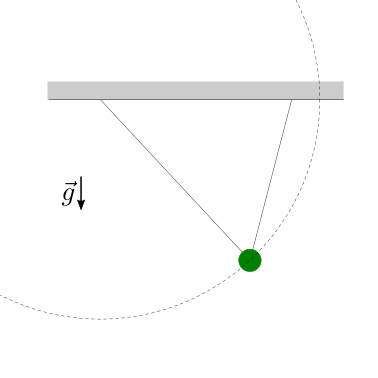
\includegraphics[width=.95\textwidth]{../../media/pb-statics-000-ese-000.png}
\end{minipage}
\end{split}
\end{equation*}
\sphinxAtStartPar
\sphinxstylestrong{Soluzione.}
I fili inestensibili senza massa e senza rigidezza flessionale possono solo trasmettere un’azione assiale. Ci si aiuta qui con un sistema di coordinate cartesiane con asse \(x\) orizzontale con coordinata crescente verso destra e asse \(y\) verticale con coordinata crescente verso l’alto. Date le direzioni dei fili identificate dai vettori unitari \(\hat{t}_1\), \(\hat{t}_2\), l’equilibrio della massa \(m\) è garantito dall’equilibrio delle forze,
\begin{equation*}
\begin{split}\hat{0} = -m g \hat{y} + F_1 \hat{t}_1 + F_2 \hat{t}_2 \ .\end{split}
\end{equation*}
\sphinxAtStartPar
Definiti gli angoli \(\theta_1\), \(\theta_2\), calcolabili dalla geometria del problema \sphinxhyphen{} qui considerati noti e calcolati in seguito \sphinxhyphen{} e tali che \(\hat{t}_1 = \hat{x} \cos \theta_1 + \hat{y}  \sin \theta_1\), \(\hat{t}_2 = \hat{x} \cos \theta_2 + \hat{y} \sin \theta_2\), le componenti cartesiane della condizione di equilibrio forniscono un sistema di due equazioni nelle due incognite \(F_1\), \(F_2\),
\begin{equation*}
\begin{split}\begin{cases} 
  F_1 \cos \theta_1 + F_2 \cos \theta_2 = 0 \\
  F_1 \sin \theta_1 + F_2 \sin \theta_2 = m g \\
\end{cases}\end{split}
\end{equation*}
\sphinxAtStartPar
che ha soluzione
\begin{equation*}
\begin{split}
  \begin{bmatrix} F_1 \\ F_2 \end{bmatrix} 
    = \frac{1}{\cos \theta_1 \sin \theta_2 - \sin \theta_1 \cos \theta_2}
    \begin{bmatrix} \sin \theta_2 & - \cos \theta_2 \\ -\sin \theta_1 & \cos \theta_1 \end{bmatrix} \begin{bmatrix} 0 \\ m g \end{bmatrix} 
    = \frac{1}{\sin(\theta_2 - \theta_1)} \begin{bmatrix} - \cos \theta_2 \\ \cos \theta_1 \end{bmatrix} m g  \ .
\end{split}
\end{equation*}
\sphinxAtStartPar
\sphinxstylestrong{todo} \sphinxstyleemphasis{Controllare conti. Aggiungere immagine.}

\sphinxAtStartPar
\sphinxstylestrong{Grandezze geometriche del problema.} \sphinxstylestrong{todo}
\begin{equation*}
\begin{split}
\begin{minipage}[t]{.55\textwidth}
  \vspace{0pt}
  \textbf{Problema 2.}
  Data la massa $m$ della massa puntiforme appeso tramite due fili inestensibili ideali di lunghezza $L_1$ nota e $L_2$ variabile, si calcolino le reazioni a terra in funzione della lunghezza del filo $2$.
\end{minipage}
\hspace{.05\textwidth}
\begin{minipage}[t]{.40\textwidth}
  \vspace{0pt}
  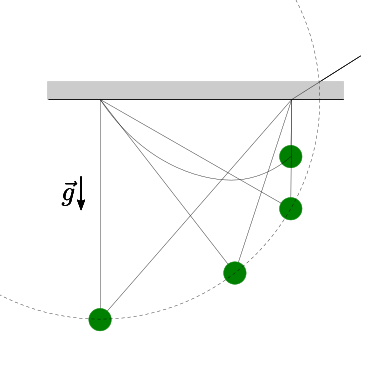
\includegraphics[width=.95\textwidth]{../../media/pb-statics-000-ese-001.png}
\end{minipage}
\end{split}
\end{equation*}
\sphinxAtStartPar
\sphinxstylestrong{Soluzione.}
\begin{equation*}
\begin{split}
\begin{minipage}[t]{.55\textwidth}
  \vspace{0pt}
  \textbf{Problema 3.}
  Data la massa $m$ della massa puntiforme appeso tramite un filo inestensibile ideale di lunghezza $L$ e una molla di costante elastica $k$ e lunghezza a riposo $x_0$ collegata a terra in un punto distante $H$ dal punto a terra dove è collegato il filo, si calcoli:
  \begin{enumerate}
    \item la posizione del punto 
    \item la lunghezza della molla
    \item le reazioni vincolari a terra 
  \end{enumerate}
  nella configurazione di equilibrio.
\end{minipage}
\hspace{.05\textwidth}
\begin{minipage}[t]{.40\textwidth}
  \vspace{0pt}
  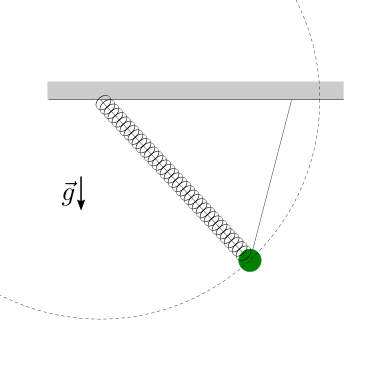
\includegraphics[width=.95\textwidth]{../../media/pb-statics-000-ese-002.png}
\end{minipage}
\end{split}
\end{equation*}
\sphinxAtStartPar
\sphinxstylestrong{Soluzione.}
\begin{equation*}
\begin{split}
\begin{minipage}[t]{.55\textwidth}
  \vspace{0pt}
  \textbf{Problema 4.}
  Data $m$, $\mu^s$, trovare l'angolo massimo $\theta_{\max}$ per il quale esiste una condizione di equilibrio per il cubetto rosso.
\end{minipage}
\hspace{.05\textwidth}
\begin{minipage}[t]{.40\textwidth}
  \vspace{0pt}
  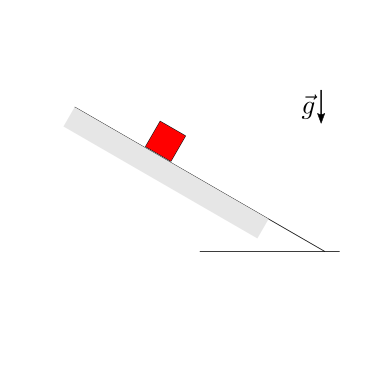
\includegraphics[width=.95\textwidth]{../../media/pb-statics-001-ese-000.png}
\end{minipage}
\end{split}
\end{equation*}
\sphinxAtStartPar
\sphinxstylestrong{Soluzione.}
Per l’equilibrio del corpo è necessario l’equilibrio delle forze. Le forze agenti sul cubetto rosso sono la sua forza peso e la reazione di contatto \(\vec{R}\) con la parete inclinata, che può essere scomposta nella direzione perpendicolare \sphinxhyphen{} reazione normale \sphinxhyphen{} e parallela alla parete \sphinxhyphen{} attrito.

\sphinxAtStartPar
La condizione di equilibrio,
\begin{equation*}
\begin{split}\vec{0} = -m g \hat{y} + \vec{R}\ ,\end{split}
\end{equation*}
\sphinxAtStartPar
può essere proiettata lungo la direzione normale alla parete \(\hat{n}\) e la direzione tangente \(\hat{t}\) (verto l’alto, così che \(\hat{y} = - \cos \theta \, \hat{n} - \sin \theta \, \hat{t}\)
\begin{equation*}
\begin{split}\begin{cases}
0 = N - m g \cos \theta \\
0 = F - m g \sin \theta \ ,
\end{cases}\end{split}
\end{equation*}
\sphinxAtStartPar
così che \(F = N \, \tan \theta\). Bisogna infine verificare che questa forza di attrito statico possa essere trasmessa, con la condizione
\begin{equation*}
\begin{split}|F| \le F^{s,max} = \mu^s \, N \ ,\end{split}
\end{equation*}
\sphinxAtStartPar
insieme alla condizione di contatto \(N \ge 0\), e quindi
\begin{equation*}
\begin{split}|\tan \theta| \le \mu^s \ .\end{split}
\end{equation*}\begin{equation*}
\begin{split}
\begin{minipage}[t]{.55\textwidth}
  \vspace{0pt}
  \textbf{Problema 5.}
  Data $m$, $M$, $\mu^s$ tra i due solidi, si chiede di calcolare:
  \begin{enumerate}
    \item la risultante delle azioni scambiate tra i due corpi
    \item la risultante delle reazioni vincolari a terra agenti sul solido blu,
  \end{enumerate}
  nella condizione di equilibrio del sistema, nell'ipotesi che l'attrito tra solido blu e terra sia trascurabile. Verificare le condizioni limite tra $\theta$ e $\mu^s$ affinché l'equilibrio sia possibile
\end{minipage}
\hspace{.05\textwidth}
\begin{minipage}[t]{.40\textwidth}
  \vspace{0pt}
  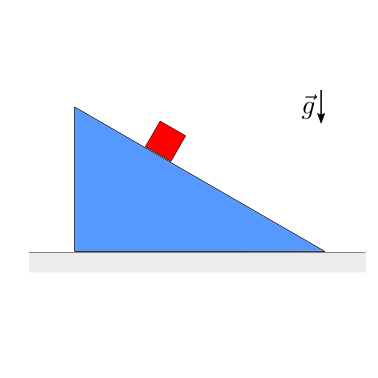
\includegraphics[width=.95\textwidth]{../../media/pb-statics-001-ese-001.png}
\end{minipage}
\end{split}
\end{equation*}
\sphinxAtStartPar
\sphinxstylestrong{Soluzione.}
Il piano orizzontale liscio non può trasmettere nessuna forza orizzontale al prisma triangolare. L’equilibrio delle forze del prisma triangolare, necessaria alla condizione di equilibrio, implica quindi che la risultante delle forze di contatto con il blocchetto rosso ha direzione verticale anch’essa.

\sphinxAtStartPar
Dalla condizione di equilibrio per il blocchetto rosso,
\begin{equation*}
\begin{split}\vec{0} = - m g \hat{y} + \vec{R}_{quad, tri} \qquad \rightarrow \qquad \vec{R}_{quad, tri} = m g \hat{y} \ .\end{split}
\end{equation*}
\sphinxAtStartPar
La risultante delle forze scambiate tra i corpi è quindi uguale e contraria al peso del cubetto (\sphinxstylestrong{1}). L’equilibrio del corpo triangolare
\begin{equation*}
\begin{split}
  \vec{0} = - M g \hat{y} + \vec{R}_{tri, quad} + \vec{R}_{tri, plane} \ ,
\end{split}
\end{equation*}
\sphinxAtStartPar
implica che la reazione \(\vec{R}_{tri,plane}\) agente sul solido triangolare dovuta alla superficie orizzontale è uguale e contraria alla somma del peso dei due solidi (\sphinxstylestrong{2}),
\begin{equation*}
\begin{split}
  \vec{R}_{tri,plane}   = M g \hat{y} - \vec{R}_{tri, quad}     
                        = M g \hat{y} + \vec{R}_{quad, tri}     
                        = M g \hat{y} + m g \hat{y} \ .
\end{split}
\end{equation*}\begin{equation*}
\begin{split}
\begin{minipage}[t]{.55\textwidth}
  \vspace{0pt}
  \textbf{Problema 6.}
  Data la massa $m$ del blocco rosso, la costante elastica $k$ della molla lineare ideale, con lunghezza a riposo $\ell_0$, viene chiesto di:
  \begin{enumerate}
    \item determinare la lunghezza della molla nella condizione di equilibrio, nell'ipotesi che l'attrito tra blocco rosso e piano inclinato sia trascurabile
    \item determinare le possibili condizioni di equilibrio, nell'ipotesi che l'attrito statico tra blocco rosso e piano inclinato sia $\mu^s$
  \end{enumerate}
\end{minipage}
\hspace{.05\textwidth}
\begin{minipage}[t]{.40\textwidth}
  \vspace{0pt}
  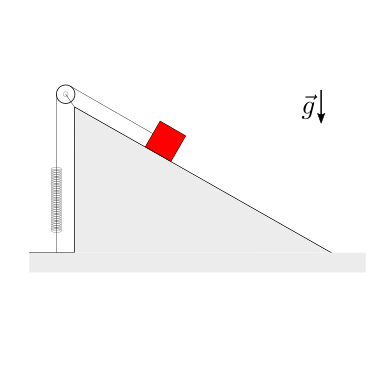
\includegraphics[width=.95\textwidth]{../../media/pb-statics-001-ese-002.png}
\end{minipage}
\end{split}
\end{equation*}
\sphinxAtStartPar
\sphinxstylestrong{Soluzione.}
I fili inestensibili trasmettono solo azione assiale nela direzione del filo, costante in ogni sua sezione. Le condizioni di equilibrio alla rotazione di una carrucola assicurano che sia costante l’azione assiale ai due capi di un filo parzialmente avvolto attorno alla carrucola, nel caso di attriti nulli (carrucola ideale).

\sphinxAtStartPar
Il problema può essere risolto scrivendo le condiizoni di equilibrio della molla,
\begin{equation*}
\begin{split}F = k (\ell - \ell_0)\end{split}
\end{equation*}
\sphinxAtStartPar
e del blocchetto rosso, proiettate in direzione perpendicolare e tangente alla superficie inclinata
\begin{equation*}
\begin{split}
  \vec{0} = \vec{F} + m \vec{g} + \vec{R}
  \qquad , \qquad
  \begin{cases}
    t: \ 0 = - F + m g \sin \theta + F_t \\
    n: \ 0 = \ \ - m g \cos \theta + F_n \\
  \end{cases}
  \end{split}
\end{equation*}
\sphinxAtStartPar
\sphinxstylestrong{In assenza di attrito, \(F_t = 0\).} In assenza di attrito, la reazione tangenziale è nulla \(F_t = 0\) e quindi
\begin{equation*}
\begin{split}\begin{aligned}
  F_n          & = m g \cos \theta \\
  F            & = m g \sin \theta \\
  \Delta \ell  & = \frac{m g}{k} \sin \theta \\
\end{aligned}\end{split}
\end{equation*}
\sphinxAtStartPar
\sphinxstylestrong{Con attrito statico.} In presenza di attrito statico, la soluzione non è unicamente determinata ma bisogna discutere le condizioni che garantiscono l’equilibrio, verificando la condizione \(|F_t| \le \mu^s F_n\). Le espressione delle componenti normali e tangenziali della reazione vincolare agente sul blocchetto,
\begin{equation*}
\begin{split}\begin{aligned}
  F_n & = m g \cos \theta \\
  F_t & = k \Delta \ell - m g \sin \theta
\end{aligned}\end{split}
\end{equation*}
\sphinxAtStartPar
permettono di scrivere la condizione che garantisce l’equilibrio come
\begin{equation*}
\begin{split}
 | k \Delta \ell - m g \sin \theta | \le \mu_s m g \cos \theta 
\end{split}
\end{equation*}
\sphinxAtStartPar
e quindi
\begin{equation*}
\begin{split}- \mu_s m g \cos \theta + mg \sin \theta \le k \Delta \ell \le  \mu_s m g \cos \theta + mg \sin \theta \ .\end{split}
\end{equation*}\begin{equation*}
\begin{split}
\begin{minipage}[t]{.55\textwidth}
  \vspace{0pt}
  \textbf{Problema 7.}
  Data la massa $m$ del blocco rosso, il raggio $R_1$, $R_2$ delle due carrucole, si chiede di determinare la forza $\vec{F}$ da applicare nella condizione di equilibrio, nell'ipotesi di fili inestensibili e carrucole ideali e senza massa.
  % 
  Si chiede poi di ripetere il calcolo nell'ipotesi in cui la massa delle carrucole non sia trascurabile, ma siano $M_1$ per la carrucola vincolata a terra, e $M_2$ per la carrucola non vincolata a terra.
\end{minipage}
\hspace{.05\textwidth}
\begin{minipage}[t]{.40\textwidth}
  \vspace{0pt}
  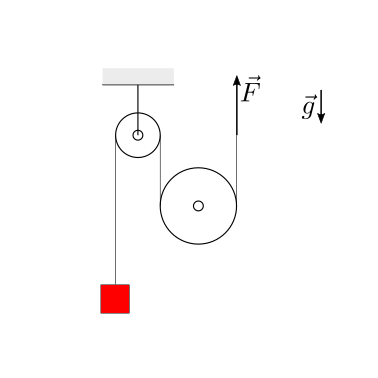
\includegraphics[width=.95\textwidth]{../../media/pb-statics-002-ese-000.png}
\end{minipage}
\end{split}
\end{equation*}
\sphinxAtStartPar
\sphinxstylestrong{Soluzione.}
\begin{equation*}
\begin{split}\begin{aligned}
0 & = - m g + T_1 \\
0 & = F + T_1 - M g \\
0 & - M g R_2 + F \, (2 R_2)
\end{aligned}\end{split}
\end{equation*}\begin{equation*}
\begin{split}\begin{aligned} 
  F & = \frac{1}{2} M g \\
  T_1
\end{aligned}
\end{split}
\end{equation*}\begin{equation*}
\begin{split}
\begin{minipage}[t]{.55\textwidth}
  \vspace{0pt}
  \textbf{Problema 8.}
  Nel meccanismo di un orologio i 3 componenti che devono guidare il moto delle lancette dei secondi, dei minuti e delle ore, connessi "in cascata" tramite ingranaggi (con rapporto dei raggi $1:60$ **todo** scriverlo esplicitamente?). Conoscendo la costante elastica $k$ e la compressione $\Delta \theta$ della molla che guida il componente che guida la lancetta delle ore, si chiede di:
  \begin{enumerate}
    \item determinare la forza necessaria da applicare alla lancetta dei secondi nel punto indicato nell'imagine, necessaria a garantire la posizione di equilibrio
    \item le reazioni vincolari in corrispondenza delle cerniere che collegano a terra i 3 componenti, nell'ipotesi che non si scambino forze in direzione radiale
  \end{enumerate}
\end{minipage}
\hspace{.05\textwidth}
\begin{minipage}[t]{.40\textwidth}
  \vspace{0pt}
  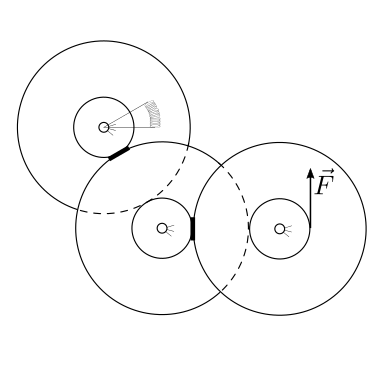
\includegraphics[width=.95\textwidth]{../../media/pb-statics-002-ese-001.png}
\end{minipage}
\end{split}
\end{equation*}
\sphinxAtStartPar
\sphinxstylestrong{Soluzione.}
\begin{equation*}
\begin{split}
F      R_1 & = F_{12} R_2 \\
F_{12} R_2 & = F_{23} R_3 \\
F_{23} R_3 & = k \Delta \theta \ .
\end{split}
\end{equation*}\begin{equation*}
\begin{split}
  F = \frac{R_2}{R_1} \frac{R_3}{R_2} \frac{1}{R_3} k \Delta \theta \ .
\end{split}
\end{equation*}\begin{equation*}
\begin{split}
\begin{minipage}[t]{.55\textwidth}
  \vspace{0pt}
  \textbf{Problema 9.}
  Data la lunghezza $L$ e la massa $m$ dell'asta rigida con distribuzione di massa uniforme e il coefficiente di attrito stativo $\mu^s$ tra asta e superficie orizzontale, si chiede di:
  \begin{enumerate}
    \item determinare la condizione limite dell'equilibrio
    \item determinare le reazioni a terra
  \end{enumerate}
  nell'ipotesi che l'attrito sulla superficie verticale sia trascurabile.
\end{minipage}
\hspace{.05\textwidth}
\begin{minipage}[t]{.40\textwidth}
  \vspace{0pt}
  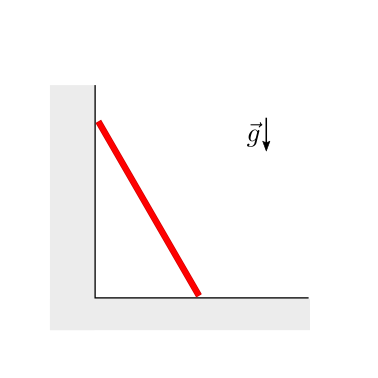
\includegraphics[width=.95\textwidth]{../../media/pb-statics-002-ese-002.png}
\end{minipage}
\end{split}
\end{equation*}
\sphinxAtStartPar
\sphinxstylestrong{Soluzione.}
\begin{equation*}
\begin{split}\begin{aligned}
x & : 0 =  N_{1} + F^{s}_2 \\
y & : 0 = - m g + N_{2} \\
\text{rot, 2} & : 0 = m g \frac{\ell}{2} \cos \theta - N_{1} \ell \sin \theta
\end{aligned}\end{split}
\end{equation*}\begin{equation*}
\begin{split}
\begin{minipage}[t]{.55\textwidth}
  \vspace{0pt}
  \textbf{Problema 10.}
  Data la lunghezza $L$ e la massa $m$ dell'asta rigida incernierata a terra, e la costante elastica $k$ della molla rotazionale, si chiede di:
  \begin{enumerate}
    \item calcolare la condizione di equilibrio
    \item le reazioni vincolari sull'asta
  \end{enumerate}
  discutendo i due casi determinati dalla condizione di appoggio dell'estremo superiore dell'asta sulla parete verticale.
\end{minipage}
\hspace{.05\textwidth}
\begin{minipage}[t]{.40\textwidth}
  \vspace{0pt}
  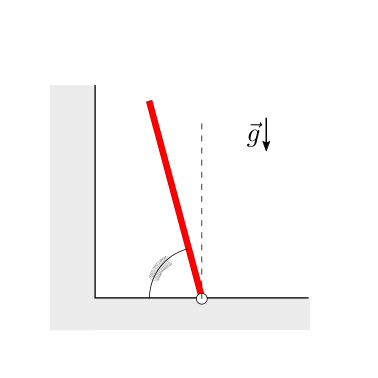
\includegraphics[width=.95\textwidth]{../../media/pb-statics-002-ese-003.png}
\end{minipage}
\end{split}
\end{equation*}
\sphinxAtStartPar
\sphinxstylestrong{Soluzione.}
Nel caso generale,
\begin{equation*}
\begin{split}\begin{aligned}
  x & : 0 =  N_{1} + F_{2,x} \\
  y & : 0 =  - m g + F_{2,y} \\
  \text{rot, 2} & : 0 = m g \frac{\ell}{2} \cos \theta - N_{1} \ell \sin \theta + k \Delta \theta
\end{aligned}\end{split}
\end{equation*}
\sphinxAtStartPar
Il contatto avviene quando la rigidezza della molla garantisce una condizione di equilibrio con \(\Delta \theta < \overline{\Delta \theta}\).
Se non c’è contatto, \(N_1 = 0\); se c’è contatto, in generale \(N_1 > 0\).
\begin{equation*}
\begin{split}
\begin{minipage}[t]{.55\textwidth}
  \vspace{0pt}
  \textbf{Problema 11.}
\end{minipage}
\hspace{.05\textwidth}
\begin{minipage}[t]{.40\textwidth}
  \vspace{0pt}
  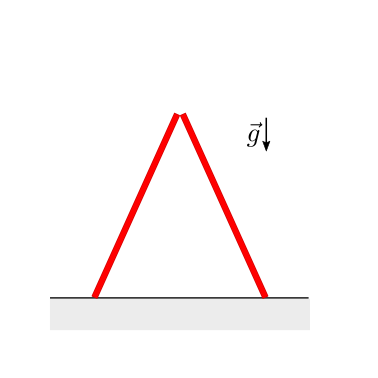
\includegraphics[width=.95\textwidth]{../../media/pb-statics-002-ese-004.png}
\end{minipage}
\end{split}
\end{equation*}
\sphinxAtStartPar
\sphinxstylestrong{Soluzione.}
\begin{equation*}
\begin{split}
\begin{minipage}[t]{.55\textwidth}
  \vspace{0pt}
  \textbf{Problema 12.}
\end{minipage}
\hspace{.05\textwidth}
\begin{minipage}[t]{.40\textwidth}
  \vspace{0pt}
  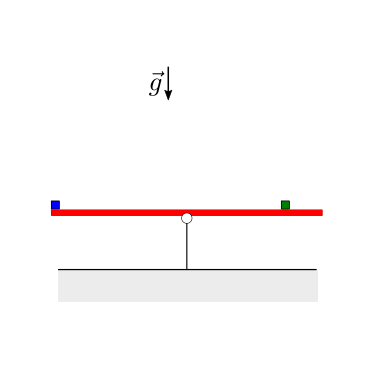
\includegraphics[width=.95\textwidth]{../../media/pb-statics-002-ese-005.png}
\end{minipage}
\end{split}
\end{equation*}
\sphinxAtStartPar
\sphinxstylestrong{Soluzione.}
\begin{equation*}
\begin{split}
\begin{minipage}[t]{.55\textwidth}
  \vspace{0pt}
  \textbf{Problema 13.}
\end{minipage}
\hspace{.05\textwidth}
\begin{minipage}[t]{.40\textwidth}
  \vspace{0pt}
  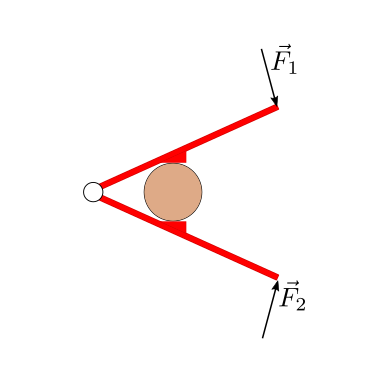
\includegraphics[width=.95\textwidth]{../../media/pb-statics-002-ese-006.png}
\end{minipage}
\end{split}
\end{equation*}
\sphinxAtStartPar
\sphinxstylestrong{Soluzione.}
\begin{equation*}
\begin{split}
\begin{minipage}[t]{.55\textwidth}
  \vspace{0pt}
  \textbf{Problema 14.}
\end{minipage}
\hspace{.05\textwidth}
\begin{minipage}[t]{.40\textwidth}
  \vspace{0pt}
  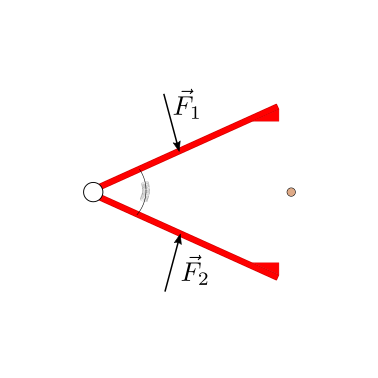
\includegraphics[width=.95\textwidth]{../../media/pb-statics-002-ese-007.png}
\end{minipage}
\end{split}
\end{equation*}
\sphinxAtStartPar
\sphinxstylestrong{Soluzione.}
\begin{equation*}
\begin{split}
\begin{minipage}[t]{.55\textwidth}
  \vspace{0pt}
  \textbf{Problema 15.}
  Equilibrio di un corpo appoggiato...esempio che mostra come la retta di applicazione del peso deve cadere nella base di appoggio; qui non è possibile introdurre l'accelerazione del sistema (**todo** *aggiungere esercizio nel capitolo della dinamica*), ma si può fare un esercizio con superficie di appoggio permendicolare e non al campo di gravità locale. L'unica cosa che conta è la direzione relativa tra superficie di appoggio e forza di massa. Rimandare all'esercizio sulla dinamica con collegamento
\end{minipage}
\hspace{.05\textwidth}
\begin{minipage}[t]{.40\textwidth}
\end{minipage}
\end{split}
\end{equation*}
\sphinxAtStartPar
\sphinxstylestrong{Soluzione.}
\begin{equation*}
\begin{split}
\begin{minipage}[t]{.55\textwidth}
  \vspace{0pt}
  \textbf{Problema 16.}
  Sollevamento di un peso sbilanciato, come mostrato in un *"video virale"*
\end{minipage}
\hspace{.05\textwidth}
\begin{minipage}[t]{.40\textwidth}
\end{minipage}
\end{split}
\end{equation*}
\sphinxAtStartPar
\sphinxstylestrong{Soluzione.}

\sphinxstepscope




\chapter{Inerzia}
\label{\detokenize{ch/mechanics/inertia:inerzia}}\label{\detokenize{ch/mechanics/inertia:physics-hs-mechanics-inertia}}\label{\detokenize{ch/mechanics/inertia::doc}}
\sphinxAtStartPar
L’inerzia di un sistema meccanico rappresenta una misura della sua resistenza al cambiamento dello stato di moto, in seguito all’applicazione di forze esterne sul sistema: la combinazione delle proprietà inerziali di un sistema con le grandezze cinematiche che ne caratterizzano il moto produce infatti le \DUrole{xref,myst}{quantità dinamiche}, la cui variazione nel tempo è legata all’azione delle azioni esterne sul sistema dai principi della dinamica e dalle equazioni di moto che governano la dinamica dei sistemi.
Le proprietà inerziali di un corpo dipendono dalla sua massa e dalla distribuzione nello spazio della sua massa.

\sphinxAtStartPar
\sphinxstylestrong{Ma cos’è la massa?}%
\begin{footnote}[1]\sphinxAtStartFootnote
La risposta alla domanda «cos’è la massa?» potrebbe implicare una conoscenza «vera» \sphinxhyphen{} qualsiasi cosa significhi \sphinxhyphen{} del concetto di «massa». Anche qui, come già in altre parti, la domanda «cos’è…?» può essere sostituita con «cosa intendiamo per…?», e una «risposta operativa» può essere ritenuta soddisfacente, poiché rispecchia la modalità di conoscenza e formazione del sapere in ambito scientifico: senza entrare in ambiti filosofici più astratti, in fisica siamo contenti di definire qualcosa tramite le sue interazioni ed effetti su altri sistemi, le sue proprietà, e un processo affidabile per la sua misura.
%
\end{footnote} la massa è una grandezza fisica che rappresenta la quantità di materia e si manifesta:
\begin{itemize}
\item {} 
\sphinxAtStartPar
tramite la sua {\hyperref[\detokenize{ch/mechanics/actions-examples:physics-hs-mechanics-actions-gravitation}]{\sphinxcrossref{\DUrole{std,std-ref}{interazione gravitazionale}}}} con altri corpi dotati di massa;

\item {} 
\sphinxAtStartPar
come una misura della resistenza di un sistema ai cambiamenti del suo stato di moto in risposta a una forza applicata, come sarà chiaro dalle equazioni della {\hyperref[\detokenize{ch/mechanics/dynamics:physics-hs-mechanics-dynamics}]{\sphinxcrossref{\DUrole{std,std-ref}{dinamica}}}}

\end{itemize}
\label{ch/mechanics/inertia:example-0}
\begin{sphinxadmonition}{note}{Example 11.1 (Massa gravitazionale e massa inerziale)}



\sphinxAtStartPar
Le due manifestazioni diverse della massa possono essere usate come definizione di due grandezze diverse: l’interazione gravitazionale di un sistema con altri corpi dotati di massa può essere usata per definire la \sphinxstylestrong{massa gravitazionale} del sistema; il cambio di moto dello stesso sistema quando soggetto ad azioni esterne può essere usato per definirne la \sphinxstylestrong{massa inerziale}. L’evidenza sperimentale dimostra che le due grandezze fisiche così definite sono omogenee e producono lo stessa misura: si può pensare ai due procedimenti come due metodi di misura differenti della stessa grandezza fisica, che usano due interazioni differenti della massa con altri oggetti fisici.
\end{sphinxadmonition}

\sphinxAtStartPar
Dal punto di vista operativo, la massa di un sistema \sphinxhyphen{} quando possibile dal punto di vista pratico \sphinxhyphen{} può essere misurata tramite la sua interazione con un campo di gravitazione noto, tramite una \sphinxstylestrong{bilancia}



\sphinxAtStartPar
\sphinxstylestrong{Distribuzione di massa.}



\sphinxAtStartPar
\sphinxstylestrong{Quantità dinamiche.}
Come sarà chiaro nello sviluppo delle {\hyperref[\detokenize{ch/mechanics/dynamics-notes:physics-hs-mechanics-dynamics-eom-points}]{\sphinxcrossref{\DUrole{std,std-ref}{equazioni di moto di un sistema}}}}, la definizione di alcune grandezze dinamiche additive risulta naturale, fornendo dei concetti utili e sintetici per la costruzione di un modello e l’interpretazione dei fenomeni fisici.

\sphinxAtStartPar
Queste grandezze dinamiche combinano la massa e la sua distribuzione con le grandezze cinematiche del sistema. In particolare, risulta utile definire tre grandezze:
\begin{itemize}
\item {} 
\sphinxAtStartPar
quantità di moto

\item {} 
\sphinxAtStartPar
momento della quantità di moto

\item {} 
\sphinxAtStartPar
energia cinetica

\end{itemize}

\sphinxAtStartPar
Le {\hyperref[\detokenize{ch/mechanics/dynamics-eom:physics-hs-mechanics-dynamics-eom}]{\sphinxcrossref{\DUrole{std,std-ref}{equazioni del moto}}}} dei sistemi rappresentano delle equazioni differenziali che mettono in relazione la variazione di queste quantità dinamiche con la causa di queste variazioni, in generale riconducibile ad {\hyperref[\detokenize{ch/mechanics/actions:physics-hs-mechanics-actions}]{\sphinxcrossref{\DUrole{std,std-ref}{azioni}}}} agenti sul sistema.
Sotto opportune ipotesi, queste grandezze dinamiche sono costanti del moto, come descritto dalle {\hyperref[\detokenize{ch/mechanics/dynamics-conservation:physics-hs-mechanics-dynamics-conservation}]{\sphinxcrossref{\DUrole{std,std-ref}{leggi di conservazione}}}}.

\sphinxAtStartPar
Le 3 grandezze dinamiche possono avere espressioni diverse, a seconda del sistema di interesse. Nel caso di corpi rigidi, queste possono essere espresse in termini di velocità di un punto materiale e della velocità angolare del corpo.


\bigskip\hrule\bigskip


\sphinxstepscope




\section{Inerzia e grandezze dinamiche di un punto}
\label{\detokenize{ch/mechanics/inertia-point:inerzia-e-grandezze-dinamiche-di-un-punto}}\label{\detokenize{ch/mechanics/inertia-point:physics-hs-mechanics-inertia-point}}\label{\detokenize{ch/mechanics/inertia-point::doc}}

\subsection{Inerzia}
\label{\detokenize{ch/mechanics/inertia-point:inerzia}}\label{\detokenize{ch/mechanics/inertia-point:physics-hs-mechanics-inertia-point-inertia}}

\subsection{Grandezze dinamiche}
\label{\detokenize{ch/mechanics/inertia-point:grandezze-dinamiche}}\label{\detokenize{ch/mechanics/inertia-point:physics-hs-mechanics-inertia-point-dynamical-quantities}}\begin{equation*}
\begin{split}\begin{aligned}
  \vec{Q}_P     & = m_P \, \vec{v}_P \\
  \vec{L}_{P,H} & = m_P \, (P - H) \times \vec{v}_P \\
   K_P          & = \frac{1}{2} m_P \left| \vec{v}_P \right|^2
\end{aligned}\end{split}
\end{equation*}
\sphinxstepscope




\section{Inerzia e grandezze dinamiche di un sistema esteso con distribuzione discreta di massa}
\label{\detokenize{ch/mechanics/inertia-points:inerzia-e-grandezze-dinamiche-di-un-sistema-esteso-con-distribuzione-discreta-di-massa}}\label{\detokenize{ch/mechanics/inertia-points:physics-hs-mechanics-inertia-points}}\label{\detokenize{ch/mechanics/inertia-points::doc}}

\subsection{Inerzia}
\label{\detokenize{ch/mechanics/inertia-points:inerzia}}\label{\detokenize{ch/mechanics/inertia-points:physics-hs-mechanics-inertia-points-inertia}}

\subsection{Grandezze dinamiche}
\label{\detokenize{ch/mechanics/inertia-points:grandezze-dinamiche}}\label{\detokenize{ch/mechanics/inertia-points:physics-hs-mechanics-inertia-points-dynamical-quantities}}\begin{equation*}
\begin{split}\begin{aligned}
  \vec{Q}       = \sum_i \vec{Q}_i     & = \sum_i  m_i \, \vec{v}_i \\
  \vec{L}_{H}   = \sum_i \vec{L}_{i,H} & = \sum_i  m_i \, (P_i - H) \times \vec{v}_i \\
   K            = \sum_i  K_i          & = \sum_i  \frac{1}{2} m_i \left| \vec{v}_i \right|^2
\end{aligned}\end{split}
\end{equation*}

\subsection{Sistemi rigidi}
\label{\detokenize{ch/mechanics/inertia-points:sistemi-rigidi}}
\sphinxAtStartPar
Usando la definizione di centro di massa
\begin{equation*}
\begin{split}m G = \sum_i m_i P_i\end{split}
\end{equation*}
\sphinxAtStartPar
e legge del moto rigido
\begin{equation*}
\begin{split}\vec{v}_i - \vec{v}_P = \vec{\omega} \times (P_i - P)\end{split}
\end{equation*}
\sphinxAtStartPar
le quantità dinamiche possono essere espresse in funzione della velocità del punto di riferimento \(P\) e della velocità angolare del sistema, tramite la massa e le altre quantità inerziali
\begin{itemize}
\item {} 
\sphinxAtStartPar
la quantità di moto

\end{itemize}
\begin{equation*}
\begin{split}\begin{aligned}
  \vec{Q} = \sum_i m_i \vec{v}_i
        & = \sum_i m_i \left( \vec{v}_P + \vec{\omega} \times (P_i - P) \right) = \\
        & =  m \vec{v}_P + \vec{\omega} \times m (G - P) 
\end{aligned}\end{split}
\end{equation*}\begin{itemize}
\item {} 
\sphinxAtStartPar
momento della quantità di moto

\end{itemize}
\begin{equation*}
\begin{split}\begin{aligned}
  \vec{L}_H = \sum_i m_i (P_i - H) \times \vec{v}_i
        & = \sum_i m_i \left( P_i - P + \vec{r}_P - \vec{r}_H \right) \times \vec{v}_i = \\
        & = \sum_i m_i \left( P_i - P \right) \times \vec{v}_i + \left( P - H \right) \times \vec{Q}  = \\
        & = \sum_i m_i \left( P_i - P \right) \times \left( \vec{v}_P - \left( P_i - P \right) \times \vec{\omega} \right) + \left( P - H \right) \times \vec{Q}  = \\
        & = m (G - P) \times \vec{v}_P - \sum_i m_i \left( P_i - P \right) \times \left( \left( P_i - P \right) \times \vec{\omega} \right) + \left( P - H \right) \times \vec{Q}  = \\
        & = \mathbb{I}_P \cdot \vec{\omega} +  m (G - P) \times \vec{v}_P + \left( P - H \right) \times \vec{Q}
\end{aligned}\end{split}
\end{equation*}
\sphinxAtStartPar
Nel caso di moto 2\sphinxhyphen{}dimensionale e velocità angolare perpendicolare a questo piano, \sphinxstylestrong{todo}
\begin{equation*}
\begin{split}\begin{aligned}
  \vec{r}_{i/P} & := P_i - P = \left( x_i - x_P \right) \hat{x} + \left( y_i - y_P \right) \hat{y} \\
  \vec{\omega} & = \dot{\theta} \, \hat{z}
\end{aligned}\end{split}
\end{equation*}\begin{equation*}
\begin{split}\begin{aligned}
  - \vec{r}_{i/P} \times \left( \vec{r}_{i/P} \times \hat{\omega} \right) 
  & = - ( \Delta x_i \hat{x} + \Delta y_i \hat{y} ) \times \left[ ( \Delta x_i \hat{x} + \Delta y_i \hat{y} ) \times \dot{\theta} \hat{z} \right] = \\ 
  & = - \dot{\theta} ( \Delta x_i \hat{x} + \Delta y_i \hat{y} ) \times \left( - \Delta x_i \hat{y} + \Delta y_i \hat{x} \right) = \\
  & = \left( \Delta x_i^2 + \Delta y_i^2 \right) \dot{\theta} \, \hat{z} \ .
\end{aligned}\end{split}
\end{equation*}
\sphinxAtStartPar
e l’espressione del momento della quantità di moto diventa
\begin{equation*}
\begin{split}\vec{L}_{H} = I_P \, \vec{\omega} +  m (G - P) \times \vec{v}_P + \left( P - H \right) \times \vec{Q}\end{split}
\end{equation*}
\sphinxAtStartPar
con
\begin{equation*}
\begin{split}I_P = \sum_i m_i \left[ \left(x_i - x_P\right)^2 + \left(y_i - y_P\right)^2 \right]\end{split}
\end{equation*}
\sphinxstepscope




\section{Inerzia e grandezze dinamiche di un sistema esteso con distribuzione continua di massa}
\label{\detokenize{ch/mechanics/inertia-continuum:inerzia-e-grandezze-dinamiche-di-un-sistema-esteso-con-distribuzione-continua-di-massa}}\label{\detokenize{ch/mechanics/inertia-continuum:physics-hs-mechanics-inertia-continuum}}\label{\detokenize{ch/mechanics/inertia-continuum::doc}}

\subsection{Sistemi rigidi}
\label{\detokenize{ch/mechanics/inertia-continuum:sistemi-rigidi}}\label{\detokenize{ch/mechanics/inertia-continuum:physics-hs-mechanics-inertia-continuum-rigid}}\label{ch/mechanics/inertia-continuum:inertia-sphere}
\begin{sphinxadmonition}{note}{Example 11.3.1 (Inerzia di una sfera)}



\sphinxAtStartPar
Una sfera di massa \(m\) ha inerzia alla rotazione

\sphinxAtStartPar
usando le coordinate cilindriche
\begin{equation*}
\begin{split}I = \int_V \rho \dots = \frac{2}{5} m R^2 \ . \end{split}
\end{equation*}
\sphinxAtStartPar
usando le coordinate sferiche
\begin{equation*}
\begin{split}I = \int_V \rho \dots = \frac{2}{5} m R^2 \ . \end{split}
\end{equation*}
\sphinxAtStartPar
con la massa
\begin{equation*}
\begin{split}m = \dots = \frac{4}{3} \pi \rho R^3 \ ,\end{split}
\end{equation*}\end{sphinxadmonition}
\label{ch/mechanics/inertia-continuum:inertia-sphere-non-uniform}
\begin{sphinxadmonition}{note}{Example 11.3.2 (Inerzia di una sfera con distribuzione di massa non uniforme)}


\end{sphinxadmonition}
\label{ch/mechanics/inertia-continuum:inertia-disk}
\begin{sphinxadmonition}{note}{Example 11.3.3 (Inerzia di un disco uniforme)}



\sphinxAtStartPar
Un disco di massa \(m\) ha inerzia alla rotazione
\begin{equation*}
\begin{split}I = \int_S \sigma \left( x^2 + y^2 \right) = \int_{\theta=0}^{2\pi} \int_{r=0}^{R} \sigma r^2 \, r \, dr \, d\theta = 2 \pi \sigma \frac{R^4}{4} = \frac{1}{2} \pi \sigma R^4 = \frac{1}{2} m R^2 \ . \end{split}
\end{equation*}\begin{equation*}
\begin{split}m = \int_S \sigma = \int_{\theta = 0}^{2 \pi} \int_{r=0}^{R} \sigma \, r \, dr \, d\theta = 2 \pi \sigma \frac{R^2}{2} = \pi \sigma R^2 \ ,\end{split}
\end{equation*}\begin{equation*}
\begin{split}\sigma = \frac{m}{\pi R^2} \ .\end{split}
\end{equation*}\end{sphinxadmonition}
\label{ch/mechanics/inertia-continuum:inertia-disk-non-uniform-non-symmetric}
\begin{sphinxadmonition}{note}{Example 11.3.4 (Inerzia di un disco uniforme)}


\end{sphinxadmonition}
\label{ch/mechanics/inertia-continuum:inertia-ring}
\begin{sphinxadmonition}{note}{Example 11.3.5 (Inerzia di un anello uniforme)}



\sphinxAtStartPar
Un anello di massa \(m\) ha inerzia alla rotazione
\begin{equation*}
\begin{split}I = \oint_C \mu \left( x^2 + y^2 \right) = \int_{\theta=0}^{2\pi}  \mu R^2 \, R \, d\theta = 2 \pi \mu R^3 = m R^2 \ . \end{split}
\end{equation*}\begin{equation*}
\begin{split}m = \oint_C \mu = \int_{\theta = 0}^{2 \pi} \mu \, R \, d\theta = 2 \pi \mu R \end{split}
\end{equation*}\begin{equation*}
\begin{split}\mu = \frac{m}{2 \pi R} \ .\end{split}
\end{equation*}\end{sphinxadmonition}

\sphinxstepscope


\section{Problemi}
\label{\detokenize{ch/mechanics/inertia-problems:problemi}}\label{\detokenize{ch/mechanics/inertia-problems::doc}}
\sphinxAtStartPar
Questa pagina contiene esercizi sull’inerzia dei sistemi meccanici, con valutazione dell’impulso, del momento angolare, dell’energia cinetica, e del tensore di inerzia. Gli esercizi riguardano punti materiali, sistemi di punti materiali e distribuzioni di massa continua, con applicazioni del teorema del trasporto di Huygens in alcuni casi.


\bigskip\hrule\bigskip



\subsection{Punti Materiali}
\label{\detokenize{ch/mechanics/inertia-problems:punti-materiali}}\phantomsection \label{exercise:ch/mechanics/inertia-problems-exercise-0}

\begin{sphinxadmonition}{note}{Exercise 11.4.1 (Momento di Inerzia di un Punto)}



\sphinxAtStartPar
Un punto materiale di massa \(m = 5 \, \text{kg}\) si trova a una distanza \(r = 3 \, \text{m}\) da un asse di rotazione. Calcola il momento di inerzia di questo punto rispetto a tale asse.
\end{sphinxadmonition}
\phantomsection \label{exercise:ch/mechanics/inertia-problems-exercise-1}

\begin{sphinxadmonition}{note}{Exercise 11.4.2 (Energia Cinetica di un Punto in Rotazione)}



\sphinxAtStartPar
Un punto materiale di massa \(m = 5 \, \text{kg}\) è in rotazione attorno a un asse con velocità angolare \(\omega = 4 \, \text{rad/s}\). Calcola la sua energia cinetica rotazionale.
\end{sphinxadmonition}
\phantomsection \label{exercise:ch/mechanics/inertia-problems-exercise-2}

\begin{sphinxadmonition}{note}{Exercise 11.4.3 (Impulso e Momento Angolare di un Punto)}



\sphinxAtStartPar
Un punto materiale di massa \(m = 3 \, \text{kg}\) si muove lungo una traiettoria circolare di raggio \(r = 2 \, \text{m}\) con velocità lineare \(v = 6 \, \text{m/s}\). Calcola l’impulso e il momento angolare rispetto al centro della traiettoria.
\end{sphinxadmonition}
\phantomsection \label{exercise:ch/mechanics/inertia-problems-exercise-3}

\begin{sphinxadmonition}{note}{Exercise 11.4.4 (Legge di Conservazione del Momento Angolare)}



\sphinxAtStartPar
Un corpo di massa \(m = 2 \, \text{kg}\) ruota con velocità angolare \(\omega_1 = 5 \, \text{rad/s}\) e raggio \(r = 1 \, \text{m}\). Successivamente, il corpo subisce una variazione di massa che porta a \(m = 4 \, \text{kg}\), mantenendo costante la sua velocità angolare. Calcola il nuovo momento angolare.
\end{sphinxadmonition}
\phantomsection \label{exercise:ch/mechanics/inertia-problems-exercise-4}

\begin{sphinxadmonition}{note}{Exercise 11.4.5 (Energia Cinetica e Momento Angolare)}



\sphinxAtStartPar
Un punto materiale di massa \(m = 2 \, \text{kg}\) ruota attorno a un asse con velocità angolare \(\omega = 6 \, \text{rad/s}\) a una distanza \(r = 4 \, \text{m}\). Calcola l’energia cinetica e il momento angolare.
\end{sphinxadmonition}


\bigskip\hrule\bigskip



\subsection{Sistemi di Punti Materiali}
\label{\detokenize{ch/mechanics/inertia-problems:sistemi-di-punti-materiali}}\phantomsection \label{exercise:ch/mechanics/inertia-problems-exercise-5}

\begin{sphinxadmonition}{note}{Exercise 11.4.6 (Momento di Inerzia di un Sistema di Punti)}



\sphinxAtStartPar
Tre masse, \(m_1 = 2 \, \text{kg}\), \(m_2 = 3 \, \text{kg}\), e \(m_3 = 4 \, \text{kg}\), sono disposte su un piano cartesiano nelle seguenti posizioni: \((1, 0)\), \((0, 2)\), e \((-1, -1)\). Calcola il momento di inerzia totale del sistema rispetto all’asse \(z\) (perpendicolare al piano).
\end{sphinxadmonition}
\phantomsection \label{exercise:ch/mechanics/inertia-problems-exercise-6}

\begin{sphinxadmonition}{note}{Exercise 11.4.7 (Momento Angolare di un Sistema di Punti)}



\sphinxAtStartPar
Un sistema di tre masse, \(m_1 = 1 \, \text{kg}\), \(m_2 = 2 \, \text{kg}\), e \(m_3 = 3 \, \text{kg}\), si muove su traiettorie circolari di raggi rispettivamente \(r_1 = 2 \, \text{m}\), \(r_2 = 3 \, \text{m}\), e \(r_3 = 4 \, \text{m}\). Se le velocità tangenziali sono \(v_1 = 5 \, \text{m/s}\), \(v_2 = 6 \, \text{m/s}\), e \(v_3 = 7 \, \text{m/s}\), calcola il momento angolare totale del sistema rispetto all’origine.
\end{sphinxadmonition}
\phantomsection \label{exercise:ch/mechanics/inertia-problems-exercise-7}

\begin{sphinxadmonition}{note}{Exercise 11.4.8 (Energia Cinetica di un Sistema di Punti)}



\sphinxAtStartPar
Un sistema di 4 masse, disposte lungo un’asse \(x\), ha masse \(m_1 = 2 \, \text{kg}\), \(m_2 = 3 \, \text{kg}\), \(m_3 = 4 \, \text{kg}\), e \(m_4 = 5 \, \text{kg}\) a distanze rispettivamente di \(r_1 = 1 \, \text{m}\), \(r_2 = 2 \, \text{m}\), \(r_3 = 3 \, \text{m}\), e \(r_4 = 4 \, \text{m}\). Calcola l’energia cinetica totale del sistema, considerando che tutte le masse si muovono con velocità angolare uniforme \(\omega = 3 \, \text{rad/s}\).
\end{sphinxadmonition}
\phantomsection \label{exercise:ch/mechanics/inertia-problems-exercise-8}

\begin{sphinxadmonition}{note}{Exercise 11.4.9 (Momento di Inerzia di un Sistema di Punti in Movimento)}



\sphinxAtStartPar
Un sistema di masse \(m_1 = 3 \, \text{kg}\) e \(m_2 = 4 \, \text{kg}\) si muovono su traiettorie circolari con raggi \(r_1 = 2 \, \text{m}\) e \(r_2 = 3 \, \text{m}\) rispettivamente. Calcola il momento di inerzia del sistema rispetto a un asse passante per l’origine.
\end{sphinxadmonition}
\phantomsection \label{exercise:ch/mechanics/inertia-problems-exercise-9}

\begin{sphinxadmonition}{note}{Exercise 11.4.10 (Teorema del Trasporto di Huygens)}



\sphinxAtStartPar
Un sistema di punti materiali con masse \(m_1 = 2 \, \text{kg}\), \(m_2 = 3 \, \text{kg}\) e \(m_3 = 4 \, \text{kg}\) ruota attorno a un asse con velocità angolare \(\omega = 2 \, \text{rad/s}\). Il sistema si sposta di \(3 \, \text{m}\) lungo l’asse \(x\). Usa il teorema del trasporto di Huygens per calcolare la variazione dell’energia cinetica durante il trasporto.
\end{sphinxadmonition}


\bigskip\hrule\bigskip



\subsection{Sistemi con Distribuzione Continua di Massa}
\label{\detokenize{ch/mechanics/inertia-problems:sistemi-con-distribuzione-continua-di-massa}}\phantomsection \label{exercise:ch/mechanics/inertia-problems-exercise-10}

\begin{sphinxadmonition}{note}{Exercise 11.4.11 (Momento di Inerzia di un Disco)}



\sphinxAtStartPar
Calcola il momento di inerzia di un disco di massa \(m = 10 \, \text{kg}\) e raggio \(R = 5 \, \text{m}\) rispetto all’asse centrale e perpendicolare al piano del disco.
\end{sphinxadmonition}
\phantomsection \label{exercise:ch/mechanics/inertia-problems-exercise-11}

\begin{sphinxadmonition}{note}{Exercise 11.4.12 (Energia Cinetica di un Disco in Rotazione)}



\sphinxAtStartPar
Un disco di massa \(m = 8 \, \text{kg}\) e raggio \(R = 4 \, \text{m}\) ruota con una velocità angolare \(\omega = 6 \, \text{rad/s}\). Calcola la sua energia cinetica totale.
\end{sphinxadmonition}
\phantomsection \label{exercise:ch/mechanics/inertia-problems-exercise-12}

\begin{sphinxadmonition}{note}{Exercise 11.4.13 (Momento Angolare di un Corpo Rigido)}



\sphinxAtStartPar
Un corpo rigido ruota attorno a un asse con velocità angolare \(\omega = 4 \, \text{rad/s}\). Se la massa totale del corpo è \(m = 6 \, \text{kg}\) e il raggio di rotazione medio è \(r = 2 \, \text{m}\), calcola il momento angolare del corpo.
\end{sphinxadmonition}
\phantomsection \label{exercise:ch/mechanics/inertia-problems-exercise-13}

\begin{sphinxadmonition}{note}{Exercise 11.4.14 (Energia Cinetica di un Corpo Rigido in Rotazione e Traslazione)}



\sphinxAtStartPar
Un corpo rigido di massa \(m = 5 \, \text{kg}\) e raggio \(r = 3 \, \text{m}\) si muove in traslazione con velocità \(v = 2 \, \text{m/s}\) e ruota attorno a un asse con velocità angolare \(\omega = 4 \, \text{rad/s}\). Calcola l’energia cinetica totale del corpo.
\end{sphinxadmonition}
\phantomsection \label{exercise:ch/mechanics/inertia-problems-exercise-14}

\begin{sphinxadmonition}{note}{Exercise 11.4.15 (Momento di Inerzia di una Barra)}



\sphinxAtStartPar
Calcola il momento di inerzia di una barra di lunghezza \(L = 2 \, \text{m}\) e massa \(m = 4 \, \text{kg}\) rispetto a un asse che passa per un’estremità e perpendicolare alla barra.
\end{sphinxadmonition}
\phantomsection \label{exercise:ch/mechanics/inertia-problems-exercise-15}

\begin{sphinxadmonition}{note}{Exercise 11.4.16 (Energia Cinetica di una Barra in Rotazione)}



\sphinxAtStartPar
Una barra di massa \(m = 3 \, \text{kg}\) e lunghezza \(L = 2 \, \text{m}\) ruota con velocità angolare \(\omega = 5 \, \text{rad/s}\) attorno a un asse perpendicolare alla barra e situato al suo centro di massa. Calcola l’energia cinetica totale.
\end{sphinxadmonition}
\phantomsection \label{exercise:ch/mechanics/inertia-problems-exercise-16}

\begin{sphinxadmonition}{note}{Exercise 11.4.17 (Momento di Inerzia di un Solido)}



\sphinxAtStartPar
Calcola il momento di inerzia di un cilindro solido di massa \(m = 12 \, \text{kg}\) e raggio \(R = 3 \, \text{m}\) rispetto a un asse che passa attraverso il centro e perpendicolare al piano del cilindro.
\end{sphinxadmonition}
\phantomsection \label{exercise:ch/mechanics/inertia-problems-exercise-17}

\begin{sphinxadmonition}{note}{Exercise 11.4.18 (Teorema del Trasporto di Huygens Applicato a un Solido)}



\sphinxAtStartPar
Un cilindro solido ruota con velocità angolare \(\omega = 4 \, \text{rad/s}\) attorno a un asse passante per il suo centro. Calcola la variazione dell’energia cinetica se il cilindro si sposta lungo l’asse \(x\) di \(2 \, \text{m}\) utilizzando il teorema del trasporto di Huygens.
\end{sphinxadmonition}
\phantomsection \label{exercise:ch/mechanics/inertia-problems-exercise-18}

\begin{sphinxadmonition}{note}{Exercise 11.4.19 (Momento di Inerzia di un Solido Sottile)}



\sphinxAtStartPar
Un oggetto sottile e rigido di massa \(m = 6 \, \text{kg}\) e lunghezza \(L = 3 \, \text{m}\) ha una distribuzione di massa lineare uniforme. Calcola il momento di inerzia rispetto a un asse perpendicolare al piano e situato al centro dell’oggetto.
\end{sphinxadmonition}
\phantomsection \label{exercise:ch/mechanics/inertia-problems-exercise-19}

\begin{sphinxadmonition}{note}{Exercise 11.4.20 (Energia Cinetica di un Corpo Rotante)}



\sphinxAtStartPar
Un corpo rigido di massa \(m = 15 \, \text{kg}\) e momento di inerzia \$I =
\end{sphinxadmonition}

\sphinxstepscope




\chapter{Dinamica}
\label{\detokenize{ch/mechanics/dynamics:dinamica}}\label{\detokenize{ch/mechanics/dynamics:physics-hs-mechanics-dynamics}}\label{\detokenize{ch/mechanics/dynamics::doc}}
\sphinxAtStartPar
La dinamica si occupa del moto dei sistemi e delle cause del moto, mettendo insieme la descrizione cinematica, l’inerzia dei sistemi a perseverare nel moto, e le cause di una variazione del moto.

\sphinxAtStartPar
\sphinxstylestrong{Princìpi della dinamica.} Vengono discussi i tre principi della dinamica di Newton e il significato della relatività galileiana.

\sphinxAtStartPar
\sphinxstylestrong{Equazioni cardinali della dinamica.} Vengono presentate le tre equazioni cardinali della dinamica per sistemi chiusi, che mettono in relazione la variazione delle grandezze dinamiche alle azioni, e che nel caso di moti regolari possono essere scritte in forma differenziale
\begin{equation*}
\begin{split}\begin{aligned}
 \dot{\vec{Q}} & = \vec{R}^{ext} & \text{(bilancio quantità di moto)} \\
 \dot{\vec{L}}_H + \dot{\vec{x}}_H \times \vec{Q} & = \vec{M}_H^{ext} & \text{(bilancio momento della quantità di moto)} \\
 \dot{K} & = P^{tot} & \text{(bilancio energia cinetica)} \ .
\end{aligned}\end{split}
\end{equation*}
\sphinxAtStartPar
Viene dimostrato che le equazioni di bilancio hanno la stessa forma per ogni sistema chiuso se scritti in termini di variazione di quantità di moto, momento della quantità di moto ed energia cinetica, senza esplicitare la forma particolare di queste grandezze dinamiche per i sistemi particolari presi in considerazione. Vengono forniti alcuni esempi ed esercizi svolti.

\sphinxAtStartPar
\sphinxstylestrong{Leggi di conservazione.} Sotto opportune ipotesi immediatamente riconoscibili dalle equazioni cardinali, vengono ricavate le leggi di conservazione validi per i sistemi meccanici,
\begin{equation*}
\begin{split}\begin{aligned}
  \vec{R}^{ext} & = \vec{0} \qquad  & \rightarrow \qquad \ \ \vec{Q} = \text{const.} \\
  \vec{M}_H^{ext} & = \vec{0}, \dot{\vec{x}}_H \times \vec{Q} = \vec{0} \qquad  & \rightarrow \qquad \vec{L}_H = \text{const.} \\
  P^{tot} & = \vec{0} \qquad  & \rightarrow \qquad \ \  K = \text{const.} \\
\end{aligned}\end{split}
\end{equation*}
\sphinxAtStartPar
Nel caso in cui le azioni agenti sul sistema non abbiano potenza nulla, ma che siano forze conservative, si riconosce la legge di conservazione dell’energia meccanica \(E^{mec}\), definita come somma dell’energia cinetica, \(K\), e dell’energia potenziale, \(V\),
\begin{equation*}
\begin{split}P^{tot} = -\dot{V} \ , \quad E^{mec} = K + V \qquad \rightarrow \qquad E^{mec} = \text{const.}\end{split}
\end{equation*}
\sphinxAtStartPar
\sphinxstylestrong{Urti.}
Viene presentato un modello di urto tra sistemi fondato unicamente sul coefficiente di restituzione, \(\varepsilon\), per rappresentare la frazione di energia meccanica persa dal sistema durante l’urto. Vengono presentati dei problemi risolti grazie ai princìpi di conservazione e alle equazioni cardinali in forma incrementale.

\sphinxAtStartPar
\sphinxstylestrong{Moti particolari \sphinxhyphen{} gravitazione.} Vengono infine analizzati alcuni sistemi particolare, di interesse pratico, storico, e/o didattico \sphinxstylestrong{todo}



\sphinxstepscope


\section{Princìpi della dinamica di Newton}
\label{\detokenize{ch/mechanics/dynamics-principles:principi-della-dinamica-di-newton}}\label{\detokenize{ch/mechanics/dynamics-principles:physics-hs-mechanics-dynamics-principles}}\label{\detokenize{ch/mechanics/dynamics-principles::doc}}
\sphinxAtStartPar
La meccanica classica di Newton viene costruita assumendo valido il \sphinxstylestrong{principio di conservazione della massa} e i \sphinxstylestrong{tre principi della dinamica}.

\sphinxAtStartPar
\sphinxstylestrong{Principio di conservazione della massa.} In meccanica classica, il principio di Lavoisier di conservazione della massa può essere riassunto con la formula «niente si crea, niente si distrugge». Per essere più precisi, il principio di conservazione della massa postula che la massa di un sistema chiuso è costante.

\sphinxAtStartPar
\sphinxstylestrong{Primo principio \sphinxhyphen{} principio di inerzia.} Un sistema (o meglio, il baricentro di un sistema) sul quale agisce una forza esterna netta nulla, persevera nel suo stato di quiete o di moto rettilineo uniforme rispetto a un {\hyperref[\detokenize{ch/mechanics/dynamics-principles:physics-hs-mechanics-dynamics-principles-inertial-ref-frame}]{\sphinxcrossref{\DUrole{std,std-ref}{sistema di riferimento inerziale}}}}.

\sphinxAtStartPar
\sphinxstylestrong{Secondo principio \sphinxhyphen{} bilancio della quantità di moto per sistemi chiusi.} Rispetto a un sistema di riferimento inerziale, la variazione della quantità di moto \(\vec{Q}\) di un sistema chiuso è uguale all’impulso delle forze esterne \(\vec{I}^{ext}\) agenti su di esso,
\begin{equation*}
\begin{split}\Delta \vec{Q} = \vec{I}^{ext} \ .\end{split}
\end{equation*}
\sphinxAtStartPar
Nel caso di moto regolare, in cui la quantità di moto del sistema è una grandezza continua e differenziabile rispetto al tempo, il secondo principio può essere scritto in forma differenziale, facendo tendere a zero l’intervallo di tempo considerato
\begin{equation*}
\begin{split}\dot{\vec{Q}} = \vec{R}^{ext} \ ,\end{split}
\end{equation*}
\sphinxAtStartPar
avendo indicato con \(\vec{R}^{ext}\) la risultante delle forze esterne agenti sul sistema.

\sphinxAtStartPar
\sphinxstylestrong{Terzo principio \sphinxhyphen{} principio di azione\sphinxhyphen{}reazione.} Se un sistema \(i\) esercita una forza \(\vec{F}_{ji}\) sul sistema \(j\), allora il sistema \(j\) esercita sul sistema \(i\) una forza \(\vec{F}_{ij}\) «uguale e contraria» \sphinxhyphen{} stesso valore assoluto e verso opposto,
\begin{equation*}
\begin{split}\vec{F}_{ij} = - \vec{F}_{ji} \ .\end{split}
\end{equation*}
\sphinxAtStartPar
\sphinxstylestrong{todo} \sphinxstylestrong{Osservazioni}
\begin{itemize}
\item {} 
\sphinxAtStartPar
sistema di riferimento inerziale e invarianza galileiana

\item {} 
\sphinxAtStartPar
sistemi aperti e sistemi chiusi: sottolineare la validità di \(\Delta \vec{Q} = \vec{I}^{ext}\) solo per sistemi chiusi, mentre per sistemi aperti è necessario un termine di flusso della quantità meccanica. Riferimento alla meccanica dei fluidi

\end{itemize}


\subsection{Sistemi di riferimento inerziali e invarianza galileiana.}
\label{\detokenize{ch/mechanics/dynamics-principles:sistemi-di-riferimento-inerziali-e-invarianza-galileiana}}\label{\detokenize{ch/mechanics/dynamics-principles:physics-hs-mechanics-dynamics-principles-inertial-ref-frame}}
\sphinxAtStartPar
La formulazione dei princìpi della dinamica si basa sul concetto di sistema di riferimento inerziale, di cui non è stato ancora detto nulla.
E” possibile dare una definizione operativa di osservatore inerziale (o sistema di riferimento inerziale? \sphinxstylestrong{todo}), supponendo che:
\begin{itemize}
\item {} 
\sphinxAtStartPar
l’osservatore sia dotato di uno strumento in grado di misurare le forze e i momenti ai quali è soggetto (sensore a 6\sphinxhyphen{}assi, per misurare forze e momenti); in maniera equivalente, l’osservatore può disporre di più sensori di forza a 3 assi disposti in diversi punti dello spazio;

\item {} 
\sphinxAtStartPar
sia possibile conoscere le azioni «vere» agenti sul sistema, di natura gravitazionale o elettromagnetica sottoforma di azioni di contatto, come presentato nell’introduzione alle {\hyperref[\detokenize{ch/mechanics/actions:physics-hs-mechanics-actions}]{\sphinxcrossref{\DUrole{std,std-ref}{azioni in meccanica classica}}}}

\end{itemize}
\label{ch/mechanics/dynamics-principles:inertial-observer}
\begin{sphinxadmonition}{note}{Definition 12.1.1 (Osservatore inerziale)}



\sphinxAtStartPar
Un osservatore è inerziale se la lettura degli strumenti di misura in suo possesso corrisponde alle azioni «vere» agenti sul sistema. In particolare, in assenza di azioni nette gli strumenti restituiscono una misura nulla.
\end{sphinxadmonition}
\label{ch/mechanics/dynamics-principles:example-1}
\begin{sphinxadmonition}{note}{Example 12.1.1 (Sistemi inerziali, azioni vere e relatività generale)}



\sphinxAtStartPar
Esperimento mentale di A.Einstein dell’ascensore senza finestre come esperimento mentale introduttivo alla {\hyperref[\detokenize{ch/modern/einstein:physics-hs-modern-einstein-general}]{\sphinxcrossref{\DUrole{std,std-ref}{relatività generale}}}}.
\end{sphinxadmonition}

\sphinxAtStartPar
\sphinxstylestrong{Definizione quantità cinematiche.}
Sia \(O\) l’origine di un sistema di riferimento coincidente con un’osservatore inerziale, la velocità di un punto \(P\) rispetto a \(O\) è a derivata del vettore posizione \(P - O\) rispetto al tempo (assoluto in meccanica classica di Newton)
\begin{equation*}
\begin{split}\vec{v}_P = \dfrac{d}{dt} (P - O) \ .\end{split}
\end{equation*}
\sphinxAtStartPar
La quantità di moto di un sistema rispetto al sistema di riferimento inerziale con origine in \(O\) è data dal prodotto della massa del sistema per la velocità del centro di massa \(G\),
\begin{equation*}
\begin{split}\vec{Q} = m \, \vec{v}_G \ .\end{split}
\end{equation*}
\sphinxAtStartPar
\sphinxstylestrong{Equivalenza di sistemi inerziali e invarianza galileiana.}
Dato un sistema inerziale, ogni altro sistema in moto relativo con un moto di traslazione a velocità costante è un sistema inerziale.

\sphinxAtStartPar
\sphinxstylestrong{todo} \sphinxstyleemphasis{Prova.}

\sphinxAtStartPar
\sphinxstylestrong{Invarianza galileiana.}
\begin{itemize}
\item {} 
\sphinxAtStartPar
Posizione
\begin{equation*}
\begin{split}P - O_0 = P - O_1 + O_1 - O_0\end{split}
\end{equation*}
\item {} 
\sphinxAtStartPar
Velocità e quantità di moto
\begin{equation*}
\begin{split}\vec{v}_{P/0} = \vec{v}_{P/1} + \vec{v}_{O_1/0}\end{split}
\end{equation*}\begin{equation*}
\begin{split}\begin{aligned}
    m \vec{v}_{G/0} & = m \vec{v}_{G/1} + m \vec{v}_{O_1/0} \\
       \vec{Q}_{/0} & = \vec{Q}_{/1} + m \vec{v}_{O_1/0}
  \end{aligned}\end{split}
\end{equation*}
\sphinxAtStartPar
con \(\frac{d}{dt} \vec{v}_{O_1/0} = \vec{a}_{O_1/0} = \vec{0}\).

\item {} 
\sphinxAtStartPar
Accelerazione e secondo principio della dinamica
\begin{equation*}
\begin{split}\vec{a}_{P/0} = \vec{a}_{P/1}\end{split}
\end{equation*}\begin{equation*}
\begin{split}\begin{aligned}
    \frac{d}{dt} \vec{Q}_{/0} & = \frac{d}{dt} \vec{Q}_{/1} + \frac{d}{dt} \left( m \vec{v}_{O_1/0}\right) \\
    \dot{\vec{Q}}_{/0} & = \dot{\vec{Q}}_{/1}
  \end{aligned}\end{split}
\end{equation*}
\sphinxAtStartPar
essendo \(\frac{d}{dt} \vec{v}_{O_1/0} = \vec{a}_{O_1/0} = \vec{0}\).

\end{itemize}

\sphinxAtStartPar
Di conseguenza, il secondo principio della dinamica assume la stessa forma quando è riferito a un sistema di riferimento inerziale qualsiasi,
\begin{equation*}
\begin{split}\dot{\vec{Q}} = \vec{R}^{ext} \ ,\end{split}
\end{equation*}
\sphinxAtStartPar
e mentre la regola di trasformazione delle veloctià e delle posizioni rispetto ai diversi sistemi di riferimento inerziali è data dalle leggi
\begin{equation*}
\begin{split}\begin{cases}
  \vec{v}_{P/0} = \vec{v}_{P/1} + \vec{v}_{O_1/0} \\
  \vec{r}_{P/0} = \vec{r}_{P/1} + \vec{v}_{O_1/0} t + \vec{r}_{O_1/0} \\
\end{cases}\end{split}
\end{equation*}
\sphinxAtStartPar
che costituiscono le leggi della \sphinxstylestrong{relatività galileiana}, che legano due sistemi inerziali.

\sphinxstepscope


\section{Equazioni cardinali della dinamica per sistemi chiusi}
\label{\detokenize{ch/mechanics/dynamics-eom:equazioni-cardinali-della-dinamica-per-sistemi-chiusi}}\label{\detokenize{ch/mechanics/dynamics-eom:physics-hs-mechanics-dynamics-eom}}\label{\detokenize{ch/mechanics/dynamics-eom::doc}}
\sphinxAtStartPar
Le equazioni cardinali della dinamica mettono in relazione le variazioni delle grandezze inerziali con le azioni agenti sul sistema.

\sphinxAtStartPar
Usando i princìpi della meccanica di Newton e la conservazione della massa per sistemi chiusi, è possibile ricavare le equazioni cardinali della dinamica, che governano il moto di un sistema meccanico.

\sphinxAtStartPar
Per ogni sistema chiuso le equazioni cardinali assumono la stessa forma, quando vengono espresse in termini di quantità di moto, quantità del momento angolare ed energia cinetica del sistema. Questo viene qui dimostrato per un {\hyperref[\detokenize{ch/mechanics/dynamics-notes:physics-hs-mechanics-dynamics-eom-points}]{\sphinxcrossref{\DUrole{std,std-ref}{punto materiale}}}} per un {\hyperref[\detokenize{ch/mechanics/dynamics-notes:physics-hs-mechanics-dynamics-eom-points}]{\sphinxcrossref{\DUrole{std,std-ref}{sistema di punti materiali}}}}, e per {\hyperref[\detokenize{ch/mechanics/dynamics-notes:physics-hs-mechanics-dynamics-eom-rigid-2d}]{\sphinxcrossref{\DUrole{std,std-ref}{un corpo rigido con distribuzione di massa continua in un moto piano}}}} \sphinxstylestrong{todo}, ma è valido per un sistema meccanico qualsiasi.

\sphinxAtStartPar
In particolare, per moti regolari e derivabili (e quindi senza urti impulsivi) le 3 equazioni cardinali del moto sono:
\begin{itemize}
\item {} 
\sphinxAtStartPar
\sphinxstylestrong{bilancio della quantità di moto}: la derivata nel tempo della quantità di moto di un sistema chiuso è uguale alla risultante delle forze esterne agenti sul sistema,
\begin{equation*}
\begin{split}\dot{\vec{Q}} = \vec{R}^{ext} \ ;\end{split}
\end{equation*}
\item {} 
\sphinxAtStartPar
\sphinxstylestrong{bilancio del momento della quantità di moto}: la derivata nel tempo del momento della quantità di moto di un sistema chiuso rispetto a un punto \(H\), a meno di un «termine di trasporto della quantità di moto», è uguale alla risultante dei momenti esterni rispetto al polo \(H\)
\begin{equation*}
\begin{split}\dot{\vec{L}}_H + \dot{\vec{x}}_H \times \vec{Q} = \vec{M}^{ext}_H \ ;\end{split}
\end{equation*}
\item {} 
\sphinxAtStartPar
\sphinxstylestrong{bilancio dell’energia cinetica}: la derivata nel tempo dell’energia cinetica di un sistema chiuso è uguale all potenza totale agente sul sistema, uguale alla somma della potenza delle azioni interne e delle azioni interne al sistema,
\begin{equation*}
\begin{split}\dot{K} = P^{tot} = P^{ext} + P^{int} \ .\end{split}
\end{equation*}
\end{itemize}

\sphinxstepscope




\section{Leggi di conservazione}
\label{\detokenize{ch/mechanics/dynamics-conservation:leggi-di-conservazione}}\label{\detokenize{ch/mechanics/dynamics-conservation:physics-hs-mechanics-dynamics-conservation}}\label{\detokenize{ch/mechanics/dynamics-conservation::doc}}
\sphinxAtStartPar
Partendo dalle equazioni di bilancio,
\begin{equation*}
\begin{split}\begin{aligned}
 \dot{\vec{Q}} & = \vec{R}^{ext} & \text{(bilancio quantità di moto)} \\
 \dot{\vec{L}}_H + \dot{\vec{x}}_H \times \vec{Q} & = \vec{M}_H^{ext} & \text{(bilancio momento della quantità di moto)} \\
 \dot{K} & = P^{tot} & \text{(bilancio energia cinetica)}
\end{aligned}\end{split}
\end{equation*}
\sphinxAtStartPar
sotto opportune ipotesi, si ottengono alcune leggi di conservazione di quantità meccaniche.

\sphinxAtStartPar
\sphinxstylestrong{Conservazione della quantità di moto.}
L’equazione di bilancio della quantità di moto di un sistema chiuso garantisce che la quantità di moto di un sistema chiuso è costante se la risultante delle forze esterne sul sistema è nulla,
\begin{equation*}
\begin{split}
  \vec{R}^{ext} = \vec{0} \qquad  \rightarrow \qquad \ \ \vec{Q} = \text{const.} 
\end{split}
\end{equation*}
\sphinxAtStartPar
\sphinxstylestrong{Conservazione del momento della quantità di moto.}
L’equazione di bilancio del momento della quantità di moto di un sistema chiuso garantisce che il momento della quantità di moto di un sistema chiuso è costante se la risultante dei momenti esterni sul sistema è nulla, ed è nullo il termine di trasporto,
\begin{equation*}
\begin{split}
  \vec{M}_H^{ext} = \vec{0} \ , \quad \dot{\vec{x}}_H \times \vec{Q} = \vec{0} \qquad  \rightarrow \qquad \vec{L}_H = \text{const.}
\end{split}
\end{equation*}\label{ch/mechanics/dynamics-conservation:mechanics:dynamics:dancer}
\begin{sphinxadmonition}{note}{Example 12.3.1 (Rotazione di una ballerina)}


\end{sphinxadmonition}

\sphinxAtStartPar
\sphinxstylestrong{Conservazione del momento dell’energia cinetica.}
L’equazione di bilancio dell’energia cinetica di un sistema chiuso garantisce che il momento della quantità di moto di un sistema chiuso è costante se la risultante della potenza di tutte le azioni agenti sul sistema è nulla,
\begin{equation*}
\begin{split}
  P^{tot} = \vec{0} \qquad  \rightarrow \qquad \ \  K = \text{const.}
\end{split}
\end{equation*}
\sphinxAtStartPar
\sphinxstylestrong{Conservazione dell’energia meccanica.} Se in un sistema agiscono solo {\hyperref[\detokenize{ch/mechanics/actions-conservative:physics-hs-mechanics-actions-conservative}]{\sphinxcrossref{\DUrole{std,std-ref}{azioni conservative}}}} \sphinxhyphen{} sia azioni interne sia azioni esterne \sphinxhyphen{}, è valida la conservazione dell’energia meccanica.
La potenza delle azioni conservative può essere scritta come derivata nel tempo di una funnzione energia potenziale, \(P^{tot} = - \dot{V}\).
Definendo l”\sphinxstylestrong{energia meccanica} come la somma dell’energia cinetica del sistema e dell’energia potenziale,
\begin{equation*}
\begin{split}E^{mec} := K + V \ ,\end{split}
\end{equation*}
\sphinxAtStartPar
segue immediatamente che, in assenza di azioni non\sphinxhyphen{}conservative l’energia meccanica di un sistema è costante,
\begin{equation*}
\begin{split}\dot{K} = P^{tot} = - \dot{V} \quad \rightarrow \quad \dfrac{d}{dt} \left( K + V \right) = 0 \quad \rightarrow \quad E^{mec} = \text{const.}\end{split}
\end{equation*}
\sphinxstepscope


\section{Esempi}
\label{\detokenize{ch/mechanics/dynamics-examples:esempi}}\label{\detokenize{ch/mechanics/dynamics-examples:physics-hs-mechanics-dynamics-examples}}\label{\detokenize{ch/mechanics/dynamics-examples::doc}}

\subsection{Pendolo}
\label{\detokenize{ch/mechanics/dynamics-examples:pendolo}}\label{\detokenize{ch/mechanics/dynamics-examples:physics-hs-mechanics-dynamics-examples-pendulum}}\label{ch/mechanics/dynamics-examples:pendulum-free}
\begin{sphinxadmonition}{note}{Example 12.4.1 (Oscillazioni libere \sphinxhyphen{} Isocronismo delle piccole oscillazioni)}



\sphinxAtStartPar
L’equazione dinamica che governa l’oscillazione libera di un pendolo sul quale non agiscono azioni dissipative
\begin{equation*}
\begin{split}I \ddot{\theta} + m g \ell \sin \theta = 0 \ ,\end{split}
\end{equation*}
\sphinxAtStartPar
può essere ricavata dall’equazione di bilancio del momento della quantità di moto attorno alla cerniera del pendolo, o dalla conservazione dell’energia meccanica in assenza azioni non conservative, (esercizio \DUrole{xref,std,std-ref}{pendulum\sphinxhyphen{}eom}).

\sphinxAtStartPar
Questo sistema ha una posizione di equilibrio stabile in \(\overline{\theta} = 0\).
Le piccole oscillazioni attorno all’equilibrio stabile sono descritte dall’equazione linear(izzata) del sistema, usando l’approssimazione \(\sin \theta \sim \theta\) per \(\theta\) «piccoli»,
\begin{equation*}
\begin{split}I \ddot{\theta} + m g \ell \theta = 0 \ ,\end{split}
\end{equation*}
\sphinxAtStartPar
equazione tipica di un sistema massa\sphinxhyphen{}molla, il cui stato ha un andamento periodico armonico con pulsazione \(\Omega = \sqrt{\frac{m g \ell}{I}}\). Data la condizione iniziale \(\theta(0) = \theta_0\), \(\dot{\theta}(0) = 0\), l’evoluzione nel tempo dell’angolo è
\begin{equation*}
\begin{split}\theta(t) = \theta_0 \, \cos \left( \sqrt{\frac{m g \ell}{I}} \, t \right) \ .\end{split}
\end{equation*}
\sphinxAtStartPar
E” immediato notare l”\sphinxstylestrong{isocronismo del pendolo} nel regime di \sphinxstylestrong{piccole oscillazioni}: la pulsazione e quindi il periodo dell’oscillazione non dipendono dall’ampiezza \(\theta_0\) dell’oscillazione.
\end{sphinxadmonition}
\label{ch/mechanics/dynamics-examples:pendulum-free-damped}
\begin{sphinxadmonition}{note}{Example 12.4.2 (Oscillazioni con dissipazione)}


\end{sphinxadmonition}
\label{ch/mechanics/dynamics-examples:pendulum-free-damped-forced}
\begin{sphinxadmonition}{note}{Example 12.4.3 (Oscillazioni con dissipazione e forzante)}


\end{sphinxadmonition}
\label{ch/mechanics/dynamics-examples:pendulum-noninertial-acceleration}
\begin{sphinxadmonition}{note}{Example 12.4.4 (Pendolo in sistemi non inerziali \sphinxhyphen{} Accelerazione)}


\end{sphinxadmonition}
\label{ch/mechanics/dynamics-examples:pendulum-noninertial-earth-rotation}
\begin{sphinxadmonition}{note}{Example 12.4.5 (Pendolo in sistemi non inerziali \sphinxhyphen{} Rotazione della Terra)}


\end{sphinxadmonition}

\sphinxstepscope


\section{Equazioni cardinali della dinamica per sistemi aperti}
\label{\detokenize{ch/mechanics/dynamics-eom-open:equazioni-cardinali-della-dinamica-per-sistemi-aperti}}\label{\detokenize{ch/mechanics/dynamics-eom-open:physics-hs-mechanics-dynamics-eom-open}}\label{\detokenize{ch/mechanics/dynamics-eom-open::doc}}
\sphinxAtStartPar
Nelle sezioni precedenti, i {\hyperref[\detokenize{ch/mechanics/dynamics-eom:physics-hs-mechanics-dynamics-eom}]{\sphinxcrossref{\DUrole{std,std-ref}{principi della dinamica}}}}, le {\hyperref[\detokenize{ch/mechanics/dynamics-eom:physics-hs-mechanics-dynamics-eom}]{\sphinxcrossref{\DUrole{std,std-ref}{equazioni cardinali}}}} e le {\hyperref[\detokenize{ch/mechanics/dynamics-conservation:physics-hs-mechanics-dynamics-conservation}]{\sphinxcrossref{\DUrole{std,std-ref}{leggi di conservazione}}}} sono state presentate per i \sphinxstylestrong{sistemi chiusi}, che non scambiano massa con l’ambiente esterno.

\sphinxAtStartPar
In questa sezione si presentano i bilanci di massa, quantità di moto e energia cinetica per sistemi aperti; pur non potendo dare una dimostrazione rigorosa, si mostra il procedimento generale per ricavare un bilancio per un sistema aperto dal corrisponte bilancio per un sistema chiuso.


\subsection{Esempi}
\label{\detokenize{ch/mechanics/dynamics-eom-open:esempi}}\label{ch/mechanics/dynamics-eom-open:mechanics:dynamics:open:ex:boat}
\begin{sphinxadmonition}{note}{Example 12.5.1 (Sistemi discreti \sphinxhyphen{} Moto di una barca per reazione)}



\sphinxAtStartPar
Una barca di massa \(M\) è stata caricata con \(N\) palle di cannone, ciascuna di massa \(m\), così che la massa totale è \(M = M_0 + N m\). La barca si muove lungo una traiettoria rettilinea, inizialmente con velocità \(\vec{v}_0 = v_0 \hat{x}\). Sulla barca è presente un cannone in grado di sparare i proiettili esattamente nella stessa direzione della traiettoria, con un a velocità relativa di \(\vec{v}_p - \vec{v}^- = \vec{v}_p^{rel,-} = - v^{rel} \hat{x}\), con \(v^{rel} > 0\), rispetto alla velocità della barca \sphinxstylestrong{prima dello sparo}, \(\vec{v}^-\).

\sphinxAtStartPar
Viene chiesto di determinare la velocità della barca dopo \(n \le N\) spari. \sphinxstylestrong{todo} \sphinxstyleemphasis{e di determinare dopo quanti spari, i proiettili vengono sparati nella stessa direzione «assoluta» in cui si muove la barca}

\sphinxAtStartPar
\sphinxstylestrong{Soluzione.}
\subsubsection*{Approccio 1. Conservazione della quantità di moto di un sistema chiuso costituito dalla barca e dalla palla di cannone sparata.}



\sphinxAtStartPar
Non agendo altre forze nette sul sistema, la quantità di moto del sistema chiuso è conservata tra un istante di tempo precedente e successivo allo sparo \(n\)\sphinxhyphen{}esimo.
\begin{equation*}
\begin{split}\begin{aligned}
  M_{n} v_{n} 
  & = M_{n+1} v_{n+1} + m v_{p,n+1} \\
  & = ( M_{n} - m ) v_{n+1} + m ( v_{n} + v_p^{rel} ) \\
\end{aligned}\end{split}
\end{equation*}\begin{equation*}
\begin{split}\begin{aligned}
  v_{n+1} - v_n & = \frac{m}{M_n - m} v_p^{rel} = \\
  & = \frac{m}{M_0 + (N-n)m - m} v_p^{rel} = \\
  & = \frac{m}{M - (1+n) m} v_p^{rel}
\end{aligned}\end{split}
\end{equation*}
\sphinxAtStartPar
La velocità \(v_{n+1}\) può quindi essere riportata alla velocità \(v_0\) sommando gli \(n\) contributi \(v_{n+1} - v_{n}\), \(v_{n} - v_{n-1}\),…
\begin{equation*}
\begin{split}\begin{aligned}
  v_{n+1} - v_0 & = v_{n+1} - v_n + v_n - v_{n-1} + \dots + v_1 - v_0 = \\
  & = \frac{m}{M - (1+n) m} v_p^{rel} +  \frac{m}{M - n m} v_p^{rel} + \dots + \frac{m}{M-m} v^{rel}_p = \\
  & = \frac{m}{M} v_p^{rel} \sum_{k = 0}^{n} \frac{1}{1 - (1+k) \frac{m}{M}} \ .
\end{aligned}\end{split}
\end{equation*}
\sphinxAtStartPar
\sphinxstylestrong{oss.} L’equazione … può essere riscritta mettendo in evidenza le variazioni delle grandezze fisiche velocità e massa

\sphinxAtStartPar
\(\Delta v_{n+1} = v_{n+1} - v_n\), \(\Delta M_{n+1} = M_{n+1} - M_{n}\)
\begin{equation*}
\begin{split}\Delta v_{n+1} = - \frac{\Delta M_{n+1}}{M_{n+1}} v_p^{rel} \ .\end{split}
\end{equation*}\subsubsection*{Approccio 2. Conservazione della quantità di moto di un sistema aperto costituito dalla barca.}
\begin{equation*}
\begin{split}\Delta \vec{Q} + \Delta t \, \Phi(\rho \vec{v}) = \vec{0} \ ,\end{split}
\end{equation*}\begin{equation*}
\begin{split}\begin{aligned}
  \vec{0} & = M_{n+1} \vec{v}_{n+1} - M_{n} \vec{v}_n + m \vec{v}_p =  \\
          & = M_{n+1} \vec{v}_{n+1} - M_{n} \vec{v}_n + m ( \vec{v}_p^{rel} + \vec{v}_n )  \\
\end{aligned}\end{split}
\end{equation*}\begin{equation*}
\begin{split}\vec{v}_{n+1} - \vec{v}_n = \frac{m}{M_{n+1}} \vec{v}_p^{rel} \ .\end{split}
\end{equation*}\end{sphinxadmonition}
\label{ch/mechanics/dynamics-eom-open:mechanics:dynamics:open:ex:carousel}
\begin{sphinxadmonition}{note}{Example 12.5.2 (Sistemi discreti \sphinxhyphen{} Moto di una giostra per reazione)}



\sphinxAtStartPar
Una giostra è libera di ruotare attorno al suo centro, grazie a una cerniera cilindrica. Sulla giostra, sono state caricate delle palline di massa \(m\), posizionate al bordo della giostra, che vengono lanciate in direzione tangenziale alla giostra da un marchingegno che riesce a fornire alle palline una velocità relativa rispetto alla velocità prima del lancio uguale a \(v_p^{rel}\). La giostra ha raggio \(R\) e massa \(M\).



\sphinxAtStartPar
Viene chiesto di determinare la velocità angolare della giostra dopo \(n \le N\) lanci. \sphinxstylestrong{todo} \sphinxstyleemphasis{e di determinare dopo quanti lanci, le palline vengono sparate nella stessa direzione «assoluta» in cui gira la giostra}

\sphinxAtStartPar
\sphinxstylestrong{todo} \sphinxstyleemphasis{Ripetere l’esercizio con le palline inizialmente posizionate sull’asse, poi trasportate sul bordo della giostra prima di essere lanciate.} \sphinxstyleemphasis{Primo trasferimento usando la conservazione del momento della quantità di moto, come una ballerina che cambia \(I\), poi lancio…}
\subsubsection*{Approccio 1. Conservazione della quantità di moto di un sistema chiuso costituito dalla giostra e dalla palla.}
\subsubsection*{Approccio 2. Conservazione della quantità di moto di un sistema aperto costituito dalla giostra.}

\sphinxAtStartPar
Il bilancio del momento della quantità di moto rispetto al centro della giostra attorno all’asse di rotazione è
\begin{equation*}
\begin{split}\Delta L_{0,z} + \Delta t \, \Phi(\rho \vec{r} \times \vec{v}) = \vec{0}\end{split}
\end{equation*}
\sphinxAtStartPar
Poichè il momento di inerzia tra un lancio e un altro diminuisce di una quantità costante dovuta al lancio di una pallina,  \(I_{z,n+1} = I_{z,n} - m R^2\), si può riscrivere l’equazione di bilancio
\begin{equation*}
\begin{split}\begin{aligned}
  0 & = I_{z,n+1} \Omega_{n+1} - I_{z,n} \Omega_n + m R v_p =  \\
    & = I_{z,n+1} \Omega_{n+1} - I_{z,n} \Omega_n + m R ( R \Omega_n + v_p^{rel} ) \\
    & = I_{z,n+1} \Omega_{n+1} - I_{z,n+1} \Omega_n + m R v_p^{rel}
\end{aligned}\end{split}
\end{equation*}
\sphinxAtStartPar
per ricavare una relazione che lega la variazione di velocità angolare alla variazione di inerzia e al numero di palle lanciate,
\begin{equation*}
\begin{split}\begin{aligned}
  \Omega_{n+1} - \Omega_n & =  \frac{m R}{I_{z,n+1}} v_p^{rel} = \\
                          & = - \frac{\Delta I_{z}}{I_{z,n+1}} \frac{v_p^{rel}}{R} = \\
                          & =  \frac{m R}{I - (n+1) mR^2} v_p^{rel} = \ ,
\end{aligned}\end{split}
\end{equation*}
\sphinxAtStartPar
essendo \(I = I_0 + N m R^2\) l’inerzia iniziale dell’intero sistema.
\end{sphinxadmonition}
\label{ch/mechanics/dynamics-eom-open:mechanics:dynamics:open:ex:rockets}
\begin{sphinxadmonition}{note}{Example 12.5.3 (Sistemi continui \sphinxhyphen{} Equazione della spinta per i razzi \sphinxhyphen{} Tsiolkovski)}



\sphinxAtStartPar
L’equazione della spinta per i razzi \sphinxhyphen{} di Tsiolkovski \sphinxstylestrong{todo} \sphinxstyleemphasis{un po” di storia? riferimento all’astronomia? riferimenti alla dinamica gravitazionale?} \sphinxhyphen{} è una prima approssimazione del moto di un razzo a reazione, cioè che usa lo scarico di gas ad alta velocità come mezzo di spinta. Il sistema formato dalla struttura del razzo e il contenuto di combustibile e gas all’interno della struttura del razzo è un sistema aperto, che può scambiare materia attraverso la sezione dell’ugello. L’equazione permette di ricavare la velocità del razzo in funzione dell’espulsione della massa e della velocità effettiva, relativa, di espulsione dei gas dal razzo. L’equazione può essere ricavata usando i bilanci di massa e di quantità di moto per sistemi aperti,
\begin{equation*}
\begin{split}\begin{aligned}
  \dfrac{d M_{v(t)}}{dt} & + \Phi_{\partial v(t)}(\rho) = 0 \\
  \dfrac{d \vec{Q}_{v(t)}}{dt} & + \vec{\Phi}_{\partial v(t)}(\rho \vec{v}) = \vec{R}_{v(t)}^{ext}
\end{aligned}\end{split}
\end{equation*}
\sphinxAtStartPar
applicando alcune semplificazioni ragionevoli per un modello di prima approssimazione. Assumendo che le proprietà (densità, velocità) siano uniformi sulla superficie dell’ugello, i flussi uscenti di massa e quantità di moto possono essere scritti nei termini del flusso di massa \(\dot{m}_e\) attraverso l’ugello,
\begin{equation*}
\begin{split}\begin{aligned}
  \Phi_{\partial v(t)}(\rho) = \dot{m}_e \qquad , \qquad \Phi_{\partial v(t)}(\rho \vec{v}) = \dot{m}_e \vec{v} \ ,
\end{aligned}\end{split}
\end{equation*}
\sphinxAtStartPar
Usando l’equazione della massa, segue immediatamente \(\dot{M}_{v(t)} = - \dot{m}_e\).
La quantità di moto del sistema al tempo \(t\) può essere scritta come prodotto della massa \(M_{v(t)}(t)\) e la velocità del baricentro \(\vec{v}_G(t)\) del sistema contenuto nel volume \(v(t)\). La risultante delle forze è la somma delle forze di volume, tipicamente il peso, e le forze agenti sulla superficie del volume \(v(t)\), tipicamente le forze aerodinamiche. L’equazione della quantità di moto può quindi essere riscritta come
\begin{equation*}
\begin{split}\dot{M} \vec{v} + M \dot{\vec{v}} + \dot{m}_e \vec{v}_e = M(t) \vec{g} + \vec{F}^{aero} \ .\end{split}
\end{equation*}
\sphinxAtStartPar
Scrivendo la velocità di efflusso come somma della velocità del baricentro e della velocità relativa al baricentro, \(\vec{v}_e = \vec{v} + \vec{v}_e^{rel}\), usando l’equazione della massa \(\dot{m}_e = - \dot{M}\), si può riscrivere l’equazione
\begin{equation*}
\begin{split}M \dot{\vec{v}} = \dot{M} \vec{v}_e^{rel} + M(t) \vec{g} + \vec{F}^{aero} \ ,\end{split}
\end{equation*}
\sphinxAtStartPar
e riconoscere il termine \(\dot{M} \vec{v}_e^{rel}\) come la spinta generata sul razzo dall’efflusso dei gas.

\sphinxAtStartPar
Nel caso in cui si possano trascurare le forze esterne agenti sul sistema rispetto alla spinta, l’equazione di moto fornisce una relazione differenziale tra la massa \(M(t)\) e la velocità \(\vec{v}\) del sistema,
\begin{equation*}
\begin{split}M \dot{\vec{v}} = \dot{M} \vec{v}_e^{rel} \ .\end{split}
\end{equation*}
\sphinxAtStartPar
Spostando tutto da una parte dell’uguale, e dividendo per la massa \(M\), e ricordando che \(\frac{d}{dt} \ln x(t) = \frac{\dot{x}(t)}{x(t)}\), assumendo che la velocità relativa di efflusso sia costante, si può riscrivere l’equazione in termini di una derivata in tempo nulla,
\begin{equation*}
\begin{split}\begin{aligned}
  0 = \dot{\vec{v}} - \frac{\dot{M}}{M} \vec{v}_e^{rel} = \dfrac{d}{dt} \left( \vec{v} - \vec{v}^{rel}_e \ln \frac{M}{M_0} \right) \ ,
\end{aligned}\end{split}
\end{equation*}
\sphinxAtStartPar
che implica la costanza della funzione derivata,
\begin{equation*}
\begin{split}\vec{v}_2 - \ln \frac{M_2}{M_0} \vec{v}^{rel}_e = \vec{v}_1 - \ln \frac{M_1}{M_0} \vec{v}^{rel}_e \ ,\end{split}
\end{equation*}
\sphinxAtStartPar
che può essere riscritta come
\begin{equation*}
\begin{split}\vec{v}_2 - \vec{v}_1 =  \vec{v}^{rel}_e \, \ln \frac{M_2}{M_1}\ .\end{split}
\end{equation*}\end{sphinxadmonition}

\sphinxstepscope


\section{Collisioni}
\label{\detokenize{ch/mechanics/dynamics-collisions:collisioni}}\label{\detokenize{ch/mechanics/dynamics-collisions:physics-hs-mechanics-dynamics-collisions}}\label{\detokenize{ch/mechanics/dynamics-collisions::doc}}
\sphinxAtStartPar
Una descrizione dettagliata delle collisioni tra sistemi qualsiasi va ben al di là dello scopo di un primo approccio alla meccanica.

\sphinxAtStartPar
Qui, ci si limiterà allo studio di collisioni che:
\begin{itemize}
\item {} 
\sphinxAtStartPar
possono essere caratterizzate unicamente da un \sphinxstyleemphasis{coefficiente di ritorno}, \(\varepsilon\) \sphinxstylestrong{todo}

\item {} 
\sphinxAtStartPar
avvengono in intervalli di tempo ridotti, al limite nulli

\end{itemize}

\sphinxAtStartPar
Questi urti comportano delle variazioni finite delle quantità dinamiche in intervalli di tempo finiti, vengono definiti \sphinxstylestrong{urti impulsivi} (\sphinxstylestrong{todo} \sphinxstyleemphasis{verificare}) e  rappresentano un esempio di moto «non regolare», per il quale le equazioni cardinali della dinamica devono essere scritte in forma incrementale.

\sphinxAtStartPar
\sphinxstylestrong{todo} \sphinxstyleemphasis{approfondimento su forze impulsive e delta di Dirac?}

\sphinxAtStartPar
Tra due istanti temporali immediatamente precedente e immediatamente successivo all’urto tra due sistemi possono essere trascurate tutte le azioni agenti sul sistema complessivo tranne quelle \sphinxstylestrong{impulsive} dovute all”\sphinxstylestrong{urto}, e ad eventuali \sphinxstylestrong{reazioni vincolari} (vedi esercizi),
\begin{equation*}
\begin{split}\begin{aligned}
  \vec{I}^{ext}   & = \Delta \vec{Q} \\
  \vec{J}_H^{ext} & = \Delta \vec{\Gamma}_H + \Delta \vec{x}_H \times \vec{Q} = \Delta \vec{\Gamma}_{H} \\
  L^{ext} + L^{int} & = \Delta K \ ,
\end{aligned}\end{split}
\end{equation*}
\sphinxAtStartPar
con \(\vec{I}^{ext}\) l’impulso delle forze esterne durante l’urto, \(\vec{J}^{ext}\) l’impulso dei momenti esterni durante l’urto, \(L^{ext}\), \(L^{int}\) il lavoro delle forze esterne e interne durante l’urto.

\sphinxAtStartPar
E” bene osservare che in assenza di forze e momenti impulsivi esterni \sphinxhyphen{} anche dovuti a eventuali vincoli \sphinxhyphen{} ai due sistemi che collidono, la quantità di moto e il momento della quantità di moto del sistema complessivo si conservano in un urto.
Al contrario, in generale, l”\sphinxstylestrong{energia cinetica non si conserva} poiché dipende anche dal lavoro delle azioni interne che includono quelle impulsive scambiate durante l’urto.

\sphinxAtStartPar
Il \sphinxstylestrong{coefficiente di restituzione} \(\varepsilon \in [0, 1]\) caratterizza il tipo di urto e ha una facile interpretazione se l’urto viene studiato usando un sistema di riferimento con orgine il centro di massa del sistema, \(Q\). Le quantità riferite a questo sistema vengono indicate qui con l’apice.

\sphinxAtStartPar
Poiché si è scelto come riferimento il centro di massa, in assenza di forze implusive esterne,
\begin{equation*}
\begin{split}\vec{0} = {\vec{p}^-}  = {\vec{p}^+} \end{split}
\end{equation*}\begin{equation*}
\begin{split}\vec{0} = {\vec{p}^-}  = {\vec{p}_1^-}  + {\vec{p}_2^-} \end{split}
\end{equation*}\begin{equation*}
\begin{split}\vec{0} = {\vec{p}^+}  = {\vec{p}_1^+}  + {\vec{p}_2^+} \end{split}
\end{equation*}
\sphinxAtStartPar
\sphinxstylestrong{todo} \sphinxstyleemphasis{distinguere tra componente normale e tangenziale}

\sphinxAtStartPar
Il coefficiente di restituzione viene definito come l’opposto del rapporto tra il valore assoluto (\sphinxstylestrong{todo} dovrebbe essere la componente normale, assumento che la componente tangenziale si conservi \sphinxhyphen{} oppure trovare anche un modello per la componente tangenziale, dovuta ad attrito) della quantità di moto di uno dei due corpi dopo e prima dell’urto,
\begin{equation*}
\begin{split}\varepsilon := - \frac{|{\vec{p}_1^{+ '}}   |}{|{\vec{p}_1^{- '}}  |} = - \frac{{|\vec{p}_2^{+ '}} |}{|{\vec{p}_2^{- '}} |}\end{split}
\end{equation*}
\sphinxAtStartPar
In termini di energia cinetica, nel sistema di riferimento del centro di massa
\begin{equation*}
\begin{split}\begin{aligned}
{K^{+ '}} & = \frac{1}{2 m_1} {\vec{p}_1^{+ '}}  \cdot {\vec{p}_1^{+ '}}  + \frac{1}{2 m_2} {\vec{p}_2^{+ '}}  \cdot {\vec{p}_2^{+ '}}  = \\
       & = \varepsilon^2 \left[ \frac{1}{2 m_1} {\vec{p}_1^{- '}}  \cdot {\vec{p}_1^{- '}}  + \frac{1}{2 m_2} {\vec{p}_2^{- '}}  \cdot {\vec{p}_2^{- '}}  \right] = \varepsilon^2 {K^{- '}} 
\end{aligned}\end{split}
\end{equation*}

\subsection{Problemi}
\label{\detokenize{ch/mechanics/dynamics-collisions:problemi}}


\begin{sphinxuseclass}{sd-container-fluid}
\begin{sphinxuseclass}{sd-sphinx-override}
\begin{sphinxuseclass}{sd-mb-4}
\begin{sphinxuseclass}{sd-row}
\begin{sphinxuseclass}{sd-g-2}
\begin{sphinxuseclass}{sd-g-xs-2}
\begin{sphinxuseclass}{sd-g-sm-2}
\begin{sphinxuseclass}{sd-g-md-2}
\begin{sphinxuseclass}{sd-g-lg-2}
\begin{sphinxuseclass}{sd-col}
\begin{sphinxuseclass}{sd-d-flex-row}
\begin{sphinxuseclass}{sd-col-8}
\begin{sphinxuseclass}{sd-col-xs-8}
\begin{sphinxuseclass}{sd-col-sm-8}
\begin{sphinxuseclass}{sd-col-md-8}
\begin{sphinxuseclass}{sd-col-lg-8}
\begin{sphinxuseclass}{sd-card}
\begin{sphinxuseclass}{sd-sphinx-override}
\begin{sphinxuseclass}{sd-w-100}
\begin{sphinxuseclass}{sd-shadow-sm}
\begin{sphinxuseclass}{sd-card-body}
\begin{sphinxuseclass}{sd-card-title}
\begin{sphinxuseclass}{sd-font-weight-bold}Collisione tra blocchi su piano orizzontale liscio
\end{sphinxuseclass}
\end{sphinxuseclass}
\sphinxAtStartPar
Date le masse di due blocchi che scivolano su un piano orizzontale liscio, e le velocità iniziali dei due blocchi, e il coefficiente di restituzione dell’urto, viene chiesto di determinare le velocità dei due blocchi dopo l’urto.

\end{sphinxuseclass}
\end{sphinxuseclass}
\end{sphinxuseclass}
\end{sphinxuseclass}
\end{sphinxuseclass}
\end{sphinxuseclass}
\end{sphinxuseclass}
\end{sphinxuseclass}
\end{sphinxuseclass}
\end{sphinxuseclass}
\end{sphinxuseclass}
\end{sphinxuseclass}
\begin{sphinxuseclass}{sd-col}
\begin{sphinxuseclass}{sd-d-flex-row}
\begin{sphinxuseclass}{sd-col-4}
\begin{sphinxuseclass}{sd-col-xs-4}
\begin{sphinxuseclass}{sd-col-sm-4}
\begin{sphinxuseclass}{sd-col-md-4}
\begin{sphinxuseclass}{sd-col-lg-4}
\begin{sphinxuseclass}{sd-card}
\begin{sphinxuseclass}{sd-sphinx-override}
\begin{sphinxuseclass}{sd-w-100}
\begin{sphinxuseclass}{sd-shadow-sm}
\begin{sphinxuseclass}{sd-card-body}
\sphinxAtStartPar
\sphinxincludegraphics{{collisions-1d}.png}



\end{sphinxuseclass}
\end{sphinxuseclass}
\end{sphinxuseclass}
\end{sphinxuseclass}
\end{sphinxuseclass}
\end{sphinxuseclass}
\end{sphinxuseclass}
\end{sphinxuseclass}
\end{sphinxuseclass}
\end{sphinxuseclass}
\end{sphinxuseclass}
\end{sphinxuseclass}
\end{sphinxuseclass}
\end{sphinxuseclass}
\end{sphinxuseclass}
\end{sphinxuseclass}
\end{sphinxuseclass}
\end{sphinxuseclass}
\end{sphinxuseclass}
\end{sphinxuseclass}
\end{sphinxuseclass}\subsubsection*{Soluzione.}

\sphinxAtStartPar
\sphinxstylestrong{todo}



\begin{sphinxuseclass}{sd-container-fluid}
\begin{sphinxuseclass}{sd-sphinx-override}
\begin{sphinxuseclass}{sd-mb-4}
\begin{sphinxuseclass}{sd-row}
\begin{sphinxuseclass}{sd-g-2}
\begin{sphinxuseclass}{sd-g-xs-2}
\begin{sphinxuseclass}{sd-g-sm-2}
\begin{sphinxuseclass}{sd-g-md-2}
\begin{sphinxuseclass}{sd-g-lg-2}
\begin{sphinxuseclass}{sd-col}
\begin{sphinxuseclass}{sd-d-flex-row}
\begin{sphinxuseclass}{sd-col-8}
\begin{sphinxuseclass}{sd-col-xs-8}
\begin{sphinxuseclass}{sd-col-sm-8}
\begin{sphinxuseclass}{sd-col-md-8}
\begin{sphinxuseclass}{sd-col-lg-8}
\begin{sphinxuseclass}{sd-card}
\begin{sphinxuseclass}{sd-sphinx-override}
\begin{sphinxuseclass}{sd-w-100}
\begin{sphinxuseclass}{sd-shadow-sm}
\begin{sphinxuseclass}{sd-card-body}
\begin{sphinxuseclass}{sd-card-title}
\begin{sphinxuseclass}{sd-font-weight-bold}Collisione tra blocchi su piano orizzontale scabro
\end{sphinxuseclass}
\end{sphinxuseclass}
\sphinxAtStartPar
Date le masse di due blocchi che scivolano su un piano orizzontale scabro, le velocità e la distanza iniziale tra i due blocchi, il coefficiente di restituzione dell’urto, il coefficiente di attrito dinamico \(\mu^d\) tra i due blocchi e il piano orizzontale, viene chiesto di determinare:
\begin{itemize}
\item {} 
\sphinxAtStartPar
le condizioni affinché avvenga l’urto

\item {} 
\sphinxAtStartPar
in caso di urto:
\begin{itemize}
\item {} 
\sphinxAtStartPar
le velocità immediatamente dopo l’urto

\item {} 
\sphinxAtStartPar
la posizione finale delle due masse

\end{itemize}

\end{itemize}

\end{sphinxuseclass}
\end{sphinxuseclass}
\end{sphinxuseclass}
\end{sphinxuseclass}
\end{sphinxuseclass}
\end{sphinxuseclass}
\end{sphinxuseclass}
\end{sphinxuseclass}
\end{sphinxuseclass}
\end{sphinxuseclass}
\end{sphinxuseclass}
\end{sphinxuseclass}
\begin{sphinxuseclass}{sd-col}
\begin{sphinxuseclass}{sd-d-flex-row}
\begin{sphinxuseclass}{sd-col-4}
\begin{sphinxuseclass}{sd-col-xs-4}
\begin{sphinxuseclass}{sd-col-sm-4}
\begin{sphinxuseclass}{sd-col-md-4}
\begin{sphinxuseclass}{sd-col-lg-4}
\begin{sphinxuseclass}{sd-card}
\begin{sphinxuseclass}{sd-sphinx-override}
\begin{sphinxuseclass}{sd-w-100}
\begin{sphinxuseclass}{sd-shadow-sm}
\begin{sphinxuseclass}{sd-card-body}
\sphinxAtStartPar
\sphinxincludegraphics{{collisions-1d-friction}.png}



\end{sphinxuseclass}
\end{sphinxuseclass}
\end{sphinxuseclass}
\end{sphinxuseclass}
\end{sphinxuseclass}
\end{sphinxuseclass}
\end{sphinxuseclass}
\end{sphinxuseclass}
\end{sphinxuseclass}
\end{sphinxuseclass}
\end{sphinxuseclass}
\end{sphinxuseclass}
\end{sphinxuseclass}
\end{sphinxuseclass}
\end{sphinxuseclass}
\end{sphinxuseclass}
\end{sphinxuseclass}
\end{sphinxuseclass}
\end{sphinxuseclass}
\end{sphinxuseclass}
\end{sphinxuseclass}\subsubsection*{Soluzione.}

\sphinxAtStartPar
\sphinxstylestrong{todo}



\begin{sphinxuseclass}{sd-container-fluid}
\begin{sphinxuseclass}{sd-sphinx-override}
\begin{sphinxuseclass}{sd-mb-4}
\begin{sphinxuseclass}{sd-row}
\begin{sphinxuseclass}{sd-g-2}
\begin{sphinxuseclass}{sd-g-xs-2}
\begin{sphinxuseclass}{sd-g-sm-2}
\begin{sphinxuseclass}{sd-g-md-2}
\begin{sphinxuseclass}{sd-g-lg-2}
\begin{sphinxuseclass}{sd-col}
\begin{sphinxuseclass}{sd-d-flex-row}
\begin{sphinxuseclass}{sd-col-8}
\begin{sphinxuseclass}{sd-col-xs-8}
\begin{sphinxuseclass}{sd-col-sm-8}
\begin{sphinxuseclass}{sd-col-md-8}
\begin{sphinxuseclass}{sd-col-lg-8}
\begin{sphinxuseclass}{sd-card}
\begin{sphinxuseclass}{sd-sphinx-override}
\begin{sphinxuseclass}{sd-w-100}
\begin{sphinxuseclass}{sd-shadow-sm}
\begin{sphinxuseclass}{sd-card-body}
\begin{sphinxuseclass}{sd-card-title}
\begin{sphinxuseclass}{sd-font-weight-bold}Rimbalzo di una palla
\end{sphinxuseclass}
\end{sphinxuseclass}
\sphinxAtStartPar
Dato il coefficiente di restituzione degli urti tra la palla di massa \(m_1\) nota e ilpiano orizzontale, viene chiesto di determinare la distanza verticale percorsa dalla palla durante i rimbalzi.

\sphinxAtStartPar
\sphinxstylestrong{Oss.} Il numero di rimbalzi è infinito, ma il risultato si ottiene da una serie infinita convergente.

\end{sphinxuseclass}
\end{sphinxuseclass}
\end{sphinxuseclass}
\end{sphinxuseclass}
\end{sphinxuseclass}
\end{sphinxuseclass}
\end{sphinxuseclass}
\end{sphinxuseclass}
\end{sphinxuseclass}
\end{sphinxuseclass}
\end{sphinxuseclass}
\end{sphinxuseclass}
\begin{sphinxuseclass}{sd-col}
\begin{sphinxuseclass}{sd-d-flex-row}
\begin{sphinxuseclass}{sd-col-4}
\begin{sphinxuseclass}{sd-col-xs-4}
\begin{sphinxuseclass}{sd-col-sm-4}
\begin{sphinxuseclass}{sd-col-md-4}
\begin{sphinxuseclass}{sd-col-lg-4}
\begin{sphinxuseclass}{sd-card}
\begin{sphinxuseclass}{sd-sphinx-override}
\begin{sphinxuseclass}{sd-w-100}
\begin{sphinxuseclass}{sd-shadow-sm}
\begin{sphinxuseclass}{sd-card-body}
\sphinxAtStartPar
\sphinxincludegraphics{{collisions-bouncing-ball}.png}



\end{sphinxuseclass}
\end{sphinxuseclass}
\end{sphinxuseclass}
\end{sphinxuseclass}
\end{sphinxuseclass}
\end{sphinxuseclass}
\end{sphinxuseclass}
\end{sphinxuseclass}
\end{sphinxuseclass}
\end{sphinxuseclass}
\end{sphinxuseclass}
\end{sphinxuseclass}
\end{sphinxuseclass}
\end{sphinxuseclass}
\end{sphinxuseclass}
\end{sphinxuseclass}
\end{sphinxuseclass}
\end{sphinxuseclass}
\end{sphinxuseclass}
\end{sphinxuseclass}
\end{sphinxuseclass}\subsubsection*{Soluzione.}

\sphinxAtStartPar
\sphinxstylestrong{todo}



\begin{sphinxuseclass}{sd-container-fluid}
\begin{sphinxuseclass}{sd-sphinx-override}
\begin{sphinxuseclass}{sd-mb-4}
\begin{sphinxuseclass}{sd-row}
\begin{sphinxuseclass}{sd-g-2}
\begin{sphinxuseclass}{sd-g-xs-2}
\begin{sphinxuseclass}{sd-g-sm-2}
\begin{sphinxuseclass}{sd-g-md-2}
\begin{sphinxuseclass}{sd-g-lg-2}
\begin{sphinxuseclass}{sd-col}
\begin{sphinxuseclass}{sd-d-flex-row}
\begin{sphinxuseclass}{sd-col-8}
\begin{sphinxuseclass}{sd-col-xs-8}
\begin{sphinxuseclass}{sd-col-sm-8}
\begin{sphinxuseclass}{sd-col-md-8}
\begin{sphinxuseclass}{sd-col-lg-8}
\begin{sphinxuseclass}{sd-card}
\begin{sphinxuseclass}{sd-sphinx-override}
\begin{sphinxuseclass}{sd-w-100}
\begin{sphinxuseclass}{sd-shadow-sm}
\begin{sphinxuseclass}{sd-card-body}
\begin{sphinxuseclass}{sd-card-title}
\begin{sphinxuseclass}{sd-font-weight-bold}Collisione di un sistema massa\sphinxhyphen{}molla con una parete
\end{sphinxuseclass}
\end{sphinxuseclass}
\sphinxAtStartPar
Data la configurazione iniziale del sistema massa\sphinxhyphen{}molla, con lunghezza a riposo nulla \(\ell_0\) e allungamento iniziale \(x_0\), viene chiesto di descrivere l’evoluzione del sistema in funzione del coefficiente di restituzione \(\varepsilon\) degli urti tra la massa e la parete rigida verticale. In particolare, si chiede di distinguere il caso di urto elastico dai casi di urto parzialmente elastico.

\end{sphinxuseclass}
\end{sphinxuseclass}
\end{sphinxuseclass}
\end{sphinxuseclass}
\end{sphinxuseclass}
\end{sphinxuseclass}
\end{sphinxuseclass}
\end{sphinxuseclass}
\end{sphinxuseclass}
\end{sphinxuseclass}
\end{sphinxuseclass}
\end{sphinxuseclass}
\begin{sphinxuseclass}{sd-col}
\begin{sphinxuseclass}{sd-d-flex-row}
\begin{sphinxuseclass}{sd-col-4}
\begin{sphinxuseclass}{sd-col-xs-4}
\begin{sphinxuseclass}{sd-col-sm-4}
\begin{sphinxuseclass}{sd-col-md-4}
\begin{sphinxuseclass}{sd-col-lg-4}
\begin{sphinxuseclass}{sd-card}
\begin{sphinxuseclass}{sd-sphinx-override}
\begin{sphinxuseclass}{sd-w-100}
\begin{sphinxuseclass}{sd-shadow-sm}
\begin{sphinxuseclass}{sd-card-body}
\sphinxAtStartPar
\sphinxincludegraphics{{collisions-bouncing-block-spring}.png}



\end{sphinxuseclass}
\end{sphinxuseclass}
\end{sphinxuseclass}
\end{sphinxuseclass}
\end{sphinxuseclass}
\end{sphinxuseclass}
\end{sphinxuseclass}
\end{sphinxuseclass}
\end{sphinxuseclass}
\end{sphinxuseclass}
\end{sphinxuseclass}
\end{sphinxuseclass}
\end{sphinxuseclass}
\end{sphinxuseclass}
\end{sphinxuseclass}
\end{sphinxuseclass}
\end{sphinxuseclass}
\end{sphinxuseclass}
\end{sphinxuseclass}
\end{sphinxuseclass}
\end{sphinxuseclass}\subsubsection*{Soluzione.}

\sphinxAtStartPar
\sphinxstylestrong{todo}



\begin{sphinxuseclass}{sd-container-fluid}
\begin{sphinxuseclass}{sd-sphinx-override}
\begin{sphinxuseclass}{sd-mb-4}
\begin{sphinxuseclass}{sd-row}
\begin{sphinxuseclass}{sd-g-2}
\begin{sphinxuseclass}{sd-g-xs-2}
\begin{sphinxuseclass}{sd-g-sm-2}
\begin{sphinxuseclass}{sd-g-md-2}
\begin{sphinxuseclass}{sd-g-lg-2}
\begin{sphinxuseclass}{sd-col}
\begin{sphinxuseclass}{sd-d-flex-row}
\begin{sphinxuseclass}{sd-col-8}
\begin{sphinxuseclass}{sd-col-xs-8}
\begin{sphinxuseclass}{sd-col-sm-8}
\begin{sphinxuseclass}{sd-col-md-8}
\begin{sphinxuseclass}{sd-col-lg-8}
\begin{sphinxuseclass}{sd-card}
\begin{sphinxuseclass}{sd-sphinx-override}
\begin{sphinxuseclass}{sd-w-100}
\begin{sphinxuseclass}{sd-shadow-sm}
\begin{sphinxuseclass}{sd-card-body}
\begin{sphinxuseclass}{sd-card-title}
\begin{sphinxuseclass}{sd-font-weight-bold}Collisioni tra due blocchi e una parete rigida
\end{sphinxuseclass}
\end{sphinxuseclass}
\sphinxAtStartPar
Nel caso di urti perfettamente elastici tra i due blocchi e con la parete, viene chiesto di determinare il numero di urti tra i due blocchi.

\end{sphinxuseclass}
\end{sphinxuseclass}
\end{sphinxuseclass}
\end{sphinxuseclass}
\end{sphinxuseclass}
\end{sphinxuseclass}
\end{sphinxuseclass}
\end{sphinxuseclass}
\end{sphinxuseclass}
\end{sphinxuseclass}
\end{sphinxuseclass}
\end{sphinxuseclass}
\begin{sphinxuseclass}{sd-col}
\begin{sphinxuseclass}{sd-d-flex-row}
\begin{sphinxuseclass}{sd-col-4}
\begin{sphinxuseclass}{sd-col-xs-4}
\begin{sphinxuseclass}{sd-col-sm-4}
\begin{sphinxuseclass}{sd-col-md-4}
\begin{sphinxuseclass}{sd-col-lg-4}
\begin{sphinxuseclass}{sd-card}
\begin{sphinxuseclass}{sd-sphinx-override}
\begin{sphinxuseclass}{sd-w-100}
\begin{sphinxuseclass}{sd-shadow-sm}
\begin{sphinxuseclass}{sd-card-body}
\sphinxAtStartPar
\sphinxincludegraphics{{collisions-bouncing-blocks}.png}



\end{sphinxuseclass}
\end{sphinxuseclass}
\end{sphinxuseclass}
\end{sphinxuseclass}
\end{sphinxuseclass}
\end{sphinxuseclass}
\end{sphinxuseclass}
\end{sphinxuseclass}
\end{sphinxuseclass}
\end{sphinxuseclass}
\end{sphinxuseclass}
\end{sphinxuseclass}
\end{sphinxuseclass}
\end{sphinxuseclass}
\end{sphinxuseclass}
\end{sphinxuseclass}
\end{sphinxuseclass}
\end{sphinxuseclass}
\end{sphinxuseclass}
\end{sphinxuseclass}
\end{sphinxuseclass}\subsubsection*{Soluzione.}

\sphinxAtStartPar
\sphinxstylestrong{todo}



\begin{sphinxuseclass}{sd-container-fluid}
\begin{sphinxuseclass}{sd-sphinx-override}
\begin{sphinxuseclass}{sd-mb-4}
\begin{sphinxuseclass}{sd-row}
\begin{sphinxuseclass}{sd-g-2}
\begin{sphinxuseclass}{sd-g-xs-2}
\begin{sphinxuseclass}{sd-g-sm-2}
\begin{sphinxuseclass}{sd-g-md-2}
\begin{sphinxuseclass}{sd-g-lg-2}
\begin{sphinxuseclass}{sd-col}
\begin{sphinxuseclass}{sd-d-flex-row}
\begin{sphinxuseclass}{sd-col-8}
\begin{sphinxuseclass}{sd-col-xs-8}
\begin{sphinxuseclass}{sd-col-sm-8}
\begin{sphinxuseclass}{sd-col-md-8}
\begin{sphinxuseclass}{sd-col-lg-8}
\begin{sphinxuseclass}{sd-card}
\begin{sphinxuseclass}{sd-sphinx-override}
\begin{sphinxuseclass}{sd-w-100}
\begin{sphinxuseclass}{sd-shadow-sm}
\begin{sphinxuseclass}{sd-card-body}
\begin{sphinxuseclass}{sd-card-title}
\begin{sphinxuseclass}{sd-font-weight-bold}Proiettile su pendolo con massa concentrata
\end{sphinxuseclass}
\end{sphinxuseclass}
\sphinxAtStartPar
Un proiettile colpisce un pendolo. In funzione del coefficiente di restituzione \(\varepsilon\), viene chiesto di determinare:
\begin{itemize}
\item {} 
\sphinxAtStartPar
le condizioni immediatamente successive all’urto

\item {} 
\sphinxAtStartPar
l’angolo massimo raggiunto dal pendolo

\end{itemize}

\sphinxAtStartPar
Si calcolino poi le reazioni vincolari a terra, prima, durante e dopo l’urto.

\end{sphinxuseclass}
\end{sphinxuseclass}
\end{sphinxuseclass}
\end{sphinxuseclass}
\end{sphinxuseclass}
\end{sphinxuseclass}
\end{sphinxuseclass}
\end{sphinxuseclass}
\end{sphinxuseclass}
\end{sphinxuseclass}
\end{sphinxuseclass}
\end{sphinxuseclass}
\begin{sphinxuseclass}{sd-col}
\begin{sphinxuseclass}{sd-d-flex-row}
\begin{sphinxuseclass}{sd-col-4}
\begin{sphinxuseclass}{sd-col-xs-4}
\begin{sphinxuseclass}{sd-col-sm-4}
\begin{sphinxuseclass}{sd-col-md-4}
\begin{sphinxuseclass}{sd-col-lg-4}
\begin{sphinxuseclass}{sd-card}
\begin{sphinxuseclass}{sd-sphinx-override}
\begin{sphinxuseclass}{sd-w-100}
\begin{sphinxuseclass}{sd-shadow-sm}
\begin{sphinxuseclass}{sd-card-body}
\sphinxAtStartPar
\sphinxincludegraphics{{collisions-pendulum-0}.png}



\end{sphinxuseclass}
\end{sphinxuseclass}
\end{sphinxuseclass}
\end{sphinxuseclass}
\end{sphinxuseclass}
\end{sphinxuseclass}
\end{sphinxuseclass}
\end{sphinxuseclass}
\end{sphinxuseclass}
\end{sphinxuseclass}
\end{sphinxuseclass}
\end{sphinxuseclass}
\end{sphinxuseclass}
\end{sphinxuseclass}
\end{sphinxuseclass}
\end{sphinxuseclass}
\end{sphinxuseclass}
\end{sphinxuseclass}
\end{sphinxuseclass}
\end{sphinxuseclass}
\end{sphinxuseclass}\subsubsection*{Soluzione.}

\sphinxAtStartPar
\sphinxstylestrong{todo}



\begin{sphinxuseclass}{sd-container-fluid}
\begin{sphinxuseclass}{sd-sphinx-override}
\begin{sphinxuseclass}{sd-mb-4}
\begin{sphinxuseclass}{sd-row}
\begin{sphinxuseclass}{sd-g-2}
\begin{sphinxuseclass}{sd-g-xs-2}
\begin{sphinxuseclass}{sd-g-sm-2}
\begin{sphinxuseclass}{sd-g-md-2}
\begin{sphinxuseclass}{sd-g-lg-2}
\begin{sphinxuseclass}{sd-col}
\begin{sphinxuseclass}{sd-d-flex-row}
\begin{sphinxuseclass}{sd-col-8}
\begin{sphinxuseclass}{sd-col-xs-8}
\begin{sphinxuseclass}{sd-col-sm-8}
\begin{sphinxuseclass}{sd-col-md-8}
\begin{sphinxuseclass}{sd-col-lg-8}
\begin{sphinxuseclass}{sd-card}
\begin{sphinxuseclass}{sd-sphinx-override}
\begin{sphinxuseclass}{sd-w-100}
\begin{sphinxuseclass}{sd-shadow-sm}
\begin{sphinxuseclass}{sd-card-body}
\begin{sphinxuseclass}{sd-card-title}
\begin{sphinxuseclass}{sd-font-weight-bold}Proiettile su pendolo con massa distribuita
\end{sphinxuseclass}
\end{sphinxuseclass}
\sphinxAtStartPar
Un proiettile colpisce un pendolo. In funzione del coefficiente di restituzione \(\varepsilon\), viene chiesto di determinare:
\begin{itemize}
\item {} 
\sphinxAtStartPar
le condizioni immediatamente successive all’urto

\item {} 
\sphinxAtStartPar
l’angolo massimo raggiunto dal pendolo.

\end{itemize}

\sphinxAtStartPar
Si calcolino poi le reazioni vincolari a terra, prima, durante e dopo l’urto.

\end{sphinxuseclass}
\end{sphinxuseclass}
\end{sphinxuseclass}
\end{sphinxuseclass}
\end{sphinxuseclass}
\end{sphinxuseclass}
\end{sphinxuseclass}
\end{sphinxuseclass}
\end{sphinxuseclass}
\end{sphinxuseclass}
\end{sphinxuseclass}
\end{sphinxuseclass}
\begin{sphinxuseclass}{sd-col}
\begin{sphinxuseclass}{sd-d-flex-row}
\begin{sphinxuseclass}{sd-col-4}
\begin{sphinxuseclass}{sd-col-xs-4}
\begin{sphinxuseclass}{sd-col-sm-4}
\begin{sphinxuseclass}{sd-col-md-4}
\begin{sphinxuseclass}{sd-col-lg-4}
\begin{sphinxuseclass}{sd-card}
\begin{sphinxuseclass}{sd-sphinx-override}
\begin{sphinxuseclass}{sd-w-100}
\begin{sphinxuseclass}{sd-shadow-sm}
\begin{sphinxuseclass}{sd-card-body}
\sphinxAtStartPar
\sphinxincludegraphics{{collisions-pendulum-1}.png}



\end{sphinxuseclass}
\end{sphinxuseclass}
\end{sphinxuseclass}
\end{sphinxuseclass}
\end{sphinxuseclass}
\end{sphinxuseclass}
\end{sphinxuseclass}
\end{sphinxuseclass}
\end{sphinxuseclass}
\end{sphinxuseclass}
\end{sphinxuseclass}
\end{sphinxuseclass}
\end{sphinxuseclass}
\end{sphinxuseclass}
\end{sphinxuseclass}
\end{sphinxuseclass}
\end{sphinxuseclass}
\end{sphinxuseclass}
\end{sphinxuseclass}
\end{sphinxuseclass}
\end{sphinxuseclass}\subsubsection*{Soluzione.}

\sphinxAtStartPar
\sphinxstylestrong{todo}



\begin{sphinxuseclass}{sd-container-fluid}
\begin{sphinxuseclass}{sd-sphinx-override}
\begin{sphinxuseclass}{sd-mb-4}
\begin{sphinxuseclass}{sd-row}
\begin{sphinxuseclass}{sd-g-2}
\begin{sphinxuseclass}{sd-g-xs-2}
\begin{sphinxuseclass}{sd-g-sm-2}
\begin{sphinxuseclass}{sd-g-md-2}
\begin{sphinxuseclass}{sd-g-lg-2}
\begin{sphinxuseclass}{sd-col}
\begin{sphinxuseclass}{sd-d-flex-row}
\begin{sphinxuseclass}{sd-col-8}
\begin{sphinxuseclass}{sd-col-xs-8}
\begin{sphinxuseclass}{sd-col-sm-8}
\begin{sphinxuseclass}{sd-col-md-8}
\begin{sphinxuseclass}{sd-col-lg-8}
\begin{sphinxuseclass}{sd-card}
\begin{sphinxuseclass}{sd-sphinx-override}
\begin{sphinxuseclass}{sd-w-100}
\begin{sphinxuseclass}{sd-shadow-sm}
\begin{sphinxuseclass}{sd-card-body}
\begin{sphinxuseclass}{sd-card-title}
\begin{sphinxuseclass}{sd-font-weight-bold}Proiettile su bersaglio di poligono di tiro
\end{sphinxuseclass}
\end{sphinxuseclass}
\sphinxAtStartPar
Un proiettile colpisce il bersaglio di un poligono, inizialmente appoggiato alla parete verticale. In funzione del coefficiente di restituzione \(\varepsilon\), viene chiesto di determinare:
\begin{itemize}
\item {} 
\sphinxAtStartPar
le condizioni immediatamente successive all’urto

\item {} 
\sphinxAtStartPar
la velocità minima del proiettile prima dell’urto che garantisce di abbattere il bersaglio.

\end{itemize}

\sphinxAtStartPar
Si calcolino poi le reazioni vincolari a terra, prima, durante e dopo l’urto.

\end{sphinxuseclass}
\end{sphinxuseclass}
\end{sphinxuseclass}
\end{sphinxuseclass}
\end{sphinxuseclass}
\end{sphinxuseclass}
\end{sphinxuseclass}
\end{sphinxuseclass}
\end{sphinxuseclass}
\end{sphinxuseclass}
\end{sphinxuseclass}
\end{sphinxuseclass}
\begin{sphinxuseclass}{sd-col}
\begin{sphinxuseclass}{sd-d-flex-row}
\begin{sphinxuseclass}{sd-col-4}
\begin{sphinxuseclass}{sd-col-xs-4}
\begin{sphinxuseclass}{sd-col-sm-4}
\begin{sphinxuseclass}{sd-col-md-4}
\begin{sphinxuseclass}{sd-col-lg-4}
\begin{sphinxuseclass}{sd-card}
\begin{sphinxuseclass}{sd-sphinx-override}
\begin{sphinxuseclass}{sd-w-100}
\begin{sphinxuseclass}{sd-shadow-sm}
\begin{sphinxuseclass}{sd-card-body}
\sphinxAtStartPar
\sphinxincludegraphics{{collisions-pendulum-2}.png}



\end{sphinxuseclass}
\end{sphinxuseclass}
\end{sphinxuseclass}
\end{sphinxuseclass}
\end{sphinxuseclass}
\end{sphinxuseclass}
\end{sphinxuseclass}
\end{sphinxuseclass}
\end{sphinxuseclass}
\end{sphinxuseclass}
\end{sphinxuseclass}
\end{sphinxuseclass}
\end{sphinxuseclass}
\end{sphinxuseclass}
\end{sphinxuseclass}
\end{sphinxuseclass}
\end{sphinxuseclass}
\end{sphinxuseclass}
\end{sphinxuseclass}
\end{sphinxuseclass}
\end{sphinxuseclass}\subsubsection*{Soluzione.}

\sphinxAtStartPar
\sphinxstylestrong{todo}



\begin{sphinxuseclass}{sd-container-fluid}
\begin{sphinxuseclass}{sd-sphinx-override}
\begin{sphinxuseclass}{sd-mb-4}
\begin{sphinxuseclass}{sd-row}
\begin{sphinxuseclass}{sd-g-2}
\begin{sphinxuseclass}{sd-g-xs-2}
\begin{sphinxuseclass}{sd-g-sm-2}
\begin{sphinxuseclass}{sd-g-md-2}
\begin{sphinxuseclass}{sd-g-lg-2}
\begin{sphinxuseclass}{sd-col}
\begin{sphinxuseclass}{sd-d-flex-row}
\begin{sphinxuseclass}{sd-col-8}
\begin{sphinxuseclass}{sd-col-xs-8}
\begin{sphinxuseclass}{sd-col-sm-8}
\begin{sphinxuseclass}{sd-col-md-8}
\begin{sphinxuseclass}{sd-col-lg-8}
\begin{sphinxuseclass}{sd-card}
\begin{sphinxuseclass}{sd-sphinx-override}
\begin{sphinxuseclass}{sd-w-100}
\begin{sphinxuseclass}{sd-shadow-sm}
\begin{sphinxuseclass}{sd-card-body}
\begin{sphinxuseclass}{sd-card-title}
\begin{sphinxuseclass}{sd-font-weight-bold}Collisione su sistema libero rigido di masse concentrate
\end{sphinxuseclass}
\end{sphinxuseclass}
\sphinxAtStartPar
Un proiettile colpisce un sistema rigido di due masse concentrate, libero e inizialmente in quiete. Si chiede di determinare il moto dei sistemi dopo l’urto, in funzione del coefficiente di restituzione.

\end{sphinxuseclass}
\end{sphinxuseclass}
\end{sphinxuseclass}
\end{sphinxuseclass}
\end{sphinxuseclass}
\end{sphinxuseclass}
\end{sphinxuseclass}
\end{sphinxuseclass}
\end{sphinxuseclass}
\end{sphinxuseclass}
\end{sphinxuseclass}
\end{sphinxuseclass}
\begin{sphinxuseclass}{sd-col}
\begin{sphinxuseclass}{sd-d-flex-row}
\begin{sphinxuseclass}{sd-col-4}
\begin{sphinxuseclass}{sd-col-xs-4}
\begin{sphinxuseclass}{sd-col-sm-4}
\begin{sphinxuseclass}{sd-col-md-4}
\begin{sphinxuseclass}{sd-col-lg-4}
\begin{sphinxuseclass}{sd-card}
\begin{sphinxuseclass}{sd-sphinx-override}
\begin{sphinxuseclass}{sd-w-100}
\begin{sphinxuseclass}{sd-shadow-sm}
\begin{sphinxuseclass}{sd-card-body}
\sphinxAtStartPar
\sphinxincludegraphics{{collisions-rod-1}.png}



\end{sphinxuseclass}
\end{sphinxuseclass}
\end{sphinxuseclass}
\end{sphinxuseclass}
\end{sphinxuseclass}
\end{sphinxuseclass}
\end{sphinxuseclass}
\end{sphinxuseclass}
\end{sphinxuseclass}
\end{sphinxuseclass}
\end{sphinxuseclass}
\end{sphinxuseclass}
\end{sphinxuseclass}
\end{sphinxuseclass}
\end{sphinxuseclass}
\end{sphinxuseclass}
\end{sphinxuseclass}
\end{sphinxuseclass}
\end{sphinxuseclass}
\end{sphinxuseclass}
\end{sphinxuseclass}\subsubsection*{Soluzione.}

\sphinxAtStartPar
\sphinxstylestrong{todo}



\begin{sphinxuseclass}{sd-container-fluid}
\begin{sphinxuseclass}{sd-sphinx-override}
\begin{sphinxuseclass}{sd-mb-4}
\begin{sphinxuseclass}{sd-row}
\begin{sphinxuseclass}{sd-g-2}
\begin{sphinxuseclass}{sd-g-xs-2}
\begin{sphinxuseclass}{sd-g-sm-2}
\begin{sphinxuseclass}{sd-g-md-2}
\begin{sphinxuseclass}{sd-g-lg-2}
\begin{sphinxuseclass}{sd-col}
\begin{sphinxuseclass}{sd-d-flex-row}
\begin{sphinxuseclass}{sd-col-8}
\begin{sphinxuseclass}{sd-col-xs-8}
\begin{sphinxuseclass}{sd-col-sm-8}
\begin{sphinxuseclass}{sd-col-md-8}
\begin{sphinxuseclass}{sd-col-lg-8}
\begin{sphinxuseclass}{sd-card}
\begin{sphinxuseclass}{sd-sphinx-override}
\begin{sphinxuseclass}{sd-w-100}
\begin{sphinxuseclass}{sd-shadow-sm}
\begin{sphinxuseclass}{sd-card-body}
\begin{sphinxuseclass}{sd-card-title}
\begin{sphinxuseclass}{sd-font-weight-bold}Collisione su sistema libero rigido a massa distribuita
\end{sphinxuseclass}
\end{sphinxuseclass}
\sphinxAtStartPar
Un proiettile colpisce un sistema rigido di due masse concentrate, libero e inizialmente in quiete. Si chiede di determinare il moto dei sistemi dopo l’urto, in funzione del coefficiente di restituzione.

\end{sphinxuseclass}
\end{sphinxuseclass}
\end{sphinxuseclass}
\end{sphinxuseclass}
\end{sphinxuseclass}
\end{sphinxuseclass}
\end{sphinxuseclass}
\end{sphinxuseclass}
\end{sphinxuseclass}
\end{sphinxuseclass}
\end{sphinxuseclass}
\end{sphinxuseclass}
\begin{sphinxuseclass}{sd-col}
\begin{sphinxuseclass}{sd-d-flex-row}
\begin{sphinxuseclass}{sd-col-4}
\begin{sphinxuseclass}{sd-col-xs-4}
\begin{sphinxuseclass}{sd-col-sm-4}
\begin{sphinxuseclass}{sd-col-md-4}
\begin{sphinxuseclass}{sd-col-lg-4}
\begin{sphinxuseclass}{sd-card}
\begin{sphinxuseclass}{sd-sphinx-override}
\begin{sphinxuseclass}{sd-w-100}
\begin{sphinxuseclass}{sd-shadow-sm}
\begin{sphinxuseclass}{sd-card-body}
\sphinxAtStartPar
\sphinxincludegraphics{{collisions-rod-2}.png}



\end{sphinxuseclass}
\end{sphinxuseclass}
\end{sphinxuseclass}
\end{sphinxuseclass}
\end{sphinxuseclass}
\end{sphinxuseclass}
\end{sphinxuseclass}
\end{sphinxuseclass}
\end{sphinxuseclass}
\end{sphinxuseclass}
\end{sphinxuseclass}
\end{sphinxuseclass}
\end{sphinxuseclass}
\end{sphinxuseclass}
\end{sphinxuseclass}
\end{sphinxuseclass}
\end{sphinxuseclass}
\end{sphinxuseclass}
\end{sphinxuseclass}
\end{sphinxuseclass}
\end{sphinxuseclass}\subsubsection*{Soluzione.}

\sphinxAtStartPar
\sphinxstylestrong{todo}

\sphinxstepscope






\section{Gravitazione}
\label{\detokenize{ch/mechanics/dynamics-motion-gravitation:gravitazione}}\label{\detokenize{ch/mechanics/dynamics-motion-gravitation:physics-hs-mechanics-dynamics-motion-gravitation}}\label{\detokenize{ch/mechanics/dynamics-motion-gravitation::doc}}


\sphinxAtStartPar
Newton formula anche la prima teoria della gravitazione, riconoscendola come causa unica del moto dei corpi celesti e della caduta dei corpi nei pressi della superficie terrestre.


\subsection{Legge di gravitazione universale}
\label{\detokenize{ch/mechanics/dynamics-motion-gravitation:legge-di-gravitazione-universale}}\label{\detokenize{ch/mechanics/dynamics-motion-gravitation:physics-hs-mechanics-dynamics-motion-gravitation-newton}}
\sphinxAtStartPar
La \sphinxstylestrong{legge di gravitazione universale} formulata da Newton prevede che un corpo di massa \(m_1\) che si trova nel punto \(P_1\) è soggetto alla forza di attrazione
\begin{equation*}
\begin{split}\vec{F}_{10} = G \, m_0 \, m_1 \frac{P_0 - P_1}{\ \left| P_0 - P_1 \right|^3} \ ,\end{split}
\end{equation*}
\sphinxAtStartPar
verso un corpo di massa \(m_0\) che si trova nel punto \(P_0\). La direzione della forza è lungo la congiungente dei due punti. L’intensità della forza è proporzionale alle due masse, e all’inverso del quadrato della loro distanza, con la costante di proporzionalità
\begin{equation*}
\begin{split}G = 6.67 \cdot 10^{-11} \dfrac{N \, m^2}{kg^2} \ ,\end{split}
\end{equation*}
\sphinxAtStartPar
che prende il nome di \sphinxstylestrong{costante di gravitazione universale}.


\subsection{Leggi di Keplero}
\label{\detokenize{ch/mechanics/dynamics-motion-gravitation:leggi-di-keplero}}
\sphinxAtStartPar
Le equazioni della dinamica e la legge di gravitazione universale da lui formulate, permise a Newton di dimostrare le \sphinxstylestrong{tre leggi di Keplero} che descrivono il moto \sphinxstyleemphasis{limitato} (\sphinxstylestrong{todo} \sphinxstyleemphasis{trovare sinonimo}) di due corpi celesti, come ad esempio il moto di un pianeta rispetto al Sole, o il moto di un satellite rispetto al pianeta di riferimento.
\label{ch/mechanics/dynamics-motion-gravitation:kepler-law-1}
\begin{sphinxadmonition}{note}{Definition 12.7.1 (Prima legge di Keplero)}



\sphinxAtStartPar
Il moto di un pianeta rispetto al Sole descrive una traiettoria ellittica, e il Sole si trova in uno dei suoi fuochi.
\end{sphinxadmonition}
\label{ch/mechanics/dynamics-motion-gravitation:kepler-law-2}
\begin{sphinxadmonition}{note}{Definition 12.7.2 (Seconda legge di Keplero)}



\sphinxAtStartPar
Il moto di un pianeta rispetto al Sole ha una velocità areolare costante.
\end{sphinxadmonition}
\label{ch/mechanics/dynamics-motion-gravitation:kepler-law-3}
\begin{sphinxadmonition}{note}{Definition 12.7.3 (Terza legge di Keplero)}



\sphinxAtStartPar
Il periodo \(T\) dell’orbita è in relazione al semiasse maggiore \(a\)
\begin{equation*}
\begin{split}T = \pi \dfrac{a^{\frac{3}{2}}}{\sqrt{GM}} \ \quad , \quad T^2 \sim a^3\end{split}
\end{equation*}\end{sphinxadmonition}


\subsection{Problema dei due corpi}
\label{\detokenize{ch/mechanics/dynamics-motion-gravitation:problema-dei-due-corpi}}\label{\detokenize{ch/mechanics/dynamics-motion-gravitation:physics-hs-mechanics-dynamics-motion-gravitation-two-bodies}}
\sphinxAtStartPar
In meccanica classica, il problema dei due corpi si riferisce alla dinamica di un sistema formato da due corpi puntiformi soggetti unicamente alla mutua interazione gravitazionale, descritta dalla legge di gravitazione universale di Newton.

\sphinxAtStartPar
Il sistema formato dai due punti è un sistema chiuso e isolato, sul quale non agiscono azioni esterne. La quantità di moto rispetto a un sistema di riferimento inerziale rimane quindi costante. Rimane quindi costante la velocità del centro di massa \(G\),
\begin{equation*}
\begin{split}G = \frac{m_0 \, P_0 + m_1 \, P_1}{m_0 + m_1} \ ,\end{split}
\end{equation*}
\sphinxAtStartPar
ed è possibile definire un sistema di riferimento inerziale con origine nel centro di massa del sistema. Il raggio vettore tra i due corpi può quindi essere riscritto,
\begin{equation*}
\begin{split}P_1 - G = P_1 - \frac{m_0 \, P_0 + m_1 \, P_1}{m_0 + m_1} = \frac{ - m_0 \, P_0 + m_0 \, P_1}{m_0 + m_1} = \frac{m_0}{m_0 + m_1}(P_1 - P_0) \ .\end{split}
\end{equation*}
\sphinxAtStartPar
L’equazione del moto per il corpo \(1\) nel sistema di riferimento inerziale con origine in \(G\) segue il secondo principio della dinamica. L’equazione del moto può essere scritto in termini del raggio vettore tra corpo \(1\) e centro di massa,
\begin{equation*}
\begin{split}\begin{aligned}
  m_1 \dfrac{d^2}{dt^2}(P_1-G) & = - G m_0 m_1 \frac{P_1 - P_0}{|P_1 - P_0|^3} = \\
                               & = - G \dfrac{(m_0 + m_1)^2}{m_0} m_1 \frac{P_1 - G}{|P_1 - G|^3} 
\end{aligned}\end{split}
\end{equation*}
\sphinxAtStartPar
o in termini del raggio vettore tra i due corpi \(P_1 - P_0\)
\begin{equation*}
\begin{split}
  \frac{m_0 m_1}{m_0 + m_1} \dfrac{d^2}{dt^2}(P_1-P_0) = - G m_0 m_1 \frac{P_1 - P_0}{|P_1 - P_0|^3} 
\end{split}
\end{equation*}\begin{equation*}
\begin{split}
  m_1 \dfrac{d^2}{dt^2}(P_1-P_0) = - G ( m_0 + m_1 ) m_1 \frac{P_1 - P_0}{|P_1 - P_0|^3} 
\end{split}
\end{equation*}
\sphinxAtStartPar
Le equazioni del moto in questi due sistemi di riferimento possono essere scritte nella forma
\begin{equation*}
\begin{split}m_1 \, \ddot{\vec{r}} = - G M m_1 \frac{\vec{r}}{r^3} \ .\end{split}
\end{equation*}

\subsubsection{Traiettorie, coniche, ed energia}
\label{\detokenize{ch/mechanics/dynamics-motion-gravitation:traiettorie-coniche-ed-energia}}\label{\detokenize{ch/mechanics/dynamics-motion-gravitation:physics-hs-mechanics-dynamics-motion-gravitation-two-bodies-energy-and-conics}}
\sphinxAtStartPar
E” possibile dimostrare che il moto di ognuno dei due corpi è un moto piano, e che la traiettoria avviene descrive una conica.
\begin{itemize}
\item {} 
\sphinxAtStartPar
\sphinxstylestrong{todo} Dimostrare che il moto è piano

\item {} 
\sphinxAtStartPar
\sphinxstylestrong{todo} Dimostrare che la traiettoria è una conica

\end{itemize}

\sphinxAtStartPar
Il tipo di curva conica dipende da una grandezza scalare che può essere ricondotta a un’energia. Il prodotto scalare della velocità \(\dot{\vec{r}}\) con l’equazione del moto, permette di ricavare un principio di conservazione dell’energia,
\begin{equation*}
\begin{split}\begin{aligned}
  0 & = \dot{\vec{r}} \cdot \left( m \ddot{\vec{r}} + G M m \frac{\vec{r}}{r^3} \right) = \\
    & = \dfrac{d}{dt} \left( \frac{1}{2} m \left|\dot{\vec{r}}\right|^2 - G M m \frac{1}{r}\right) = \dfrac{d E^{mec}}{dt}
\end{aligned}\end{split}
\end{equation*}
\sphinxAtStartPar
Usando il sistema di coordinate polari, e la costanza della velocità angolare \(\Omega = \frac{1}{2}{r^2}{\dot{\theta}}\), si può scrivere
\begin{equation*}
\begin{split}\begin{aligned}
  \frac{E^{mec}}{m} & = \frac{1}{2} \dot{r}^2 + \frac{1}{2} r^2 \dot{\theta}^2 - \frac{G M}{r} = \\
                    & = \frac{1}{2} \dot{r}^2 + 2 \frac{\Omega^2}{r^2} - \frac{G M}{r} = \\
                    & = \frac{1}{2} \dot{r}^2 + v_r(r) \ .
\end{aligned}\end{split}
\end{equation*}
\sphinxAtStartPar
Poiché \(\frac{1}{2}\dot{r}^2 \ge 0\), il moto è possibile per tutti i valori di \(r\) tali che \(\frac{E}{m} \ge v_r(r)\). Il valore di \(E\) identifica le traiettorie. \sphinxstylestrong{todo} \sphinxstyleemphasis{aggiungere grafici}
\begin{itemize}
\item {} 
\sphinxAtStartPar
esiste un valore minimo di \(E\): questo valore è associato a un’orbita circolare

\item {} 
\sphinxAtStartPar
per \(E_{min} \le E \le 0\) esistono due soluzioni dell’equazione \(\frac{E}{m} - v_r(r) = 0\): orbite chiuse, ellittiche o circolari (per \(E = E_{min}\))

\item {} 
\sphinxAtStartPar
\(E = 0\) è un caso limite che separa le orbite chiuse e le orbite aperte: a \(E = 0\) è associata un’orbita parabolica

\item {} 
\sphinxAtStartPar
per \(E > 0\) le orbite aperte sono iperboliche

\end{itemize}


\subsubsection{Traiettorie chiuse e leggi di Keplero}
\label{\detokenize{ch/mechanics/dynamics-motion-gravitation:traiettorie-chiuse-e-leggi-di-keplero}}\label{\detokenize{ch/mechanics/dynamics-motion-gravitation:physics-hs-mechanics-dynamics-motion-gravitation-two-bodies-kepler}}
\sphinxAtStartPar
\sphinxstylestrong{Prima legge.} Un pianeta descrive un’orbita ellittica attorno al Sole, che si trova in uno dei due fuochi.

\sphinxAtStartPar
\sphinxstylestrong{Seconda legge legge.} Considerando l’area descritta dal moto del pianeta attorno al Sole, la velocità angolare è costante lungo la traiettoria.

\sphinxAtStartPar
\sphinxstylestrong{Terza legge.} In un sistema di pianeti, il quadrato del periodo delle orbite descritte dai pianeti è proporzionale al cubo del semiasse maggiore della traiettoria, \(T^2 \propto a^3\).

\sphinxAtStartPar
\sphinxstylestrong{todo} rispetto a quale sistema di riferimento? Serve l’approssimazione che la massa del Sole sia \(>>\) delle masse dei pianeti, se si considera inerziale un sistema di coordinate con origine nel Sole? O bisogna/si può usare un sistema inerziale con origine nel centro di massa del sistema (considerato isolato)

\sphinxAtStartPar
\sphinxstylestrong{Moto piano.} Siano \(\vec{r}\), \(\vec{v}\) la posizione e la velocità del pianeta rispetto al Sole. La forza di gravità agente sul pianeta è
\begin{equation*}
\begin{split}\vec{F} = - G M m \frac{\vec{r}}{r^3} \ .\end{split}
\end{equation*}
\sphinxAtStartPar
E” facile dimostrare che il moto è piano, cioè che la posizione e la velocità del pianeta sono sempre ortogonali a una direzione costante.
\begin{equation*}
\begin{split}\frac{d}{dt} \left( \vec{r} \times \vec{v} \right) = \underbrace{\vec{v} \times \vec{v}}_{=\vec{0}} + \vec{r} \times \vec{a}  = - G M m \underbrace{\vec{r} \times \frac{\vec{r}}{r^3}}_{=\vec{0}} = \vec{0} \ .\end{split}
\end{equation*}
\sphinxAtStartPar
Poiché il vettore \(\vec{r} \times \vec{v} =: \frac{L}{m} \hat{k}\) è costante, è costante sia il suo valore assoluto sia la sua direzione: affinché \(\vec{r} \times \vec{v}\) sia allineato con \(\hat{k}\), i vettori \(\vec{r}\), \(\vec{v}\) devono essere ortogonali a \(\hat{k}\).

\sphinxAtStartPar
\sphinxstylestrong{Coordinate polari.} Per descrivere il moto piano di un punto, si può usare un sistema di coordinate 2\sphinxhyphen{}dimensionale. Si sceglie un sistema di coordinate polari con origine coincidente con il Sole. La posizione del pianeta è identificata dal raggio vettore
\begin{equation*}
\begin{split}\vec{r} = r \, \hat{r} \ ,\end{split}
\end{equation*}
\sphinxAtStartPar
e la derivate dei versori radiale e azimuthale valgono
\begin{equation*}
\begin{split}\begin{aligned}
\dot{\hat{r}}      & =   \dot{\theta} \hat{\theta} \\
\dot{\hat{\theta}} & = - \dot{\theta} \hat{r} \\
\end{aligned}\end{split}
\end{equation*}
\sphinxAtStartPar
La posizione, la velocità e l’accelerazione del pianeta possono essere scritte come
\begin{equation*}
\begin{split}\begin{aligned}
\vec{r} & = r \, \hat{r} \\
\vec{v} & = \dot{r} \, \hat{r} + r \dot{\theta} \, \hat{\theta} \\
\vec{a} & = \left[ \ddot{r} - r \dot{\theta}^2 \right] \, \hat{r} +  \left[ 2 \dot{r} \dot{\theta} + r \ddot{\theta} \right] \, \hat{\theta}  \\
\end{aligned}\end{split}
\end{equation*}
\sphinxAtStartPar
La \sphinxstylestrong{velocità areolare}, \(\vec{\Omega} = \frac{1}{2} \vec{r} \times \vec{v} \) è costante e uguale a
\begin{equation*}
\begin{split}\vec{\Omega} = \frac{1}{2} \frac{L}{m} \hat{k} = \frac{1}{2} r^2 \dot{\theta} \, \hat{k} \ .\end{split}
\end{equation*}


\sphinxAtStartPar
Dall’espressione della velocità angolare costante, si può ricavare il legame tra \(\dot{\theta}\) ed \(r\),
\begin{equation*}
\begin{split}\dot{\theta} = \frac{\Omega}{r^2} \ .\end{split}
\end{equation*}
\sphinxAtStartPar
Usando le coordinate polari, l’equazione del moto \(m \ddot{\vec{r}} = -G M m \frac{\vec{r}}{r^3}\) viene scritta in componenti,
\begin{equation*}
\begin{split}\begin{aligned}
r      & : \ m (\ddot{r} - r\dot{\theta}^2) = - G M m \frac{1}{r^2} \\
\theta & : \ m ( 2 \dot{r} \dot{\theta} + r \ddot{\theta}^2 ) = 0
\end{aligned}\end{split}
\end{equation*}
\sphinxAtStartPar
\sphinxstylestrong{Traiettoria, \(r(\theta)\).}
Inserendo l’espressione \(\dot{\theta} = \frac{\Omega}{r^2}\) nella componente radiale, e definendo la funzione \(z = \frac{1}{r}\), le derivate nel tempo della coordinata radiale possono essere riscritte come
\begin{equation*}
\begin{split}\dot{r} = -\frac{1}{z^2}\frac{d z}{d \theta} \dot{\theta} = -\Omega \frac{dz}{d\theta} \end{split}
\end{equation*}\begin{equation*}
\begin{split}\ddot{r} = \dot{\theta} \frac{d}{d \theta} \left( - \Omega \frac{dz}{d \theta} \right) = - z^2 \Omega^2 z''(\theta)\end{split}
\end{equation*}
\sphinxAtStartPar
e la componente radiale dell’equazione di moto,
\begin{equation*}
\begin{split}-z^2 \Omega^2 z'' - z^3 \Omega^2 = - G M z^2\end{split}
\end{equation*}\begin{equation*}
\begin{split} z'' + z  = \frac{G M}{\Omega^2}\end{split}
\end{equation*}\begin{equation*}
\begin{split}z(\theta) = \frac{G M}{\Omega^2} + A \cos(\theta) + B \sin(\theta) \ .\end{split}
\end{equation*}
\sphinxAtStartPar
e quindi
\begin{equation*}
\begin{split}r(\theta) = \frac{\Omega^2}{G M}\frac{1}{1 + A \dfrac{\, \Omega^2}{GM} \cos \theta + B \dfrac{\, \Omega^2}{GM} \sin \theta}\end{split}
\end{equation*}
\sphinxAtStartPar
Scelta della direzione di riferimento: direzione del perielio: \(r(\theta=0) = \min r\), \(B = 0\),

\sphinxAtStartPar
Scelte diverse si ottengono da una trasformazione di coordinate con una rotazione dell’asse di riferimento: \(\theta_1 = \theta - \theta_0\), e quindi
\begin{equation*}
\begin{split}r(\theta) = \frac{\Omega^2}{GM}\frac{1}{1 + \frac{A\Omega^2}{GM} \cos \theta} = \frac{\Omega^2}{GM}\frac{1}{1 + \frac{A\Omega^2}{GM} \cos (\theta_1 + \theta_0 )} = \frac{\Omega^2}{GM}\frac{1}{1 + \underbrace{\frac{A\Omega^2}{GM} \cos \theta_0}_{= A_1} \cos \theta_1 \underbrace{- \frac{A \Omega^2}{GM} \sin \theta_0}_{= B_1} \sin \theta_1 }\end{split}
\end{equation*}
\sphinxAtStartPar
Il confronto con l’equazione delle coniche in coordinate polari, permette di riconoscere l’eccentricità, \(e\) e il prodotto \(e \, D\) dell’eccentricità per la distanza \(D\) tra fuoco e direttrice,
\begin{equation*}
\begin{split}e = \frac{A \Omega^2}{GM} \qquad , \qquad e \, D = \frac{\Omega^2}{GM}\end{split}
\end{equation*}\begin{equation*}
\begin{split}r(\theta) = \frac{\Omega^2}{GM}\frac{1}{1 + \frac{A\Omega^2}{GM} \cos \theta}\end{split}
\end{equation*}\begin{equation*}
\begin{split}r(\theta) = \frac{e \, D}{1 + e \, \cos \theta}\end{split}
\end{equation*}


\sphinxAtStartPar
Poiché la velocità areolare è costante, il periodo dell’orbita è uguale al raggporto tra l’area dell’ellisse e la velocità areaolare,
\begin{equation*}
\begin{split}T = \frac{\pi a b}{\Omega} = \pi \frac{a^2 \sqrt{1-e^2}}{\Omega} = \end{split}
\end{equation*}\begin{equation*}
\begin{split}1-e^2 = 1 - \left(\frac{A \Omega^2}{GM} \right)^2 = \frac{\Omega^2}{GM \, a} \end{split}
\end{equation*}\begin{equation*}
\begin{split}\rightarrow \qquad \frac{\sqrt{1-e^2}}{\Omega} = \frac{1}{\sqrt{GM} \sqrt{a}}\end{split}
\end{equation*}\begin{equation*}
\begin{split}\rightarrow \qquad T = \pi \frac{a^{\frac{3}{2}}}{\sqrt{GM}}\end{split}
\end{equation*}\begin{equation*}
\begin{split}
 2a = \frac{\Omega^2}{GM+A \Omega^2} + \frac{\Omega^2}{GM-A \Omega^2} 
    = \Omega^2 \frac{2 GM }{(GM)^2 - A^2 \Omega^4}
\end{split}
\end{equation*}\begin{equation*}
\begin{split}A^2 \Omega^4 = (GM)^2 - \frac{GM \, \Omega^2}{a}\end{split}
\end{equation*}\begin{equation*}
\begin{split}\frac{\Omega^2}{GM}\frac{1}{a} = 1 - \left(\frac{A \Omega^2}{GM}\right)^2\end{split}
\end{equation*}\begin{equation*}
\begin{split}\frac{1}{a} = \left( 1 - \left(\frac{A \Omega^2}{GM}\right)^2 \right) \frac{GM}{\Omega^2}\end{split}
\end{equation*}


\sphinxstepscope


\section{Moti centrali}
\label{\detokenize{ch/mechanics/dynamics-central:moti-centrali}}\label{\detokenize{ch/mechanics/dynamics-central:physics-hs-mechanics-dynamics-motion-central}}\label{\detokenize{ch/mechanics/dynamics-central::doc}}
\sphinxAtStartPar
In meccanica, un moto centrale è definito come il moto di un corpo soggetto a un campo di forze con simmetria sferica rispetto a un punto \(C\). Scegliendo questo punto come oridine di un sistema di riferimento, ogni punto dello spazio risulta determinato dal raggio vettore \(\vec{r}\) tra il centro e il punto. Un campo di forze centrale può essere scritto come
\begin{equation*}
\begin{split}\vec{F}(\vec{r}) = F_r(|\vec{r}|) \hat{r} \ ,\end{split}
\end{equation*}
\sphinxAtStartPar
cioè la forza ha direzione radiale e la sua intensità dipende solo dalla distanza dal centro.

\sphinxAtStartPar
\sphinxstylestrong{Esempi.} Alcuni esempi che possono essere rappresentati come moti centrali sono:
\begin{itemize}
\item {} 
\sphinxAtStartPar
il moto di una massa vincolata a terra con una molla, \(\vec{F} = - k \vec{r} = - k r \hat{r} \propto r\)

\item {} 
\sphinxAtStartPar
il moto di due corpi con massa soggetti alla mutua interazione gravitazionale, \(\vec{F} = - G m_1 m_2\frac{\vec{r}}{|\vec{r}|^3} = - G m_1 m_2\frac{1}{|\vec{r}|^2} \hat{r} \propto \frac{1}{r^2}\)

\item {} 
\sphinxAtStartPar
il moto di due corpi con carica elettrica soggetti alla mutua interazione elettrica, \(\vec{F} = \frac{q_1 q_2}{4\pi\varepsilon} \frac{\vec{r}}{|\vec{r}|^3} = \frac{q_1 q_2}{4\pi\varepsilon} \frac{1}{|\vec{r}|^2} \hat{r} \propto \frac{1}{r^2}\)

\end{itemize}

\sphinxAtStartPar
Nel primo caso, l’intensità della forza ha una dipendenza lineare con la distanza dal centro; negli altri due casi, l’intensità della forza è inversamente proporzionale al quadrato della distanza dal centro. Si noti la (quasi) uguaglianza formale tra l’interazione gravitazionale soggetta alla legge di gravitazione universale di Newton e l’interazione elettrica soggetta alla forza di Coulomb. I due casi hanno però una differenza fondamentale: nel caso di interazione gravitazionale due corpi si attraggono sempre, nel caso di interazione elettrica, due corpi con carica di segno opposto si attraggono mentre due corpi con carica di segno uguale si respingono.

\sphinxAtStartPar
Nelle sezioni successive vengono discussi i casi di {\hyperref[\detokenize{ch/mechanics/dynamics-central:physics-hs-mechanics-dynamics-motion-central-r}]{\sphinxcrossref{\DUrole{std,std-ref}{forza proporzionale alla distanza}}}} e {\hyperref[\detokenize{ch/mechanics/dynamics-central:physics-hs-mechanics-dynamics-motion-central-r-2}]{\sphinxcrossref{\DUrole{std,std-ref}{forza proporzionale al quadrato della distanza}}}}.


\subsection{Forza proporzionale alla distanza}
\label{\detokenize{ch/mechanics/dynamics-central:forza-proporzionale-alla-distanza}}\label{\detokenize{ch/mechanics/dynamics-central:physics-hs-mechanics-dynamics-motion-central-r}}
\sphinxAtStartPar
L’equazione del moto di un corpo soggetto a un campo di forze centrali con intensità proporzionale alla distanza dal centro è
\begin{equation*}
\begin{split}m \ddot{\vec{r}} = -k \vec{r}\end{split}
\end{equation*}
\sphinxAtStartPar
\sphinxstylestrong{todo}


\subsection{Forza inversamente proporzionale al quadrato della distanza}
\label{\detokenize{ch/mechanics/dynamics-central:forza-inversamente-proporzionale-al-quadrato-della-distanza}}\label{\detokenize{ch/mechanics/dynamics-central:physics-hs-mechanics-dynamics-motion-central-r-2}}
\sphinxAtStartPar
L’equazione del moto di un corpo soggetto a un campo di forze centrali con intensità inversamente proporzionale al quadrato della distanza dal centro è
\begin{equation}\label{equation:ch/mechanics/dynamics-central:eq:central:r-2:eom}
\begin{split}m \ddot{\vec{r}} = c \frac{\vec{r}}{\vec{|\vec{r}|^3}} \ ,\end{split}
\end{equation}
\sphinxAtStartPar
…\sphinxstylestrong{todo} \sphinxstyleemphasis{bla bla}

\phantomsection\label{\detokenize{ch/mechanics/dynamics-central:physics-hs-mechanics-dynamics-motion-central-plane}}\subsubsection*{Moto piano}

\sphinxAtStartPar
Il moto avviene in un piano identificato dalla posizione e dalla velocità (iniziale). Nel caso in cui la velocità risulta allineata con la direzione radiale si verifica solo nel caso degenere in cui il moto è rettilineo: se la velocità è allineata alla direzione radiale in un istante temporale, lo è sempre; viene da sé, che in ogni altro caso di moto centrale, la velocità non ha mai direzione radiale.

\sphinxAtStartPar
Poiché il vettore \(\vec{r} \times \vec{v}\) è costante,
\begin{equation*}
\begin{split}\frac{d}{dt} \left( \vec{r} \times \dot{\vec{r}} \right) = \underbrace{\dot{\vec{r}} \times \dot{\vec{r}}}_{= \vec{0}} + \vec{r} \times \ddot{\vec{r}} = \underbrace{\vec{r} \times c \frac{\vec{r}}{|\vec{r}|^3}}_{=\vec{0}} = \vec{0} \ ,\end{split}
\end{equation*}
\sphinxAtStartPar
si può concludere che il moto avviene nel piano identificato dai vettori posizione \(\vec{r}\) e velocità \(\vec{v}\). Indichiamo la direzione normale al piano con il versore \(\hat{k}\).
Poiché il moto è piano, può essere studiato con un sistema di coordinate 2\sphinxhyphen{}dimensionale. Si sceglie qui un sistema di {\hyperref[\detokenize{ch/mechanics/dynamics-central:physics-hs-mechanics-dynamics-motion-central-polar}]{\sphinxcrossref{\DUrole{std,std-ref}{coordiante polari}}}}.
\phantomsection\label{\detokenize{ch/mechanics/dynamics-central:physics-hs-mechanics-dynamics-motion-central-ang-mom}}\subsubsection*{Costanza del momento angolare e della velocità areolare}

\sphinxAtStartPar
Il \sphinxstylestrong{momento angolare} \(\vec{l}\) del corpo attorno al centro del campo, è il prodotto della massa \(m\) per il vettore \(\vec{r} \times \vec{v}\) costante,
\begin{equation*}
\begin{split}\vec{l} = m \vec{r} \times \vec{v} \ ,\end{split}
\end{equation*}
\sphinxAtStartPar
ed è quindi \sphinxstylestrong{costante} a sua volta. La \sphinxstylestrong{velocità areolare}, definita come l’area descritta \(\hat{k} dA = \frac{1}{2} \vec{r} \times d \vec{r}\) (area del triangolino elementare che ha come base lo spostamento elementare \(d \vec{r}\)) per unità di tempo \(dt\), risulta essere uguale alla metà del vettore \(\vec{r} \times \vec{v}\)
\begin{equation*}
\begin{split}\vec{\Omega} = \frac{1}{2} \vec{r} \times \vec{v} = \frac{\vec{l}}{2 m} \ ,\end{split}
\end{equation*}
\sphinxAtStartPar
ed è quindi \sphinxstylestrong{costante} a sua volta.
\phantomsection\label{\detokenize{ch/mechanics/dynamics-central:physics-hs-mechanics-dynamics-motion-central-polar}}\subsubsection*{Equazioni in coordinate polari}

\sphinxAtStartPar
Poiché il {\hyperref[\detokenize{ch/mechanics/dynamics-central:physics-hs-mechanics-dynamics-motion-central-plane}]{\sphinxcrossref{\DUrole{std,std-ref}{moto è piano}}}}, è possibile introdurre un sistema di coordinate polari. La posizione di un punto è identificato dal vettore  \(\vec{r} = r \hat{r}\), la velocità e l’accelerazione si ricavano derivando nel tempo,
\begin{equation*}
\begin{split}\begin{aligned}
 \vec{r} & = r \hat{r} \\
 \vec{v} & =  \dot{\vec{r}} = \dot{r} \hat{r} + r \dot{\theta} \hat{\theta} \\
 \vec{a} & = \ddot{\vec{r}} = \left( \ddot{r} - r \dot{\theta}^2 \right) \hat{r} + \left( 2 \dot{r} \dot{\theta} + r \ddot{\theta} \right) \hat{\theta} \\
\end{aligned}\end{split}
\end{equation*}
\sphinxAtStartPar
e l’equazione del moto \eqref{equation:ch/mechanics/dynamics-central:eq:central:r-2:eom} può essere scritta nelle sue componenti radiale e tangenziale
\begin{equation}\label{equation:ch/mechanics/dynamics-central:eq:central:r-2:eom:coords}
\begin{split}\begin{cases}
 r      \ & : \quad m \left( \ddot{r} - r \dot{\theta}^2 \right) = c \frac{1}{r^2} \\
 \theta \ & : \quad m \left( 2 \dot{r} \dot{\theta} + r \ddot{\theta} \right) = 0 \ .
\end{cases}\end{split}
\end{equation}\phantomsection\label{\detokenize{ch/mechanics/dynamics-central:physics-hs-mechanics-dynamics-motion-central-energy}}\subsubsection*{Costanza dell’energia}

\sphinxAtStartPar
Moltiplicando scalarmente l’equazione del moto \eqref{equation:ch/mechanics/dynamics-central:eq:central:r-2:eom} per il vettore velocità \(\dot{\vec{r}}\) si ottiene il bilancio dell’energia meccanica
\begin{equation*}
\begin{split}0
 = \dot{\vec{r}} \cdot \left[ m \ddot{\vec{r}} - c \frac{\vec{r}}{|\vec{r}|^3} \right] 
 = \dfrac{d}{dt} \left[ \frac{1}{2} m |\dot{r}|^2 + \frac{c}{r} \right] \ ,
\end{split}
\end{equation*}
\sphinxAtStartPar
che si traduce nella legge di conservazione dell’energia meccanica,
\begin{equation*}
\begin{split}E = \frac{1}{2} m |\dot{\vec{r}}|^2 + \frac{c}{r} = \text{const.}\end{split}
\end{equation*}
\sphinxAtStartPar
L’energia meccanica può essere riscritta usando le coordiante polari \(r\), \(\theta\) e la costanza del momento angolare \(\vec{l}\),
\begin{equation}\label{equation:ch/mechanics/dynamics-central:eq:dynamics:central:r-2:energy}
\begin{split}\begin{aligned}
 E & = \frac{1}{2} m |\dot{\vec{r}}|^2 + \frac{c}{r} = \\
   & = \frac{1}{2} m \left( \dot{r}^2 + r^2 \dot{\theta}^2 \right) + \frac{c}{r} = \\
   & = \frac{1}{2} m \dot{r}^2 + \frac{1}{2} \frac{l^2}{m r^2} + \frac{c}{r} \\
\end{aligned}\end{split}
\end{equation}
\sphinxAtStartPar
dopo aver espresso il momento angolare in coordinate polari
\begin{equation*}
\begin{split}\vec{l} = l \hat{k} = m \vec{r} \times \vec{v} = m r^2 \dot{\theta} \hat{k} \ ,\end{split}
\end{equation*}
\sphinxAtStartPar
per poter esprimere la derivata nel tempo dell’angolo \(\theta\) in fuzione del momento angolare \(l\), e del raggio \(r\)
\begin{equation}\label{equation:ch/mechanics/dynamics-central:eq:theta-ang-mom}
\begin{split}\dot{\theta} = \frac{l}{m r^2} \ .\end{split}
\end{equation}\phantomsection\label{\detokenize{ch/mechanics/dynamics-central:physics-hs-mechanics-dynamics-motion-central-trajectory}}\subsubsection*{Traiettorie e coniche}

\sphinxAtStartPar
Si cerca la traiettoria \(r(\theta)\) descritta nel moto del corpo. L’equazione del moto assume una forma semplice da risolvere dopo aver introdotto la funzione \(z = \frac{1}{r}\). Si calcolano le derivate sfruttando l’espressione della funzione \(z\), e l’espressione \eqref{equation:ch/mechanics/dynamics-central:eq:theta-ang-mom} della derivata della coordinata angolare
\begin{equation*}
\begin{split}\begin{aligned}
   \dot{r} & = -\frac{1}{z^2} z'(\theta) \dot{\theta} = -\frac{1}{z^2} \frac{l}{m r^2} z'(\theta) = - \frac{l}{m} z'(\theta) \\
  \ddot{r} & = - \frac{l}{m} \dot{\theta} z''(\theta) = - z^2 \frac{l^2}{m^2} z''(\theta) \\
\end{aligned}\end{split}
\end{equation*}
\sphinxAtStartPar
Esprimendo la componente radiale dell’equazione del moto \eqref{equation:ch/mechanics/dynamics-central:eq:central:r-2:eom:coords} si ottiene un’equazione differenziale ordinaria lineare a coefficienti costanti del secondo ordine,
\begin{equation*}
\begin{split}\begin{aligned}
  & - m z^2 \frac{l^2}{m^2} z'' - m \frac{1}{z} \frac{l^2 z^4}{m^2} = c z^2 \\
\end{aligned}\end{split}
\end{equation*}\begin{equation*}
\begin{split} \quad \rightarrow \quad z'' + z = - \frac{m c }{l^2} \ ,\end{split}
\end{equation*}
\sphinxAtStartPar
la cui soluzione è \(z(\theta) = A \cos \theta + B \sin \theta - \frac{m c}{l^2}\) o, in termini del raggio \(r\),
\begin{equation*}
\begin{split}r(\theta) = \frac{1}{- \frac{m c}{l^2} + A \cos \theta + B \sin \theta} \ .\end{split}
\end{equation*}
\sphinxAtStartPar
Questa equazione rappresenta la più generale equazione delle \sphinxhref{https://basics2022.github.io/bbooks-math-miscellanea-hs/ch/analytic\_geometry/analytic\_geometry\_2d/conics.html}{coniche in coordinate polari}. L’arbitrarietà nella scelta della direzione dalla quale misurare gli angoli può essere utilizzata per riscrivere il denominatore,
\begin{equation*}
\begin{split}A \cos \theta + B \sin \theta 
 & = \sqrt{A^2+B^2} \left[ \underbrace{\frac{A}{\sqrt{A^2+B^2}}}_{\cos \phi} \cos \theta + \underbrace{\frac{B}{\sqrt{A^2+B^2}}}_{\sin \phi} \sin \theta \right] = \\
 & = \sqrt{A^2+B^2} \left[ \cos \phi \cos \theta + \sin \phi \sin \theta \right] = \\
 & = \sqrt{A^2+B^2} \cos( \theta - \phi ) \ .
\end{split}
\end{equation*}
\sphinxAtStartPar
per riscrivere l’equazione
\begin{equation}\label{equation:ch/mechanics/dynamics-central:eq:dynamics:central:r-2:trajectory:conics}
\begin{split}\begin{aligned}
 r(\theta)
  & = \frac{1}{-\frac{m c}{l^2} + \sqrt{A^2 + B^2} \cos(\theta-\phi) } = \\
  & = \frac{ \frac{l^2}{m|c|} }{ - \text{sign}(c) + \frac{l^2}{m |c|} \sqrt{A^2 + B^2} \cos(\theta-\phi)} = \\
  & = \frac{ed}{-\text{sign}(c) + e \cos(\theta-\phi)} \ .
\end{aligned}\end{split}
\end{equation}\phantomsection\label{\detokenize{ch/mechanics/dynamics-central:physics-hs-mechanics-dynamics-motion-central-trajectory-el}}\subsubsection*{Equazione della traiettoria in funzione dell’energia e del momento angolare}

\sphinxAtStartPar
Manipolando i risultati ottenuti, si vuole esprimere l’equazione della traiettoria \eqref{equation:ch/mechanics/dynamics-central:eq:dynamics:central:r-2:trajectory:conics} in termini delle costanti del moto, l’energia \(E\) e il momento angolare \(l\). Si valuta la derivata nel tempo dell’equazione \eqref{equation:ch/mechanics/dynamics-central:eq:dynamics:central:r-2:trajectory:conics}
\begin{equation*}
\begin{split}
\dot{r} = \frac{ - e^2 d \sin(\theta-\phi) }{\left( -\text{sign}(c) + e \cos(\theta-\phi) \right)^2} \dot{\theta}
= - \frac{r^2}{d}  \frac{l}{m r^2} \sin(\theta-\phi) = - \frac{l}{m d} \sin(\theta-\phi)
\end{split}
\end{equation*}
\sphinxAtStartPar
con \(d = \frac{1}{\sqrt{A^2 + B^2}}\), \(ed = \frac{l^2}{m |c|}\), e si inserisce nell’espressione dell’energia \eqref{equation:ch/mechanics/dynamics-central:eq:dynamics:central:r-2:energy}
\begin{equation*}
\begin{split}\begin{aligned}
  E & = \frac{1}{2} m \dot{r}^2 + \frac{1}{2} \frac{l^2}{m r^2} + \frac{c}{r} = \\
    & = \frac{1}{2} m \frac{l^2}{m^2 d^2} \sin^2(\theta-\phi) + \frac{1}{2} \frac{l^2}{m \left(\frac{l^2}{m |c|}\right)^2} \left( -\text{sign}(c) + e \cos(\theta-\phi)  \right)^2 + c \frac{-\text{sign}(c) + e \cos(\theta-\phi)}{ \frac{l^2}{m |c|} } = \\
    & = \frac{l^2}{2md^2} \sin^2(\theta-\phi) + \frac{m c^2}{2 l^2} \left( 1 - 2\text{sign}(c) e \cos(\theta-\phi) + e^2 \cos^2(\theta-\phi) \right) + \frac{m c^2}{l^2} \left( - 1 + \text{sign}(c) e \cos(\theta-\phi) \right) = \\
    & = \frac{l^2}{2md^2} \sin^2(\theta-\phi) + \frac{1}{d^2} \frac{l^4}{m^2 c^2} \frac{m c^2}{2 l^2} \cos^2(\theta-\phi) 
     - \frac{m c^2}{2 l^2} = \\ 
    & = \frac{l^2}{2md^2} - \frac{m c^2}{2 l^2} \ ,
\end{aligned}\end{split}
\end{equation*}
\sphinxAtStartPar
per ricavare i coefficienti dell’equazione generale delle coniche in funzione dei parametri fisici del problema,
\begin{equation*}
\begin{split}\begin{aligned}
  \frac{1}{d^2} & = \frac{2m}{l^2} \left( E + \frac{m c^2}{2 l^2} \right) \\ 
  e & = \frac{l^2}{m |c|} \frac{1}{d} = \frac{l^2}{m |c|}\frac{m|c|}{l^2} \sqrt{1 + \frac{2 E l^2}{m |c|^2}} =  \sqrt{1 + \frac{2 E l^2}{m |c|^2}}
\end{aligned}\end{split}
\end{equation*}
\sphinxAtStartPar
L’equazione delle coniche può quindi essere riscritta come
\begin{equation}\label{equation:ch/mechanics/dynamics-central:eq:dynamics:central:r-2:trajectory:el}
\begin{split}r(\theta) = \frac{\frac{l^2}{m|c|}}{-\text{sign}(c) + \sqrt{1 + 2 \frac{E l^2}{m|c|^2}} \cos(\theta-\phi)} \ .\end{split}
\end{equation}
\sphinxAtStartPar
L’espressione dell’eccentricità permette di stabilire il legame tra i valori delle costanti del moto \(E\), \(l\) e il tipo di conica che descrive la traiettoria
\begin{equation*}
\begin{split}\begin{array}{lcc}
\textbf{Conica} & \textbf{e} & \textbf{E} \\ \hline
\text{circonferenza} & 0           & -\frac{m|c|^2}{2l^2} \\ 
\text{ellisse}       & \in [0,1)   & \in \left[-\frac{m|c|^2}{2l^2}, 0 \right) \\ 
\text{parabola}      & 1           & 0                    \\ 
\text{iperbole}      & > 1         & > 0                  \\ 
\end{array}\end{split}
\end{equation*}
\sphinxAtStartPar
\sphinxstylestrong{Osservazione.} Giunti verso la fine di un libro sulla meccanica, dovrebbe fare storcere il naso parlare in termini di valore assoluto di energia (almeno per quanto riguarda la meccanica classica). Questo è possibile, poiché la costante additiva arbitraria è stata fissata (implitamente, \sphinxstylestrong{todo} \sphinxstyleemphasis{essere più espliciti nella sezione}) nella sezione sulla {\hyperref[\detokenize{ch/mechanics/dynamics-central:physics-hs-mechanics-dynamics-motion-central-energy}]{\sphinxcrossref{\DUrole{std,std-ref}{costanza dell’energia}}}}, ponendo uguale a zero la condizione di quiete a distanza infinita dal centro.

\sphinxstepscope


\section{Problemi}
\label{\detokenize{ch/mechanics/dynamics-problems:problemi}}\label{\detokenize{ch/mechanics/dynamics-problems:physics-hs-mechanics-dynamics-problems}}\label{\detokenize{ch/mechanics/dynamics-problems::doc}}
\sphinxAtStartPar
Questa pagina contiene esercizi di dinamica relativi a diversi argomenti: \sphinxstylestrong{moto di un punto materiale}, \sphinxstylestrong{moto di sistemi di punti materiali}, \sphinxstylestrong{moto di corpi rigidi in due dimensioni}, \sphinxstylestrong{urti e collisioni}, \sphinxstylestrong{gravitazione}, \sphinxstylestrong{equilibrio} e \sphinxstylestrong{stabilità}. Alcuni esercizi richiedono l’uso di principi di conservazione.


\bigskip\hrule\bigskip


\sphinxAtStartPar
Argomenti: vedi alla fine file. Uncomment
\begin{itemize}
\item {} 
\sphinxAtStartPar
moto di sistemi di punti

\item {} 
\sphinxAtStartPar
sistemi estesi con corpi rigidi in 2d

\item {} 
\sphinxAtStartPar
collisioni

\item {} 
\sphinxAtStartPar
gravitazione

\item {} 
\sphinxAtStartPar
equilibrio e stabilità

\end{itemize}


\bigskip\hrule\bigskip

\begin{align*}\!\begin{aligned}
\begin{minipage}[t]{.55\textwidth}
  \vspace{0pt}
  \textbf{Problema 1.}
Una palla di massa $m$ si trova inizialmente in quiete rispetto a un'osservatore inerziale, a una quota $h$ sopra la superficie terrestre.
La palla viene lasciata cadere dalla condizione di quiete. Viene chiesto di determinare:
1. la velocità di impatto con il terreno
2. il tempo impiegato per raggiungere il terreno.\\
Viene chiesto di svolgere i conti trascurando la resistenza dell'aria. Si chiede poi di:
3. confrontare i risultati ottenuti con i risultati per un corpo di massa $M > m$ 
4. confrontare i risultati ottenuti con i risultati che si otterrebbero nei pressi della superficie lunare.\\
Raggio Terra: $R_E = 6380 \, km$ ; massa Terra: $M_E = 5.98 \cdot 10^{24} \, kg$;
Raggio Luna:  $R_M = 1740 \, km$ ; massa Luna:  $M_M = 7.34 \cdot 10^{22} \, kg$;
\end{minipage}
\hspace{.05\textwidth}
\begin{minipage}[t]{.40\textwidth}
  \vspace{0pt}
  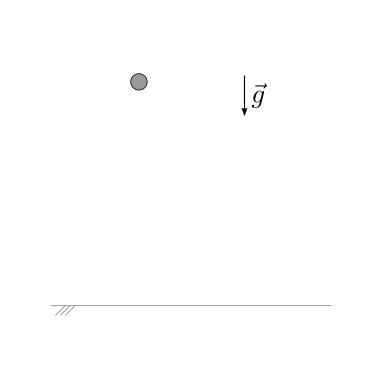
\includegraphics[width=.95\textwidth]{../../media/dynamics/free-fall.png}
\end{minipage}\\
\end{aligned}\end{align*}
\sphinxAtStartPar
\sphinxstylestrong{Soluzione.}
\begin{align*}\!\begin{aligned}
\begin{minipage}[t]{1.\textwidth}
  \vspace{0pt}
  \textbf{Problema 2.}
Viene chiesto di svolgere l'esercizio precedente, in un ambiente in cui non sia più trascurabile la resistenza aerodinamica del sistema.
In particolare viene chiesto di risolvere il problema nel caso in cui la resistenza aerodinamica sia:
1. proporzionale alla velocità relativa del corpo rispetto al fluido, di intensità $F = c v$, con $c = \dots$
2. proporzionale al quadrato della velocità relativa del corpo rispetto al fluido, di intensità $F = \frac{1}{2} \rho S c_F v^2$, con...\\
Qui si considera il fluido in quiete rispetto all'ambiente: la velocità del corpo relativa al fluido è quindi uguale alla velocità rispetto all'ambiente.\\
Viene chiesto poi di determinare la **velocità limite** raggiungibile da un corpo in caduta libera, potendo considerare l'accelerazione di gravità e la densità dell'aria costanti lungo la caduta.\\
\end{minipage}\\
\end{aligned}\end{align*}
\sphinxAtStartPar
\sphinxstylestrong{Soluzione.}
\begin{align*}\!\begin{aligned}
\begin{minipage}[t]{.55\textwidth}
  \vspace{0pt}
  \textbf{Problema 3.}
Un corpo di massa $m$ viene lanciato con velocità iniziale orizzontale con valore assoluto $|\vec{v}_0|$, da una quota $h$ sopra la superficie terrestre. Trascurando la resistenza aerodinamica, viene chiesto di determinare:
1. gittata
2. tempo di volo
3. velocità del corpo all'impatto con il suolo
4. impulso e forza media quando il corpo raggiunge terra, sapendo che il corpo si arresta in un tempo $\Delta t$ lungo una traiettoria rettilinea.\\
Come ulteriore esercizio, si ripetano i conti senza trascurare la resistenza aerodinamica.
\end{minipage}
\hspace{.05\textwidth}
\begin{minipage}[t]{.40\textwidth}
  \vspace{0pt}
  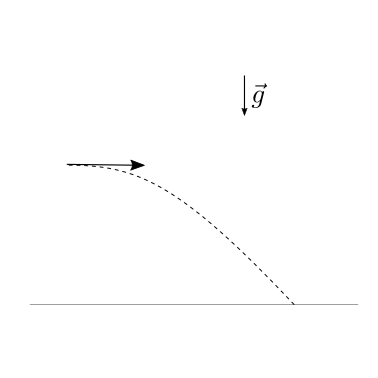
\includegraphics[width=.95\textwidth]{../../media/dynamics/parabolic-2.png}
\end{minipage}\\
\end{aligned}\end{align*}
\sphinxAtStartPar
\sphinxstylestrong{Soluzione.}
\begin{align*}\!\begin{aligned}
\begin{minipage}[t]{.55\textwidth}
  \vspace{0pt}
  \textbf{Problema 4.}
Viene chiesto di svolgere l'esercizio precedente, in un ambiente in cui non sia più trascurabile la resistenza aerodinamica del sistema.
In particolare viene chiesto di risolvere il problema nel caso in cui la resistenza aerodinamica sia:
1. proporzionale alla velocità relativa del corpo rispetto al fluido, di intensità $F = c v$, con $c = \dots$
2. proporzionale al quadrato della velocità relativa del corpo rispetto al fluido, di intensità $F = \frac{1}{2} \rho S c_F v^2$, con...\\
Qui si considera il fluido in quiete rispetto all'ambiente: la velocità del corpo relativa al fluido è quindi uguale alla velocità rispetto all'ambiente.\\
Viene chiesto poi di determinare la **velocità limite** raggiungibile da un corpo in caduta libera, potendo considerare l'accelerazione di gravità e la densità dell'aria costanti lungo la caduta.\\
\end{minipage}
\hspace{.05\textwidth}
\begin{minipage}[t]{.40\textwidth}
  \vspace{0pt}
  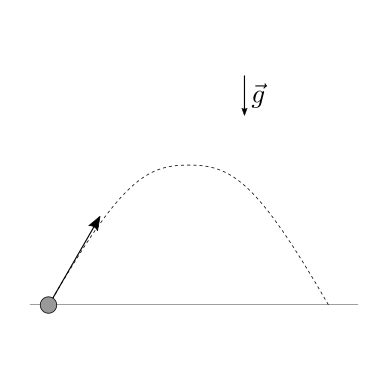
\includegraphics[width=.95\textwidth]{../../media/dynamics/parabolic-1.png}
\end{minipage}\\
\end{aligned}\end{align*}
\sphinxAtStartPar
\sphinxstylestrong{Soluzione.}
\begin{align*}\!\begin{aligned}
\begin{minipage}[t]{.55\textwidth}
  \vspace{0pt}
  \textbf{Problema 5.}
Conoscendo la posizione del punto di lancio $A$, e la posizione del bersaglio $B$ viene chiesto di determinare:
1. le condizioni sulla velocità di lancio per colpire il bersaglio. Una volta determinate, viene chiesto di determinare anche il tempo di volo.
2. tra tutte le velocità ammissibili per colpire il bersaglio, viene chiesto di determinare quella con valore assoluto minimo, sotto al quale non è possibile raggiungere l'obiettivo.\\
Come ulteriore esercizio, si ripetano i conti senza trascurare la resistenza aerodinamica.\\
\end{minipage}
\hspace{.05\textwidth}
\begin{minipage}[t]{.40\textwidth}
  \vspace{0pt}
  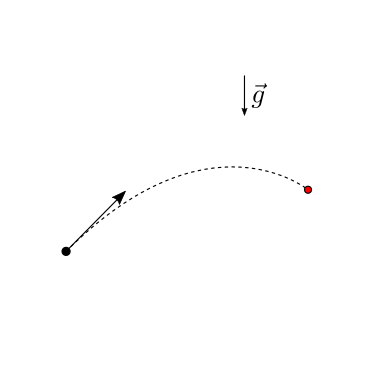
\includegraphics[width=.95\textwidth]{../../media/dynamics/parabolic-3.png}
\end{minipage}\\
\end{aligned}\end{align*}
\sphinxAtStartPar
\sphinxstylestrong{Soluzione.}
\begin{align*}\!\begin{aligned}
\begin{minipage}[t]{.55\textwidth}
  \vspace{0pt}
  \textbf{Problema 6.}
Conoscendo la posizione del punto di lancio $A$, e la posizione del bersaglio mobile $B: \vec{r}_B(t) = x_B \hat{x} + (y_{B,0} + v_{y,B} t) \hat{y}$ viene chiesto di determinare:
1. le condizioni sulla velocità di lancio per colpire il bersaglio. Una volta determinate, viene chiesto di determinare anche il tempo di volo.
2. tra tutte le velocità ammissibili per colpire il bersaglio, viene chiesto di determinare quella con valore assoluto minimo, sotto al quale non è possibile raggiungere l'obiettivo.\\
Come ulteriore esercizio, si ripetano i conti senza trascurare la resistenza aerodinamica.\\
\end{minipage}
\hspace{.05\textwidth}
\begin{minipage}[t]{.40\textwidth}
  \vspace{0pt}
  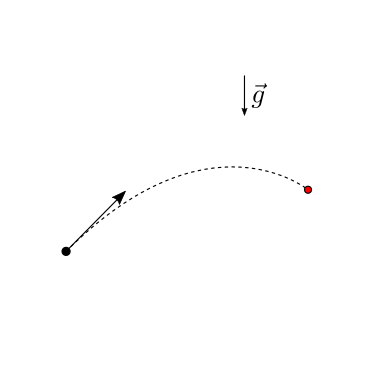
\includegraphics[width=.95\textwidth]{../../media/dynamics/parabolic-3.png}
\end{minipage}\\
\end{aligned}\end{align*}
\sphinxAtStartPar
\sphinxstylestrong{Soluzione.}
\begin{align*}\!\begin{aligned}
\begin{minipage}[t]{.55\textwidth}
  \vspace{0pt}
  \textbf{Problema 7.}
Un calciatore deve tirare una punizione in porta da una distanza $b$. La barriera viene posta a una distanza $a$ dal punto di tiro e i giocatori in barriera possono coprire fino a una quota $h$ saltando. Volendo centrare la porta a una quota $d$ (compresa tra $0$: la palla tocca terra sulla linea di porta senza rimbalzare prima; e $d_{max}$ la palla finisce all'incrocio), si chiede di determinare:
1. velocità iniziale imposta al pallone dal calcio
2. tempo di volo del pallone tra il calcio e la porta\\
in tutte le condizioni che permettono di prendere la porta senza colpire la barriera, e senza far rimbalzare il pallone prima della linea della porta. Per ogni valore $d$, si calcoli poi la condizione che corrisponde al tempo minore.\\
Si trascuri ogni effetto, dovuto alla rotazione del pallone.\\
Si svolga l'esercizio prima trascurando e poi considerando la resistenza aerodinamica.\\
**todo** Si può ampliare un po' l'esercizio considerando i tempi di reazione del portiere e la velocità nel comprire le distanze? O formulare qualche metodo per stimare la probabilità di realizzazione di calci di punizione...\\
\end{minipage}
\hspace{.05\textwidth}
\begin{minipage}[t]{.40\textwidth}
  \vspace{0pt}
  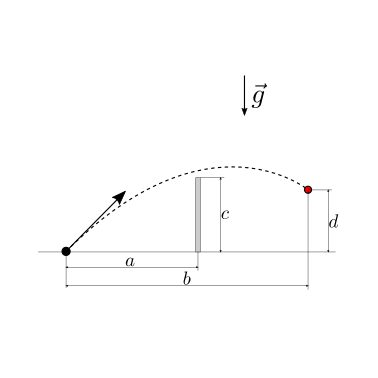
\includegraphics[width=.95\textwidth]{../../media/dynamics/parabolic-4.png}
\end{minipage}\\
\end{aligned}\end{align*}
\sphinxAtStartPar
\sphinxstylestrong{Soluzione.}
\begin{align*}\!\begin{aligned}
\begin{minipage}[t]{.55\textwidth}
  \vspace{0pt}
  \textbf{Problema 8.}
Un corpo puntiforme di massa $m$ è vincolato a una guida semi-circolare con un vincolo bilatero ideale (no attrito, solo reazione normale). Il corpo parte in condizioni di quiete da una posizione identificata da un raggio che forma un angolo $\theta_0$ con la verticale. Viene chiesto di:
1. rappresentare il diagramma delle forze agenti sul corpo;
2. scrivere l'espressione dell'energia meccanica del sistema, considerando il centro della semicriconferenza con punto di riferimento per definire l'energia potenziale gravitazionale nulla;
3. determinare la velocità massima del corpo nel suo moto
4. scrivere le equazioni del moto del sistema, usando **se possibile**: a) le equazioni cardinali della dinamica; b) la legge di conservazione dell'energia meccanica, c) altre leggi di conservazioni di quantità meccaniche costanti nella dinamica del sistema
5. determinare le reazioni vincolari della guida sul corpo puntiforme in funzione dell'angolo $\theta$ e daella sua derivata $\dot{\theta}$\\
\end{minipage}
\hspace{.05\textwidth}
\begin{minipage}[t]{.40\textwidth}
  \vspace{0pt}
  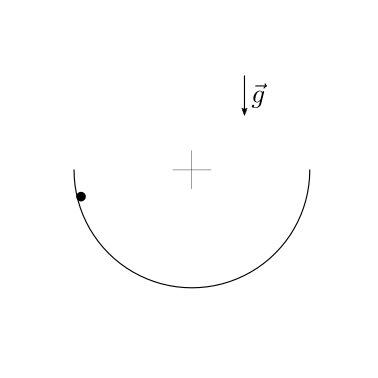
\includegraphics[width=.95\textwidth]{../../media/dynamics/arc-1.png}
\end{minipage}\\
\end{aligned}\end{align*}
\sphinxAtStartPar
\sphinxstylestrong{Soluzione.}
\begin{align*}\!\begin{aligned}
\begin{minipage}[t]{.55\textwidth}
  \vspace{0pt}
  \textbf{Problema 9.}
Un corpo puntiforme di massa $m$ è vincolato a una guida ad arco di cerchio con un vincolo bilatero ideale. Viene lasciato cadere da un angolo $\theta_0$ in condizioni di quiete. L'angolo "di uscita" della guida è $\theta_1$. Se ragginge l'angolo di uscita, il corpo è libero di compiere la traiettoria caratteristica del moto libero nella prossimità della superficie terrestre. Viene chiesto di determinare:
1. la velocità massima del corpo lungo la guida,
2. le condizioni per venire lanciato fuori dalla guida
3. la traiettoria del moto libero, determinando in particolare la gittata, il tempo di volo e la velocità di impatto.
4. sapendo che all'impatto il corpo viene rallentato dal terreno lungo una traiettoria rettilinea con una decelerazione costante $a$, si chiede di tereminare il tempo necessario all'arresto (a partire dall'impatto), l'impulso e la forza media.\\
Viene chiesto di discutere il problema considerando un attrito dinamico con coefficiente di attrito $\mu_d$ tra la guida e il corpo, rappresentando il diagramma delle forze agenti sul corpo e determinando le equazioni del moto lungo la guida.\\
\end{minipage}
\hspace{.05\textwidth}
\begin{minipage}[t]{.40\textwidth}
  \vspace{0pt}
  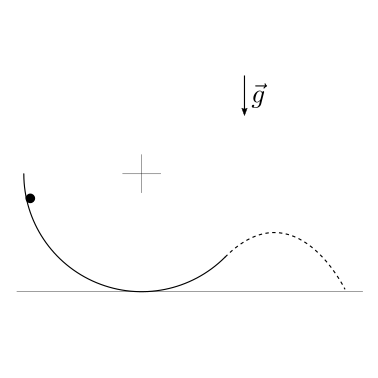
\includegraphics[width=.95\textwidth]{../../media/dynamics/arc-2.png}
\end{minipage}\\
\end{aligned}\end{align*}
\sphinxAtStartPar
\sphinxstylestrong{Soluzione.}
\begin{align*}\!\begin{aligned}
\begin{minipage}[t]{.55\textwidth}
  \vspace{0pt}
  \textbf{Problema 10.}
Una guida è formata da un primo tratto di raggio $R_1$, un secondo tratto di una circonferenza completa di raggio $R_2 < R_1$ e un terzo tratto rettilineo orizzontale. Trascurando l'attrito nei primi due tratti, viene chiesto di determinare:
1. le condizioni necessarie per poter compiere il loop del secondo tratto, nel caso di vincolo bilatero
2. le condizioni necessarie per poter compiere il loop del secondo tratto, nel caso di vincolo monolatero
3. la distanza percorsa sul terzo tratto orizzontale, sul quale non è possibile trascurare l'attrito con la guida, rappresentabile con la formula dell'attrito dinamico con coefficiente $\mu_d$.\\
Come esercizio aggiuntivo, viene chiesto di discutere il problema del moto del corpo con vincolo monolatero, nel caso in cui non sia in grado di compiere il loop.\\
\end{minipage}
\hspace{.05\textwidth}
\begin{minipage}[t]{.40\textwidth}
  \vspace{0pt}
  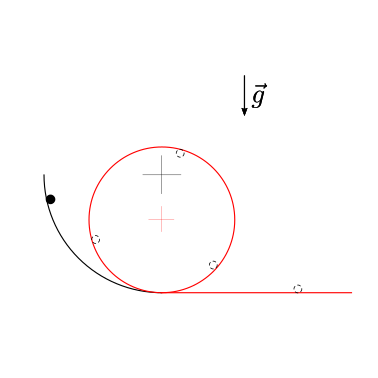
\includegraphics[width=.95\textwidth]{../../media/dynamics/arc-3.png}
\end{minipage}\\
\end{aligned}\end{align*}
\sphinxAtStartPar
\sphinxstylestrong{Soluzione.}
\begin{align*}\!\begin{aligned}
\begin{minipage}[t]{.55\textwidth}
  \vspace{0pt}
  \textbf{Problema 11.}
Conoscendo la configurazione iniziale della massa $m$, viene chiesto di descrivere la dinamica del sistema nel caso di attrito nullo e nel caso di attrito non trascurabile. Viene chiesto di:
1. determinare le equazioni del moto
2. risolvere le equazioni del moto
3. determinare le reazioni vincolari scambiate tra massa e parete obliqua
4. determinare la forza scambiata tra molla e parete, in funzione del tempo\\
\end{minipage}
\hspace{.05\textwidth}
\begin{minipage}[t]{.40\textwidth}
  \vspace{0pt}
  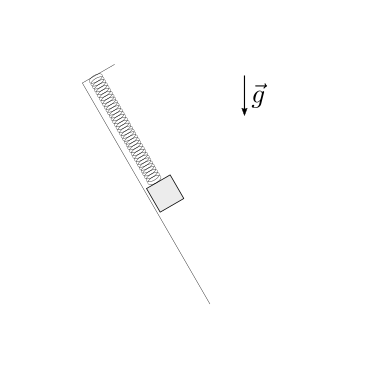
\includegraphics[width=.95\textwidth]{../../media/dynamics/oscillator-1.png}
\end{minipage}\\
\end{aligned}\end{align*}
\sphinxAtStartPar
\sphinxstylestrong{Soluzione.}
\begin{equation*}
\begin{split}
\begin{minipage}[t]{.55\textwidth}
  \vspace{0pt}
  \textbf{Problema 1.}
  Testo
\end{minipage}
\hspace{.05\textwidth}
\begin{minipage}[t]{.40\textwidth}
  \vspace{0pt}
  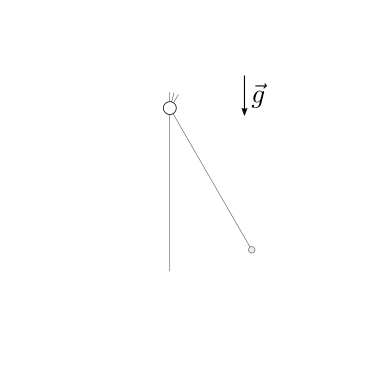
\includegraphics[width=.95\textwidth]{../../media/dynamics/oscillator-2-hinge.png}
\end{minipage}
\end{split}
\end{equation*}
\sphinxAtStartPar
\sphinxstylestrong{Soluzione.}
\begin{equation*}
\begin{split}
\begin{minipage}[t]{.55\textwidth}
  \vspace{0pt}
  \textbf{Problema 1.}
  Testo
\end{minipage}
\hspace{.05\textwidth}
\begin{minipage}[t]{.40\textwidth}
  \vspace{0pt}
  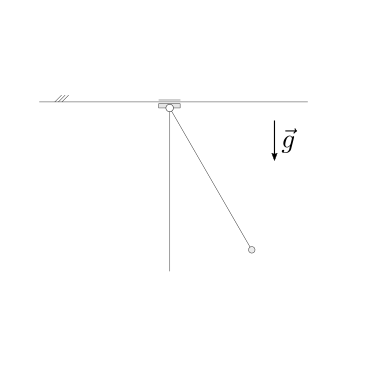
\includegraphics[width=.95\textwidth]{../../media/dynamics/oscillator-2-cart.png}
\end{minipage}
\end{split}
\end{equation*}
\sphinxAtStartPar
\sphinxstylestrong{Soluzione.}
\begin{equation*}
\begin{split}
\begin{minipage}[t]{.55\textwidth}
  \vspace{0pt}
  \textbf{Problema 1.}
  Testo
\end{minipage}
\hspace{.05\textwidth}
\begin{minipage}[t]{.40\textwidth}
  \vspace{0pt}
  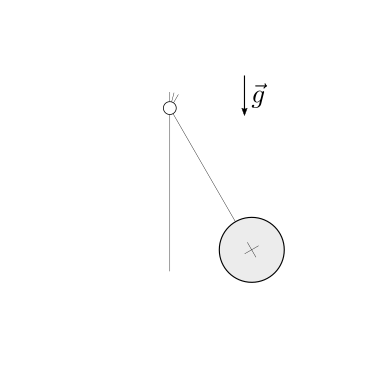
\includegraphics[width=.95\textwidth]{../../media/dynamics/oscillator-3-hinge.png}
\end{minipage}
\end{split}
\end{equation*}
\sphinxAtStartPar
\sphinxstylestrong{Soluzione.}
\begin{equation*}
\begin{split}
\begin{minipage}[t]{.55\textwidth}
  \vspace{0pt}
  \textbf{Problema 1.}
  Testo
\end{minipage}
\hspace{.05\textwidth}
\begin{minipage}[t]{.40\textwidth}
  \vspace{0pt}
  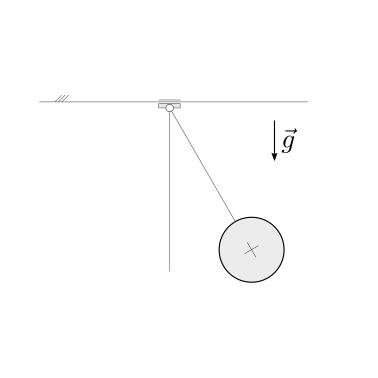
\includegraphics[width=.95\textwidth]{../../media/dynamics/oscillator-3-cart.png}
\end{minipage}
\end{split}
\end{equation*}
\sphinxAtStartPar
\sphinxstylestrong{Soluzione.}
\begin{equation*}
\begin{split}
\begin{minipage}[t]{.55\textwidth}
  \vspace{0pt}
  \textbf{Problema 1.}
  Testo
\end{minipage}
\hspace{.05\textwidth}
\begin{minipage}[t]{.40\textwidth}
  \vspace{0pt}
  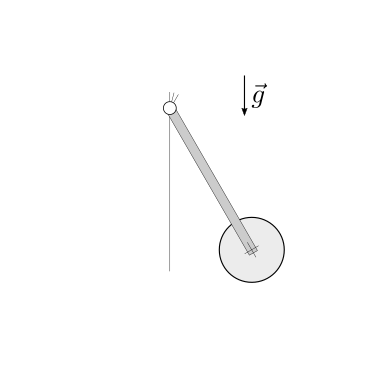
\includegraphics[width=.95\textwidth]{../../media/dynamics/oscillator-3-cart-hinge-rod.png}
\end{minipage}
\end{split}
\end{equation*}
\sphinxAtStartPar
\sphinxstylestrong{Soluzione.}
\begin{equation*}
\begin{split}
\begin{minipage}[t]{.55\textwidth}
  \vspace{0pt}
  \textbf{Problema 1.}
  Testo
\end{minipage}
\hspace{.05\textwidth}
\begin{minipage}[t]{.40\textwidth}
  \vspace{0pt}
  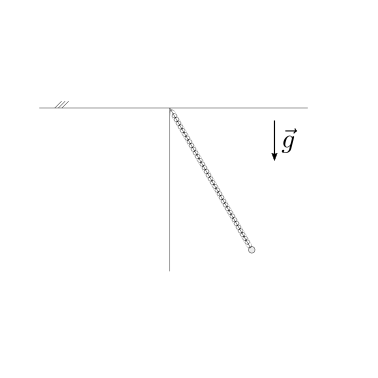
\includegraphics[width=.95\textwidth]{../../media/dynamics/oscillator-4-spring-hinge.png}
\end{minipage}
\end{split}
\end{equation*}
\sphinxAtStartPar
\sphinxstylestrong{Soluzione.}
\begin{equation*}
\begin{split}
\begin{minipage}[t]{.55\textwidth}
  \vspace{0pt}
  \textbf{Problema 1.}
  Testo
\end{minipage}
\hspace{.05\textwidth}
\begin{minipage}[t]{.40\textwidth}
  \vspace{0pt}
  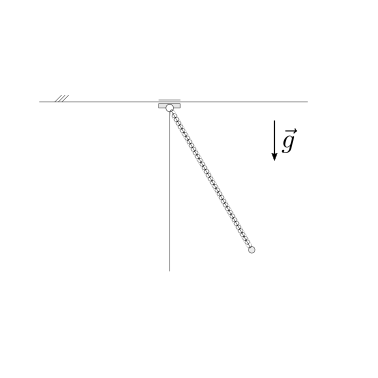
\includegraphics[width=.95\textwidth]{../../media/dynamics/oscillator-4-spring-cart.png}
\end{minipage}
\end{split}
\end{equation*}
\sphinxAtStartPar
\sphinxstylestrong{Soluzione.}
\begin{equation*}
\begin{split}
\begin{minipage}[t]{.55\textwidth}
  \vspace{0pt}
  \textbf{Problema 1.}
  Testo
\end{minipage}
\hspace{.05\textwidth}
\begin{minipage}[t]{.40\textwidth}
  \vspace{0pt}
  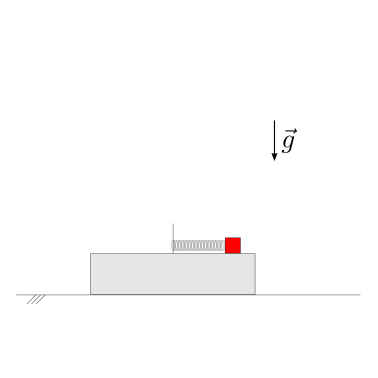
\includegraphics[width=.95\textwidth]{../../media/dynamics/oscillator-5-oscillator-point.png}
\end{minipage}
\end{split}
\end{equation*}
\sphinxAtStartPar
\sphinxstylestrong{Soluzione.}
\begin{equation*}
\begin{split}
\begin{minipage}[t]{.55\textwidth}
  \vspace{0pt}
  \textbf{Problema 1.}
  Testo
\end{minipage}
\hspace{.05\textwidth}
\begin{minipage}[t]{.40\textwidth}
  \vspace{0pt}
  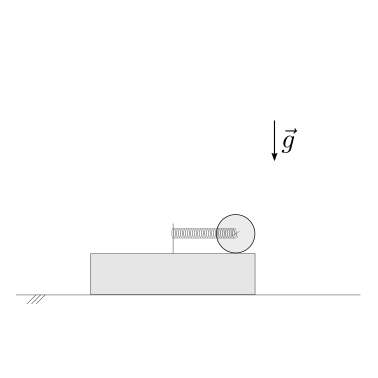
\includegraphics[width=.95\textwidth]{../../media/dynamics/oscillator-5-oscillator-disk.png}
\end{minipage}
\end{split}
\end{equation*}
\sphinxAtStartPar
\sphinxstylestrong{Soluzione.}
\begin{equation*}
\begin{split}
\begin{minipage}[t]{.55\textwidth}
  \vspace{0pt}
  \textbf{Problema 1.}
  Testo
\end{minipage}
\hspace{.05\textwidth}
\begin{minipage}[t]{.40\textwidth}
  \vspace{0pt}
  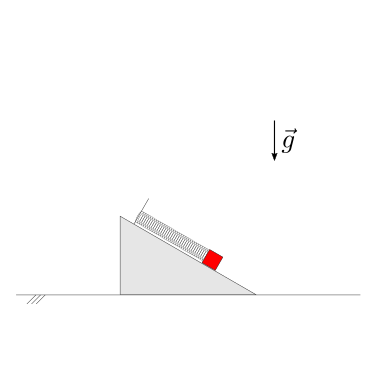
\includegraphics[width=.95\textwidth]{../../media/dynamics/oscillator-5-oscillator-prism-point.png}
\end{minipage}
\end{split}
\end{equation*}
\sphinxAtStartPar
\sphinxstylestrong{Soluzione.}
\begin{equation*}
\begin{split}
\begin{minipage}[t]{.55\textwidth}
  \vspace{0pt}
  \textbf{Problema 1.}
  Testo
\end{minipage}
\hspace{.05\textwidth}
\begin{minipage}[t]{.40\textwidth}
  \vspace{0pt}
  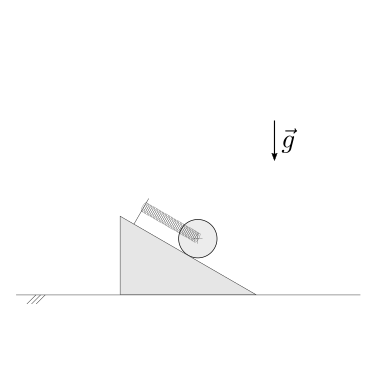
\includegraphics[width=.95\textwidth]{../../media/dynamics/oscillator-5-oscillator-prism-disk.png}
\end{minipage}
\end{split}
\end{equation*}
\sphinxAtStartPar
\sphinxstylestrong{Soluzione.}
\begin{equation*}
\begin{split}
\begin{minipage}[t]{.55\textwidth}
  \vspace{0pt}
  \textbf{Problema 1.}
  Testo
\end{minipage}
\hspace{.05\textwidth}
\begin{minipage}[t]{.40\textwidth}
  \vspace{0pt}
  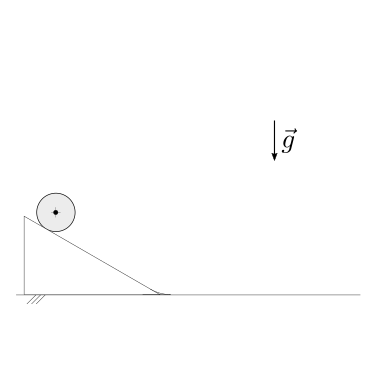
\includegraphics[width=.95\textwidth]{../../media/dynamics/ramp-6.png}
\end{minipage}
\end{split}
\end{equation*}
\sphinxAtStartPar
\sphinxstylestrong{Soluzione.}
\begin{equation*}
\begin{split}
\begin{minipage}[t]{.55\textwidth}
  \vspace{0pt}
  \textbf{Problema 1.}
  Testo
\end{minipage}
\hspace{.05\textwidth}
\begin{minipage}[t]{.40\textwidth}
  \vspace{0pt}
  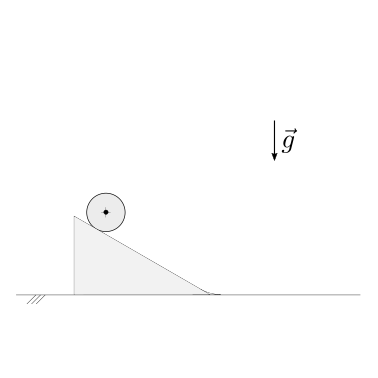
\includegraphics[width=.95\textwidth]{../../media/dynamics/ramp-6-moving.png}
\end{minipage}
\end{split}
\end{equation*}
\sphinxAtStartPar
\sphinxstylestrong{Soluzione.}
\begin{equation*}
\begin{split}
\begin{minipage}[t]{.55\textwidth}
  \vspace{0pt}
  \textbf{Problema 1.}
  Testo
\end{minipage}
\hspace{.05\textwidth}
\begin{minipage}[t]{.40\textwidth}
  \vspace{0pt}
  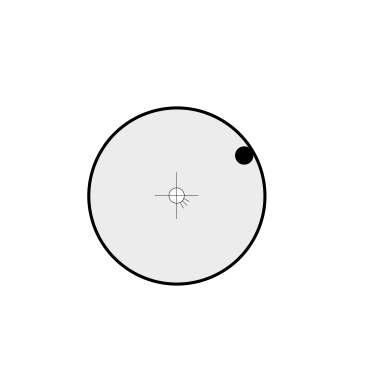
\includegraphics[width=.95\textwidth]{../../media/dynamics/eccentric-6-0.png}
\end{minipage}
\end{split}
\end{equation*}
\sphinxAtStartPar
\sphinxstylestrong{Soluzione.}
\begin{equation*}
\begin{split}
\begin{minipage}[t]{.55\textwidth}
  \vspace{0pt}
  \textbf{Problema 1.}
  Testo
\end{minipage}
\hspace{.05\textwidth}
\begin{minipage}[t]{.40\textwidth}
  \vspace{0pt}
  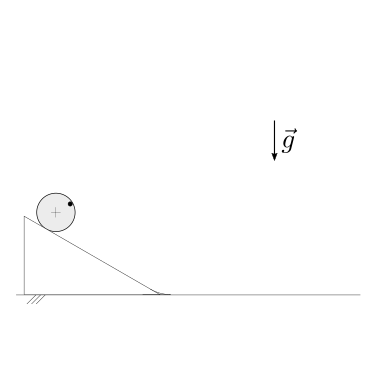
\includegraphics[width=.95\textwidth]{../../media/dynamics/eccentric-6-1.png}
\end{minipage}
\end{split}
\end{equation*}
\sphinxAtStartPar
\sphinxstylestrong{Soluzione.}
\begin{equation*}
\begin{split}
\begin{minipage}[t]{.55\textwidth}
  \vspace{0pt}
  \textbf{Problema 1.}
  Testo
\end{minipage}
\hspace{.05\textwidth}
\begin{minipage}[t]{.40\textwidth}
  \vspace{0pt}
  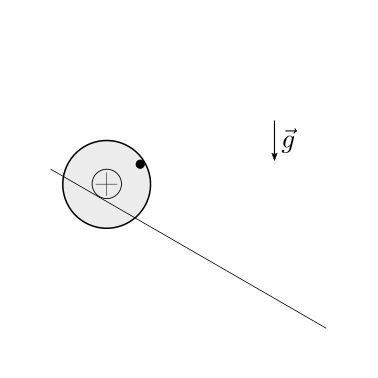
\includegraphics[width=.95\textwidth]{../../media/dynamics/eccentric-6-2.png}
\end{minipage}
\end{split}
\end{equation*}
\sphinxAtStartPar
\sphinxstylestrong{Soluzione.}
\begin{equation*}
\begin{split}
\begin{minipage}[t]{.55\textwidth}
  \vspace{0pt}
  \textbf{Problema 1.}
  Testo
\end{minipage}
\hspace{.05\textwidth}
\begin{minipage}[t]{.40\textwidth}
  \vspace{0pt}
  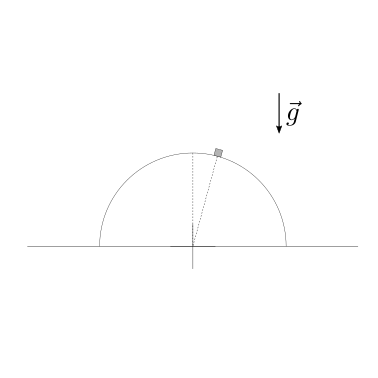
\includegraphics[width=.95\textwidth]{../../media/dynamics/detach-7-point.png}
\end{minipage}
\end{split}
\end{equation*}
\sphinxAtStartPar
\sphinxstylestrong{Soluzione.}
\begin{equation*}
\begin{split}
\begin{minipage}[t]{.55\textwidth}
  \vspace{0pt}
  \textbf{Problema 1.}
  Testo
\end{minipage}
\hspace{.05\textwidth}
\begin{minipage}[t]{.40\textwidth}
  \vspace{0pt}
  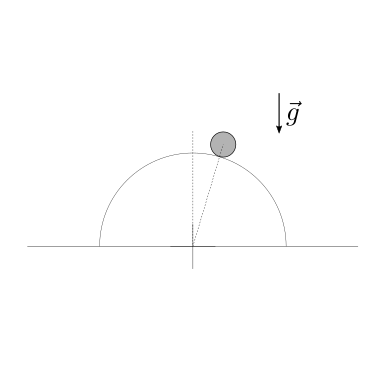
\includegraphics[width=.95\textwidth]{../../media/dynamics/detach-7-disk.png}
\end{minipage}
\end{split}
\end{equation*}
\sphinxAtStartPar
\sphinxstylestrong{Soluzione.}
\begin{equation*}
\begin{split}
\begin{minipage}[t]{.55\textwidth}
  \vspace{0pt}
  \textbf{Problema 1.}
  Testo
\end{minipage}
\hspace{.05\textwidth}
\begin{minipage}[t]{.40\textwidth}
  \vspace{0pt}
  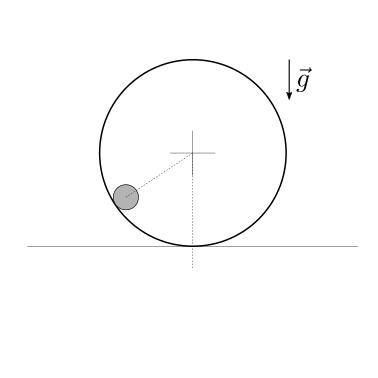
\includegraphics[width=.95\textwidth]{../../media/dynamics/oscillator-8-ring-disk.png}
\end{minipage}
\end{split}
\end{equation*}
\sphinxAtStartPar
\sphinxstylestrong{Soluzione.}
\begin{equation*}
\begin{split}
\begin{minipage}[t]{.55\textwidth}
  \vspace{0pt}
  \textbf{Problema 1.}
  Testo
\end{minipage}
\hspace{.05\textwidth}
\begin{minipage}[t]{.40\textwidth}
  \vspace{0pt}
  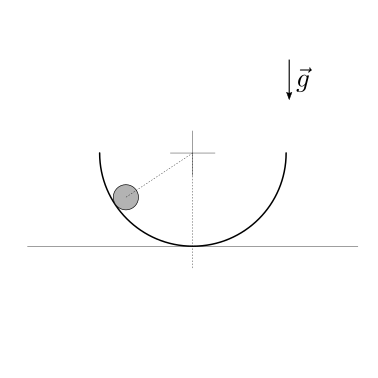
\includegraphics[width=.95\textwidth]{../../media/dynamics/oscillator-8-ring-half-disk.png}
\end{minipage}
\end{split}
\end{equation*}
\sphinxAtStartPar
\sphinxstylestrong{Soluzione.}





\sphinxstepscope


\section{Note e dimostrazioni}
\label{\detokenize{ch/mechanics/dynamics-notes:note-e-dimostrazioni}}\label{\detokenize{ch/mechanics/dynamics-notes:physics-hs-mechanics-dynamics-notes}}\label{\detokenize{ch/mechanics/dynamics-notes::doc}}

\subsection{Equazioni cardinali della dinamica per un punto}
\label{\detokenize{ch/mechanics/dynamics-notes:equazioni-cardinali-della-dinamica-per-un-punto}}\label{\detokenize{ch/mechanics/dynamics-notes:physics-hs-mechanics-dynamics-eom-point}}
\sphinxAtStartPar
Le equazioni cardinali della dinamica in forma differenziale,
\begin{equation*}
\begin{split}\begin{aligned}
 \dot{\vec{Q}} & = \vec{R}^{ext} & \text{(bilancio quantità di moto)} \\
 \dot{\vec{L}}_H + \dot{\vec{x}}_H \times \vec{Q} & = \vec{M}_H^{ext} & \text{(bilancio momento della quantità di moto)} \\
 \dot{K} & = P^{tot} & \text{(bilancio energia cinetica)} \ .
\end{aligned}\end{split}
\end{equation*}
\sphinxAtStartPar
vengono ricavate per un sistema puntiforme calcolando la derivata nel tempo delle grandezze dinamiche di un punto,
\begin{equation*}
\begin{split}\begin{aligned}
  \vec{Q}_P & := m_P \vec{v}_P  & \text{(quantità di moto)} \\
  \vec{L}_{P,H} & := (\vec{r}_P - \vec{r}_H) \times \vec{Q} = m_P (\vec{r}_P - \vec{r}_H) \times \vec{v}_P & \text{(momento della quantità di moto)} \\
  K & := \frac{1}{2} m_P \vec{v}_P \cdot \vec{v}_P = \frac{1}{2} m_P |\vec{v}_P|^2 & \text{(energia cinetica)}
\end{aligned}\end{split}
\end{equation*}
\sphinxAtStartPar
utilizzando i princìpi della dinamica.
\subsubsection*{Bilancio della quantità di moto}

\sphinxAtStartPar
Il bilancio della quantità di moto di un punto materiale \(P\), \(\vec{Q}_P = m \vec{v}_P\) segue direttamente dal secondo principio della dinamica di Newton,
\begin{equation*}
\begin{split}\dot{\vec{Q}}_P = \vec{R}^{ext}_P\end{split}
\end{equation*}\subsubsection*{Bilancio del momento della quantità di moto}

\sphinxAtStartPar
La derivata nel tempo del momento della quantità di moto viene calcolata usando la regola del prodotto,
\begin{equation*}
\begin{split}\begin{aligned}
\dot{\vec{L}}_{P,H} & = \dfrac{d}{dt} \left[ m_P (\vec{r}_P - \vec{r}_H) \times \vec{v}_P \right] = \\
& = m \left[ ( \dot{\vec{r}}_P - \dot{\vec{r}}_H ) \times \vec{v}_P + m_P (\vec{r}_P - \vec{r}_H) \times \dot{\vec{v}}_P \right] = \\
& = - m_P \dot{\vec{r}}_H \times \vec{v}_P + m_P (\vec{r}_P - \vec{r}_H) \times \dot{\vec{v}}_P = \\
& = - \dot{\vec{r}}_H \times \vec{Q} + \vec{M}_H^{ext} \ .
\end{aligned}\end{split}
\end{equation*}\subsubsection*{Bilancio dell’energia cinetica.}
\begin{equation*}
\begin{split}\begin{aligned}
\dot{K}_{P} & = \dfrac{d}{dt} \left( \frac{1}{2} m_P \vec{v}_P \cdot \vec{v}_P \right) = \\
            & = m_P \dot{\vec{v}}_P \cdot \vec{v}_P = \\
            & = \vec{R}^{ext} \cdot \vec{v}_P = \\
            & = \vec{R}^{tot} \cdot \vec{v}_P = P^{tot} \ .
\end{aligned}\end{split}
\end{equation*}

\subsection{Equazioni cardinali della dinamica per sistemi di punti}
\label{\detokenize{ch/mechanics/dynamics-notes:equazioni-cardinali-della-dinamica-per-sistemi-di-punti}}\label{\detokenize{ch/mechanics/dynamics-notes:physics-hs-mechanics-dynamics-eom-points}}
\sphinxAtStartPar
Partendo dalle equazioni dinamiche per un punto, si ricavano le equazioni dinamiche per un sistema di punti,
\begin{equation*}
\begin{split}\begin{aligned}
 \dot{\vec{Q}} & = \vec{R}^{ext} & \text{(bilancio quantità di moto)} \\
 \dot{\vec{L}}_H + \dot{\vec{x}}_H \times \vec{Q} & = \vec{M}_H^{ext} & \text{(bilancio momento della quantità di moto)} \\
 \dot{K} & = P^{tot} & \text{(bilancio energia cinetica)} \ .
\end{aligned}\end{split}
\end{equation*}
\sphinxAtStartPar
sfruttando il terzo principio della dinamica di azione/reazione. Lo sviluppo delle equazioni permette di comprendere l’origine della natura additiva delle grandezze dinamiche di sistemi composti da più componenti,
\begin{equation*}
\begin{split}\begin{aligned}
\vec{Q}     & = \sum_i \vec{Q}_i     & \text{(quantità di moto)}\\
\vec{L}_{H} & = \sum_i \vec{L}_{H,i} & \text{(momento della quantità di moto)}\\
 K          & = \sum_i K_i           & \text{(energia cinetica)} \ .
\end{aligned}\end{split}
\end{equation*}
\sphinxAtStartPar
(quantità di moto, momento della quantità di moto, energia cinetica),
\subsubsection*{Bilancio della quantità di moto.}

\sphinxAtStartPar
E” possibile scrivere il bilancio della quantità di moto per ogni punto \(i\) del sistema, scrivendo la risultante delle forze esterne agente sul punto come la somma delle forze esterne all’intero sistema agenti sul punto e le forze interne scambiate con gli altri punti del sistema,
\begin{equation*}
\begin{split}\vec{R}_i^{ext,i} = \vec{F}_i^{ext} + \sum_{j \ne i} \vec{F}_{ij} \ .\end{split}
\end{equation*}
\sphinxAtStartPar
L’equazione di bilancio per la \(i\)\sphinxhyphen{}esima massa diventa quindi
\begin{equation*}
\begin{split}\dot{\vec{Q}}_i = \vec{R}_i^{ext,i} = \vec{F}_i^{ext} + \sum_{j \ne i} \vec{F}_{ij} \ .\end{split}
\end{equation*}
\sphinxAtStartPar
Sommando le equazioni di bilancio di tutte le masse, si ottiene
\begin{equation*}
\begin{split}\begin{aligned}
\sum_{i} \dot{\vec{Q}}_i & = \sum_i \vec{F}_{i}^{ext} + \sum_i \sum_{j \ne i} \vec{F}_{ij} = \\
                            & = \sum_i \vec{F}_{i}^{ext} + \sum_{\{i,j\}} \underbrace{\left( \vec{F}_{ij} + \vec{F}_{ji} \right)}_{=\vec{0}} 
\end{aligned}\end{split}
\end{equation*}
\sphinxAtStartPar
e definendo la quantità di moto di un sistema come la somma delle quantità di moto delle sue parti e la risultante delle forze esterne come somma delle forze esterne agenti sulle parti del sistema,
\begin{equation*}
\begin{split}\vec{Q} := \sum_i \vec{Q}\end{split}
\end{equation*}\begin{equation*}
\begin{split}\vec{R}^{ext} := \sum_i \vec{F}_i^{ext}\end{split}
\end{equation*}
\sphinxAtStartPar
si ritrova la forma generale del bilancio della quantità di moto,
\begin{equation*}
\begin{split}\dot{\vec{Q}} = \vec{R}^{ext} \ .\end{split}
\end{equation*}\subsubsection*{Bilancio del momento della quantità di moto}

\sphinxAtStartPar
E” possibile scrivere il bilancio del momento della quantità di moto per ogni punto \(i\) del sistema, scrivendo la risultante dei momenti esterni agente sul punto come la somma dei momenti esterni all’intero sistema agenti sul punto e i momenti interni scambiati con gli altri punti del sistema,
\begin{equation*}
\begin{split}\vec{M}_{H,i}^{ext,i} = \vec{M}_{H,i}^{ext} + \sum_{j \ne i} \vec{M}_{H,ij} \ .\end{split}
\end{equation*}
\sphinxAtStartPar
Nel caso le parti del sistema interagiscano tramite forze, il momento rispetto al polo \(H\) generato dalla massa \(j\) sulla massa \(i\) vale
\begin{equation*}
\begin{split}\vec{M}_{H,ij} = (\vec{r}_i - \vec{r}_H) \times \vec{F}_{ij} \ .\end{split}
\end{equation*}
\sphinxAtStartPar
L’equazione di bilancio per la \(i\)\sphinxhyphen{}esima massa diventa quindi
\begin{equation*}
\begin{split}\dot{\vec{L}}_{H,i} + \dot{\vec{r}}_H \times \vec{Q}_i = \vec{M}_{H,i}^{ext,i} = \vec{M}_{H,i}^{ext} + \sum_{j \ne i} \vec{M}_{H,ij} \ .\end{split}
\end{equation*}
\sphinxAtStartPar
Sommando le equazioni di bilancio di tutte le masse, si ottiene
\begin{equation*}
\begin{split}\begin{aligned}
\sum_{i} \left( \dot{\vec{L}}_i + \dot{\vec{r}}_H \times \vec{Q}_i \right) & = \sum_i \vec{M}_{H,i}^{ext} + \sum_i \sum_{j \ne i} \vec{M}_{H,ij} = \\
                            & = \sum_i \vec{M}_{H,i}^{ext} + \sum_{\{i,j\}} \underbrace{\left( \vec{M}_{H,ij} + \vec{M}_{H,ji} \right)}_{=\vec{0}} 
\end{aligned}\end{split}
\end{equation*}
\sphinxAtStartPar
e riconoscendo la quantità di moto del sistema e definendo il momento della quantità di moto di un sistema come la somma del momento della quantità di moto delle sue parti e la risultante dei momenti esterni come somma dei momenti esterni agenti sulle parti del sistema,
\begin{equation*}
\begin{split}\vec{L}_H := \sum_i \vec{L}_{H,i}\end{split}
\end{equation*}\begin{equation*}
\begin{split}\vec{M}_H^e := \sum_i \vec{M}_{H,i}^{ext}\end{split}
\end{equation*}
\sphinxAtStartPar
si ritrova la forma generale del bilancio del momento della quantità di moto,
\begin{equation*}
\begin{split}\dot{\vec{L}}_{H} + \dot{\vec{r}}_H \times \vec{Q} = \vec{M}_H^{ext} \ .\end{split}
\end{equation*}\subsubsection*{Bilancio dell’energia cinetica.}

\sphinxAtStartPar
E” possibile ricavare il bilancio dell’energia cinetica del sistema, moltiplicando scalarmente il bilancio della quantità di moto di ogni punto,
\begin{equation*}
\begin{split}\vec{v}_i \cdot m_i \dot{\vec{v}}_i = \vec{v}_i \cdot \left( \vec{F}_i^{e} + \sum_{j \ne i} \vec{F}_{ij} \right) \ ,\end{split}
\end{equation*}
\sphinxAtStartPar
riconoscendo nel primo termine la derivata nel tempo dell’energia cinetica dell”\(i\)\sphinxhyphen{}esimo punto,
\begin{equation*}
\begin{split}\dot{K}_i = \dfrac{d}{dt} \left( \frac{1}{2} m_i \vec{v}_i \cdot \vec{v}_i \right) = m_i \vec{v}_i \cdot \dot{\vec{v}}_i \ ,\end{split}
\end{equation*}
\sphinxAtStartPar
e sommando queste equazioni di bilancio per ottenere
\begin{equation*}
\begin{split}\begin{aligned}
  \sum_i \dot{K}_i = \sum_i \vec{v}_i \cdot  \vec{F}_i^{e} + \sum_i \vec{v}_i \cdot \sum_{j \ne i} \vec{F}_{ij} \ . 
\end{aligned}\end{split}
\end{equation*}
\sphinxAtStartPar
Definendo l’energia cinetica di un sistema come la somma dell’energia cinetica delle sue parti, e definendo la potenza delle forze esterne/interne agenti sul sistema come la somma della potenza di tutte le forze esterne/interni al sistema,
\begin{equation*}
\begin{split}K :=  \sum_i K_i\end{split}
\end{equation*}\begin{equation*}
\begin{split}P^e := \sum_i P^{ext}_i = \sum_i \vec{v}_i \cdot  \vec{F}_i^{ext} \end{split}
\end{equation*}\begin{equation*}
\begin{split}P^i := \sum_i P^{int}_i = \sum_i \vec{v}_i \cdot \sum_{j \ne i} \vec{F}_{ij}\end{split}
\end{equation*}
\sphinxAtStartPar
si ritrova la forma generale del bilancio dell’energia cinetica,
\begin{equation*}
\begin{split}\dot{K} = P^{ext} + P^{int} = P^{tot} \ .\end{split}
\end{equation*}

\section{Equazioni cardinali della dinamica per un corpo rigido in moto piano}
\label{\detokenize{ch/mechanics/dynamics-notes:equazioni-cardinali-della-dinamica-per-un-corpo-rigido-in-moto-piano}}\label{\detokenize{ch/mechanics/dynamics-notes:physics-hs-mechanics-dynamics-eom-rigid-2d}}
\sphinxAtStartPar
\sphinxstylestrong{todo}

\sphinxstepscope


\part{Cenni di meccanica del continuo}

\sphinxstepscope


\chapter{Cenni di meccanica del continuo}
\label{\detokenize{ch/continuum/intro:cenni-di-meccanica-del-continuo}}\label{\detokenize{ch/continuum/intro:physics-hs-continuum}}\label{\detokenize{ch/continuum/intro::doc}}

\section{Fluidi}
\label{\detokenize{ch/continuum/intro:fluidi}}\label{\detokenize{ch/continuum/intro:continuum-fluids}}

\subsection{Statica dei fluidi}
\label{\detokenize{ch/continuum/intro:statica-dei-fluidi}}\label{\detokenize{ch/continuum/intro:fluids-statics}}

\subsection{Dinamica dei fluidi}
\label{\detokenize{ch/continuum/intro:dinamica-dei-fluidi}}\label{\detokenize{ch/continuum/intro:fluids-dynamics}}

\subsection{Bilancio di quantità di moto, energia e teorema di Bernoulli}
\label{\detokenize{ch/continuum/intro:bilancio-di-quantita-di-moto-energia-e-teorema-di-bernoulli}}\label{\detokenize{ch/continuum/intro:fluids-dynamics-bernoulli}}

\subsection{Legge di Stokes}
\label{\detokenize{ch/continuum/intro:legge-di-stokes}}\label{\detokenize{ch/continuum/intro:fluids-dynamics-stokes}}
\sphinxAtStartPar
L’interazione tra un fluido e un corpo di piccole dimensioni in moto relativo rispetto al fluido con \sphinxstyleemphasis{velocità relativa} \(\vec{v}_{rel}\) rispetto alla velocità del fluido locale si manifesta come una forza di resistenza aerodinamica. Per un corpo sferico di raggio \(R\), la formula di Stokes fornisce un’espressione \sphinxstyleemphasis{esatta} (\sphinxstyleemphasis{esatta all’interno del modello usato}) di questa forza
\begin{equation*}
\begin{split}\vec{F} = - 6 \pi \mu R \vec{v}_{rel} \ .\end{split}
\end{equation*}
\sphinxAtStartPar
La formula di Stokes fornisce un’espressione della resistenza aerodinamcia lineare rispetto alla velocità relativa.

\sphinxAtStartPar
\sphinxstylestrong{todo} \sphinxstyleemphasis{Commentare effetto di \textbackslash{}text\{Re\}. Cogliere l’occasione per un po” di analisi dimensionale per ottenere la formula \(\vec{F} = \frac{1}{2} \rho |\vec{v}|^2 \vec{c}_F(\text{Re}, \text{M})\)…}


\section{Solidi}
\label{\detokenize{ch/continuum/intro:solidi}}\label{\detokenize{ch/continuum/intro:continuum-solids}}\begin{itemize}
\item {} 
\sphinxAtStartPar
Solidi elastici

\end{itemize}


\section{todo}
\label{\detokenize{ch/continuum/intro:todo}}\begin{itemize}
\item {} 
\sphinxAtStartPar
Cenni di propagazione perturbazioni come onde, es:
\begin{itemize}
\item {} 
\sphinxAtStartPar
fluidi:
\begin{itemize}
\item {} 
\sphinxAtStartPar
pressione e acustica, piccole perturbazioni e urti

\item {} 
\sphinxAtStartPar
onde con superficie libera (mare, rubinetto,…)

\end{itemize}

\item {} 
\sphinxAtStartPar
perturbazioni nei solidi:
\begin{itemize}
\item {} 
\sphinxAtStartPar
corda di una chitarra; altri esempi con elementi 1d

\item {} 
\sphinxAtStartPar
esempi con membrane (es, nostro orecchio)

\item {} 
\sphinxAtStartPar
esempi di propagazione in mezzi (più o meno) continui

\item {} 
\sphinxAtStartPar
onde sismiche

\end{itemize}

\end{itemize}

\end{itemize}

\sphinxstepscope


\part{Termodinamica}

\sphinxstepscope


\chapter{Introduzione alla termodinamica}
\label{\detokenize{ch/thermodynamics/foundation:introduzione-alla-termodinamica}}\label{\detokenize{ch/thermodynamics/foundation:physics-hs-thermodynamics-intro}}\label{\detokenize{ch/thermodynamics/foundation::doc}}
\sphinxAtStartPar
La termodinamica è la branca della fisica che si occupa dell’energia, della trasformazione tra le varie forme di energia e dei meccanismi che permettono di variare l’energia di un sistema.

\sphinxAtStartPar
La \sphinxstylestrong{termodinamica classica} fornisce una \sphinxstylestrong{descrizione macroscopica}, media, di sistemi complessi costituiti da un gran numero di componenti elementari in \sphinxstylestrong{equilibrio} statistico a livello microscopico. Sebbene il \sphinxstylestrong{modello atomistico} (\sphinxstylestrong{todo} \sphinxstyleemphasis{link?}) della materia rappresenti uno dei più grandi successi della storia della scienza secondo Feynman, per la sua utilità nella comprensione intima di molti fenomeni fisici, in molte occasioni questo modello contiene troppe informazioni \sphinxhyphen{} molte più informazioni di quelle necessarie in molti ambiti \sphinxhyphen{} e risulta non pratico: così, ad esempio possiamo descrivere le condizioni in una stanza in termini di temperatura \sphinxhyphen{} una \sphinxstylestrong{(!)} variabile macroscopica, due se aggiungiamo l’informazione di pressione \sphinxhyphen{} e non descrivendo la dinamica delle \(N\) molecole dei gas che formano l’aria che respiriamo \sphinxhyphen{} per le quali servirebbero \(\sim 10^{26}\) grandezze fisiche per una stanza di \(10 \, m^3\), o comunque \(\sim 10^{19}\) per ogni \(\text{cm}^3\). La \sphinxstylestrong{meccanica statistica} (\sphinxstylestrong{todo} \sphinxstyleemphasis{link?}) fornisce il ponte tra le due descrizioni, ritrovando la termodinamica classica come media della descrizione microscopica.
\subsubsection*{Feynman e la teoria atomica}

\sphinxAtStartPar
La prima lezione%
\begin{footnote}[1]\sphinxAtStartFootnote
\sphinxurl{https://www.feynmanlectures.caltech.edu/I\_01.html}
%
\end{footnote} di fisica delle lezioni di fisica di Feynman, \sphinxstyleemphasis{The Feynman Lectures on Physics, Volume I} %
\begin{footnote}[2]\sphinxAtStartFootnote
\sphinxurl{https://www.feynmanlectures.caltech.edu/I\_toc.html}
%
\end{footnote} riguarda la teoria atomica. Feynman riconosce il ruolo fondamentale della teoria atomica nella scienza,
\begin{quote}

\sphinxAtStartPar
If, in some cataclysm, all of scientific knowledge were to be destroyed, and only one sentence passed on to the next generations of creatures, what statement would contain the most information in the fewest words? I believe it is the atomic hypothesis (or the atomic fact, or whatever you wish to call it) that all things are made of atoms—little particles that move around in perpetual motion, attracting each other when they are a little distance apart, but repelling upon being squeezed into one another. In that one sentence, you will see, there is an enormous amount of information about the world, if just a little imagination and thinking are applied.
\end{quote}






\bigskip\hrule\bigskip


\sphinxstepscope


\section{Breve storia della termodinamica}
\label{\detokenize{ch/thermodynamics/foundation-history:breve-storia-della-termodinamica}}\label{\detokenize{ch/thermodynamics/foundation-history:physics-hs-thermodynamics-foundation-history}}\label{\detokenize{ch/thermodynamics/foundation-history::doc}}
\sphinxAtStartPar
La termodinamica ha avuto uno sviluppo non lineare, dovuto al contributo di molti studiosi in ambiti diversi, nel corso di più di un paio di secoli.

\sphinxAtStartPar
\sphinxstylestrong{Brevissima storia della termodinamica.}
Durante la rivoluzione scientifica del XVI\sphinxhyphen{}XVII secolo, la progettazione di strumenti di misura basati sulla dilatazione delle sostanze e la diffusione del metodo sperimentale in ambito scientifico hanno permesso di introdurre le grandezze fisiche di pressione e temperatura; la misura della massa delle sostanze negli esperimenti di chimica ha permesso a Lavoisier di formulare il principio di conservazione della massa, e formulare l’ipotesi atomistica della struttura della materia, usata da Bernoulli per formulare la teoria cinetica dei gas; le attività di Black sul cambiamento di fase delle sostanze permettono di chiarire la differenza tra temperatura e calore; la macchina a vapore strutta il calore come fonte di lavoro meccanico, svolgendo un ruolo fondamentale nella rivoluzione industriale del XVIII secolo; l’indagine sulle reazioni chimiche e sui gas fornisce nuovi dettagli sulla natura della materia e ulteriori argomenti a supporto della “ipotesi atomistica; l’analisi teoria di Carnot sulle macchine termiche e sul loro rendimento conduce ai risultati di equivalenza di Joule sull’equivalenza lavoro\sphinxhyphen{}calore nel bilancio di energia di un sistema, che porta a formulare il primo principio della termodinamica. L’equivalenza tra calore e lavoro non è però perfetta, come evidenziato dal secondo principio della termodinamica enunciato da Clausis, che riassume le tendenze naturali nella trasmissione del calore e della dissipazione del lavoro meccanico in calore introducendo il concetto di entropia. Verso la fine del XIX secolo, Gibbs elabora una formalizzazione matematica rigorosa della termodinamica classica, usata in gran parte ancora oggi: grazie i concetti di energia interna di un sistema, potenziali termodinamici e stato termodinamico di un sistema, la teoria di Gibbs fornisce un modello macroscopico rigoroso per l’analisi di sistemi termodinamici che coinvolgono trasformazioni e trasferimenti di energia, tramite lavoro, calore o reazioni chimiche.
Gibbs, Maxwell, Boltzmann e la nascita della meccanica statistica…

\sphinxAtStartPar
\sphinxstylestrong{Dalle esperienze alla comprensione.}
Dalla sensazione di caldo\sphinxhyphen{}freddo,…, a un modello…



\sphinxAtStartPar
\sphinxstylestrong{Indagine scientifica: natura materia.} Rivoluzione scientifica del XVI\sphinxhyphen{}XVII secolo. Costruzione di strumenti
\begin{itemize}
\item {} 
\sphinxAtStartPar
Torricelli, disceplo di Galileo:
\begin{itemize}
\item {} 
\sphinxAtStartPar
il barometro;

\item {} 
\sphinxAtStartPar
la misura del peso dell’aria: \sphinxstylestrong{pressione} atmosferica;

\item {} 
\sphinxAtStartPar
«vuoto» al di sopra della colonnina di Hg: argomento che rilancia la tesi atomistica

\end{itemize}

\item {} 
\sphinxAtStartPar
Boyle, «primo chimico»; tra i fondatori della Royal Society; preciso sperimentatore (descrizione dettagliata per permettere replica), grazie agli strumenti progettati e realizzati da Robert Hooke:
\begin{itemize}
\item {} 
\sphinxAtStartPar
contributi alla chimica

\item {} 
\sphinxAtStartPar
legge di Boyle sui gas: l’aria si comporta come una molla, \(PV = \text{cost}\) a \(T\) cost. Comportamento elastico, come i solidi studiati da Hooke (legge costitutiva lineare elastica): modello dei gas come costituiti da particelle elementari, collegati da molle

\end{itemize}

\item {} 
\sphinxAtStartPar
D.Bernoulli, \sphinxstyleemphasis{Hydrodynamica}, 1738:
\begin{itemize}
\item {} 
\sphinxAtStartPar
primo modello matematico nella teoria cinetica dei gas: gas costituiti da particelle libere di muoversi: la pressione è il risultato degli urti delle particelle sulle pareti del contenitore.

\end{itemize}

\item {} 
\sphinxAtStartPar
J.Black, 1750\sphinxhyphen{}1760: studi di calorimetria: calore specifico e calore latente

\item {} 
\sphinxAtStartPar
A.Lavoisier, fine “700, uno dei più influenti chimici della storia:
\begin{itemize}
\item {} 
\sphinxAtStartPar
misura del peso nelle indagini di chimica: \sphinxstylestrong{conservazione della massa} in fisica classica

\item {} 
\sphinxAtStartPar
altro valido argomento a sostegno della teoria atomistica: le sostanze sono formate da particelle elementari che si combinano a formare diverse sostanze; nelle reazioni chimiche, reagenti e prodotti hanno la stessa massa (\(Hg \, O \rightarrow Hg \, + \, \frac{1}{2} O_2\))

\end{itemize}

\item {} 
\sphinxAtStartPar
Composizione sostanze è ben definita?
\begin{itemize}
\item {} 
\sphinxAtStartPar
Berthollet: no, contrario alla teoria atomica, es. bronzo (lega!): la composizione di una sostanza dipende dal processo con il quale viene prodotto;

\item {} 
\sphinxAtStartPar
Proust: carbonato basico di \(Cu\). I campioni provenienti da diverse parti, trovate sia in natura sia sintetizzate in laboratorio, hanno esattamente la stessa composizione in massa;

\item {} 
\sphinxAtStartPar
Dalton: sostenitore teoria atomica, dopo aver formulato la legge delle proporzioni multiple; pessimo sperimentatore; gli atomi sono indivisibili, ma non pensa che le sostanze possano avere molecole con più atomi; le sue conclusioni sulla composizione dell’acqua saranno causa di grande confusione negli anni successivi

\end{itemize}

\item {} 
\sphinxAtStartPar
Gay\sphinxhyphen{}Lussac, 1808, discepolo di Berthollet
\begin{itemize}
\item {} 
\sphinxAtStartPar
leggi dei gas

\item {} 
\sphinxAtStartPar
studi con controllo del volume: osserva che \(V\), \(n\) sono proporzionali a pressione e temperatura costanti; non formula una spiegazione fondata sulla teoria atomica, forse per timore del giudizio di Berthollet, più probabilmente per il disaccordo con le conclusioni sbagliate di Dalton sulla composizione dell’acqua

\end{itemize}

\item {} 
\sphinxAtStartPar
Avogadro, 1811:
\begin{itemize}
\item {} 
\sphinxAtStartPar
volumi di gas uguali nelle stesse condizioni di \(T\), \(P\) contengono lo stesso numero di molecole, anche tipi di gas diverso

\end{itemize}

\item {} 
\sphinxAtStartPar
Berzelius, 1813

\item {} 
\sphinxAtStartPar
Cannizzaro, 1860 \sphinxstyleemphasis{Sunto di un corso di filosofia chimica}

\end{itemize}

\sphinxAtStartPar
\sphinxstylestrong{Indagine scientifica \sphinxhyphen{} Calore e temperatura.} Muovere sopra, prima dell’indagine dei chimici? Fare un paragrafo introduttivo su pressione/temperatura, strumenti per la misura, e scale di misura? Non rispetta un ordine cronologico, ma permette di non spezzettare troppo il racconto»
\begin{itemize}
\item {} 
\sphinxAtStartPar
strumenti e scale di temperatura

\item {} 
\sphinxAtStartPar
equilibrio termico, e tendenza naturale nell’evoluzione della temperatura

\item {} 
\sphinxAtStartPar
calore latente, J.Black

\item {} 
\sphinxAtStartPar
Fourier: equazione per la conduzione

\item {} 
\sphinxAtStartPar
…

\end{itemize}

\sphinxAtStartPar
\sphinxstylestrong{Indagine scientifica \sphinxhyphen{} Macchine termiche: energia, lavoro e calore.}
\begin{itemize}
\item {} 
\sphinxAtStartPar
L’invenzione della macchina a vapore e i motori termici dà il via alla rivoluzione industriale

\item {} 
\sphinxAtStartPar
Indagini teoriche sul funzionamento delle macchine termiche, sulla trasmissione di calore e la generazione di lavoro
\begin{itemize}
\item {} 
\sphinxAtStartPar
1824, \sphinxstylestrong{S.Carnot} \sphinxstyleemphasis{riflessioni sulla forza motrice del fuoco}:
\begin{itemize}
\item {} 
\sphinxAtStartPar
analisi teorica delle macchine termiche, macchina ideale e rendimento massimo

\item {} 
\sphinxAtStartPar
critica della \sphinxstyleemphasis{teoria calorica}: se il calore fosse materia, questo dovrebbe essere creato dal movimento…

\end{itemize}

\item {} 
\sphinxAtStartPar
Joule: equivalenza lavoro\sphinxhyphen{}calore (porterà al I principio)

\item {} 
\sphinxAtStartPar
\sphinxstylestrong{Clausius}:
\begin{itemize}
\item {} 
\sphinxAtStartPar
irreversibilità, in termini di etnropia (II principio)

\end{itemize}

\item {} 
\sphinxAtStartPar
\sphinxstylestrong{Gibbs}: formalizzazione di una teoria termodinamica «macroscopica», con un approccio geometrico:
\begin{itemize}
\item {} 
\sphinxAtStartPar
variabili di stato, spazio delle fasi, regola delle fasi

\item {} 
\sphinxAtStartPar
energia libera

\end{itemize}

\end{itemize}

\end{itemize}

\sphinxAtStartPar
\sphinxstylestrong{Indagine scientifica \sphinxhyphen{} Meccanica statistica: il microscopico.}
\begin{itemize}
\item {} 
\sphinxAtStartPar
Clausius

\item {} 
\sphinxAtStartPar
Maxwell:
\begin{itemize}
\item {} 
\sphinxAtStartPar
…

\end{itemize}

\item {} 
\sphinxAtStartPar
Gibbs

\item {} 
\sphinxAtStartPar
\sphinxstylestrong{Boltzmann}
\begin{itemize}
\item {} 
\sphinxAtStartPar
…

\end{itemize}

\end{itemize}



\sphinxstepscope


\section{Esperienze ed esperimenti}
\label{\detokenize{ch/thermodynamics/foundation-experiments:esperienze-ed-esperimenti}}\label{\detokenize{ch/thermodynamics/foundation-experiments:physics-hs-thermodynamics-foundation-experiments}}\label{\detokenize{ch/thermodynamics/foundation-experiments::doc}}

\subsection{Esperienza di Torricelli}
\label{\detokenize{ch/thermodynamics/foundation-experiments:esperienza-di-torricelli}}\label{\detokenize{ch/thermodynamics/foundation-experiments:physics-hs-thermodynamics-foundation-experiments-torricelli}}
\sphinxAtStartPar
Torricelli (1608\sphinxhyphen{}1647) dimostra che%
\begin{footnote}[1]\sphinxAtStartFootnote
Lettera a Michelangelo Ricci, 2 giugno 1664, in Prefazione alle \sphinxstyleemphasis{Lezioni accademiche} di E.Torricelli
%
\end{footnote}
\begin{quote}

\sphinxAtStartPar
«viviamo sul fondo di un oceano d’aria, la quale {[}…{]} si sa che pesa, e tanto»
\end{quote}

\sphinxAtStartPar
In particolare, l’esperienza di Torricelli permette di misurare il peso dell’aria nell’atmosfera ed esprimerlo in termini di pressione atmosferica.

\sphinxAtStartPar
Torricelli immerge completamente un tubo di vetro in un bagno di mercurio, \(\text{Hg}\), riempiendolo completamente. Successivamente, gira con l’estremità chiusa verso l’alto e osserva che nel tubo rimane mercurio fino a un’altezza di circa \(h \sim 760 \text{mm}\) sopra il pelo libero del mercurio nel contenitore. Il mercurio non esce completamente dal tubo, poiché la superficie libera del mercurio nella bacinella è soggetta alla pressione atmosferica, \(P_{atm}\), dell’ambiente nel quale viene svolto l’esperimento. Nella parte superiore del tubo si forma una condizione di «quasi»\sphinxhyphen{}vuoto (\sphinxstylestrong{todo} \sphinxstyleemphasis{discussa sotto}), con pressione \(P_0 \ll P_{atm}\). La {\hyperref[\detokenize{ch/mechanics/statics-fluid:physics-hs-mechanics-statics-fluid-stevino}]{\sphinxcrossref{\DUrole{std,std-ref}{\sphinxstylestrong{legge di Stevino}}}}} (1548\sphinxhyphen{}1620), permette di mettere in relazione la pressione in due punti all’interno dello stesso fluido in quiete,
\begin{equation*}
\begin{split}P_0 + \rho_{\text{Hg}} \, g h = P_{atm} \ ,\end{split}
\end{equation*}
\sphinxAtStartPar
trascurando la pressione \(P_0\) rispetto a \(P_{atm}\), e usando il valore \(\rho_{\text{Hg}} = 13580 \, \frac{\text{kg}}{\text{m}^3}\) per la densità del mercurio liquido, si ottiene una misura della pressione ambiente espressa con il SI di misure attualmente in uso,
\begin{equation*}
\begin{split}P_{atm} \sim \rho_{\text{Hg}} \, g h = 101143 \, \text{Pa} \ ,\end{split}
\end{equation*}
\sphinxAtStartPar
in buon accordo con le misure attuali della stazione meteorologica di dell’Osservatorio Ximeniano, stazione metereologica di riferimento per il centro della città di Firenze, città dove Torricelli lavrò presso i Medici durante gli ultimi anni della sua vita: la pressione media annua è di circa \(10080 \, \text{Pa}\) presso l’Osservatorio che si trova a \(75 \, \text{m} \ \text{s.l.m}.\)

\sphinxAtStartPar
La misura è stata espressa usando il \sphinxstyleemphasis{Pascal}, \(\text{Pa}\), come unità di misura derivata per la pressione nel SI. Con questa esperienza, Torricelli aveva costruito uno strumento per la misura della pressione atmosferica: non essendo ancora affermato il SI di misura, Torricelli usava l’altezza della colonnina dello strumento così costruito come misura della pressione. Attualmente, la conversione tra le due misure di pressione è
\begin{equation*}
\begin{split}760 \, \text{mm}_{\text{Hg}} = 101325 \, \text{Pa} \ .\end{split}
\end{equation*}
\sphinxAtStartPar
L’esperienza di Torricelli:
\begin{itemize}
\item {} 
\sphinxAtStartPar
introduce il concetto di \sphinxstylestrong{pressione} atmosferica e nei gas in generale, come forza per unità di superficie che un gas esercita sulle pareti di un contenitore, o di una superficie esposta al gas;

\item {} 
\sphinxAtStartPar
introduce il \sphinxstylestrong{manometro di Torricelli} come strumento per la misura della pressione atmosferica e nei gas in generale;

\item {} 
\sphinxAtStartPar
è una delle prime esperienze dell’esistenza del \sphinxstylestrong{vuoto}, in contrasto con l”\sphinxstyleemphasis{horror vacui} aristotelico, principio secondo il quale la natura rifugge il vuoto, riempiendolo costantemente

\end{itemize}
\subsubsection*{Il «quasi»\sphinxhyphen{}vuoto}

\sphinxAtStartPar
Nella parte superiore del tubo c’è \sphinxstyleemphasis{vapore di mercurio}, in equilibrio con la superficie libera del mercurio all’interno del tubo. A una temperatura data, la pressione che identifica la condizione di equilibrio tra le due fasi \sphinxhyphen{} il numero di molecole per unità di tempo di \(\text{Hg}\) che passano dalla fase liquida al vapore è uguale al numero delle molecole per unità di tempo che passano dal vapore alla fase liquida \sphinxhyphen{} è definita \sphinxstylestrong{pressione di vapore}, \(p_v\). La pressione di vapore per \(\text{Hg}\) a temperatura ambiente è circa \(p_{v, \text{Hg}}(T=20 \, \text{°C}) = 0.1727 \, \text{Pa}\), dell’ordine di \(10^{-6}\) \sphinxhyphen{} un millionesimo \sphinxhyphen{} della pressione atmosferica. Dal confronto di questi valori, segue la semplificazione della pressione \(P_0\) nella legge di Stevino, e l’approssimazione di vuoto all’interno del tubo almeno per quanto riguarda gli effetti meccanici sulla colonnina di mercurio.
\subsubsection*{Sensibilità della misura alle condizioni metereologiche e alla quota}

\sphinxAtStartPar
\sphinxstylestrong{todo} \sphinxstyleemphasis{…}


\begin{savenotes}\sphinxattablestart
\centering
\begin{tabulary}{\linewidth}[t]{|T|T|}
\hline

\sphinxAtStartPar
\sphinxincludegraphics{{torricelli-0}.png}
&
\sphinxAtStartPar
\sphinxincludegraphics{{torricelli-1}.png}
\\
\hline
\end{tabulary}
\par
\sphinxattableend\end{savenotes}


\subsection{Prime esperienze sui gas \sphinxhyphen{} esperimento di Boyle}
\label{\detokenize{ch/thermodynamics/foundation-experiments:prime-esperienze-sui-gas-esperimento-di-boyle}}
\sphinxAtStartPar
L’indagine di Boyle e Hooke su gas sufficientemente rarefatti produce come risultato la legge di Boyle,
\begin{equation*}
\begin{split}P V = \text{const}\end{split}
\end{equation*}
\sphinxAtStartPar
valida per un sistema chiuso a temperatura \(T\) costante. Al tempo delle attività sperimentali di Boyle, il manometro di Torricelli era uno strumento disponibile per una misura sufficientemente accurata della pressione, mentre non erano ancora disponibili strumenti accurati per la misura della temperatura del gas contenuto all’interno del sistema. Le attività di Boyle assumevano quindi una stabilità sufficiente della temperatura dell’ambiente all’interno dela quale era svolto l’esperimento, insieme all’equilibrio termico tra sistema e ambiente.



\sphinxAtStartPar
L’esperimento avviene in un tubo a forma di \(\text{U}\) con un’estremità chiusa. Un liquido di densità nota \(\rho\) viene usato per isolare il gas oggetto di studio dall’ambiente esterno, a pressione ambiente. Il materiale del tubo è un buon conduttore così che si può immaginare che per variazioni lente della configurazione, la temperatura è uguale temperatura dell’ambiente in cui si svolge l’esperimento, considerabile costante con buona approssimazione. L’esperimento si svolge aggiungendo liquido dall’estremità aperta del tubo. Usando la legge di Stevino, si può stimare/misurare la pressione del gas misurando la differenza di quota del liquido nelle due colonnine,
\begin{equation*}
\begin{split}P_{gas} = P_{atm} + \rho \, g \, h \ .\end{split}
\end{equation*}
\sphinxAtStartPar
La misura del volume \(V_{gas}\) occupato dal gas è immediata. Lo svolgimento dell’esperimento per diversi gas mostra una dipendenza inversamente proporzionale tra le misure \(P_{gas,k}\), \(V_{gas,k}\).

\sphinxAtStartPar
\sphinxstylestrong{todo} \sphinxstyleemphasis{aggiungere tabella e/o grafico, per uno o più gas}


\begin{savenotes}\sphinxattablestart
\centering
\begin{tabulary}{\linewidth}[t]{|T|}
\hline

\sphinxAtStartPar
\sphinxincludegraphics{{boyle}.png}
\\
\hline
\end{tabulary}
\par
\sphinxattableend\end{savenotes}

\sphinxAtStartPar
Usando il mercurio come liquido, \(\text{Hg}\), e partendo da una condizione di riferimento a pressione ambiente in cui il volume occupato dal gas è \(V_0\), si osserva che a una differenza della quota delle colonnine \(\Delta h = n \cdot 760 \, \text{mm}\) corrisponde un volume \(\frac{V}{1+n}\).
\phantomsection \label{exercise:ch/thermodynamics/foundation-experiments-exercise-0}

\begin{sphinxadmonition}{note}{Exercise 14.2.1}


\end{sphinxadmonition}




\subsection{Dilatazione sostanze}
\label{\detokenize{ch/thermodynamics/foundation-experiments:dilatazione-sostanze}}\label{\detokenize{ch/thermodynamics/foundation-experiments:physics-hs-thermodynamics-foundation-experiments-dilation}}
\sphinxAtStartPar
Con le esperienze discusse fino ad ora non è ancora possibile associare nessuna grandezza fisica alla percezione comune di caldo o freddo. Confusione temperatura\sphinxhyphen{}calore \sphinxstylestrong{todo} \sphinxstyleemphasis{ref}

\sphinxAtStartPar
E” però possibile osservare la variazione delle dimensioni di sistemi formati da sostanze diverse, in occasione della variazione di questa percezione.
In particolare, si prendono \(N\) oggetti di sostanze diverse e si valuta la variazione delle loro dimensioni tra condizioni diverse, associabili qualitativamente alla percezione di caldo\sphinxhyphen{}freddo, ed etichettate con l’indice \(t\). Si valuta quindi la variazione della dimensione lineare \(L_i\) dell’oggetto \(i\) nella condizione identificata dall’indice \(t\), rispetto alla condnizione di riferimento identificata dall’indice \(0\). Per la maggioranza delle sostanze, confrontando due sostanze \(i\), \(k\) si osserva che
\begin{equation*}
\begin{split}\frac{L_{i,t} - L_{i,0}}{L_{i,0}} \frac{L_{k,0}}{L_{k,t}- L_{k,0}} = \alpha_{ik} = \text{const} \ .\end{split}
\end{equation*}
\sphinxAtStartPar
Questa osservazione permette quindi di introdurre per ogni sostanza \(i\) una relazione lineare tra la variazione relativa delle sue dimensioni lineari rispetto alle dimensioni di riferimento \(\frac{\Delta L_{i, 0t}}{L_{i,0}}\) e la variazione di una grandezza fisica \(T\), il cui valore \(T_t\) descrive la condizione \(t\) comune a tutti i sistemi oggetto di indagine e associata alla percezione di caldo\sphinxhyphen{}freddo del sistema,
\begin{equation*}
\begin{split}\frac{L_{i,t}-L_{i,0}}{L_{i,0}} = \alpha_i (T_t-T_0)\end{split}
\end{equation*}
\sphinxAtStartPar
Questo procedimento consente quindi di introdurre i concetti e le relative grandezze fisiche per il \sphinxstylestrong{coefficiente di dilatazione termica} \(\alpha_i\) dei materiali, qui ipotizzato costante nell’intervallo di condizioni analizzate, e la \sphinxstylestrong{temperatura} \(T\). Queste due grandezze fisiche sono qui definite a meno di due valori, una temperatura di riferimento e un’unità di misura. \sphinxstylestrong{todo} dire due parole, e collegare con le scale di temperatura

\sphinxAtStartPar
\sphinxstylestrong{todo} costruzione termometro; equilibrio termico

\sphinxAtStartPar
\sphinxstylestrong{todo} dilatazione lineare, volumetrica; collegamento con qualche paragrafo?

\begin{sphinxadmonition}{note}{Nota:}
\sphinxAtStartPar
Perché la relazione è lineare?
La relazione non è lineare in generale, ma lo è per un gran numero di sostanze in un intervallo moderato di condizioni. Questo è spiegabile tramite l’espansione in \sphinxstylestrong{serie di Taylor} di una funzione: se si considera un intervallo sufficientemente piccolo rispetto alla rapidità di variazione di una funzione attorno alla condizione di riferimento considerata, l’approssimazione lineare è una buona approssimazione della funzione nell’intervallo considerato,
\begin{equation*}
\begin{split}f(T) = f(T_0) + f'(T_0) \, ( T - T_0 ) + o(T-T_0) \sim f(T_0) + f'(T_0) \, ( T - T_0 ) \ .\end{split}
\end{equation*}
\sphinxAtStartPar
Possiamo quindi interpretare l’esperienza riguardo alla dilatazione lineare delle sostanze in funzione della temperatura, considerando che la nostra esperienza quotidiana avviene in un intervallo limitato di condizioni rispetto a quelle disponibili in natura: limitandoci all’intervallo di temperatura anche se non sono ancora state introdotte le scale di temperatura, ma supponendo di avere una minima familiarità almeno con la scala centigrada Celsius, tanto da sapere che la temperatura del corpo umano è circa \(36\text{°C}\), l’acqua bolle attorno ai \(100\text{°C}\) e ghiaccia attorno agli \(0\text{°C}\), limitandoci all’intervallo di temperatura, gran parte delle nostre esperienze nella vita quotidiana si svolge in un intervallo tra i \(-20\text{°C}\) del frigorifero di casa ai \(100\text{°C}\) dell’acqua che bolle in pentola; la temperatura minima raggiungibile è \(-273.15\text{°C}\), la temperatura di un metallo fuso è dell’ordine di \(1000\text{°C}\), i corpi celesti possono raggiungere temperature dell’ordine dei \(10^4-10^{12}\text{°C}\).
\end{sphinxadmonition}


\subsection{Scale di temperatura}
\label{\detokenize{ch/thermodynamics/foundation-experiments:scale-di-temperatura}}\label{\detokenize{ch/thermodynamics/foundation-experiments:physics-hs-thermodynamics-foundation-experiments-t-scales}}
\sphinxAtStartPar
\sphinxstylestrong{Scale di temperatura empiriche.} Le esperienze sulla dilatazione dei corpi conducono alla definizione delle \sphinxstylestrong{scale empiriche} di temperatura: assunta la linearità del fenomeno, una scala di temperatura viene definita da due condizioni facilmente replicabili in laboratorio per la costruzione/taratura degli strumenti, e che permettono di determinare una temperatura di riferimento da usare come origine e un’unità di misura che determini l’ampiezza del grado della scala di temperatura.

\sphinxAtStartPar
\sphinxstylestrong{Scala termodinamica della temperatura assoluta.} Mentre le scale di temperatura empiriche vengono sviluppate nella prima metà del XVIII secolo, nel XIX secolo un’approfondita comprensione della materia permette di definire una \sphinxstylestrong{scala termodinamica} per la \sphinxstylestrong{temperatura assoluta} come una grandezza fisica e manifestazione macrsocopica dello stato «di agitazione» a livello microscopico dei componenti elementari della materia.

\sphinxAtStartPar
 spostare termodinamica e teoria atomica all’inizio dell’introduzione, \(\sim\) Feynman?


\subsubsection{Scale empiriche}
\label{\detokenize{ch/thermodynamics/foundation-experiments:scale-empiriche}}\label{\detokenize{ch/thermodynamics/foundation-experiments:physics-hs-thermodynamics-foundation-experiments-t-scales-empirical}}
\sphinxAtStartPar
Una scala empirica di temperatura viene definita usando due condizioni facilmente replicabili in laboratorio per definire l’origine della scala e l’ampiezza del grado. Così, nella prima metà del XVIII secolo vennero definite alcune scale di temperatura. Le definizioni originali subirono spesso modifiche in seguito a cambi di scelte delle condizioni di riferimento, producendo come risultato delle scale con origine e ampiezza del grado diversa formule di conversione



\sphinxAtStartPar
\sphinxstylestrong{1702, Romer.} La definizione originale usava:
\begin{itemize}
\item {} 
\sphinxAtStartPar
estremo inferiore,  \(0 \, \text{°Ro}\): temperatura eutettica del cloruro di ammonio, temperatura caratteristica di una sostanza molto comune nei laboratori dell’epoca;

\item {} 
\sphinxAtStartPar
estremo superiore, \(60 \, \text{°Ro}\): temperatura di ebollizione dell’acqua a pressione ambiente

\end{itemize}

\sphinxAtStartPar
L’originale suddivisione in \(60\) intervalli fu probabilmente dettata dall’elevato numero di divisori interi di \(60\).
Successivamente la definizione della scala fu modificata per evitare di usare il cloruro di ammonio, rendere più facile la taratura dello strumento, e per uniformarsi alle scelte fatte da altri, accortosi che la solidificazione dell’acqua avveniva circa a \(7.5 \, \text{°Ro}\) si decise di usare questa condizione per definire l’estremo inferiore: l’estremo inferiore della scala Romer, \(7.5 \, \text{°Ro}\), corrisponde alla solidificazione dell’acqua a pressione ambiente.

\sphinxAtStartPar
\sphinxstylestrong{1709\sphinxhyphen{}15, Fahrenheit.} Dopo aver fatto visita a Romer, si dedicò alla progettazione e alla realizzazione di strumenti di misura di pressione e temperatura. La definizione originale della scala usava:
\begin{itemize}
\item {} 
\sphinxAtStartPar
estremo inferiore,   \(0 \, \text{°F}\): temperatura eutettica del cloruro di ammonio; le malelingue sostengono la temperatura più bassa registrata negli inverni di Danzica, città allora prussiana in cui viveva mentre metteva a punto gli strumenti

\item {} 
\sphinxAtStartPar
estremo superiore,   \(96 \, \text{°F}\): temperatura media del corpo umano

\end{itemize}

\sphinxAtStartPar
Le scelte rocambolesche e definite in maniera imprecisa non costituivano delle condizioni facilmente replicabili per la costruzione e/o taratura di nuovi strumenti. Vennero scelte quindi le condizioni di solidificazione, \(32 \, \text{°F}\), e di evaporazione, \(212 \, \text{°F}\), dell’acqua a pressione ambiente al livello del mare, in modo tale da suddividere tale intervallo in \(180\) sotto\sphinxhyphen{}intervalli (in analogia con la scelta di \(60\), per avere un numero elevato di divisori interi).

\sphinxAtStartPar
\sphinxstylestrong{1731, de Réaumur.} La definizione usa:
\begin{itemize}
\item {} 
\sphinxAtStartPar
estremo inferiore, \(0 \, \text{°Re}\): temperatura di solidificazione dell’acqua a pressione ambiente

\item {} 
\sphinxAtStartPar
estremo superiore, \(80 \, \text{°Re}\): temperatura di ebollizione dell’acqua a temperatura ambiente. Perché 80 intervalli tra queste due condizioni? Perché il termometro costruito da Reaumur usava come principio fisico la dilatazione termica dell’etanolo, e il volume dell’etanolo varia dell’8\% tra le due condizioni di riferimento scelte.

\end{itemize}

\sphinxAtStartPar
\sphinxstylestrong{1742, Celsius.} E” la scala di temperatura empirica usata attualmente in tutto il mondo, ad eccezione degli Stati Uniti, la Liberia e le Isole Cayman che usano la scala Fahrenheit. Poteva forse la definizione originale coincidere con quella usata attualmente? Ovviamente no. La definizione originale di Celsius era invertita rispetto a quella attuale, e a tutte le scale usate allora (perché? Perché no, si potrebbe rispondere. Fatevi voi la vostra scala di temperatura!), ed usava:
\begin{itemize}
\item {} 
\sphinxAtStartPar
estremo inferiore, \(0 \, \text{°C}\): temperatura di evaporazione dell’acqua a pressione ambiente

\item {} 
\sphinxAtStartPar
estremo superiore, \(100 \, \text{°C}\): temperatura di solidificazione dell’acqua a pressione ambiente.

\end{itemize}

\sphinxAtStartPar
Per rendere più pratica la misura e adeguarsi al verso delle altre scale, un anno dopo la morte di Celsius, la scala fu invertita da \sphinxstylestrong{Linneo} (lo stesso Linneo, biologo, che si dilettava con la classificazione di piante e animali, padre della classificazione scientifica degli organismi viventi, usata tuttora).


\subsubsection{Scala termodinamica}
\label{\detokenize{ch/thermodynamics/foundation-experiments:scala-termodinamica}}\label{\detokenize{ch/thermodynamics/foundation-experiments:physics-hs-thermodynamics-foundation-experiments-t-scales-td}}
\sphinxAtStartPar
Scala di temperatura assoluta
\begin{itemize}
\item {} 
\sphinxAtStartPar
 Esperimenti sui gas, estrapolando i dati sperimentali delle {\hyperref[\detokenize{ch/thermodynamics/ideal-gas-experiments:physics-hs-thermodynamics-matter-gases-ideal-experiments-charles}]{\sphinxcrossref{\DUrole{std,std-ref}{leggi di Charles}}}} e di {\hyperref[\detokenize{ch/thermodynamics/ideal-gas-experiments:physics-hs-thermodynamics-matter-gases-ideal-experiments-gay-lussac}]{\sphinxcrossref{\DUrole{std,std-ref}{Gay\sphinxhyphen{}Lussac}}}}

\item {} 
\sphinxAtStartPar
 1848, Kelvin \sphinxstyleemphasis{On an Absolute Thermometric Scale}

\end{itemize}

\begin{sphinxadmonition}{note}{Nota:}
\sphinxAtStartPar
Evaporazione ed ebollizione dell’acqua in funzione della pressione. Quanto cambia in funzione della pressione?
\end{sphinxadmonition}


\label{ch/thermodynamics/foundation-experiments:thermodynamics:history:th-expansion:gravesande}
\begin{sphinxadmonition}{note}{Example 14.2.1 (Anello di Gravesande)}



\sphinxAtStartPar
L’anello di Gravesande è un esperimento di fisica ideato dal fisico olandese W.Gravesande nel XVIII secolo per illustrare la dilatazione termica dei materiali, osservando il passaggio di una sfera di metallo attraverso un anello.

\sphinxAtStartPar
La {\hyperref[\detokenize{ch/thermodynamics/elastic-solid-1d:physics-hs-thermodynamics-matter-elastic-1d-dilation}]{\sphinxcrossref{\DUrole{std,std-ref}{dilatazione termica di un solido}}}} può essere descritta con i coefficienti di dilatazione.
\end{sphinxadmonition}
\label{ch/thermodynamics/foundation-experiments:thermodynamics:history:th-expansion:junctions}
\begin{sphinxadmonition}{note}{Example 14.2.2 (Giunzione binari e ponti)}


\end{sphinxadmonition}
\label{ch/thermodynamics/foundation-experiments:thermodynamics:history:th-expansion:pendulum}
\begin{sphinxadmonition}{note}{Example 14.2.3 (Pendolo)}


\end{sphinxadmonition}
\label{ch/thermodynamics/foundation-experiments:thermodynamics:history:th-exapnsion:interference}
\begin{sphinxadmonition}{note}{Example 14.2.4 (Calettamento)}


\end{sphinxadmonition}




\subsection{Equilibrio termico}
\label{\detokenize{ch/thermodynamics/foundation-experiments:equilibrio-termico}}\label{\detokenize{ch/thermodynamics/foundation-experiments:physics-hs-thermodynamics-foundation-experiments-th-equilibrium}}
\sphinxAtStartPar
 \sphinxstylestrong{todo} Qui? Prima? 


\subsection{Teoria cinetica dei gas}
\label{\detokenize{ch/thermodynamics/foundation-experiments:teoria-cinetica-dei-gas}}\label{\detokenize{ch/thermodynamics/foundation-experiments:physics-hs-thermodynamics-foundation-experiments-kinetic-theory}}
\sphinxAtStartPar
Nel 1738, D.Bernoulli pubblica la sua \sphinxstyleemphasis{Hydrodynamica} dove discute il moto dei fluidi e presenta un modello atomistico per la dinamica microscopica delle molecole di un gas, che costituisce uno dei primi contributi allo sviluppo della teoria cinetica dei gas e alla meccanica statistica, fornendo un legame tra la dinamica microscopica delle molecole del gas e le grandezze fisiche tipiche di una descrizione macroscopica del sistema, pressione e  temperatura \sphinxstylestrong{todo} \sphinxstyleemphasis{anche la temperatura}? 

\sphinxAtStartPar
 dettagli 


\subsection{Calorimetria: calore latente e calore specifico}
\label{\detokenize{ch/thermodynamics/foundation-experiments:calorimetria-calore-latente-e-calore-specifico}}\label{\detokenize{ch/thermodynamics/foundation-experiments:physics-hs-thermodynamics-foundation-experiments-calorimetry}}
\sphinxAtStartPar
Gli studi di \sphinxstylestrong{J.Black} (1728\sphinxhyphen{}1799) attorno alla metà del XVIII secolo sul raggiungimento dell’equilibrio termico e sulle transizione di fase aiutano a distinguere i concetti di temperatura e di calore, sui quali c’era ancora confusione e nessuna teoria affermata soddisfacente.

\sphinxAtStartPar
Gli studi sul raggiungimento dell’equilibrio termico di due sistemi sui quali non è compiuto lavoro, permisero a J.Black di osservare che:
\begin{itemize}
\item {} 
\sphinxAtStartPar
per due sistemi composti dalla stessa sostanza, la variazione di temperatura è inversamente proporzionale alle loro masse;

\item {} 
\sphinxAtStartPar
per sistemi composti da sostanze diverse, la variazione di temperatura dipende dalle condizioni in cui avviene l’esperimento (es. pressione costante, volume costante,…) e da una proprietà del materiale definita poi \sphinxstyleemphasis{calore specifico}, \(c_x\)

\end{itemize}

\sphinxAtStartPar
e di trarre delle conclusioni che, usando i termini moderni, possono essere espresse come:
\begin{itemize}
\item {} 
\sphinxAtStartPar
due corpi posti a contatto con temperatura iniziale diversa, raggiungono una temperatura di equilibrio che dipende dalle loro temperature iniziali, dalla loro massa, e dalla loro sostanza;

\item {} 
\sphinxAtStartPar
la temperatura \(T\) misurata è una grandezza fisica legata a una grandezza fisica che caratterizza lo stato del sistema, che oggi può essere identificata con un’energia termica interna al sistema, dovuta all’agitazione dei suoi componenti elementari a livello microscopico;

\item {} 
\sphinxAtStartPar
il calore è un meccanismo di trasmissione dell’energia tra i due sistemi, che in generale non coinvolge lavoro in una descrizione macroscopica, ma che è dovuto alla \sphinxstyleemphasis{diffusione} dello stato di agitazione a livello microscopico dei componenti elementari della materia; nel caso dei due sistemi a contatto, il calore assorbito da un sistema è uguale al calore rilasciato dall’altro sistema;

\item {} 
\sphinxAtStartPar
le variazioni di energia interna termica di un sistema sono dovute all’apporto di calore.

\end{itemize}

\sphinxAtStartPar
Gli studi sul cambiamento di fase, gli permisero di verificare che questi avvengono a temperatura costante
\begin{itemize}
\item {} 
\sphinxAtStartPar
sistemi fisici sul quale non viene compiuto lavoro, scambiano tra di loro calore per raggiungere l’equilibrio termico
\begin{itemize}
\item {} 
\sphinxAtStartPar
la quantità di calore «entrante» in un sistema, ne fa variare la temperatura. La variazione di temperatura nel sistema è inversamente proporzionale alla sua massa,
\begin{equation*}
\begin{split}m \, c_x \, d T = \delta Q \ ,\end{split}
\end{equation*}
\sphinxAtStartPar
la costante di proporzionalità è definita \sphinxstylestrong{calore specifico}. \sphinxstylestrong{todo} \sphinxstyleemphasis{controllare commenti su stato termodinamico \({\cdot}_x\) del sistema}

\item {} 
\sphinxAtStartPar
la quantità di calore scambiata tra due sistemi è uguale e opposta: \(d Q_{ij} = - d Q_{ji}\).
Mettendo a contatto due sistemi che non manifestano cambiamenti di fase, isolati dall’ambiente, si ottiene quindi
\begin{equation*}
\begin{split}\begin{cases}
      d E_i = m_i \, c_i \, d T_i = \delta Q_{ij} \\
      d E_j = m_j \, c_j \, d T_j = \delta Q_{ji} = - \delta Q_{ij}
    \end{cases}
    \end{split}
\end{equation*}\begin{equation*}
\begin{split}\rightarrow \qquad 0 = d E_i + d E_j = m_i \, c_i \, d T_i + m_j \, c_j \, d T_j\end{split}
\end{equation*}
\sphinxAtStartPar
\sphinxstylestrong{todo} \sphinxstyleemphasis{definire energia interna e aggiungere riferimento alla sezione «Princìpi della termodinamica»}

\end{itemize}

\item {} 
\sphinxAtStartPar
i cambiamenti di fase avvengono a temperatura costante. Ad esempio, l’apporto di calore a un sistema in equilibrio contenente ghiaccio alla temperatura di solidificazione non ne fa aumentare la temperatura, ma la massa liquida. L’aumento della temperatura. Una volta completata la trasformazione di fase, l’apporto di calore causa una variazione di temperatura,
\begin{equation*}
\begin{split}\delta Q = \begin{cases}
      d m_{l} \, L_{sl}                 \quad & , \quad {d m_l < m} \\
    \ \ m_{l} \, L_{sl} + m \, c \, d T \quad & , \quad {d m_l = m} \ .
    \end{cases}\end{split}
\end{equation*}
\sphinxAtStartPar
Viene definito \sphinxstylestrong{calore latente di fusione} il coefficiente \(L_{sl}\) di proporzionalità tra il calore entrante nel sistema durante la trasformazione di fase e la quantità di massa liquefatta \(\delta m_l\).

\end{itemize}
\label{ch/thermodynamics/foundation-experiments:thermodynamics:history:heat-capacity:1}
\begin{sphinxadmonition}{note}{Example 14.2.5}



\sphinxAtStartPar
Si mescolano due masse uguali di acqua inizialmente a temperatura \(T_1 = 20 \text{°C}\) e \(T_2 = 70 \text{°C}\).

\sphinxAtStartPar
Successivamente si ripete l’esperimento, mescolando una massa di acqua a temperatura \(T_1\) doppia rispetto alla massa di acqua a \(T_2\).
\end{sphinxadmonition}
\label{ch/thermodynamics/foundation-experiments:thermodynamics:history:heat-capacity:2}
\begin{sphinxadmonition}{note}{Example 14.2.6}



\sphinxAtStartPar
Mescolando una massa uguale di due sostanze inizialmente a temperatura \(T_1\)  e \(T_2\), dopo aver misurato la temperatura di equilibrio \(T_e\), si chiede di determinare il rapporto tra i loro calori specifici nelle condizioni di prova.
\end{sphinxadmonition}
\label{ch/thermodynamics/foundation-experiments:thermodynamics:history:heat-capacity:3}
\begin{sphinxadmonition}{note}{Example 14.2.7}



\sphinxAtStartPar
Mescolando una massa uguale di due sostanze inizialmente a temperatura \(T_1\)  e \(T_2\), dopo aver misurato la temperatura di equilibrio \(T_e\), si chiede di determinare il rapporto tra i loro calori specifici nelle condizioni di prova.
\end{sphinxadmonition}
\label{ch/thermodynamics/foundation-experiments:thermodynamics:history:heat-capacity:4}
\begin{sphinxadmonition}{note}{Example 14.2.8}



\sphinxAtStartPar
Un sistema contente una massa \(m_1\) di acqua inizialmente a \(T_1\) gradi viene messo a contatto con un sistema contentente una massa \(m_2\) di ghiaccio a \(T_2 = \text{°C}\) a pressione ambiente. La condizione iniziale del sistema 1 non è sufficiente a far sciogliere l’intera massa di ghiaccio ma solo \(m_{2,l} < m_2\). L’equilibrio tra i due sistemi viene quidi raggiunto a temperatura \(T=0 \text{°C}\). Si chiede di determinare il rapporto tra il calore latente di fusione e il calore specifico dell’acqua.
\end{sphinxadmonition}
\label{ch/thermodynamics/foundation-experiments:thermodynamics:history:heat-capacity:unit}
\begin{sphinxadmonition}{note}{Example 14.2.9 (Caloria come unità di misura del calore \sphinxhyphen{} N.Clément)}



\sphinxAtStartPar
Il Conservatoire national des arts and métiers (CNAM) è una delle tre istituzioni create durante la Rivoluzione francese per l’insegnamento superiore scientifico. N.Clément, professore di chimica presso il CNAM, e coinvolto in studi sul calore e sull’equivalenza calore\sphinxhyphen{}lavoro insieme a Carnot, definisce la \sphinxstyleemphasis{caloria} come unità di misura del calore, come la quantità di calore necessaria a creare l’aumento di \(1 \text{°C}\) da \(14.5 \text{°C}\) a \(15.5 \text{°C}\) di un grammo di acqua distillata a pressione atmosferica,
\begin{equation*}
\begin{split}1 \, \text{cal} = 1 \cdot 10^{-3} \, \text{kg} \cdot c_{\text{H$_2$O},P} \cdot 1 \text{°C} \ ,\end{split}
\end{equation*}
\sphinxAtStartPar
La definizione di questa unità di misura, permette di esprimere il valore assoluto della misura della calore specifico dell’acqua a pressione atmosferica a \(T = 14.5 \text{°C}\),
\begin{equation*}
\begin{split}c_{\text{H$_2$O},P} = 1000 \, \frac{\text{cal}}{\text{kg} \, \text{°C}} \ .\end{split}
\end{equation*}
\sphinxAtStartPar
\sphinxstylestrong{oss.} Come spesso accade nella storia della scienza, il valore assoluto del calore specifico è in realtà relativo alla \sphinxhyphen{} espresso nella \sphinxhyphen{} nuova unità di misura introdotta; una volta assegnato un carattere assoluto alla nuova unità di misura, possiamo considerare le altre grandezze espresse relativamente a lei come assolute.

\sphinxAtStartPar
\sphinxstylestrong{Oss.} Fissato il valore assoluto del calore specifico dell’acqua, è possibile ottenere i valori assoluti dei calori specifici e i calori latenti di tutte le sostanze analizzate, delle quali si esprimevano le proprietà unicamente in proporzione al calore specifico dell’acqua.
\end{sphinxadmonition}


\subsection{Esperienze sui gas, ed equazione di stato dei gas perfetti}
\label{\detokenize{ch/thermodynamics/foundation-experiments:esperienze-sui-gas-ed-equazione-di-stato-dei-gas-perfetti}}\label{\detokenize{ch/thermodynamics/foundation-experiments:physics-hs-thermodynamics-foundation-experiments-gas}}\begin{itemize}
\item {} 
\sphinxAtStartPar
Boyle: \(PV = \text{const.}\)

\item {} 
\sphinxAtStartPar
Charles: \(V \propto T\)

\item {} 
\sphinxAtStartPar
Gay\sphinxhyphen{}Lussac: \(P \propto T\)

\item {} 
\sphinxAtStartPar
Avogadro: \(V \propto n\)

\end{itemize}

\sphinxAtStartPar
L’equazione di stato dei gas perfetti riassume questi risultati
\begin{equation*}
\begin{split}\dfrac{P V}{T n} = R = \text{const.}\end{split}
\end{equation*}

\subsection{Energia, Lavoro e Calore}
\label{\detokenize{ch/thermodynamics/foundation-experiments:energia-lavoro-e-calore}}\label{\detokenize{ch/thermodynamics/foundation-experiments:physics-hs-thermodynamics-foundation-experiments-heat-work}}


\sphinxAtStartPar
La prima rivoluzione industriale iniziata alla fine del XVIII secolo fu determinata dall’innovazione tecnologica, che permise l’introduzione delle \sphinxstylestrong{macchine a vapore} come macchine in grado di \sphinxstylestrong{convertire il calore} generato dalla combustione di \sphinxstylestrong{combustibili fossili} in \sphinxstylestrong{lavoro meccanico} utile all’industrializzazione della società.
Il legame tra calore e lavoro evidente nelle applicazioni tecniche, venne ulteriormente investigato verso la fine del XVIII secolo e l’inizio del XIX secolo:
\begin{itemize}
\item {} 
\sphinxAtStartPar
il lavoro del 1798 di B.Thompson, \sphinxstyleemphasis{An Inquiry Concerning the Source of the Heat Which is Excited by Friction}, oggi può essere interpretato il primo lavoro che identificava l’attrito come fenomeno di dissipazione dell’energia meccanica «utile»/»macroscopica» e della sua conversione in calore;

\item {} 
\sphinxAtStartPar
nel 1824, \sphinxstylestrong{S.Carnot} pubblicava le sue \sphinxstyleemphasis{Riflessioni sulla forza motrice del fuoco}, uno studio teorico sul funzionamento delle macchine termiche, in grado di convertire calore in lavoro meccanico, che si proponeva di indagare i fattori che influenzavano il rendimento dell’efficienza delle macchine termiche, inteso come rapporto tra lavoro meccanico prodotto rispetto al calore fornito. La scoperta dell”\sphinxstylestrong{efficienza massima} di una macchina termica costituisce un passo fondamentale verso la formulazione del secondo principio della termodinamica;

\item {} 
\sphinxAtStartPar
i lavori sull’equivalenza tra calore e lavoro conducono alla formulazione del \sphinxstylestrong{primo principio della termodinamica}, che conduce al principio di conservazione dell’energia; il medico, chimico e fisico J.von Meyer intuisce il principio di conservazione dell’energia, come una grandezza fisica \sphinxstyleemphasis{«che non può essere né creata né distrutta»}%
\begin{footnote}[2]\sphinxAtStartFootnote
\sphinxstyleemphasis{Remarks on the Forces of Nature}, 1841
%
\end{footnote}; il lavoro di J.P.Joule%
\begin{footnote}[3]\sphinxAtStartFootnote
\sphinxstyleemphasis{The Mechanical Equivalent of Heat},…
%
\end{footnote} evidenza l’equivalenza di calore e lavoro come grandezze omogenee, trovando il fattore di conversione puro tra la \sphinxstyleemphasis{caloria}, allora utilizzata come unità di misura del calore, e quella che prenderà il nome di \sphinxstyleemphasis{Joule}, intesa come unità di misura del lavoro,
\begin{equation*}
\begin{split}1 \, \text{cal} = 4.184 \, \text{J}\end{split}
\end{equation*}
\item {} 
\sphinxAtStartPar
1850, R.Clausius: \sphinxstyleemphasis{secondo principio della termodinamica}: lavoro e calore non sono equivalenti \sphinxstylestrong{todo}

\end{itemize}
\label{ch/thermodynamics/foundation-experiments:thermodynamics:history:heat-work:joule}
\begin{sphinxadmonition}{note}{Example 14.2.10 (Equivalenza calore\sphinxhyphen{}lavoro \sphinxhyphen{} Esperienza di Joule)}



\sphinxAtStartPar
Un peso è collegato tramite un filo a un mulinello che può ruotare e compiere lavoro su un fluido contenuto all’interno di un calorimetro, in prima approssimazione considerabile un sistema perfettamente isolato termicamente nell’intervallo di tempo in cui si svolge l’esperimento.

\sphinxAtStartPar
Il peso ha massa \(m = 30 \, \text{kg}\) e viene lasciato cadere per un’altezza \(h = 2 \, \text{m}\), dove viene fermato. Il calorimetro contiene \(V = 1 \, \text{l}\) di acqua inizialmente a temperatura \(T_{in} = 14.5 \, \text{°C}\). Una volta trascorso il tempo necessario al fluido per tornare allo stato di quiete, un termometro graduato con passo \(\Delta T_{meas} = 0.002 \text{°C}\) permette di misurare una variazione di temperatura di \(\Delta T = T_{fin} - T_{in} = 0.140 \, \text{°C}\).

\sphinxAtStartPar
Questa osservazione, opportunamente verificata tramite il metodo scientifico, permette di trovare il fattore di conversione tra il lavoro svolto dal mulinello sul fluido e un equivalente apporto di calore al sistema che produrrebbe lo stesso aumento di temperatura
\begin{equation*}
\begin{split}m_{\text{H$_2$O}} \, c_{\text{H$_2$O}} \Delta T = m g h\end{split}
\end{equation*}\begin{equation*}
\begin{split}\begin{aligned}
  1 \, \text{kg} \cdot 1000 \frac{\text{cal}}{\text{kg} \, \text{°C}} \cdot 0.140 \text{°C} & = 30 \text{kg} \cdot 9.81 \frac{m}{s^2} \cdot 1 \text{m} \\
  141 \, \text{cal} & = 588 \, \text{J} \\
  1 \, \text{cal} & = 4.20 \text{J}
\end{aligned}\end{split}
\end{equation*}\end{sphinxadmonition}
\label{ch/thermodynamics/foundation-experiments:thermodynamics:history:heat-work:second}
\begin{sphinxadmonition}{note}{Example 14.2.11 (Non\sphinxhyphen{}equivalenza calore\sphinxhyphen{}lavoro \sphinxhyphen{} verso il secondo principio della termodinamica)}



\sphinxAtStartPar
Senza entrare nei dettagli, e limitandoci all’esperienza di Joule, è ragionevole attendersi di non osservare mai la dinamica in del sistema in direzione opposta: non si osserverà mai \sphinxhyphen{} se lo osservate chiamatemi \sphinxhyphen{} che spontaneamente il peso salga, il filo si ri\sphinxhyphen{}arrotoli sulla puleggia, mentre il liquido all’interno del calorimetro si raffredda.

\sphinxAtStartPar
Mentre il primo principio della termodinamica non esclude questa possibilità, essa è esclusa dal secondo principio della termodinamica che postula una direzione dell’evoluzione spontanea dei sistemi.
\end{sphinxadmonition}


\subsection{Formalismo e prìncipi della termodinamica classica}
\label{\detokenize{ch/thermodynamics/foundation-experiments:formalismo-e-principi-della-termodinamica-classica}}\label{\detokenize{ch/thermodynamics/foundation-experiments:physics-hs-thermodynamics-foundation-experiments-gibbs}}
\sphinxAtStartPar
\sphinxstylestrong{todo}
\begin{itemize}
\item {} 
\sphinxAtStartPar
usando il formalismo di Gibbs:
\begin{itemize}
\item {} 
\sphinxAtStartPar
funzioni di stato (energia interna,…), regola delle fasi, spazio di fase,…

\end{itemize}

\item {} 
\sphinxAtStartPar
si possono formulare i prìncipi della termodinamica

\end{itemize}


\subsection{Meccanica statistica}
\label{\detokenize{ch/thermodynamics/foundation-experiments:meccanica-statistica}}\label{\detokenize{ch/thermodynamics/foundation-experiments:physics-hs-thermodynamics-foundation-experiments-stat-mech}}\begin{itemize}
\item {} 
\sphinxAtStartPar
Maxwell

\item {} 
\sphinxAtStartPar
Gibbs

\item {} 
\sphinxAtStartPar
\sphinxstylestrong{Boltzmann}

\end{itemize}


\bigskip\hrule\bigskip


\sphinxstepscope


\section{Termodinamica e teoria atomica}
\label{\detokenize{ch/thermodynamics/foundation-atomic-theory:termodinamica-e-teoria-atomica}}\label{\detokenize{ch/thermodynamics/foundation-atomic-theory:physics-hs-thermodynamics-foundation-atomic-theory}}\label{\detokenize{ch/thermodynamics/foundation-atomic-theory::doc}}

\subsection{Stati della materia}
\label{\detokenize{ch/thermodynamics/foundation-atomic-theory:stati-della-materia}}

\subsection{Cambiamenti di stato}
\label{\detokenize{ch/thermodynamics/foundation-atomic-theory:cambiamenti-di-stato}}

\subsection{Variabili di stato}
\label{\detokenize{ch/thermodynamics/foundation-atomic-theory:variabili-di-stato}}
\sphinxstepscope


\section{Concetti in termodinamica}
\label{\detokenize{ch/thermodynamics/foundation-vocabulary:concetti-in-termodinamica}}\label{\detokenize{ch/thermodynamics/foundation-vocabulary:physics-hs-thermodynamics-foundation-vocabulary}}\label{\detokenize{ch/thermodynamics/foundation-vocabulary::doc}}

\subsection{Grandezze fisiche}
\label{\detokenize{ch/thermodynamics/foundation-vocabulary:grandezze-fisiche}}\begin{itemize}
\item {} 
\sphinxAtStartPar
\sphinxstylestrong{Energia.} Capacità di compiere lavoro

\item {} 
\sphinxAtStartPar
\sphinxstylestrong{Lavoro.}

\item {} 
\sphinxAtStartPar
\sphinxstylestrong{Calore.}

\item {} 
\sphinxAtStartPar
\sphinxstylestrong{Temperatura.}

\item {} 
\sphinxAtStartPar
\sphinxstylestrong{Pressione.}

\item {} 
\sphinxAtStartPar
\sphinxstylestrong{Massa.}

\item {} 
\sphinxAtStartPar
\sphinxstylestrong{Entropia.}

\item {} 
\sphinxAtStartPar
…

\end{itemize}


\subsection{Grandezze intensive, estensive, specifiche}
\label{\detokenize{ch/thermodynamics/foundation-vocabulary:grandezze-intensive-estensive-specifiche}}
\sphinxAtStartPar
Una \sphinxstylestrong{variabile intensiva} è indipdendente dalla dimensione del sistema. Una \sphinxstylestrong{variabile estensiva} è additiva per i sottosistemi (\sphinxstylestrong{todo} \sphinxstyleemphasis{controllare l’equivalenza estensiva \(\equiv\) additiva}). Se una variabile può essere espressa come funzione di una serie di variabili indipendenti intensive \(\{a_i\}\) ed estensive \(\{A_k\}\), una variabile intensiva è rappresentata da una funzione omogena di grado 0
\begin{equation*}
\begin{split}F(\{a_i\},\{\lambda \, A_k\}) = F(\{a_i\}, \{A_k\})\end{split}
\end{equation*}
\sphinxAtStartPar
mentre una variabile estensiva è rappresentata da una funzione omogenea di grado 1 rispetto alle variabili estensive \(A_k\)
\begin{equation*}
\begin{split}F(\{a_i\},\{\lambda \, A_k\}) = \lambda F(\{a_i\}, \{A_k\})\end{split}
\end{equation*}
\sphinxAtStartPar
Alcuni esempi di variabili intensive ed estensive:
\begin{itemize}
\item {} 
\sphinxAtStartPar
intensive: temperatura, pressione, sforzo, potenziale chimico, potenziale elettrico, magnetizzazione,…

\item {} 
\sphinxAtStartPar
estensive: quantità di sostanza (moli), massa, volume, energia, carica elettrica, momento magnetico,…

\end{itemize}

\sphinxAtStartPar
Le \sphinxstylestrong{variabili specifiche} sono ricavate come rapporto tra due variabili estensive. Come casi comuni, il denominatore è la massa del sistema o il volume del sistema. Le variaibli specifiche sono variabili intensive. Alcuni esempi di variabili specifiche sono: volume specifico (inverso della densità), energia specifica, entropia specifica, capacità termica specifica,…


\subsection{Sistema, ambiente esterno}
\label{\detokenize{ch/thermodynamics/foundation-vocabulary:sistema-ambiente-esterno}}\begin{itemize}
\item {} 
\sphinxAtStartPar
\sphinxstylestrong{Sistema.} Oggetto di interesse del problema

\item {} 
\sphinxAtStartPar
\sphinxstylestrong{Ambiente esterno.} Tutto quello che non fa parte del sistema di interesse, e che può interagire con esso.

\end{itemize}


\subsection{Sistema aperto/chiuso, isolato,…}
\label{\detokenize{ch/thermodynamics/foundation-vocabulary:sistema-aperto-chiuso-isolato}}\begin{itemize}
\item {} 
\sphinxAtStartPar
\sphinxstylestrong{Sistema aperto.} Sistema che può scambiare massa con l’ambiente esterno

\item {} 
\sphinxAtStartPar
\sphinxstylestrong{Sistema chiuso.} Sistema che non può scambiare massa con l’ambiente esterno

\item {} 
\sphinxAtStartPar
\sphinxstylestrong{Sistema isolato.} Sistema che non può scambiare energia con l’ambiente esterno né tramite lavoro né tramite flusso di calore

\item {} 
\sphinxAtStartPar
\sphinxstylestrong{Sistema adiabatico.} Sistema che non può scambiare calore con l’ambiente esterno

\end{itemize}


\subsection{Equilibrio termodinamico}
\label{\detokenize{ch/thermodynamics/foundation-vocabulary:equilibrio-termodinamico}}
\sphinxAtStartPar
…


\subsection{Sistema semplice/composto}
\label{\detokenize{ch/thermodynamics/foundation-vocabulary:sistema-semplice-composto}}\begin{itemize}
\item {} 
\sphinxAtStartPar
\sphinxstylestrong{Sistema semplice}

\item {} 
\sphinxAtStartPar
\sphinxstylestrong{Sistema composto}

\end{itemize}

\sphinxstepscope


\section{Problemi}
\label{\detokenize{ch/thermodynamics/foundation-problems:problemi}}\label{\detokenize{ch/thermodynamics/foundation-problems:physics-hs-thermodynamics-foundation-problems}}\label{\detokenize{ch/thermodynamics/foundation-problems::doc}}

\subsection{\sphinxstylestrong{todo} …}
\label{\detokenize{ch/thermodynamics/foundation-problems:todo}}


\begin{sphinxuseclass}{sd-container-fluid}
\begin{sphinxuseclass}{sd-sphinx-override}
\begin{sphinxuseclass}{sd-mb-4}
\begin{sphinxuseclass}{sd-row}
\begin{sphinxuseclass}{sd-g-2}
\begin{sphinxuseclass}{sd-g-xs-2}
\begin{sphinxuseclass}{sd-g-sm-2}
\begin{sphinxuseclass}{sd-g-md-2}
\begin{sphinxuseclass}{sd-g-lg-2}
\begin{sphinxuseclass}{sd-col}
\begin{sphinxuseclass}{sd-d-flex-row}
\begin{sphinxuseclass}{sd-col-8}
\begin{sphinxuseclass}{sd-col-xs-8}
\begin{sphinxuseclass}{sd-col-sm-8}
\begin{sphinxuseclass}{sd-col-md-8}
\begin{sphinxuseclass}{sd-col-lg-8}
\begin{sphinxuseclass}{sd-card}
\begin{sphinxuseclass}{sd-sphinx-override}
\begin{sphinxuseclass}{sd-w-100}
\begin{sphinxuseclass}{sd-shadow-sm}
\begin{sphinxuseclass}{sd-card-body}
\begin{sphinxuseclass}{sd-card-title}
\begin{sphinxuseclass}{sd-font-weight-bold}Problema … Manometro di Torricelli
\end{sphinxuseclass}
\end{sphinxuseclass}
\end{sphinxuseclass}
\end{sphinxuseclass}
\end{sphinxuseclass}
\end{sphinxuseclass}
\end{sphinxuseclass}
\end{sphinxuseclass}
\end{sphinxuseclass}
\end{sphinxuseclass}
\end{sphinxuseclass}
\end{sphinxuseclass}
\end{sphinxuseclass}
\end{sphinxuseclass}
\begin{sphinxuseclass}{sd-col}
\begin{sphinxuseclass}{sd-d-flex-row}
\begin{sphinxuseclass}{sd-col-4}
\begin{sphinxuseclass}{sd-col-xs-4}
\begin{sphinxuseclass}{sd-col-sm-4}
\begin{sphinxuseclass}{sd-col-md-4}
\begin{sphinxuseclass}{sd-col-lg-4}
\begin{sphinxuseclass}{sd-card}
\begin{sphinxuseclass}{sd-sphinx-override}
\begin{sphinxuseclass}{sd-w-100}
\begin{sphinxuseclass}{sd-shadow-sm}
\begin{sphinxuseclass}{sd-card-body}




\end{sphinxuseclass}
\end{sphinxuseclass}
\end{sphinxuseclass}
\end{sphinxuseclass}
\end{sphinxuseclass}
\end{sphinxuseclass}
\end{sphinxuseclass}
\end{sphinxuseclass}
\end{sphinxuseclass}
\end{sphinxuseclass}
\end{sphinxuseclass}
\end{sphinxuseclass}
\end{sphinxuseclass}
\end{sphinxuseclass}
\end{sphinxuseclass}
\end{sphinxuseclass}
\end{sphinxuseclass}
\end{sphinxuseclass}
\end{sphinxuseclass}
\end{sphinxuseclass}
\end{sphinxuseclass}\subsubsection*{Soluzione.}


\subsection{Calorimetria}
\label{\detokenize{ch/thermodynamics/foundation-problems:calorimetria}}


\begin{sphinxuseclass}{sd-container-fluid}
\begin{sphinxuseclass}{sd-sphinx-override}
\begin{sphinxuseclass}{sd-mb-4}
\begin{sphinxuseclass}{sd-row}
\begin{sphinxuseclass}{sd-g-2}
\begin{sphinxuseclass}{sd-g-xs-2}
\begin{sphinxuseclass}{sd-g-sm-2}
\begin{sphinxuseclass}{sd-g-md-2}
\begin{sphinxuseclass}{sd-g-lg-2}
\begin{sphinxuseclass}{sd-col}
\begin{sphinxuseclass}{sd-d-flex-row}
\begin{sphinxuseclass}{sd-col-8}
\begin{sphinxuseclass}{sd-col-xs-8}
\begin{sphinxuseclass}{sd-col-sm-8}
\begin{sphinxuseclass}{sd-col-md-8}
\begin{sphinxuseclass}{sd-col-lg-8}
\begin{sphinxuseclass}{sd-card}
\begin{sphinxuseclass}{sd-sphinx-override}
\begin{sphinxuseclass}{sd-w-100}
\begin{sphinxuseclass}{sd-shadow-sm}
\begin{sphinxuseclass}{sd-card-body}
\begin{sphinxuseclass}{sd-card-title}
\begin{sphinxuseclass}{sd-font-weight-bold}Problema … Calore latente \sphinxhyphen{} B.Franklin \sphinxstyleemphasis{Cooling by Evaporation}
\end{sphinxuseclass}
\end{sphinxuseclass}
\end{sphinxuseclass}
\end{sphinxuseclass}
\end{sphinxuseclass}
\end{sphinxuseclass}
\end{sphinxuseclass}
\end{sphinxuseclass}
\end{sphinxuseclass}
\end{sphinxuseclass}
\end{sphinxuseclass}
\end{sphinxuseclass}
\end{sphinxuseclass}
\end{sphinxuseclass}
\begin{sphinxuseclass}{sd-col}
\begin{sphinxuseclass}{sd-d-flex-row}
\begin{sphinxuseclass}{sd-col-4}
\begin{sphinxuseclass}{sd-col-xs-4}
\begin{sphinxuseclass}{sd-col-sm-4}
\begin{sphinxuseclass}{sd-col-md-4}
\begin{sphinxuseclass}{sd-col-lg-4}
\begin{sphinxuseclass}{sd-card}
\begin{sphinxuseclass}{sd-sphinx-override}
\begin{sphinxuseclass}{sd-w-100}
\begin{sphinxuseclass}{sd-shadow-sm}
\begin{sphinxuseclass}{sd-card-body}




\end{sphinxuseclass}
\end{sphinxuseclass}
\end{sphinxuseclass}
\end{sphinxuseclass}
\end{sphinxuseclass}
\end{sphinxuseclass}
\end{sphinxuseclass}
\end{sphinxuseclass}
\end{sphinxuseclass}
\end{sphinxuseclass}
\end{sphinxuseclass}
\end{sphinxuseclass}
\end{sphinxuseclass}
\end{sphinxuseclass}
\end{sphinxuseclass}
\end{sphinxuseclass}
\end{sphinxuseclass}
\end{sphinxuseclass}
\end{sphinxuseclass}
\end{sphinxuseclass}
\end{sphinxuseclass}\subsubsection*{Soluzione.}



\begin{sphinxuseclass}{sd-container-fluid}
\begin{sphinxuseclass}{sd-sphinx-override}
\begin{sphinxuseclass}{sd-mb-4}
\begin{sphinxuseclass}{sd-row}
\begin{sphinxuseclass}{sd-g-2}
\begin{sphinxuseclass}{sd-g-xs-2}
\begin{sphinxuseclass}{sd-g-sm-2}
\begin{sphinxuseclass}{sd-g-md-2}
\begin{sphinxuseclass}{sd-g-lg-2}
\begin{sphinxuseclass}{sd-col}
\begin{sphinxuseclass}{sd-d-flex-row}
\begin{sphinxuseclass}{sd-col-8}
\begin{sphinxuseclass}{sd-col-xs-8}
\begin{sphinxuseclass}{sd-col-sm-8}
\begin{sphinxuseclass}{sd-col-md-8}
\begin{sphinxuseclass}{sd-col-lg-8}
\begin{sphinxuseclass}{sd-card}
\begin{sphinxuseclass}{sd-sphinx-override}
\begin{sphinxuseclass}{sd-w-100}
\begin{sphinxuseclass}{sd-shadow-sm}
\begin{sphinxuseclass}{sd-card-body}
\begin{sphinxuseclass}{sd-card-title}
\begin{sphinxuseclass}{sd-font-weight-bold}Problema … Calore latente \sphinxhyphen{} J.Black \sphinxstyleemphasis{Lectures on the Elements of Chemistry: Delivered in the University of Edinburgh}
\end{sphinxuseclass}
\end{sphinxuseclass}\begin{itemize}
\item {} 
\sphinxAtStartPar
…

\item {} 
\sphinxAtStartPar
Durante i suoi esperimenti, J.Black scopre che una massa \(m\) di acqua a temperatura \(T_1 = 176 \, °F\) è necessaria e sufficiente per sciogliere una massa uguale di ghiaccio a temperatura costante \(T_0 = 32 \, °F\).

\item {} 
\sphinxAtStartPar
…

\end{itemize}

\end{sphinxuseclass}
\end{sphinxuseclass}
\end{sphinxuseclass}
\end{sphinxuseclass}
\end{sphinxuseclass}
\end{sphinxuseclass}
\end{sphinxuseclass}
\end{sphinxuseclass}
\end{sphinxuseclass}
\end{sphinxuseclass}
\end{sphinxuseclass}
\end{sphinxuseclass}
\begin{sphinxuseclass}{sd-col}
\begin{sphinxuseclass}{sd-d-flex-row}
\begin{sphinxuseclass}{sd-col-4}
\begin{sphinxuseclass}{sd-col-xs-4}
\begin{sphinxuseclass}{sd-col-sm-4}
\begin{sphinxuseclass}{sd-col-md-4}
\begin{sphinxuseclass}{sd-col-lg-4}
\begin{sphinxuseclass}{sd-card}
\begin{sphinxuseclass}{sd-sphinx-override}
\begin{sphinxuseclass}{sd-w-100}
\begin{sphinxuseclass}{sd-shadow-sm}
\begin{sphinxuseclass}{sd-card-body}


\end{sphinxuseclass}
\end{sphinxuseclass}
\end{sphinxuseclass}
\end{sphinxuseclass}
\end{sphinxuseclass}
\end{sphinxuseclass}
\end{sphinxuseclass}
\end{sphinxuseclass}
\end{sphinxuseclass}
\end{sphinxuseclass}
\end{sphinxuseclass}
\end{sphinxuseclass}
\end{sphinxuseclass}
\end{sphinxuseclass}
\end{sphinxuseclass}
\end{sphinxuseclass}
\end{sphinxuseclass}
\end{sphinxuseclass}
\end{sphinxuseclass}
\end{sphinxuseclass}
\end{sphinxuseclass}\subsubsection*{Soluzione.}



\begin{sphinxuseclass}{sd-container-fluid}
\begin{sphinxuseclass}{sd-sphinx-override}
\begin{sphinxuseclass}{sd-mb-4}
\begin{sphinxuseclass}{sd-row}
\begin{sphinxuseclass}{sd-g-2}
\begin{sphinxuseclass}{sd-g-xs-2}
\begin{sphinxuseclass}{sd-g-sm-2}
\begin{sphinxuseclass}{sd-g-md-2}
\begin{sphinxuseclass}{sd-g-lg-2}
\begin{sphinxuseclass}{sd-col}
\begin{sphinxuseclass}{sd-d-flex-row}
\begin{sphinxuseclass}{sd-col-8}
\begin{sphinxuseclass}{sd-col-xs-8}
\begin{sphinxuseclass}{sd-col-sm-8}
\begin{sphinxuseclass}{sd-col-md-8}
\begin{sphinxuseclass}{sd-col-lg-8}
\begin{sphinxuseclass}{sd-card}
\begin{sphinxuseclass}{sd-sphinx-override}
\begin{sphinxuseclass}{sd-w-100}
\begin{sphinxuseclass}{sd-shadow-sm}
\begin{sphinxuseclass}{sd-card-body}
\begin{sphinxuseclass}{sd-card-title}
\begin{sphinxuseclass}{sd-font-weight-bold}Problema … Calore latente \sphinxhyphen{} Refrigeratore evaporativo
\end{sphinxuseclass}
\end{sphinxuseclass}
\sphinxAtStartPar
Qualche applicazione…

\end{sphinxuseclass}
\end{sphinxuseclass}
\end{sphinxuseclass}
\end{sphinxuseclass}
\end{sphinxuseclass}
\end{sphinxuseclass}
\end{sphinxuseclass}
\end{sphinxuseclass}
\end{sphinxuseclass}
\end{sphinxuseclass}
\end{sphinxuseclass}
\end{sphinxuseclass}
\begin{sphinxuseclass}{sd-col}
\begin{sphinxuseclass}{sd-d-flex-row}
\begin{sphinxuseclass}{sd-col-4}
\begin{sphinxuseclass}{sd-col-xs-4}
\begin{sphinxuseclass}{sd-col-sm-4}
\begin{sphinxuseclass}{sd-col-md-4}
\begin{sphinxuseclass}{sd-col-lg-4}
\begin{sphinxuseclass}{sd-card}
\begin{sphinxuseclass}{sd-sphinx-override}
\begin{sphinxuseclass}{sd-w-100}
\begin{sphinxuseclass}{sd-shadow-sm}
\begin{sphinxuseclass}{sd-card-body}




\end{sphinxuseclass}
\end{sphinxuseclass}
\end{sphinxuseclass}
\end{sphinxuseclass}
\end{sphinxuseclass}
\end{sphinxuseclass}
\end{sphinxuseclass}
\end{sphinxuseclass}
\end{sphinxuseclass}
\end{sphinxuseclass}
\end{sphinxuseclass}
\end{sphinxuseclass}
\end{sphinxuseclass}
\end{sphinxuseclass}
\end{sphinxuseclass}
\end{sphinxuseclass}
\end{sphinxuseclass}
\end{sphinxuseclass}
\end{sphinxuseclass}
\end{sphinxuseclass}
\end{sphinxuseclass}\subsubsection*{Soluzione.}



\begin{sphinxuseclass}{sd-container-fluid}
\begin{sphinxuseclass}{sd-sphinx-override}
\begin{sphinxuseclass}{sd-mb-4}
\begin{sphinxuseclass}{sd-row}
\begin{sphinxuseclass}{sd-g-2}
\begin{sphinxuseclass}{sd-g-xs-2}
\begin{sphinxuseclass}{sd-g-sm-2}
\begin{sphinxuseclass}{sd-g-md-2}
\begin{sphinxuseclass}{sd-g-lg-2}
\begin{sphinxuseclass}{sd-col}
\begin{sphinxuseclass}{sd-d-flex-row}
\begin{sphinxuseclass}{sd-col-8}
\begin{sphinxuseclass}{sd-col-xs-8}
\begin{sphinxuseclass}{sd-col-sm-8}
\begin{sphinxuseclass}{sd-col-md-8}
\begin{sphinxuseclass}{sd-col-lg-8}
\begin{sphinxuseclass}{sd-card}
\begin{sphinxuseclass}{sd-sphinx-override}
\begin{sphinxuseclass}{sd-w-100}
\begin{sphinxuseclass}{sd-shadow-sm}
\begin{sphinxuseclass}{sd-card-body}
\begin{sphinxuseclass}{sd-card-title}
\begin{sphinxuseclass}{sd-font-weight-bold}Problema … Calore latente \sphinxhyphen{} Sudore e termoregolazione
\end{sphinxuseclass}
\end{sphinxuseclass}
\sphinxAtStartPar
Refrigerazione evaporativa tramite evaporazione del sudore sulla pelle

\end{sphinxuseclass}
\end{sphinxuseclass}
\end{sphinxuseclass}
\end{sphinxuseclass}
\end{sphinxuseclass}
\end{sphinxuseclass}
\end{sphinxuseclass}
\end{sphinxuseclass}
\end{sphinxuseclass}
\end{sphinxuseclass}
\end{sphinxuseclass}
\end{sphinxuseclass}
\begin{sphinxuseclass}{sd-col}
\begin{sphinxuseclass}{sd-d-flex-row}
\begin{sphinxuseclass}{sd-col-4}
\begin{sphinxuseclass}{sd-col-xs-4}
\begin{sphinxuseclass}{sd-col-sm-4}
\begin{sphinxuseclass}{sd-col-md-4}
\begin{sphinxuseclass}{sd-col-lg-4}
\begin{sphinxuseclass}{sd-card}
\begin{sphinxuseclass}{sd-sphinx-override}
\begin{sphinxuseclass}{sd-w-100}
\begin{sphinxuseclass}{sd-shadow-sm}
\begin{sphinxuseclass}{sd-card-body}




\end{sphinxuseclass}
\end{sphinxuseclass}
\end{sphinxuseclass}
\end{sphinxuseclass}
\end{sphinxuseclass}
\end{sphinxuseclass}
\end{sphinxuseclass}
\end{sphinxuseclass}
\end{sphinxuseclass}
\end{sphinxuseclass}
\end{sphinxuseclass}
\end{sphinxuseclass}
\end{sphinxuseclass}
\end{sphinxuseclass}
\end{sphinxuseclass}
\end{sphinxuseclass}
\end{sphinxuseclass}
\end{sphinxuseclass}
\end{sphinxuseclass}
\end{sphinxuseclass}
\end{sphinxuseclass}\subsubsection*{Soluzione.}


\subsubsection{Manometro di Torricelli e Leggi dei Gas}
\label{\detokenize{ch/thermodynamics/foundation-problems:manometro-di-torricelli-e-leggi-dei-gas}}\phantomsection \label{exercise:ch/thermodynamics/foundation-problems-exercise-0}

\begin{sphinxadmonition}{note}{Exercise 14.5.1 (Manometro di Torricelli)}



\sphinxAtStartPar
Un manometro di Torricelli è utilizzato per misurare la pressione di un gas in un recipiente. La colonna di mercurio ha un’altezza di \(h = 760 \, \text{mm}\) a livello del mare. Se la pressione atmosferica è \(P_\text{atm} = 101325 \, \text{Pa}\), calcola la pressione del gas nel recipiente.
\end{sphinxadmonition}
\phantomsection \label{exercise:ch/thermodynamics/foundation-problems-exercise-1}

\begin{sphinxadmonition}{note}{Exercise 14.5.2 (Legge di Boyle)}



\sphinxAtStartPar
Un gas ideale occupa un volume di \(V_1 = 10 \, \text{L}\) a una pressione di \(P_1 = 2 \, \text{atm}\). Se la temperatura rimane costante, calcola il volume \(V_2\) del gas quando la pressione viene aumentata a \(P_2 = 4 \, \text{atm}\).
\end{sphinxadmonition}
\phantomsection \label{exercise:ch/thermodynamics/foundation-problems-exercise-2}

\begin{sphinxadmonition}{note}{Exercise 14.5.3 (Legge di Boyle in Una Sfera)}



\sphinxAtStartPar
Un gas è contenuto in un recipiente a forma di sfera con raggio \(r = 0.1 \, \text{m}\). Se la pressione iniziale è \(P_1 = 1 \, \text{atm}\) e il volume iniziale è \(V_1 = 4/3 \pi r^3\), calcola la nuova pressione \(P_2\) se il volume del gas si riduce a metà, mantenendo costante la temperatura.
\end{sphinxadmonition}


\subsection{Dilatazione Termica}
\label{\detokenize{ch/thermodynamics/foundation-problems:dilatazione-termica}}\phantomsection \label{exercise:ch/thermodynamics/foundation-problems-exercise-3}

\begin{sphinxadmonition}{note}{Exercise 14.5.4 (Dilatazione Lineare)}



\sphinxAtStartPar
Un filo di metallo ha una lunghezza iniziale di \(L_0 = 2 \, \text{m}\) a una temperatura di \(T_0 = 20^\circ \text{C}\). Se il filo viene riscaldato a una temperatura finale di \(T_f = 100^\circ \text{C}\), calcola l’aumento di lunghezza del filo, dato che il coefficiente di dilatazione lineare del materiale è \(\alpha = 1.2 \times 10^{-5} \, \text{°C}^{-1}\).
\end{sphinxadmonition}
\phantomsection \label{exercise:ch/thermodynamics/foundation-problems-exercise-4}

\begin{sphinxadmonition}{note}{Exercise 14.5.5 (Dilatazione Volumetrica)}



\sphinxAtStartPar
Un cubo di metallo ha un volume iniziale di \(V_0 = 1 \, \text{m}^3\) a una temperatura di \(T_0 = 20^\circ \text{C}\). Se il cubo viene riscaldato fino a \(T_f = 80^\circ \text{C}\), calcola l’aumento di volume. Supponendo che il coefficiente di dilatazione volumetrica sia \(\beta = 3 \alpha = 3.6 \times 10^{-5} \, \text{°C}^{-1}\).
\end{sphinxadmonition}
\phantomsection \label{exercise:ch/thermodynamics/foundation-problems-exercise-5}

\begin{sphinxadmonition}{note}{Exercise 14.5.6 (Dilatazione Termica di un Corpo Sferico)}



\sphinxAtStartPar
Una sfera di alluminio ha un raggio iniziale di \(r_0 = 5 \, \text{cm}\) a temperatura \(T_0 = 20^\circ \text{C}\). Calcola l’aumento del volume della sfera se viene riscaldata fino a \(T_f = 100^\circ \text{C}\), conoscendo che il coefficiente di dilatazione volumetrica dell’alluminio è \(\beta = 3 \times 10^{-5} \, \text{°C}^{-1}\).
\end{sphinxadmonition}


\subsection{Scale di Temperatura}
\label{\detokenize{ch/thermodynamics/foundation-problems:scale-di-temperatura}}\phantomsection \label{exercise:ch/thermodynamics/foundation-problems-exercise-6}

\begin{sphinxadmonition}{note}{Exercise 14.5.7 (Convergenza delle Scale di Temperatura)}



\sphinxAtStartPar
Una temperatura di \(25^\circ \text{C}\) è riportata in due scale diverse: quella Celsius e quella Fahrenheit. Calcola la temperatura in gradi Fahrenheit.
\end{sphinxadmonition}
\phantomsection \label{exercise:ch/thermodynamics/foundation-problems-exercise-7}

\begin{sphinxadmonition}{note}{Exercise 14.5.8 (Conversione tra Scale di Temperatura)}



\sphinxAtStartPar
Una temperatura di \(300 \, \text{K}\) è espressa in Kelvin. Converti questa temperatura in gradi Celsius e in gradi Fahrenheit.
\end{sphinxadmonition}
\phantomsection \label{exercise:ch/thermodynamics/foundation-problems-exercise-8}

\begin{sphinxadmonition}{note}{Exercise 14.5.9 (Temperatura Assoluta)}



\sphinxAtStartPar
La temperatura di un corpo è di \(T = 50^\circ \text{C}\). Calcola la temperatura in Kelvin.
\end{sphinxadmonition}


\subsection{Calorimetria}
\label{\detokenize{ch/thermodynamics/foundation-problems:id1}}\phantomsection \label{exercise:ch/thermodynamics/foundation-problems-exercise-9}

\begin{sphinxadmonition}{note}{Exercise 14.5.10 (Calore Assorbito da un Corpo Solido)}



\sphinxAtStartPar
Un blocco di rame di massa \(m = 2 \, \text{kg}\) viene riscaldato da \(T_1 = 20^\circ \text{C}\) a \(T_2 = 100^\circ \text{C}\). Il calore specifico del rame è \(c = 0.385 \, \text{J/g}^\circ \text{C}\). Calcola il calore assorbito dal blocco.
\end{sphinxadmonition}
\phantomsection \label{exercise:ch/thermodynamics/foundation-problems-exercise-10}

\begin{sphinxadmonition}{note}{Exercise 14.5.11 (Calorimetria per un Corpo di Ferro)}



\sphinxAtStartPar
Un corpo di ferro di massa \(m = 5 \, \text{kg}\) viene riscaldato da \(T_1 = 25^\circ \text{C}\) a \(T_2 = 75^\circ \text{C}\). Il calore specifico del ferro è \(c = 0.450 \, \text{J/g}^\circ \text{C}\). Calcola la quantità di calore assorbito dal corpo.
\end{sphinxadmonition}
\phantomsection \label{exercise:ch/thermodynamics/foundation-problems-exercise-11}

\begin{sphinxadmonition}{note}{Exercise 14.5.12 (Calore Assorbito da un Corpo di Acqua)}



\sphinxAtStartPar
Un recipiente contiene \(1 \, \text{kg}\) di acqua inizialmente a \(T_1 = 15^\circ \text{C}\). Quanto calore è necessario per portarla a \(T_2 = 100^\circ \text{C}\)? Il calore specifico dell’acqua è \(c = 4.18 \, \text{J/g}^\circ \text{C}\).
\end{sphinxadmonition}
\phantomsection \label{exercise:ch/thermodynamics/foundation-problems-exercise-12}

\begin{sphinxadmonition}{note}{Exercise 14.5.13 (Fusione di un Corpo Solido)}



\sphinxAtStartPar
Un corpo solido di ghiaccio di massa \(m = 500 \, \text{g}\) a temperatura \(T = -10^\circ \text{C}\) viene portato a \(0^\circ \text{C}\). Poi viene fuso completamente. Il calore specifico del ghiaccio è \(c_{\text{ghiaccio}} = 2.1 \, \text{J/g}^\circ \text{C}\), mentre il calore latente di fusione è \(L_f = 334 \, \text{J/g}\). Calcola il calore necessario per fondere completamente il ghiaccio.
\end{sphinxadmonition}
\phantomsection \label{exercise:ch/thermodynamics/foundation-problems-exercise-13}

\begin{sphinxadmonition}{note}{Exercise 14.5.14 (Vaporizzazione dell’Acqua)}



\sphinxAtStartPar
Una quantità di acqua liquida di massa \(m = 1 \, \text{kg}\) è riscaldata da \(T_1 = 50^\circ \text{C}\) a \(T_2 = 100^\circ \text{C}\) e poi completamente vaporizzata. Il calore specifico dell’acqua è \(c = 4.18 \, \text{J/g}^\circ \text{C}\) e il calore latente di vaporizzazione dell’acqua è \(L_v = 2260 \, \text{J/g}\). Calcola il calore totale necessario.
\end{sphinxadmonition}
\phantomsection \label{exercise:ch/thermodynamics/foundation-problems-exercise-14}

\begin{sphinxadmonition}{note}{Exercise 14.5.15 (Riscaldamento e Vaporizzazione di Ghiaccio)}



\sphinxAtStartPar
Un blocco di ghiaccio di massa \(m = 200 \, \text{g}\) è riscaldato fino a \(100^\circ \text{C}\), quindi completamente vaporizzato. Calcola il calore totale necessario per il processo. Usa i seguenti dati: \(c_{\text{ghiaccio}} = 2.1 \, \text{J/g}^\circ \text{C}\), \(L_f = 334 \, \text{J/g}\), e \(L_v = 2260 \, \text{J/g}\).
\end{sphinxadmonition}


\subsection{Equivalenza Calore\sphinxhyphen{}Lavoro (Joule)}
\label{\detokenize{ch/thermodynamics/foundation-problems:equivalenza-calore-lavoro-joule}}\phantomsection \label{exercise:ch/thermodynamics/foundation-problems-exercise-15}

\begin{sphinxadmonition}{note}{Exercise 14.5.16 (Equivalenza Calore\sphinxhyphen{}Lavoro)}



\sphinxAtStartPar
Un dispositivo elettrico riscalda un filo conduttore, generando un aumento di temperatura di \(30^\circ \text{C}\). Se la corrente è di \(I = 2 \, \text{A}\) per un tempo di \(t = 5 \, \text{min}\), calcola il lavoro elettrico svolto e il calore generato, supponendo che la resistenza del filo sia \(R = 10 \, \Omega\).
\end{sphinxadmonition}
\phantomsection \label{exercise:ch/thermodynamics/foundation-problems-exercise-16}

\begin{sphinxadmonition}{note}{Exercise 14.5.17 (Energia Interna e Lavoro)}



\sphinxAtStartPar
Un gas ideale compie una trasformazione isobara. Se il volume del gas aumenta da \(V_1 = 1 \, \text{m}^3\) a \(V_2 = 2 \, \text{m}^3\) e la pressione rimane costante a \(P = 100 \, \text{kPa}\), calcola il lavoro compiuto dal gas e il calore assorbito, dato che la temperatura iniziale è \(T_1 = 300 \, \text{K}\).
\end{sphinxadmonition}
\phantomsection \label{exercise:ch/thermodynamics/foundation-problems-exercise-17}

\begin{sphinxadmonition}{note}{Exercise 14.5.18 (Efficienza di una Macchina Termica)}



\sphinxAtStartPar
Una macchina termica compie un ciclo Carnot tra due serbatoi di calore, uno a \(T_1 = 500 \, \text{K}\) e l’altro a \(T_2 = 300 \, \text{K}\). Calcola l’efficienza della macchina.
\end{sphinxadmonition}
\phantomsection \label{exercise:ch/thermodynamics/foundation-problems-exercise-18}

\begin{sphinxadmonition}{note}{Exercise 14.5.19 (Riscaldamento di un Gas Ideale)}



\sphinxAtStartPar
Un gas ideale subisce una trasformazione adiabatica. Se il volume iniziale è \(V_1 = 2 \, \text{m}^3\) e la pressione iniziale è \(P_1 = 1 \, \text{atm}\), calcola il lavoro compiuto dal gas quando il volume raddoppia, dato che il gas è monatomico.
\end{sphinxadmonition}
\phantomsection \label{exercise:ch/thermodynamics/foundation-problems-exercise-19}

\begin{sphinxadmonition}{note}{Exercise 14.5.20 (Calore Specifico di un Gas Ideale)}



\sphinxAtStartPar
Un gas ideale monoatomico viene riscaldato da \(T_1 = 20^\circ \text{C}\) a \(T_2 = 100^\circ \text{C}\). Se la quantità di calore assorbito dal gas è \(Q = 1500 \, \text{J}\), calcola il suo calore specifico a pressione costante \(c_p\).
\end{sphinxadmonition}
\phantomsection \label{exercise:ch/thermodynamics/foundation-problems-exercise-20}

\begin{sphinxadmonition}{note}{Exercise 14.5.21 (Lavoro in un Ciclo di Carnot)}



\sphinxAtStartPar
In un ciclo di Carnot, una macchina termica prende calore da una sorgente a \(T_1 = 600 \, \text{K}\) e cede calore a una sorgente a \(T_2 = 300 \, \text{K}\). Se il calore assorbito è \(Q_1 = 500 \, \text{J}\), calcola il lavoro compiuto dalla macchina durante il ciclo.
\end{sphinxadmonition}
\phantomsection \label{exercise:ch/thermodynamics/foundation-problems-exercise-21}

\begin{sphinxadmonition}{note}{Exercise 14.5.22 (Conversione di Energia Elettrica in Calore)}



\sphinxAtStartPar
Un riscaldatore elettrico converte l’energia elettrica in calore. Se il riscaldatore assorbe \(P = 1000 \, \text{W}\) per \(t = 1 \, \text{h}\), calcola la quantità di calore generato durante il processo.
\end{sphinxadmonition}

\sphinxstepscope


\chapter{Princìpi della termodinamica}
\label{\detokenize{ch/thermodynamics/principles:principi-della-termodinamica}}\label{\detokenize{ch/thermodynamics/principles:physics-hs-thermodynamics-principles}}\label{\detokenize{ch/thermodynamics/principles::doc}}
\sphinxAtStartPar
In questo capitolo vengono presentati i princìpi della termodinamica classica, i concetti e il formalismo matematico utili per formularli.
I princìpi della termodinamica vengono introdotti per \sphinxstylestrong{sistemi chiusi}, e successivamente estesi ai sistemi aperti.


\begin{itemize}
\item {} 
\sphinxAtStartPar
Il {\hyperref[\detokenize{ch/thermodynamics/principles-lavoisier:physics-hs-thermodynamics-foundation-principles-lavoisier}]{\sphinxcrossref{\DUrole{std,std-ref}{\sphinxstylestrong{principio di conservazione della massa \sphinxhyphen{} di Lavoisier}}}}} valido in meccanica classica, riassumibile con la formula \sphinxstyleemphasis{«nulla si crea, nulla si distrugge, ma tutto si trasforma»}, asserisce che in un sistema chiuso la massa è costante,
\begin{equation*}
\begin{split}d M = 0 \ .\end{split}
\end{equation*}
\item {} 
\sphinxAtStartPar
Il {\hyperref[\detokenize{ch/thermodynamics/principles-first:physics-hs-thermodynamics-foundation-principles-first}]{\sphinxcrossref{\DUrole{std,std-ref}{\sphinxstylestrong{primo principio della termodinamica}}}}} fornisce la forma generale del bilancio dell’energia \sphinxstyleemphasis{totale} di un sistema chiuso, riconoscendo il lavoro delle forze esterne \(\delta L^{ext}\) e il calore \(\delta Q^{ext}\) scambiato dal sistema con l’ambiente esterno come le cause della variazione dell’energia totale del sistema.
\begin{equation*}
\begin{split}d E^{tot} = \delta L^{ext} + \delta Q^{ext} \ .\end{split}
\end{equation*}
\item {} 
\sphinxAtStartPar
L’opera di \sphinxstylestrong{Gibbs} fornisce {\hyperref[\detokenize{ch/thermodynamics/principles-gibbs-phase-rule:physics-hs-thermodynamics-foundation-principles-gibbs-phase-rule}]{\sphinxcrossref{\DUrole{std,std-ref}{\sphinxstylestrong{i concetti necessari e una formalizzazione matematica}}}}} rigorosa della termodinamica classica. Vengono introdotti i concetti di energia interna, variabile di stato, la regola delle fasi di Gibbs; vengono poi presentati alcuni {\hyperref[\detokenize{ch/thermodynamics/principles-phase-diagrams:physics-hs-thermodynamics-foundation-principles-phase-diagrams}]{\sphinxcrossref{\DUrole{std,std-ref}{diagrammi di fase}}}} per la rappresentazione dello stato di un sistema e le trasformazioni termodinamiche e che verranno utilizzati nei capitoli successivi.

\item {} 
\sphinxAtStartPar
Il {\hyperref[\detokenize{ch/thermodynamics/principles-second:physics-hs-thermodynamics-foundation-principles-second}]{\sphinxcrossref{\DUrole{std,std-ref}{\sphinxstylestrong{secondo principio della termodinamica}}}}} traduce le tendenze naturali: la dissipazione dell’energia meccanica macroscopica e la trasmissione del calore da un corpo caldo a un corpo freddo, in un principio formulabile in termini di \sphinxstylestrong{entropia},

\end{itemize}
\begin{equation*}
\begin{split}d S \ge \frac{\delta Q}{T} \ .\end{split}
\end{equation*}\begin{itemize}
\item {} 
\sphinxAtStartPar
Infine, i bilanci delle quantità fisiche per {\hyperref[\detokenize{ch/thermodynamics/principles-open:physics-hs-thermodynamics-foundation-principles-open}]{\sphinxcrossref{\DUrole{std,std-ref}{\sphinxstylestrong{sistemi aperti}}}}} vengono ricavati modificando i bilanci per sistemi chiusi, introducendo i termini di \sphinxstylestrong{flusso delle grandezze fisiche dovuti al trasporto di materia} attraverso la frontiera del sistema.

\end{itemize}



\sphinxstepscope


\section{Principio di Lavoisier}
\label{\detokenize{ch/thermodynamics/principles-lavoisier:principio-di-lavoisier}}\label{\detokenize{ch/thermodynamics/principles-lavoisier:physics-hs-thermodynamics-foundation-principles-lavoisier}}\label{\detokenize{ch/thermodynamics/principles-lavoisier::doc}}
\sphinxAtStartPar
Nell’ambito della meccanica classica, il principio di conservazione della massa \sphinxhyphen{} o di Lavoisier \sphinxhyphen{} afferma che la massa \(M\) di un sistema chiuso è costante,
\begin{equation*}
\begin{split}d M = 0 \ ,\end{split}
\end{equation*}
\sphinxAtStartPar
ossia \sphinxstyleemphasis{«nulla si crea, nulla si distrugge, tutto si trasforma»}.
\begin{itemize}
\item {} 
\sphinxAtStartPar
principio trovato dai primi chimici, grazie alla misura della massa di prodotti e reagenti negli esperimenti sulle reazioni chimiche

\item {} 
\sphinxAtStartPar
questo principio cessa di valere nell’ambito della relatività di Einstein, che riconosce l’equivalenza massa\sphinxhyphen{}energia: massa ed energia sono due rappresentazioni di un unica grandezza fisica e sono coinvolte in un’equazione di bilancio, che nel caso particolare di una corpo in quiete si riduce alla celebre espressione \(E = m c^2\)

\end{itemize}



\sphinxstepscope


\section{Primo principio della termodinamica}
\label{\detokenize{ch/thermodynamics/principles-first:primo-principio-della-termodinamica}}\label{\detokenize{ch/thermodynamics/principles-first:physics-hs-thermodynamics-foundation-principles-first}}\label{\detokenize{ch/thermodynamics/principles-first::doc}}
\sphinxAtStartPar
Il primo principio della termodinamica è il bilancio di energia totale per sistemi chiusi. La variazione di energia totale \(d E^{tot}\) di un sistema chiuso è dovuta al lavoro \(\delta L^{ext}\) svolto sul sistema dalle azioni macroscopiche esterne e dal calore \(\delta Q^{ext}\) trasmesso al sistema dall’esterno,
\begin{equation*}
\begin{split}d E^{tot} = \delta L^{ext} + \delta Q^{ext} \ .\end{split}
\end{equation*}
\sphinxAtStartPar
La termodinamica classica fornisce una descrizione macroscopica media della dinamica microscopica di un numero elevato di componenti elementari (\sphinxstylestrong{todo} \sphinxstyleemphasis{teoria atomica}). L’energia totale del sistema può quindi essere interpretata come somma di un contributo cinetico macroscopico e di un contenuto microscopico, cinetico e potenziale; il calore può essere interpretato come il lavoro svolto sul sistema da parte di azioni microscopiche,



\sphinxstepscope


\section{Gibbs: energia interna, regola delle fasi e funzioni multi\sphinxhyphen{}variabili}
\label{\detokenize{ch/thermodynamics/principles-gibbs-phase-rule:gibbs-energia-interna-regola-delle-fasi-e-funzioni-multi-variabili}}\label{\detokenize{ch/thermodynamics/principles-gibbs-phase-rule:physics-hs-thermodynamics-foundation-principles-gibbs-phase-rule}}\label{\detokenize{ch/thermodynamics/principles-gibbs-phase-rule::doc}}
\sphinxAtStartPar
Seguendo il lavoro di Gibbs, in questa sezione vengono introdotti alcuni concetti come quello di {\hyperref[\detokenize{ch/thermodynamics/principles-gibbs-phase-rule:physics-hs-thermodynamics-foundation-principles-gibbs-phase-rule-state-vars}]{\sphinxcrossref{\DUrole{std,std-ref}{variabile di stato}}}} ed {\hyperref[\detokenize{ch/thermodynamics/principles-gibbs-phase-rule:physics-hs-thermodynamics-foundation-principles-gibbs-phase-rule-internal-energy}]{\sphinxcrossref{\DUrole{std,std-ref}{energia interna}}}}, e la {\hyperref[\detokenize{ch/thermodynamics/principles-gibbs-phase-rule:physics-hs-thermodynamics-foundation-principles-gibbs-phase-rule-gibbs-phase-rule}]{\sphinxcrossref{\DUrole{std,std-ref}{regola delle fasi di Gibbs}}}}. Successivamente, il {\hyperref[\detokenize{ch/thermodynamics/principles-gibbs-phase-rule:physics-hs-thermodynamics-foundation-principles-gibbs-phase-rule-first}]{\sphinxcrossref{\DUrole{std,std-ref}{primo principio della termodinamica viene riformulato}}}} utilizzando il formalismo introdotto da Gibbs che permette di identificare lo stato di un sistema con un numero limitato di variabili stato indipendenti e di esprimere le altre variabili (dipendenti) di stato come funzioni di più variabili.


\subsection{Variabili di stato}
\label{\detokenize{ch/thermodynamics/principles-gibbs-phase-rule:variabili-di-stato}}\label{\detokenize{ch/thermodynamics/principles-gibbs-phase-rule:physics-hs-thermodynamics-foundation-principles-gibbs-phase-rule-state-vars}}\label{ch/thermodynamics/principles-gibbs-phase-rule:definition-0}
\begin{sphinxadmonition}{note}{Definition 15.3.1 (Variabile di stato)}



\sphinxAtStartPar
Una variabile di stato di un sistema è una proprietà fisica del sistema che dipende esclusivamente dallo stato corrente del sistema.
\end{sphinxadmonition}
\label{ch/thermodynamics/principles-gibbs-phase-rule:example-1}
\begin{sphinxadmonition}{note}{Example 15.3.1 (Variabili di stato e non)}



\sphinxAtStartPar
Sono variabili di stato la temperatura, la pressione, l’energia interna, l’entropia,…
Non sono variabili di stato il lavoro o il calore scambiato dal sistema. \sphinxstylestrong{todo}
\end{sphinxadmonition}


\subsection{Energia interna}
\label{\detokenize{ch/thermodynamics/principles-gibbs-phase-rule:energia-interna}}\label{\detokenize{ch/thermodynamics/principles-gibbs-phase-rule:physics-hs-thermodynamics-foundation-principles-gibbs-phase-rule-internal-energy}}\label{ch/thermodynamics/principles-gibbs-phase-rule:definition-2}
\begin{sphinxadmonition}{note}{Definition 15.3.2 (Energia interna)}



\sphinxAtStartPar
L’energia interna di un sistema viene definita come la differenza dell’energia totale e l’energia cinetica macroscopica del sistema,
\begin{equation*}
\begin{split}E = E^{tot} - K \ .\end{split}
\end{equation*}\end{sphinxadmonition}

\sphinxAtStartPar
E” possibile ricavare un bilancio per l’energia interna di un sistema chiuso sottraendo il bilancio dell’energia cinetica descritto dal teorema dell’energia cinetica al bilancio dell’energia totale fornito dal primo principio della termodinamica,
\begin{equation*}
\begin{split}\begin{aligned}
  d E^{tot} & = \delta L^{ext} + \delta Q^{ext} \\
  d K       & = \delta L^{ext} + \delta L^{int} \ ,
\end{aligned}\end{split}
\end{equation*}
\sphinxAtStartPar
Il bilancio dell’energia interna per un sistema chiuso diventa quindi
\begin{equation*}
\begin{split}d E = \delta Q^{ext} - \delta L^{int} \ .\end{split}
\end{equation*}

\subsection{Regola delle fasi di Gibbs}
\label{\detokenize{ch/thermodynamics/principles-gibbs-phase-rule:regola-delle-fasi-di-gibbs}}\label{\detokenize{ch/thermodynamics/principles-gibbs-phase-rule:physics-hs-thermodynamics-foundation-principles-gibbs-phase-rule-gibbs-phase-rule}}\label{ch/thermodynamics/principles-gibbs-phase-rule:definition-3}
\begin{sphinxadmonition}{note}{Definition 15.3.3 (Fase)}



\sphinxAtStartPar
Una fase è definita come una porzione di un sistema chimico\sphinxhyphen{}fisico caratterizzata da proprietà chimico\sphinxhyphen{}fisiche (macroscopiche) uniformi.
\end{sphinxadmonition}

\sphinxAtStartPar
\sphinxstylestrong{todo}
\begin{itemize}
\item {} 
\sphinxAtStartPar
discussione delle proprietà

\item {} 
\sphinxAtStartPar
esempi: miscela di gas miscibili costituisce una fase sola, nella quale non è possibile distinguere macroscopicamente i suoi componenti elementari; liquidi non miscibili rimangono macroscopicamente separati e quindi costituiscono più fasi, delle quali è possibile distinguere macroscopicamente composizioni chimiche differenti;…

\end{itemize}
\label{ch/thermodynamics/principles-gibbs-phase-rule:proposition-4}
\begin{sphinxadmonition}{note}{Proposition 15.3.1 (Regola delle fasi di Gibbs)}



\sphinxAtStartPar
Lo stato termodinamico (di equilibrio) di un sistema è identificato da un numero \(F\) di variabili di stato \sphinxstylestrong{intensive} indipendenti, determinato dalla \sphinxstylestrong{regola delle fasi di Gibbs},
\begin{equation*}
\begin{split}F = C - P + 1 + W \ ,\end{split}
\end{equation*}
\sphinxAtStartPar
cioè il numero di variabili intensive indipendenti (o gradi di libertà), \(F\), di un sistema è una funzione del numero di componenti indipendenti \(C\) di un sistema, il numero di fasi \(P\) e il numero \(W\) di modi del sistema di manifestare lavoro interno, come ad esempio:
\begin{itemize}
\item {} 
\sphinxAtStartPar
sforzi meccanici interni

\item {} 
\sphinxAtStartPar
contributo della tensione superficiale

\item {} 
\sphinxAtStartPar
energia dei legami delle molecole dei componenti

\item {} 
\sphinxAtStartPar
contributo del campo elettromagnetico

\end{itemize}
\end{sphinxadmonition}
\subsubsection*{Discussione della regola delle fasi di Gibbs}

\sphinxAtStartPar
Lo stato di equilibrio di un sistema è definito dal valore delle variabili di stato, che per un sistema gassoso non elettricamente carico sono: temperatura \(T\), pressione \(p\) e concentrazioni \(C_{c,\phi}\) dei singoli componenti \(c=1:C\) nelle singole fasi \(\phi = 1:P\) all’interno del sistema.

\sphinxAtStartPar
Lo stato del sistema è quindi determinato dal valore delle \(1+W\) variabili termodinamiche intensive, qui \(W+1=2\) \(T\), \(p\), e dalle \(C \, P\) frazioni \(n_{c,\phi}\) (molari o di massa), per un totale di \(N \, P + W + 1\) variabili.
In generele, queste variabili sono legate da alcune condizioni:
\begin{itemize}
\item {} 
\sphinxAtStartPar
\(C \, (P-1)\) condizioni di equilibrio delle fasi di ogni singolo componente, descritte dall’uguaglianza dei potenziali chimici
\begin{equation*}
\begin{split}\mu_{c,\phi_1}(T,p) = \mu_{c,\phi_2}(T,p) = \dots = \mu_{c,\phi_P}(T,p)\end{split}
\end{equation*}
\item {} 
\sphinxAtStartPar
\(P\) condizioni di unitarietà delle frazioni
\begin{equation*}
\begin{split}\sum_{c} n_{c,\phi} = 1\end{split}
\end{equation*}
\end{itemize}

\sphinxAtStartPar
Quindi, con \(C \, P + W + 1\) variabili e \(P + C\, (P-1) = C \, P - C + P\) equazioni, si scopre che il problema può essere determinato da
\begin{equation*}
\begin{split}C \, P + W + 1 - C \, P + C - P  =  C - P + W + 1 = F \ ,\end{split}
\end{equation*}
\sphinxAtStartPar
variabili indipendenti.

\sphinxAtStartPar
\sphinxstylestrong{todo}
\begin{itemize}
\item {} 
\sphinxAtStartPar
Fare esempi che chiariscano la definizione di fase (es: solidi o liquidi puri rappresentano fasi a sé stanti), e di componente indipendente (es: reazioni chimiche, senza componenti in eccesso, determinano dei vincoli che riducono il numero di sostanze indipendenti, grazie ai rapporti stechiometrici tra le sostanze)

\item {} 
\sphinxAtStartPar
discutere il ruolo delle frazioni di fase di un singolo componente e il fatto che non sono variabili di stato; esempio passaggio di fase liquido\sphinxhyphen{}vapore: l’equilibrio è determinato dal valore di \(P\) (o di \(T\)), la frazione di vapore è una conseguenza di altre variabili estensive del sistema.

\end{itemize}
\label{ch/thermodynamics/principles-gibbs-phase-rule:example-5}
\begin{sphinxadmonition}{note}{Example 15.3.2 (Sistema chiuso contentente un monocomponente (o non\sphinxhyphen{}reagente), monofase, elettricamente neutro (o non\sphinxhyphen{}soggetto a campo elettromagnetico))}



\sphinxAtStartPar
In un sistema composto da un gas comprimibile, monocomponente e monofase (gassosa), elettricamente neutro, \sphinxstylestrong{todo} \sphinxstyleemphasis{altro?}, l’unica forma di lavoro interno è quello legato alla compressione, \(\delta L^{int,rev} = P dV\), e quindi \(W = 1\). Per questo sistema servono quindi,
\begin{equation*}
\begin{split}F = C - P + 1 + W = 1 - 1 + 1 + 1 = 2 \ ,\end{split}
\end{equation*}
\sphinxAtStartPar
variabili di stato per definire lo stato del sistema.
\end{sphinxadmonition}
\label{ch/thermodynamics/principles-gibbs-phase-rule:example-6}
\begin{sphinxadmonition}{note}{Example 15.3.3 (Sistema aperto contentente un monocomponente (o non\sphinxhyphen{}reagente), monofase, elettricamente neutro (o non\sphinxhyphen{}soggetto a campo elettromagnetico))}



\sphinxAtStartPar
In un sistema aperto, la variazione di energia del sistema dipende anche dalla variazione della quantità di gas contenuto in esso. Quindi, in generale esistono \(W = 2\) modi per far variare l’eneergia del sistema: tramite il lavoro di compressione, o tramite un flusso di materia all’interno del sistema. Servono quindi \(F=3\) variabili di stato per definire lo stato del sistema.
\end{sphinxadmonition}
\label{ch/thermodynamics/principles-gibbs-phase-rule:example-7}
\begin{sphinxadmonition}{note}{Example 15.3.4 (Miscela reattiva di gas in un sistema chiuso)}



\sphinxAtStartPar
In una miscela reattiva di gas formata dai due composti \(A\), \(B\) in equilibrio secondo la reazione di equilibrio
\begin{equation*}
\begin{split}n_a A + n_b B \leftrightarrow n A_a B_b\end{split}
\end{equation*}
\sphinxAtStartPar
l’energia del sistema dipende dal lavoro meccanico di compressione della miscela dei gas, e dalla quantità dei 3 composti presenti nel gas. La variazione di questi composti non è però indipendente ma determinata dalla reazione di equilibrio. In particolare,
\begin{equation*}
\begin{split}\begin{aligned}
  d n_{B} & = d n_{A} \frac{n_b}{n_a} \\
  d n_{A_a B_b} & = - d n_{A} \frac{n}{n_a} \\
\end{aligned}\end{split}
\end{equation*}
\sphinxAtStartPar
La reazione è quindi determinata da 1 solo parametro. La variazione di energia del sistema è quindi determinata da \(W=2\) processi: dal lavoro di compressione fatto sul sistema, e dallo stato della reazione. Per determinare lo stato del sistema servono quindi \(F=3\) variabili di stato indipendenti, come ad esempio \sphinxstylestrong{todo} \(T\), \(P\), \(n_A\)? Non servono i potenziali chimici \(\mu_A\), \(\mu_B\), \(\mu_{A_a B_b}\)? Sono unicamente determinati?
\end{sphinxadmonition}
\label{ch/thermodynamics/principles-gibbs-phase-rule:example-8}
\begin{sphinxadmonition}{note}{Example 15.3.5 (Sistema monocomponente durante una transizione di fase)}



\sphinxAtStartPar
\sphinxstylestrong{Transizione di fase del primo ordine.} Durante una transione di fase del primo ordine, sono simultaneamente presenti nel sistema \(P = 2\) fasi. Secondo la regola delle fasi di Gibbs, lo stato del sistema è determinato da
\begin{equation*}
\begin{split}F = C - P + 1 + W = 1 - 2 + 1 + 1 = 1 \ ,\end{split}
\end{equation*}
\sphinxAtStartPar
variabile di stato.

\sphinxAtStartPar
\sphinxstylestrong{Punto critico.} Il punto critico nel piano delle fasi di un sistema mono\sphinxhyphen{}componente definisce la condizione in cui sono simultaneamente presenti nel sistema \(P = 3\) fasi. Secondo la regola delle fasi di Gibbs, lo stato del sistema è determinato da \(F = 0\) variabili di stato: lo stato del sistema nel punto critico è univocamente definito, senza alcun grado di libertà.
\end{sphinxadmonition}
\label{ch/thermodynamics/principles-gibbs-phase-rule:example-9}
\begin{sphinxadmonition}{note}{Example 15.3.6 (Solido)}



\sphinxAtStartPar
In assenza di altri fenomeni fisici, l’unica forma di lavoro in un solido è quella legata al lavoro di deformazione, \(\delta L^{int,rev} = \sigma_{ij} \, d \varepsilon_{ij} dV\). Il tensore di deformazione è del secondo ordine e simmetrico, e ha quindi 6 componenti indipendenti nello spazio 3\sphinxhyphen{}dimensionale, e quindi \(W=6\)
\end{sphinxadmonition}
\label{ch/thermodynamics/principles-gibbs-phase-rule:example-10}
\begin{sphinxadmonition}{note}{Example 15.3.7 (Miscele solide)}


\begin{itemize}
\item {} 
\sphinxAtStartPar
Fasi nelle miscele solide \sphinxstylestrong{todo}

\end{itemize}
\end{sphinxadmonition}
\label{ch/thermodynamics/principles-gibbs-phase-rule:example-11}
\begin{sphinxadmonition}{note}{Example 15.3.8 (Influenza del campo elettromagnetico)}


\begin{itemize}
\item {} 
\sphinxAtStartPar
Campo elettrico e magnetizzazione \sphinxstylestrong{todo}

\end{itemize}
\end{sphinxadmonition}


\subsection{Primo principio in termini delle variabili di stato}
\label{\detokenize{ch/thermodynamics/principles-gibbs-phase-rule:primo-principio-in-termini-delle-variabili-di-stato}}\label{\detokenize{ch/thermodynamics/principles-gibbs-phase-rule:physics-hs-thermodynamics-foundation-principles-gibbs-phase-rule-first}}
\sphinxAtStartPar
L’energia interna è una variabile estensiva di un sistema termodinamico. In generale, può essere scritta come una funzione di \(...\) variabili estensive che rappresentano i modi del sistema di manifestare la sua energia interna (\sphinxstylestrong{todo} \sphinxstyleemphasis{sia dovuta al lavoro svolto su di esso, sia al calore apportato al sistema, sia alla sua composizione chimica e quindi all’energia contenuta nei legami})
\begin{equation*}
\begin{split}E(S, X_k) \ ,\end{split}
\end{equation*}
\sphinxAtStartPar
avendo indicato con \(X_k\) tutte le variabili di stato la cui variazione è associata a un lavoro interno reversibile, ed \(S\) la variabile di stato la cui variazione è associata al calore scambiato con l’ambiente esterno e alle azioni interne dissipative.  \sphinxstylestrong{todo} \sphinxstyleemphasis{facendo riferimento al capitolo sulle funzioni e sul calcolo multivariabile}

\sphinxAtStartPar
Assumendo che la funzione \(E\) sia continua e differenziabile, almeno a tratti, si può scrivere il differenziale \sphinxhyphen{} esatto \sphinxhyphen{} dell’energia interna in funzione degli incrementi delle variabili indipendenti,
\begin{equation*}
\begin{split}\begin{aligned}
dE & = \left. \dfrac{\partial E}{\partial S} \right|_{\mathbf{X}} d S 
     + \left. \dfrac{\partial E}{\partial X_k} \right|_{S} d X_k  = \\
   & = T \, d S + \sum_k F_k \, d X_k \ ,
\end{aligned}\end{split}
\end{equation*}
\sphinxAtStartPar
avendo definito \(F_k\) le forze generalizzate associate agli spostamenti generalizzati \(dX_k\) e introdotto la definizione delle variabili \(T\) ed \(S\), che corrispondono alle grandezze fisiche temperatura ed entropia, come descritto in seguito \sphinxstylestrong{todo}.

\sphinxAtStartPar
\sphinxstylestrong{todo}
\begin{itemize}
\item {} 
\sphinxAtStartPar
con questo formalismo è immediato formulare il \sphinxstylestrong{secondo} e il \sphinxstylestrong{terzo principio della termodinamica} come \(dS \ge \frac{\delta Q^{ext}}{T}\), e \(T \ge 0\)

\end{itemize}

\sphinxAtStartPar
L’espressione del differenziale dell’energia interna può essere confrontata con il bilancio dell’energia interna scritto in termini del calore apportato al sistema e del lavoro interno,
\begin{equation*}
\begin{split}\begin{aligned}
  d E & = \delta Q^{ext} - \delta L^{int} = \\
      & = \delta Q^{ext} + \delta^+ D - \delta L^{int,rev} \ .
\end{aligned}\end{split}
\end{equation*}
\sphinxAtStartPar
avendo riconosciuto il lavoro interno \(\delta L^{int}\) come somma di un contributo reversibile e un contributo di dissipazione, mai negativo, \(\delta L^{int} = \delta L^{int,rev} - \delta^+ D\).

\sphinxAtStartPar
Poiché \(d E\) è un differenziale esatto e \(\delta L^{int,rev}\) è un contributo reversibile, segue che la somma dei due contributi in generale non reversibili, \(\delta U := \delta Q^{ext} + \delta^+ D\), è un contributo reversibile. Confrontando le due espressioni del differenziale dell’energia interna, si può associare il lavoro interno reversibile alla somma dei lavori formati come prodotto delle forze generalizzate \(F_k\) e le variazioni delle variabili di stato \(X_k\), e il termine \(\delta U\) al prodotto \(T \, dS\),
\begin{equation*}
\begin{split}\begin{cases}
  -\delta L^{int,rev} & = \displaystyle\sum_k F_k \, d X_k \\
  \delta U            & = T \, dS
\end{cases}\end{split}
\end{equation*}\subsubsection*{Temperatura, \protect\(\ T, \ \protect\) ed entropia, \protect\(\ S\protect\)}

\sphinxAtStartPar
In assenza di lavoro esterno compiuto sul sitema, e in assenza di dissipazione \(\delta^+ D = 0\), segue che
\begin{equation*}
\begin{split}\begin{aligned}
 & d E^{tot} = d E = \delta Q^{ext} \\
 & d S = \frac{\delta Q^{ext}}{T} \\
\end{aligned}\end{split}
\end{equation*}
\sphinxAtStartPar
Si considera un sistema chiuso e isolato formato da due sistemi in equilibrio al loro interno, che possono scambiare tra di loro calore ma non lavoro.

\sphinxAtStartPar
L’energia totale del sistema è costante, \(E = E_1 + E_2\). Se i due sottosistemi non sono a temperatura iniziale uguale, si osserva un flusso di energia nella forma di calore dal sistema più caldo a quello più freddo, che soddisfa la disuguaglianza
\begin{equation*}
\begin{split}
 \frac{\delta Q_{12}}{T_1} + \frac{\delta Q_{21}}{T_2} \ge 0 \quad \rightarrow \quad
 d S_1 + d S_2 \ge 0
\end{split}
\end{equation*}
\sphinxAtStartPar
La quantità \(S = S_1 + S_2\) è non decrescente.


\subsubsection*{Secondo e terzo principio della termodinamica}

\sphinxAtStartPar
Il formalismo introdotto in questa sezione permette di formulare in maniera abbastanza naturale il secondo principio e una versione del terzo principio della termodinamica.

\sphinxAtStartPar
Questa formulazione del terzo prinicpio della termodinamica afferma che la temperatura termodinamica è sempre positiva,
\begin{equation*}
\begin{split} T:= \left.\frac{\partial E}{\partial S}\right|_{\mathbf{X}} > 0 \ .\end{split}
\end{equation*}
\sphinxAtStartPar
\sphinxstylestrong{todo} \sphinxstyleemphasis{Aggiungere qualche parola sul significato, in termini di agitazione molecolare e di probabilitaà}

\sphinxAtStartPar
Nei casi in cui questa forma o conseguenza del terzo principio della termodinamica sia valida, il secondo principio della termodinamica è una conseguenza della non\sphinxhyphen{}negatività della dissipazione e del meccanismo di trasmissione di calore, come sarà discusso più in dettaglio nella discussione dei {\hyperref[\detokenize{ch/thermodynamics/principles-second:physics-hs-thermodynamics-principles-second-composite}]{\sphinxcrossref{\DUrole{std,std-ref}{sistemi composti}}}}.

\sphinxAtStartPar
Nel caso generale di un \sphinxstylestrong{sistema semplice}, usando la definizione \(dS = \frac{\delta U}{T} = \frac{\delta Q^{ext} + \delta^+ D}{T}\), la non negatività della dissipazione, \(\delta^+ D \ge 0\), implica che
\begin{equation*}
\begin{split}d S \ge \frac{\delta Q^{ext}}{T} \ .\end{split}
\end{equation*}
\sphinxAtStartPar
Questa è un’espressione dell”{\hyperref[\detokenize{ch/thermodynamics/principles-second:physics-hs-thermodynamics-foundation-principles-second}]{\sphinxcrossref{\DUrole{std,std-ref}{enunciato di Clausius del secondo principio della termodinamica}}}}.

\sphinxAtStartPar
\sphinxstylestrong{todo} \sphinxstylestrong{oss} \sphinxstyleemphasis{Il terzo principio della termodinamica: 1. sembra non essere un principio; 2. per alcuni sistemi con energia limitata la definizione di temperatura \(T := \left( \frac{\partial E}{\partial S} \right)\) produce una temperatura negativa} \sphinxstylestrong{todo} \sphinxstyleemphasis{aggiungere una sezione su meccanica statistica?}.

\sphinxAtStartPar
Da L.E. Reichl, A Modern Course in Statistical Physics, con qualche incoerenza \sphinxstylestrong{todo} \sphinxstyleemphasis{controllare!}
\begin{equation*}
\begin{split}\delta W = - P dV + J dL + \sigma d A + V \left( \vec{e} \cdot d \vec{p} + \vec{h} \cdot d \vec{m}\right) + \phi d q \end{split}
\end{equation*}\begin{itemize}
\item {} 
\sphinxAtStartPar
con \(J\), \(\sigma\) tensioni per unità di lunghezza e di area, \(d L \), \(d A\) variazione di lunghezza o di area,

\item {} 
\sphinxAtStartPar
con \(\vec{e}\), \(\vec{h}\) campi elettrico e magnetico, \(\vec{p}\), \(\vec{m}\) polarizzazione e magnetizzazione

\item {} 
\sphinxAtStartPar
\(\phi\) potenziale elettrico, \(q\) carica elettrica (per sistemi aperti, altrimenti o \(dq \equiv 0\) o si starebbe creando carica elettrica netta!)

\end{itemize}
\label{ch/thermodynamics/principles-gibbs-phase-rule:example-12}
\begin{sphinxadmonition}{note}{Example 15.3.9 (Sistema gassoso chiuso monocomponente)}



\sphinxAtStartPar
L’energia del sistema, \(E(S,V)\)
\begin{equation*}
\begin{split}dE = T \, dS - P \, dV\end{split}
\end{equation*}\end{sphinxadmonition}
\label{ch/thermodynamics/principles-gibbs-phase-rule:example-13}
\begin{sphinxadmonition}{note}{Example 15.3.10 (Sistema gassoso aperto monocomponente)}



\sphinxAtStartPar
L’energia del sistema, \(E(S,V,N)\)
\begin{equation*}
\begin{split}dE = T \, dS - P \, dV + \mu \, dN\end{split}
\end{equation*}\end{sphinxadmonition}
\label{ch/thermodynamics/principles-gibbs-phase-rule:example-14}
\begin{sphinxadmonition}{note}{Example 15.3.11 (Miscela reattiva di gas in un sistema chiuso)}



\sphinxAtStartPar
L’energia del sistema
\begin{equation*}
\begin{split}\begin{aligned}
  dE & = T \, dS - P \, dV + \mu_k \, dN_k = \\
     & = T \, dS - P \, dV + \left( \mu_k n_k \right) dN
\end{aligned}\end{split}
\end{equation*}
\sphinxAtStartPar
avendo indicato con \(n_k\) i coefficienti stechiomentrici (con segno) della reazione, e con \(N\) una quantità che identifica l’equilibrio della reazione, in maniera tale da poter scrivere la variazione di ogni componente come \(d N_k = n_k \, d N\).
\end{sphinxadmonition}
\label{ch/thermodynamics/principles-gibbs-phase-rule:example-15}
\begin{sphinxadmonition}{note}{Example 15.3.12 (Miscela monocomponente durante una transizione di fase)}



\sphinxAtStartPar
\sphinxstylestrong{todo} come trattare la frazione delle fasi?
\end{sphinxadmonition}
\label{ch/thermodynamics/principles-gibbs-phase-rule:example-16}
\begin{sphinxadmonition}{note}{Example 15.3.13 (Solido)}



\sphinxAtStartPar
Sistema solido di volume iniziale \(V\) con stato di sforzo e deformazione uniforme, e piccole deformazioni
\begin{equation*}
\begin{split}dE = T \, dS - V \, \sigma_{ij} \, d \varepsilon_{ij} \end{split}
\end{equation*}\end{sphinxadmonition}
\label{ch/thermodynamics/principles-gibbs-phase-rule:example-17}
\begin{sphinxadmonition}{note}{Example 15.3.14 (Miscele solide)}



\sphinxAtStartPar
\sphinxstylestrong{todo}
\end{sphinxadmonition}
\label{ch/thermodynamics/principles-gibbs-phase-rule:example-18}
\begin{sphinxadmonition}{note}{Example 15.3.15 (Influenza del campo magnetico)}


\begin{equation*}
\begin{split}dE = T \, dS - P \, d V + H \, dM\end{split}
\end{equation*}
\sphinxAtStartPar
\sphinxstylestrong{todo}
\end{sphinxadmonition}

\sphinxstepscope


\section{Diagrammi termodinamici}
\label{\detokenize{ch/thermodynamics/principles-phase-diagrams:diagrammi-termodinamici}}\label{\detokenize{ch/thermodynamics/principles-phase-diagrams:physics-hs-thermodynamics-foundation-principles-phase-diagrams}}\label{\detokenize{ch/thermodynamics/principles-phase-diagrams::doc}}
\sphinxAtStartPar
I diagrammi di fase forniscono degli strumenti per una rappresentazione grafica\sphinxhyphen{}geometrica dello stato e delle trasformazioni di un sistema termodinamico. A seconda del sistema considerato e delle condizioni alle quali è sottoposto, è utile usare un insieme specifico di variabili di stato indipendenti per rappresentare lo stato del sistema. Così, ad esempio:
\begin{itemize}
\item {} 
\sphinxAtStartPar
per sistemi impiegati nell’ambito delle macchine termiche a fluido, in generale determinati da \(F=2\) variabili di stato indipendenti, risulta utile rappresentare lo stato del sistema usando come coppia di variabili indipendenti \(P\), \(T\) (piano di Clapeyron) o \(T\), \(S\) (piano entropico), nei quali risultano evidenti per sistemi chiusi rispettivamente il lavoro o il calore scambiato con l’ambiente esterno;

\item {} 
\sphinxAtStartPar
per l’aria umida e lo studio di sistemi di condizionamento o metereologia, determinati da \(F=3\) variabili di stato indipendenti, ma con \(P\) circa costante in un gran numero di applicazioni, risulta conveniente usare la coppia di variabili \(H\), \(x\)  (diagramma di Mollier) per valori di pressione \(P_0\) dati;

\item {} 
\sphinxAtStartPar
 …\sphinxstylestrong{todo} piano per reazioni chimiche…

\item {} 
\sphinxAtStartPar
 …\sphinxstylestrong{todo} piano delle fasi in metallurgia, con fasi solide…

\end{itemize}

\sphinxAtStartPar
Questa sezione si concentra su sistemi gassosi non reagenti monofase e sulla rappresentazione dello stato di tali sistemi nei piani di Clapeyron \(P-V\) e nel piano entropico \(T-S\). L’uso del diagramma di Mollier viene rimandato alla sezione sull”{\hyperref[\detokenize{ch/thermodynamics/humid-air:physics-hs-thermodynamics-matter-humid-air}]{\sphinxcrossref{\DUrole{std,std-ref}{aria umida}}}},  dopo aver introdotto i potenziali termodinamici per i gas, e le miscele?


\subsection{Diagramma di stato di un sistema mono\sphinxhyphen{}componente gassoso}
\label{\detokenize{ch/thermodynamics/principles-phase-diagrams:diagramma-di-stato-di-un-sistema-mono-componente-gassoso}}\label{\detokenize{ch/thermodynamics/principles-phase-diagrams:physics-hs-thermodynamics-foundation-principles-phase-diagrams-gas-1}}
\sphinxAtStartPar
Si consideri un sistema ad un componente, in grado di scambiare calore e con un unico modo di manifestare il lavoro reversibile interno al sistema, quello meccanico dovuto a un’espansione isotropa del volume, \(\delta L^{int,rev} = P \, d V\).

\sphinxAtStartPar
Un sistema chiuso monofase formato da un gas non reagente, ha un unico modo \(W=1\) di manifestare lavoro interno reversibile, il lavoro meccanico di compressione, \(\delta L^{int,rev} = P dV\), in assenza di carica elettrica o altri meccanismi per compiere lavoro. Come conseguenza della {\hyperref[\detokenize{ch/thermodynamics/principles-gibbs-phase-rule:physics-hs-thermodynamics-foundation-principles-gibbs-phase-rule-gibbs-phase-rule}]{\sphinxcrossref{\DUrole{std,std-ref}{regola delle fasi di Gibbs}}}},
\begin{equation*}
\begin{split}F = C - P + W + 1 = 1 - 1 + 1 + 1 = 2 \ ,\end{split}
\end{equation*}
\sphinxAtStartPar
il sistema ha due gradi di libertà, \(F=2\), cioè il suo stato è determinato da due variabili intensive indipendenti. Lo stato del sistema può quindi essere completamente determinato da una coppia di variabili termodinamiche, e rappresentato in uno spazio 2\sphinxhyphen{}dimensionale \sphinxhyphen{} un piano di stato.
Le due scelte discusse qui sono il piano di Clapeyron \(P-V\) e il piano entropico \(T-S\).






\subsubsection{Piano di Clapeyron, P\sphinxhyphen{}V}
\label{\detokenize{ch/thermodynamics/principles-phase-diagrams:piano-di-clapeyron-p-v}}\label{\detokenize{ch/thermodynamics/principles-phase-diagrams:physics-hs-thermodynamics-foundation-principles-phase-diagrams-gas-1-pv}}
\sphinxAtStartPar
\sphinxstylestrong{Lavoro.}
Nel caso di \sphinxstylestrong{sistemi chiusi} e \sphinxstylestrong{processi ideali}, il primo principio della termodinamica viene scritto
\begin{equation*}
\begin{split}\begin{aligned}
  d E & = - \delta L^{int,rev} + \delta Q^{ext} = \\
      & = - P \, dV + T \, dS \ .
\end{aligned}\end{split}
\end{equation*}
\sphinxAtStartPar
Nel caso in cui il contributo dell”\sphinxstylestrong{energia cinetica sia trascurabile}, il lavoro compiuto dal sistema sull’ambiente esterno coincide con
\begin{equation*}
\begin{split}\delta L^{done} = - \delta L^{ext} = - d K + \delta L^{int} \approx \delta L^{int} \approx \delta L^{int,rev} =  P \, dV\end{split}
\end{equation*}
\sphinxAtStartPar
Un sistema che compie una trasformazione termodinamica descritta dalla curva \(\gamma\) nel piano \(P-V\) di Clapeyron, compie un lavoro verso l’ambiente esterno che è uguale alla somma dei contributi elementari \sphinxhyphen{} e quindi l’integrale
\begin{equation*}
\begin{split}L^{done} = \int_{\gamma} \delta L^{done} \approx \int_{\gamma} P \, d V \ ,\end{split}
\end{equation*}
\sphinxAtStartPar
che ha l’immediata rappresentazione grafica corrispondente all’area (con segno) tra il grafico della trasformazione e l’asse delle ascisse, \(P=0\).

\sphinxAtStartPar
\sphinxstylestrong{Esempi di trasformazioni.}
…


\subsubsection{Piano entropico, T\sphinxhyphen{}S}
\label{\detokenize{ch/thermodynamics/principles-phase-diagrams:piano-entropico-t-s}}\label{\detokenize{ch/thermodynamics/principles-phase-diagrams:physics-hs-thermodynamics-foundation-principles-phase-diagrams-gas-1-ts}}
\sphinxAtStartPar
Nel caso di trasformazioni ideali, il calore entrante nel sistema può essere identificato con il termines
\begin{equation*}
\begin{split}\delta Q^{ext} = T \, d S - \underbrace{\delta^+ D}_{=0 \text{ ideal, rev.}} = T \, dS \ ..\end{split}
\end{equation*}
\sphinxAtStartPar
Un sistema chiuso che compie una trasformazione termodinamica descritta dalla curva \(\gamma\) nel piano \(P-V\) di Clapeyron, assorbe calore dall’ambiente esterno che è uguale alla somma dei contributi elementari \sphinxhyphen{} e quindi l’integrale
\begin{equation*}
\begin{split}Q^{ext} = \int_{\gamma} \delta Q^{ext} \approx \int_{\gamma} T \, d S ,\end{split}
\end{equation*}
\sphinxAtStartPar
che ha l’immediata rappresentazione grafica corrispondente all’area (con segno) tra il grafico della trasformazione e l’asse delle ascisse, \(T=0\).

\sphinxstepscope


\section{Secondo principio della termodinamica \sphinxhyphen{} enunciato di Clausius}
\label{\detokenize{ch/thermodynamics/principles-second:secondo-principio-della-termodinamica-enunciato-di-clausius}}\label{\detokenize{ch/thermodynamics/principles-second:physics-hs-thermodynamics-foundation-principles-second}}\label{\detokenize{ch/thermodynamics/principles-second::doc}}
\sphinxAtStartPar
L’enunciato di Clausis del secondo principio della termodinamica può essere formulato in maniera abbastanza naturale con il formalismo introdotto. Esistono altri due celebri enunciati del secondo principio della termodinamica, l’enunciato di Planck e di Kelvin, che verranno presentati nell’ambito delle macchine termiche.


\subsection{Sistemi semplici}
\label{\detokenize{ch/thermodynamics/principles-second:sistemi-semplici}}\label{\detokenize{ch/thermodynamics/principles-second:physics-hs-thermodynamics-foundation-principles-second-simple}}
\sphinxAtStartPar
La variazione elementare di entropia \(d S\) di un sistema semplice chiuso a temperatura uniforme \(T\) è maggiore o uguale al rapporto tra il flusso di calore elementare introdotto nel sistema e la temperatura del sistema stesso,
\begin{equation*}
\begin{split}dS = \underbrace{\dfrac{\delta^+ D}{T}}_{\ge 0} + \dfrac{\delta Q^{ext}}{T} \ge \dfrac{\delta Q^{ext}}{T} \ .\end{split}
\end{equation*}
\sphinxAtStartPar
Questo è l’enunciato di Clausius del secondo principio della termodinamica per sistemi semplici con temperatura omogenea.


\subsection{Sistemi composti}
\label{\detokenize{ch/thermodynamics/principles-second:sistemi-composti}}\label{\detokenize{ch/thermodynamics/principles-second:physics-hs-thermodynamics-principles-second-composite}}
\sphinxAtStartPar
\sphinxstylestrong{todo} definizione di sistema composto. Avviene conduzione tra i sotto\sphinxhyphen{}sistemi.

\sphinxAtStartPar
L’entropia in termodinamica classica è una grandezza fisica estensiva: l’entropia di un sistema composto da \(N\) sotto\sphinxhyphen{}sistemi semplici è la somma dell’entropia dei sotto\sphinxhyphen{}sistemi,
\begin{equation*}
\begin{split}S = \sum_{n=1:N} S_n \ .\end{split}
\end{equation*}
\sphinxAtStartPar
Il bilancio dell’entropia del singolo sotto\sphinxhyphen{}sistema che scambia calore con gli altri sotto\sphinxhyphen{}sistemi e l’ambiente esterno viene scritto come
\begin{equation*}
\begin{split}\begin{aligned}
    dS_i & = \dfrac{\delta Q^{ext,i}_i}{T_i} + \dfrac{\delta^+ D_i}{T_i} = \\
         & = \dfrac{\delta Q^{ext}_i}{T_i} + \dfrac{\sum_{k \ne i} \delta Q_{ik}}{T_i} + \dfrac{\delta^+ D_i}{T_i} \ge \\
         & \ge \dfrac{\delta Q^{ext}_i}{T_i} + \dfrac{\sum_{k \ne i} \delta Q_{ik}}{T_i} \ . 
  \end{aligned}\end{split}
\end{equation*}
\sphinxAtStartPar
Il bilancio dell’entropia dell’intero sistema viene ricavato sommando i bilanci dell’entropia dei singoli sotto\sphinxhyphen{}sistemi,
\begin{equation*}
\begin{split}\begin{aligned}
    dS & = \sum_i d S_i \ge \\
       & \ge \sum_i \left\{ \dfrac{\delta Q^{ext}_i}{T_i} + \dfrac{\sum_{k \ne i} \delta Q_{ik}}{T_i} \right\} = \\
       & = \sum_i \dfrac{\delta Q^{ext}_i}{T_i} + \underbrace{\sum_{\left\{i,k\right\}} \delta Q_{ik} \left( \dfrac{1}{T_i} - \dfrac{1}{T_k} \right)}_{\ge 0} \ge \\
       & \ge \sum_i \dfrac{\delta Q^{ext}_i}{T_i} \ . 
  \end{aligned}\end{split}
\end{equation*}
\sphinxAtStartPar
avendo usato la relazione che rappresenta la tendenza naturale della trasmissione del calore «da un sistema a temperatura maggiore a un sistema a temperatura minore»,
\begin{equation*}
\begin{split}\delta Q_{ik} \left( \dfrac{1}{T_i} - \dfrac{1}{T_k} \right) \ge 0 \ .\end{split}
\end{equation*}
\sphinxAtStartPar
\sphinxstylestrong{todo} \sphinxstyleemphasis{aggiungere riferimento alla tendenza naturale nella trasmissione del calore}


\subsection{Aumento dell’entropia nell’universo}
\label{\detokenize{ch/thermodynamics/principles-second:aumento-dell-entropia-nell-universo}}\label{\detokenize{ch/thermodynamics/principles-second:physics-hs-thermodynamics-principles-second-universe}}
\sphinxAtStartPar
Se consideriamo l’universo come il sistema chiuso e isolato (ma sarà vero? E chi lo sa? Forse è sensato che lo sia, ma tante cose che sembrano sensate oggi saranno fregnacce tra qualche anno) formato da un sistema di interesse \(sys\) e dall’ambiente esterno \(env\).

\sphinxAtStartPar
La variazione dell’entropia dell’universo è la somma della variazione nel sistema e nell’ambiente esterno. Si indica con \(\delta Q_{sys,env}\) il flusso di calore che, se positivo, fa aumentare l’energia del sistema e diminuire quella dell’ambiente esterno. Assumendo che i due sotto\sphinxhyphen{}sistemi siano internamente omogenei,
\begin{equation*}
\begin{split}\begin{aligned}
d S^{univ} & = d S^{sys} + d S^{env} = \\
           & = \dfrac{\delta Q_{sys,env}}{T^{sys}} + \dfrac{\delta Q_{env,sys}}{T^{env}} = \\
           & = \dfrac{\delta Q_{sys,env}}{T^{sys}} - \dfrac{\delta Q_{sys,env}}{T^{env}} = \\
           & = \delta Q_{sys,env} \left( \dfrac{1}{T^{sys}} - \dfrac{1}{T^{env}} \right) \ge 0 \ ,
\end{aligned}\end{split}
\end{equation*}
\sphinxAtStartPar
si ottiene la relazione
\begin{equation*}
\begin{split}dS^{univ} \ge 0 \ ,\end{split}
\end{equation*}
\sphinxAtStartPar
che prevede la «non\sphinxhyphen{}diminuzione» dell’entropia dell’universo.

\sphinxstepscope


\section{Sistemi aperti}
\label{\detokenize{ch/thermodynamics/principles-open:sistemi-aperti}}\label{\detokenize{ch/thermodynamics/principles-open:physics-hs-thermodynamics-foundation-principles-open}}\label{\detokenize{ch/thermodynamics/principles-open::doc}}
\sphinxAtStartPar
In generale, l’equazione di bilancio di una grandezza fisica per un sistema aperto si ricava partendo dal bilancio della stessa grandezza fisica per un sistema chiuso e aggiungendo il contributo dei termini di flusso della grandezza fisica desiderata, attraverso la frontiera del sistema. Così, se il bilancio della grandezza fisica \(F\) per il sistema chiuso all’interno del volume \(V_t\) può essere scritto come
\begin{equation*}
\begin{split}\dfrac{d}{dt} F_{V_t} = R^e_{V_t} \ ,\end{split}
\end{equation*}
\sphinxAtStartPar
il bilancio della stessa grandezza fisica per un sistema aperto identificato dal volume (geometrico) \(v_t\) può essere scritto come
\begin{equation*}
\begin{split}\frac{d}{dt} F_{v_t} = R^e_{v_t} - \Phi_{\partial v_t}(f) \ , \end{split}
\end{equation*}
\sphinxAtStartPar
avendo definito \(f\) come la grandezza specifica di \(F\) per unità di massa. Il termine di flusso attraverso la frontiera \(\partial v_t\) può essere scritto come la somma dei contributi di flusso attraverso porzioni \(s_{k,t}\) della superficie \(\partial v_t = \cup_k s_{k,t}\),
\begin{equation*}
\begin{split}\Phi_{\partial v_t}(f) = \sum_{s_{k,t}} \dot{m}_k \, f_k \ ,\end{split}
\end{equation*}
\sphinxAtStartPar
avendo definito \(\dot{m}_k = \rho_k vi^{rel}_{n,k}\) il flusso di massa attraverso la superficie \(s_{k,t}\) e assumendo che la grandezza \(f_k\) sia costante sulla superficie \(s_{k,t}\), o che sia stato considerato il valore medio sulla superficie.

\begin{sphinxadmonition}{note}{Nota:}
\sphinxAtStartPar
Nel caso la grandezza \(f\) non sia uniforme sulla frontiera del dominio e che vari con continuità, il termine di flusso può essere scritto al limite come sommatoria di infiniti termini attraverso superfici la cui area tende a zero, tramite un integrale di superficie, seguendo la definizione di integrale di Riemann.
\end{sphinxadmonition}

\begin{sphinxadmonition}{note}{Nota:}
\sphinxAtStartPar
Un’equazione di bilancio di una grandezza fisica per un sistema aperto include anche l’equazione di bilancio della stessa grandezza fisica per un sistema aperto come caso particolare in cui il flusso di massa è nullo attraverso la frontiera del dominio, \(\dot{m}_k = 0\).
\end{sphinxadmonition}

\sphinxAtStartPar
Si considerano qui i bilanci (integrali, globali di un sistema) di alcune grandezze fisiche fondamentali in meccanica classica: massa, quantità di moto, momento della quantità di moto, energia totale.


\subsection{Bilancio di massa}
\label{\detokenize{ch/thermodynamics/principles-open:bilancio-di-massa}}
\sphinxAtStartPar
Il bilancio di massa, \(F = M\), \(f = 1\), per un sistema aperto è
\begin{equation*}
\begin{split}\frac{d}{dt} M_{v_t} = - \sum_k \dot{m}_k\end{split}
\end{equation*}

\subsection{Bilancio della quantità di moto}
\label{\detokenize{ch/thermodynamics/principles-open:bilancio-della-quantita-di-moto}}
\sphinxAtStartPar
 \sphinxstylestrong{todo} \sphinxstyleemphasis{riferimento da o a meccanica classica}


\subsection{Bilancio del momento della quantità di moto}
\label{\detokenize{ch/thermodynamics/principles-open:bilancio-del-momento-della-quantita-di-moto}}
\sphinxAtStartPar
 \sphinxstylestrong{todo} \sphinxstyleemphasis{riferimento da o a meccanica classica}


\subsection{Bilancio dell’energia totale}
\label{\detokenize{ch/thermodynamics/principles-open:bilancio-dell-energia-totale}}
\sphinxAtStartPar
Il bilancio di energia totale \(F = E^{tot} = E + K\), \(f = e^{tot} = e + \frac{|\vec{v}|^2}{2}\),
\begin{equation*}
\begin{split}\frac{d}{dt} E^{tot}_{v_t} = P^{ext}_{v_t}  + \dot{Q}^{ext}_{v_t}  - \sum_k \dot{m}_k \, e^{tot}_k \ .\end{split}
\end{equation*}
\sphinxAtStartPar
La potenza delle azioni esterne \(P^{ext}_{v_t}\) può essere scritta come somma dei contributi sulle superfici della frontiera del sistema attraverso le quali c’è flusso di massa, e le superfici impermeabili che possono essere utilizzate per estrarre lavoro dal sistema. Nel caso si possano trascurare gli effetti degli sforzi viscosi sulle superfici attraverso le quali c’è flusso di massa, la potenza delle azioni agenti sul sistema può essere scritta come
\begin{equation*}
\begin{split}\begin{aligned}
  P^{ext} & = P^{ext,mech} + P^{ext,\Phi} = \\
          & = P^{ext,mech} - \sum_{k} \dot{m}_k \frac{P_k}{\rho_k} \ , 
\end{aligned}\end{split}
\end{equation*}
\sphinxAtStartPar
e il bilancio di energia totale del sistema diventa
\begin{equation*}
\begin{split}\dfrac{d}{dt} E^{tot}_{v_t} = P^{ext,mech}_{v_t} + \dot{Q}^{ext} - \sum_k \dot{m}_k h^{tot}_k \ ,\end{split}
\end{equation*}
\sphinxAtStartPar
avendo introdotto la definizione di entalpia totale specifica, \(h^{tot} = e^{tot} + \frac{P}{\rho} = e + \frac{P}{\rho} + \frac{|\vec{v}|^2}{2}\).
\label{ch/thermodynamics/principles-open:thermodynamics:principles:open:ex:turbine}
\begin{sphinxadmonition}{note}{Example 15.6.1 (Turbina)}


\end{sphinxadmonition}
\label{ch/thermodynamics/principles-open:thermodynamics:principles:open:ex:compressor}
\begin{sphinxadmonition}{note}{Example 15.6.2 (Compressore)}


\end{sphinxadmonition}
\label{ch/thermodynamics/principles-open:thermodynamics:principles:open:ex:comb-chamber}
\begin{sphinxadmonition}{note}{Example 15.6.3 (Camera di combustione)}


\end{sphinxadmonition}

\sphinxstepscope


\section{Problemi}
\label{\detokenize{ch/thermodynamics/principles-problems:problemi}}\label{\detokenize{ch/thermodynamics/principles-problems:physics-hs-thermodynamics-principles-problems}}\label{\detokenize{ch/thermodynamics/principles-problems::doc}}

\subsection{Principio di Lavoisier (Conservazione della Massa)}
\label{\detokenize{ch/thermodynamics/principles-problems:principio-di-lavoisier-conservazione-della-massa}}\phantomsection \label{exercise:ch/thermodynamics/principles-problems-exercise-0}

\begin{sphinxadmonition}{note}{Exercise 15.7.1 (Conservazione della Massa in un Sistema Chiuso)}



\sphinxAtStartPar
Un sistema chiuso contiene due sostanze A e B che reagiscono per formare una sostanza C. Se la massa di A è \(m_A = 5 \, \text{g}\), la massa di B è \(m_B = 3 \, \text{g}\), e la massa di C è \(m_C = 7.8 \, \text{g}\), verifica se la legge di conservazione della massa è rispettata.
\end{sphinxadmonition}
\phantomsection \label{exercise:ch/thermodynamics/principles-problems-exercise-1}

\begin{sphinxadmonition}{note}{Exercise 15.7.2 (Reazione Chimica e Conservazione della Massa)}



\sphinxAtStartPar
In una reazione chimica, la sostanza A si trasforma in B con una variazione di massa del sistema. Se la massa iniziale di A è \(10 \, \text{g}\) e la massa finale di A è \(6 \, \text{g}\), calcola la massa di B prodotto, assumendo che il sistema sia chiuso e la conservazione della massa sia valida.
\end{sphinxadmonition}
\phantomsection \label{exercise:ch/thermodynamics/principles-problems-exercise-2}

\begin{sphinxadmonition}{note}{Exercise 15.7.3 (Massa di Gas in una Reazione)}



\sphinxAtStartPar
Durante una reazione tra due gas in un sistema chiuso, i gas A e B si combinano per formare il gas C. Se il volume e la temperatura del sistema sono costanti, calcola la massa di C se la massa iniziale di A è \(20 \, \text{g}\) e di B è \(15 \, \text{g}\).
\end{sphinxadmonition}
\phantomsection \label{exercise:ch/thermodynamics/principles-problems-exercise-3}

\begin{sphinxadmonition}{note}{Exercise 15.7.4 (Conservazione della Massa in una Reazione di Sintesi)}



\sphinxAtStartPar
Durante una reazione chimica, \(10 \, \text{g}\) di idrogeno e \(80 \, \text{g}\) di ossigeno reagiscono per formare acqua. Se la massa totale prima e dopo la reazione è la stessa, calcola la massa di acqua prodotta, verificando il principio di Lavoisier.
\end{sphinxadmonition}
\phantomsection \label{exercise:ch/thermodynamics/principles-problems-exercise-4}

\begin{sphinxadmonition}{note}{Exercise 15.7.5 (Verifica della Conservazione della Massa in un Processo di Combinazione)}



\sphinxAtStartPar
In un processo di combinazione chimica, \(30 \, \text{g}\) di due sostanze A e B reagiscono per formare una sostanza C. Se la massa di C è \(58 \, \text{g}\), verifica se la legge della conservazione della massa è rispettata nel sistema chiuso.
\end{sphinxadmonition}


\bigskip\hrule\bigskip



\subsection{Prima Legge della Termodinamica (Conservazione dell’Energia)}
\label{\detokenize{ch/thermodynamics/principles-problems:prima-legge-della-termodinamica-conservazione-dell-energia}}\phantomsection \label{exercise:ch/thermodynamics/principles-problems-exercise-5}

\begin{sphinxadmonition}{note}{Exercise 15.7.6 (Lavoro Compiuto in un Ciclo Isobaro)}



\sphinxAtStartPar
Un gas ideale subisce una trasformazione isobara. Se il volume del gas aumenta da \(V_1 = 2 \, \text{m}^3\) a \(V_2 = 4 \, \text{m}^3\) mentre la pressione è costante a \(P = 200 \, \text{kPa}\), calcola il lavoro compiuto dal gas durante la trasformazione.
\end{sphinxadmonition}
\phantomsection \label{exercise:ch/thermodynamics/principles-problems-exercise-6}

\begin{sphinxadmonition}{note}{Exercise 15.7.7 (Energia Interna in una Trasformazione Isoentropica)}



\sphinxAtStartPar
Un gas ideale subisce una trasformazione isoentropica in cui il volume cambia da \(V_1 = 1 \, \text{m}^3\) a \(V_2 = 0.5 \, \text{m}^3\). Calcola la variazione dell’energia interna, dato che il calore specifico a volume costante del gas è \(c_V = 3 \, \text{J/g}^\circ \text{C}\) e la temperatura iniziale è \(T_1 = 300 \, \text{K}\).
\end{sphinxadmonition}
\phantomsection \label{exercise:ch/thermodynamics/principles-problems-exercise-7}

\begin{sphinxadmonition}{note}{Exercise 15.7.8 (Calore Assorbito in una Trasformazione Adiabatica)}



\sphinxAtStartPar
Un gas ideale compie una trasformazione adiabatica. Se il volume del gas cambia da \(V_1 = 2 \, \text{m}^3\) a \(V_2 = 1 \, \text{m}^3\) e la temperatura iniziale è \(T_1 = 350 \, \text{K}\), calcola il calore assorbito o ceduto durante la trasformazione.
\end{sphinxadmonition}
\phantomsection \label{exercise:ch/thermodynamics/principles-problems-exercise-8}

\begin{sphinxadmonition}{note}{Exercise 15.7.9 (Energia Interna in un Ciclo Isocoro)}



\sphinxAtStartPar
Un gas ideale subisce una trasformazione isocora in cui la temperatura cambia da \(T_1 = 300 \, \text{K}\) a \(T_2 = 600 \, \text{K}\). Se il volume del gas è mantenuto costante, calcola la variazione di energia interna.
\end{sphinxadmonition}
\phantomsection \label{exercise:ch/thermodynamics/principles-problems-exercise-9}

\begin{sphinxadmonition}{note}{Exercise 15.7.10 (Lavoro di Espansione Isotermica)}



\sphinxAtStartPar
Un gas ideale subisce una trasformazione isotermica a \(T = 273 \, \text{K}\) in cui il volume cambia da \(V_1 = 1 \, \text{m}^3\) a \(V_2 = 2 \, \text{m}^3\). Calcola il lavoro compiuto dal gas durante questa espansione.
\end{sphinxadmonition}
\phantomsection \label{exercise:ch/thermodynamics/principles-problems-exercise-10}

\begin{sphinxadmonition}{note}{Exercise 15.7.11 (Energia Termica in una Trasformazione Isocora)}



\sphinxAtStartPar
Un gas ideale è riscaldato in un recipiente rigido da \(T_1 = 250 \, \text{K}\) a \(T_2 = 350 \, \text{K}\). Se il gas ha un volume fisso e un calore specifico a volume costante \(c_V = 3 \, \text{J/g}^\circ \text{C}\), calcola il calore assorbito dal gas.
\end{sphinxadmonition}


\bigskip\hrule\bigskip



\subsection{Seconda Legge della Termodinamica (Entropia)}
\label{\detokenize{ch/thermodynamics/principles-problems:seconda-legge-della-termodinamica-entropia}}\phantomsection \label{exercise:ch/thermodynamics/principles-problems-exercise-11}

\begin{sphinxadmonition}{note}{Exercise 15.7.12 (Entropia in una Trasformazione Isotermica)}



\sphinxAtStartPar
Un gas ideale subisce una trasformazione isotermica da \(V_1 = 1 \, \text{m}^3\) a \(V_2 = 2 \, \text{m}^3\) mantenendo la temperatura costante a \(T = 300 \, \text{K}\). Calcola la variazione di entropia del gas.
\end{sphinxadmonition}
\phantomsection \label{exercise:ch/thermodynamics/principles-problems-exercise-12}

\begin{sphinxadmonition}{note}{Exercise 15.7.13 (Entropia e Trasformazione Irreversibile)}



\sphinxAtStartPar
Durante una trasformazione irreversibile di un gas, la variazione di entropia è data da \(\Delta S = 5 \, \text{J/K}\). Se il gas subisce un’espansione adiabatico\sphinxhyphen{}reversibile, calcola la variazione di temperatura durante il processo, assumendo che il gas sia ideale.
\end{sphinxadmonition}
\phantomsection \label{exercise:ch/thermodynamics/principles-problems-exercise-13}

\begin{sphinxadmonition}{note}{Exercise 15.7.14 (Ciclo Carnot e Seconda Legge)}



\sphinxAtStartPar
Un motore termico opera secondo il ciclo Carnot tra due sorgenti termiche a \(T_1 = 600 \, \text{K}\) e \(T_2 = 300 \, \text{K}\). Calcola l’efficienza del ciclo e la quantità di calore ceduto alla sorgente fredda, se il calore assorbito dalla sorgente calda è \(Q_1 = 1200 \, \text{J}\).
\end{sphinxadmonition}
\phantomsection \label{exercise:ch/thermodynamics/principles-problems-exercise-14}

\begin{sphinxadmonition}{note}{Exercise 15.7.15 (Espansione Irreversibile e Entropia)}



\sphinxAtStartPar
Un gas ideale subisce un’espansione irreversibile in cui il volume aumenta da \(V_1 = 2 \, \text{m}^3\) a \(V_2 = 4 \, \text{m}^3\) mantenendo la temperatura costante a \(T = 300 \, \text{K}\). Calcola la variazione di entropia durante l’espansione irreversibile.
\end{sphinxadmonition}
\phantomsection \label{exercise:ch/thermodynamics/principles-problems-exercise-15}

\begin{sphinxadmonition}{note}{Exercise 15.7.16 (Entropia in un Ciclo di Carnot)}



\sphinxAtStartPar
Un motore termico opera secondo un ciclo Carnot, con la temperatura del serbatoio caldo a \(T_1 = 500 \, \text{K}\) e quella del serbatoio freddo a \(T_2 = 300 \, \text{K}\). Se il calore assorbito dal serbatoio caldo è \(Q_1 = 1000 \, \text{J}\), calcola la variazione di entropia durante il ciclo.
\end{sphinxadmonition}
\phantomsection \label{exercise:ch/thermodynamics/principles-problems-exercise-16}

\begin{sphinxadmonition}{note}{Exercise 15.7.17 (Generazione di Entropia in una Espansione)}



\sphinxAtStartPar
Un gas ideale subisce una trasformazione adiabatica in cui il volume aumenta da \(V_1 = 1 \, \text{m}^3\) a \(V_2 = 3 \, \text{m}^3\). Calcola la variazione di entropia, sapendo che questa espansione è irreversibile.
\end{sphinxadmonition}


\bigskip\hrule\bigskip



\subsection{Regola delle Fasi di Gibbs}
\label{\detokenize{ch/thermodynamics/principles-problems:regola-delle-fasi-di-gibbs}}\phantomsection \label{exercise:ch/thermodynamics/principles-problems-exercise-17}

\begin{sphinxadmonition}{note}{Exercise 15.7.18 (Fasi di un Sistema in Equilibrio)}



\sphinxAtStartPar
Un sistema in equilibrio è costituito da due fasi (liquido e vapore). Se il sistema è a una temperatura di \(T = 100^\circ \text{C}\) e la pressione è di \(P = 1 \, \text{atm}\), calcola il numero di gradi di libertà del sistema, assumendo che il sistema sia una miscela di acqua e vapore.
\end{sphinxadmonition}
\phantomsection \label{exercise:ch/thermodynamics/principles-problems-exercise-18}

\begin{sphinxadmonition}{note}{Exercise 15.7.19 (Numero di Fasi in un Sistema)}



\sphinxAtStartPar
Considera un sistema costituito da una miscela di due solidi e un liquido. Determina il numero di gradi di libertà del sistema a una temperatura di \(T = 350 \, \text{K}\) e pressione di \(P = 5 \, \text{atm}\).
\end{sphinxadmonition}
\phantomsection \label{exercise:ch/thermodynamics/principles-problems-exercise-19}

\begin{sphinxadmonition}{note}{Exercise 15.7.20 (Equilibrio di Fasi e Soluzione di Gibbs)}



\sphinxAtStartPar
Un sistema contiene una sostanza pura in equilibrio tra le fasi solida e liquida. Se la pressione è mantenuta costante, calcola il numero di fasi in equilibrio a una temperatura di \(T = 150 \, \text{K}\).
\end{sphinxadmonition}
\phantomsection \label{exercise:ch/thermodynamics/principles-problems-exercise-20}

\begin{sphinxadmonition}{note}{Exercise 15.7.21 (Fasi di un Sistema Multicomponente)}



\sphinxAtStartPar
In un sistema composto da tre fasi, solido, liquido e vapore, il numero di gradi di libertà è determinato dal numero di componenti del sistema. Se il sistema è un composto binario, calcola il numero di gradi di libertà usando la regola delle fasi di Gibbs.
\end{sphinxadmonition}
\phantomsection \label{exercise:ch/thermodynamics/principles-problems-exercise-21}

\begin{sphinxadmonition}{note}{Exercise 15.7.22 (Equilibrio di Fase in un Sistema Binario)}



\sphinxAtStartPar
Un sistema binario è costituito da due sostanze, A e B, e in un certo punto del diagramma di fase si trovano in equilibrio. Se la pressione è di \(P = 1 \, \text{atm}\), calcola il numero di gradi di libertà del sistema al punto di equilibrio tra solido e liquido.
\end{sphinxadmonition}
\phantomsection \label{exercise:ch/thermodynamics/principles-problems-exercise-22}

\begin{sphinxadmonition}{note}{Exercise 15.7.23 (Numero di Fasi in una Miscela di Sostanze)}



\sphinxAtStartPar
In un sistema ternario composto da tre sostanze, che si trovano in tre fasi (solido, liquido, gas), calcola il numero di gradi di libertà del sistema, se il numero di componenti è \(C = 3\).
\end{sphinxadmonition}


\bigskip\hrule\bigskip



\subsection{Diagrammi di Fase e Trasformazioni Termodinamiche}
\label{\detokenize{ch/thermodynamics/principles-problems:diagrammi-di-fase-e-trasformazioni-termodinamiche}}\phantomsection \label{exercise:ch/thermodynamics/principles-problems-exercise-23}

\begin{sphinxadmonition}{note}{Exercise 15.7.24 (Diagramma di Fase del Acqua)}



\sphinxAtStartPar
Schematicamente, disegna il diagramma di fase dell’acqua, indicando le linee di separazione tra i vari stati (solido, liquido e vapore). Considera il comportamento dell’acqua a diverse pressioni e temperature.
\end{sphinxadmonition}
\phantomsection \label{exercise:ch/thermodynamics/principles-problems-exercise-24}

\begin{sphinxadmonition}{note}{Exercise 15.7.25 (Curva di Saturazione in un Diagramma di Fase)}



\sphinxAtStartPar
In un diagramma di fase, la curva di saturazione di una sostanza descrive la relazione tra temperatura e pressione. Se un gas viene riscaldato da \(T_1 = 200^\circ \text{C}\) a \(T_2 = 300^\circ \text{C}\), calcola la pressione di saturazione alla temperatura finale, usando il diagramma di fase del gas.
\end{sphinxadmonition}
\phantomsection \label{exercise:ch/thermodynamics/principles-problems-exercise-25}

\begin{sphinxadmonition}{note}{Exercise 15.7.26 (Trasformazioni in un Diagramma di Fase)}



\sphinxAtStartPar
Un gas viene compresso a temperatura costante da un volume \(V_1 = 1 \, \text{m}^3\) a \(V_2 = 0.5 \, \text{m}^3\). Determina se questa trasformazione avviene all’interno del campo di compressione adiabatica di un diagramma di fase e calcola il lavoro compiuto.
\end{sphinxadmonition}
\phantomsection \label{exercise:ch/thermodynamics/principles-problems-exercise-26}

\begin{sphinxadmonition}{note}{Exercise 15.7.27 (Cambiamento di Stato e Diagramma di Fase)}



\sphinxAtStartPar
Un liquido subisce un cambiamento di fase da liquido a vapore. Se il processo avviene a una temperatura di \(T = 100^\circ \text{C}\) e la pressione è \(P = 1 \, \text{atm}\), determina se questo processo avviene lungo la curva di saturazione del diagramma di fase.
\end{sphinxadmonition}
\phantomsection \label{exercise:ch/thermodynamics/principles-problems-exercise-27}

\begin{sphinxadmonition}{note}{Exercise 15.7.28 (Diagramma di Fase per il Carbonio)}



\sphinxAtStartPar
Considera il diagramma di fase del carbonio, che include le fasi solida, liquida e gassosa. Determina i cambiamenti di fase di una quantità di carbonio quando la temperatura cambia da \(T_1 = 500 \, \text{K}\) a \(T_2 = 1000 \, \text{K}\), con la pressione costante.
\end{sphinxadmonition}
\phantomsection \label{exercise:ch/thermodynamics/principles-problems-exercise-28}

\begin{sphinxadmonition}{note}{Exercise 15.7.29 (Diagramma di Fase per una Sostanza Pura)}



\sphinxAtStartPar
Un gas puro subisce una trasformazione a temperatura costante, e il diagramma di fase mostra la transizione tra le fasi solida e liquida. Calcola il calore necessario per fondere una quantità di questa sostanza a una temperatura di \(T = 300 \, \text{K}\) e pressione di \(P = 1 \, \text{atm}\).
\end{sphinxadmonition}
\phantomsection \label{exercise:ch/thermodynamics/principles-problems-exercise-29}

\begin{sphinxadmonition}{note}{Exercise 15.7.30 (Trasformazioni di Fase di un Liquido)}



\sphinxAtStartPar
Un liquido subisce una vaporizzazione isoterma a \(T = 373 \, \text{K}\) e una pressione di \(P = 1 \, \text{atm}\). Determina il volume del vapore prodotto e il lavoro svolto durante la vaporizzazione, sapendo che il calore latente di vaporizzazione è \(L = 2.25 \times 10^6 \, \text{J/kg}\).
\end{sphinxadmonition}


\bigskip\hrule\bigskip



\subsection{Sistemi Aperti (Turbine, Compressori, Camere di Combustione, Scambiatori di Calore)}
\label{\detokenize{ch/thermodynamics/principles-problems:sistemi-aperti-turbine-compressori-camere-di-combustione-scambiatori-di-calore}}\phantomsection \label{exercise:ch/thermodynamics/principles-problems-exercise-30}

\begin{sphinxadmonition}{note}{Exercise 15.7.31 (Lavoro di una Turbina)}



\sphinxAtStartPar
In una turbina, il fluido entra con una velocità di \(v_1 = 10 \, \text{m/s}\) e una pressione di \(P_1 = 200 \, \text{kPa}\). Se il fluido esce con una velocità di \(v_2 = 5 \, \text{m/s}\) e una pressione di \(P_2 = 100 \, \text{kPa}\), calcola il lavoro netto compiuto dalla turbina durante il processo.
\end{sphinxadmonition}
\phantomsection \label{exercise:ch/thermodynamics/principles-problems-exercise-31}

\begin{sphinxadmonition}{note}{Exercise 15.7.32 (Calore e Lavoro in un Compressore)}



\sphinxAtStartPar
In un compressore, un gas entra a una temperatura di \(T_1 = 300 \, \text{K}\) e una pressione di \(P_1 = 1 \, \text{atm}\) e viene compresso ad una temperatura finale di \(T_2 = 400 \, \text{K}\) e pressione di \(P_2 = 5 \, \text{atm}\). Calcola il lavoro compiuto durante la compressione.
\end{sphinxadmonition}
\phantomsection \label{exercise:ch/thermodynamics/principles-problems-exercise-32}

\begin{sphinxadmonition}{note}{Exercise 15.7.33 (Camere di Combustione e Lavoro)}



\sphinxAtStartPar
Una camera di combustione in un motore a combustione interna riceve una miscela di carburante e ossigeno a una temperatura di \(T_1 = 300 \, \text{K}\). Se la temperatura finale dei gas è \(T_2 = 1200 \, \text{K}\), calcola il calore liberato durante la combustione.
\end{sphinxadmonition}
\phantomsection \label{exercise:ch/thermodynamics/principles-problems-exercise-33}

\begin{sphinxadmonition}{note}{Exercise 15.7.34 (Efficienza di uno Scambiatore di Calore)}



\sphinxAtStartPar
In uno scambiatore di calore, un fluido entra a \(T_1 = 350 \, \text{K}\) e lascia lo scambiatore a \(T_2 = 250 \, \text{K}\). Calcola l’efficienza termica dello scambiatore, se il fluido riceve \(Q = 1000 \, \text{J}\) di calore.
\end{sphinxadmonition}
\phantomsection \label{exercise:ch/thermodynamics/principles-problems-exercise-34}

\begin{sphinxadmonition}{note}{Exercise 15.7.35 (Energia Scambiata in un Sistema Aperto)}



\sphinxAtStartPar
Un fluido entra in un sistema aperto con una velocità di \(v_1 = 5 \, \text{m/s}\) e lascia il sistema con una velocità di \(v_2 = 3 \, \text{m/s}\). Se il flusso di massa del fluido è \(m = 10 \, \text{kg/s}\), calcola l’energia scambiata dal fluido durante il processo.
\end{sphinxadmonition}
\phantomsection \label{exercise:ch/thermodynamics/principles-problems-exercise-35}

\begin{sphinxadmonition}{note}{Exercise 15.7.36 (Espansione in una Turbina)}



\sphinxAtStartPar
Un fluido entra in una turbina con una velocità di \(v_1 = 15 \, \text{m/s}\) e una pressione di \(P_1 = 500 \, \text{kPa}\) e lascia la turbina con una velocità di \(v_2 = 5 \, \text{m/s}\) e una pressione di \(P_2 = 200 \, \text{kPa}\). Calcola il lavoro eseguito dalla turbina durante il processo.
\end{sphinxadmonition}
\phantomsection \label{exercise:ch/thermodynamics/principles-problems-exercise-36}

\begin{sphinxadmonition}{note}{Exercise 15.7.37 (Compressore Adiabatico)}



\sphinxAtStartPar
In un compressore adiabatico, il gas entra con una temperatura di \(T_1 = 300 \, \text{K}\) e pressione di \(P_1 = 1 \, \text{atm}\) e viene compresso ad una temperatura finale di \(T_2 = 400 \, \text{K}\) e pressione di \(P_2 = 4 \, \text{atm}\). Calcola il lavoro necessario per comprimere il gas.
\end{sphinxadmonition}
\phantomsection \label{exercise:ch/thermodynamics/principles-problems-exercise-37}

\begin{sphinxadmonition}{note}{Exercise 15.7.38 (Lavoro in una Camera di Combustione)}



\sphinxAtStartPar
In una camera di combustione, il gas di alimentazione ha una temperatura di \(T_1 = 300 \, \text{K}\) e una pressione di \(P_1 = 1 \, \text{atm}\). Se il gas di uscita ha una temperatura di \(T_2 = 1200 \, \text{K}\), calcola il lavoro netto prodotto dalla combustione.
\end{sphinxadmonition}
\phantomsection \label{exercise:ch/thermodynamics/principles-problems-exercise-38}

\begin{sphinxadmonition}{note}{Exercise 15.7.39 (Efficienza di uno Scambiatore di Calore)}



\sphinxAtStartPar
Un fluido entra in uno scambiatore di calore con una temperatura di \(T_1 = 300 \, \text{K}\) e lascia lo scambiatore a \(T_2 = 250 \, \text{K}\). Calcola l’efficienza dello scambiatore di calore, sapendo che il fluido riceve \(Q = 1000 \, \text{J}\) di calore.
\end{sphinxadmonition}
\phantomsection \label{exercise:ch/thermodynamics/principles-problems-exercise-39}

\begin{sphinxadmonition}{note}{Exercise 15.7.40 (Energia Recuperata da un Compressore)}



\sphinxAtStartPar
Un compressore riceve gas a una pressione di \(P_1 = 2 \, \text{atm}\) e temperatura \(T_1 = 300 \, \text{K}\) e lo comprime ad una pressione di \(P_2 = 6 \, \text{atm}\) e temperatura \(T_2 = 500 \, \text{K}\). Calcola l’energia
\end{sphinxadmonition}


\subsection{Calorimetria}
\label{\detokenize{ch/thermodynamics/principles-problems:calorimetria}}\phantomsection \label{exercise:ch/thermodynamics/principles-problems-exercise-40}

\begin{sphinxadmonition}{note}{Exercise 15.7.41}



\sphinxAtStartPar
Vengono mescolati \(m_{\text{H}_2\text{O}}\) di acqua inizialmente a temperatura \(T_{\text{H}_2\text{O}} = 20 \text{°C}\) con \(m_{\text{Hg}} = 1 \, \text{kg}\) di mercurio inizialmente a temperatura \(T_{\text{Hg},0} = 10 \text{°C}\). Sapendo che il rapporto tra i calori specifici di acqua e mercurio è \(\frac{c_{H_2 O}}{c_{\text{Hg}}} = 29.9\), calcolare la massa necessaria di acqua per raggiungere una temperatura finale di equilibrio \(T^{e} = 15 \text{°C}\).
\end{sphinxadmonition}
\phantomsection \label{exercise:ch/thermodynamics/principles-problems-exercise-41}

\begin{sphinxadmonition}{note}{Exercise 15.7.42}



\sphinxAtStartPar
Vengono versati \(150 \, \text{ml}\) di caffé a temperatura \(T_{coffee,0} = 80 \text{°C}\). Approssimando il calore specifico e la densità del caffè uguali al latte, si determini la quantità di latte preso dal frigo a \(5 \text{°C}\) necessaria per ottenere una miscela con una temperatura finale \(T_e = 20 \, \text{°C}\).
\end{sphinxadmonition}
\phantomsection \label{exercise:ch/thermodynamics/principles-problems-exercise-42}

\begin{sphinxadmonition}{note}{Exercise 15.7.43}



\sphinxAtStartPar
Si usa questo metodo per raffreddare \(m_{coffee} = 150 \, \text{g}\) di caffé. Inizialmente il caffè si trova a temperatura \(T_{coffee,0} = 90 \, \text{°C}\) e viene versato in una tazza di \(m = 200 \, \text{g}\) inizalmente a temperatura ambiente \(T_{amb} = 20 \, \text{°C}\), fatta di una sostanza che ha calore specifico \(c\). Si raggiunge l’equilibrio termico e il caffé viene versato in un’altra tazza simile. La tazza precedente viene velocemente raffreddata a temperatura ambiente, e il caffé che ha raggiunto l’equilibrio termico con la seconda tazza viene nuovamente versato in essa. Si suppone che il processo avviene abbastanza velocemente da poter trascurare la trasmissione di calore con l’aria nella stanza. Si chiede di determinare il numero di passaggi necessari a raffreddare il caffé a una temperatura inferiore ai \(30 \text{°C}\).
\end{sphinxadmonition}


\subsection{Primo principio}
\label{\detokenize{ch/thermodynamics/principles-problems:primo-principio}}\phantomsection \label{exercise:ch/thermodynamics/principles-problems-exercise-43}

\begin{sphinxadmonition}{note}{Exercise 15.7.44 (Pollo scaldato a pugni)}



\sphinxAtStartPar
Si vuole scaldare un pollo di massa \(m = 2 \, \text{kg}\) a pugni. La temperatura iniziale del pollo è \(T_{in} = 20 \text{°C}\), e in prima approssimazione si assume un calore specifico pari a quello dell’acqua. Supponendo che il putno sia modellabile con una massa di \(m_{hand} = 1 \, \text{kg}\) che colpisce il pollo con una velocità \(v = 10 \, \text{m/s}\) poco prima dell’impatto, si chiede di determinare:
\begin{enumerate}
\sphinxsetlistlabels{\arabic}{enumi}{enumii}{}{.}%
\item {} 
\sphinxAtStartPar
l’energia trasferita da ogni pugno al pollo

\item {} 
\sphinxAtStartPar
il numero di pugni necessari per scaldare il pollo fino a \(T_{fin} = 80 \text{°C}\) (freddino per essere cotto, forse, but è solo un esercizio and don’t try this at home!), nell’ipotesi che la raffica di pugni sia talmente veloce che si possa trascurare la trasmissione di calore tra il pollo e l’ambiente circostante.

\end{enumerate}
\end{sphinxadmonition}
\phantomsection \label{exercise:ch/thermodynamics/principles-problems-exercise-44}

\begin{sphinxadmonition}{note}{Exercise 15.7.45 (Mulinello)}


\end{sphinxadmonition}
\phantomsection \label{exercise:ch/thermodynamics/principles-problems-exercise-45}

\begin{sphinxadmonition}{note}{Exercise 15.7.46 (Attrito)}


\end{sphinxadmonition}
\phantomsection \label{exercise:ch/thermodynamics/principles-problems-exercise-46}

\begin{sphinxadmonition}{note}{Exercise 15.7.47 (Biologia)}


\end{sphinxadmonition}
\phantomsection \label{exercise:ch/thermodynamics/principles-problems-exercise-47}

\begin{sphinxadmonition}{note}{Exercise 15.7.48 (…)}


\end{sphinxadmonition}
\phantomsection \label{exercise:ch/thermodynamics/principles-problems-exercise-48}

\begin{sphinxadmonition}{note}{Exercise 15.7.49 (…)}


\end{sphinxadmonition}


\subsection{Secondo principio}
\label{\detokenize{ch/thermodynamics/principles-problems:secondo-principio}}\phantomsection \label{exercise:ch/thermodynamics/principles-problems-exercise-49}

\begin{sphinxadmonition}{note}{Exercise 15.7.50}


\end{sphinxadmonition}
\phantomsection \label{exercise:ch/thermodynamics/principles-problems-exercise-50}

\begin{sphinxadmonition}{note}{Exercise 15.7.51}


\end{sphinxadmonition}


\subsection{Sistemi aperti}
\label{\detokenize{ch/thermodynamics/principles-problems:sistemi-aperti}}\phantomsection \label{exercise:ch/thermodynamics/principles-problems-exercise-51}

\begin{sphinxadmonition}{note}{Exercise 15.7.52 (Turbina)}


\end{sphinxadmonition}
\phantomsection \label{exercise:ch/thermodynamics/principles-problems-exercise-52}

\begin{sphinxadmonition}{note}{Exercise 15.7.53 (Compressore)}


\end{sphinxadmonition}
\phantomsection \label{exercise:ch/thermodynamics/principles-problems-exercise-53}

\begin{sphinxadmonition}{note}{Exercise 15.7.54 (Camera di combustione)}


\end{sphinxadmonition}
\phantomsection \label{exercise:ch/thermodynamics/principles-problems-exercise-54}

\begin{sphinxadmonition}{note}{Exercise 15.7.55 (Scambiatore di calore)}


\end{sphinxadmonition}


\subsection{Problemi generali}
\label{\detokenize{ch/thermodynamics/principles-problems:problemi-generali}}\phantomsection \label{exercise:ch/thermodynamics/principles-problems-exercise-55}

\begin{sphinxadmonition}{note}{Exercise 15.7.56}


\end{sphinxadmonition}
\phantomsection \label{exercise:ch/thermodynamics/principles-problems-exercise-56}

\begin{sphinxadmonition}{note}{Exercise 15.7.57}


\end{sphinxadmonition}
\phantomsection \label{exercise:ch/thermodynamics/principles-problems-exercise-57}

\begin{sphinxadmonition}{note}{Exercise 15.7.58}


\end{sphinxadmonition}

\sphinxstepscope


\chapter{Stati della materia}
\label{\detokenize{ch/thermodynamics/matter:stati-della-materia}}\label{\detokenize{ch/thermodynamics/matter:physics-hs-thermodynamics-matter}}\label{\detokenize{ch/thermodynamics/matter::doc}}
\sphinxAtStartPar
In questo capitolo vengono discussi diversi stati della materia (\sphinxstylestrong{todo} \sphinxstyleemphasis{descrizione qualitativa della struttura miscroscopica e dei cambiamenti di fase}) e presentati alcuni modelli che descrivono il comportamento di alcune sostanze.
E” probabilmente utile sottolineare che le equazioni che descrivono il comportamento di alcune sostanze non sono princìpi fisici, ma sono \sphinxstyleemphasis{equazioni di stato} o \sphinxstyleemphasis{equazioni costitutive} che ne legano le variabili di stato. In particolare, vengono discusse le equazioni costitutive di:
\begin{itemize}
\item {} 
\sphinxAtStartPar
{\hyperref[\detokenize{ch/thermodynamics/ideal-gas:physics-hs-thermodynamics-matter-gases-ideal}]{\sphinxcrossref{\DUrole{std,std-ref}{\sphinxstylestrong{gas ideali}}}}}, approssimazione dei gas reali per gas sufficientemente rarefatti ad alta temperatura e bassa pressione, condizioni nelle quali è possibile trascurare le dimensioni delle molecole e l’interazione tra di esse: la dimensione delle molecole è trascurabile quando la densità è sufficientemente bassa, l’interazione tra le molecole è trascurabile rispetto alla loro energia cinetica termica quando la temperatura è sufficientemente alta. Vengono presentati i risultati delle {\hyperref[\detokenize{ch/thermodynamics/ideal-gas-experiments:physics-hs-thermodynamics-matter-gases-ideal-experiments}]{\sphinxcrossref{\DUrole{std,std-ref}{esperienze fondamentali}}}} che hanno consentito di formulare le legge dei gas ideali; successivamente vengono presentate {\hyperref[\detokenize{ch/thermodynamics/ideal-gas-expressions:physics-hs-thermodynamics-matter-gases-ideal-expressions}]{\sphinxcrossref{\DUrole{std,std-ref}{diverse espressioni della legge dei gas ideali}}}}, che permettono di introdurre alcune costanti fondamentali della natura, come la costante di Boltzmann, la costante universale dei gas e il numero di Avogadro; viene presentata la {\hyperref[\detokenize{ch/thermodynamics/ideal-gas-kinetic-theory:physics-hs-thermodynamics-matter-gases-ideal-kinetic-theory}]{\sphinxcrossref{\DUrole{std,std-ref}{teoria cinetica dei gas}}}} di D.Bernoulli, come modello della dinamica microscopica delle molecole di un gas ideale; successivamente vengono discusse alcune {\hyperref[\detokenize{ch/thermodynamics/ideal-gas-formulas:physics-hs-thermodynamics-matter-gases-ideal-formulas}]{\sphinxcrossref{\DUrole{std,std-ref}{proprietà dei gas ideali}}}} (come l’energia e l’entalpia); infine (\sphinxstylestrong{todo} sì?) viene discusso il modello di \sphinxstylestrong{van der Waals} per i gas reali, che consente una descrizione migliore del comportamento dei gas ad alta pressione e basse temperature, cioè quando vengono meno le condizioni necessarie a un comportamento ideale.

\item {} 
\sphinxAtStartPar
{\hyperref[\detokenize{ch/thermodynamics/gas-mixture:physics-hs-thermodynamics-matter-gases-mixture}]{\sphinxcrossref{\DUrole{std,std-ref}{\sphinxstylestrong{miscele di gas}}}}}. Le miscele di gas ideali non reagenti permettono di discutere le caratteristiche del fluido nel quale viviamo nella vita di tutti i giorni, l’aria. L’aria infatti è una miscela di gas con una composizione approssimata di \(78\%\) di \(\text{N}_2\), \(21\%\) di \(\text{O}_2\), \(1\%\) di \(\text{Ar}\). Conoscere le caratteristiche dell’aria permetterà di valutare il funzionamento di alcune macchine termiche che utilizzano l’aria come fluido di lavoro. Successivamente, viene discussa l’aria umida, trattata come miscela di aria secca e vapore acqueo, tematica fondamentale per la comprensione di alcune esperienze di tutti i giorni legate all”\sphinxstyleemphasis{umidità} e alle applicazioni di \sphinxstyleemphasis{condizionamento}

\item {} 
\sphinxAtStartPar
{\hyperref[\detokenize{ch/thermodynamics/elastic-solid-1d:physics-hs-thermodynamics-matter-elastic-1d}]{\sphinxcrossref{\DUrole{std,std-ref}{\sphinxstylestrong{solidi elastici}}}}}. La discussione della termodinamica di solidi elastici lineari «monodimensionali» permette di evitare di introdurre gli strumenti matematici necessari e la conseguente difficoltà nella trattazione generale di solidi 3\sphinxhyphen{}dimensionali. La discussione viene qui inserita per ricordare che la termodinamica non si limita allo studio dei gas, ma governa ogni sistema complesso.

\end{itemize}

\sphinxstepscope


\section{Gas ideali}
\label{\detokenize{ch/thermodynamics/ideal-gas:gas-ideali}}\label{\detokenize{ch/thermodynamics/ideal-gas:physics-hs-thermodynamics-matter-gases-ideal}}\label{\detokenize{ch/thermodynamics/ideal-gas::doc}}
\sphinxAtStartPar
Il modello di gas ideale rappresenta un gas in cui
\begin{itemize}
\item {} 
\sphinxAtStartPar
le molecole hanno volume trascurabile rispetto al volume disponibile

\item {} 
\sphinxAtStartPar
le molecole non interagiscono tra di loro e interagiscono le pareti solide di un contenitore con urti perfettamente elastici; è possibile rilassare l’ipotesi di assenza di interazioni tra le particelle con l’ipotesi di interazioni perfettamente elastiche

\item {} 
\sphinxAtStartPar
le molecole sono identiche

\item {} 
\sphinxAtStartPar
il moto delle molecole è casuale e isotropo, cioè non esistono direzioni preferenziali del moto

\end{itemize}

\sphinxAtStartPar
Il modello di gas ideale può essere un buon modello per gas:
\begin{itemize}
\item {} 
\sphinxAtStartPar
\sphinxstylestrong{alta temperatura e molecole semplici}: l’energia cinetica delle molecole rende trascurabile l’energia delle forze intermolecolari tra molecole distanti; l’interazione tra molecole semplici o non\sphinxhyphen{}polari è debole se confrontata rispetto a molecole complesse o polari

\item {} 
\sphinxAtStartPar
\sphinxstylestrong{bassa pressione e bassa densità}: la bassa concentrazione di molecole rende le loro interazioni rare.

\end{itemize}

\sphinxstepscope


\subsection{Esperimenti}
\label{\detokenize{ch/thermodynamics/ideal-gas-experiments:esperimenti}}\label{\detokenize{ch/thermodynamics/ideal-gas-experiments:physics-hs-thermodynamics-matter-gases-ideal-experiments}}\label{\detokenize{ch/thermodynamics/ideal-gas-experiments::doc}}
\sphinxAtStartPar
\sphinxstylestrong{todo} Aggiungere immagini e grafici dei dati sperimentali per le leggi di Charles e Gay\sphinxhyphen{}Lussac con estrapolazione verso lo zero assoluto.


\subsubsection{Esperimenti e leggi}
\label{\detokenize{ch/thermodynamics/ideal-gas-experiments:esperimenti-e-leggi}}

\paragraph{Legge di Boyle}
\label{\detokenize{ch/thermodynamics/ideal-gas-experiments:legge-di-boyle}}\label{\detokenize{ch/thermodynamics/ideal-gas-experiments:physics-hs-thermodynamics-matter-gases-ideal-experiments-boyle}}
\sphinxAtStartPar
Per gas semplici, a temperatura sufficientemente elevata, e pressione sufficientemente ridotta
\begin{equation*}
\begin{split}T, n \text{ const} \quad \rightarrow \quad P V = \text{const}\end{split}
\end{equation*}

\paragraph{Legge di Charles}
\label{\detokenize{ch/thermodynamics/ideal-gas-experiments:legge-di-charles}}\label{\detokenize{ch/thermodynamics/ideal-gas-experiments:physics-hs-thermodynamics-matter-gases-ideal-experiments-charles}}
\sphinxAtStartPar
Per gas semplici, a temperatura sufficientemente elevata, e pressione sufficientemente ridotta
\begin{equation*}
\begin{split}P, n \text{ const} \quad \rightarrow \quad \dfrac{\Delta V}{\Delta T} = V_0 \, \alpha_P = \text{const}\end{split}
\end{equation*}\begin{equation*}
\begin{split}V = V_0 \, ( 1 + \alpha_P \, T ) \ ,\end{split}
\end{equation*}
\sphinxAtStartPar
avendo indicato con \(\alpha_0\) il coefficiente di dilatazione termica a pressione costante.

\sphinxAtStartPar
I dati sperimentali misurati mostrano un andamento lineare, e la loro estrapolazione verso il valore limite del volume \(V = 0\) porta a un valore di temperatura \(T = -273.15 \text{°C}\).


\paragraph{Legge di Gay\sphinxhyphen{}Lussac}
\label{\detokenize{ch/thermodynamics/ideal-gas-experiments:legge-di-gay-lussac}}\label{\detokenize{ch/thermodynamics/ideal-gas-experiments:physics-hs-thermodynamics-matter-gases-ideal-experiments-gay-lussac}}
\sphinxAtStartPar
Per gas semplici, a temperatura sufficientemente elevata, e pressione sufficientemente ridotta
\begin{equation*}
\begin{split}V, n \text{ const} \quad \rightarrow \quad \frac{\Delta P}{\Delta T} = P_0 \, k_V = \text{const}\end{split}
\end{equation*}\begin{equation*}
\begin{split}P = P_0 \, ( 1 + k_V \, T ) \ ,\end{split}
\end{equation*}
\sphinxAtStartPar
I dati sperimentali misurati mostrano un andamento lineare, e la loro estrapolazione verso il valore limite del volume \(P = 0\) porta allo stesso valore di temperatura \(T = -273.15 \text{°C}\) trovato nell’esperimento di Charles.


\subparagraph{Scala di temperatura assoluta}
\label{\detokenize{ch/thermodynamics/ideal-gas-experiments:scala-di-temperatura-assoluta}}\label{\detokenize{ch/thermodynamics/ideal-gas-experiments:physics-hs-thermodynamics-matter-gases-ideal-experiments-t-kelvin}}
\sphinxAtStartPar
Questa osservazione porta alla scelta di una nuova scala di temperatura, quella che diverrà la scala di temperatura termodinamica, o assoluta, di Kelvin:
\begin{itemize}
\item {} 
\sphinxAtStartPar
viene definito il punto a temperatura, \(0 \text{ K} = -273.15 \text{°C}\)

\item {} 
\sphinxAtStartPar
viene mantenuta l’ampiezza del grado,

\end{itemize}

\sphinxAtStartPar
così che la legge di conversione tra il valore numerico della misura di temperatura con la scala Celsius e la scala Kelvin è
\begin{equation*}
\begin{split}T[\text{K}] = T[\text{°C}] + 273.15 \ .\end{split}
\end{equation*}
\sphinxAtStartPar
Usando la scala di temperatura assoluta, le leggi di Charles e di Gay\sphinxhyphen{}Lussac possono essere riscritte come \sphinxstylestrong{todo} (\sphinxstyleemphasis{evitare singolarità})
\begin{equation*}
\begin{split}\begin{aligned}
  V & \propto T \qquad \text{se $P, n$ const.} \\
  P & \propto T \qquad \text{se $T, n$ const.} \\
\end{aligned}\end{split}
\end{equation*}

\paragraph{Legge di Avogadro}
\label{\detokenize{ch/thermodynamics/ideal-gas-experiments:legge-di-avogadro}}
\sphinxAtStartPar
Per gas semplici, a temperatura sufficientemente elevata, e pressione sufficientemente ridotta
\begin{equation*}
\begin{split}P, T \text{ const} \quad \rightarrow \quad \frac{n}{V} = \text{const}\end{split}
\end{equation*}

\subsubsection{Legge dei gas ideali}
\label{\detokenize{ch/thermodynamics/ideal-gas-experiments:legge-dei-gas-ideali}}
\sphinxAtStartPar
La legge dei gas ideali permette di riassumere le quattro leggi di Boyle, Charles, Gay\sphinxhyphen{}Lussac, Avogadro in un’unica equazione di stato,
\begin{equation*}
\begin{split}\dfrac{P \, V}{n \, T} = R \ ,\end{split}
\end{equation*}
\sphinxAtStartPar
avendo introdotto \(R \approx 8.314 \frac{\text{J}}{\text{mol} \,\text{K}}\) la \sphinxstylestrong{costante universale dei gas}.

\sphinxstepscope


\subsection{Espressioni diverse dell’equazione di stato dei gas perfetti}
\label{\detokenize{ch/thermodynamics/ideal-gas-expressions:espressioni-diverse-dell-equazione-di-stato-dei-gas-perfetti}}\label{\detokenize{ch/thermodynamics/ideal-gas-expressions:physics-hs-thermodynamics-matter-gases-ideal-expressions}}\label{\detokenize{ch/thermodynamics/ideal-gas-expressions::doc}}
\sphinxAtStartPar
Formule alternative dell’equazione di stato dei gas perfetti
\begin{itemize}
\item {} 
\sphinxAtStartPar
\(n\) numero di moli, \(R\) costante universale dei gas
\begin{equation*}
\begin{split}P \, V = n \, R \, T\end{split}
\end{equation*}
\item {} 
\sphinxAtStartPar
il numero di moli \(n\) può essere scritto come rapporto della massa \(m\) del sistema e la massa molare \(M_m\) del gas considerato,
\begin{equation*}
\begin{split}m = M_m \, n\end{split}
\end{equation*}
\sphinxAtStartPar
Usando questa espressione per sostituire \(n\) nella legge dei gas perfetti, e dividendo per \(V\) si può trovare una nuova espressione dell’equazione di stato di un gas perfetto,
\begin{equation*}
\begin{split}\begin{aligned}
    P   = \dfrac{m}{V} \, \dfrac{R}{M_m} \, T     
        = \rho \, R_g \, T \ ,
  \end{aligned}\end{split}
\end{equation*}
\sphinxAtStartPar
avendo riconosciuto la densità come rapporto tra massa e volume del sistema \(\rho = \frac{m}{V}\) e definito la costante    del gas specifica per il gas considerato come rapporto della costante universale e la massa molare, \(R_g = \frac{R}{M_m}\)

\item {} 
\sphinxAtStartPar
la relazione di Avogadro lega il numero di moli \(n\) e il numero di molecole \(N\) (\sphinxstylestrong{todo} *può essere solo una comoda unità di conto? Da dove arriva?…),
\begin{equation*}
\begin{split}N = N_A \, n \ ,\end{split}
\end{equation*}
\sphinxAtStartPar
essendo \(N_A \approx 6.022 \cdot 10^{23} \text{mol}^-1\) il \sphinxstylestrong{numero di Avogadro}. La legge di stato dei gas perfetti può quindi essere riscritta come
\begin{equation*}
\begin{split}P \, V = N \, \frac{R}{N_A} \, T = N \, k_B \, T \ , \end{split}
\end{equation*}
\sphinxAtStartPar
dove è stata introdotta la costante di Boltzmann, \(k_B = \frac{R}{N_A} \approx 1.38 \cdot 10^{-23} \frac{\text{J}}{\text{K}}\).

\sphinxAtStartPar
La costante di Boltzmann (\sphinxstylestrong{todo} \sphinxstyleemphasis{introdotta da Planck e da lui dedicata a Boltzmann}) è il fattore di conversione tra l’energia dovuta all’agitazione termica del sistema e la sua temperatura, come mostrato nella sezione dedicata alla {\hyperref[\detokenize{ch/thermodynamics/ideal-gas-kinetic-theory:physics-hs-thermodynamics-matter-gases-ideal-kinetic-theory}]{\sphinxcrossref{\DUrole{std,std-ref}{teoria cinetica dei gas}}}}.

\end{itemize}

\sphinxstepscope


\subsection{Teoria cinetica dei gas}
\label{\detokenize{ch/thermodynamics/ideal-gas-kinetic-theory:teoria-cinetica-dei-gas}}\label{\detokenize{ch/thermodynamics/ideal-gas-kinetic-theory:physics-hs-thermodynamics-matter-gases-ideal-kinetic-theory}}\label{\detokenize{ch/thermodynamics/ideal-gas-kinetic-theory::doc}}
\sphinxAtStartPar
Nel 1738, Daniel Bernoulli pubblica il \sphinxstyleemphasis{Hydrodynamica} nel quale fornisce un primo modello microscopico di un gas, pensato come un insieme di un numero enorme \sphinxstylestrong{todo} di particelle elementari (molecole), e il legame tra le grandezze macroscopiche e la media delle grandezze microscopiche.

\sphinxAtStartPar
Considerando: \sphinxstylestrong{todo}
\begin{itemize}
\item {} 
\sphinxAtStartPar
un volume retto di lati \(\Delta L_x\), \(\Delta L_y\), \(\Delta L_z\), \(\Delta V = \Delta L_x \, \Delta L_y \, \Delta L_z\)

\item {} 
\sphinxAtStartPar
che contiene un numero \(\Delta N\) di particelle identiche che non interagiscono tra di loro ma solo con urti elastici con le pareti rigide del volume

\end{itemize}

\sphinxAtStartPar
La forza sulla parete del volume con normale in direzione \(x\), può essere calcolata come rapporto tra l’impulso esercitato dalla parete e l’intervallo di tempo tra 2 urti della stessa molecola con la stessa parete,
\begin{equation*}
\begin{split}\Delta F_{x,i} = -\frac{\Delta I_{x,i}}{\Delta t_i} = \frac{2 m_m v_{x,i}}{\frac{2 \Delta L_x}{v_{x,i}}} = m_m \frac{v_{x,i}^2}{\Delta L_x}\end{split}
\end{equation*}
\sphinxAtStartPar
La forza media per unità di superficie sulla parete è
\begin{equation*}
\begin{split}\frac{\Delta F_{x,i}}{\Delta S_x} = \frac{\Delta F_{x,i}}{\Delta L_y \Delta L_z} = \dfrac{m_m v_{x_i}^2}{\Delta L_x \, \Delta L_y \, \Delta L_z} = \dfrac{m_m v_{x_i}^2}{\Delta V}\end{split}
\end{equation*}
\sphinxAtStartPar
L’energia cinetica della \(i\)\sphinxhyphen{}esima particella è
\begin{equation*}
\begin{split}
K_i = \frac{1}{2} m_m |\vec{v}_i|^2 = 
\frac{1}{2} m_m \left( v_{x,i}^2 + v_{y,i}^2 + v_{z,i}^2  \right) = 
\end{split}
\end{equation*}
\sphinxAtStartPar
L’energia dell’insieme delle particelle contenute nel volume è uguale alla somma delle loro energie cinetiche
\begin{equation*}
\begin{split}K = \sum_i K_i = \sum_i \frac{1}{2} m_m \left( v_{x,i}^2 + v_{y,i}^2 + v_{z,i}^2 \right) \ .\end{split}
\end{equation*}
\sphinxAtStartPar
Assumendo che la velocità delle particelle abbia una distribuzione isotropa nello spazio, ossia che non ci siano direzioni preferenziali, la media dei quadrati delle singole componenti cartesiane è uguale
\begin{equation*}
\begin{split}\langle \Delta K \rangle = \langle K_1 \rangle \, \Delta N = \Delta N \frac{3}{2} m_m v_{rms}^2 \ .\end{split}
\end{equation*}
\sphinxAtStartPar
\sphinxstylestrong{todo} L’energia cinetica può essere scritta in funzione della temperatura, \(T\),
\begin{equation*}
\begin{split}\frac{\langle \Delta K \rangle}{\Delta N} = \dfrac{3}{2} m_m v^2_{rms} = \frac{3}{2} k_B \, T \ ,\end{split}
\end{equation*}
\sphinxAtStartPar
questa espressione prevede che l’energia cinetica di una molecola sia direttamente proporizonale alla temperatura e al numero di gradi di libertà della particella, qui \(f = 3\), tramite la costante di proporzionalità \(k_B = \dots\), la \sphinxstylestrong{costante di Boltzmann}.

\sphinxAtStartPar
La forza media esercitata dalle \(\Delta N\) molecole sulla superficie con normale \(x\) può essere quindi scritta come

\sphinxAtStartPar
La \sphinxstylestrong{costante di Avogadro} (\sphinxstylestrong{todo} da dove arriva? Esperimenti sui gas a pari volume e condizioni TD, fatti da?? Gay\sphinxhyphen{}Lussac?? Charles?? Controllare video di Bressanini e altre fonti) permette di convertire il numero di molecole \(N\) nel numero di moli \(n\), \(\Delta N = N_A \, \Delta n\), e calcolare la massa di una mole, la massa molare, una volta nota la massa di una molecola \(M_m = N_A m_m\)
\begin{equation*}
\begin{split}P 
  & = \dfrac{\Delta N}{\Delta V} m_m \, v_{rms}^2 = \\  
  & = \dfrac{\Delta N}{\Delta V} k_B \, T
    = \dfrac{\Delta n}{\Delta V} \underbrace{N_A k_B}_{= R_u} \, T \\
  & = \dfrac{m_m \Delta N}{\Delta V} \dfrac{k_B}{m_m} \, T
    = \dfrac{\Delta m }{\Delta V} \dfrac{k_B}{m_m} \, T  
    = \dfrac{\Delta m }{\Delta V} \underbrace{\dfrac{N_A \, k_B}{M_m}}_{=\frac{R_u}{M_m} = R} \, T   \ , \end{split}
\end{equation*}
\sphinxAtStartPar
avendo introdotto la definizione della \sphinxstylestrong{costante universale} \(R_u = N_A \, k_B\) come prodotto del numero di Avogadro e la costante di Boltzmann, e una costante del gas considerato come rapporto tra la costante universale e la sua massa molare, \(R = \dfrac{R_u}{M_m}\).

\sphinxAtStartPar
Valori numerici; cenni storici

\sphinxstepscope


\subsection{Caratteristiche dei gas perfetti}
\label{\detokenize{ch/thermodynamics/ideal-gas-formulas:caratteristiche-dei-gas-perfetti}}\label{\detokenize{ch/thermodynamics/ideal-gas-formulas:physics-hs-thermodynamics-matter-gases-ideal-formulas}}\label{\detokenize{ch/thermodynamics/ideal-gas-formulas::doc}}

\subsubsection{Legge di stato}
\label{\detokenize{ch/thermodynamics/ideal-gas-formulas:legge-di-stato}}\begin{equation*}
\begin{split}\begin{aligned}
  P V & =    N \, k_B \, T & \\
                           & & \qquad \text{$\left( N = N_A \, n \ , \  N_A \, k_B = R \right)$} \\ \\
  P V & =    n \, R   \, T & \\
                           & & \qquad \text{$\left( m = M_m \, n \ , \  R_g = \frac{R}{M_m} \right)$} \\ \\
  P V & =    m \, R_g \, T & \\
                           & & \qquad \text{$\left( m = \rho \, V \right)$} \\ \\
  P   & = \rho \, R_g \, T & \qquad \\
\end{aligned}\end{split}
\end{equation*}

\subsubsection{Primo principio della termodinamica}
\label{\detokenize{ch/thermodynamics/ideal-gas-formulas:primo-principio-della-termodinamica}}
\sphinxAtStartPar
Per un gas comprimibile monocomponente, il lavoro interno meccanico reversibile è
\begin{equation*}
\begin{split}\delta L^{int,rev, mech} = P \, d V\end{split}
\end{equation*}
\sphinxAtStartPar
In assenza di altre interazioni di lavoro, il bilancio di energia interna per un gas comprimible diventa
\begin{equation*}
\begin{split}\begin{aligned}
  d E & = \delta Q^{ext} + \delta^+ D - \delta L^{int,rev} = \\
      & = T \, dS - P \, dV \ .
\end{aligned}\end{split}
\end{equation*}

\subsubsection{Energia interna, entalpia e calori specifici}
\label{\detokenize{ch/thermodynamics/ideal-gas-formulas:energia-interna-entalpia-e-calori-specifici}}
\sphinxAtStartPar
\sphinxstylestrong{Energia interna.} Seguendo le conclusioni del modello di gas ideale fornito dalla {\hyperref[\detokenize{ch/thermodynamics/ideal-gas-kinetic-theory:physics-hs-thermodynamics-matter-gases-ideal-kinetic-theory}]{\sphinxcrossref{\DUrole{std,std-ref}{teoria cinetica dei gas}}}}, l’espressione dell’energia interna di un gas perfetto può essere scritta come,
\begin{equation*}
\begin{split}E = \frac{f}{2} \, N \, k_B \, T = \frac{f}{2} \, n \, R \, T = m \frac{f}{2} \, R_g \, T \ .\end{split}
\end{equation*}
\sphinxAtStartPar
\sphinxstylestrong{Entalpia.} Usando la definizione di entalpia \(H = E + F_i \, X_i = E + P \, V\), l’equazione di stato e l’espressione dell’energia interna dei gas perfetti, l’entalpia di un gas perfetto può essere scritta come
\begin{equation*}
\begin{split}H = \left(\frac{f}{2} + 1 \right) \, N \, k_B \, T = \left( \frac{f}{2} + 1 \right) \, n \, R \, T = m \left( \frac{f}{2} + 1 \right) \, R_g \, T \ .\end{split}
\end{equation*}
\sphinxAtStartPar
\sphinxstylestrong{Calore specifico a volume costante.} Se il volume del sistema è costante, il lavoro interno è nullo (\sphinxstylestrong{todo} complessivo, reversibile, aggiungere ipotesi di stato di equilibrio una volta per tutte?), \(\delta L = 0\), \(dE = \delta Q^{ext} = T \, dS\)
\begin{equation*}
\begin{split}m \, c_v \, d T := \delta Q^{ext}\big|_v = dE\big|_v = m \frac{f}{2} \, R_g \, d T 
\qquad \rightarrow \qquad
c_v = \frac{f}{2} \, R_g \ .\end{split}
\end{equation*}
\sphinxAtStartPar
\sphinxstylestrong{Calore specifico a pressione costante.} Il differenziale dell’entropia a pressione costante,
\begin{equation*}
\begin{split}dH\big|_P = d ( E + P \, V )\big|_P  = d E\big|_P  + \underbrace{d P}_{=0} \, V + P \, dV\big|_P \ ,\end{split}
\end{equation*}
\sphinxAtStartPar
può essere utilizzato per riscrivere il bilancio di energia intenra a pressione costante,
\begin{equation*}
\begin{split}dH\big|_P = dE\big|_P + P \delta V\big|_P = \delta Q^{ext}\big|_P + \delta^+ D\big|_P \ .\end{split}
\end{equation*}
\sphinxAtStartPar
Nell’ipotesi che la dissipazione sia nulla, (\sphinxstylestrong{todo} aggiungere ipotesi di stato di equilibrio una volta per tutte?)), si può quindi legare la variazione di entalpia del sistema all’apporto di calore al sistema, e al calore specifico a pressione costante,
\begin{equation*}
\begin{split}m \, c_P \, dT := \delta Q^{ext}\big|_P = d H \big|_P = m \left( \frac{f}{2} + 1 \right) \, R_g \, d T 
\qquad \rightarrow \qquad
c_P = \left( \frac{f}{2} + 1 \right) \, R_g \ .\end{split}
\end{equation*}
\sphinxAtStartPar
\sphinxstylestrong{Esempi: calcolo del calore specifico di gas}
\subsubsection*{Idrogeno molecolare, \protect\(\text{ H}_2\protect\)}

\sphinxAtStartPar
Assumendo che l’idrogeno, \(\text{H}_2\), con massa molare \(M_m = 2.0 \frac{\text{kg}}{\text{kmol}}\), si comporti come un gas perfetto nella condizione di interesse, la costante specifica dell’idrogeno molecolare vale
\begin{equation*}
\begin{split}R_g = \frac{R}{M_m} = \frac{8314 \frac{\text{J}}{\text{kmol} \text{ K}}}{2 \frac{\text{kg}}{\text{kmol}}} = 4157 \frac{\text{J}}{\text{kg} \text{ K}} .\end{split}
\end{equation*}
\sphinxAtStartPar
e i calori specifici
\begin{equation*}
\begin{split}c_v = \frac{5}{2} \, R_g = \frac{5}{2} \, 4157 \, \frac{\text{J}}{\text{kg} \text{ K}} = 10392.5 \, \frac{\text{J}}{\text{kg} \text{ K}} \end{split}
\end{equation*}\begin{equation*}
\begin{split}c_P = \frac{7}{2} \, R_g = \frac{7}{2} \, 4157 \, \frac{\text{J}}{\text{kg} \text{ K}} = 14549.5 \, \frac{\text{J}}{\text{kg} \text{ K}} \end{split}
\end{equation*}\subsubsection*{Elio, \protect\(\text{ He}\protect\)}

\sphinxAtStartPar
Assumendo che l’elio, \(\text{He}\), con massa molare \(M_m = 4 \frac{\text{kg}}{\text{kmol}}\), si comporti come un gas perfetto nella condizione di interesse, la costante specifica dell’idrogeno molecolare vale
\begin{equation*}
\begin{split}R_g = \frac{R}{M_m} = \frac{8314 \frac{\text{J}}{\text{kmol} \text{ K}}}{4 \frac{\text{kg}}{\text{kmol}}} = 2078.5 \frac{\text{J}}{\text{kg} \text{ K}} .\end{split}
\end{equation*}
\sphinxAtStartPar
e i calori specifici
\begin{equation*}
\begin{split}c_v = \frac{3}{2} \, R_g = \frac{3}{2} \, 2078.5 \, \frac{\text{J}}{\text{kg} \text{ K}} = 3117.8 \, \frac{\text{J}}{\text{kg} \text{ K}} \end{split}
\end{equation*}\begin{equation*}
\begin{split}c_P = \frac{5}{2} \, R_g = \frac{5}{2} \, 2078.5 \, \frac{\text{J}}{\text{kg} \text{ K}} = 5196.2 \, \frac{\text{J}}{\text{kg} \text{ K}} \end{split}
\end{equation*}

\subsubsection*{Aria, miscela di gas}

\sphinxAtStartPar
L’aria è una miscela di gas (\sphinxstylestrong{todo} \sphinxstyleemphasis{riferimento a miscele?}) composta da \(\text{N}_2\), \(\text{O}_2\),… la cui massa molare è la media pesata delle masse molari dei suoi componenti, \(M_m = 28.97 \frac{\text{kg}}{\text{kmol}}\).
La costante specifica dell’aria è quindi
\begin{equation*}
\begin{split}R_g = \frac{R}{M_m} = \frac{8314 \frac{\text{J}}{\text{kmol} \text{ K}}}{28.97 \frac{\text{kg}}{\text{kmol}}} = 287 \frac{\text{J}}{\text{kg} \text{ K}} .\end{split}
\end{equation*}
\sphinxAtStartPar
Essendo composta da molecole di gas biatomiche, i gradi di libertà della singola molecola sono \(f = 5\) (3 legati alla traslazione, 2 alla rotazione; manca la rotazione attorno all’asse della molecola, assumendo trascurabile l’inerzia attorno a quell’asse). I calori specifici valgono quindi
\begin{equation*}
\begin{split}c_v = \frac{5}{2} \, R_g = \frac{5}{2} \, 287 \, \frac{\text{J}}{\text{kg} \text{ K}} =  717.5 \, \frac{\text{J}}{\text{kg} \text{ K}} \end{split}
\end{equation*}\begin{equation*}
\begin{split}c_P = \frac{7}{2} \, R_g = \frac{7}{2} \, 287 \, \frac{\text{J}}{\text{kg} \text{ K}} = 1004.5 \, \frac{\text{J}}{\text{kg} \text{ K}} \end{split}
\end{equation*}

\subsubsection{Variazioni di entropia}
\label{\detokenize{ch/thermodynamics/ideal-gas-formulas:variazioni-di-entropia}}
\sphinxAtStartPar
La variazione dell’entropia di un gas perfetto può essere scritta in diverse forme partendo dal primo principio della termodinamica e usando l’espressione dell’energia interna e la legge di stato dei gas perfetti per cambiare le variabili indipendenti,
\begin{equation*}
\begin{split}\begin{aligned}
  ds & = \frac{1}{T} \left( d e - \frac{P}{\rho^2} d \rho \right) = \\
     & = c_v \frac{dT}{T} - R_g \frac{d \rho}{\rho} = \\
     & = c_P \frac{dT}{T} - R_g \frac{d P}{P} = \\
     & = -c_P \frac{d \rho}{\rho} + c_v \frac{d P}{P}  \ .
\end{aligned}\end{split}
\end{equation*}
\sphinxAtStartPar
avendo usato la relazione
\begin{equation*}
\begin{split}\begin{aligned}
  \frac{d P}{P} & = \frac{d (\rho R T)}{P} = \frac{R T d \rho}{P} + \frac{\rho R d T}{P} = \frac{d \rho }{\rho} + \frac{d T}{T} \\
\end{aligned}\end{split}
\end{equation*}
\sphinxstepscope


\section{Miscele di gas}
\label{\detokenize{ch/thermodynamics/gas-mixture:miscele-di-gas}}\label{\detokenize{ch/thermodynamics/gas-mixture:physics-hs-thermodynamics-matter-gases-mixture}}\label{\detokenize{ch/thermodynamics/gas-mixture::doc}}\begin{itemize}
\item {} 
\sphinxAtStartPar
miscele di gas non reagenti: qui

\item {} 
\sphinxAtStartPar
aria umida: \sphinxstyleemphasis{link}

\end{itemize}

\sphinxstepscope


\subsection{Aria umida}
\label{\detokenize{ch/thermodynamics/humid-air:aria-umida}}\label{\detokenize{ch/thermodynamics/humid-air:physics-hs-thermodynamics-matter-humid-air}}\label{\detokenize{ch/thermodynamics/humid-air::doc}}

\subsubsection{Definizioni}
\label{\detokenize{ch/thermodynamics/humid-air:definizioni}}
\sphinxAtStartPar
L”\sphinxstylestrong{aria atmosferica} può essere pensata come una miscela di aria secca (a sua volta miscela di gas N\(_2\) al 78\%, O\(_2\) al 21\%, Ar circa all’1\%, e altre tracce di gas) i cui rapporti rimangono inalterati in intervalli ragionevoli di condizioni termodinamiche) e di vapore acqueo, acqua allo stato di vapore.

\sphinxAtStartPar
Viene definita \sphinxstylestrong{pressione parziale}, \(p_i\), dovuta a un componente \(i\) di una miscela, la pressione che ci sarebbe nel sistema se ci fosse solo il componente scelto nell’intero volume del sistema. La \sphinxstylestrong{legge di Dalton} sulle pressioni parziali afferma che la pressione in una miscela di gas è la somma delle pressioni parziali dei suoi componenti,
\begin{equation*}
\begin{split}p = \sum_i p_i\end{split}
\end{equation*}
\sphinxAtStartPar
Le quantità estensive possono essere scritte come somma delle quantità riferite a ogni singolo componente (nell”\sphinxstylestrong{ipotesi} che non ci siano interazioni? Ad esempio, l’energia della miscela di 2 componenti è uguale alla somma dei contributi di energia associati ai singoli componenti)
\begin{equation*}
\begin{split}E = \sum_i E_i \quad , \quad H = \sum_i H_i \quad , \quad \dots\end{split}
\end{equation*}

\subsubsection{Aria secca e vapore acqueo}
\label{\detokenize{ch/thermodynamics/humid-air:aria-secca-e-vapore-acqueo}}
\sphinxAtStartPar
Nell’ipotesi che i componenti in fase gassosa possano essere modellati con la legge dei gas ideali.

\sphinxAtStartPar
La massa molare media dell”\sphinxstylestrong{aria secca} \(M_m^{a.s.}\) e la costante specifica del gas \(R^{a.s.}\) sono
\begin{equation*}
\begin{split}\begin{aligned}
M_m^{a.s.}
  & = 0.78 \, M_{m, N_2} + 0.21 \, M_{m, O_2} + 0.01 \, M_{m, Ar} = \\ 
  & = 0.78 \cdot 28 \frac{kg}{kmol} + 0.21 \cdot 32 \frac{kg}{kmol} + 0.01 \cdot 40 \frac{kg}{kmol} = 28.96 \frac{kg}{kmol}
\end{aligned}\end{split}
\end{equation*}\begin{equation*}
\begin{split}R^{a.s.} = \frac{R}{M_m^{a.s.}} = \frac{8314 \frac{J \, kmol}{K}}{ 28.96 \frac{kg}{kmol} } = 287.1 \frac{J}{kg \, K}\end{split}
\end{equation*}
\sphinxAtStartPar
La massa molare media del \sphinxstylestrong{vapore acqueo} \(M_m^{v}\) e la costante specifica del gas \(R^{v}\) sono
\begin{equation*}
\begin{split}\begin{aligned}
M_m^{v} = M_{m, H_2 O} = 2 \cdot 1 \frac{kg}{kmol} + 16 \frac{kg}{kmol} = 18 \frac{kg}{kmol}
\end{aligned}\end{split}
\end{equation*}\begin{equation*}
\begin{split}R^{v} = \frac{R}{M_m^{v}} = \frac{8314 \frac{J \, kmol}{K}}{ 18 \frac{kg}{kmol} } = 461.9 \frac{J}{kg \, K}\end{split}
\end{equation*}

\subsubsection{Regola delle fasi di Gibbs}
\label{\detokenize{ch/thermodynamics/humid-air:regola-delle-fasi-di-gibbs}}
\sphinxAtStartPar
La regola delle fasi di Gibbs prevede che un sistema con \(C=2\) componenti indipendenti, aria secca e vapore acqueo, e \(P\) fasiè determinato dal valore di
\begin{equation*}
\begin{split}F = C - P + 2 = 4 - P \end{split}
\end{equation*}
\sphinxAtStartPar
variabili intensive. Nel caso ci sia una fase sola, \(P=1\), il sistema è determinato da \(F = 3\) variabili intensive indipendenti, come ad esempio pressione, temperatura e composizione; nel caso coesistano \(P=2\) fasi, il sistema è determinato da \(F = 2\) variabili intensive indipendenti, poiché si aggiunge un vincolo tra pressione e temperatura in condizioni di equilibrio di più fasi, che può essere scritto come uguaglianza tra i potenziali chimici del componente nelle due fasi,
\begin{equation*}
\begin{split}\mu_{l}(P,T) = \mu_{v}(P,T) \ .\end{split}
\end{equation*}

\subsubsection{Misure di umidità}
\label{\detokenize{ch/thermodynamics/humid-air:misure-di-umidita}}

\paragraph{Umidità specifica o titolo, \protect\(x\protect\)}
\label{\detokenize{ch/thermodynamics/humid-air:umidita-specifica-o-titolo-x}}
\sphinxAtStartPar
Rapporto tra frazione di vapore acqueo e aria secca nello stesso volume di aria umida,
\begin{equation*}
\begin{split}x = \frac{m_v}{m_a}\end{split}
\end{equation*}
\sphinxAtStartPar
Assumendo che la fase gassosa si comporti come miscela di gas ideali, si può scrivere
\begin{equation*}
\begin{split}x = \frac{m_v}{m_a} = \frac{\rho_v}{\rho_a} = \frac{R_a \, T}{p_a} \frac{p_v}{R_v \, T} = \frac{287.1}{461.9} \frac{p_v}{p_a} = 0.622 \, \frac{p_v}{p_a} = 0.622 \, \frac{p_v}{p - p_v} \ ,\end{split}
\end{equation*}
\sphinxAtStartPar
ricordando che \(p = p_v + p_a\)


\paragraph{Umidità relativa}
\label{\detokenize{ch/thermodynamics/humid-air:umidita-relativa}}
\sphinxAtStartPar
L’umidità relativa è il rapporto tra la massa di vapore \(m_v\) contenuta nell’aria umida rispetto alla massa di vapore \(m_{v,sat}\) che sarebbe contenuta nel sistema nella condizionie di saturazione alla stessa temperatura,
\begin{equation*}
\begin{split}\varphi = \frac{m_v}{m_{v,sat}}\end{split}
\end{equation*}\begin{equation*}
\begin{split}\varphi = \frac{m_v}{m_{v,sat}} = \frac{\rho_v}{\rho_{v,sat}} = \frac{R_v \, T}{p_{v,sat}} \frac{p_v}{R_v \, T} = \frac{p_v}{p_{v,sat}} \ ,\end{split}
\end{equation*}
\sphinxAtStartPar
e quindi
\begin{equation*}
\begin{split}x = 0.622 \, \frac{p_v}{p - p_v} = 0.622 \, \frac{ \varphi p_{v,sat} }{p - \varphi p_{v,sat}}\end{split}
\end{equation*}

\subsubsection{Entalpia dell’aria umida}
\label{\detokenize{ch/thermodynamics/humid-air:entalpia-dell-aria-umida}}
\sphinxAtStartPar
Nell’ipotesi che l’aria umida si comporti come miscela ideale, la sua entalpia è la somma dell’entalpia di aria secca e vapore acqueo,
\begin{equation*}
\begin{split}H = \sum_i H_i
  = H_{as} + H_v = m_{as} h_{as} + m_v h_v
  = m_{as} \left( h_{as} + \frac{m_v}{m_{as}} h_v \right)
  = m_{as} \left( h_{as} + x \, h_v \right)
\end{split}
\end{equation*}
\sphinxAtStartPar
Nell’ipotesi di gas ideale biatomico (come N\(_2\) e O\(_2\) di cui è composta al 99\%), l’entalpia specifica dell’aria secca è proporzionale alla temperatura,
\begin{equation*}
\begin{split}h_a = c_{p,a} T \ ,\end{split}
\end{equation*}
\sphinxAtStartPar
con \(c_{p,a} = \frac{7}{2} R^{a.s.} = \frac{7}{2} \, 287.1 \frac{J}{kg \, K} = 1005 \frac{J}{kg \, K}\).

\sphinxAtStartPar
L’entalpia del vapore temperatura \(T\) è l’energia necessaria a pressione \(P\) costante a vaporizzare un kg di acqua satura alla temperatura di \(T_{l,sat}(P)\) e del calore necessario a portare il valore alla temperatura \(T\)
\begin{equation*}
\begin{split}H_v = m_v \, \left( r(P) + c_{p,v} \, (T-T_{l,sat}(P) \right) \ , \end{split}
\end{equation*}
\sphinxAtStartPar
essendo \(r\) il calore latente di vaporizzazione alla pressione \(P\), e \(c_{p,v}\) il calore specifico a pressione costante del vapore d’acqua.

\sphinxAtStartPar
Ad esempio, a \(T = 0°C\), il calore latente di fusione e il calore specifico a pressione costante valgono \(r(T = 0°C) = 2501 \, \frac{kJ}{kg}\) e \(c_{p,v} = 1875 \frac{J}{kg \, K}\) a \(T = 0°C\).

\sphinxAtStartPar
\sphinxstylestrong{todo} \sphinxstyleemphasis{controllare! Errore? Esistono tabelle con valori tabulati che descrivono il comportamento non\sphinxhyphen{}ideale?} Nel caso il vapore d’acqua si comportasse come un gas ideale con una molecola tri\sphinxhyphen{}atomica con atomi non allineati, con \(f = 6\) gradi di libertà rigidi che contribuiscono all’energia interna, si avrebbe \(c_{v,v} = 3 R^{v}\), \(c_{p,v} = 4 R^{v} = 4 \cdot 461.9 \frac{J}{kg \, K} = 1847.6 \frac{J}{kg \, K}\).


\subsubsection{Tabelle}
\label{\detokenize{ch/thermodynamics/humid-air:tabelle}}\begin{itemize}
\item {} 
\sphinxAtStartPar
delle condizioni di saturazione, T, p, \(\rho\), h, s, in condizioni di liquido o vapore saturo

\item {} 
\sphinxAtStartPar
del vapore surriscaldato

\item {} 
\sphinxAtStartPar
del liquido sottoraffreddato

\end{itemize}


\subsubsection{Diagrammi}
\label{\detokenize{ch/thermodynamics/humid-air:diagrammi}}\begin{itemize}
\item {} 
\sphinxAtStartPar
diagramma di Mollier, o psicrometrico: assi \(x\), \(h\), solitamente costruito alla pressione \(P_0 = 1 \, atm\)

\item {} 
\sphinxAtStartPar
diagramma ASHRAE: assi \(T\) di bulbo secco, \(x\)

\end{itemize}


\subsubsection{Temperature e misure di umidità}
\label{\detokenize{ch/thermodynamics/humid-air:temperature-e-misure-di-umidita}}\begin{itemize}
\item {} 
\sphinxAtStartPar
Temperatura di bulbo secco

\item {} 
\sphinxAtStartPar
Temperatura di rugiada: temperatura di saturazione, attraverso un processo di raffreddamento a \(p\) e \(x\) costanti

\item {} 
\sphinxAtStartPar
Temperatura di bulbo bagnato: temperatura alla quale si porta l’acqua in condizioni di scambio di calore convettivo forzato (? \(v \in [3, 40] \, m/s\)) con l’aria; l’aria lambisce la garza, l’acqua tende a evaporare assorbendo calore (dall’aria?); all’equilibrio, l’acqua è a \(T_{H_2} < T_{a}\)

\item {} 
\sphinxAtStartPar
Temperatura di saturazione adiabatica: coincide con la temperatura di bulbo bagnato?

\end{itemize}


\subsubsection{Trasformazioni dell’aria umida}
\label{\detokenize{ch/thermodynamics/humid-air:trasformazioni-dell-aria-umida}}\begin{itemize}
\item {} 
\sphinxAtStartPar
Miscelamento adiabatico di due portate di aria umida
\begin{itemize}
\item {} 
\sphinxAtStartPar
Sistema aperto in regime stazionario, senza lavoro o calore apportato al sistema; bilanci di:
\begin{itemize}
\item {} 
\sphinxAtStartPar
massa a.s.

\item {} 
\sphinxAtStartPar
massa v

\item {} 
\sphinxAtStartPar
energia (flussi di entaplia)

\end{itemize}

\end{itemize}

\item {} 
\sphinxAtStartPar
Riscaldamento sensibile di una portata di aria umida

\item {} 
\sphinxAtStartPar
Raffreddamento sensibile di una portata di aria umida
\begin{itemize}
\item {} 
\sphinxAtStartPar
Sistema aperto in regime stazionario, con scambi di calore
\begin{itemize}
\item {} 
\sphinxAtStartPar
bilancio massa è banale

\item {} 
\sphinxAtStartPar
bilancio energia \(\dot{Q} = \dot{m} \Delta h\)

\end{itemize}

\end{itemize}

\item {} 
\sphinxAtStartPar
Raffreddamento con deumidificazione
\begin{itemize}
\item {} 
\sphinxAtStartPar
Sistema aperto in regime stazionario, con scambi di calore; \(\dot{m}_L\) di solito trascurabile
\begin{itemize}
\item {} 
\sphinxAtStartPar
bilancio di massa, e approssimazioni \(0 = \dot{m}_1 + \dot{m}_L - \dot{m}_2\), \(\dot{m}_1 \sim \dot{m}_2\)

\item {} 
\sphinxAtStartPar
bilancio di energia \(Q_{12} = \dot{m}(h_2 - h_1) + \dot{m}_l h_l\)

\end{itemize}

\end{itemize}

\item {} 
\sphinxAtStartPar
Umidificazione dell’aria per iniezione di acqua
\begin{itemize}
\item {} 
\sphinxAtStartPar
Sistema aperto in regime stazionario, con scambi di calore
\begin{itemize}
\item {} 
\sphinxAtStartPar
approssimazione della massa di aria secca \(\sim\) massa aria umida: \(m_{i} = m_{i,a} + m_{i,v} \sim m_{i,a}\)

\item {} 
\sphinxAtStartPar
massa volume: \(\dot{m}_{v,1} + \dot{m}_v = \dot{m}_{v,2}\)

\item {} 
\sphinxAtStartPar
massa aria: \(\dot{m}_{a,1} = \dot{m}_{a,2}\)

\item {} 
\sphinxAtStartPar
bilancio di energia: \(\dot{m}_{1} h_1 + \dot{m}_v h_v = \dot{m}_2 h_2\)

\end{itemize}

\end{itemize}

\end{itemize}


\subsubsection{Esercizi}
\label{\detokenize{ch/thermodynamics/humid-air:esercizi}}\begin{itemize}
\item {} 
\sphinxAtStartPar
Evaporazione di una pozzanghera; evapo\sphinxhyphen{}traspirazione: metodi di Penman\sphinxhyphen{}Monteith,…

\item {} 
\sphinxAtStartPar
Applicazioni di condizionamento

\end{itemize}

\sphinxstepscope


\section{Solidi elastici}
\label{\detokenize{ch/thermodynamics/elastic-solid-1d:solidi-elastici}}\label{\detokenize{ch/thermodynamics/elastic-solid-1d:physics-hs-thermodynamics-matter-elastic-1d}}\label{\detokenize{ch/thermodynamics/elastic-solid-1d::doc}}

\subsection{Solido elastico lineare 1\sphinxhyphen{}dimensionale}
\label{\detokenize{ch/thermodynamics/elastic-solid-1d:solido-elastico-lineare-1-dimensionale}}\label{\detokenize{ch/thermodynamics/elastic-solid-1d:physics-hs-thermodynamics-matter-elastic-1d-constitutive-equation}}
\sphinxAtStartPar
\sphinxstylestrong{Legge costitutiva lineare con espansione termica.}
Sia data la legge costitutiva elastica che esprime la lunghezza della trave \(L\) in funzione dell’azione assiale \(f\) e della differenza di temperatura \(T-T_0\) rispetto alla temperatura di riferimento \(T_0\),
\begin{equation*}
\begin{split}L(f,T) - L_0 = \frac{1}{K} f + \alpha L_0 (T-T_0) \ ,\end{split}
\end{equation*}
\sphinxAtStartPar
assumendo che la costante elastica isoterma \(K\), e il coefficiente di dilatazione termica a carico costante \(\alpha\) siano costanti, parametri caratteristici del materiale e della configurazione di riferimento. Sotto queste ipotesi, è possibile invertire la relazione per scrivere l’azione assiale in funzione dell’allungamento e della temperatura,
\begin{equation*}
\begin{split}f(\Delta L, \, \Delta T) = K \Delta L - \alpha \, L_0 \, K \, \Delta T \ .\end{split}
\end{equation*}
\sphinxAtStartPar
\sphinxstylestrong{Potenziali termodinamici.}
\begin{equation*}
\begin{split}dE = T dS + f dL  \qquad , \qquad \text{energia interna} \end{split}
\end{equation*}\begin{equation*}
\begin{split}dH = T dS - L df  \qquad , \qquad \text{entalpia, $H = E - f \, L$} \end{split}
\end{equation*}\begin{equation*}
\begin{split}dF =-S dT + f dL  \qquad , \qquad \text{Helmholtz, $F = E + T \, S$} \end{split}
\end{equation*}\begin{equation*}
\begin{split}dG =-S dT - L df  \qquad , \qquad \text{Gibbs, $G = H + T \, S$} \end{split}
\end{equation*}
\sphinxAtStartPar
\sphinxstylestrong{Energia libera di Helmholtz.}
\begin{equation*}
\begin{split}d E = \delta Q^{ext} - \delta L^{int} = T \, dS + f \, dL\end{split}
\end{equation*}
\sphinxAtStartPar
La variazione dell’energia libera di Helmholtz, \(F := E - TS\),
\begin{equation*}
\begin{split}dF = d E - T \, dS - S \, dT = f \, dL - S \, dT \ ,\end{split}
\end{equation*}
\sphinxAtStartPar
permette di riconoscere l’azione assiale e l’entropia come le derivate parziali di \(F\),
\begin{equation*}
\begin{split}
f = \left(\frac{\partial F}{\partial L} \right)_T
\qquad , \qquad
S = - \left(\frac{\partial F}{\partial T} \right)_L
\end{split}
\end{equation*}
\sphinxAtStartPar
Integrando la relazione dell’azione assiale, si ottiene
\begin{equation*}
\begin{split}F(\Delta L, \Delta T) = \dfrac{1}{2} \, K \, \Delta L^2 - \alpha \, L_0 \, K \, \Delta T \, \Delta L + F_0(T) \ ,\end{split}
\end{equation*}
\sphinxAtStartPar
avendo introdotto la funzione \(F_0(T)\), dipendente al massimo dalla temperatura \(T\), come risultato dell’integrazione in \(L\).
Dall’espressione dell’energia libera di Helmholtz si può poi ricavare l’espressione dell’entropia
\begin{equation*}
\begin{split}
S(\Delta L, \Delta T) = - \left(\frac{\partial F}{\partial T} \right)_L = \alpha \, L_0 \, K \, \Delta L - F_0'(T) \ .
\end{split}
\end{equation*}
\sphinxAtStartPar
\sphinxstylestrong{Calori specifici.}
Il calore specifico a lunghezza costante viene calcolato direttamente usando l’espressione dell’entropia,
\begin{equation*}
\begin{split}C_L = T \left(\frac{\partial S}{\partial T} \right)_L = - T \, F_0''(T) \ .\end{split}
\end{equation*}
\sphinxAtStartPar
Assumendo che il calore specifico \(C_L\) sia costante, l’integrazione ci fornisce un’espressione della funzione \(F_0'(T)\),
\begin{equation*}
\begin{split}F_0'(T) - F_0'(T_0) = - C_L \ln \left( \dfrac{T}{T_0} \right) \ ,\end{split}
\end{equation*}
\sphinxAtStartPar
che consente di esprimere l’entropia in fuznione del calore specifico,
\begin{equation*}
\begin{split}S(\Delta L, \, \Delta T) = \alpha \, L_0 \, K \, \Delta L + C_L \ln \left( 1 + \dfrac {\Delta T}{T_0} \right) + S_0\end{split}
\end{equation*}
\sphinxAtStartPar
Usando la legge costitutiva per esprimere l’allungamento in funzione dell’azione assiale e dell’incremento di temperatura,
\begin{equation*}
\begin{split}S(f, \, \Delta T) = \alpha \, L_0 \, K \, \left( \dfrac{1}{K} \, f + \alpha \, L_0 \, \Delta T \right) + C_L \ln \left( 1 + \dfrac {\Delta T}{T_0} \right) + S_0 \ ,\end{split}
\end{equation*}
\sphinxAtStartPar
è possibile calcolare il calore specifico a carico costante,
\begin{equation*}
\begin{split}\begin{aligned}
C_f & = T \left(\frac{\partial S}{\partial T} \right)_f = \\
    & = T \, \left[ K \, ( \alpha \, L_0 )^2 + \frac{C_L}{T}\right] \\
    & = T K \, ( \alpha \, L_0 )^2 + C_L \ .
\end{aligned}\end{split}
\end{equation*}
\sphinxAtStartPar
\sphinxstylestrong{Coefficienti termodinamici: costanti elastiche, coefficiente di dilatazione.}
Dall’espressione della legge costitutiva, si definiscono la costante elastica isoterma
\begin{equation*}
\begin{split}\frac{1}{K} := \left(\frac{\partial L}{\partial f}\right)_T \ ,\end{split}
\end{equation*}
\sphinxAtStartPar
e il coefficiente di dilatazione termica a carico costante
\begin{equation*}
\begin{split}\alpha_f := \frac{1}{L_0} \left(\frac{\partial L}{\partial T}\right)_f \ .\end{split}
\end{equation*}
\sphinxAtStartPar
La costante elastica adiabatica,
\begin{equation*}
\begin{split}\frac{1}{K_{ad}} := \left(\frac{\partial L}{\partial f}\right)_S \ ,\end{split}
\end{equation*}
\sphinxAtStartPar
può essere calcolata derivando la funzione che esprime la lunghezza \(L\) in funzione delle variabili indipendente \(f\), \(S\) che si può ricavare sostituendo il legame \(\Delta T(\Delta L, \, F)\) della relazione costitutiva nell’espressione dell’entropia, per ottenere
\begin{equation*}
\begin{split}S = \alpha \, L_0 \, K \, \Delta L + C_L \ln \left( 1 + \frac{1}{T_0} \frac{1}{\alpha \, L_0 \, K} \left( K \, \Delta L - f \right) \right) + S_0\end{split}
\end{equation*}
\sphinxAtStartPar
la cui derivata \(\frac{\partial}{\partial f}\big|_S\) vale
\begin{equation*}
\begin{split}0 = \alpha \, L_0 \, K \left(\frac{\partial L}{\partial f}\right)_S + C_L \dfrac{1}{1 + \frac{K \, \Delta L - f}{\alpha \, T_0 \, L_0 \, K}}\frac{1}{\alpha \, L_0 \, K \, T_0} \left( K \left(\frac{\partial L}{\partial f}\right)_S - 1\right) \ .\end{split}
\end{equation*}
\sphinxAtStartPar
Introducendo la definizione della costante elastica in condizioni adiabatiche, \(K_{ad}(T; K, \alpha)\),
\begin{equation*}
\begin{split}\dfrac{K}{K_{ad}} \left[ \frac{(\alpha \, L_0)^2 \, T \, K }{C_L} + 1 \right] = 1\end{split}
\end{equation*}
\sphinxAtStartPar
si trova la relazione tra le costanti elastiche isoterma e adiabatica,
\begin{equation*}
\begin{split}\begin{aligned}
  K_{ad} & = K \left( 1 + \frac{(\alpha \, L_0)^2 \, T \, K }{C_L} \right)     
           = K \frac{1}{1 - \dfrac{(\alpha \, L_0)^2 \, K \, T }{C_f}} \ . 
\end{aligned}\end{split}
\end{equation*}
\sphinxAtStartPar
\sphinxstylestrong{Energia interna.}
L’energia interna del sistema può essere ricavata da \(E = F + T \, S\),
\begin{equation*}
\begin{split}\begin{aligned}
  E & = \dfrac{1}{2} \, K \, \Delta L^2 - \alpha \, L_0 \, K \, \Delta T \, \Delta L + F_0(T) + T \left( \alpha \, L_0 \, K \, \Delta L + C_L \ln \left( 1 + \dfrac{\Delta T}{T_0} \right) + S_0 \right) = \\
    & = \frac{1}{2} \, K \, \Delta L^2 + F_0(T) + T \, C_L \, \ln \left( 1 + \dfrac{\Delta T}{T_0} \right) + T \, S_0 \ .
\end{aligned}\end{split}
\end{equation*}
\sphinxAtStartPar
E” quindi possibile riconoscere \(E_0 := E(\Delta L = 0, \Delta T = 0) = F_0(T_0) + T_0 \, S_0\).
La variazione di quest’ultima relazione nei confronti delle variabili \(\Delta L\), \(\Delta T\),
\begin{equation*}
\begin{split}\begin{aligned}
  d E & = K \Delta L \, d L + \underbrace{F_0'(T)}_{- C_L \ln \left(\frac{T}{T_0}\right) - S_0} dT + C_L \, d T \left[ \ln \left(\frac{T}{T_0}\right) + 1 \right] + S_0 \, d T = \\
      & = K \Delta L \, d L + C_L \, d T
\end{aligned}\end{split}
\end{equation*}
\sphinxAtStartPar
può essere espressa in funzione degli incrementi \(d L\), \(d S\), grazie all’incremento della relazione che lega le tre variabili \(S, L, T\),
\begin{equation*}
\begin{split}d S = \alpha \, L_0 \, K \, d L + \frac{C_L}{T} \, dT \ ,\end{split}
\end{equation*}
\sphinxAtStartPar
in
\begin{equation*}
\begin{split}\begin{aligned}
  d E & = K \Delta L \, d L + C_L \, dT = \\
      & = K \Delta L \, d L + \, T \, ( dS - \alpha \, L_0 \, K \, dL ) = \\
      & = ( K \Delta L - K \, \alpha \, L_0 \, T ) \, d L + \, T \, dS  \ .
\end{aligned}\end{split}
\end{equation*}
\sphinxAtStartPar
\sphinxstylestrong{todo}
Controllare! Non torna l’espressione della forza: c’è solo la temperatura, ma ci dovrebbe essere la differenza di temperatura rispetto a quella di riferimento?


\subsection{Coefficienti di dilatazione}
\label{\detokenize{ch/thermodynamics/elastic-solid-1d:coefficienti-di-dilatazione}}\label{\detokenize{ch/thermodynamics/elastic-solid-1d:physics-hs-thermodynamics-matter-elastic-1d-dilation}}
\sphinxAtStartPar
Seguendo il metodo di misura della dilatazione utilizzando provini 1\sphinxhyphen{}dimensionali \sphinxstylestrong{todo} \sphinxstyleemphasis{controllare, aggiungere riferimenti}, la dilatazione termica nei solidi viene di solito definita utilizzando un \sphinxstylestrong{coefficiente di dilatazione lineare},
\begin{equation*}
\begin{split}\alpha = \dfrac{1}{L_0}\left( \dfrac{\partial L}{\partial T} \right)_x \ ,\end{split}
\end{equation*}
\sphinxAtStartPar
qui misurato mantenendo la quantità fisica \(x\) costante. In un intervallo di valori in cui il coefficiente di dilatazione può essere considerato costante o in cui i termini di secondo ordine in un’espansione in serie sono trascurabili, vale
\begin{equation*}
\begin{split}L(T,x) = L(T_0,x) + (T-T_0) \left(\dfrac{\partial L}{\partial T}\right)_{x} = L(T_0,x) + L(T_0, x) \alpha \Delta T = L_0 \left( 1 + \alpha \Delta T \right)\end{split}
\end{equation*}

\subsubsection{Coefficiente di dilatazione di superficie}
\label{\detokenize{ch/thermodynamics/elastic-solid-1d:coefficiente-di-dilatazione-di-superficie}}
\sphinxAtStartPar
Per un solido isotropo si può definire il coefficiente di dilatazione di superficie, utilizzando il coefficiente di dilatazione lineare per rappresentare la dilatazione dei lati di un elemento quadrato,
\begin{equation*}
\begin{split}\begin{aligned}
  S(T)
  & = a(T) \, b(T) = \\
  & = a_0 (1 + \alpha \Delta T) \, b_0 (1 + \alpha \Delta T) = \\ 
  & = a_0 \, b_0 (1 + 2 \alpha \Delta T + \alpha^2 \Delta T^2) \sim \\
  & = S_0 ( 1 + 2 \alpha \Delta T ) \ , 
\end{aligned}\end{split}
\end{equation*}
\sphinxAtStartPar
si ricava nell’approssimazione lineare il coefficiente di dilatazione di superficie,
\begin{equation*}
\begin{split}\dfrac{1}{S_0}\left(\dfrac{\partial S}{\partial T}\right)_x = \alpha_s \sim 2 \alpha \ .\end{split}
\end{equation*}

\subsubsection{Coefficiente di dilatazione di volume}
\label{\detokenize{ch/thermodynamics/elastic-solid-1d:coefficiente-di-dilatazione-di-volume}}
\sphinxAtStartPar
Per un solido isotropo si può definire il coefficiente di dilatazione di volume, utilizzando il coefficiente di dilatazione lineare per rappresentare la dilatazione dei lati di un elemento cubico,
\begin{equation*}
\begin{split}\begin{aligned}
  V(T)
  & = a(T) \, b(T) \, c(T) = \\
  & = a_0 (1 + \alpha \Delta T) \, b_0 (1 + \alpha \Delta T) \, c_0 (1+\alpha \Delta T) = \\ 
  & = a_0 \, b_0 \, c_0 (1 + 3 \alpha \Delta T + 3 \alpha^2 \Delta T^2 +  \alpha^3 \Delta T^3) \sim \\
  & = V_0 ( 1 + 3 \alpha \Delta T ) \ , 
\end{aligned}\end{split}
\end{equation*}
\sphinxAtStartPar
si ricava nell’approssimazione lineare il coefficiente di dilatazione di superficie,
\begin{equation*}
\begin{split} \dfrac{1}{V_0}\left(\dfrac{\partial V}{\partial T}\right)_x = \alpha_v \sim 3 \alpha \ .\end{split}
\end{equation*}\label{ch/thermodynamics/elastic-solid-1d:thermodynamics:elastic-solid:gravesande}
\begin{sphinxadmonition}{note}{Example 16.3.1 (Anello di Gravesande)}



\sphinxAtStartPar
{\hyperref[\detokenize{ch/thermodynamics/foundation-experiments:thermodynamics:history:th-expansion:gravesande}]{\sphinxcrossref{Example 14.2.1}}}
\end{sphinxadmonition}
\label{ch/thermodynamics/elastic-solid-1d:thermodynamics:elastic-solid:pendulum}
\begin{sphinxadmonition}{note}{Example 16.3.2 (Pendolo)}


\end{sphinxadmonition}
\label{ch/thermodynamics/elastic-solid-1d:thermodynamics:elastic-solid:interference}
\begin{sphinxadmonition}{note}{Example 16.3.3 (Calettamento)}



\sphinxAtStartPar
Il calettamento a caldo o a freddo è un’operazione di unione di due componenti con una connessione a incastro, che sfrutta la dilatazione termica dei materiali. \sphinxstylestrong{todo} \sphinxstyleemphasis{esempi}
\begin{equation*}
\begin{split}L_1(T) = L_{1,0} (1 + \alpha_1 (T-T_0))\end{split}
\end{equation*}\begin{equation*}
\begin{split}F = k \Delta x\end{split}
\end{equation*}\begin{equation*}
\begin{split}\Delta L = \alpha_1 L_{1,0} ( T - T_0 )\end{split}
\end{equation*}\end{sphinxadmonition}

\sphinxstepscope


\section{Problemi}
\label{\detokenize{ch/thermodynamics/matter-problems:problemi}}\label{\detokenize{ch/thermodynamics/matter-problems:physics-hs-thermodynamics-matter-problems}}\label{\detokenize{ch/thermodynamics/matter-problems::doc}}

\subsection{Gas ideali}
\label{\detokenize{ch/thermodynamics/matter-problems:gas-ideali}}

\subsection{Teorica cinetica dei gas}
\label{\detokenize{ch/thermodynamics/matter-problems:teorica-cinetica-dei-gas}}

\subsection{Miscele di gas}
\label{\detokenize{ch/thermodynamics/matter-problems:miscele-di-gas}}

\subsection{Aria umida}
\label{\detokenize{ch/thermodynamics/matter-problems:aria-umida}}

\subsection{Solidi elastici lineari}
\label{\detokenize{ch/thermodynamics/matter-problems:solidi-elastici-lineari}}

\subsection{Gas ideali}
\label{\detokenize{ch/thermodynamics/matter-problems:id1}}\phantomsection \label{exercise:ch/thermodynamics/matter-problems-exercise-0}

\begin{sphinxadmonition}{note}{Exercise 16.4.1 (Proprietà di un Gas Ideale)}



\sphinxAtStartPar
Un gas ideale viene contenuto in un recipiente rigido con volume \(V = 10 \, \text{L}\). Se la temperatura iniziale del gas è \(T = 300 \, \text{K}\) e la pressione è \(P = 2 \, \text{atm}\), calcola la quantità di sostanza (in moli) contenuta nel recipiente.
\end{sphinxadmonition}
\phantomsection \label{exercise:ch/thermodynamics/matter-problems-exercise-1}

\begin{sphinxadmonition}{note}{Exercise 16.4.2 (Lavoro di Espansione Isobara)}



\sphinxAtStartPar
Un gas ideale subisce un’espansione isobara da \(V_1 = 2 \, \text{L}\) a \(V_2 = 5 \, \text{L}\) mantenendo la temperatura costante a \(T = 350 \, \text{K}\). Calcola il lavoro compiuto dal gas durante questa espansione.
\end{sphinxadmonition}
\phantomsection \label{exercise:ch/thermodynamics/matter-problems-exercise-2}

\begin{sphinxadmonition}{note}{Exercise 16.4.3 (Lavoro in una Trasformazione Isotermica)}



\sphinxAtStartPar
Un gas ideale subisce una trasformazione isotermica a \(T = 273 \, \text{K}\). Se il volume iniziale del gas è \(V_1 = 1 \, \text{m}^3\) e il volume finale è \(V_2 = 3 \, \text{m}^3\), calcola il lavoro compiuto dal gas.
\end{sphinxadmonition}
\phantomsection \label{exercise:ch/thermodynamics/matter-problems-exercise-3}

\begin{sphinxadmonition}{note}{Exercise 16.4.4 (Calore in una Trasformazione Isocora)}



\sphinxAtStartPar
Un gas ideale subisce una trasformazione isocora da \(T_1 = 300 \, \text{K}\) a \(T_2 = 600 \, \text{K}\). Calcola il calore assorbito dal gas, sapendo che il calore specifico a volume costante è \(c_V = 5 \, \text{J/mol}^\circ \text{C}\).
\end{sphinxadmonition}
\phantomsection \label{exercise:ch/thermodynamics/matter-problems-exercise-4}

\begin{sphinxadmonition}{note}{Exercise 16.4.5 (Trasformazione Adiabatica)}



\sphinxAtStartPar
Un gas ideale subisce una trasformazione adiabatica, in cui il volume passa da \(V_1 = 10 \, \text{L}\) a \(V_2 = 20 \, \text{L}\). Se la temperatura iniziale del gas è \(T_1 = 300 \, \text{K}\), calcola la temperatura finale \(T_2\).
\end{sphinxadmonition}
\phantomsection \label{exercise:ch/thermodynamics/matter-problems-exercise-5}

\begin{sphinxadmonition}{note}{Exercise 16.4.6 (Energia Interna in una Trasformazione Isocora)}



\sphinxAtStartPar
Un gas ideale subisce una trasformazione isocora da \(T_1 = 300 \, \text{K}\) a \(T_2 = 600 \, \text{K}\). Se la quantità di gas è \(n = 2 \, \text{mol}\) e il calore specifico a volume costante è \(c_V = 5 \, \text{J/mol}^\circ \text{C}\), calcola la variazione di energia interna del gas.
\end{sphinxadmonition}
\phantomsection \label{exercise:ch/thermodynamics/matter-problems-exercise-6}

\begin{sphinxadmonition}{note}{Exercise 16.4.7 (Energia di un Gas Ideale)}



\sphinxAtStartPar
Un gas ideale ha una temperatura di \(T = 250 \, \text{K}\) e un volume di \(V = 15 \, \text{L}\). Calcola l’energia interna del gas, considerando che il gas è monoatomico e il calore specifico a volume costante è \(c_V = 3 \, \text{J/mol}^\circ \text{C}\).
\end{sphinxadmonition}
\phantomsection \label{exercise:ch/thermodynamics/matter-problems-exercise-7}

\begin{sphinxadmonition}{note}{Exercise 16.4.8 (Entropia in una Trasformazione Isotermica)}



\sphinxAtStartPar
Un gas ideale subisce una trasformazione isotermica da \(V_1 = 5 \, \text{L}\) a \(V_2 = 10 \, \text{L}\), mantenendo la temperatura costante a \(T = 300 \, \text{K}\). Calcola la variazione di entropia del gas durante il processo.
\end{sphinxadmonition}
\phantomsection \label{exercise:ch/thermodynamics/matter-problems-exercise-8}

\begin{sphinxadmonition}{note}{Exercise 16.4.9 (Legge dei Gasi Ideali in un Ciclo)}



\sphinxAtStartPar
Un gas ideale subisce una trasformazione ciclica che include una fase isotermica e una adiabatico. Se il gas entra nel ciclo a \(T = 300 \, \text{K}\) e il volume è \(V = 1 \, \text{L}\), calcola la pressione del gas alla fine del ciclo, se la temperatura finale è \(T = 600 \, \text{K}\).
\end{sphinxadmonition}
\phantomsection \label{exercise:ch/thermodynamics/matter-problems-exercise-9}

\begin{sphinxadmonition}{note}{Exercise 16.4.10 (Calore in una Trasformazione Isobara)}



\sphinxAtStartPar
Un gas ideale subisce una trasformazione isobara in cui la temperatura cambia da \(T_1 = 300 \, \text{K}\) a \(T_2 = 600 \, \text{K}\). Se la quantità di sostanza è \(n = 1 \, \text{mol}\) e la costante dei gas è \(R = 8.314 \, \text{J/mol K}\), calcola il calore ceduto o assorbito durante questa trasformazione.
\end{sphinxadmonition}
\phantomsection \label{exercise:ch/thermodynamics/matter-problems-exercise-10}

\begin{sphinxadmonition}{note}{Exercise 16.4.11 (Comportamento di un Gas Ideale in un Serbatoio)}



\sphinxAtStartPar
Un gas ideale viene contenuto in un recipiente rigido a \(T = 300 \, \text{K}\) e \(P = 1 \, \text{atm}\). Se il volume del recipiente è \(10 \, \text{L}\), calcola la quantità di sostanza (in moli) contenuta nel recipiente.
\end{sphinxadmonition}
\phantomsection \label{exercise:ch/thermodynamics/matter-problems-exercise-11}

\begin{sphinxadmonition}{note}{Exercise 16.4.12 (Lavoro in una Espansione Isocora)}



\sphinxAtStartPar
Un gas ideale subisce una trasformazione isocora. Se il gas è riscaldato da \(T_1 = 300 \, \text{K}\) a \(T_2 = 600 \, \text{K}\), calcola il lavoro compiuto durante questa trasformazione.
\end{sphinxadmonition}
\phantomsection \label{exercise:ch/thermodynamics/matter-problems-exercise-12}

\begin{sphinxadmonition}{note}{Exercise 16.4.13 (Entalpia in un Ciclo)}



\sphinxAtStartPar
Un gas ideale subisce una trasformazione ciclica che comprende una fase isobara e una adiabatica. Calcola il lavoro netto prodotto dal gas durante il ciclo, sapendo che il gas è ideale e il volume iniziale è \(V_1 = 1 \, \text{L}\) e finale è \(V_2 = 5 \, \text{L}\).
\end{sphinxadmonition}


\bigskip\hrule\bigskip



\subsection{Miscele di gas e aria umida}
\label{\detokenize{ch/thermodynamics/matter-problems:miscele-di-gas-e-aria-umida}}\phantomsection \label{exercise:ch/thermodynamics/matter-problems-exercise-13}

\begin{sphinxadmonition}{note}{Exercise 16.4.14 (Miscele di Gas Ideali)}



\sphinxAtStartPar
Due gas ideali, A e B, sono mescolati in un contenitore con un volume di \(V = 10 \, \text{L}\), una temperatura di \(T = 300 \, \text{K}\), e una pressione di \(P = 2 \, \text{atm}\). Se il gas A ha una pressione parziale di \(P_A = 1 \, \text{atm}\), calcola la quantità di moli di gas A e B nel recipiente.
\end{sphinxadmonition}
\phantomsection \label{exercise:ch/thermodynamics/matter-problems-exercise-14}

\begin{sphinxadmonition}{note}{Exercise 16.4.15 (Aria Umida – Umidità Relativa)}



\sphinxAtStartPar
In un sistema di aria umida, la temperatura dell’aria è \(T = 20 \, \text{°C}\) e l’umidità relativa è \(80\%\). Se la pressione totale è \(P = 1 \, \text{atm}\), calcola la pressione parziale del vapore acqueo.
\end{sphinxadmonition}
\phantomsection \label{exercise:ch/thermodynamics/matter-problems-exercise-15}

\begin{sphinxadmonition}{note}{Exercise 16.4.16 (Miscele di Gas Ideali con Temperatura Variabile)}



\sphinxAtStartPar
Una miscela di gas ideali subisce una trasformazione a volume costante. Se la temperatura iniziale è \(T_1 = 400 \, \text{K}\) e la temperatura finale è \(T_2 = 800 \, \text{K}\), calcola il rapporto tra la pressione finale e quella iniziale, sapendo che la miscela è composta da un gas A e un gas B.
\end{sphinxadmonition}
\phantomsection \label{exercise:ch/thermodynamics/matter-problems-exercise-16}

\begin{sphinxadmonition}{note}{Exercise 16.4.17 (Equilibrio dell’Aria Umida)}



\sphinxAtStartPar
In un sistema di aria umida, la temperatura e l’umidità relativa cambiano da \(T_1 = 300 \, \text{K}\) e umidità relativa \(70\%\) a \(T_2 = 280 \, \text{K}\) e umidità relativa \(50\%\). Calcola la variazione di energia interna del sistema durante il cambiamento.
\end{sphinxadmonition}
\phantomsection \label{exercise:ch/thermodynamics/matter-problems-exercise-17}

\begin{sphinxadmonition}{note}{Exercise 16.4.18 (Calcolo dell’Umidità Assoluta)}



\sphinxAtStartPar
In un sistema di aria umida a \(T = 300 \, \text{K}\) e con umidità relativa del \(60\%\), calcola la densità del vapore acqueo in \( \text{g/m}^3\).
\end{sphinxadmonition}
\phantomsection \label{exercise:ch/thermodynamics/matter-problems-exercise-18}

\begin{sphinxadmonition}{note}{Exercise 16.4.19 (Miscele di Gas Ideali – Energia Interna)}



\sphinxAtStartPar
Una miscela di gas ideali A e B è contenuta in un recipiente di volume \(V = 5 \, \text{L}\) e temperatura \(T = 350 \, \text{K}\). Se la pressione totale è \(P = 3 \, \text{atm}\), calcola la variazione di energia interna della miscela durante una trasformazione a volume costante.
\end{sphinxadmonition}
\phantomsection \label{exercise:ch/thermodynamics/matter-problems-exercise-19}

\begin{sphinxadmonition}{note}{Exercise 16.4.20 (Equilibrio dell’Aria Umida – Energia)}



\sphinxAtStartPar
In un sistema di aria umida con temperatura \(T = 300 \, \text{K}\) e umidità relativa del \(80\%\), calcola l’energia termica totale del sistema contenente \(1 \, \text{m}^3\) di aria umida.
\end{sphinxadmonition}


\bigskip\hrule\bigskip



\subsection{Termodinamica di solidi elastici}
\label{\detokenize{ch/thermodynamics/matter-problems:termodinamica-di-solidi-elastici}}\phantomsection \label{exercise:ch/thermodynamics/matter-problems-exercise-20}

\begin{sphinxadmonition}{note}{Exercise 16.4.21 (Deformazione di una Barra Elastico\sphinxhyphen{}Linieare)}



\sphinxAtStartPar
Una barra elastica di acciaio ha una lunghezza di \(L = 2 \, \text{m}\) e un modulo di elasticità di \(E = 200 \, \text{GPa}\). Se una forza di \(F = 5000 \, \text{N}\) viene applicata lungo l’asse longitudinale, calcola la deformazione della barra.
\end{sphinxadmonition}
\phantomsection \label{exercise:ch/thermodynamics/matter-problems-exercise-21}

\begin{sphinxadmonition}{note}{Exercise 16.4.22 (Riscaldamento di una Barra Elastico\sphinxhyphen{}Linieare)}



\sphinxAtStartPar
Una barra elastica di lunghezza \(L = 1 \, \text{m}\) è riscaldata da una temperatura di \(T_1 = 20 \, \text{°C}\) a \(T_2 = 100 \, \text{°C}\). Se il coefficiente di dilatazione lineare dell’acciaio è \( \alpha = 12 \times 10^{-6} \, \text{°C}^{-1}\), calcola la variazione di lunghezza della barra.
\end{sphinxadmonition}
\phantomsection \label{exercise:ch/thermodynamics/matter-problems-exercise-22}

\begin{sphinxadmonition}{note}{Exercise 16.4.23 (Comportamento Meccanico di una Barra Elastico\sphinxhyphen{}Linieare)}



\sphinxAtStartPar
Una barra elastica di acciaio di lunghezza \(L = 1 \, \text{m}\) è sottoposta a una sollecitazione meccanica che causa una deformazione di \(2 \, \text{mm}\). Se il modulo di elasticità è \(E = 200 \, \text{GPa}\), calcola la forza applicata.
\end{sphinxadmonition}


\bigskip\hrule\bigskip



\subsection{Problemi vari}
\label{\detokenize{ch/thermodynamics/matter-problems:problemi-vari}}\phantomsection \label{exercise:ch/thermodynamics/matter-problems-exercise-23}

\begin{sphinxadmonition}{note}{Exercise 16.4.24 (Energia Termica di un Sistema di Gas Ideali)}



\sphinxAtStartPar
Un gas ideale subisce un’espansione isotermica, ma con un cambio nella composizione. Se la temperatura iniziale è di \(T = 300 \, \text{K}\) e il volume cambia da \(V_1 = 1 \, \text{m}^3\) a \(V_2 = 3 \, \text{m}^3\), calcola l’energia termica trasferita.
\end{sphinxadmonition}
\phantomsection \label{exercise:ch/thermodynamics/matter-problems-exercise-24}

\begin{sphinxadmonition}{note}{Exercise 16.4.25 (Energia in un Ciclo di Carnot)}



\sphinxAtStartPar
Un motore di Carnot opera tra una temperatura alta di \(T_1 = 600 \, \text{K}\) e una temperatura bassa di \(T_2 = 300 \, \text{K}\). Se il calore assorbito nel serbatoio caldo è \(Q_1 = 500 \, \text{J}\), calcola il lavoro netto eseguito dal motore.
\end{sphinxadmonition}
\phantomsection \label{exercise:ch/thermodynamics/matter-problems-exercise-25}

\begin{sphinxadmonition}{note}{Exercise 16.4.26 (Calore Latente in una Fase Solida\sphinxhyphen{}Liquida)}



\sphinxAtStartPar
Un campione di una sostanza solida si fonde a \(T_m = 350 \, \text{K}\). Se la massa del campione è di \(m = 100 \, \text{g}\) e il calore latente di fusione è \(L_f = 10 \, \text{J/g}\), calcola la quantità di calore necessario per fondere tutto il campione.
\end{sphinxadmonition}
\phantomsection \label{exercise:ch/thermodynamics/matter-problems-exercise-26}

\begin{sphinxadmonition}{note}{Exercise 16.4.27 (Equilibrio Termico in un Sistema di Due Corpi)}



\sphinxAtStartPar
Un corpo caldo di temperatura \(T_1 = 400 \, \text{K}\) e un corpo freddo di temperatura \(T_2 = 280 \, \text{K}\) vengono messi in contatto. Se il calore specifico di ciascun corpo è \(c_1 = c_2 = 0.5 \, \text{J/g K}\) e le masse sono uguali, calcola la temperatura finale.
\end{sphinxadmonition}
\phantomsection \label{exercise:ch/thermodynamics/matter-problems-exercise-27}

\begin{sphinxadmonition}{note}{Exercise 16.4.28 (Dilatazione Termica di una Piastra)}



\sphinxAtStartPar
Una piastra di metallo di superficie \(A = 2 \, \text{m}^2\) e lunghezza \(L = 1 \, \text{m}\) è riscaldata di \(\Delta T = 50 \, \text{°C}\). Calcola la dilatazione termica della piastra, se il coefficiente di dilatazione lineare è \( \alpha = 10^{-5} \, \text{°C}^{-1}\).
\end{sphinxadmonition}
\phantomsection \label{exercise:ch/thermodynamics/matter-problems-exercise-28}

\begin{sphinxadmonition}{note}{Exercise 16.4.29 (Trasformazione Isoentropica)}



\sphinxAtStartPar
Un gas ideale subisce una trasformazione isoentropica. Se la temperatura iniziale è \(T_1 = 300 \, \text{K}\) e il volume è \(V_1 = 1 \, \text{L}\), calcola la pressione finale \(P_2\) se il volume finale è \(V_2 = 2 \, \text{L}\).
\end{sphinxadmonition}
\phantomsection \label{exercise:ch/thermodynamics/matter-problems-exercise-29}

\begin{sphinxadmonition}{note}{Exercise 16.4.30 (Lavoro in una Trasformazione Adiabática)}



\sphinxAtStartPar
Un gas ideale subisce una trasformazione adiabatica. Se la temperatura iniziale è \(T_1 = 300 \, \text{K}\) e il volume iniziale è \(V_1 = 2 \, \text{L}\), calcola il lavoro fatto dal gas se il volume finale è \(V_2 = 4 \, \text{L}\).
\end{sphinxadmonition}
\phantomsection \label{exercise:ch/thermodynamics/matter-problems-exercise-30}

\begin{sphinxadmonition}{note}{Exercise 16.4.31 (Equilibrio Termico in un Sistema)}



\sphinxAtStartPar
Due oggetti con temperature iniziali di \(T_1 = 350 \, \text{K}\) e \(T_2 = 200 \, \text{K}\) vengono messi in contatto. Se i calori specifici sono uguali, calcola la temperatura finale del sistema.
\end{sphinxadmonition}
\phantomsection \label{exercise:ch/thermodynamics/matter-problems-exercise-31}

\begin{sphinxadmonition}{note}{Exercise 16.4.32 (Lavoro di Compressore)}



\sphinxAtStartPar
Un compressore riceve gas a temperatura \(T_1 = 300 \, \text{K}\) e pressione \(P_1 = 2 \, \text{atm}\) e lo comprime a \(T_2 = 600 \, \text{K}\) e pressione \(P_2 = 6 \, \text{atm}\). Calcola il lavoro necessario per comprimere il gas.
\end{sphinxadmonition}

\sphinxstepscope


\chapter{Fondamenti di fisica tecnica}
\label{\detokenize{ch/thermodynamics/heat-engine:fondamenti-di-fisica-tecnica}}\label{\detokenize{ch/thermodynamics/heat-engine:physics-hs-thermodynamics-heat-engine}}\label{\detokenize{ch/thermodynamics/heat-engine::doc}}
\sphinxAtStartPar
In questo capitolo vengono presentate alcune applicazioni tecnologiche, che coinvolgono diverse forme di energia e la trasformazione di calore in lavoro meccanico (motori termici) o viceversa (frigoriferi).
\begin{itemize}
\item {} 
\sphinxAtStartPar
\sphinxstylestrong{{\hyperref[\detokenize{ch/thermodynamics/heat-engine-td-transformations:physics-hs-thermodynamics-heat-engine-td-cycles}]{\sphinxcrossref{\DUrole{std,std-ref}{Cicli termodinamici}}}}.} Il funzionamento della maggioranza delle macchine termiche si basa sulla realizzazione di cicli termodinamici su un fluido di lavoro, operando o in regime periodico a fasi o in ciclo continuo. Per una macchina termica in regime periodico è utile ragionare in termini di lavoro e calore per periodo; per una macchina in ciclo continuo è utile ragionare in termini di potenza meccanica e flusso di calore per unità di tempo \sphinxstylestrong{(!!!)}. \sphinxstylestrong{todo} \sphinxstyleemphasis{fare riferimento a due cicli reali in diversi regimi di funzionamento \sphinxhyphen{} es. Otto vs. Joule\sphinxhyphen{}Brayton \sphinxhyphen{} e all’uso dei diagrammi termodinamici}

\item {} 
\sphinxAtStartPar
\sphinxstylestrong{{\hyperref[\detokenize{ch/thermodynamics/heat-engine-carnot:physics-hs-thermodynamics-heat-engine-carnot}]{\sphinxcrossref{\DUrole{std,std-ref}{S.Carnot e le «Riflessioni sulla forza motrice del fuoco»}}}}.} Carnot affrontò lo studio teorico dei cicli termodinamici usati già da decenni in molte macchine protagoniste della rivoluzione industriale. Uno degli obiettivi pratici di Carnot era la ricerca delle condizioni per ottenere l”\sphinxstylestrong{efficienza massima} di un ciclo termodinamico, definita come rapporto tra lavoro meccanico fatto dalla macchina e calore immesso (almeno per le macchine dirette): il ciclo di Carnot rappresenta il ciclo termodinamico con efficienza massima che opera tra due sorgenti di calore a temperatura costante.

\item {} 
\sphinxAtStartPar
\sphinxstylestrong{{\hyperref[\detokenize{ch/thermodynamics/heat-engine-second-principle:physics-hs-thermodynamics-heat-engine-second-principle}]{\sphinxcrossref{\DUrole{std,std-ref}{Il secondo principio per i cicli termodinamici}}}}.} I risultati di Carnot furono decisivi per la formulazione del secondo principio della termodinamica, da parte di Clausius; successivamente gli enunciati di Kelvin e Planck misero in connessione il secondo principio della termodinamica con i limiti dei cicli termodinamici: è impossibile assorbire calore da un’unica sorgente di calore a temperatura costante e trasformarlo interamente in lavoro meccanico; è impossibile trasferire calore da un sistema a un altro a temperatura maggiore senza fornire lavoro alla macchina.

\item {} 
\sphinxAtStartPar
\sphinxstylestrong{{\hyperref[\detokenize{ch/thermodynamics/heat-engine-industrial:physics-hs-thermodynamics-heat-engine-industrial}]{\sphinxcrossref{\DUrole{std,std-ref}{Cicli reali}}}}.} Nonostante i risultati di efficienza massima del ciclo di Carnot, esso è di scarsa utilità pratica poiché difficile/impossibile/non pratico da realizzare: esso infatti richiederebbe un periodo del ciclo molto lungo che renderebbe impossibile soddisfare le prestazioni in termini di potenza richieste nelle applicazioni. Si studiano quindi i cicli termici utilizzati in molte applicazioni pratiche: …

\end{itemize}

\sphinxAtStartPar
In questo capitolo, si analizzano alcuni componenti termo\sphinxhyphen{}meccanici utilizzati in questi sistemi in termini di bilanci integrali di quantità fisiche (massa, energia totale, quantità di moto e momento angolare…), senza entrare nel dettaglio del progetto di questi componenti e dei modi per ottenere le trasformazioni desiderate.

\sphinxAtStartPar
Nel capitolo successivo vengono presentati alcuni dettagli dei {\hyperref[\detokenize{ch/thermodynamics/heat-transmission:physics-hs-thermodynamics-heat-transmission}]{\sphinxcrossref{\DUrole{std,std-ref}{meccanismi di trasmissione del calore}}}}; dopo aver presentato i princìpi fisici, vengono analizzati alcuni componenti termo\sphinxhyphen{}meccanici, sempre in termini di bilanci integrali di quantità fisiche.



\sphinxstepscope


\section{Trasformazioni termodinamiche}
\label{\detokenize{ch/thermodynamics/heat-engine-td-transformations:trasformazioni-termodinamiche}}\label{\detokenize{ch/thermodynamics/heat-engine-td-transformations:physics-hs-thermodynamics-heat-engine-td-cycles}}\label{\detokenize{ch/thermodynamics/heat-engine-td-transformations::doc}}
\sphinxAtStartPar
…


\subsection{Fluidi}
\label{\detokenize{ch/thermodynamics/heat-engine-td-transformations:fluidi}}
\sphinxAtStartPar
Per un sistema \sphinxstylestrong{chiuso} composto da un volume di fluido monofase, che manifesta lavoro interno solo nella forma \(\delta L^{i,rev} = -P dV\)
\begin{equation*}
\begin{split}d E & = \delta Q^e - \delta L^i = \delta Q^e + \delta^+ D - \delta L^{i, rev} \end{split}
\end{equation*}\begin{equation*}
\begin{split}d E = T d S - P d V\end{split}
\end{equation*}
\sphinxAtStartPar
\sphinxstylestrong{Trasformazione isocora, \(V \) cost.} Per una trasformazione isocora il volume del sistema non varia, \(d V = 0\). Quindi il lavoro interno reversibile è nullo, \(\delta L^{i,rev} = - P dV = 0\). Durante questa trasformazione segue quindi che la variazione di energia interna del sistema è uguale alla somma del contributo del calore immesso nel sistema e alla dissipazione,
\begin{equation*}
\begin{split}d E = \delta Q^e + \delta^+ D = T dS \ .\end{split}
\end{equation*}
\sphinxAtStartPar
Nel caso di trasformazione ideale, per la quale si può trascurare la dissipazione, \(\delta^+ D = 0\),
\begin{equation*}
\begin{split}d E = \delta Q^e = T dS \ .\end{split}
\end{equation*}
\sphinxAtStartPar
\sphinxstylestrong{Trasformazione isoterma, \(T \) cost.} Per una trasformazione isoterna nessuno dei tre contributi di variazione di energia, calore e lavoro è nullo in generale. Il termine di calore+dissipazione lungo una trasformazione a temperatura costante \(T = \overline{T}\) assume però un’espressione molto semplice
\begin{equation*}
\begin{split}\int_{\gamma} T dS = \overline{T} \int_{\gamma_{1,2}} d S = \overline{T} (S_2 - S_1) = \overline{T} \Delta S_{1,2} \ .\end{split}
\end{equation*}
\sphinxAtStartPar
Nel caso di trasformazinoe ideale, per la quale si può trascurare la dissipazione, \(\delta^+ D = 0\), questo termine corrispende al calore immesso nel sistema, \(T d S = \delta Q\), e quindi
\begin{equation*}
\begin{split}Q_{12} = \overline{T} (S_2 - S_1) \ .\end{split}
\end{equation*}
\sphinxAtStartPar
\sphinxstylestrong{Trasformazione isobara, \(P \) cost.} Per una trasformazione isobara nessuno dei tre contributi di variazione di energia, calore e lavoro è nullo in generale. Il termine di lavoro interno ideale lungo una trasformazione a temperatura costante \(T = \overline{T}\) assume però un’espressione molto semplice
\begin{equation*}
\begin{split}\int_{\gamma} P dV = \overline{P} \int_{\gamma_{1,2}} d V = \overline{P} (V_2 - V_1) = \overline{P} \Delta V_{1,2} \ .\end{split}
\end{equation*}
\sphinxAtStartPar
Nel caso di trasformazinoe ideale, per la quale si può trascurare la dissipazione, \(\delta^+ D = 0\), e di trasformazione sufficientemente lenta da poter trascurare le variazioni di energia cinetica del sistema rispetto alle variazioni di energia interna, questo termine corrispende al lavoro fatto dal sistema,
\begin{equation*}
\begin{split}d K = \delta L^e + \delta L^i = \delta L^e + \delta L^{i,rev} - \delta^+ D \qquad \rightarrow \qquad \delta L := - \delta L^e \sim \delta L^{int,rev} \ .\end{split}
\end{equation*}
\sphinxAtStartPar
o per una trasformazione finita
\begin{equation*}
\begin{split}\Delta L_{12} = \overline{P} (V_2 - V_1) \ ,\end{split}
\end{equation*}
\sphinxAtStartPar
avendo definito il lavoro fatto dal sistema sull’ambiente esterno \(L\) come l’opposto del lavoro fatto dall’ambiente esterno sul sistema \(L^e\), \(L = - L^e\).

\sphinxAtStartPar
\sphinxstylestrong{Trasformazione adiabatica, \(\delta Q = 0\).} In una trasformazione adiabatica, senza apporto di calore, la variazione dell’energia interna è uguale all’opposto del lavoro interno del sistema o, nelle stesse ipotesi di contributo cinetico trascurabile discusse per le trasformazioni isobare, uguale al lavoro fatto dall’ambiente sul sistema
\begin{equation*}
\begin{split}d E = - \delta L^i = \delta L^{e} = - \delta L \ .\end{split}
\end{equation*}
\sphinxAtStartPar
Nel caso di trasformazione ideale, \(\delta^+ D = 0\), \(\delta L^i = \delta L^{i,rev} = P dV\), si ottiene una trasformazione isentropica (Se \(\delta Q = 0\) e \(\delta^+ D = 0\) segue \(dS = 0\), vedi sotto) e l’espressione della variazione di energia
\begin{equation*}
\begin{split}d E = - P dV \ .\end{split}
\end{equation*}
\sphinxAtStartPar
\sphinxstylestrong{Trasformazione isentropica, \(S \) cost.} Una trasformazione isentropica è una trasformazione \sphinxstylestrong{adiabatica ideale}, senza dissipazione. Infatti, per una trasformazione adiabatica \(\delta Q = 0\), per una trasformazione senza dissipazione \(\delta^+ D = 0\) e segue immediatamente
\begin{equation*}
\begin{split}T d S = \delta Q + \delta^+ D = 0 \ .\end{split}
\end{equation*}

\subsubsection{Gas ideali}
\label{\detokenize{ch/thermodynamics/heat-engine-td-transformations:gas-ideali}}
\sphinxAtStartPar
Per un {\hyperref[\detokenize{ch/thermodynamics/ideal-gas:physics-hs-thermodynamics-matter-gases-ideal}]{\sphinxcrossref{\DUrole{std,std-ref}{gas ideale}}}} si può utilizzare la sua equazione di stato
\begin{equation*}
\begin{split}P = \rho R_g T \ ,\end{split}
\end{equation*}
\sphinxAtStartPar
e l’espressione dell’energia interna in funzione solo della temperatura \sphinxstylestrong{todo} \sphinxstyleemphasis{riferimento}
\begin{equation*}
\begin{split}E = m c_v T \ ,\end{split}
\end{equation*}
\sphinxAtStartPar
e ottenere dei risultati un po” più espliciti. In questa sezione vengono considerate trasformazioni ideali e con termini cinetici trascurabili.

\sphinxAtStartPar
\sphinxstylestrong{Trasformazione isocora, \(V \) cost.} La condizione di volume costante e sistema chiuso \sphinxhyphen{} massa costante \sphinxhyphen{} in condizioni di grandezze fisiche uniformi nello spazio corrisponde alla condizione di densità costante,
\begin{equation*}
\begin{split}\rho = \frac{m}{V} = \frac{\overline{m}}{\overline{V}} = \overline{\rho} \ .\end{split}
\end{equation*}
\sphinxAtStartPar
La legge dei gas quindi impone un legame lineare tra pressione e temperatura del sistema durante la trasformazione, \(P = \overline{\rho} R_g T\).

\sphinxAtStartPar
Il lavoro è identicamente nullo, \(d L^ì = 0\) e quindi la variazione di energia corrisponde alla variazione di calore immesso nel sistema
\begin{equation*}
\begin{split}T dS = \delta Q^e = d E = m c_v dT \ ,\end{split}
\end{equation*}
\sphinxAtStartPar
da cui si può ricavare la variazione di entropia in funzione della variazione della temperatura,
\begin{equation*}
\begin{split}d S = m c_v \dfrac{d T}{T} \qquad \rightarrow \qquad \Delta S_{12} = m c_v \ln \dfrac{T_2}{T_1} \ .\end{split}
\end{equation*}
\sphinxAtStartPar
La trasformazione può essere rappresentata nei piani termodinamici \(P-V\) e \(T-S\) come delle curve parametrizzabili con un parametro libero,
\begin{equation*}
\begin{split}P = \overline{\rho} R T\end{split}
\end{equation*}\begin{equation*}
\begin{split}e_2 - e_1 = c_v (T_2 - T_1) = \frac{c_v}{\overline{\rho} R} (P_2 - P_1)\end{split}
\end{equation*}\begin{equation*}
\begin{split}d s = c_v \dfrac{dT}{T} \quad \rightarrow \quad s_2 - s_1 = c_v \ln \frac{T_2}{T_1} \end{split}
\end{equation*}\begin{equation*}
\begin{split}d s = c_v \dfrac{dP}{P} \quad \rightarrow \quad s_2 - s_1 = c_v \ln \frac{P_2}{P_1} \end{split}
\end{equation*}

\begin{savenotes}\sphinxattablestart
\centering
\begin{tabulary}{\linewidth}[t]{|T|}
\hline

\sphinxAtStartPar
\sphinxincludegraphics{{td-transformations-v}.png}
\\
\hline
\end{tabulary}
\par
\sphinxattableend\end{savenotes}

\sphinxAtStartPar
\sphinxstylestrong{Trasformazione isoterma, \(T \) cost.} Per una tasformazione isoterma \(P = \rho R_g \overline{T} = \frac{\overline{m}}{V} R_g \overline{T}\). La variazione di energia interna è nulla, poiché \(dT = 0\) implica \(d E = m c_v dT = 0\). Seque quindi che il lavoro fatto dal sistema è uguale al calore immesso in esso. Nel caso ideale
\begin{equation*}
\begin{split}\overline{T} dS = \delta Q^{e} = \delta L = P dV \ ,\end{split}
\end{equation*}
\sphinxAtStartPar
da cui si può ricavare la variazione di entropia come
\begin{equation*}
\begin{split}d S = \overline{m} R_g \dfrac{d V}{V} \qquad \rightarrow \qquad \frac{Q_{12}}{\overline{T}} = \Delta S_{12} = \overline{m} R_g \ln \frac{V_2}{V_1} \ .\end{split}
\end{equation*}
\sphinxAtStartPar
La trasformazione può essere rappresentata nei piani termodinamici \(P-V\) e \(T-S\) come delle curve parametrizzabili con un parametro libero,
\begin{equation*}
\begin{split}P = \rho R \overline{T}\end{split}
\end{equation*}\begin{equation*}
\begin{split}e_2 = e_1 = c_v \overline{T}\end{split}
\end{equation*}\begin{equation*}
\begin{split}d s = R \dfrac{d\rho}{\rho} \quad \rightarrow \quad s_2 - s_1 = R \ln \frac{\rho_2}{\rho_1} = - R \ln \frac{V_2}{V_1} \end{split}
\end{equation*}\begin{equation*}
\begin{split}d s = R \dfrac{d P  }{P   } \quad \rightarrow \quad s_2 - s_1 = R \ln \frac{P_2}{P_1} \end{split}
\end{equation*}

\begin{savenotes}\sphinxattablestart
\centering
\begin{tabulary}{\linewidth}[t]{|T|}
\hline

\sphinxAtStartPar
\sphinxincludegraphics{{td-transformations-t}.png}
\\
\hline
\end{tabulary}
\par
\sphinxattableend\end{savenotes}

\sphinxAtStartPar
\sphinxstylestrong{Trasformazione isobara, \(P \) cost.}

\sphinxAtStartPar
…

\sphinxAtStartPar
La trasformazione può essere rappresentata nei piani termodinamici \(P-V\) e \(T-S\) come delle curve parametrizzabili con un parametro libero,
\begin{equation*}
\begin{split}\overline{P} = \rho R T\end{split}
\end{equation*}\begin{equation*}
\begin{split}e_2 - e_1 = c_v (T_2 - T_1) = \frac{c_v}{R} \overline{P} (V_2 - V_1)\end{split}
\end{equation*}\begin{equation*}
\begin{split}d s = c_P \dfrac{d\rho}{\rho} \quad \rightarrow \quad s_2 - s_1 = c_P \ln \frac{\rho_2}{\rho_1} = - c_P \ln \frac{V_2}{V_1} \end{split}
\end{equation*}\begin{equation*}
\begin{split}d s = c_P \dfrac{d T  }{T   } \quad \rightarrow \quad s_2 - s_1 = c_P \ln \frac{T_2}{T_1} \end{split}
\end{equation*}

\begin{savenotes}\sphinxattablestart
\centering
\begin{tabulary}{\linewidth}[t]{|T|}
\hline

\sphinxAtStartPar
\sphinxincludegraphics{{td-transformations-p}.png}
\\
\hline
\end{tabulary}
\par
\sphinxattableend\end{savenotes}

\sphinxAtStartPar
\sphinxstylestrong{Trasformazione isentropica, \(S \) cost.} Una trasformazione isentropica \sphinxhyphen{} adiabatica ideale con \(\delta Q = 0\), \(\delta^+ D = 0\), \(\delta S = 0\) \sphinxhyphen{} la variazione di energia interna del sistema è uguale al lavoro fatto sul sistema
\begin{equation*}
\begin{split}- P dV = \delta L^e = d E = \overline{m} c_v d T \ ,\end{split}
\end{equation*}
\sphinxAtStartPar
da cui
\begin{equation*}
\begin{split}0 = ds = - R \frac{d P}{P} + c_P \frac{d T}{T} =  c_v \frac{d P}{P} - c_P \frac{d \rho}{\rho} = - R \frac{d \rho}{\rho} + c_v \frac{d T}{T} \end{split}
\end{equation*}\begin{equation*}
\begin{split}\begin{aligned}
  \left(\frac{P_2}{P_1}      \right) & = \left(\frac{\rho_2}{\rho_1} \right)^{\gamma}  \\  
  \left(\frac{P_2}{P_1}      \right) & = \left(\frac{T_2}{T_1}       \right)^{\frac{\gamma}{\gamma-1}}  \\
  \left(\frac{\rho_2}{\rho_1}\right) & = \left(\frac{T_2}{T_1}       \right)^{\frac{1}{\gamma-1}}  \\
\end{aligned}\end{split}
\end{equation*}
\sphinxAtStartPar
avendo usato le relazioni
\begin{equation*}
\begin{split}c_P - c_v = R\end{split}
\end{equation*}\begin{equation*}
\begin{split}\gamma = \frac{c_P}{c_v}\end{split}
\end{equation*}
\sphinxAtStartPar
per calcolare i rapporti
\begin{equation*}
\begin{split}\begin{aligned}
 \frac{c_P}{c_v} & = \gamma \\
 \frac{c_P}{R}   & = \frac{\gamma}{\gamma - 1} \\
 \frac{c_v}{R}   & = \frac{1}{\gamma - 1} \\
\end{aligned}\end{split}
\end{equation*}
\sphinxAtStartPar
…


\begin{savenotes}\sphinxattablestart
\centering
\begin{tabulary}{\linewidth}[t]{|T|}
\hline

\sphinxAtStartPar
\sphinxincludegraphics{{td-transformations-s}.png}
\\
\hline
\end{tabulary}
\par
\sphinxattableend\end{savenotes}

\sphinxstepscope


\section{Cicli termodinamici}
\label{\detokenize{ch/thermodynamics/heat-engine-td-cycles:cicli-termodinamici}}\label{\detokenize{ch/thermodynamics/heat-engine-td-cycles:physics-hs-thermodynamics-heat-engine-td-cycles}}\label{\detokenize{ch/thermodynamics/heat-engine-td-cycles::doc}}
\sphinxAtStartPar
Un ciclo termodinamico è una sequenza di trasformazioni termodinamiche che riportano il sistema al suo stato di partenza.
In un piano termodinamico, un ciclo termodinamico è rappresentato da una curva chiusa.
\begin{itemize}
\item {} 
\sphinxAtStartPar
\sphinxstylestrong{todo.} Sistemi aperti/sistemi chiusi

\end{itemize}

\sphinxAtStartPar
Per un \sphinxstylestrong{sistema chiuso}, il primo principio della termodinamica rappresenta il bilancio di energia totale,
\begin{equation*}
\begin{split}d E^{tot} = \delta Q^e + \delta L^e \ ,\end{split}
\end{equation*}
\sphinxAtStartPar
L’energia è una variabile di stato del sistema (\sphinxstylestrong{todo} \sphinxstyleemphasis{riferimenti}), e quindi il suo valore alla fine di un ciclo termodinamico coincide con il suo valore all’inizio del ciclo. Nell’ipotesi di \sphinxstylestrong{regime periodico} dello stato del sistema descritto da un \sphinxstylestrong{ciclo} termodinamico, dopo un ciclo la differenza di energia del sistema è nulla, \(\Delta E^{tot} = 0\),
\begin{equation*}
\begin{split}0 = \underbrace{ \oint_\gamma d E^{tot} }_{\Delta E^{tot}} = \underbrace{\oint_\gamma \delta Q^e}_{Q^{e,1}} + \underbrace{\oint_\gamma \delta L^e}_{= L^{e,1}} \ ,\end{split}
\end{equation*}
\sphinxAtStartPar
e quindi il lavoro \sphinxstylestrong{fatto dal sistema} \sphinxhyphen{} definito come l’opposto del lavoro fatto sul sistema, \(L^e\) \sphinxhyphen{} in un ciclo, \(L^1 := -L^{e,1}\), è uguale al calore netto immesso nel sistema in un ciclo, \(Q^{e,1}\),
\begin{equation*}
\begin{split}L^{1} = Q^{e,1} \ .\end{split}
\end{equation*}
\sphinxAtStartPar
Come sarà chiaro più tardi con l”{\hyperref[\detokenize{ch/thermodynamics/heat-engine-second-principle:physics-hs-thermodynamics-heat-engine-second-principle-kelvin}]{\sphinxcrossref{\DUrole{std,std-ref}{enunuciato di Kelvin del secondo principio della termodinamica}}}}, una macchina termica in funzionamento diretto \sphinxhyphen{} con l’obiettivo di produrre un lavoro meccanico positivo \sphinxhyphen{} scambia calore con l’ambiente esterno sia assorbendo sia rilasciando calore: tipicamente assorbe calore \(Q^{e}_{in} > 0\) come meccanismo necessario al funzionamento della macchina (es. combustione, scambi di calore con sorgenti calde/riscaldate,…) e rilascia calore nell’ambiente \(Q^{e}_{out} < 0\). Separando il ciclo nelle fasi in cui viene rilasciato introdotto calore nel sistema e nelle fasi in cui il sistema rilascia calore nell’ambiente e \sphinxhyphen{} proprio volendo metterle in evidenza \sphinxhyphen{} nelle fasi adiabatiche in cui non c’è scambio di calore con l’ambiente
\begin{equation*}
\begin{split}\begin{aligned}
  \gamma & = \gamma_{Q,in} \cup \gamma_{Q,out} \cup \gamma_{ad} \\
  \emptyset & = \gamma_{Q,in} \cap \gamma_{Q,out} \cap \gamma_{ad} \ ,
\end{aligned}\end{split}
\end{equation*}\begin{equation*}
\begin{split}\begin{aligned}
  Q^{e,1} = \oint_{\gamma} \delta Q^{e} 
  = \int_{\gamma_{Q,in}} \delta Q^e + \int_{\gamma_{Q,out}} \delta Q^e + \int_{\gamma_{ad}} \delta Q^e 
  = \underbrace{Q^{e,1}_{in}}_{> 0} + \underbrace{Q^{e,1}_{out}}_{< 0} + 0
\end{aligned}\end{split}
\end{equation*}

\subsection{Rendimento termico}
\label{\detokenize{ch/thermodynamics/heat-engine-td-cycles:rendimento-termico}}\label{\detokenize{ch/thermodynamics/heat-engine-td-cycles:physics-hs-thermodynamics-heat-engine-td-cycles-efficiency}}
\sphinxAtStartPar
Ricordando l’osservazione fatta nell’introduzione riguardo le macchine in funzionamento periodico o in ciclo continuo, si definisce qui il rendimento delle macchine termiche in funzionamento periodico in termini di lavoro e calore per ogni ciclo; dovrebbe essere immediata l’estensione di questa definizione al caso di macchine termiche in funzionamento continuo in termini di potenza meccanica e flusso di calore per unità di tempo.
\label{ch/thermodynamics/heat-engine-td-cycles:td-efficiency}
\begin{sphinxadmonition}{note}{Definition 17.2.1 (Rendimento termodinamico)}



\sphinxAtStartPar
Il rendimento termodinamico di una macchina termica è definita come il rapporto tra l’effetto utile della macchina e l’apporto esterno.
\end{sphinxadmonition}

\sphinxAtStartPar
La definizione di rendimento termodinamico dipende quindi dallo scopo e dal funzionamento della macchina termica.
\label{ch/thermodynamics/heat-engine-td-cycles:td-efficiency-direct}
\begin{sphinxadmonition}{note}{Definition 17.2.2 (Rendimento termodinamico \sphinxhyphen{} macchina termica diretta)}



\sphinxAtStartPar
Una macchina termica in funzionamento diretto ha come obiettivo quello di convertire un apporto di calore \(Q^{e}_{in} > 0\) in lavoro meccanico utile \(L = -L^e > 0\). Il rendimento di una macchina termica in funzionamento diretto è quindi
\begin{equation*}
\begin{split}\eta = \frac{L}{Q^{e}_{in}} \ .\end{split}
\end{equation*}\end{sphinxadmonition}

\sphinxAtStartPar
Utilizzando la relazione tra calore e lavoro in un ciclo \sphinxstylestrong{todo} \sphinxstyleemphasis{ref}e riconoscendo i contributi netti entranti e uscenti di calore dal sistema, si può scrivere
\begin{equation*}
\begin{split}\eta = \frac{L}{Q_{in}} = \frac{Q_{in} + Q_{out}}{Q_{in}} = 1 + \frac{Q_{out}}{Q_{in}} = 1 - \frac{|Q_{out}|}{Q_{in}} \ .\end{split}
\end{equation*}
\sphinxAtStartPar
\sphinxstylestrong{todo} In un sistema in cui sia trascurabile l’energia cinetica del sistema sia trascurabile rispetto alla variazione di energia interna, si può approssimare \(E^{tot} = K + E \approx E\).

\sphinxAtStartPar
\sphinxstylestrong{todo} Per sistemi aperti, in regime stazionario…

\sphinxstepscope


\section{Carnot e le «Riflessioni sulla forza motrice del fuoco»}
\label{\detokenize{ch/thermodynamics/heat-engine-carnot:carnot-e-le-riflessioni-sulla-forza-motrice-del-fuoco}}\label{\detokenize{ch/thermodynamics/heat-engine-carnot:physics-hs-thermodynamics-heat-engine-carnot}}\label{\detokenize{ch/thermodynamics/heat-engine-carnot::doc}}
\sphinxAtStartPar
Una \sphinxstylestrong{macchina ideale} è una macchina in cui:
\begin{itemize}
\item {} 
\sphinxAtStartPar
non si verificano fenomeni di dissipazione dell’energia meccanica \(\delta^+ D = 0\), in cui i processi sono quasi\sphinxhyphen{}stazionari; i termini cinetici possono essere trascurati,
\begin{equation*}
\begin{split}\begin{aligned}
    K & \sim 0 \\
    E^{tot} & = K + E \sim E \\
    d K & = \delta P^{tot} = \delta L^{e} + \delta L^{i} & & \quad \rightarrow \quad \delta L^{e} \sim - \delta L^i \\
    d E^{tot} & = \delta Q^{e} + \delta L^e              & & \quad \rightarrow \quad \delta E \sim \delta Q^{e} - \delta L^i
  \end{aligned}\end{split}
\end{equation*}
\item {} 
\sphinxAtStartPar
la trasmissione del calore tra la macchina e le sorgenti di calore esterne avvengono con differenza di temperatura nulla

\end{itemize}




\subsection{Ciclo di Carnot}
\label{\detokenize{ch/thermodynamics/heat-engine-carnot:ciclo-di-carnot}}\label{\detokenize{ch/thermodynamics/heat-engine-carnot:physics-hs-thermodynamics-heat-engine-carnot-td-cycle}}
\sphinxAtStartPar
Il ciclo di Carnot è formato da due adiabatiche ideali e due isoterme ideali.

\sphinxAtStartPar
Per una trasformazione ideale rappresentata nel piano \(T-S\) dalla curva \(\gamma\), il calore entrante nel sistema è uguale all’integrale \sphinxstylestrong{todo} \sphinxstyleemphasis{ref}
\begin{equation*}
\begin{split}\Delta Q = \int_{\gamma} T d S \ .\end{split}
\end{equation*}
\sphinxAtStartPar
La massimizzazione del rendimento di una macchina termica in funzionamento periodico diretto consiste nella massimizzazione di \(Q^{e,1}_{in}\) e la minimizzazione di \(|Q^{e,1}_{out}|\).

\sphinxAtStartPar
Il rendimento massimo di una macchina termica che scambia calore con due sistemi a temperatura costante \(T_1 > T_2\) si ottiene con due trasformazioni isoterme con il sistema alla temperatura delle fonti di calore (e quindi estremamente lente, poiché avvengono con differenza di temperatura nulla o trascurabile \sphinxstylestrong{todo} \sphinxstyleemphasis{riferimento alla sezione sui meccanismi di trasmissione del calore}), e due trasformazioni adiabatiche ideali in cui il sistema non scambia calore con l’esterno.
\begin{equation*}
\begin{split}\begin{aligned}
  Q^{1}_{in}  & = \int_{S = S_1}^{S_2} T \, dS = \int_{S = S_1}^{S_2} T_1 \, dS =   T_1 \Delta S \\
  Q^{1}_{out} & = \int_{S = S_2}^{S_1} T \, dS = \int_{S = S_2}^{S_1} T_2 \, dS = - T_2 \Delta S \\
\end{aligned}\end{split}
\end{equation*}\begin{equation*}
\begin{split}\eta_{C} = 1 + \frac{Q^{e,1}_{out}}{Q^{e,1}_{in}} = 1 + \frac{-T_2 \, \Delta S}{T_1 \, \Delta S} = 1 - \dfrac{T_2}{T_1} \ .\end{split}
\end{equation*}
\sphinxAtStartPar
\sphinxstylestrong{todo}
\begin{itemize}
\item {} 
\sphinxAtStartPar
rappresentare il ciclo nel {\hyperref[\detokenize{ch/thermodynamics/principles-phase-diagrams:physics-hs-thermodynamics-foundation-principles-phase-diagrams-gas-1-ts}]{\sphinxcrossref{\DUrole{std,std-ref}{piano entropico \(T-S\)}}}}, ricordando il significato geometrico delle aree in questo piano, e (di)mostrando le conclusioni del {\hyperref[\detokenize{ch/thermodynamics/heat-engine-carnot:physics-hs-thermodynamics-heat-engine-carnot-td-cycle-theorem}]{\sphinxcrossref{\DUrole{std,std-ref}{teorema di Carnot}}}}

\item {} 
\sphinxAtStartPar
rappresentare un ciclo in cui le trasformazioni isoterme avvengono con una differenza finita di temperatura tra la macchina e i sistemi con cui la macchina scambia calore, mostrando:
\begin{itemize}
\item {} 
\sphinxAtStartPar
il rendimento confrontato al rendimento della macchina ideale

\item {} 
\sphinxAtStartPar
la variazione di entropia nell’universo

\end{itemize}

\end{itemize}


\subsection{Teorema di Carnot}
\label{\detokenize{ch/thermodynamics/heat-engine-carnot:teorema-di-carnot}}\label{\detokenize{ch/thermodynamics/heat-engine-carnot:physics-hs-thermodynamics-heat-engine-carnot-td-cycle-theorem}}
\sphinxAtStartPar
Il rendimento massimo di una macchina termica che scambia calore con due sorgenti di calore a temperatura costante \(T_1\), \(T_2 < T_1\) è quello del {\hyperref[\detokenize{ch/thermodynamics/heat-engine-carnot:physics-hs-thermodynamics-heat-engine-carnot-td-cycle}]{\sphinxcrossref{\DUrole{std,std-ref}{ciclo di Carnot}}}}. Quindi ogni macchina termica che scambia calore con due sorgenti di calore a temperatura costante \(\eta\) ha un’efficienza minore di quella di una macchina di Carnot che opera tra sorgenti di calore con le stesse temperature,
\begin{equation*}
\begin{split}\eta \le \eta_C = 1 - \dfrac{T_2}{T_1} \ .\end{split}
\end{equation*}
\sphinxstepscope


\section{Secondo principio della termodinamica per cicli termodinamici}
\label{\detokenize{ch/thermodynamics/heat-engine-second-principle:secondo-principio-della-termodinamica-per-cicli-termodinamici}}\label{\detokenize{ch/thermodynamics/heat-engine-second-principle:physics-hs-thermodynamics-heat-engine-second-principle}}\label{\detokenize{ch/thermodynamics/heat-engine-second-principle::doc}}
\sphinxAtStartPar
Esistono due enunciati equivalenti del secondo principio della termodinamica per una macchina termica che realizza un ciclo termodinamico.


\subsection{Enunciato di Kelvin}
\label{\detokenize{ch/thermodynamics/heat-engine-second-principle:enunciato-di-kelvin}}\label{\detokenize{ch/thermodynamics/heat-engine-second-principle:physics-hs-thermodynamics-heat-engine-second-principle-kelvin}}\label{ch/thermodynamics/heat-engine-second-principle:proposition-0}
\begin{sphinxadmonition}{note}{Proposition 17.4.1 (Enunciato di Kelvin)}



\sphinxAtStartPar
Una macchina termodinamica che scambia calore unicamente con una sorgente a temperatura costante, in un ciclo non può assorbire calore e trasformarlo interamente in lavoro utile.
\end{sphinxadmonition}
\subsubsection*{Enunciato di Kelvin dall’enunciato di Clausius}

\sphinxAtStartPar
Il primo principio della termodinamica è un bilancio di energia totale del sistema, in termini del calore «entrante» nel sistema \(\delta Q^{ext}\) dall’ambiente esterno e del lavoro fatto sul sistema \(\delta L^{ext}\) o del lavoro fatto dal sistema sull’ambiente esterno \(\delta L^{sys} = - \delta L^{ext}\),
\begin{equation*}
\begin{split}d E^{tot} = \delta Q^{ext} + \delta L^{ext} = \delta Q^{ext} - \delta L^{sys} \ .\end{split}
\end{equation*}
\sphinxAtStartPar
Nel regime periodico tipico delle macchine termiche, lo stato del sistema compie un percorso chiuso \(\gamma\) nel suo spazio delle fasi. Lo stato del sistema alla fine di un ciclo (e inizio di un nuovo ciclo) coincide con lo stato all’inizio del ciclo. Poiché l’energia del sistema dipende dallo stato, l’energia del sistema alla fine del ciclo termodinamico è uguale all’energia del sistema all’inizio del ciclo. Se si descrive il ciclo termodinamico con una curva chiusa \(\gamma\) nello spazio delle fasi del sistema, la considerazione fatta può essere scritta \(\oint_{\gamma} dE = 0\).

\sphinxAtStartPar
Si considera ora lo stato di una macchina che scambia calore con una sorgente esterna a temperatura costante \(T^{ext}\). Poiché è costante, si può portare sotto segno di integrale e scrivere,
\begin{equation*}
\begin{split}\begin{aligned}
  0 & = \oint_{\gamma} \dfrac{d E^{tot}}{T^{ext}} = \\
    & = \oint_{\gamma} \dfrac{\delta Q^{ext}}{T^{ext}} - \oint_{\gamma} \dfrac{\delta L}{T^{ext}} \le & \text{since } \delta Q^{ext} \left(\dfrac{1}{T_1} - \dfrac{1}{T} \right) \le 0 \\
    & \le \oint_{\gamma} \dfrac{\delta Q^{ext}}{T} - \dfrac{L}{T^{ext}} \le & \text{since } dS \ge \frac{\delta Q}{T} \\
    & \le \underbrace{ \oint_{\gamma} d S}_{=0} - \dfrac{L}{T^{ext}} \ , % \text{since $S$ funzione di stato}
\end{aligned}\end{split}
\end{equation*}
\sphinxAtStartPar
che, insieme alla non\sphinxhyphen{}negatività della temperatura \(T^{ext} >0\), implica che il lavoro fatto in un ciclo da una macchina che assorbe calore da una sorgente a temperatura costante è non\sphinxhyphen{}positivo,
\begin{equation*}
\begin{split}L \le 0 \ .\end{split}
\end{equation*}
\sphinxAtStartPar
In altri termini, una macchina termica che scambia calore unicamente con una sorgente a temperatura costante assorbe lavoro dall’ambiente esterno e cede calore, \(\Delta Q^{ext} = \Delta L \le 0\).


\subsection{Enunciato di Planck}
\label{\detokenize{ch/thermodynamics/heat-engine-second-principle:enunciato-di-planck}}\label{\detokenize{ch/thermodynamics/heat-engine-second-principle:physics-hs-thermodynamics-heat-engine-second-principle-planck}}\label{ch/thermodynamics/heat-engine-second-principle:proposition-1}
\begin{sphinxadmonition}{note}{Proposition 17.4.2 (Enunciato di Planck)}



\sphinxAtStartPar
Non è possibile trasferire calore da una sorgente a temperatura \(T_2\) a una sorgente a temperatura maggiore \(T_1 > T_2\) con una macchina termica che non assorba lavoro.
\end{sphinxadmonition}
\subsubsection*{Enunciato di Planck dall’enunciato di Clausius}

\sphinxstepscope


\section{Macchine termiche e cicli termodinamici}
\label{\detokenize{ch/thermodynamics/heat-engine-industrial:macchine-termiche-e-cicli-termodinamici}}\label{\detokenize{ch/thermodynamics/heat-engine-industrial:physics-hs-thermodynamics-heat-engine-industrial}}\label{\detokenize{ch/thermodynamics/heat-engine-industrial::doc}}
\sphinxAtStartPar
\sphinxstylestrong{Cicli diretti/cicli inversi}

\sphinxAtStartPar
\sphinxstylestrong{Cicli TD} Otto, Diesel, Joule\sphinxhyphen{}Brayton, Rankine,…

\sphinxAtStartPar
\sphinxstylestrong{Applicazioni} Motori ICE, produzione energia elettrica, refrigerazione,…

\sphinxstepscope


\subsection{Ciclo Otto}
\label{\detokenize{ch/thermodynamics/heat-engine-otto:ciclo-otto}}\label{\detokenize{ch/thermodynamics/heat-engine-otto:physics-hs-thermodynamics-heat-engine-otto}}\label{\detokenize{ch/thermodynamics/heat-engine-otto::doc}}
\sphinxAtStartPar
\sphinxstylestrong{Storia e applicazioni.}


\subsubsection{Ciclo Otto reale}
\label{\detokenize{ch/thermodynamics/heat-engine-otto:ciclo-otto-reale}}
\sphinxAtStartPar
…


\subsubsection{Ciclo Otto ideale}
\label{\detokenize{ch/thermodynamics/heat-engine-otto:ciclo-otto-ideale}}
\sphinxAtStartPar
Un modello ideale del ciclo Otto è formato da:
\begin{itemize}
\item {} 
\sphinxAtStartPar
\(0 \rightarrow 1\) aspirazione a pressione costante, \(P_1\). Durante l’aspirazione, il sistema è aperto: le valvole di aspirazione sono aperte per far entrare l’aria in camera di combustione. Alla fine dell’aspirazione, le valvole vengono chiuse e il sistema di interesse è un sistema chiuso

\item {} 
\sphinxAtStartPar
\(1 \rightarrow 2\) compressione adiabatica in sistema chiuso

\item {} 
\sphinxAtStartPar
\(2 \rightarrow 3\) combustione a volume costante: la combustione avviene in maniera sufficientemente veloce da poter essere modellata come una trasformazione termodinamica a volume costante, in corrispondenza del punto morto superiore; in prima approssimazione, si può trascurare il flusso di massa del combustibile e la variazione delle proprietà chimico\sphinxhyphen{}fisiche del fluido di lavoro; la reazione di combustione produce il calore in ingresso al sistema

\item {} 
\sphinxAtStartPar
\(3 \rightarrow 4\) espansione adiabatica

\item {} 
\sphinxAtStartPar
\(4 \rightarrow 1\), \(1 \rightarrow 0\) scarico libero e scarico forzato. \sphinxstylestrong{todo} in prima approssimazione, la parte di scarico al punto morto inferiore non produce lavoro poiché \(\Delta V_{14} = 0\) e la fase di scarico forzata è equilibrata dalla fase di aspirazione.

\end{itemize}


\subsubsection{Rendimento del ciclo Otto}
\label{\detokenize{ch/thermodynamics/heat-engine-otto:rendimento-del-ciclo-otto}}\begin{equation*}
\begin{split}\eta = 1 + \dfrac{\Delta Q_{41}}{\Delta Q_{23}}
       = 1 + \dfrac{m \, c_V \, (T_1 - T_4)}{m \, c_V \, (T_3 - T_2)}
       = 1 + \dfrac{T_1 - T_4}{T_3 - T_2}
\end{split}
\end{equation*}
\sphinxAtStartPar
Usando le condizioni, \sphinxstylestrong{todo} \sphinxstyleemphasis{usare direttamente le espressioni delle adiabatiche ideali ricavate nella sezione delle trasformazioni termodinamiche con gas ideali}
\begin{equation*}
\begin{split}V_2 = V_3 \qquad , \qquad V_1 = V_4\end{split}
\end{equation*}\begin{equation*}
\begin{split}P_1 \, V_1^{\gamma} = P_2 \, V_2^{\gamma}\end{split}
\end{equation*}\begin{equation*}
\begin{split}P_3 \, V_3^{\gamma} = P_4 \, V_4^{\gamma}\end{split}
\end{equation*}
\sphinxAtStartPar
e la legge dei gas ideali, \(P V = m R T\), assumendo che sia un’equazione di stato adatta a descrivere il fluido di lavoro, per riscrivere l’equazione delle trasformazioni adiabatiche
\begin{equation*}
\begin{split}\begin{aligned}
  T_1 \, V_1^{\gamma-1} & = T_2 \, V_2^{\gamma-1} \\
  T_3 \, V_3^{\gamma-1} & = T_4 \, V_4^{\gamma-1}
\end{aligned}
\begin{aligned}
  & \qquad \rightarrow \qquad  (T_4 - T_1) \, V_1^{\gamma-1} = (T_3 - T_2) \, V_2^{\gamma - 1} \\
  & \qquad \rightarrow \qquad  \dfrac{T_4 - T_1}{T_3 - T_2} = \left( \dfrac{V_2}{V_1} \right)^{\gamma-1} = \dfrac{1}{\beta^{\gamma - 1}} \\
\end{aligned}
\end{split}
\end{equation*}
\sphinxAtStartPar
è possibile riscrivere l’espressione del rendimento del ciclo Otto in funzione unicamente del rapporto di compressione volumetrico \(\beta := \dfrac{V_1}{V_2}\),
\begin{equation*}
\begin{split}\eta = 1 - \dfrac{1}{\beta^{\gamma-1}} \ .\end{split}
\end{equation*}

\subsubsection{Funzionamento di un motore a combustione interna}
\label{\detokenize{ch/thermodynamics/heat-engine-otto:funzionamento-di-un-motore-a-combustione-interna}}
\sphinxAtStartPar
\sphinxstylestrong{todo}


\subsubsection{Esempio}
\label{\detokenize{ch/thermodynamics/heat-engine-otto:esempio}}
\sphinxAtStartPar
\sphinxstylestrong{todo}

\sphinxstepscope


\subsection{Ciclo Diesel}
\label{\detokenize{ch/thermodynamics/heat-engine-diesel:ciclo-diesel}}\label{\detokenize{ch/thermodynamics/heat-engine-diesel:physics-hs-thermodynamics-heat-engine-diesel}}\label{\detokenize{ch/thermodynamics/heat-engine-diesel::doc}}

\subsubsection{Ciclo Diesel reale}
\label{\detokenize{ch/thermodynamics/heat-engine-diesel:ciclo-diesel-reale}}\begin{itemize}
\item {} 
\sphinxAtStartPar
aspirazione

\item {} 
\sphinxAtStartPar
compressione adiabatica

\item {} 
\sphinxAtStartPar
combustione

\item {} 
\sphinxAtStartPar
espansione adaibatica

\item {} 
\sphinxAtStartPar
scarico

\end{itemize}

\sphinxstepscope


\subsection{Ciclo Joule\sphinxhyphen{}Brayton}
\label{\detokenize{ch/thermodynamics/heat-engine-joule-brayton:ciclo-joule-brayton}}\label{\detokenize{ch/thermodynamics/heat-engine-joule-brayton:physics-hs-thermodynamics-heat-engine-joule-brayton}}\label{\detokenize{ch/thermodynamics/heat-engine-joule-brayton::doc}}
\sphinxAtStartPar
\sphinxstylestrong{Storia e applicazioni.}
Il ciclo Joule\sphinxhyphen{}Brayton rappresenta il ciclo termodinamico ideale per il funzionamento a ciclo continuo delle macchine a gas.

\sphinxAtStartPar
Nelle moderne applicazioni, le turbine a gas possono operare
\begin{itemize}
\item {} 
\sphinxAtStartPar
a ciclo aperto: motori a getto, ad esempio per propulsione aeronautica

\item {} 
\sphinxAtStartPar
ciclo chiuso: turbine con rigenerazione

\item {} 
\sphinxAtStartPar
cicli combinati

\end{itemize}

\sphinxAtStartPar
Entrambe le configurazioni sono realizzate con macchine termiche continue, che sono \sphinxstylestrong{sistemi aperti} \sphinxstylestrong{todo} \sphinxstyleemphasis{scrivere la sezione per i sistemi aperti e aggiungere riferimento}


\subsubsection{Ciclo Joule\sphinxhyphen{}Brayton aperto}
\label{\detokenize{ch/thermodynamics/heat-engine-joule-brayton:ciclo-joule-brayton-aperto}}

\subsubsection{Ciclo Joule\sphinxhyphen{}Brayton chiuso}
\label{\detokenize{ch/thermodynamics/heat-engine-joule-brayton:ciclo-joule-brayton-chiuso}}
\sphinxAtStartPar
Un modello ideale del ciclo Joule\sphinxhyphen{}Brayton è formato da:
\begin{itemize}
\item {} 
\sphinxAtStartPar
\(1 \rightarrow 2\) compressione adiabatica in compressore, tipicamente dinamico assiale \sphinxhyphen{} sistema aperto

\item {} 
\sphinxAtStartPar
\(2 \rightarrow 3\) combustione a pressione costante: la combustione avviene in camera di combustione aperta e viene modellata come una trasformazione termodinamica a pressione costante; in prima approssimazione, si può trascurare il flusso di massa del combustibile e la variazione delle proprietà chimico\sphinxhyphen{}fisiche del fluido di lavoro; la reazione di combustione produce il calore in ingresso al sistema

\item {} 
\sphinxAtStartPar
\(3 \rightarrow 4\) espansione adiabatica in turbina \sphinxhyphen{} sistema aperto

\item {} 
\sphinxAtStartPar
\(4 \rightarrow 1\), raffreddamento a pressione costante

\end{itemize}


\subsubsection{Rendimento del ciclo Joule\sphinxhyphen{}Brayton}
\label{\detokenize{ch/thermodynamics/heat-engine-joule-brayton:rendimento-del-ciclo-joule-brayton}}\begin{equation*}
\begin{split}\eta = 1 + \dfrac{\dot{Q}_{41}}{\dot{Q}_{23}}
       = 1 + \dfrac{\dot{m} \, c_P \, (T_1 - T_4)}{\dot{m} \, c_P \, (T_3 - T_2)}
       = 1 + \dfrac{T_1 - T_4}{T_3 - T_2}
\end{split}
\end{equation*}
\sphinxAtStartPar
Usando le condizioni, \sphinxstylestrong{todo} \sphinxstyleemphasis{usare direttamente le espressioni delle adiabatiche ideali ricavate nella sezione delle trasformazioni termodinamiche con gas ideali}
\begin{equation*}
\begin{split}P_2 = P_3 \qquad , \qquad P_1 = P_4\end{split}
\end{equation*}\begin{equation*}
\begin{split}P_1 \, V_1^{\gamma} = P_2 \, V_2^{\gamma}\end{split}
\end{equation*}\begin{equation*}
\begin{split}P_3 \, V_3^{\gamma} = P_4 \, V_4^{\gamma}\end{split}
\end{equation*}
\sphinxAtStartPar
e la legge dei gas ideali, \(P V = m R T\), assumendo che sia un’equazione di stato adatta a descrivere il fluido di lavoro, per riscrivere l’equazione delle trasformazioni adiabatiche
\begin{equation*}
\begin{split}\begin{aligned}
  P_1^{1-\gamma} \, T_1^{\gamma} & = P_2^{1-\gamma} \, T_2^{\gamma} \\
  P_3^{1-\gamma} \, T_3^{\gamma} & = P_4^{1-\gamma} \, T_4^{\gamma}
\end{aligned}
\begin{aligned}
  & \qquad \rightarrow \qquad  (T_4 - T_1) \, P_1^{\frac{1-\gamma}{\gamma}} = (T_3 - T_2) \, P_2^{\frac{1-\gamma}{\gamma}} \\
  & \qquad \rightarrow \qquad  \dfrac{T_4 - T_1}{T_3 - T_2} = \left( \dfrac{P_1}{P_2} \right)^{\frac{\gamma-1}{\gamma}} = \dfrac{1}{\beta^{\frac{\gamma - 1}{\gamma}}} \\
\end{aligned}
\end{split}
\end{equation*}
\sphinxAtStartPar
è possibile riscrivere l’espressione del rendimento del ciclo Otto in funzione unicamente del rapporto di compressione \(\beta := \dfrac{P_2}{P_1}\),
\begin{equation*}
\begin{split}\eta = 1 - \dfrac{1}{\beta^{\frac{\gamma-1}{\gamma}}} \ .\end{split}
\end{equation*}

\subsubsection{Esempio}
\label{\detokenize{ch/thermodynamics/heat-engine-joule-brayton:esempio}}
\sphinxAtStartPar
\sphinxstylestrong{todo}

\sphinxstepscope


\subsection{Ciclo Rankine}
\label{\detokenize{ch/thermodynamics/heat-engine-rankine:ciclo-rankine}}\label{\detokenize{ch/thermodynamics/heat-engine-rankine:physics-hs-thermodynamics-heat-engine-rankine}}\label{\detokenize{ch/thermodynamics/heat-engine-rankine::doc}}
\sphinxAtStartPar
Il ciclo Rankine rappresenta il ciclo termodinamico ideale per il funzionamento a ciclo continuo delle macchine a vapore.

\sphinxAtStartPar
Il sistema sfrutta il cambio di fase tra liquido e vapore di un fluido di lavoro, di solito acqua, oggi anche ORC
\begin{itemize}
\item {} 
\sphinxAtStartPar
ciclo aperto nelle applicazioni storiche, come nelle prime locomotive

\item {} 
\sphinxAtStartPar
ciclo chiuso nelle moderne applicazioni nelle centrali elettriche

\end{itemize}

\sphinxAtStartPar
Nelle moderne applicazioni, alcune modifiche/migioramenti:
\begin{itemize}
\item {} 
\sphinxAtStartPar
con surriscaldamento

\item {} 
\sphinxAtStartPar
con rigenerazione

\item {} 
\sphinxAtStartPar
cicli combinati

\end{itemize}

\sphinxstepscope


\chapter{Meccanismi di trasmissione del calore}
\label{\detokenize{ch/thermodynamics/heat-transmission:meccanismi-di-trasmissione-del-calore}}\label{\detokenize{ch/thermodynamics/heat-transmission:physics-hs-thermodynamics-heat-transmission}}\label{\detokenize{ch/thermodynamics/heat-transmission::doc}}
\sphinxstepscope


\section{Problemi}
\label{\detokenize{ch/thermodynamics/heat-transmission-problems:problemi}}\label{\detokenize{ch/thermodynamics/heat-transmission-problems:physics-hs-thermodynamics-heat-transmission-problems}}\label{\detokenize{ch/thermodynamics/heat-transmission-problems::doc}}\phantomsection \label{exercise:ch/thermodynamics/heat-transmission-problems-exercise-0}

\begin{sphinxadmonition}{note}{Exercise 18.1.1 (Conduzione termica in una barra)}



\sphinxAtStartPar
Una barra di materiale conduttore ha lunghezza \(L = 1 \, \text{m}\), area della sezione trasversale \(A = 0.01 \, \text{m}^2\) e conduttività termica \(k = 200 \, \text{W/m K}\). Se un’estremità è mantenuta a una temperatura di \(T_1 = 100 \, \text{°C}\) e l’altra a \(T_2 = 20 \, \text{°C}\), calcola il flusso di calore attraverso la barra.
\end{sphinxadmonition}
\phantomsection \label{exercise:ch/thermodynamics/heat-transmission-problems-exercise-1}

\begin{sphinxadmonition}{note}{Exercise 18.1.2 (Conduzione nel tempo)}



\sphinxAtStartPar
Una lastra di materiale conduttore ha spessore \(d = 0.02 \, \text{m}\) e conduttività termica \(k = 50 \, \text{W/m K}\). Se un lato è mantenuto a \(T_1 = 300 \, \text{K}\) e l’altro a \(T_2 = 270 \, \text{K}\), calcola il flusso di calore istantaneo attraverso la lastra.
\end{sphinxadmonition}
\phantomsection \label{exercise:ch/thermodynamics/heat-transmission-problems-exercise-2}

\begin{sphinxadmonition}{note}{Exercise 18.1.3 (Convezione naturale)}



\sphinxAtStartPar
Un tubo verticale è immerso in un fluido con una temperatura ambiente di \(T_\infty = 20 \, \text{°C}\). La superficie del tubo ha una temperatura di \(T_s = 60 \, \text{°C}\). Se la superficie ha un’area di \(A = 0.5 \, \text{m}^2\) e il coefficiente di scambio termico è \(h = 10 \, \text{W/m}^2\text{K}\), calcola la potenza trasferita per convezione.
\end{sphinxadmonition}
\phantomsection \label{exercise:ch/thermodynamics/heat-transmission-problems-exercise-3}

\begin{sphinxadmonition}{note}{Exercise 18.1.4 (Convezione forzata)}



\sphinxAtStartPar
Un fluido a \(T_\infty = 30 \, \text{°C}\) scorre attraverso un tubo con un’area della sezione trasversale di \(A = 0.01 \, \text{m}^2\) e una velocità di \(v = 1 \, \text{m/s}\). Se il coefficiente di scambio termico per convezione è \(h = 50 \, \text{W/m}^2\text{K}\), calcola il flusso di calore trasferito dal fluido.
\end{sphinxadmonition}
\phantomsection \label{exercise:ch/thermodynamics/heat-transmission-problems-exercise-4}

\begin{sphinxadmonition}{note}{Exercise 18.1.5 (Convezione in un conduttore)}



\sphinxAtStartPar
Un conduttore elettrico ha un raggio di \(r = 2 \, \text{mm}\) e trasmette calore a causa di una corrente elettrica che genera \(Q = 0.5 \, \text{W}\) di potenza. Se il coefficiente di scambio termico per convezione è \(h = 15 \, \text{W/m}^2\text{K}\) e la temperatura ambientale è \(T_\infty = 25 \, \text{°C}\), calcola la temperatura della superficie del conduttore.
\end{sphinxadmonition}
\phantomsection \label{exercise:ch/thermodynamics/heat-transmission-problems-exercise-5}

\begin{sphinxadmonition}{note}{Exercise 18.1.6 (Irraggiamento in una superficie)}



\sphinxAtStartPar
Una superficie nera emette radiazione termica con una temperatura di \(T_s = 500 \, \text{K}\). Calcola la potenza radiativa emessa dalla superficie per unità di area utilizzando la legge di Stefan\sphinxhyphen{}Boltzmann.
\end{sphinxadmonition}
\phantomsection \label{exercise:ch/thermodynamics/heat-transmission-problems-exercise-6}

\begin{sphinxadmonition}{note}{Exercise 18.1.7 (Conduzione in un condotto)}



\sphinxAtStartPar
In un condotto cilindrico con raggio \(r = 0.1 \, \text{m}\) e lunghezza \(L = 1 \, \text{m}\), il flusso di calore per conduzione è \(Q = 50 \, \text{W}\). Se la temperatura alle estremità è \(T_1 = 300 \, \text{K}\) e \(T_2 = 280 \, \text{K}\), calcola la conduttività termica del materiale.
\end{sphinxadmonition}
\phantomsection \label{exercise:ch/thermodynamics/heat-transmission-problems-exercise-7}

\begin{sphinxadmonition}{note}{Exercise 18.1.8 (Raffreddamento di un corpo sferico)}



\sphinxAtStartPar
Un corpo sferico con raggio \(r = 0.5 \, \text{m}\) ha una temperatura iniziale di \(T_s = 100 \, \text{°C}\) e si trova in un ambiente a \(T_\infty = 20 \, \text{°C}\). Il coefficiente di scambio termico per convezione è \(h = 20 \, \text{W/m}^2\text{K}\) e la sua emisività è \(e = 0.9\). Calcola la potenza totale trasferita per convezione e irraggiamento.
\end{sphinxadmonition}
\phantomsection \label{exercise:ch/thermodynamics/heat-transmission-problems-exercise-8}

\begin{sphinxadmonition}{note}{Exercise 18.1.9 (Convezione e irraggiamento in un processo di raffreddamento)}



\sphinxAtStartPar
Un oggetto di materiale ad alta conduttività termica ha una superficie sferica di raggio \(r = 0.2 \, \text{m}\) e una temperatura iniziale di \(T_s = 150 \, \text{°C}\). L’oggetto è immerso in un fluido a temperatura ambiente \(T_\infty = 25 \, \text{°C}\) e il coefficiente di scambio termico per convezione è \(h = 30 \, \text{W/m}^2\text{K}\). Calcola la potenza radiativa e la potenza per convezione che contribuiscono al raffreddamento dell’oggetto.
\end{sphinxadmonition}
\phantomsection \label{exercise:ch/thermodynamics/heat-transmission-problems-exercise-9}

\begin{sphinxadmonition}{note}{Exercise 18.1.10 (Conduzione in un solido sferico)}



\sphinxAtStartPar
Un corpo sferico ha un raggio di \(r = 0.15 \, \text{m}\) e la sua temperatura interna è di \(T_i = 100 \, \text{°C}\). Se la temperatura della superficie è di \(T_s = 50 \, \text{°C}\) e la conduttività termica del materiale è \(k = 200 \, \text{W/m K}\), calcola il flusso di calore che attraversa il corpo.
\end{sphinxadmonition}
\phantomsection \label{exercise:ch/thermodynamics/heat-transmission-problems-exercise-10}

\begin{sphinxadmonition}{note}{Exercise 18.1.11 (Convezione e radiatori)}



\sphinxAtStartPar
Un radiatore è riscaldato fino a \(T_s = 70 \, \text{°C}\) e scambia calore per convezione con l’aria circostante, la quale ha una temperatura di \(T_\infty = 20 \, \text{°C}\). Se l’area di superficie esposta è \(A = 2 \, \text{m}^2\) e il coefficiente di scambio termico è \(h = 30 \, \text{W/m}^2\text{K}\), calcola la potenza trasferita per convezione.
\end{sphinxadmonition}
\phantomsection \label{exercise:ch/thermodynamics/heat-transmission-problems-exercise-11}

\begin{sphinxadmonition}{note}{Exercise 18.1.12 (Irraggiamento di un corpo con alta emissività)}



\sphinxAtStartPar
Un corpo con una superficie di \(A = 1 \, \text{m}^2\) emette radiazione con una temperatura di \(T_s = 600 \, \text{K}\). Se l’emisività del corpo è \(e = 0.8\), calcola la potenza radiativa emessa usando la legge di Stefan\sphinxhyphen{}Boltzmann.
\end{sphinxadmonition}
\phantomsection \label{exercise:ch/thermodynamics/heat-transmission-problems-exercise-12}

\begin{sphinxadmonition}{note}{Exercise 18.1.13 (Conduzione nel tempo con materiali a variabile conduttività)}



\sphinxAtStartPar
Una lastra di materiale ha spessore \(d = 0.01 \, \text{m}\) e conduttività termica variabile \(k(x) = 200 \cdot (1 - 0.5x)\) W/m K, dove \(x\) è la posizione lungo la lastra. Calcola la temperatura alla posizione \(x = 0.005 \, \text{m}\) se il calore che fluisce attraverso la lastra è costante e la temperatura alle estremità è di \(T_1 = 100 \, \text{°C}\) e \(T_2 = 50 \, \text{°C}\).
\end{sphinxadmonition}
\phantomsection \label{exercise:ch/thermodynamics/heat-transmission-problems-exercise-13}

\begin{sphinxadmonition}{note}{Exercise 18.1.14 (Raffreddamento di un oggetto con flusso di calore convezione\sphinxhyphen{}radiazione)}



\sphinxAtStartPar
Un oggetto ha una superficie di \(A = 0.1 \, \text{m}^2\) e una temperatura di \(T_s = 400 \, \text{K}\). Il coefficiente di scambio termico per convezione con l’aria è \(h = 15 \, \text{W/m}^2\text{K}\) e la temperatura dell’ambiente è \(T_\infty = 300 \, \text{K}\). Calcola la potenza totale trasferita per convezione e irraggiamento se l’emisività dell’oggetto è \(e = 0.95\).
\end{sphinxadmonition}
\phantomsection \label{exercise:ch/thermodynamics/heat-transmission-problems-exercise-14}

\begin{sphinxadmonition}{note}{Exercise 18.1.15 (Calore in un tubo con convezione forzata)}



\sphinxAtStartPar
Un tubo orizzontale di raggio \(r = 0.05 \, \text{m}\) trasporta un fluido con temperatura \(T_\infty = 300 \, \text{K}\) e velocità \(v = 3 \, \text{m/s}\). Calcola il flusso di calore per convezione se il coefficiente di scambio termico per convezione è \(h = 50 \, \text{W/m}^2\text{K}\)
\end{sphinxadmonition}

\sphinxstepscope


\part{Fenomeni ondulatori}

\sphinxstepscope


\chapter{Introduzione ai fenomeni ondulatori}
\label{\detokenize{ch/waves/intro:introduzione-ai-fenomeni-ondulatori}}\label{\detokenize{ch/waves/intro:physics-hs-waves-intro}}\label{\detokenize{ch/waves/intro::doc}}\begin{itemize}
\item {} 
\sphinxAtStartPar
Onde meccaniche nei mezzi continui:
\begin{itemize}
\item {} 
\sphinxAtStartPar
nei solidi
\begin{itemize}
\item {} 
\sphinxAtStartPar
elastici

\item {} 
\sphinxAtStartPar
onde sismiche

\end{itemize}

\item {} 
\sphinxAtStartPar
nei fluidi
\begin{itemize}
\item {} 
\sphinxAtStartPar
onde di pressione (densità e altre proprietà meccaniche) e suono

\end{itemize}

\end{itemize}

\item {} 
\sphinxAtStartPar
Onde EM; lo spettro EM comprende
\begin{itemize}
\item {} 
\sphinxAtStartPar
onde radio, micro, IR, luce visibile, UV, \(\gamma\), \(X\)

\end{itemize}

\end{itemize}


\section{Equazione delle onde in diversi sistemi}
\label{\detokenize{ch/waves/intro:equazione-delle-onde-in-diversi-sistemi}}\label{\detokenize{ch/waves/intro:physics-hs-waves-equation-examples}}
\sphinxAtStartPar
In questa sezione viene discussa la comparsa dell’equazione delle onde in diversi ambiti della fisica.


\subsection{Sistemi meccanici}
\label{\detokenize{ch/waves/intro:sistemi-meccanici}}\label{\detokenize{ch/waves/intro:physics-hs-waves-equation-examples-mechanics}}

\subsubsection{Azione assiale \sphinxhyphen{} catena di molle lineari}
\label{\detokenize{ch/waves/intro:azione-assiale-catena-di-molle-lineari}}\label{\detokenize{ch/waves/intro:physics-hs-waves-equation-examples-mechanics-axial}}\begin{equation*}
\begin{split}M_j \ddot{U}_j(t) = F_{j,j-1} + F_{j,j+1} + F_j^{ext}(t) = K_{j,j-1} \left( U_{j-1}(t) - U_j(t) \right) + K_{j,j+1} \left( U_{j+1}(t) - U_{j}(t) \right) + f_j^{ext}\end{split}
\end{equation*}
\sphinxAtStartPar
…

\sphinxAtStartPar
Se le molle hanno tutte la stessa rigidezza, \(K\),
\begin{equation}\label{equation:ch/waves/intro:eq:axial:discrete:index}
\begin{split}M_j \ddot{U}_j(t) - K \left( U_{j-1}(t) - 2 U_j(t) + U_{j+1}(t) \right) =  F^e_j(t) \ .\end{split}
\end{equation}
\sphinxAtStartPar
\sphinxstylestrong{Condizioni iniziali e condizioni al contorno.}

\sphinxAtStartPar
\sphinxstylestrong{Forma matriciale.} Il problema può essere riscritto usando il formalismo matriciale come
\begin{equation*}
\begin{split}\begin{aligned}
  \mathbf{M} \ddot{\mathbf{U}} + \mathbf{K} \mathbf{U} = \mathbf{F}^e \ ,
\end{aligned}\end{split}
\end{equation*}
\sphinxAtStartPar
con le matrici
\begin{equation*}
\begin{split}\mathbf{K} = K \begin{bmatrix}
   2    & -1    &  0    &  0    & 0     & \dots & 0     \\
  -1    &  2    & -1    &  0    & 0     & \dots & 0     \\ 
   0    & -1    &  2    & -1    & 0     & \dots & 0     \\
  \dots & \dots & \dots & \dots & \dots & \dots & \dots \\
   0    & 0     & \dots & 0     &    2  & -1    &  0    \\  
   0    & 0     & \dots & 0     &   -1  &  2    & -1    \\  
\end{bmatrix}\end{split}
\end{equation*}\begin{equation*}
\begin{split}\mathbf{M} = \begin{bmatrix}
   M_1  &  0    &  0    &  \dots   & 0     \\
   0    &  M_2  &  0    &  \dots   & 0     \\ 
   0    &  0    &  M_3  &  \dots   & 0     \\
  \dots & \dots & \dots &  \dots   & \dots \\
   0    & 0     & \dots &  M_{n-1} & 0     \\  
   0    & 0     & \dots &  0       & M_n   \\  
\end{bmatrix}\end{split}
\end{equation*}\begin{equation*}
\begin{split}\mathbf{U}(t) = \begin{bmatrix} U_0(t) & U_1(t) & \dots & U_n(t) \end{bmatrix}^T\end{split}
\end{equation*}\begin{equation*}
\begin{split}\mathbf{F}(t) = \begin{bmatrix} F_0(t) & F_1(t) & \dots & F_n(t) \end{bmatrix}^T\end{split}
\end{equation*}
\sphinxAtStartPar
\sphinxstylestrong{Approssimazione di un problema continuo.} Gli elementi del vettore \(\mathbf{U}\) possono essere interpretati come i valori di una funzione del tempo e dello spazio, \(u(x,t)\), per determinati valori della variabile indipendente \(x\),
\begin{equation*}
\begin{split}U_j(t) = u(x_j, t) \ .\end{split}
\end{equation*}
\sphinxAtStartPar
Se i punti di coordinata \(x_j\) hanno intervalli regolari,
\begin{equation*}
\begin{split}x_j = x_{j-1} + \Delta x \qquad , \qquad x_j = j \, \Delta x \qquad j = 0:n \ ,\end{split}
\end{equation*}
\sphinxAtStartPar
con \(\Delta x\) «sufficientemente piccolo», allora l’approssimazione in serie di Taylor
\begin{equation*}
\begin{split}\begin{aligned}
  & u(x_i,t) \\
  & u(x_i+\Delta x, t) = u(x_i,t) + \Delta x \partial_x u(x_i,t) + \dfrac{1}{2} \Delta x^2 \partial_{xx} u(x_i,t) + o(\Delta x^2) \\
  & u(x_i-\Delta x, t) = u(x_i,t) - \Delta x \partial_x u(x_i,t) + \dfrac{1}{2} \Delta x^2 \partial_{xx} u(x_i,t) + o(\Delta x^2) \\
\end{aligned}\end{split}
\end{equation*}
\sphinxAtStartPar
permette di riconoscere l’approssimazione centrata della derivata seconda \(\partial_{xx} u(x_i, t)\) valutata in \(x = x_i\),
\begin{equation*}
\begin{split}\partial_{xx} u(x_i,t) = \dfrac{u(x_i-\Delta x,t) - 2 u(x_i,t) + u(x_i+\Delta x,t)}{\Delta x^2}\end{split}
\end{equation*}\begin{equation*}
\begin{split}M_j \partial_{tt} u(x_j,t) - \Delta x^2 K \partial_{xx} u(x_j,t) = F_j(t) \end{split}
\end{equation*}

\subsubsection{Torsione \sphinxhyphen{} catena di molle rotazionali}
\label{\detokenize{ch/waves/intro:torsione-catena-di-molle-rotazionali}}\label{\detokenize{ch/waves/intro:physics-hs-waves-equation-examples-mechanics-torsion}}\begin{equation*}
\begin{split}I \partial_{tt} \theta(x_j,t) - \Delta x^2 K_t \partial_{xx} \theta(x_j,t) = M_j(t)\end{split}
\end{equation*}

\subsubsection{Filo teso}
\label{\detokenize{ch/waves/intro:filo-teso}}\label{\detokenize{ch/waves/intro:physics-hs-waves-equation-examples-mechanics-string}}\begin{equation*}
\begin{split}M_j \partial_{tt} u(x_j,t) - \Delta x^2 N_0 \partial_{xx} u(x_j,t) = F_j(t)\end{split}
\end{equation*}
\sphinxAtStartPar
Esempio: corde di strumenti musicali.


\subsection{Fluidi}
\label{\detokenize{ch/waves/intro:fluidi}}\label{\detokenize{ch/waves/intro:physics-hs-waves-equation-examples-fluids}}

\subsubsection{Suono}
\label{\detokenize{ch/waves/intro:suono}}\label{\detokenize{ch/waves/intro:physics-hs-waves-equation-examples-fluids-sound}}
\sphinxAtStartPar
La percezione umana dell’udito è legata alla trasduzione di perturbazioni di pressione di ampiezza limitata da parte del nostro sistema di misura che va dall’orecchio al nostro cervello, capace di percepire perturbazioni di frequenza compresa qualitativamente tra \(20 \, \text{Hz}\) e \(20.000 \, \text{Hz}\).

\sphinxAtStartPar
\sphinxstylestrong{Suono in un tubo.}

\sphinxAtStartPar
Poi da cancellare o riscrivere meglio per il livello
\begin{equation*}
\begin{split}P(\rho,s)\end{split}
\end{equation*}\begin{equation*}
\begin{split}d P = \left( \dfrac{\partial P}{\partial \rho} \right)_s \, d \rho + \left( \dfrac{\partial P}{\partial s} \right)_{\rho} \, ds \end{split}
\end{equation*}\begin{equation*}
\begin{split}
\begin{cases}
  \dfrac{1}{c^2} \partial_t P + \rho_0 \partial_x u = 0 \\
  \rho_0 \partial_t u + \partial_x P = 0 \\
\end{cases}
\end{split}
\end{equation*}\begin{equation*}
\begin{split}\dfrac{1}{c^2} \partial_{tt} P - \partial_{xx} P = 0\end{split}
\end{equation*}
\sphinxAtStartPar
\sphinxstylestrong{Suono nello spazio.}
\begin{equation*}
\begin{split}\dfrac{1}{c^2} \partial_{tt} P - \nabla^2 P = 0\end{split}
\end{equation*}

\subsubsection{Onde su superficie libera}
\label{\detokenize{ch/waves/intro:onde-su-superficie-libera}}\label{\detokenize{ch/waves/intro:physics-hs-waves-equation-examples-fluids-surface}}

\subsection{Campo elettromagnetico}
\label{\detokenize{ch/waves/intro:campo-elettromagnetico}}\label{\detokenize{ch/waves/intro:physics-hs-waves-equation-examples-em}}

\section{Soluzioni particolari}
\label{\detokenize{ch/waves/intro:soluzioni-particolari}}\label{\detokenize{ch/waves/intro:physics-hs-waves-equation-solutions}}\begin{itemize}
\item {} 
\sphinxAtStartPar
Onde stazionarie

\item {} 
\sphinxAtStartPar
Onde viaggianti

\end{itemize}


\subsection{Frequenza, lunghezza d’onda e relazione con velocità di propagazione della perturbazione}
\label{\detokenize{ch/waves/intro:frequenza-lunghezza-d-onda-e-relazione-con-velocita-di-propagazione-della-perturbazione}}\label{ch/waves/intro:wave-length}
\begin{sphinxadmonition}{note}{Definition 19.2.2 (Frequenza)}


\end{sphinxadmonition}
\label{ch/waves/intro:wave-length}
\begin{sphinxadmonition}{note}{Definition 19.2.2 (Lunghezza d’onda)}


\end{sphinxadmonition}
\label{ch/waves/intro:wave-speed}
\begin{sphinxadmonition}{note}{Definition 19.2.3 (Velocità della perturbazione)}


\end{sphinxadmonition}

\sphinxAtStartPar
Per i fenomeni fisici governati da problemi lineari, vale il \sphinxstylestrong{principio di sovrapposizione delle cause e degli effetti}. …
\begin{itemize}
\item {} 
\sphinxAtStartPar
Soluzione generale 1\sphinxhyphen{}dimensionale
\begin{equation*}
\begin{split}f(x,t) = A_{+}(x - c t) + A_{-}(x + ct)\end{split}
\end{equation*}
\end{itemize}
\subsubsection*{Verifica della soluzione}
\begin{equation*}
\begin{split}\begin{aligned}
\partial_x    f & = A'_+(x-ct) + A'_-(x+ct) \\
\partial_{xx} f & = A''_+(x-ct) + A''_-(x+ct) \\
\partial_t    f & = - c \, A'_+(x-ct) + c \, A'_-(x+ct) \\
\partial_{tt} f & = c^2 \, A''_+(x-ct) + c^2 \,  A''_-(x+ct) \\
\end{aligned}\end{split}
\end{equation*}\begin{itemize}
\item {} 
\sphinxAtStartPar
Soluzione generale 3\sphinxhyphen{}dimensionale
\begin{equation*}
\begin{split}f(r,t) = \dfrac{A(r-ct)}{r}\end{split}
\end{equation*}
\end{itemize}


\section{Effetti associati}
\label{\detokenize{ch/waves/intro:effetti-associati}}\label{\detokenize{ch/waves/intro:physics-hs-waves-effects}}

\subsection{Riflessione}
\label{\detokenize{ch/waves/intro:riflessione}}\label{\detokenize{ch/waves/intro:physics-hs-waves-effects-reflection}}

\subsection{Rifrazione}
\label{\detokenize{ch/waves/intro:rifrazione}}\label{\detokenize{ch/waves/intro:physics-hs-waves-effects-refraction}}

\subsection{Interferenza}
\label{\detokenize{ch/waves/intro:interferenza}}\label{\detokenize{ch/waves/intro:physics-hs-waves-effects-interference}}

\subsection{Diffrazione}
\label{\detokenize{ch/waves/intro:diffrazione}}\label{\detokenize{ch/waves/intro:physics-hs-waves-effects-diffraction}}
\sphinxAtStartPar
La diffrazione è una conseguenza dell’incontro di un’onda con un ostacolo o un’apertura di dimensione parabonabile alla lunghezza d’onda ({\hyperref[\detokenize{ch/waves/intro:wave-length}]{\sphinxcrossref{Definition 19.2.2}}}) della perturbazione.

\sphinxAtStartPar
\sphinxstylestrong{Applicazioni ed esempi.} Spettroscopia
\label{ch/waves/intro:example-3}
\begin{sphinxadmonition}{note}{Example 19.3.1 (Doppia fenditura)}



\sphinxAtStartPar
Modello: diffrazione dovuta a due fessure sufficientmente ridotte da poter essere considerate sorgenti puntiformi (in fase, o no? discutere)
\end{sphinxadmonition}
\label{ch/waves/intro:example-4}
\begin{sphinxadmonition}{note}{Example 19.3.2 (Singola fenditura)}



\sphinxAtStartPar
Modello: diffrazione dovuta alla sovrapposizione degli effetti di una distribuzione di sorgenti punti.
\end{sphinxadmonition}
\label{ch/waves/intro:example-5}
\begin{sphinxadmonition}{note}{Example 19.3.3 (Reticolo di diffrazione)}


\end{sphinxadmonition}


\subsection{Polarizzazione}
\label{\detokenize{ch/waves/intro:polarizzazione}}\label{\detokenize{ch/waves/intro:physics-hs-waves-effects-polarization}}\begin{itemize}
\item {} 
\sphinxAtStartPar
Onde sismiche S, shear, di taglio

\item {} 
\sphinxAtStartPar
Onde EM

\end{itemize}


\subsection{Effetto Doppler}
\label{\detokenize{ch/waves/intro:effetto-doppler}}\label{\detokenize{ch/waves/intro:physics-hs-waves-effects-doppler}}
\sphinxAtStartPar
Quando la sorgente e l’osservatore sono in moto relativo, la frequenza percepita dall’osservatore è diversa dalla frequenza emessa dalla sorgente.
\begin{equation*}
\begin{split}A(t) = F \cos(\Omega t )\end{split}
\end{equation*}


\sphinxAtStartPar
con \(t_{ret}\) l’istante di tempo in cui è stato emesso il segnale dalla sorgente che raggiunge il punto \(x\) nell’istante \(t > t_{ret}\) (causalità)
\begin{equation*}
\begin{split}\begin{aligned}
 | x - x_s(t_{ret}) | & = \quad  c (t - t_{ret}) \\
   x - x_s(t_{ret})   & = \pm c (t - t_{ret}) = \begin{cases} \quad c ( t-t_{ret} ) & , \quad x \ge x_s(t_{ret}) \\ - c ( t-t_{ret} ) & , \quad  x \le x_s(t_{ret}) \\ \end{cases}
\end{aligned}\end{split}
\end{equation*}
\sphinxAtStartPar
Nel caso di sorgente a velocità costante, \(x_s(t) = x_{s,0} + v_s t\), e ricettore a velocità costante \(x_r(t) = x_{r,0} + v_r t\).
\begin{equation*}
\begin{split}\begin{aligned}
  x_r(t) -x_s(t_{ret}) & = \pm c ( t - t_{ret} ) \\
  x_{r,0} + v_r t - x_{s,0} - v_s t_{ret} & = \pm c ( t - t_{ret} ) \\
\end{aligned}\end{split}
\end{equation*}\begin{equation*}
\begin{split}(v_s \mp c) t_{ret} = (v_r \mp c) t + x_{r,0} - x_{s,0}\end{split}
\end{equation*}\begin{equation*}
\begin{split}t_{ret} = \dfrac{v_r \mp c}{v_s \mp c} t + \dfrac{x_{r,0} - x_{s,0}}{v_s \mp c}\end{split}
\end{equation*}



\section{Ottica}
\label{\detokenize{ch/waves/intro:ottica}}\label{\detokenize{ch/waves/intro:physics-hs-waves-optics}}
\sphinxAtStartPar
\sphinxstylestrong{todo}
\begin{itemize}
\item {} 
\sphinxAtStartPar
Equazione delle onde per il campo EM

\end{itemize}
\label{ch/waves/intro:refraction-index}
\begin{sphinxadmonition}{note}{Definition 19.4.1 (Indice di rifrazione)}



\sphinxAtStartPar
L’indice di rifrazione \(n_i\) di un materiale omogeneo è una proprietà del materiale che può essere definita come rapporto della velocità di propagazione della luce nel vuoto \(c\) e nel materiale \(c_i\),
\begin{equation*}
\begin{split}n_i = \frac{c_0}{c_i} \ .\end{split}
\end{equation*}\end{sphinxadmonition}


\subsection{Ottica geometrica}
\label{\detokenize{ch/waves/intro:ottica-geometrica}}\label{\detokenize{ch/waves/intro:physics-hs-waves-optics-geometric}}
\sphinxAtStartPar
\sphinxstylestrong{Approssimazione con raggi di luce.} I raggi luminosi sono qualitativamente delle linee geometriche che indicano la propagazione della luce. Essi possono essere definiti come delle curve perpendicolari in ogni punto ai fronti d’onda del campo elettromagnetico.

\sphinxAtStartPar
\sphinxstylestrong{todo}
\begin{itemize}
\item {} 
\sphinxAtStartPar
\sphinxstyleemphasis{discutere approssimazione geometrica, con raggi luminosi; quando vale?}

\item {} 
\sphinxAtStartPar
\sphinxstyleemphasis{aggiungere immagini per questa approssimazione: bridging EM field and geometrical optics, some examples: free space homogeneous medium; discontinuous medium; continuously varying in\sphinxhyphen{}homogeneous medium: miraggio e fata morgana}

\end{itemize}


\subsubsection{Princìpi dell’ottica geometrica}
\label{\detokenize{ch/waves/intro:principi-dell-ottica-geometrica}}\label{\detokenize{ch/waves/intro:physics-hs-waves-optics-geometric-principles}}
\sphinxAtStartPar
\sphinxstylestrong{Propagazione rettilinea in un mezzo omogeneo.} In un mezzo omogeneo, con indice di rifrazione \(n\) ({\hyperref[\detokenize{ch/waves/intro:refraction-index}]{\sphinxcrossref{Definition 19.4.1}}}) uniforme, i raggi luminosi si propagano su traiettorie rettilinee.

\sphinxAtStartPar
\sphinxstylestrong{Legge di Snell \sphinxhyphen{} riflessione e rifrazione tra mezzi discontinui.} Per soddisfare le condizioni di continuità del campo elettromagnetico in corrispondenza di una discontinuità di proprietà fisiche, un raggio che si propaga nel mezzo 1 e incidente su una discontinuità con il mezzo 2 con un angolo \(\theta{1,i}\) con la direzione normale, in generale:
\begin{itemize}
\item {} 
\sphinxAtStartPar
viene riflesso con lo stesso angolo
\begin{equation*}
\begin{split}\theta_{1,r} = \theta_{1,i}\end{split}
\end{equation*}
\item {} 
\sphinxAtStartPar
viene trasmesso con angolo \(\theta_{2,t}\), tale che
\begin{equation*}
\begin{split}\frac{\sin \theta_{2,t}}{\sin \theta_{1,i}} = \dfrac{n_1}{n_2} = \dfrac{c_2}{c_1} \ .\end{split}
\end{equation*}
\end{itemize}

\sphinxAtStartPar
\sphinxstylestrong{todo} \sphinxstyleemphasis{Stabilire i coefficienti di riflessione e trasmissione. Scrivere sezione in physics\sphinxhyphen{}electromagnetism}

\sphinxAtStartPar
\sphinxstylestrong{Riflessione totale.} Quando \(\frac{c_2}{c_1} > 1\) esiste un angolo di incidenza limite oltre al quale non avviene trasmissione nel secondo mezzo. Il valore massimo della funzione \(\sin\) è 1; la condizione limite, di riflessione totale si ottiene quando
\begin{equation*}
\begin{split}1 = \sin \theta_{2,t} = \frac{c_2}{c_1} \sin \theta_{1,i} \qquad \rightarrow \qquad \end{split}
\end{equation*}

\subsubsection{Lenti}
\label{\detokenize{ch/waves/intro:lenti}}\label{\detokenize{ch/waves/intro:physics-hs-waves-optics-geometric-lenses}}
\sphinxstepscope


\part{Elettromagnetismo}

\sphinxstepscope


\chapter{Introduzione all’elettromagnetismo}
\label{\detokenize{ch/electromagnetism/intro:introduzione-all-elettromagnetismo}}\label{\detokenize{ch/electromagnetism/intro:physics-hs-electromagnetism-intro}}\label{\detokenize{ch/electromagnetism/intro::doc}}
\sphinxAtStartPar
L’elettromagnetismo classico si occupa dello studio dei fenomeni elettromagnetici, intesi come

\sphinxstepscope


\section{Breve storia dell’elettromagnetismo}
\label{\detokenize{ch/electromagnetism/intro-history:breve-storia-dell-elettromagnetismo}}\label{\detokenize{ch/electromagnetism/intro-history:physics-hs-electromagnetism-intro-history}}\label{\detokenize{ch/electromagnetism/intro-history::doc}}
\sphinxAtStartPar
\sphinxstylestrong{todo}
…

\sphinxAtStartPar
\sphinxstylestrong{Applicazioni.}
\begin{itemize}
\item {} 
\sphinxAtStartPar
trasferimento energia:

\item {} 
\sphinxAtStartPar
trasferimento informazione:
\begin{itemize}
\item {} 
\sphinxAtStartPar
studi primordiali di Lesage, 1774

\item {} 
\sphinxAtStartPar
telegrafo

\item {} 
\sphinxAtStartPar
onde EM

\end{itemize}

\item {} 
\sphinxAtStartPar
Antichità: …

\item {} 
\sphinxAtStartPar
Primi esperienze e strumenti:
\begin{itemize}
\item {} 
\sphinxAtStartPar
elettrizzazione

\item {} 
\sphinxAtStartPar
macchine elettrostatiche, bottiglia di Leida

\item {} 
\sphinxAtStartPar
…

\end{itemize}

\item {} 
\sphinxAtStartPar
1747, B.Franklin intuisce la legge di conservazione della carica elettrica, \sphinxstyleemphasis{«not created by the the friction, but collected»}

\item {} 
\sphinxAtStartPar
1784, C.A.Coulomb formula la legge di Coulomb usando una bilancia a torsione

\item {} 
\sphinxAtStartPar
1800, A.Volta: pila. Conversione di energia chimia in energia elettrica.
\begin{itemize}
\item {} 
\sphinxAtStartPar
\sphinxstylestrong{todo} principi di funzionamento ed esercizio

\end{itemize}

\item {} 
\sphinxAtStartPar
1806: H.Davy dà origine all’elettrochimica, usando una pila per scomporre sostanze. \sphinxstylestrong{todo} \sphinxstyleemphasis{negli anni successivi, conclusioni su natura elettricità prodotta in maniera differente, ed energia}

\item {} 
\sphinxAtStartPar
Elettromagnetismo:
\begin{itemize}
\item {} 
\sphinxAtStartPar
1820, Oersted

\item {} 
\sphinxAtStartPar
1820\sphinxhyphen{}27, Ampére

\item {} 
\sphinxAtStartPar
1831\sphinxhyphen{}55, Faraday:
\begin{itemize}
\item {} 
\sphinxAtStartPar
induzione EM

\item {} 
\sphinxAtStartPar
…

\end{itemize}

\end{itemize}

\item {} 
\sphinxAtStartPar
Applicazioni e sviluppi della matematica in fisica, «nascita della fisica matematica»:
\begin{itemize}
\item {} 
\sphinxAtStartPar
Poisson

\item {} 
\sphinxAtStartPar
1828, Green \sphinxstyleemphasis{An Essay on the Application on Mathematical Analysis to the Theories of Electricity and Magnetism}

\item {} 
\sphinxAtStartPar
1884, O.Heaviside riformula le equazioni di Maxwell nella forma attualmente conosciuta, usando gli strumenti del calcolo differenziale

\end{itemize}

\item {} 
\sphinxAtStartPar
Strumenti:
\begin{itemize}
\item {} 
\sphinxAtStartPar
1822\sphinxhyphen{}37, galvanometri: Schweigger, Weber + Gauss; galvanometro a riflessione?

\end{itemize}

\item {} 
\sphinxAtStartPar
Elettricità e termodinamica:
\begin{itemize}
\item {} 
\sphinxAtStartPar
1821, Seeback

\item {} 
\sphinxAtStartPar
1827, Ohm

\item {} 
\sphinxAtStartPar
1834, Peltier

\end{itemize}

\item {} 
\sphinxAtStartPar
1850, Kirchhoff e leggi sui circuiti

\item {} 
\sphinxAtStartPar
Primi generatori/motori elettrici; circuiti in AC

\item {} 
\sphinxAtStartPar
\sphinxstylestrong{Maxwell}
\begin{itemize}
\item {} 
\sphinxAtStartPar
correzione e formalizzazione delle equazioni dell’elettromagnetismo

\item {} 
\sphinxAtStartPar
onde EM: velocità di propagazione del campo EM \textasciitilde{} velocità della luce

\end{itemize}

\item {} 
\sphinxAtStartPar
Hertz e onde EM

\item {} 
\sphinxAtStartPar
Elettromagnetismo negli ultimi anni del XIX secolo

\item {} 
\sphinxAtStartPar
Elettromagnetismo all’inizio del XX secolo:
\begin{itemize}
\item {} 
\sphinxAtStartPar
crisi e nuove teorie

\end{itemize}

\end{itemize}

\sphinxstepscope


\section{Esperienze ed esperimenti}
\label{\detokenize{ch/electromagnetism/intro-experiments:esperienze-ed-esperimenti}}\label{\detokenize{ch/electromagnetism/intro-experiments:physics-hs-electromagnetism-intro-experiments}}\label{\detokenize{ch/electromagnetism/intro-experiments::doc}}

\subsection{Elettrizzazione}
\label{\detokenize{ch/electromagnetism/intro-experiments:elettrizzazione}}
\sphinxAtStartPar
…


\subsection{Conservazione della carica}
\label{\detokenize{ch/electromagnetism/intro-experiments:conservazione-della-carica}}
\sphinxAtStartPar
Conservazione della carica, e corrente elettrica


\subsection{Coulomb}
\label{\detokenize{ch/electromagnetism/intro-experiments:coulomb}}
\sphinxAtStartPar
Legge di Coulomb
\begin{equation*}
\begin{split}\vec{F}_{12} = k \frac{q_1 \, q_2}{|\vec{r}_{12}|^2} \hat{r}_{21} \ ,\end{split}
\end{equation*}
\sphinxAtStartPar
avendo definito il vettore \(\vec{r}_{21} = \vec{r}_1 - \vec{r}_2\).
\begin{itemize}
\item {} 
\sphinxAtStartPar
bilancia a torsione

\item {} 
\sphinxAtStartPar
esercizi
\begin{itemize}
\item {} 
\sphinxAtStartPar
bilancia a torsione

\item {} 
\sphinxAtStartPar
bilancia lineare

\item {} 
\sphinxAtStartPar
pendolo
…

\end{itemize}

\end{itemize}


\subsection{Campo elettrico ed energia del campo elettrico}
\label{\detokenize{ch/electromagnetism/intro-experiments:campo-elettrico-ed-energia-del-campo-elettrico}}
\sphinxAtStartPar
…


\subsection{Pila di Volta}
\label{\detokenize{ch/electromagnetism/intro-experiments:pila-di-volta}}
\sphinxAtStartPar
… applicazione delle leggi della termodinamica …


\subsection{…}
\label{\detokenize{ch/electromagnetism/intro-experiments:id1}}
\sphinxstepscope


\section{Problemi}
\label{\detokenize{ch/electromagnetism/intro-problems:problemi}}\label{\detokenize{ch/electromagnetism/intro-problems:physics-hs-electromagnetism-intro-problems}}\label{\detokenize{ch/electromagnetism/intro-problems::doc}}


\begin{sphinxuseclass}{sd-container-fluid}
\begin{sphinxuseclass}{sd-sphinx-override}
\begin{sphinxuseclass}{sd-mb-4}
\begin{sphinxuseclass}{sd-row}
\begin{sphinxuseclass}{sd-g-2}
\begin{sphinxuseclass}{sd-g-xs-2}
\begin{sphinxuseclass}{sd-g-sm-2}
\begin{sphinxuseclass}{sd-g-md-2}
\begin{sphinxuseclass}{sd-g-lg-2}
\begin{sphinxuseclass}{sd-col}
\begin{sphinxuseclass}{sd-d-flex-row}
\begin{sphinxuseclass}{sd-col-8}
\begin{sphinxuseclass}{sd-col-xs-8}
\begin{sphinxuseclass}{sd-col-sm-8}
\begin{sphinxuseclass}{sd-col-md-8}
\begin{sphinxuseclass}{sd-col-lg-8}
\begin{sphinxuseclass}{sd-card}
\begin{sphinxuseclass}{sd-sphinx-override}
\begin{sphinxuseclass}{sd-w-100}
\begin{sphinxuseclass}{sd-shadow-sm}
\begin{sphinxuseclass}{sd-card-body}
\begin{sphinxuseclass}{sd-card-title}
\begin{sphinxuseclass}{sd-font-weight-bold}Problema … Bilancia a torsione
\end{sphinxuseclass}
\end{sphinxuseclass}
\end{sphinxuseclass}
\end{sphinxuseclass}
\end{sphinxuseclass}
\end{sphinxuseclass}
\end{sphinxuseclass}
\end{sphinxuseclass}
\end{sphinxuseclass}
\end{sphinxuseclass}
\end{sphinxuseclass}
\end{sphinxuseclass}
\end{sphinxuseclass}
\end{sphinxuseclass}
\begin{sphinxuseclass}{sd-col}
\begin{sphinxuseclass}{sd-d-flex-row}
\begin{sphinxuseclass}{sd-col-4}
\begin{sphinxuseclass}{sd-col-xs-4}
\begin{sphinxuseclass}{sd-col-sm-4}
\begin{sphinxuseclass}{sd-col-md-4}
\begin{sphinxuseclass}{sd-col-lg-4}
\begin{sphinxuseclass}{sd-card}
\begin{sphinxuseclass}{sd-sphinx-override}
\begin{sphinxuseclass}{sd-w-100}
\begin{sphinxuseclass}{sd-shadow-sm}
\begin{sphinxuseclass}{sd-card-body}
\sphinxAtStartPar
\sphinxincludegraphics{{electrostatics-torsion-balance}.png}



\end{sphinxuseclass}
\end{sphinxuseclass}
\end{sphinxuseclass}
\end{sphinxuseclass}
\end{sphinxuseclass}
\end{sphinxuseclass}
\end{sphinxuseclass}
\end{sphinxuseclass}
\end{sphinxuseclass}
\end{sphinxuseclass}
\end{sphinxuseclass}
\end{sphinxuseclass}
\end{sphinxuseclass}
\end{sphinxuseclass}
\end{sphinxuseclass}
\end{sphinxuseclass}
\end{sphinxuseclass}
\end{sphinxuseclass}
\end{sphinxuseclass}
\end{sphinxuseclass}
\end{sphinxuseclass}\subsubsection*{Soluzione.}



\begin{sphinxuseclass}{sd-container-fluid}
\begin{sphinxuseclass}{sd-sphinx-override}
\begin{sphinxuseclass}{sd-mb-4}
\begin{sphinxuseclass}{sd-row}
\begin{sphinxuseclass}{sd-g-2}
\begin{sphinxuseclass}{sd-g-xs-2}
\begin{sphinxuseclass}{sd-g-sm-2}
\begin{sphinxuseclass}{sd-g-md-2}
\begin{sphinxuseclass}{sd-g-lg-2}
\begin{sphinxuseclass}{sd-col}
\begin{sphinxuseclass}{sd-d-flex-row}
\begin{sphinxuseclass}{sd-col-8}
\begin{sphinxuseclass}{sd-col-xs-8}
\begin{sphinxuseclass}{sd-col-sm-8}
\begin{sphinxuseclass}{sd-col-md-8}
\begin{sphinxuseclass}{sd-col-lg-8}
\begin{sphinxuseclass}{sd-card}
\begin{sphinxuseclass}{sd-sphinx-override}
\begin{sphinxuseclass}{sd-w-100}
\begin{sphinxuseclass}{sd-shadow-sm}
\begin{sphinxuseclass}{sd-card-body}
\begin{sphinxuseclass}{sd-card-title}
\begin{sphinxuseclass}{sd-font-weight-bold}Problema …
\end{sphinxuseclass}
\end{sphinxuseclass}
\end{sphinxuseclass}
\end{sphinxuseclass}
\end{sphinxuseclass}
\end{sphinxuseclass}
\end{sphinxuseclass}
\end{sphinxuseclass}
\end{sphinxuseclass}
\end{sphinxuseclass}
\end{sphinxuseclass}
\end{sphinxuseclass}
\end{sphinxuseclass}
\end{sphinxuseclass}
\begin{sphinxuseclass}{sd-col}
\begin{sphinxuseclass}{sd-d-flex-row}
\begin{sphinxuseclass}{sd-col-4}
\begin{sphinxuseclass}{sd-col-xs-4}
\begin{sphinxuseclass}{sd-col-sm-4}
\begin{sphinxuseclass}{sd-col-md-4}
\begin{sphinxuseclass}{sd-col-lg-4}
\begin{sphinxuseclass}{sd-card}
\begin{sphinxuseclass}{sd-sphinx-override}
\begin{sphinxuseclass}{sd-w-100}
\begin{sphinxuseclass}{sd-shadow-sm}
\begin{sphinxuseclass}{sd-card-body}
\sphinxAtStartPar
\sphinxincludegraphics{{electrostatics-pendulum-charges}.png}



\end{sphinxuseclass}
\end{sphinxuseclass}
\end{sphinxuseclass}
\end{sphinxuseclass}
\end{sphinxuseclass}
\end{sphinxuseclass}
\end{sphinxuseclass}
\end{sphinxuseclass}
\end{sphinxuseclass}
\end{sphinxuseclass}
\end{sphinxuseclass}
\end{sphinxuseclass}
\end{sphinxuseclass}
\end{sphinxuseclass}
\end{sphinxuseclass}
\end{sphinxuseclass}
\end{sphinxuseclass}
\end{sphinxuseclass}
\end{sphinxuseclass}
\end{sphinxuseclass}
\end{sphinxuseclass}\subsubsection*{Soluzione.}



\begin{sphinxuseclass}{sd-container-fluid}
\begin{sphinxuseclass}{sd-sphinx-override}
\begin{sphinxuseclass}{sd-mb-4}
\begin{sphinxuseclass}{sd-row}
\begin{sphinxuseclass}{sd-g-2}
\begin{sphinxuseclass}{sd-g-xs-2}
\begin{sphinxuseclass}{sd-g-sm-2}
\begin{sphinxuseclass}{sd-g-md-2}
\begin{sphinxuseclass}{sd-g-lg-2}
\begin{sphinxuseclass}{sd-col}
\begin{sphinxuseclass}{sd-d-flex-row}
\begin{sphinxuseclass}{sd-col-8}
\begin{sphinxuseclass}{sd-col-xs-8}
\begin{sphinxuseclass}{sd-col-sm-8}
\begin{sphinxuseclass}{sd-col-md-8}
\begin{sphinxuseclass}{sd-col-lg-8}
\begin{sphinxuseclass}{sd-card}
\begin{sphinxuseclass}{sd-sphinx-override}
\begin{sphinxuseclass}{sd-w-100}
\begin{sphinxuseclass}{sd-shadow-sm}
\begin{sphinxuseclass}{sd-card-body}
\begin{sphinxuseclass}{sd-card-title}
\begin{sphinxuseclass}{sd-font-weight-bold}Problema …
\end{sphinxuseclass}
\end{sphinxuseclass}
\end{sphinxuseclass}
\end{sphinxuseclass}
\end{sphinxuseclass}
\end{sphinxuseclass}
\end{sphinxuseclass}
\end{sphinxuseclass}
\end{sphinxuseclass}
\end{sphinxuseclass}
\end{sphinxuseclass}
\end{sphinxuseclass}
\end{sphinxuseclass}
\end{sphinxuseclass}
\begin{sphinxuseclass}{sd-col}
\begin{sphinxuseclass}{sd-d-flex-row}
\begin{sphinxuseclass}{sd-col-4}
\begin{sphinxuseclass}{sd-col-xs-4}
\begin{sphinxuseclass}{sd-col-sm-4}
\begin{sphinxuseclass}{sd-col-md-4}
\begin{sphinxuseclass}{sd-col-lg-4}
\begin{sphinxuseclass}{sd-card}
\begin{sphinxuseclass}{sd-sphinx-override}
\begin{sphinxuseclass}{sd-w-100}
\begin{sphinxuseclass}{sd-shadow-sm}
\begin{sphinxuseclass}{sd-card-body}
\sphinxAtStartPar
\sphinxincludegraphics{{electrostatics-charge-equilibrium}.png}



\end{sphinxuseclass}
\end{sphinxuseclass}
\end{sphinxuseclass}
\end{sphinxuseclass}
\end{sphinxuseclass}
\end{sphinxuseclass}
\end{sphinxuseclass}
\end{sphinxuseclass}
\end{sphinxuseclass}
\end{sphinxuseclass}
\end{sphinxuseclass}
\end{sphinxuseclass}
\end{sphinxuseclass}
\end{sphinxuseclass}
\end{sphinxuseclass}
\end{sphinxuseclass}
\end{sphinxuseclass}
\end{sphinxuseclass}
\end{sphinxuseclass}
\end{sphinxuseclass}
\end{sphinxuseclass}\subsubsection*{Soluzione.}



\begin{sphinxuseclass}{sd-container-fluid}
\begin{sphinxuseclass}{sd-sphinx-override}
\begin{sphinxuseclass}{sd-mb-4}
\begin{sphinxuseclass}{sd-row}
\begin{sphinxuseclass}{sd-g-2}
\begin{sphinxuseclass}{sd-g-xs-2}
\begin{sphinxuseclass}{sd-g-sm-2}
\begin{sphinxuseclass}{sd-g-md-2}
\begin{sphinxuseclass}{sd-g-lg-2}
\begin{sphinxuseclass}{sd-col}
\begin{sphinxuseclass}{sd-d-flex-row}
\begin{sphinxuseclass}{sd-col-8}
\begin{sphinxuseclass}{sd-col-xs-8}
\begin{sphinxuseclass}{sd-col-sm-8}
\begin{sphinxuseclass}{sd-col-md-8}
\begin{sphinxuseclass}{sd-col-lg-8}
\begin{sphinxuseclass}{sd-card}
\begin{sphinxuseclass}{sd-sphinx-override}
\begin{sphinxuseclass}{sd-w-100}
\begin{sphinxuseclass}{sd-shadow-sm}
\begin{sphinxuseclass}{sd-card-body}
\begin{sphinxuseclass}{sd-card-title}
\begin{sphinxuseclass}{sd-font-weight-bold}Problema …
\end{sphinxuseclass}
\end{sphinxuseclass}
\end{sphinxuseclass}
\end{sphinxuseclass}
\end{sphinxuseclass}
\end{sphinxuseclass}
\end{sphinxuseclass}
\end{sphinxuseclass}
\end{sphinxuseclass}
\end{sphinxuseclass}
\end{sphinxuseclass}
\end{sphinxuseclass}
\end{sphinxuseclass}
\end{sphinxuseclass}
\begin{sphinxuseclass}{sd-col}
\begin{sphinxuseclass}{sd-d-flex-row}
\begin{sphinxuseclass}{sd-col-4}
\begin{sphinxuseclass}{sd-col-xs-4}
\begin{sphinxuseclass}{sd-col-sm-4}
\begin{sphinxuseclass}{sd-col-md-4}
\begin{sphinxuseclass}{sd-col-lg-4}
\begin{sphinxuseclass}{sd-card}
\begin{sphinxuseclass}{sd-sphinx-override}
\begin{sphinxuseclass}{sd-w-100}
\begin{sphinxuseclass}{sd-shadow-sm}
\begin{sphinxuseclass}{sd-card-body}
\sphinxAtStartPar
\sphinxincludegraphics{{electrostatics-pendulum-e-field}.png}



\end{sphinxuseclass}
\end{sphinxuseclass}
\end{sphinxuseclass}
\end{sphinxuseclass}
\end{sphinxuseclass}
\end{sphinxuseclass}
\end{sphinxuseclass}
\end{sphinxuseclass}
\end{sphinxuseclass}
\end{sphinxuseclass}
\end{sphinxuseclass}
\end{sphinxuseclass}
\end{sphinxuseclass}
\end{sphinxuseclass}
\end{sphinxuseclass}
\end{sphinxuseclass}
\end{sphinxuseclass}
\end{sphinxuseclass}
\end{sphinxuseclass}
\end{sphinxuseclass}
\end{sphinxuseclass}\subsubsection*{Soluzione.}

\sphinxstepscope


\chapter{Fondamenti di elettromagnetismo}
\label{\detokenize{ch/electromagnetism/em:fondamenti-di-elettromagnetismo}}\label{\detokenize{ch/electromagnetism/em:physics-hs-electromagnetism-em}}\label{\detokenize{ch/electromagnetism/em::doc}}
\sphinxAtStartPar
In questa sezione vengono ripresi i concetti e le esperienze fondamentali per formulare i \sphinxstylestrong{principi} dell’elettromagnetismo:
\begin{itemize}
\item {} 
\sphinxAtStartPar
principio di conservazione della carica elettrica

\item {} 
\sphinxAtStartPar
equazioni di Maxwell per il campo elettromagnetico

\item {} 
\sphinxAtStartPar
forza di Lorentz, agente su cariche elettriche in un campo magnetico

\end{itemize}

\sphinxAtStartPar
Lo sviluppo della materia include dei cenni sul comportamento dei materiali sottoposti a fenomeni elettromagnetici, riassumibile con le equazioni costitutive del materiale, e alcune applicazioni.

\sphinxAtStartPar
La presentazione degli argomenti segue qualitativamente un’ordine cronologico e di complessità della descrizione dei fenomeni coinvolti.

\sphinxAtStartPar
{\hyperref[\detokenize{ch/electromagnetism/electrostatics:physics-hs-electromagnetism-electrostatics}]{\sphinxcrossref{\DUrole{std,std-ref}{\sphinxstylestrong{Elettrostatica.}}}}} Partendo dalla \sphinxstyleemphasis{forza di Coulomb} scambiata tra due cariche puntiformi in quiete nello spazio, viene introdotto il concetto di \sphinxstyleemphasis{campo elettrico} tramite una sua definzione operativa. Il campo elettrico è \sphinxstyleemphasis{conservativo in regime stazionario} ed è quindi possibile introdurre un”\sphinxstyleemphasis{energia potenziale} e un \sphinxstyleemphasis{potenziale elettrico}. Viene descitta la risposta in un campo elettrico di materiali suscettibili alla \sphinxstyleemphasis{polarizzazione}. Vengono riassunte le proprietà del campo elettrico in regime stazionario in termini di \sphinxstyleemphasis{flusso} e \sphinxstyleemphasis{circuitazione}, con quelle che saranno le prime due equazioni di Maxwell: la \sphinxstyleemphasis{legge di Gauss per il campo elettrico} e la \sphinxstyleemphasis{legge di Faraday} in regime stazionario. Infine vengono analizzati modelli ideali di \sphinxstyleemphasis{condensatore}, componente elementare di molti circuiti elettrici.

\sphinxAtStartPar
{\hyperref[\detokenize{ch/electromagnetism/electric-current:physics-hs-electromagnetism-electric-current}]{\sphinxcrossref{\DUrole{std,std-ref}{\sphinxstylestrong{Corrente elettrica.}}}}} Viene introdotto il concetto di \sphinxstyleemphasis{corrente elettrica}, partendo da una descrizione microscopica del moto di cariche elementari discrete. Viene formulato il \sphinxstyleemphasis{principio di conservazione della carica eletttrica}. Infine viene discusso il fenomeno della conduzione elettrica in diversi materiali: viene descritto il modello ideale di \sphinxstyleemphasis{resistenza elettrica (di Ohm)}, componente elementare di molti circuiti elettrici; la conduzione elettrica nei gas permette di discutere dei primi esperimenti sulla natura della materia; l’analisi dei semiconduttori permette di discutere materiali e componenti elettrici fondamentali per l’elettronica contemporanea.

\sphinxAtStartPar
{\hyperref[\detokenize{ch/electromagnetism/electromagnetism-steady:physics-hs-electromagnetism-electromagnetism-steady}]{\sphinxcrossref{\DUrole{std,std-ref}{\sphinxstylestrong{Magnetismo ed elettromagnetismo stazionario.}}}}} Vengono introdotti i fenomeni magnetici. Con le esperienze di Faraday, Oersted e Ampére, viene descritto il legame «monodirezionale» in regime stazionario tra fenomeni elettrici e fenomeni magnetici: la corrente elettrica produce un magnetico, descritto dalla \sphinxstyleemphasis{legge di Biot\sphinxhyphen{}Savart}. I risultati dell’esperienza di Faraday permettono la descrizione di versioni rudimentali degli strumenti di misura della corrente e della differenza di potenziale. Le proprietà del campo magnetico vengono riassunte in termini di \sphinxstyleemphasis{flusso} e \sphinxstyleemphasis{circuitazione} con quelle che saranno altre due equazioni di Mawell: la \sphinxstyleemphasis{legge di Gauss per il campo magnetico} e la \sphinxstyleemphasis{legge di Ampére}. Queste leggi fisiche vengono utilizzate per l’analisi di modelli ideali di \sphinxstyleemphasis{induttore}, componente elementare di molti circuiti elettrici, elettromagnetici ed elettromeccanici. Viene presentata infine la \sphinxstyleemphasis{correzione di Maxwell} della legge di Ampére con l’aggiunta del termine non\sphinxhyphen{}stazionario che la rende compatibile con l’equazione di conservazione della carica elettrica: la versione corretta viene infine applicata al processo di carica di un condensatore.

\sphinxAtStartPar
{\hyperref[\detokenize{ch/electromagnetism/electromagnetism-general:physics-hs-electromagnetism-electromagnetism-general}]{\sphinxcrossref{\DUrole{std,std-ref}{\sphinxstylestrong{Elettromagnetismo.}}}}} Con la \sphinxstyleemphasis{legge di induzione di Faraday}, viene introdotto l’accoppiamento inverso a quello descritto nella sezione precedente: un flusso di campo magnetico variabile nel tempo, induce un campo elettrico.

\sphinxstepscope


\section{Elettrostatica}
\label{\detokenize{ch/electromagnetism/electrostatics:elettrostatica}}\label{\detokenize{ch/electromagnetism/electrostatics:physics-hs-electromagnetism-electrostatics}}\label{\detokenize{ch/electromagnetism/electrostatics::doc}}

\subsection{Legge di Coulomb}
\label{\detokenize{ch/electromagnetism/electrostatics:legge-di-coulomb}}\label{\detokenize{ch/electromagnetism/electrostatics:physics-hs-electromagnetism-electrostatics-coulomb}}
\sphinxAtStartPar
Date due cariche elettriche puntiformi \(q_1\), \(q_2\), nella posizione \(P_1\), \(P_2\) nello spazio, la forza
\begin{equation*}
\begin{split}\vec{F}_{12} = k \frac{q_1 \, q_2}{|\vec{r}_{12}|^2} \, \hat{r}_{21} = \frac{1}{4 \pi \varepsilon}\frac{q_1 \, q_2}{|\vec{r}_{12}|^2} \, \hat{r}_{21}\end{split}
\end{equation*}
\sphinxAtStartPar
essendo \(\vec{r}_{21}\) il vettore che congiunge il punto \(P_2\) con il punto \(P_{1}\), \(\vec{r}_{21} = \vec{r}_1 - \vec{r}_2\).


\begin{savenotes}\sphinxattablestart
\centering
\begin{tabulary}{\linewidth}[t]{|T|T|T|}
\hline

\sphinxAtStartPar
\sphinxincludegraphics{{electrostatics-coulomb-pp}.png}
&
\sphinxAtStartPar
\sphinxincludegraphics{{electrostatics-coulomb-pn}.png}
&
\sphinxAtStartPar
\sphinxincludegraphics{{electrostatics-coulomb-nn}.png}
\\
\hline
\end{tabulary}
\par
\sphinxattableend\end{savenotes}







\sphinxAtStartPar
La scelta della definizione della costante di proporzionalità, \(k = \frac{1}{4 \pi \varepsilon}\), viene fatta per ottenere un’espressione della {\hyperref[\detokenize{ch/electromagnetism/electrostatics:physics-hs-electromagnetism-electrostatics-maxwell-gauss}]{\sphinxcrossref{\DUrole{std,std-ref}{legge di Gauss per il campo elettrico}}}} senza fattori numerici.

\sphinxAtStartPar
La costante \(\varepsilon\) viene definita costante dielettrica del mezzo. Per cariche elettriche posizionate nello spazio «vuoto» (di materia ma non di proprietà fisiche), nell’espressione della legge di Coulomb compare la \sphinxstylestrong{costante dielettrica nel vuoto},
\begin{equation*}
\begin{split}\varepsilon_0 = 8.854 \cdot 10^{-12} \, C^2 \, N^{-1} \, m^{-2} \ .\end{split}
\end{equation*}
\sphinxAtStartPar
Materiali isotropi lineari non dispersivi possono essere caratterizzati da una sola costante, la costante dielettrica del materiale. Questa caratteristica del materiale viene di solito definita come multiplo della costante dielettrica del vuoto, tramite la costante dielettrica relativa \(\varepsilon_r\),
\begin{equation*}
\begin{split}\varepsilon = \varepsilon_r \,\varepsilon_0 \ . \end{split}
\end{equation*}
\sphinxAtStartPar
Vale il \sphinxstylestrong{principio di sovrapposizione delle cause e degli effetti}. In presenza di 3 cariche puntiformi, \(q_1\), \(q_2\), \(q_3\), la forza totale agente sulla carica \(q_1\) è uguale alla somma delle forze dovute a \(q_2\) e \(q_3\),
\begin{equation*}
\begin{split}\vec{F}_1 = \vec{F}_{12} + \vec{F}_{13} = \frac{q_1 \, q_2}{4 \pi \varepsilon}\frac{\vec{r}_1 - \vec{r}_2}{|\vec{r}_1 - \vec{r}_2|^2} +  \frac{q_1 \, q_3}{4 \pi \varepsilon}\frac{\vec{r}_1 - \vec{r}_3}{|\vec{r}_1 - \vec{r}_3|^2} \ .\end{split}
\end{equation*}
\begin{figure}[htbp]
\centering

\noindent\sphinxincludegraphics{{electrostatics-coulomb-psce}.png}
\end{figure}




\subsubsection{Misura della carica elettrica}
\label{\detokenize{ch/electromagnetism/electrostatics:misura-della-carica-elettrica}}\label{\detokenize{ch/electromagnetism/electrostatics:physics-hs-electromagnetism-electrostatics-charge-measurement}}
\sphinxAtStartPar
Un elettrometro è uno strumento di misura della carica elettrica. Una versione rudimentale di un elettrometro è la bilancia di torsione usata da Coulomb nei suoi esperimenti.

\sphinxAtStartPar
Il momento generato dalla forza di Coulomb sulla carica elettrica incognita \(q_1\) dalla carica elettrica \(q_2\) equilibria il momento elastico della bilancia di torsione. Se la struttura ha una equazione costitutiva il momento strutturale è proproporzionale alla rotazione, \(M_z = K \, \theta\).

\sphinxAtStartPar
\sphinxstylestrong{todo} \sphinxstyleemphasis{svolgere conti qui o rimandare a esercizi?}

\begin{figure}[htbp]
\centering

\noindent\sphinxincludegraphics{{electrostatics-torsion-balance-coulomb}.png}
\end{figure}


\subsection{Il campo elettrico}
\label{\detokenize{ch/electromagnetism/electrostatics:il-campo-elettrico}}\label{\detokenize{ch/electromagnetism/electrostatics:physics-hs-electromagnetism-electrostatics-e-field}}
\sphinxAtStartPar
Data una distribuzione di cariche nello spazio, è possibile descriverla tramite l’effetto che avrebbe su una carica qualsiasi posta in un punto arbitrario dello spazio, introducendo la definizione di campo elettrico.

\sphinxAtStartPar
Viene data qui una \sphinxstylestrong{definizione operativa} del campo elettrico. Data una distribuzione di cariche, \(q_i\), nei punti dello spazio \(P_i\), si prende una carica test \sphinxhyphen{} di prova \sphinxhyphen{} di intensità nota \(q^{test}\), che può essere posizionata in ogni punto \(P\) dello spazio. E” inoltre possibile misurare la forza \(\vec{F}(P; q^{test})\) agente sulla carica di prova dovuta all’interazione con la distribuzione di cariche in esame,
\begin{equation*}
\begin{split}\begin{aligned}
  \vec{F}_{test}(P, q^{test})
  & = \sum_i \vec{F}_{test,i}(P) = \\
  & = \sum_i \frac{1}{4 \pi \varepsilon}\frac{q_i \, q_{test}}{|\vec{r}_{i,test,i}|^2} \, \hat{r}_{i,test} = \\
  & = q_{test} \sum_i \frac{1}{4 \pi \varepsilon}\frac{q_i}{|\vec{r}_{i,test,i}|^2} \, \hat{r}_{i,test} = \\
  & = q_{test} \, \vec{e}(P; \, q_i, \, P_i) \ .
\end{aligned}\end{split}
\end{equation*}
\sphinxAtStartPar
Poichè la forza sulla carica di prova è proporzionale alla sua carica elettrica, è possibile descrivere l’effetto della distribuzione nota di cariche nello spazio con la funzione \(\vec{e}(P; \, q_i, \, P_i)\). Questa funzione viene definita \sphinxstylestrong{campo elettrico} della distribuzione delle cariche.

\sphinxAtStartPar
Viceversa, noto il campo elettrico di una distribuzione di cariche, la forza agente su una carica elettrica \(q\) posta nel punto \(P\) dello spazio è
\begin{equation*}
\begin{split}\vec{F} = q \, \vec{e}(P) \ .\end{split}
\end{equation*}\begin{itemize}
\item {} 
\sphinxAtStartPar
\sphinxstylestrong{todo} Poichè il PSCE vale per la forza, il \sphinxstylestrong{PSCE} vale per il campo elettrico

\end{itemize}


\subsubsection{Campo conservativo}
\label{\detokenize{ch/electromagnetism/electrostatics:campo-conservativo}}\label{\detokenize{ch/electromagnetism/electrostatics:physics-hs-electromagnetism-electrostatics-e-field-conservative}}
\sphinxAtStartPar
Come mostrato (\sphinxstylestrong{todo}  ah sì? fare riferimenti qui?) per il campo gravitazionale, anche il campo elettrostatico è un campo conservativo.

\sphinxAtStartPar
Il lavoro fatto dal campo su una carica che descrive una traiettoria \(\gamma\), con estremi \(A\), \(B\) è uguale a
\begin{equation*}
\begin{split}\begin{aligned}
  L & = \int_{\gamma} \vec{F}(P) \cdot d \vec{r} = - \int_{\gamma} \nabla U(P) \cdot d \vec{r} = - \Delta U = U(A) - U(B) \\
    & = q \, \int_{\gamma} \vec{e}(P) \cdot d \vec{r} = - q \int_{\gamma} \nabla V(P) \cdot d \vec{r} = - q \, \Delta V = q \, \left( V(A) - V(B) \right) \\
\end{aligned}\end{split}
\end{equation*}
\sphinxAtStartPar
avendo definito l”\sphinxstylestrong{energia potenziale} \(U(P)\) del sistema di cariche che produce il campo elettrico \(\vec{e}(P)\) e il \sphinxstylestrong{potenziale elettrico} \(V(P)\) come l’energia potenziale per unità di carica \(q\). Sia l’energia potenziale sia il potenziale sono definiti a meno di una costante additiva.

\sphinxAtStartPar
Il potenziale generato da una carica \(q_i\) posizionata punto «potenziante» \(P_i\) nel punto «potenziato» \(P\)
\begin{equation*}
\begin{split}V_i(P) = \frac{1}{4 \pi \varepsilon} \frac{q_i}{|\vec{r}_i|} \ ,\end{split}
\end{equation*}
\sphinxAtStartPar
con \(\vec{r}_i = P - P_i\). Poichè il PSCE vale per la forza e il campo elettrico, il \sphinxstylestrong{PSCE} vale per il potenziale, e quindi il potenziale elettrico generato da un sistema di cariche è la somma del potenziale elettrico generato dalle singole cariche,
\begin{equation*}
\begin{split}V_i(P) = \frac{1}{4 \pi \varepsilon} \sum_i \frac{q_{i}}{\left|\vec{r}_{i}\right|} \end{split}
\end{equation*}

\subsubsection{Energia potenziale di una distribuzione di cariche}
\label{\detokenize{ch/electromagnetism/electrostatics:energia-potenziale-di-una-distribuzione-di-cariche}}\label{\detokenize{ch/electromagnetism/electrostatics:physics-hs-electromagnetism-electrostatics-e-field-energy}}
\sphinxAtStartPar
L’energia potenziale di un sistema di cariche è uguale al lavoro (delle forze esterne = \sphinxhyphen{} lavoro forza elettrica) fatto per costruire tale distribuzione. Poiché in meccanica classica l’energia è definita a meno di una costante additiva arbitraria, si può considerare la condizione di riferimento con le cariche poste all“«infinito» o, meglio, infinitamente distanti una dalle altre.

\sphinxAtStartPar
Per un sistema di cariche puntiformi, l’energia potenziale del sistema è uguale alla somma dell’energia potenziale tra le singole coppie di cariche
\begin{equation*}
\begin{split}E^{pot} = \sum_{\{i,j\}, i \ne j} V_{ij} = \sum_{\{i,j\}, i \ne j} \frac{1}{4 \pi \varepsilon} \frac{{q}_{i} \, q_{j}}{r_{ij}} \ ,\end{split}
\end{equation*}
\sphinxAtStartPar
senza ripetere la sommatoria sulle coppie con gli elementi invertiti.

\sphinxAtStartPar
Questa espressione dell’energia immagazzinata nel sistema di cariche può essere dimostrata con il calcolo diretto del lavoro necessario per posizionare le cariche nello spazio. Di solito si considera una condizione di riferimento che fissa la costante arbitraria dell’energia per avere energia nulla quando le cariche sono all’infinito.
Vengono qui date due dimostrazioni, seguendo due modi diversi per posizionare le cariche:
\begin{itemize}
\item {} 
\sphinxAtStartPar
posizionando una carica alla volta

\item {} 
\sphinxAtStartPar
posizionando tutte le cariche contemporaneamente

\end{itemize}

\sphinxAtStartPar
Vengono date due dimostrazioni per mostrare diversi approcci allo stesso problema, e per mettere in evidenza che il risultato dell’espressione dell’energia non dipende dal modo in cui si costruisce il sistema, coerentemente con la natura conservativa della forza elettrostatica (il lavoro non dipende dal percorso).


\subsubsection*{Posizionando una carica alla volta}
\begin{equation*}
\begin{split}\begin{aligned}
  L^{ext}_1 & = 0 \\
  L^{ext}_2 & = \frac{1}{4 \pi \varepsilon} \frac{q_1 \, q_2}{r_{12}}  \\
  L^{ext}_3 & = \frac{1}{4 \pi \varepsilon} \frac{q_1 \, q_3}{r_{13}} + \frac{1}{4 \pi \varepsilon} \frac{q_2 \, q_3}{r_{23}}  \\
            & ... \\
  L^{ext}_n & = \sum_{j=1}^{n-1} \frac{1}{4 \pi \varepsilon} \frac{q_1 \, q_n}{r_{1n}} \\
\end{aligned}\end{split}
\end{equation*}\begin{equation*}
\begin{split}E^{pot} = L^{ext} = \sum_i L^{ext}_i = \sum_{\{i, j\}, i \ne j} \frac{1}{4 \pi \varepsilon} \frac{q_1 \, q_j}{r_{ij}} \ .\end{split}
\end{equation*}\subsubsection*{Posizionando le cariche contemporanamente}

\sphinxAtStartPar
Posizionando tutte le cariche contamporaneamente con una «scalatura» delle distanze, \(\vec{r}_i(\alpha) = \frac{\vec{r}_i}{\alpha}\), \(\alpha \in (0, 1]\), il lavoro delle forze elettriche è
\begin{equation*}
\begin{split}\begin{aligned}
  dL_i(\alpha) & = \sum_{j \ne i} \vec{F}_{ij}(\alpha) \cdot d \vec{r}_i(\alpha) = \\
  & = \sum_{j \ne i} \frac{q_i \, q_j}{4 \pi \varepsilon}  \frac{1}{\left| \frac{\vec{r}_i}{\alpha} - \frac{\vec{r}_j}{\alpha}\right|^2} \hat{r}_{ji} \cdot \left(-\frac{\vec{r}_i}{\alpha^2}\right) \, d \alpha = \\
  & = - \sum_{j \ne i} \frac{q_i \, q_j}{4 \pi \varepsilon}  \frac{\hat{r}_{ji} \cdot\vec{r}_i}{\left| \vec{r}_i - \vec{r}_j\right|^2}  \, d \alpha
\end{aligned}\end{split}
\end{equation*}\begin{equation*}
\begin{split}\begin{aligned}
 dL(\alpha) & = \sum_i d L_i = \\
  & = - \sum_{i} \sum_{j \ne i} \frac{q_i \, q_j}{4 \pi \varepsilon}  \frac{\hat{r}_{ji} \cdot\vec{r}_i}{\left| \vec{r}_i - \vec{r}_j\right|^2}  \, d \alpha = \\
  & = - \sum_{\{i,j\}, i \ne j} \frac{q_i \, q_j}{4 \pi \varepsilon}  \frac{\hat{r}_{ji} \cdot \left( \vec{r}_i - \vec{r}_j \right)}{\left| \vec{r}_i - \vec{r}_j\right|^2}  \, d \alpha = \\
  & = - \sum_{\{i,j\}, i \ne j} \frac{q_i \, q_j}{4 \pi \varepsilon}  \frac{1}{r_{ij}}  \, d \alpha  \ ,
\end{aligned}\end{split}
\end{equation*}
\sphinxAtStartPar
e il lavoro diventa
\begin{equation*}
\begin{split}
 L = \int_{\alpha = 0}^{1} dL (\alpha) =  - \int_{\alpha=0}^{1} \sum_{\{i,j\}, i \ne j} \frac{q_i \, q_j}{4 \pi \varepsilon}  \frac{1}{r_{ij}}  \, d \alpha = - \sum_{\{i,j\}, i \ne j} \frac{q_i \, q_j}{4 \pi \varepsilon}  \frac{1}{r_{ij}} \ .
\end{split}
\end{equation*}\label{ch/electromagnetism/electrostatics:electric-dipole}
\begin{sphinxadmonition}{note}{Example 21.1.1 (Il dipolo elettrico)}



\sphinxAtStartPar
Un dipolo elettrico viene definito come un sistema formato da due cariche di intensità \(-q\) e \(q\) poste in due punti dello spazio \(P_{-}\), \(P_{+} = P_{-}\) dal vettore \(\vec{\ell}\),
\begin{equation*}
\begin{split}P_+ = P_{-} + \vec{\ell} \ ,\end{split}
\end{equation*}
\sphinxAtStartPar
nel limite per \(|\vec{\ell}| \rightarrow 0\) e \(q \rightarrow + \infty\) in modo tale da avere il prodotto
\begin{equation*}
\begin{split}\vec{P} := q \vec{\ell} \ ,\end{split}
\end{equation*}
\sphinxAtStartPar
finito. Il vettore \(\vec{P} = q \vec{\ell}\) è l’intensità del dipolo.

\sphinxAtStartPar
Il campo elettrico prodotto da un dipolo può essere calcolato usando il principio di sovrapposizione delle cause (le due cariche elettriche di intensità opposta) e gli effetti (i campi prodotti dalle due cariche), calcolando il limite per \(|\vec{\ell}| \rightarrow 0\) e \(q \rightarrow + \infty\) con \(\vec{P} = q \vec{\ell}\) finito.

\sphinxAtStartPar
Il modello di dipolo elettrico può essere utilizzato per rappresentare la \sphinxstylestrong{polarizzazione} di un {\hyperref[\detokenize{ch/electromagnetism/electrostatics:physics-hs-electromagnetism-electrostatics-e-field-media-dielectrics}]{\sphinxcrossref{\DUrole{std,std-ref}{materiale dielettrico}}}}.


\begin{savenotes}\sphinxattablestart
\centering
\begin{tabulary}{\linewidth}[t]{|T|T|}
\hline

\sphinxAtStartPar
\sphinxincludegraphics{{dipole-field-1}.png}
&
\sphinxAtStartPar
\sphinxincludegraphics{{dipole-field-01}.png}
\\
\hline
\end{tabulary}
\par
\sphinxattableend\end{savenotes}
\end{sphinxadmonition}
\label{ch/electromagnetism/electrostatics:electric-dipole-ext-e-field}
\begin{sphinxadmonition}{note}{Example 21.1.2 (Il dipolo elettrico in un campo elettrico esterno uniforme)}




\begin{savenotes}\sphinxattablestart
\centering
\begin{tabulary}{\linewidth}[t]{|T|T|}
\hline

\sphinxAtStartPar
\sphinxincludegraphics{{dipole-ext-field-1}.png}
&
\sphinxAtStartPar
\sphinxincludegraphics{{dipole-ext-field-2}.png}
\\
\hline
\end{tabulary}
\par
\sphinxattableend\end{savenotes}
\end{sphinxadmonition}


\subsection{Campo elettrico nei materiali}
\label{\detokenize{ch/electromagnetism/electrostatics:campo-elettrico-nei-materiali}}\label{\detokenize{ch/electromagnetism/electrostatics:physics-hs-electromagnetism-electrostatics-e-field-media}}
\sphinxAtStartPar
L’interazione dei materiali con un campo elettrico viene descritta qui e nella sezione {\hyperref[\detokenize{ch/electromagnetism/electric-current:physics-hs-electromagnetism-electric-current-media}]{\sphinxcrossref{\DUrole{std,std-ref}{Corrente elettrica nella materia}}}} del capitolo successivo. E” frequente analizzare la risposta di un materiale a un campo elettrico utilizzando una classificazione delle cariche elettriche presenti nel materiale in \sphinxstylestrong{cariche libere} (cariche elettriche non vincolate ai singoli atomi del materiale, ma condivise tra di essi, come gli \sphinxstyleemphasis{elettroni di conduzione} nei \sphinxstyleemphasis{metalli}) e \sphinxstylestrong{cariche vincolate} (cariche elettriche vincolate ai rispettivi nuclei, come gli elettroni degli orbitali più interni in un solido metallico, o gli elettroni dei materiali non conduttori \sphinxhyphen{} che hanno tutti gli elettroni vincolati a singoli atomi, e non condivisi all’interno dell’intero materiale).

\sphinxAtStartPar
A seconda della loro interazione con un campo elettrico e alla loro capacità di condurre corrente, i materiali possono essere classificati come:
\begin{itemize}
\item {} 
\sphinxAtStartPar
materiali conduttori:
\begin{itemize}
\item {} 
\sphinxAtStartPar
permettono il passaggio della corrente elettrica, cioè il moto di \sphinxstylestrong{cariche elettriche libere}

\item {} 
\sphinxAtStartPar
non mostrano polarizzazione, poiché le cariche libere rispondono a un campo elettrico esterno, disponendosi in una configurazione tale da annullare il campo elettrico totale all’interno del conduttore, si veda \DUrole{xref,myst}{} e l’esempio della \DUrole{xref,myst}{gabbia di Faraday}

\end{itemize}

\item {} 
\sphinxAtStartPar
materiali isolanti:
\begin{itemize}
\item {} 
\sphinxAtStartPar
non permettono il passaggio di corrente elettrica.

\item {} 
\sphinxAtStartPar
Alcuni materiali isolanti, detti \sphinxstylestrong{dielettrici}, rispondono comunque a un campo elettrico «esterno» sotto forma di polarizzazione, cioè con un’orientazione della distribuzione di carica locale associata ai singoli atomi del materiale.

\end{itemize}

\item {} 
\sphinxAtStartPar
materiali semi\sphinxhyphen{}conduttori

\end{itemize}

\sphinxAtStartPar
In generale, i materiali isotropi e lineari conduttori e dielettrici possono essere rappresentati da un’equazione costitutiva dall’espressione
\begin{equation*}
\begin{split}\vec{d} := \varepsilon_0 \vec{e} + \vec{p} = \varepsilon \vec{e} = \varepsilon_r \varepsilon_0 \vec{e} \ ,\end{split}
\end{equation*}
\sphinxAtStartPar
avendo introdotto \(\vec{p}\) il campo di \sphinxstylestrong{polarizzazione} (\(\vec{p} = \varepsilon_0 ( \varepsilon_r - 1) \vec{e}\) per materiali isotropi lineari) come risposta del materiale a campi elettrici esterni, e il campo di spostamento \(\vec{d}\) che riassume gli effetti del campo elettrico «esterno» \(\vec{e}\) e della polarizzazione locale del materiale \(\vec{p}\). Nel caso di materiali isotropi e lineari, il campo di spostamento \(\vec{d}\) è proporzionale al campo elettrico «esterno» \(\vec{e}\) e il ceofficiente di proporzionalità è definito costante dielettrica del materiale, \(\varepsilon\), e può essere scritta come prodotto della costante dielettrica del vuoto e la costante dielettrica relativa del materiale (adimensionale),
\begin{equation*}
\begin{split}\varepsilon_r = \frac{\varepsilon}{\varepsilon_0} \ .\end{split}
\end{equation*}
\sphinxAtStartPar
Tipicamente:
\begin{itemize}
\item {} 
\sphinxAtStartPar
i materiali conduttori che mostrano un polarizzazione trascurabile, \(\vec{p} \sim \vec{0}\), hanno \(\varepsilon_r \sim 1\), \(\varepsilon \sim \varepsilon_0\). La risposta a un campo elettrico esterno si manifesta in una disposizione delle cariche libere

\item {} 
\sphinxAtStartPar
materiali dielettrici manifestano una polarizzazione che si manifesta con una costante dielettrica relativa, \(\varepsilon_r > 1\), \(\varepsilon > \varepsilon_0\)

\end{itemize}


\subsubsection{Campo elettrostatico nei conduttori}
\label{\detokenize{ch/electromagnetism/electrostatics:campo-elettrostatico-nei-conduttori}}\label{\detokenize{ch/electromagnetism/electrostatics:physics-hs-electromagnetism-electrostatics-e-field-media-conductors}}
\sphinxAtStartPar
In condizioni statiche il campo elettrico nei conduttori è identicamente nullo. Le cariche elettriche (libere) si concentrano quindi in zone di superficie sottile e possono essere modellate in prima approssimazione con densità di carica superficiale. Se in una regione dello spazio il campo elettrico è identicamente nullo, allora i punti in quella regione hanno lo stesso pontenziale. E” quindi possibile affermare che nei punti all’interno di un materiale conduttore in condizioni di elettrostatica (o di resistività nulla o trascurabile, come sarà spiegato nel prossimo capitolo sulla {\hyperref[\detokenize{ch/electromagnetism/electric-current:physics-hs-electromagnetism-electric-current}]{\sphinxcrossref{\DUrole{std,std-ref}{corrente elettrica}}}} per la {\hyperref[\detokenize{ch/electromagnetism/electric-current:physics-hs-electromagnetism-electric-current-solids-conductor}]{\sphinxcrossref{\DUrole{std,std-ref}{conduzione nei solidi conduttori}}}}),
\begin{itemize}
\item {} 
\sphinxAtStartPar
il campo elettrico è nullo \(\vec{e}(P) = \vec{0}\)

\item {} 
\sphinxAtStartPar
hanno lo stesso valore di potenziale, \(v(P) = \overline{v}\), cioè sono \sphinxstylestrong{equipotenziali}.

\end{itemize}

\begin{sphinxadmonition}{note}{Nota:}
\sphinxAtStartPar
Per materiali {\hyperref[\detokenize{ch/electromagnetism/electric-current:physics-hs-electromagnetism-electric-current-solids-conductor-ohm}]{\sphinxcrossref{\DUrole{std,std-ref}{conduttori di Ohm}}}}, il campo elettrico è proporzionale alla {\hyperref[\detokenize{ch/electromagnetism/electric-current:electric-current-density-def}]{\sphinxcrossref{\DUrole{std,std-ref}{densità di corrente elettrica}}}} tramite la resistività del materiale. In condizioni statiche, il moto (medio) delle cariche è nullo; quindi la corrente elettrica è nulla; e quindi il campo elettrico all’interno del materiale conduttore è nullo.

\sphinxAtStartPar
\sphinxstylestrong{todo}
\begin{itemize}
\item {} 
\sphinxAtStartPar
Motivare con criterio di minima energia

\item {} 
\sphinxAtStartPar
Mostrare esempi (con \sphinxstylestrong{effetto punta}):
\begin{itemize}
\item {} 
\sphinxAtStartPar
esempio 1\sphinxhyphen{}dimensionale, con soluzione analitica

\item {} 
\sphinxAtStartPar
esempio 2\sphinxhyphen{}dimensionale, con script

\end{itemize}

\end{itemize}
\end{sphinxadmonition}
\label{ch/electromagnetism/electrostatics:charge-sphere:conductor}
\begin{sphinxadmonition}{note}{Example 21.1.3 (Distribuzione di carica in un guscio sferico conduttore \sphinxhyphen{} simmetria sferica)}



\sphinxAtStartPar
\sphinxstylestrong{todo} Risolvere usando il {\hyperref[\detokenize{ch/electromagnetism/electrostatics:physics-hs-electromagnetism-electrostatics-maxwell-gauss}]{\sphinxcrossref{\DUrole{std,std-ref}{teorema di Gauss}}}} e quindi spostare dopo il capitolo sulle {\hyperref[\detokenize{ch/electromagnetism/electrostatics:physics-hs-electromagnetism-electrostatics-maxwell}]{\sphinxcrossref{\DUrole{std,std-ref}{equazioni di Maxwell in elettrostatica}}}}?

\sphinxAtStartPar
Una carica puntiforme \(Q_a\) viene posta nel centro di un guscio sferico di un materiale conduttore a sua volta con con carica totale \(Q_b\). Non ci sono altre cause del campo elettrico. Si vuole determinare la distribuzione di carica del problema e il campo elettrico nello spazio.

\sphinxAtStartPar
Sfruttando il comportamento dei conduttori in elettrostatica, si stabilisce che la distribuzione di carica nel conduttore è concentrata sulle superficie del guscio sferico. La distribuzione superficiale di carica sulla superficie interna deve essere tale da annullare il campo elettrico generato dalla carica interna.

\sphinxAtStartPar
Quindi:
\begin{itemize}
\item {} 
\sphinxAtStartPar
per \(r < R_1\): \(\vec{e}(\vec{r}) = \frac{Q_a}{4 \pi \varepsilon_0}\frac{\vec{r}}{|\vec{r}|^3} \)

\item {} 
\sphinxAtStartPar
su \(r = R_1\): \(\sigma_1 S_1 + Q_a = 0\) e quindi \(\sigma_1 = -\frac{Q_a}{4 \pi R_1^2}\)

\item {} 
\sphinxAtStartPar
per \(r \in (R_1, R_2)\), \(\vec{e}(\vec{r}) = \vec{0}\)

\item {} 
\sphinxAtStartPar
su \(r = R_2\): \(\sigma_1 S_1 + \sigma_2 S_2 = Q_b\) e quindi
\begin{equation*}
\begin{split}\sigma_2 = - \frac{R_1^2}{R_2^2} \sigma_1 + \frac{Q_b}{4 \pi R_2^2} = \frac{Q_a + Q_b}{4 \pi R_2^2}\end{split}
\end{equation*}
\item {} 
\sphinxAtStartPar
per \(r > R_2\):
\begin{equation*}
\begin{split}\vec{e}(\vec{r}) = \frac{Q_a + Q_b}{4 \pi \varepsilon_0} \frac{\vec{r}}{|\vec{r}|^3}\end{split}
\end{equation*}
\end{itemize}

\sphinxAtStartPar
\sphinxstylestrong{todo} aggiungere esempio numerico?
\end{sphinxadmonition}
\label{ch/electromagnetism/electrostatics:faraday-cage}
\begin{sphinxadmonition}{note}{Example 21.1.4 (Gabbia di Faraday)}


\end{sphinxadmonition}


\subsubsection{Campo elettrostatico nei dielettrici}
\label{\detokenize{ch/electromagnetism/electrostatics:campo-elettrostatico-nei-dielettrici}}\label{\detokenize{ch/electromagnetism/electrostatics:physics-hs-electromagnetism-electrostatics-e-field-media-dielectrics}}\begin{itemize}
\item {} 
\sphinxAtStartPar
polarizzazione: descrizione

\item {} 
\sphinxAtStartPar
polarizzazione equivalente a una distribuzione di volume di \DUrole{xref,myst}{dipoli elettrici}, vedi {\hyperref[\detokenize{ch/electromagnetism/electrostatics:electric-dipole}]{\sphinxcrossref{Example 21.1.1}}}, equivalente a una distribuzione di carica superficiale e una distribuzione di carica di volume solo se polarizzazione non uniforme

\end{itemize}

\sphinxAtStartPar
A differenza dei materiali conduttori, gli elettroni sono localizzati attorno ai nuclei degli atomi del materiale e non esistono elettroni liberi di muoversi all’interno del materiale \sphinxhyphen{} come sono gli elettroni di conduzione nei conduttori. Quando un materiale dielettrico viene sottoposto a un campo elettrico esterno, esso risponde con una ridistribuzione locale di carica vincolata ai singoli atomi: benché ogni atomo rimanga elettricamente neutro, avviene una ridistribuzione delle cariche di segno opposto presenti all’interno di ogni atomo, che può quindi essere rappresentato come un \DUrole{xref,myst}{dipolo elettrico}.

\sphinxAtStartPar
La ridistribuzione delle cariche elettriche all’interno del materiale crea a sua volta un campo elettrico, che in un modello continuo della materia può essere rappresentato come una densità di volume di dipoli elettrici, \(\vec{p}(\vec{r},t)\): è possibile dimostrare che%
\begin{footnote}[1]\sphinxAtStartFootnote
Qua bisogna fidarsi e provare a verificare la ragionevolezza dell’affermazione, o avere gli strumenti matematici per comprendere la \sphinxhref{https://basics2022.github.io/bbooks-physics-electromagnetism/ch/media.html\#distribuzione-continua-di-dipoli}{dimostrazione}.
%
\end{footnote} distribuzione di dipoli elettrici nel volume corrisponde agli effetti di: 1) una densità di carica sulla superficie del volume di intensità \(\vec{p} \cdot \hat{n}\) e 2) di una densità di volume di carica di intensità \(\nabla \cdot \vec{p}\), termine nullo nel caso in cui la polarizzazione sia uniforme.

\sphinxAtStartPar
Questa affermazione viene utilizzata per analizzare la risposta di un materiale dielettrico isotropo in un campo elettrico uniforme. Facendo riferimento alla figure \sphinxstylestrong{todo}, la polarizzazione è equivalente alla distribuzione di carica superficiale \(\sigma_p = \vec{p} \cdot \hat{n} > 0\) sulla faccia di destra, \(-\sigma_p\) sulla faccia di sinistra. Riconoscendo l’analogia con un {\hyperref[\detokenize{ch/electromagnetism/electrostatics:physics-hs-electromagnetism-electrostatics-capacitor-flat}]{\sphinxcrossref{\DUrole{std,std-ref}{condensatore piano}}}}, il campo elettrico all’esterno del dielettrico rimane invariato; all’interno del dielettrico, il campo elettrico vale
\begin{equation*}
\begin{split}\vec{e} = \vec{E} - \frac{\sigma_p}{\varepsilon_0} \hat{x} \ .\end{split}
\end{equation*}
\sphinxAtStartPar
Non essendoci cariche libere nel sistema, il campo di spostamento \(\vec{d}\) è uniforme e quindi \(\vec{d} = \varepsilon_0 \vec{E}\)
\begin{equation*}
\begin{split}\vec{e} = \frac{1}{\varepsilon_0} \left( \vec{d} - \vec{p} \right) 
  = \vec{E} - \frac{\vec{p}}{\varepsilon_0} 
  = \vec{E} - \frac{\varepsilon_r - 1}{\varepsilon_r} \vec{E} 
  = \frac{1}{\varepsilon_r} \vec{E}  \ .
\end{split}
\end{equation*}
\sphinxAtStartPar
da cui
\begin{equation*}
\begin{split}\vec{p} = \sigma_p \hat{x} = \frac{\varepsilon_r - 1}{\varepsilon_r} \vec{d} = \varepsilon_0 \frac{\varepsilon_r - 1}{ \varepsilon_r} \vec{E}  \ .\end{split}
\end{equation*}

\begin{savenotes}\sphinxattablestart
\centering
\begin{tabulary}{\linewidth}[t]{|T|}
\hline

\sphinxAtStartPar
\sphinxincludegraphics{{dielectric}.png}
\\
\hline
\end{tabulary}
\par
\sphinxattableend\end{savenotes}
\label{ch/electromagnetism/electrostatics:charge-sphere:dielectric}
\begin{sphinxadmonition}{note}{Example 21.1.5 (Distribuzione di carica in un guscio sferico dielettrico senza carica netta \sphinxhyphen{} simmetria sferica)}



\sphinxAtStartPar
\sphinxstylestrong{todo} aggiungere la possibilità di cariche libere. E” necessario fare ipotesi sulla distribuzione delle cariche libere? O qualche principio fisico fornisce la loro distribuzione? \(\nabla \cdot \vec{d} = \rho_f\)
\end{sphinxadmonition}

\sphinxAtStartPar
Per materiali lineari isotropi,
\begin{equation*}
\begin{split}\vec{d} := \varepsilon \vec{e} = \varepsilon_0 \vec{e} + \vec{p}\end{split}
\end{equation*}\begin{equation*}
\begin{split}\begin{aligned}
  \vec{d} & = \varepsilon \vec{e} = \varepsilon_r \varepsilon_0 \vec{e}  \\
  \vec{p} & = \vec{d} - \varepsilon_0 \vec{e} = \varepsilon_0 (\varepsilon_r - 1) \vec{e} = \frac{\varepsilon_r - 1}{\varepsilon_r} \vec{d}  \\
\end{aligned}\end{split}
\end{equation*}
\sphinxAtStartPar
Usando la relazione tra il campo di polarizzazione e la carica vincolata
\begin{equation*}
\begin{split}\Phi_{\partial V}(\vec{p}) = - Q_b \ ,\end{split}
\end{equation*}\begin{equation*}
\begin{split}\Phi_{\partial V}(\vec{d}) =   Q_f \ ,\end{split}
\end{equation*}
\sphinxAtStartPar
\sphinxstylestrong{todo} polarizzazione, cariche libere e cariche «vincolate»


\subsection{Verso le equazioni di Maxwell}
\label{\detokenize{ch/electromagnetism/electrostatics:verso-le-equazioni-di-maxwell}}\label{\detokenize{ch/electromagnetism/electrostatics:physics-hs-electromagnetism-electrostatics-maxwell}}
\sphinxAtStartPar
In questa sezione vengono riassunti i risultati del capitolo in due equazioni che faranno parte delle equazioni di Maxwell e in generale dei principi dell’elettromagnetismo classico.

\sphinxAtStartPar
Fare riferimento a:
\begin{itemize}
\item {} 
\sphinxAtStartPar
{\hyperref[\detokenize{ch/electromagnetism/electrostatics:physics-hs-electromagnetism-electrostatics-maxwell}]{\sphinxcrossref{\DUrole{std,std-ref}{equazioni di Maxwell per l’elettrostatica}}}}

\item {} 
\sphinxAtStartPar
{\hyperref[\detokenize{ch/electromagnetism/electromagnetism-steady:physics-hs-electromagnetism-electromagnetism-steady-maxwell}]{\sphinxcrossref{\DUrole{std,std-ref}{equazioni di Maxwell e principi dell’elettromagnetismo classico in regime stazionario}}}}

\item {} 
\sphinxAtStartPar
{\hyperref[\detokenize{ch/electromagnetism/electromagnetism-general:physics-hs-electromagnetism-electromagnetism-general-maxwell}]{\sphinxcrossref{\DUrole{std,std-ref}{equazioni di Maxwell e principi dell’elettromagnetismo classico}}}}

\end{itemize}


\subsubsection{Legge di Gauss per il flusso del campo elettrico}
\label{\detokenize{ch/electromagnetism/electrostatics:legge-di-gauss-per-il-flusso-del-campo-elettrico}}\label{\detokenize{ch/electromagnetism/electrostatics:physics-hs-electromagnetism-electrostatics-maxwell-gauss}}
\sphinxAtStartPar
La legge di Gauss per il campo di spostamento \(\vec{d} := \varepsilon_0 \vec{e} + \vec{p}\) afferma che il flusso del campo di spostamento attraverso una superficie chiusa \(\partial V\) è uguale alla carica elettrica libera \(Q_{V,f}\) contenuta nel volume \(V\),
\begin{equation*}
\begin{split}\Phi_{\partial V}(\vec{d}) = Q_{V,f} \ .\end{split}
\end{equation*}\subsubsection*{Dimostrazione della legge di Gauss}

\sphinxAtStartPar
\sphinxstylestrong{Dimostrazione per una carica puntiforme e una superficie sferica.}
Il calcolo diretto del flusso del campo elettrico generato da una carica puntiforme attraverso una superficie sferica di raggio \(r\) centrata nella carica
\begin{equation*}
\begin{split}\Phi_{S^{sphere}}(\vec{d}) = \oint_{S^{sphere}} \vec{d} \cdot \hat{n} = \oint_{S^{sphere}} \frac{1}{4 \pi }\frac{q}{r^2} \underbrace{\hat{r} \cdot \hat{r}}_{=1} \ .  \end{split}
\end{equation*}
\sphinxAtStartPar
L’integranda è costante, essendo \(r\) costante sulla superficie sferica, e quindi si riduce al prodotto della funzione integranda per l’estensione del dominio di integrazione, qui la superficie estenra della sfera. Ricordando che la superficie di una superficie sferica di raggio \(r\) è \(S = 4 \pi r^2\), si ottiene l’espressione della legge di Gauss per il campo elettrico di una carica puntiforme attraverso una superficie sferica,
\begin{equation*}
\begin{split}\Phi_{S^{sphere}}(\vec{d}) = 4 \, \pi \, r^2 \frac{1}{4 \, \pi \, r^2} q = q \ .\end{split}
\end{equation*}
\sphinxAtStartPar
\sphinxstylestrong{todo} obs: andamento del campo come \(r^{-2}\) implica andamento del flusso costante attraverso superfici che sottengono lo stesso \sphinxstylestrong{angolo solido}

\sphinxAtStartPar
\sphinxstylestrong{todo} … altra osservazione che ora non ricordo…

\sphinxAtStartPar
\sphinxstylestrong{Dimostrazione per una carica puntiforme e per una superficie arbitraria.}
Usando l’osservazione sull’andamento del campo, e la definizione di angolo solido
\begin{equation*}
\begin{split}
\oint_S \frac{q}{4 \pi} \frac{1}{r^2} \hat{r} \cdot \hat{n} \, dS =
\frac{q}{4 \pi} \oint_S \frac{1}{r^2} \hat{r} \cdot \hat{n} \, dS =
\frac{q}{4 \pi} \oint_{\Omega} d \Omega = q \ .
\end{split}
\end{equation*}
\sphinxAtStartPar
\sphinxstylestrong{Dimostrazione per una distribuzione di carica qualsiasi e superficie arbitraria.}
Avendo dimostrato la legge di Gauss per una carica puntiforme attraverso una superficie arbitraria, la legge di Gauss per il campo \(\vec{d}\) generato da una distribuzione di carica qualsiasi segue immediatamente, ricordando che vale il PSCE
\begin{equation*}
\begin{split}\Phi_{\partial V}(\vec{d}_i) = q_i\end{split}
\end{equation*}\begin{equation*}
\begin{split}\sum_i \Phi_{\partial V}(\vec{d}_i) = \Phi_{\partial V} \left(\sum_i \vec{d}_i \right) = \sum_i q_i\end{split}
\end{equation*}\begin{equation*}
\begin{split}\Phi_{\partial V}(\vec{d}) = Q_V\end{split}
\end{equation*}

\subsubsection{Legge di Faraday, in elettrostatica}
\label{\detokenize{ch/electromagnetism/electrostatics:legge-di-faraday-in-elettrostatica}}\label{\detokenize{ch/electromagnetism/electrostatics:physics-hs-electromagnetism-electrostatics-maxwell-faraday}}\begin{itemize}
\item {} 
\sphinxAtStartPar
La legge di Faraday in elettrostatica è una diretta conseguenza della conservatività del campo elettrico
\begin{equation}\label{equation:ch/electromagnetism/electrostatics:eq:faraday:steady}
\begin{split}\Gamma_{\partial S}(\vec{e}) = \oint_{\partial S} \vec{e} \cdot \hat{t} = 0 \ .\end{split}
\end{equation}
\item {} 
\sphinxAtStartPar
Questa equazione è valida \sphinxstylestrong{solo} in un regime elettrostatico: la forma generale dell’equazione di Faraday prevede un termine dipendente dal tempo, che è identicamente nullo nel regime elettrostatico.

\end{itemize}
\subsubsection*{Dimostrazione della legge di Faraday}

\sphinxAtStartPar
\sphinxstylestrong{Dimostrazione per una carica puntiforme e un percorso circolare.}
Il calcolo diretto della circuitazione del campo elettrico generato da una carica puntiforme lungo un percorso circolare \(\partial S = \ell^{circle}\) di raggio \(r\) centrato nella carica
\begin{equation*}
\begin{split}\Gamma_{\ell^{circle}}(\vec{e}) = \oint_{\ell^{circle}} \vec{e} \cdot \hat{t} = \oint_{\ell^{circle}} \frac{1}{4 \pi \varepsilon}\frac{q}{r^2} \underbrace{\hat{r} \cdot \hat{t}}_{=0} = 0 \ ,  \end{split}
\end{equation*}
\sphinxAtStartPar
poiché il versore tangente al percorso circolare è ortogonale al campo elettrico, diretto in direzione radiale.

\sphinxAtStartPar
\sphinxstylestrong{Dimostrazione per una carica puntiforme e un percorso arbitrario.}

\sphinxAtStartPar
\sphinxstylestrong{Dimostrazione per una distribuzione di carica qualsiasi e percorso arbitrario.}
Avendo dimostrato la legge di Faraday nel caso stazionario per una carica puntiforme lungo un percorso arbitrario, la legge di Faraday in regime stazionario per il \(\vec{e}\) generato da una distribuzione di carica qualsiasi segue immediatamente, ricordando che vale il PSCE
\begin{equation*}
\begin{split}\Gamma_{\partial S}(\vec{e}_i) = 0\end{split}
\end{equation*}\begin{equation*}
\begin{split}\sum_i \Gamma_{\partial S}(\vec{e}_i) = \Gamma_{\partial S} \left(\sum_i \vec{e}_i \right) = 0\end{split}
\end{equation*}\begin{equation*}
\begin{split}\Gamma_{\partial S}(\vec{e}) = 0\end{split}
\end{equation*}

\subsection{Condensatore}
\label{\detokenize{ch/electromagnetism/electrostatics:condensatore}}\label{\detokenize{ch/electromagnetism/electrostatics:physics-hs-electromagnetism-electrostatics-capacitor}}\label{\detokenize{ch/electromagnetism/electrostatics:physics-hs-electromagnetism-lorentz-electric}}
\sphinxAtStartPar
Un condensatore è un componente elettrico in grado di immagazzinare l’energia associata a una distribuzione di cariche e un campo elettrico stazionario. Un condensatore rimane elettricamente neutro e immagazzina l’energia grazie alla separazione di cariche positive e negative, creata grazie a una differenza di potenziale ai capi del condensatore.


\subsubsection{Condensatore piano}
\label{\detokenize{ch/electromagnetism/electrostatics:condensatore-piano}}\label{\detokenize{ch/electromagnetism/electrostatics:physics-hs-electromagnetism-electrostatics-capacitor-flat}}
\sphinxAtStartPar
Un condensatore piano viene qui studiato nell’approssimazione di condensatore piano infinito, per poter sfruttare la simmetria del problema trascurando gli effetti di bordo. Si ipotizza inoltre che le pareti del condensatore \sphinxhyphen{} le sue \sphinxstyleemphasis{armature} \sphinxhyphen{} siano sottili da poter rappresentare la distribuzione di carica elettrica come una densità superficiale sull’armatura.


\begin{savenotes}\sphinxattablestart
\centering
\begin{tabulary}{\linewidth}[t]{|T|}
\hline

\sphinxAtStartPar
\sphinxincludegraphics{{capacitor}.png}
\\
\hline
\end{tabulary}
\par
\sphinxattableend\end{savenotes}


\begin{savenotes}\sphinxattablestart
\centering
\begin{tabulary}{\linewidth}[t]{|T|}
\hline

\sphinxAtStartPar
\sphinxincludegraphics{{capacitor-dielectric}.png}
\\
\hline
\end{tabulary}
\par
\sphinxattableend\end{savenotes}

\sphinxAtStartPar
Sfruttando la simmetria del problema \sphinxhyphen{} omogeneo nelle direzioni parallele alle armature del condensatore \sphinxhyphen{} e applicando la {\hyperref[\detokenize{ch/electromagnetism/electrostatics:physics-hs-electromagnetism-electrostatics-maxwell-gauss}]{\sphinxcrossref{\DUrole{std,std-ref}{legge di Gauss per ilcampo di spostamento \(\vec{d}\)}}}}, si ottiene la relazione tra il campo elettrico tra le armature del condensatore, la densità di carica superficiale \(\sigma\), e la costante dielettrica del mezzo tra le armature,

\sphinxAtStartPar
\sphinxstylestrong{todo} aggiungere immagini e dettagli
\begin{equation*}
\begin{split}e = \frac{\sigma}{\varepsilon}\end{split}
\end{equation*}\begin{equation*}
\begin{split}Q = \sigma \, A\end{split}
\end{equation*}\begin{equation*}
\begin{split}v = \int_{\ell} \vec{e} \cdot d \vec{r} = \ell \, e\end{split}
\end{equation*}\begin{equation*}
\begin{split} Q = \sigma \, A = \varepsilon \, e \, A = \frac{\varepsilon \, \ell}{A} \, v = C \, v \ ,\end{split}
\end{equation*}
\sphinxAtStartPar
definendo la capacità \(C\) (vedi {\hyperref[\detokenize{ch/electromagnetism/electrostatics:capacitor-capacity}]{\sphinxcrossref{Definition 21.1.1}}}) come costante di proporzionalità tra la carica elettrica immagazzinata nelle armature del condensatore e la differenza di potenziale ai capi del condensatore stesso, e avendo trovato l’espressione della capacità di un condensatore piano,
\begin{equation*}
\begin{split}C = \frac{\varepsilon \, A}{\ell} \ .\end{split}
\end{equation*}\label{ch/electromagnetism/electrostatics:capacitor-capacity}
\begin{sphinxadmonition}{note}{Definition 21.1.1 (Capacità di un condensatore)}



\sphinxAtStartPar
La capacità di un condensatore può essere definita come il rapporto tra carica immagazzinata su un’armatura e differenza di potenziale tra le armature,
\begin{equation*}
\begin{split}C = \frac{Q}{v} \ .\end{split}
\end{equation*}\end{sphinxadmonition}
\subsubsection*{Condensatore cilindrico}

\sphinxAtStartPar
Utilizzando il {\hyperref[\detokenize{ch/electromagnetism/electrostatics:physics-hs-electromagnetism-electrostatics-maxwell-gauss}]{\sphinxcrossref{\DUrole{std,std-ref}{teorema di Gauss per il campo di spostamento \(\vec{d}\)}}}}, tra i cilindri del condensatore il campo elettrico è ha direzione radiale e valore assoluto \(\propto r^{-1}\),
\begin{equation*}
\begin{split}\vec{e}(r) = \frac{1}{2 \pi \varepsilon} \frac{Q}{r} \hat{r} \ .\end{split}
\end{equation*}
\sphinxAtStartPar
dove la carica totale della superficie sferica con distribuzione di carica uniforme è data dal prodotto della densità superficiale di carica e la superficie, \(Q = \sigma \, S_1 = \sigma \, 4 \pi \, R_1^2\).
La differenza di potenziale tra le due armature è quindi
\begin{equation*}
\begin{split}v = \int_{\ell} \vec{e}(r) \cdot \hat{r} = \int_{r=R_1}^{R_2} \frac{Q}{2 \pi r} dr = \frac{1}{2 \pi \varepsilon} \left.\ln r \right|_{R_1}^{R_2} = \frac{1}{2 \pi \varepsilon} \ln \dfrac{R_2}{R_1} \, Q \ .\end{split}
\end{equation*}
\sphinxAtStartPar
La formula precedente e la definizione di capacità, \(Q = C \, v\), consente di determinare la capacità di un condensatore sferico ideale,
\begin{equation*}
\begin{split}C = 2 \pi \, \varepsilon \,  \frac{1}{\ln \frac{R_2}{R_1}} \ .\end{split}
\end{equation*}\subsubsection*{Condensatore sferico}

\sphinxAtStartPar
Utilizzando il {\hyperref[\detokenize{ch/electromagnetism/electrostatics:physics-hs-electromagnetism-electrostatics-maxwell-gauss}]{\sphinxcrossref{\DUrole{std,std-ref}{teorema di Gauss per il campo di spostamento \(\vec{d}\)}}}}, tra le sfere del condensatore il campo elettrico è ha direzione radiale e valore assoluto \(\propto r^{-2}\),
\begin{equation*}
\begin{split}\vec{e}(r) = \frac{1}{4 \pi \varepsilon} \frac{Q}{r^2} \hat{r} \ .\end{split}
\end{equation*}
\sphinxAtStartPar
dove la carica totale della superficie sferica con distribuzione di carica uniforme è data dal prodotto della densità superficiale di carica e la superficie, \(Q = \sigma \, S_1 = \sigma \, 4 \pi \, R_1^2\).
La differenza di potenziale tra le due armature è quindi
\begin{equation*}
\begin{split}v = \int_{\ell} \vec{e}(r) \cdot \hat{r} = \int_{r=R_1}^{R_2} \frac{Q}{4 \pi r^2} dr = - \frac{1}{4 \pi \varepsilon} \frac{1}{r} \bigg|_{R_1}^{R_2} = \frac{1}{4 \pi \varepsilon} \left(\frac{1}{R_1} - \frac{1}{R_2} \right) \, Q \ .\end{split}
\end{equation*}
\sphinxAtStartPar
La formula precedente e la definizione di capacità, \(Q = C \, v\), consente di determinare la capacità di un condensatore sferico ideale,
\begin{equation*}
\begin{split}C = 4 \pi \, \varepsilon \,  \frac{R_1 \, R_2}{R_2 - R_1} \ .\end{split}
\end{equation*}

\subsubsection{Bilancio di energia in un condensatore}
\label{\detokenize{ch/electromagnetism/electrostatics:bilancio-di-energia-in-un-condensatore}}
\sphinxAtStartPar
\sphinxstylestrong{todo} Definire l’energia immagazzinata nel condensatore e verificarne l’espressione con diverse forme di lavoro realizzabile:
\begin{itemize}
\item {} 
\sphinxAtStartPar
lavoro elettrico?

\item {} 
\sphinxAtStartPar
lavoro meccanico? Un\sphinxhyphen{}comment

\end{itemize}




\subsubsection{Configurazioni di condensatori}
\label{\detokenize{ch/electromagnetism/electrostatics:configurazioni-di-condensatori}}\begin{itemize}
\item {} 
\sphinxAtStartPar
condensatori in serie

\item {} 
\sphinxAtStartPar
condensatori in parallelo

\end{itemize}


\subsection{Moto di una carica in un campo elettrico}
\label{\detokenize{ch/electromagnetism/electrostatics:moto-di-una-carica-in-un-campo-elettrico}}
\sphinxAtStartPar
Il moto di una corpo puntiforme di massa \(m\) e carica elettrica \(q\) in una regione dello spazio nel quale c’è un campo elettrico \(\vec{e}(\vec{r},t)\) è soggetto a una forza esterna,
\begin{equation}\label{equation:ch/electromagnetism/electrostatics:eq:force:lorentz:electric}
\begin{split}\vec{F}^{el} = q \, \vec{e}(P) \ ,\end{split}
\end{equation}
\sphinxAtStartPar
Come si vedrà in seguito nell’ambito dell’elettromagnetismo, questa espressione della forza è un caso particolare della {\hyperref[\detokenize{ch/electromagnetism/electromagnetism-steady:physics-hs-electromagnetism-lorentz}]{\sphinxcrossref{\DUrole{std,std-ref}{forza di Lorentz}}}}, cioè la forza agente su una carica elettrica immersa in un campo elettromagnetico, nel caso in cui il campo magnetico sia nullo, \(\vec{b} = \vec{0}\), o nelle altre condizioni che annullano il termine \(\vec{b} \times \vec{v}\) nella formulaa \eqref{equation:ch/electromagnetism/electromagnetism-steady:eq:force:lorentz}.

\sphinxAtStartPar
Nell’ipotesi di risultante nulla degli effetti del campo elettrico di un sistema su se stesso%
\begin{footnote}[2]\sphinxAtStartFootnote
Il campo elettrico generato dalla carica nell’istante \(t\) non influenza il moto della carica stessa allo stesso istante.
%
\end{footnote}, l’equazione dinamica che governa il moto della carica è
\begin{equation*}
\begin{split}m \ddot{ \vec{r} } = \vec{R}^{ext} = q \, \vec{e}(P) + \vec{F}^{\text{non }\vec{e}} \ .\end{split}
\end{equation*}\begin{itemize}
\item {} 
\sphinxAtStartPar
\sphinxstylestrong{todo} esempi

\end{itemize}




\bigskip\hrule\bigskip


\sphinxstepscope


\subsection{Problemi}
\label{\detokenize{ch/electromagnetism/electrostatics-problems:problemi}}\label{\detokenize{ch/electromagnetism/electrostatics-problems:physics-hs-electromagnetism-electrostatics-problems}}\label{\detokenize{ch/electromagnetism/electrostatics-problems::doc}}\begin{itemize}
\item {} 
\sphinxAtStartPar
Esercizi su forza, campo elettrico, potenziale elettrico, lavoro, ed energia di sistemi di cariche puntniformi e campi elettrici assegnati (esempi, campo elettrico uniforme tra armature di condensatore piano

\item {} 
\sphinxAtStartPar
Distribuzioni di cariche

\end{itemize}
\phantomsection \label{exercise:ch/electromagnetism/electrostatics-problems-exercise-0}

\begin{sphinxadmonition}{note}{Exercise 21.1.1 (Cariche puntiformi)}



\sphinxAtStartPar
Date due cariche elettriche \(q_1, \, q_2 > 0\) viene chiesto di:
\begin{enumerate}
\sphinxsetlistlabels{\arabic}{enumi}{enumii}{}{.}%
\item {} 
\sphinxAtStartPar
determinare la forza esercitata da una carica sull’altra;

\item {} 
\sphinxAtStartPar
determinare e rappresentare (vettori e linee di campo) il campo elettrico nello spazio;

\item {} 
\sphinxAtStartPar
determinare l’energia immagazzinata dal sistema, rispetto alla condizione di riferimento all’infinito

\item {} 
\sphinxAtStartPar
data una terza carica \(q_3\),
\begin{itemize}
\item {} 
\sphinxAtStartPar
determinare la forza agente sulla carica \(q_3\) in un punto qualsiasi dello spazio

\item {} 
\sphinxAtStartPar
determinare eventuali punti di equilibrio della carica \(q_3\)

\item {} 
\sphinxAtStartPar
determinare l’entità della carica \(q_3\) affinché il sistema di cariche \(q_1\), \(q_2\), \(q_3\) sia in equilibrio, e le condizioni in cui tale situazione può essere realizzata

\end{itemize}

\end{enumerate}
\end{sphinxadmonition}
\phantomsection \label{exercise:ch/electromagnetism/electrostatics-problems-exercise-1}

\begin{sphinxadmonition}{note}{Exercise 21.1.2 (Cariche puntiformi nel piano)}



\sphinxAtStartPar
Date le cariche puntiformi di intensità \(q_i\), \(i=1:4\), poste ai vertici di un quadrato di lato \(\ell\), si chiede di determinare:
\begin{enumerate}
\sphinxsetlistlabels{\arabic}{enumi}{enumii}{}{.}%
\item {} 
\sphinxAtStartPar
la forza agente sulle singole cariche

\item {} 
\sphinxAtStartPar
l’energia potenziale immagazzinata nel sistema, rispetto alla condizione di riferimento con le cariche disposte all’ifinito

\item {} 
\sphinxAtStartPar
il campo elettrico nel centro del quadrato

\item {} 
\sphinxAtStartPar
il lavoro necessario per portare una quinta carica \(q_5\) dall’infinito al centro del quadrato, e l’energia nel sistema composto dalle cinque cariche

\end{enumerate}
\end{sphinxadmonition}
\phantomsection \label{exercise:ch/electromagnetism/electrostatics-problems-exercise-2}

\begin{sphinxadmonition}{note}{Exercise 21.1.3}



\sphinxAtStartPar
Data una carica puntiforme di intensità \(q\) nel punto \(P\) e un campo elettrico uniforme assegnato \(\vec{e}(\vec{r}) = E \, \hat{x}\) viene chiesto di:
\begin{enumerate}
\sphinxsetlistlabels{\arabic}{enumi}{enumii}{}{.}%
\item {} 
\sphinxAtStartPar
determinare la forza esterna necessaria a mantenere la carica puntiforme ferma

\item {} 
\sphinxAtStartPar
determinare e rappresentare il campo elettrico totale, calcolando i punti in cui il campo è nullo e altri luoghi geometrici particolari

\item {} 
\sphinxAtStartPar
calcolare il lavoro compiuto per portare una carica \(q_A\) dal punto \(A_1\) al punto \(A_2\)

\end{enumerate}
\end{sphinxadmonition}
\phantomsection \label{exercise:ch/electromagnetism/electrostatics-problems-exercise-3}

\begin{sphinxadmonition}{note}{Exercise 21.1.4}



\sphinxAtStartPar
Considerando il sistema del’esercizio precedente, e vincolando la carica puntiforme a terra con una molla di costante elastica \(k\) con lunghezza a riposo nulla, viene chiesto di:
\begin{enumerate}
\sphinxsetlistlabels{\arabic}{enumi}{enumii}{}{.}%
\item {} 
\sphinxAtStartPar
determinare il valore dell’energia del sistema nella configurazione del sistema con allungamento nullo

\item {} 
\sphinxAtStartPar
determinare la condizione di equilibrio del sistema

\item {} 
\sphinxAtStartPar
verificare che le condizioni di equilibrio corrispondono a punti di estremo dell’energia del sistema rispetto alla posizione della carica \(P\). In partiolare, l’equilibrio è stabile in corrispondenza dei punti di minimo locale dell’energia, instabile in corrispondenza dei punti di massimo locale dell’energia.

\end{enumerate}
\end{sphinxadmonition}
\begin{itemize}
\item {} 
\sphinxAtStartPar
Esercizi su sfere concentriche (conduttrici e no)

\item {} 
\sphinxAtStartPar
Esercizi su condensatori: relazioni tra grandezze (\(v\), \(C\), \(Q\), \(\varepsilon\), forza tra le armature…), energia immagazzinata, e lavoro meccanico su condensatore; lavoro meccanico per inserire o rimuovere dielettrico; combinazione di condensatori

\item {} 
\sphinxAtStartPar
Moto di cariche tra pareti di condensatore

\end{itemize}
\phantomsection \label{exercise:ch/electromagnetism/electrostatics-problems-exercise-4}

\begin{sphinxadmonition}{note}{Exercise 21.1.5 (Lavoro meccanico su condensatore modificandone la geometria)}


\end{sphinxadmonition}
\phantomsection \label{exercise:ch/electromagnetism/electrostatics-problems-exercise-5}

\begin{sphinxadmonition}{note}{Exercise 21.1.6 (Lavoro necessario a inserire o rimuovere un dielettrico)}


\end{sphinxadmonition}
\begin{itemize}
\item {} 
\sphinxAtStartPar
vecchi esercizi

\end{itemize}
\phantomsection \label{exercise:ch/electromagnetism/electrostatics-problems-exercise-6}

\begin{sphinxadmonition}{note}{Exercise 21.1.7 (Legge di Coulomb)}



\sphinxAtStartPar
Due cariche di \(q_1 = 3 \, \mu C\) e \(q_2 = -2 \, \mu C\) sono separate da una distanza di \(r = 0.5 \, \text{m}\). Calcola la forza tra le due cariche usando la legge di Coulomb.
\end{sphinxadmonition}
\phantomsection \label{exercise:ch/electromagnetism/electrostatics-problems-exercise-7}

\begin{sphinxadmonition}{note}{Exercise 21.1.8 (Forza Elettrica e Direzione)}



\sphinxAtStartPar
Due cariche puntiformi di carica \(q_1 = 4 \, \mu C\) e \(q_2 = -3 \, \mu C\) sono posizionate lungo l’asse \(x\), a \(x_1 = 2 \, \text{m}\) e \(x_2 = 6 \, \text{m}\). Calcola la forza che agisce su \(q_2\) a causa di \(q_1\).
\end{sphinxadmonition}
\phantomsection \label{exercise:ch/electromagnetism/electrostatics-problems-exercise-8}

\begin{sphinxadmonition}{note}{Exercise 21.1.9 (Campo Elettrico da una Carica Puntiforme)}



\sphinxAtStartPar
Calcola il campo elettrico a una distanza \(r = 2 \, \text{m}\) da una carica di \(q = 6 \, \mu C\).
\end{sphinxadmonition}
\phantomsection \label{exercise:ch/electromagnetism/electrostatics-problems-exercise-9}

\begin{sphinxadmonition}{note}{Exercise 21.1.10 (Potenziale Elettrico di una Carica Puntiforme)}



\sphinxAtStartPar
Calcola il potenziale elettrico creato da una carica di \(q = 3 \, \mu C\) a una distanza di \(r = 1 \, \text{m}\).
\end{sphinxadmonition}
\phantomsection \label{exercise:ch/electromagnetism/electrostatics-problems-exercise-10}

\begin{sphinxadmonition}{note}{Exercise 21.1.11 (Legge di Gauss)}



\sphinxAtStartPar
Calcola il flusso del campo elettrico attraverso una superficie sferica di raggio \(R = 2 \, \text{m}\) centrata in una carica di \(q = 5 \, \mu C\).
\end{sphinxadmonition}
\phantomsection \label{exercise:ch/electromagnetism/electrostatics-problems-exercise-11}

\begin{sphinxadmonition}{note}{Exercise 21.1.12 (Superficie Gaussiana con Distribuzione Sferica)}



\sphinxAtStartPar
Una carica distribuita uniformemente su una superficie sferica di raggio \(R = 0.2 \, \text{m}\) produce un campo elettrico all’interno di essa. Calcola la carica totale all’interno della superficie se il campo è di \(E = 1 \, \text{kV/m}\) a \(r = 0.1 \, \text{m}\).
\end{sphinxadmonition}
\phantomsection \label{exercise:ch/electromagnetism/electrostatics-problems-exercise-12}

\begin{sphinxadmonition}{note}{Exercise 21.1.13 (Campo Elettrico da una Distribuzione Continua di Carica)}



\sphinxAtStartPar
Calcola il campo elettrico prodotto da una distribuzione continua di carica su una linea di lunghezza \(L = 1 \, \text{m}\) e densità di carica lineare \(\lambda = 2 \, \mu C/\text{m}\) a una distanza \(r = 0.5 \, \text{m}\) dal centro della linea.
\end{sphinxadmonition}
\phantomsection \label{exercise:ch/electromagnetism/electrostatics-problems-exercise-13}

\begin{sphinxadmonition}{note}{Exercise 21.1.14 (Energia Potenziale Elettrica tra Due Cariche)}



\sphinxAtStartPar
Calcola l’energia potenziale elettrica tra due cariche di \(q_1 = 1 \, \mu C\) e \(q_2 = 2 \, \mu C\) separate da una distanza di \(r = 0.3 \, \text{m}\).
\end{sphinxadmonition}
\phantomsection \label{exercise:ch/electromagnetism/electrostatics-problems-exercise-14}

\begin{sphinxadmonition}{note}{Exercise 21.1.15 (Legge di Faraday Stazionaria)}



\sphinxAtStartPar
Calcola il campo elettrico indotto da un campo magnetico stazionario di intensità \(B = 0.5 \, \text{T}\) che attraversa un solenoide di lunghezza \(L = 1 \, \text{m}\) e \(N = 100\) spire.
\end{sphinxadmonition}
\phantomsection \label{exercise:ch/electromagnetism/electrostatics-problems-exercise-15}

\begin{sphinxadmonition}{note}{Exercise 21.1.16 (Moto di una Carica in un Campo Elettrico)}



\sphinxAtStartPar
Una particella di carica \(q = 5 \, \mu C\) si muove con velocità \(v = 3 \, \text{m/s}\) in un campo elettrico uniforme di intensità \(E = 4 \, \text{kV/m}\). Calcola la forza che agisce sulla particella.
\end{sphinxadmonition}
\phantomsection \label{exercise:ch/electromagnetism/electrostatics-problems-exercise-16}

\begin{sphinxadmonition}{note}{Exercise 21.1.17 (Capacitore Piatto)}



\sphinxAtStartPar
Calcola la capacità di un condensatore a piatti paralleli con superficie dei piatti \(A = 1 \, \text{m}^2\) e separazione tra i piatti di \(d = 0.01 \, \text{m}\), se il dielettrico tra i piatti è l’aria con costante dielettrica \(\epsilon_0 = 8.85 \times 10^{-12} \, \text{F/m}\).
\end{sphinxadmonition}
\phantomsection \label{exercise:ch/electromagnetism/electrostatics-problems-exercise-17}

\begin{sphinxadmonition}{note}{Exercise 21.1.18 (Energia di un Condensatore)}



\sphinxAtStartPar
Calcola l’energia immagazzinata in un condensatore con capacità \(C = 2 \, \mu F\) e tensione applicata \(V = 10 \, \text{V}\).
\end{sphinxadmonition}
\phantomsection \label{exercise:ch/electromagnetism/electrostatics-problems-exercise-18}

\begin{sphinxadmonition}{note}{Exercise 21.1.19 (Energia Potenziale di un Condensatore)}



\sphinxAtStartPar
Un condensatore a piatti paralleli ha una capacità di \(C = 3 \, \mu F\) e viene caricato fino a \(V = 12 \, \text{V}\). Calcola l’energia potenziale immagazzinata nel condensatore.
\end{sphinxadmonition}
\phantomsection \label{exercise:ch/electromagnetism/electrostatics-problems-exercise-19}

\begin{sphinxadmonition}{note}{Exercise 21.1.20 (Potenziale di un Condensatore)}



\sphinxAtStartPar
Calcola il potenziale elettrico tra due piatti di un condensatore a piatti paralleli con carica di \(Q = 5 \, \mu C\) e capacità di \(C = 2 \, \mu F\).
\end{sphinxadmonition}
\phantomsection \label{exercise:ch/electromagnetism/electrostatics-problems-exercise-20}

\begin{sphinxadmonition}{note}{Exercise 21.1.21 (Capacità di un Condensatore con Dielettrico)}



\sphinxAtStartPar
Un condensatore a piatti paralleli ha una capacità di \(C = 5 \, \mu F\) con aria come dielettrico. Se il dielettrico viene sostituito da materiale con costante dielettrica \(\epsilon_r = 2\), calcola la nuova capacità del condensatore.
\end{sphinxadmonition}
\phantomsection \label{exercise:ch/electromagnetism/electrostatics-problems-exercise-21}

\begin{sphinxadmonition}{note}{Exercise 21.1.22 (Densità di Energia in un Campo Elettrico)}



\sphinxAtStartPar
Calcola la densità di energia in un campo elettrico con intensità \(E = 100 \, \text{kV/m}\) in un materiale con costante dielettrica \(\epsilon_r = 4\).
\end{sphinxadmonition}
\phantomsection \label{exercise:ch/electromagnetism/electrostatics-problems-exercise-22}

\begin{sphinxadmonition}{note}{Exercise 21.1.23 (Energia Potenziale di una Carica in un Condensatore)}



\sphinxAtStartPar
Calcola l’energia potenziale di una carica di \(q = 2 \, \mu C\) in un condensatore con tensione di \(V = 10 \, \text{V}\).
\end{sphinxadmonition}
\phantomsection \label{exercise:ch/electromagnetism/electrostatics-problems-exercise-23}

\begin{sphinxadmonition}{note}{Exercise 21.1.24 (Capacità di un Condensatore Sferico)}



\sphinxAtStartPar
Calcola la capacità di un condensatore sferico con raggio interno \(r_1 = 0.1 \, \text{m}\) e raggio esterno \(r_2 = 0.2 \, \text{m}\) nel vuoto.
\end{sphinxadmonition}
\phantomsection \label{exercise:ch/electromagnetism/electrostatics-problems-exercise-24}

\begin{sphinxadmonition}{note}{Exercise 21.1.25 (Carica di un Condensatore)}



\sphinxAtStartPar
Un condensatore con capacità \(C = 10 \, \mu F\) è collegato a una batteria che fornisce una tensione di \(V = 20 \, \text{V}\). Calcola la carica immagazzinata nel condensatore.
\end{sphinxadmonition}
\phantomsection \label{exercise:ch/electromagnetism/electrostatics-problems-exercise-25}

\begin{sphinxadmonition}{note}{Exercise 21.1.26 (Potenziale di una Carica in un Campo Elettrico Uniforme)}



\sphinxAtStartPar
Una carica di \(q = 2 \, \mu C\) è posta a una distanza di \(r = 0.5 \, \text{m}\) da un piano carico che crea un campo elettrico uniforme di \(E = 4 \, \text{kV/m}\). Calcola il potenziale in quel punto.
\end{sphinxadmonition}
\phantomsection \label{exercise:ch/electromagnetism/electrostatics-problems-exercise-26}

\begin{sphinxadmonition}{note}{Exercise 21.1.27 (Legge di Coulomb in un Dielettrico)}



\sphinxAtStartPar
Due cariche di \(q_1 = 4 \, \mu C\) e \(q_2 = -6 \, \mu C\) sono separate da una distanza di \(r = 0.2 \, \text{m}\) in un dielettrico con costante \(\epsilon_r = 5\). Calcola la forza tra le due cariche.
\end{sphinxadmonition}
\phantomsection \label{exercise:ch/electromagnetism/electrostatics-problems-exercise-27}

\begin{sphinxadmonition}{note}{Exercise 21.1.28 (Potenziale Elettrico di un Dipolo)}



\sphinxAtStartPar
Calcola il potenziale elettrico creato da un dipolo con momento dipolare \(p = 5 \, \mu C \cdot \text{m}\) a una distanza di \(r = 0.1 \, \text{m}\) lungo l’asse del dipolo.
\end{sphinxadmonition}
\phantomsection \label{exercise:ch/electromagnetism/electrostatics-problems-exercise-28}

\begin{sphinxadmonition}{note}{Exercise 21.1.29 (Condensatore con Dielettrico Non Lineare)}



\sphinxAtStartPar
Calcola la capacità di un condensatore a piatti paralleli con costante dielettrica non lineare, con \(\epsilon_r = 10 + 2E\) dove \(E\) è il campo elettrico. Se il campo elettrico è \(E = 100 \, \text{kV/m}\), qual è la capacità?
\end{sphinxadmonition}
\phantomsection \label{exercise:ch/electromagnetism/electrostatics-problems-exercise-29}

\begin{sphinxadmonition}{note}{Exercise 21.1.30 (Forza su una Carica in un Campo Elettrico Non Uniforme)}



\sphinxAtStartPar
Una particella di carica \(q = 1 \, \mu C\) è posta in un campo elettrico che varia linearmente con la distanza. Calcola la forza che agisce sulla particella se il campo elettrico varia da \(E_1 = 5 \, \text{kV/m}\) a \(E_2 = 10 \, \text{kV/m}\) in un intervallo di \(r = 1 \, \text{m}\).
\end{sphinxadmonition}
\phantomsection \label{exercise:ch/electromagnetism/electrostatics-problems-exercise-30}

\begin{sphinxadmonition}{note}{Exercise 21.1.31 (Campo Elettrico all’Interno di una Sfera Carica)}



\sphinxAtStartPar
Calcola il campo elettrico all’interno di una sfera carica con densità di carica uniforme \(\rho = 3 \, \mu C/\text{m}^3\) e raggio \(R = 0.2 \, \text{m}\).
\end{sphinxadmonition}



\begin{sphinxVerbatim}[commandchars=\\\{\}]

\end{sphinxVerbatim}

\sphinxstepscope


\subsection{Soluzioni}
\label{\detokenize{ch/electromagnetism/electrostatics-sol:soluzioni}}\label{\detokenize{ch/electromagnetism/electrostatics-sol:physics-hs-electromagnetism-electrostatics-sol}}\label{\detokenize{ch/electromagnetism/electrostatics-sol::doc}}
\sphinxstepscope


\subsection{Note e dimostrazioni}
\label{\detokenize{ch/electromagnetism/electrostatics-notes:note-e-dimostrazioni}}\label{\detokenize{ch/electromagnetism/electrostatics-notes:physics-hs-electromagnetism-electrostatics-notes}}\label{\detokenize{ch/electromagnetism/electrostatics-notes::doc}}


\sphinxstepscope


\section{Corrente elettrica}
\label{\detokenize{ch/electromagnetism/electric-current:corrente-elettrica}}\label{\detokenize{ch/electromagnetism/electric-current:physics-hs-electromagnetism-electric-current}}\label{\detokenize{ch/electromagnetism/electric-current::doc}}



\subsection{Definizioni}
\label{\detokenize{ch/electromagnetism/electric-current:definizioni}}\label{ch/electromagnetism/electric-current:electric-current}
\begin{sphinxadmonition}{note}{Definition 21.2.1 (Corrente elettrica)}



\sphinxAtStartPar
La corrente elettrica (attraverso una superficie \(S\), in un dato istante di tempo \(t\)) può essere definita come il \sphinxstylestrong{flusso di carica elettrica} \(\Delta Q\) che attraversa una supercie in un intervallo di tempo \(\Delta t\), al tendere di \(\Delta t\) a zero.
\end{sphinxadmonition}

\sphinxAtStartPar
A seconda del livello di {\hyperref[\detokenize{ch/intro/current-status:physics-hs-intro-current-status-micro-macro}]{\sphinxcrossref{\DUrole{std,std-ref}{dettaglio necessario}}}}, si può dare una descrizione microscopica o macroscopica della corrente elettrica. Localmente, è possibile definire una \sphinxstylestrong{densità macroscopica di carica elettrica}
\begin{equation*}
\begin{split}\lim_{\Delta V(P) \rightarrow 0} \dfrac{\sum_{k \in \Delta V(P)} q_k}{\Delta V} = \rho(P)\end{split}
\end{equation*}
\sphinxAtStartPar
e una \sphinxstylestrong{densità macroscopica di corrente elettrica} come la media pesata delle velocità delle cariche, \(\vec{v}\),
\begin{equation*}
\begin{split}\lim_{\Delta V(P) \rightarrow 0} \dfrac{\sum_{k \in \Delta V(P)} q_k \vec{v}_k}{\Delta V_P} = \vec{j}(P)\end{split}
\end{equation*}
\sphinxAtStartPar
La \sphinxstylestrong{corrente elettrica} attraverso una superficie \(S\) viene definita come il flusso di carica elettrica attraverso la superficie \(S\),
\begin{equation*}
\begin{split}i = I_{S} = \Phi_{S}(\vec{j}) \ .\end{split}
\end{equation*}

\subsubsection{Densità di corrente elettrica}
\label{\detokenize{ch/electromagnetism/electric-current:densita-di-corrente-elettrica}}\label{\detokenize{ch/electromagnetism/electric-current:electric-current-density-def}}\label{ch/electromagnetism/electric-current:electric-current-density}
\begin{sphinxadmonition}{note}{Definition 21.2.2 (Densità di corrente elettrica)}


\begin{equation*}
\begin{split}\lim_{\Delta V(P) \rightarrow 0} \dfrac{\sum_{k \in \Delta V(P)} q_k \vec{v}_k}{\Delta V_P} = \vec{j}(P)\end{split}
\end{equation*}\end{sphinxadmonition}



\begin{sphinxadmonition}{note}{Nota:}
\sphinxAtStartPar
E” possibile \sphinxhyphen{} anzi è molto comune \sphinxhyphen{} misurare \sphinxstylestrong{corrente elettrica} anche in \sphinxstylestrong{materiali elettricamente neutri}. Ad esempio, la {\hyperref[\detokenize{ch/electromagnetism/electric-current:physics-hs-electromagnetism-electric-current-solids-conductor}]{\sphinxcrossref{\DUrole{std,std-ref}{conduzione elettrica in solidi conduttori}}}} avviene per il moto medio degli elettroni liberi di conduzione, mentre i nuclei positivi sono in media fermi. I gas conducono corrente elettrica solo se sottoposti a un campo elettrico sufficentemente intenso da separare alcuni elettroni dai nuclei degli atomi: quello che si forma è un gas ionizzato, o plasma, e la corrente elettrica è il risultato del moto in una direzione degli elettroni (negativi) e nella direzione opposta degli ioni positivi \sphinxhyphen{} i nuclei ai quali è stato strappato qualche \(e^-\).

\sphinxAtStartPar
Nell’ipotesi di avere due sostanze diverse con densità di carica carica \(\rho^+\), \(\rho^-\) e velocità media delle due sostanze \(\vec{v}^+\), \(\vec{v}^-\), la corrente densità di corrente elettrica è
\begin{equation*}
\begin{split}\vec{j} = \rho \vec{v} = \rho^+ \vec{v}^+ + \rho^- \vec{v}^- \ . \end{split}
\end{equation*}
\sphinxAtStartPar
Nel caso in cui il materiale sia neutro, la densità di carica elettrica è nulla, \(0 = \rho = \rho^+ + \rho^- =\) e quindi \(\rho^+ = - \rho^-\) e la densità di corrente elettrica può essere scritta come \(\vec{j} = \rho^- (\vec{v}^- - \vec{v}^+)\).
\end{sphinxadmonition}
\label{ch/electromagnetism/electric-current:electric-current-wire}
\begin{sphinxadmonition}{note}{Example 21.2.1 (Corrente in un cavo elettrico di piccola sezione)}



\sphinxAtStartPar
Modello di cavo elettrico usato nell”{\hyperref[\detokenize{ch/electromagnetism/circuits-electric:physics-hs-electromagnetism-circuits-electric}]{\sphinxcrossref{\DUrole{std,std-ref}{approssimazione circuitale}}}}…
\end{sphinxadmonition}






\subsection{Principio di conservazione della carica elettrica}
\label{\detokenize{ch/electromagnetism/electric-current:principio-di-conservazione-della-carica-elettrica}}\label{\detokenize{ch/electromagnetism/electric-current:physics-hs-electromagnetism-charge-conservation}}
\sphinxAtStartPar
Il principio di conservazione della carica elettrica afferma che la carica elettrica non si crea né si distrugge. E” quindi possibile scrivere il bilancio di carica elettrica per un volume \(V\),
\begin{equation}\label{equation:ch/electromagnetism/electric-current:eq:current:charge-equation}
\begin{split}\dot{Q}_V = - \Phi_{\partial V}(\vec{j}) = - i_{\partial V} \ .\end{split}
\end{equation}
\sphinxAtStartPar
La variazione di carica elettrica per unità di tempo contenuta all’interno del volume è uguale alla carica elettrica netta entrante nel volume attraverso la sua superficie, cioè la corrente elettrica attraverso la sua superficie \(\partial V\).

\sphinxAtStartPar
In parole povere, la differenza di carica elettrica tra due istanti del sistema è uguale alla carica che è entrata meno la carica che è uscita.
\begin{itemize}
\item {} 
\sphinxAtStartPar
\sphinxstylestrong{todo} esempi/esercizi con misura della corrente e della carica elettrica, con strumenti di misura (misura o modello di strumento, come bilance)

\end{itemize}


\subsection{Corrente elettrica nella materia}
\label{\detokenize{ch/electromagnetism/electric-current:corrente-elettrica-nella-materia}}\label{\detokenize{ch/electromagnetism/electric-current:physics-hs-electromagnetism-electric-current-media}}
\sphinxAtStartPar
In questa sezione viene discussa la conduzione della carica elettrica nella materia. Diversi materiali hanno proprietà e meccanismi di conduzione molto differenti, (facilmente) spiegabili con una descrizione del fenomeno a livello microscopico. Così, molto velocemnte:
\begin{itemize}
\item {} 
\sphinxAtStartPar
i solidi conduttori (metalli,…) hanno ottime proprietà di conduzione, dovute alla presenza di elettroni (di conduzione) condivisi tra tutti gli atomi del materiale, non localizzati ma liberi di muoversi all’interno del materiale. L’applicazione di un campo elettrico di intensità modesta ne causa facilmente il moto, e quindi il materiale dimostra una buona conduzione.

\item {} 
\sphinxAtStartPar
i solidi isolanti: non ci sono cariche libere condivise, facili da muovere con l’applicazione di un campo elettrico di intensità modesta; se sottoposto a campi elettrici intensi, oltre la \sphinxstyleemphasis{rigidità del dielettrico}, si possono verificare scariche all’interno del mezzo

\item {} 
\sphinxAtStartPar
liquidi…

\item {} 
\sphinxAtStartPar
gas neutri, in assenza di portatori di carica liberi, le molecole del gas sono elettricamente neutre e il mezzo si comporta da isolante perfetto. E” necessaria una causa esterna, spesso un campo elettrico elevato (o anche temperatura?), che produca la \sphinxstylestrong{ionizzazione} di alcune delle molecole del gas, cioè la separazione di elettroni dalla restante parte dell’atomo (che diventa uno ione, con carica elettrica positiva). Un gas ionizzato costituito da elettroni e ioni liberi con carica netta nulla è definito \sphinxstylestrong{plasma}

\end{itemize}


\subsubsection{Solidi conduttori}
\label{\detokenize{ch/electromagnetism/electric-current:solidi-conduttori}}\label{\detokenize{ch/electromagnetism/electric-current:physics-hs-electromagnetism-electric-current-solids-conductor}}
\sphinxAtStartPar
\sphinxstylestrong{Conduttori.} I solidi hanno una struttura microscopica con gli atomi disposti in un reticolo, senza libertà di movimento medio, con alcuni elettroni non localizzati attorno al singolo atono, ma «condivisi» e libersi di muoversi tra tutti gli atomi del solido: queste cariche elettriche libere di muoversi permettono una buona conduzione di corrente elettrica, e vengono chiamati \sphinxstylestrong{elettroni di conduzione}.

\sphinxAtStartPar
Senza «forzanti esterne», come ad esempio campi elettrici, il moto degli elettroni di conduzione non ha direzioni privilegiate: poiché il moto delle cariche libere è casuale senza direzioni privilegiate, la velocità media è nulla (la velocità è una grandezza vettoriale!) e la corrente elettrica è nulla. Se le velocità delle cariche libere ha una direzione preferenziale, la loro velocità media, \(\vec{v}^-\), e quindi la corrente elettrica, non è nulla. Se il solido di interesse è in quiete rispetto all’osservatore, allora le cariche elettriche positive hanno \(\vec{v}^+ = \vec{0}\), e la {\hyperref[\detokenize{ch/electromagnetism/electric-current:electric-current-density-def}]{\sphinxcrossref{\DUrole{std,std-ref}{densità di corrente elettrica}}}} diventa \(\vec{j} = \rho^- \vec{v}^-\).




\paragraph{Conduttori di Ohm}
\label{\detokenize{ch/electromagnetism/electric-current:conduttori-di-ohm}}\label{\detokenize{ch/electromagnetism/electric-current:physics-hs-electromagnetism-electric-current-solids-conductor-ohm}}\label{ch/electromagnetism/electric-current:ohm-local}
\begin{sphinxadmonition}{note}{Definition 21.2.3 (Conduttore di Ohm \sphinxhyphen{} legge di Ohm in forma locale)}



\sphinxAtStartPar
In un conduttore di Ohm, il campo elettrico \(\vec{e}(\vec{r},t)\) è proporzionale alla densità di corrente elettrica \(\vec{j}(\vec{r},t)\). Per un solido isotropo, senza direzioni preferenziali, la \sphinxstylestrong{forma locale \sphinxhyphen{} differenziale \sphinxhyphen{} della legge di Ohm}:
\begin{equation}\label{equation:ch/electromagnetism/electric-current:ohm:local}
\begin{split}
\vec{j}(P) = \sigma(P) \, \vec{e}(P)
\qquad \ , \qquad
\vec{e}(P) = \rho_R(P) \, \vec{j}(P)
\end{split}
\end{equation}
\sphinxAtStartPar
essendo la resistività \(\rho_R\), e la conduttanza \(\sigma = \frac{1}{\rho_R}\) le costanti di proporzionalità, caratteristiche del materiale.
\end{sphinxadmonition}

\sphinxAtStartPar
In un {\hyperref[\detokenize{ch/electromagnetism/electric-current:electric-current-cable}]{\sphinxcrossref{\DUrole{std,std-ref}{cavo elettrico}}}}, nell’ipotesi di grandezze uniformi sulla sezione \sphinxhyphen{} o riferendosi alle grandezze medie \sphinxhyphen{}, si può integrare la legge in forma locale su un tratto di lunghezza elementare, \(d \ell\),
\begin{equation*}
\begin{split}\begin{aligned}
 \underbrace{e \, d \ell}_{- d v} \, A & = \rho_R \, \underbrace{j \, A}_{i} \, d \ell \\
 \rightarrow \quad dv & = - \dfrac{\rho_R \, d \ell}{A} \, i = - dR \, i \ , 
\end{aligned}\end{split}
\end{equation*}
\sphinxAtStartPar
avendo introdotto la differenza di potenziale elementare \(d v\) tra gli estremi del tratto di cavo elementare, proporzionale alla corrente che transita nel cavo tramite la \sphinxstylestrong{resistenza elettrica} elementare \(dR\).

\sphinxAtStartPar
Queste relazioni che ben descrivono il comportamento di cavi elettrici conduttori in un ampio regime di funzionamento, sono le leggi Ohm.
\label{ch/electromagnetism/electric-current:ohm-wire}
\begin{sphinxadmonition}{note}{Definition 21.2.4 (Leggi di Ohm per cavi elettrici)}



\sphinxAtStartPar
\sphinxstylestrong{Prima legge di Ohm.} La differenza di potenziale \(dv\) agli estremi di un cavo di lunghezza elementare \(d \ell\) è proporzionale alla corrente \(i\)che passa nel conduttore, tramite la resistenza elettrica elementare, \(d R\),
\begin{equation}\label{equation:ch/electromagnetism/electric-current:ohm:integral:first}
\begin{split}dv = - dR \, i \ .\end{split}
\end{equation}
\sphinxAtStartPar
Per componenti di lunghezza \(\ell\) e resistenza \(R\) finita, l’equazione \eqref{equation:ch/electromagnetism/electric-current:ohm:integral:first} diventa
\begin{equation}\label{equation:ch/electromagnetism/electric-current:ohm:integral:first:R}
\begin{split}\Delta v = - R \, i \ .\end{split}
\end{equation}
\sphinxAtStartPar
\sphinxstylestrong{Seconda legge di Ohm.} La resistenza elettrica di un cavo è direttamente proporzionale alla resistività del materiale, alla lunghezza del cavo, e inversamente proporzionale alla sezione del cavo,
\begin{equation}\label{equation:ch/electromagnetism/electric-current:ohm:integral:second}
\begin{split}dR = \frac{\rho_R \, d\ell}{A} \ .\end{split}
\end{equation}
\sphinxAtStartPar
Nel caso di proprietà omogenee in un resistore di lunghezza \(\ell\), la sua resistenza vale
\begin{equation*}
\begin{split}R = \int d R = \int_{\ell} \frac{\rho_R}{A} d \ell = \dfrac{\rho_R \ell}{A} \ .\end{split}
\end{equation*}\end{sphinxadmonition}
\label{ch/electromagnetism/electric-current:resistance-temperature}
\begin{sphinxadmonition}{note}{Example 21.2.2 (Effetto della temperatura sulla resistenza)}



\sphinxAtStartPar
Assumendo una relazione lineare tra la resistività di un materiale e la sua temperatura,
\begin{equation*}
\begin{split}\rho_R(T) = \rho_{R,0} \left[ 1 + r (T - T_0) \right] \ ,\end{split}
\end{equation*}
\sphinxAtStartPar
e usando la definizione di {\hyperref[\detokenize{ch/thermodynamics/elastic-solid-1d:physics-hs-thermodynamics-matter-elastic-1d-dilation}]{\sphinxcrossref{\DUrole{std,std-ref}{coefficiente di dilatazione lineare}}}} \(\lambda = \frac{1}{L}\frac{\partial L}{\partial T}\) per esprimere la variazione delle dimensioni geometriche del resistore,
\begin{equation*}
\begin{split}\begin{aligned}
  L(T) & = L_0 \left[ 1 + \lambda   (T-T0) \right] \\
  A(T) & = A_0 \left[ 1 + 2 \lambda (T-T0) \right] \\
\end{aligned}\end{split}
\end{equation*}
\sphinxAtStartPar
si può esprimere la dipendenza della resistenza elettrica in funzione della temperatura,
\begin{equation*}
\begin{split}\begin{aligned}
 R = \dfrac{\rho_R \ell}{A} 
 & = \dfrac{\rho_{R,0} \ell_0}{A_0} \frac{\left( 1 + r \Delta T\right)\left( 1 + \lambda \Delta T \right)}{1 + 2 \lambda \Delta T} \sim \\
 & = \dfrac{\rho_{R,0} \ell_0}{A_0} \left[ 1 + \left( r - \lambda \right) \Delta T \right] = \\
 & = R_0 \left[ 1 + \left( r - \lambda \right) \Delta T \right] \ ,
\end{aligned}\end{split}
\end{equation*}
\sphinxAtStartPar
essendosi affidati alla bontà di un’approssimazione in serie al primo ordine per \(\lambda \Delta T\) «piccoli» per scrivere \(\frac{1}{1 + 2 \lambda \Delta T} \sim 1 - 2 \lambda \Delta T + o(\Delta T)\). E” quindi possibile riconoscere la sensibilità della resistenza elettrica di un semplice resistore alla variazione di temperatura,
\begin{equation*}
\begin{split}\frac{R(T)- R(T_0)}{R(T_0)} = (r - \lambda) \Delta T \ .\end{split}
\end{equation*}\end{sphinxadmonition}


\subsubsection{Solidi dielettrici}
\label{\detokenize{ch/electromagnetism/electric-current:solidi-dielettrici}}\label{\detokenize{ch/electromagnetism/electric-current:physics-hs-electromagnetism-electric-current-solids-dielectric}}
\sphinxAtStartPar
I fenomeni elettromagnetici nei solidi possono essere rappresentati come sovrapposizione degli effetti dovuti a cariche elettriche di natura diversa:
\begin{itemize}
\item {} 
\sphinxAtStartPar
\sphinxstylestrong{cariche libere} di muoversi all’interno della struttura del materiale (come gli elettroni di conduzione nei metalli)

\item {} 
\sphinxAtStartPar
\sphinxstylestrong{cariche vincolate} al reticolo degli atomi, che si manifestano sotto forma di \sphinxstylestrong{polarizzazione} e \sphinxstylestrong{magnetizzazione} del materiale, come risposta del materiale a un campo elettromagnetico esterno.

\end{itemize}

\sphinxAtStartPar
\sphinxstylestrong{todo}


\subsubsection{Conduzione nei gas}
\label{\detokenize{ch/electromagnetism/electric-current:conduzione-nei-gas}}\label{\detokenize{ch/electromagnetism/electric-current:physics-hs-electromagnetism-electric-current-gas}}
\sphinxAtStartPar
\sphinxstylestrong{todo} \sphinxstyleemphasis{blabla}
\begin{itemize}
\item {} 
\sphinxAtStartPar
fenomeno fisico: ionizzazione; necessario campo elettrico intenso \sphinxstylestrong{(!)}

\item {} 
\sphinxAtStartPar
apparati sperimentali: tubo di Crookes, attuatori al plasma,…

\item {} 
\sphinxAtStartPar
spiegazione (immediata utilizzando modello atomistico della materia): campo elettrico elevato «strappa» \(e^-\) dagli atomi dei gas (rarefatti). Un atomo inizialmente neutro viene \sphinxstylestrong{ionizzato}: gli elettroni hanno carica negativa, lo ione (l’atomo al quale sono stati sottratti gli elettroni) ha carica positiva. Queste due entità hanno ora carica elettrica netta, e subiscono l’accelerazione dovuta all”{\hyperref[\detokenize{ch/electromagnetism/electrostatics:physics-hs-electromagnetism-lorentz-electric}]{\sphinxcrossref{\DUrole{std,std-ref}{interazione con un campo elettrico}}}} \(\vec{F} = q \vec{e}\) agente sulle particelle cariche. L’equazione del moto è \(m \ddot{r} = q \vec{e}\). Il moto di corpi di carica diversa si sviluppa quindi in due direzioni opposte:
\begin{itemize}
\item {} 
\sphinxAtStartPar
moto delle cariche positive nella stessa direzione del campo elettrico

\item {} 
\sphinxAtStartPar
moto delle cariche negative in direzione opposta al campo elettrico
Esperimenti:

\end{itemize}

\item {} 
\sphinxAtStartPar
Goldstein (1886) si concentra sul moto delle cariche positive: tubi di Crookes con sostanze diverse producono «particelle» (\sphinxstylestrong{todo} \sphinxstyleemphasis{Goldstein aveva in mente la natura discreta di quello che stava osservando? In quali termini si esprimeva?}) con rapporto \(\frac{\text{carica}}{\text{massa}}\) caratteristici della sostanza, ma diversi da sostanza a sostanza. Spiegazione di oggi: gli ioni di sostanze diverse hanno massa e carica che dipendono dalla sostanza di partenza

\item {} 
\sphinxAtStartPar
{\hyperref[\detokenize{ch/modern/experiments:modern-experiments-thomson-electron}]{\sphinxcrossref{\DUrole{std,std-ref}{Thomson}}}} (1897) si concentra sul moto delle cariche negative, scoprendo che il rapporto \(\frac{\text{massa}}{\text{carica}}\) è indipendente dalla sostanza contenuta nel tubo di Crookes. Viene scoperto/introdotto il concetto di elettrone, come unità di carica «elementare».

\item {} 
\sphinxAtStartPar
Rontgen e i raggi X \sphinxstylestrong{todo} \sphinxstyleemphasis{link a Rontgen: raggi X, Becquerel: fosforescenza, emissione di raggi e radioattività naturale; coniugi Curie}

\end{itemize}


\subsubsection{Conduzione nei semiconduttori}
\label{\detokenize{ch/electromagnetism/electric-current:conduzione-nei-semiconduttori}}\label{\detokenize{ch/electromagnetism/electric-current:physics-hs-electromagnetism-electric-current-semiconductor}}
\sphinxAtStartPar
cenni all’elettronica: diodi, transistor, …


\subsection{Strumenti: misura e generazione}
\label{\detokenize{ch/electromagnetism/electric-current:strumenti-misura-e-generazione}}\label{\detokenize{ch/electromagnetism/electric-current:physics-hs-electromagnetism-electric-current-instruments}}
\sphinxAtStartPar
L”{\hyperref[\detokenize{ch/electromagnetism/electromagnetism-steady:physics-hs-electromagnetism-electromagnetism-steady-experience-faraday-amperometer}]{\sphinxcrossref{\DUrole{std,std-ref}{\sphinxstylestrong{amperometro}}}}} e il {\hyperref[\detokenize{ch/electromagnetism/electromagnetism-steady:physics-hs-electromagnetism-electromagnetism-steady-experience-faraday-voltmeter}]{\sphinxcrossref{\DUrole{std,std-ref}{\sphinxstylestrong{voltmetro}}}}} sono gli strumenti per la misura della corrente elettrica e della differenza di tensione, rispettivamente.
Alcuni semplici modelli \sphinxhyphen{} di una versione rudimentale \sphinxhyphen{} di questi strumenti è presentata nel prossimo capitolo, quando verranno trattate le azioni meccaniche agenti su un conduttore percorso da corrente elettrica immerso in un campo magnetico, principio fisico sul quale si basano i modelli rudimentali di amperometri e voltmetri.

\sphinxAtStartPar
\sphinxstylestrong{todo}
\begin{itemize}
\item {} 
\sphinxAtStartPar
strumenti per misurare corrente e tensione: amperometro e voltmetro

\item {} 
\sphinxAtStartPar
generatori di «spinta»: generatori di tensione

\item {} 
\sphinxAtStartPar
resistenza al moto: la resistenza elettica

\end{itemize}

\sphinxstepscope


\subsection{Problemi}
\label{\detokenize{ch/electromagnetism/electric-current-problems:problemi}}\label{\detokenize{ch/electromagnetism/electric-current-problems:physics-hs-electromagnetism-electric-current-problems}}\label{\detokenize{ch/electromagnetism/electric-current-problems::doc}}\begin{itemize}
\item {} 
\sphinxAtStartPar
significato di corrente come flusso di carica elettrica per unità di tempo

\item {} 
\sphinxAtStartPar
circuiti elettrici: R, RC; soluzione di circuiti con leggi di Kirchhoff, in termini di corrente e voltaggio; flussi di potenza

\item {} 
\sphinxAtStartPar
vecchi problemi

\end{itemize}
\phantomsection \label{exercise:ch/electromagnetism/electric-current-problems-exercise-0}

\begin{sphinxadmonition}{note}{Exercise 21.2.1 (Conservazione della Carica)}



\sphinxAtStartPar
In un conduttore, la carica totale rimane invariata quando una corrente elettrica circola al suo interno. Se una carica di \(Q = 4 \, \mu C\) entra nel conduttore in un intervallo di tempo di \(t = 2 \, \text{ms}\), calcola l’intensità della corrente.
\end{sphinxadmonition}
\phantomsection \label{exercise:ch/electromagnetism/electric-current-problems-exercise-1}

\begin{sphinxadmonition}{note}{Exercise 21.2.2 (Legge di Ohm)}



\sphinxAtStartPar
Calcola la corrente che attraversa un resistore con resistenza \(R = 10 \, \Omega\) quando viene applicata una tensione di \(V = 5 \, \text{V}\).
\end{sphinxadmonition}
\phantomsection \label{exercise:ch/electromagnetism/electric-current-problems-exercise-2}

\begin{sphinxadmonition}{note}{Exercise 21.2.3 (Legge di Ohm in un Circuito)}



\sphinxAtStartPar
In un circuito serie con tre resistenze \(R_1 = 5 \, \Omega\), \(R_2 = 10 \, \Omega\), e \(R_3 = 15 \, \Omega\), applicando una tensione di \(V = 30 \, \text{V}\), calcola la corrente che circola nel circuito.
\end{sphinxadmonition}
\phantomsection \label{exercise:ch/electromagnetism/electric-current-problems-exercise-3}

\begin{sphinxadmonition}{note}{Exercise 21.2.4 (Resistenza di un Conduttore)}



\sphinxAtStartPar
Un conduttore ha una lunghezza di \(L = 2 \, \text{m}\), una sezione trasversale di \(A = 1 \, \text{mm}^2\), e una resistività di \(\rho = 1.7 \times 10^{-8} \, \Omega \, \text{m}\). Calcola la resistenza del conduttore.
\end{sphinxadmonition}
\phantomsection \label{exercise:ch/electromagnetism/electric-current-problems-exercise-4}

\begin{sphinxadmonition}{note}{Exercise 21.2.5 (Conduzione nei Gas)}



\sphinxAtStartPar
Considera un gas conduttore a temperatura \(T = 300 \, \text{K}\) e pressione \(P = 1 \, \text{atm}\). La sua resistività è \(\rho = 10^{-2} \, \Omega \, \text{m}\). Calcola la resistenza di un cilindro di gas lungo \(L = 1 \, \text{m}\) e con sezione trasversale \(A = 0.01 \, \text{m}^2\).
\end{sphinxadmonition}
\phantomsection \label{exercise:ch/electromagnetism/electric-current-problems-exercise-5}

\begin{sphinxadmonition}{note}{Exercise 21.2.6 (Corrente nei Semiconduttori)}



\sphinxAtStartPar
In un semiconduttore di silicio, la mobilità degli elettroni è di \(1500 \, \text{cm}^2/\text{V}\text{s}\) e la densità di carica di portatori è di \(n = 10^{20} \, \text{m}^{-3}\). Calcola la corrente che attraversa un semiconduttore di lunghezza \(L = 2 \, \text{cm}\) e sezione trasversale \(A = 5 \, \text{mm}^2\) quando è applicata una tensione di \(V = 10 \, \text{V}\).
\end{sphinxadmonition}
\phantomsection \label{exercise:ch/electromagnetism/electric-current-problems-exercise-6}

\begin{sphinxadmonition}{note}{Exercise 21.2.7 (Corrente Elettrica in un Conduttore)}



\sphinxAtStartPar
Un conduttore ha una resistenza di \(R = 5 \, \Omega\). Se una corrente di \(I = 0.2 \, \text{A}\) circola attraverso di esso, calcola la potenza dissipata nel conduttore.
\end{sphinxadmonition}
\phantomsection \label{exercise:ch/electromagnetism/electric-current-problems-exercise-7}

\begin{sphinxadmonition}{note}{Exercise 21.2.8 (Conduttività di un Materiale)}



\sphinxAtStartPar
Un materiale ha una conduttività \(\sigma = 1.5 \times 10^6 \, \text{S/m}\) e una lunghezza di \(L = 3 \, \text{m}\). Se viene applicata una tensione di \(V = 9 \, \text{V}\), calcola la corrente che attraversa il materiale.
\end{sphinxadmonition}
\phantomsection \label{exercise:ch/electromagnetism/electric-current-problems-exercise-8}

\begin{sphinxadmonition}{note}{Exercise 21.2.9 (La Corrente in un Conduttore)}



\sphinxAtStartPar
Se un conduttore ha una resistenza di \(R = 10 \, \Omega\) e una tensione di \(V = 20 \, \text{V}\), calcola la corrente che attraversa il conduttore.
\end{sphinxadmonition}
\phantomsection \label{exercise:ch/electromagnetism/electric-current-problems-exercise-9}

\begin{sphinxadmonition}{note}{Exercise 21.2.10 (Effetto Joule)}



\sphinxAtStartPar
Un filo di resistenza \(R = 0.5 \, \Omega\) trasporta una corrente di \(I = 2 \, \text{A}\) per un tempo di \(t = 5 \, \text{s}\). Calcola il calore dissipato nel filo.
\end{sphinxadmonition}
\phantomsection \label{exercise:ch/electromagnetism/electric-current-problems-exercise-10}

\begin{sphinxadmonition}{note}{Exercise 21.2.11 (Legge di Ohm per un Semiconduttore)}



\sphinxAtStartPar
In un semiconduttore con una resistività di \(\rho = 3 \times 10^{-4} \, \Omega \, \text{m}\) e una lunghezza di \(L = 0.02 \, \text{m}\), calcola la resistenza se la sezione trasversale è \(A = 1 \, \text{mm}^2\).
\end{sphinxadmonition}
\phantomsection \label{exercise:ch/electromagnetism/electric-current-problems-exercise-11}

\begin{sphinxadmonition}{note}{Exercise 21.2.12 (Effetto della Temperatura sulla Resistenza)}



\sphinxAtStartPar
La resistenza di un filo metallico è di \(R = 10 \, \Omega\) a \(T_0 = 20 \, \text{°C}\). Se il coefficiente di temperatura della resistenza è \(\alpha = 0.004 \, \text{°C}^{-1}\), calcola la resistenza a \(T = 50 \, \text{°C}\).
\end{sphinxadmonition}
\phantomsection \label{exercise:ch/electromagnetism/electric-current-problems-exercise-12}

\begin{sphinxadmonition}{note}{Exercise 21.2.13 (Energia Spesa in un Conduttore)}



\sphinxAtStartPar
Calcola l’energia spesa in un conduttore con resistenza \(R = 1 \, \Omega\) in cui circola una corrente di \(I = 0.5 \, \text{A}\) per un tempo di \(t = 10 \, \text{s}\).
\end{sphinxadmonition}
\phantomsection \label{exercise:ch/electromagnetism/electric-current-problems-exercise-13}

\begin{sphinxadmonition}{note}{Exercise 21.2.14 (Conduzione nei Semiconduttori)}



\sphinxAtStartPar
Considera un semiconduttore di germanio con resistività \(\rho = 0.5 \, \Omega \, \text{m}\) e una lunghezza di \(L = 0.5 \, \text{m}\). Calcola la corrente che attraversa un semiconduttore di sezione trasversale \(A = 0.01 \, \text{m}^2\) quando viene applicata una tensione di \(V = 5 \, \text{V}\).
\end{sphinxadmonition}
\phantomsection \label{exercise:ch/electromagnetism/electric-current-problems-exercise-14}

\begin{sphinxadmonition}{note}{Exercise 21.2.15 (Corrente in un Circuito Serie)}



\sphinxAtStartPar
In un circuito serie con tre resistenze \(R_1 = 2 \, \Omega\), \(R_2 = 3 \, \Omega\) e \(R_3 = 5 \, \Omega\) e una tensione totale di \(V = 12 \, \text{V}\), calcola la corrente che circola nel circuito.
\end{sphinxadmonition}
\phantomsection \label{exercise:ch/electromagnetism/electric-current-problems-exercise-15}

\begin{sphinxadmonition}{note}{Exercise 21.2.16 (Densità di Corrente in un Conduttore)}



\sphinxAtStartPar
Un conduttore di lunghezza \(L = 2 \, \text{m}\) e sezione trasversale \(A = 0.5 \, \text{mm}^2\) trasporta una corrente di \(I = 0.1 \, \text{A}\). Calcola la densità di corrente nel conduttore.
\end{sphinxadmonition}
\phantomsection \label{exercise:ch/electromagnetism/electric-current-problems-exercise-16}

\begin{sphinxadmonition}{note}{Exercise 21.2.17 (Legge di Ohm per un Gas)}



\sphinxAtStartPar
Considera un gas ionizzato con densità di carica \(n = 10^{19} \, \text{m}^{-3}\) e mobilità degli ioni \(u = 0.2 \, \text{m}^2/\text{V} \cdot \text{s}\). Calcola la corrente che circola in un condotto di lunghezza \(L = 0.5 \, \text{m}\) quando viene applicata una tensione di \(V = 20 \, \text{V}\).
\end{sphinxadmonition}

\sphinxstepscope


\section{Magnetismo ed elettromagnetismo in regime stazionario}
\label{\detokenize{ch/electromagnetism/electromagnetism-steady:magnetismo-ed-elettromagnetismo-in-regime-stazionario}}\label{\detokenize{ch/electromagnetism/electromagnetism-steady:physics-hs-electromagnetism-electromagnetism-steady}}\label{\detokenize{ch/electromagnetism/electromagnetism-steady::doc}}

\subsection{Esperienze elementari su campo magnetico}
\label{\detokenize{ch/electromagnetism/electromagnetism-steady:esperienze-elementari-su-campo-magnetico}}\label{\detokenize{ch/electromagnetism/electromagnetism-steady:physics-hs-electromagnetism-electromagnetism-steady-experience}}\begin{itemize}
\item {} 
\sphinxAtStartPar
cos’è? come costruire un campo magnetico? o avere multipli di un campo magnetico?

\end{itemize}


\subsection{Esperienza di Faraday}
\label{\detokenize{ch/electromagnetism/electromagnetism-steady:esperienza-di-faraday}}\label{\detokenize{ch/electromagnetism/electromagnetism-steady:physics-hs-electromagnetism-electromagnetism-steady-experience-faraday}}
\sphinxAtStartPar
L’esperienza di Faraday riconosce che su un tratto elementare \(d \vec{\ell}\) di un cavo elettrico percorso da corrente \(i\) in un campo magnetico \(\vec{b}\) agisce una forza elementare
\begin{equation}\label{equation:ch/electromagnetism/electromagnetism-steady:eq:faraday:force}
\begin{split}d \vec{F} = - i \, \vec{b} \times d \vec{\ell} \ .\end{split}
\end{equation}
\sphinxAtStartPar
Riconoscendo che il risultato è frutto dell’applicazione del modello di {\hyperref[\detokenize{ch/electromagnetism/circuits-electric:physics-hs-electromagnetism-circuits-electric-electric-cable}]{\sphinxcrossref{\DUrole{std,std-ref}{conduttore con sezione piccola}}}} si può riscrivere l’espressione della forza in termini di densità di corrente elettrica usando la relazione \eqref{equation:ch/electromagnetism/circuits-electric:eq:cable:current-current-density}, e cercando la densità volumentrica di forza \(\vec{f}\), tale che \(d \vec{F} = \vec{f} dV = \vec{f} A d \ell\),
\begin{equation*}
\begin{split}\vec{f} A d \ell = - j A \vec{b} \times \vec{\ell} = - \rho v A \vec{b} \times \hat{t} \ell = - A \vec{b} \times \vec{j} d \ell\end{split}
\end{equation*}
\sphinxAtStartPar
e quindi
\begin{equation*}
\begin{split}\vec{f} = - \vec{b} \times \vec{j} \ .\end{split}
\end{equation*}
\sphinxAtStartPar
\sphinxstylestrong{todo} ha senso associarla a Faraday? Nessuno la conosceva prima? Galvani, Volta,… come misuravano la corrente elettrica?


\begin{savenotes}\sphinxattablestart
\centering
\begin{tabulary}{\linewidth}[t]{|T|T|}
\hline

\sphinxAtStartPar
\sphinxincludegraphics{{faraday-force-formula}.png}
&
\sphinxAtStartPar
\sphinxincludegraphics{{faraday-force-experiment}.png}
\\
\hline
\end{tabulary}
\par
\sphinxattableend\end{savenotes}




\subsubsection{L’amperometro}
\label{\detokenize{ch/electromagnetism/electromagnetism-steady:l-amperometro}}\label{\detokenize{ch/electromagnetism/electromagnetism-steady:physics-hs-electromagnetism-electromagnetism-steady-experience-faraday-amperometer}}
\sphinxAtStartPar
L’amperometro è uno strumento per la misura della corrente elettrica. L”{\hyperref[\detokenize{ch/electromagnetism/electromagnetism-steady:physics-hs-electromagnetism-electromagnetism-steady-experience-faraday}]{\sphinxcrossref{\DUrole{std,std-ref}{esperienza di Faraday}}}} sulla forza agente su un conduttore percorso da corrente in un campo magnetico può essere utilizzata per costruire un amperometro rudimentale. All’interno di questo amperometro una bobina ha come unico grado di libertà la rotazione attorno a un asse, e a questo grado di libertà è associata una rigidezza meccanica fornita ad esempio da una molla torsionale di costante elastica \(k\). La bobina è soggetta a un campo magnetico generato da un magnete permanente. La risultante delle azioni meccaniche agenti sulla bobina è un momento attorno all’asse di rotazione che per piccoli angoli di rotazione \(\theta\) vale \(M = N A B i\), essendo \(N\) il numero di avvolgimenti della bobina, \(A\) l’area della sezione rettangolare, \(B\) l’intensità del campo magnetico.

\sphinxAtStartPar
La condizione di equilibrio alla rotazione corrisponde all’equilibrio dei momenti,
\begin{equation*}
\begin{split}M = k \theta \ ,\end{split}
\end{equation*}
\sphinxAtStartPar
dal quale è possibile ricavare la misura della corrente \(i\) all’interno dell’amperometro dalla lettura dell’angolo di rotazione della bobina,
\begin{equation*}
\begin{split}i = \frac{k}{N A B} \theta \ .\end{split}
\end{equation*}
\sphinxAtStartPar
L’amperometro viene collegato \sphinxstylestrong{in serie} nel lato del circuito nel quale si vuole misurare la corrente elettrica. Per ottenere un”{\hyperref[\detokenize{ch/intro/measurements:physics-hs-intro-measurements-instruments-intrusivity}]{\sphinxcrossref{\DUrole{std,std-ref}{\sphinxstylestrong{intrusività}}}}} ridotta dello strumento nel sistema, l’amperometro deve avere una resistenza elettrica ridotta per non modificare radicalmente l’impedenza (la resistenza in regime stazionario) del lato in cui si misura la corrente.

\sphinxAtStartPar
Le azioni meccaniche, l’intrusività e la sensibilità di un amperometro vengono discussi come esercizio.


\begin{savenotes}\sphinxattablestart
\centering
\begin{tabulary}{\linewidth}[t]{|T|T|T|}
\hline

\sphinxAtStartPar
\sphinxincludegraphics{{amperometer-1}.png}
&
\sphinxAtStartPar
\sphinxincludegraphics{{amperometer-2}.png}
&
\sphinxAtStartPar
\sphinxincludegraphics{{amperometer-3}.png}
\\
\hline
\end{tabulary}
\par
\sphinxattableend\end{savenotes}


\subsubsection{Il voltmetro}
\label{\detokenize{ch/electromagnetism/electromagnetism-steady:il-voltmetro}}\label{\detokenize{ch/electromagnetism/electromagnetism-steady:physics-hs-electromagnetism-electromagnetism-steady-experience-faraday-voltmeter}}
\sphinxAtStartPar
Il voltmetro è uno strumento per la misura della differenza di tensione. \sphinxstylestrong{todo}
\begin{itemize}
\item {} 
\sphinxAtStartPar
un modello rudimentale di voltmetro si basa su un amperometro in serie a una \sphinxstylestrong{resistenza elettrica} nota \(R_{v}\) \sphinxstylestrong{elevata}, per ridurre l”{\hyperref[\detokenize{ch/intro/measurements:physics-hs-intro-measurements-instruments-intrusivity}]{\sphinxcrossref{\DUrole{std,std-ref}{\sphinxstylestrong{intrusività}}}}} dello strumento: maggiore è la resistenza, minore è la corrente che passa nel voltmetro. Nota la resistenza \(R_v\) e letta l’intensità di corrente dalla misura dell’amperometro, la differenza di tensione è misurata usando la {\hyperref[\detokenize{ch/electromagnetism/electric-current:physics-hs-electromagnetism-electric-current-solids-conductor-ohm}]{\sphinxcrossref{\DUrole{std,std-ref}{legge di Ohm}}}} \eqref{equation:ch/electromagnetism/electric-current:ohm:integral:first:R} come \(v = R_v i\)

\item {} 
\sphinxAtStartPar
il voltmetro viene collegato \sphinxstylestrong{in parallelo} al componente del circuito ai capi del quale si vuole misurare la differenza di tensione.

\end{itemize}


\begin{savenotes}\sphinxattablestart
\centering
\begin{tabulary}{\linewidth}[t]{|T|T|T|}
\hline

\sphinxAtStartPar
\sphinxincludegraphics{{voltmeter-1}.png}
&
\sphinxAtStartPar
\sphinxincludegraphics{{voltmeter-2}.png}
&
\sphinxAtStartPar
\sphinxincludegraphics{{voltmeter-3}.png}
\\
\hline
\end{tabulary}
\par
\sphinxattableend\end{savenotes}




\subsection{Esperienze di Oersted e Ampere}
\label{\detokenize{ch/electromagnetism/electromagnetism-steady:esperienze-di-oersted-e-ampere}}\label{\detokenize{ch/electromagnetism/electromagnetism-steady:physics-hs-electromagnetism-electromagnetism-steady-experience-oersted-ampere}}\begin{itemize}
\item {} 
\sphinxAtStartPar
interazione tra corrente elettrica e campo magnetico, in regime stazionario:
\begin{itemize}
\item {} 
\sphinxAtStartPar
esperienze di Oesrted e Ampére:

\end{itemize}

\end{itemize}


\subsubsection{Esperienza di Oersted}
\label{\detokenize{ch/electromagnetism/electromagnetism-steady:esperienza-di-oersted}}\label{\detokenize{ch/electromagnetism/electromagnetism-steady:physics-hs-electromagnetism-electromagnetism-steady-experience-oersted-ampere-oersted}}

\subsubsection{Esperienza di Ampére}
\label{\detokenize{ch/electromagnetism/electromagnetism-steady:esperienza-di-ampere}}\label{\detokenize{ch/electromagnetism/electromagnetism-steady:physics-hs-electromagnetism-electromagnetism-steady-experience-oersted-ampere-ampere}}
\sphinxAtStartPar
L’apparato sperimentale per replicare l’esperienza di Ampére è formato da due cavi elettrici paralleli di lunghezza \(L\) a distanza \(d\) e percorsi da corrente \(i_1\), \(i_2\). La forza agente sul cavo \(2\) dovuta alla corrente che percorre il cavo \(1\) è diretta lungo la direzione che congiunge i due cavi, e ha intensità per unità di lunghezza
\begin{equation*}
\begin{split}\frac{F}{L} = \frac{\mu}{2 \pi} \frac{i_1 \, i_2}{d} \ ,\end{split}
\end{equation*}
\sphinxAtStartPar
positiva se il cavo \(2\) viene attratto in direzione del cavo \(1\).

\sphinxAtStartPar
Confrontando l’espressione della forza nell’esperienza di Ampére con l”{\hyperref[\detokenize{ch/electromagnetism/electromagnetism-steady:physics-hs-electromagnetism-electromagnetism-steady-experience-faraday}]{\sphinxcrossref{\DUrole{std,std-ref}{esperienza di Faraday}}}},
\begin{equation*}
\begin{split}F = i_2 B_{21} L \ ,\end{split}
\end{equation*}
\sphinxAtStartPar
è possibile ricavare l’espressione del campo magnetico prodotto da un cavo infinito percorso da corrente elettrica,
\begin{equation*}
\begin{split}B_{21} = \frac{\mu}{2 \pi} \frac{i_1}{d}\end{split}
\end{equation*}
\sphinxAtStartPar
\sphinxstylestrong{todo} \sphinxstyleemphasis{direzione} del campo

\sphinxAtStartPar
\sphinxstylestrong{todo} \sphinxstyleemphasis{immagini}


\subsection{Legge di Biot\sphinxhyphen{}Savart}
\label{\detokenize{ch/electromagnetism/electromagnetism-steady:legge-di-biot-savart}}\label{\detokenize{ch/electromagnetism/electromagnetism-steady:physics-hs-electromagnetism-electromagnetism-steady-biot-savart}}
\sphinxAtStartPar
La legge di Biot\sphinxhyphen{}Savart permette di generalizzare i risultati dell’esperienza di Ampére. Il contributo elementare al campo magnetico \(\vec{b}(\vec{r}_0)\) nel punto dello spazio \(\vec{r}_0\) dovuto a un cavo elettrico%
\begin{footnote}[1]\sphinxAtStartFootnote
Fare riferimento alla sezione sul {\hyperref[\detokenize{ch/electromagnetism/electric-current:electric-current-cable}]{\sphinxcrossref{\DUrole{std,std-ref}{cavo elettrico}}}}, e l’approssimazione circuitale di cavi elettrici.
%
\end{footnote} di lunghezza elementare \(d \ell\) posizionato nel punto dello spazio \(\vec{r}\) e percorso da corrente elettrica \(i\) è dato dalla formula
\begin{equation}\label{equation:ch/electromagnetism/electromagnetism-steady:eq:biot-savart:differential}
\begin{split}d \vec{b}(\vec{r}_0) = - \frac{\mu}{4 \pi} i(\vec{r}) \frac{ \vec{r}_0 - \vec{r} }{| \vec{r}_0 - \vec{r} |^3} \times d \vec{\ell}(\vec{r}) \ .\end{split}
\end{equation}
\sphinxAtStartPar
Di conseguenza, il contributo dovuto alla corrente in un cavo elettrico descritto dal percorso \(\gamma(\vec{r})\) è la somma dei contributi elementari \eqref{equation:ch/electromagnetism/electromagnetism-steady:eq:biot-savart:differential}, per fenomeni continui l’integrale
\begin{equation}\label{equation:ch/electromagnetism/electromagnetism-steady:eq:biot-savart:integral}
\begin{split}\vec{b}(\vec{r}_0) = - \frac{\mu}{4 \pi} \int_{\gamma(\vec{r})} i(\vec{r})  \frac{ \vec{r}_0 - \vec{r} }{| \vec{r}_0 - \vec{r} |^3}\times d \vec{\ell}(\vec{r}) \ .\end{split}
\end{equation}
\sphinxAtStartPar
\sphinxstylestrong{todo} \sphinxstyleemphasis{aggiungere immagini per Biot\sphinxhyphen{}Savart}

\sphinxAtStartPar
\sphinxstylestrong{todo} \sphinxstyleemphasis{fare una sezione nel capitolo, per descrivere l’approccio comune ai fenomeni elettromagnetici, in cui compaiono «punti potenzianti» (attivi, dove c’è la causa di un fenomeno; qui il punto \(\vec{r}\) dove c’è il cavo conduttore) e «punti potenziati» (passivi, dove si osserva la conseguenza di un fenomeno; qui il punto \(\vec{r}_0\) dove si misura il campo magnetico)}


\subsubsection{Esempi di campi magnetici generati da corrente in cavi elettrici}
\label{\detokenize{ch/electromagnetism/electromagnetism-steady:esempi-di-campi-magnetici-generati-da-corrente-in-cavi-elettrici}}
\sphinxAtStartPar
In questa sezione si mostra il campo magnetico prodotto dalla corrente elettrica che passa in un cavi elettrici con particolari configurazioni: il cavo rettilineo infinito, la spira circolare, il solenoide infinito rettilineo, il solenoide toroidale. Queste configurazioni possono essere considerate delle idealizzazioni di casi reali, e costituiscono una buona approssimazione nel caso in cui si possano trascurare \sphinxstyleemphasis{effetti di bordo}. (\sphinxstylestrong{todo} \sphinxstyleemphasis{discutere})

\sphinxAtStartPar
Le formule vengono ricavate in {\hyperref[\detokenize{ch/electromagnetism/electromagnetism-steady-notes:physics-hs-electromagnetism-electromagnetism-steady-notes-biot-savart}]{\sphinxcrossref{\DUrole{std,std-ref}{appendice}}}}, usando lla forma generale della legge di Biot\sphinxhyphen{}Savart, e quando possibile delle considerazioni sulla geometria e sulle simmetrie dei problemi.

\sphinxAtStartPar
\sphinxstylestrong{todo} \sphinxstyleemphasis{aggiungere immagini per casi particolari}
\begin{itemize}
\item {} 
\sphinxAtStartPar
Conduttore rettilineo infinito
\begin{equation*}
\begin{split} \vec{b}(\vec{r}) =   \frac{\mu \, i}{2 \pi \, r} \hat{\theta} \ .\end{split}
\end{equation*}
\item {} 
\sphinxAtStartPar
Spira circolare, campo magnetico sull’asse
\begin{equation*}
\begin{split}\vec{b}(z,r=0) = \frac{\mu \, i}{2 \, R} \frac{1}{\left[1 + \left(\dfrac{z}{R}\right)^2 \right]^{3/2}} \hat{z} \end{split}
\end{equation*}
\item {} 
\sphinxAtStartPar
Solenoide rettilineo infinito. Il campo magnetico è nullo al di fuori del solenoide e uniforme all’interno, allineato lungo l’asse e con intensità
\begin{equation*}
\begin{split}b = \mu \frac{N}{\ell} \, i\end{split}
\end{equation*}\begin{equation*}
\begin{split}\phi = \dots\end{split}
\end{equation*}
\item {} 
\sphinxAtStartPar
Solenoide toroidale
\begin{equation*}
\begin{split}b() = \dots\end{split}
\end{equation*}\begin{equation*}
\begin{split}\phi = \dots\end{split}
\end{equation*}
\end{itemize}




\subsection{Modelli microscopici del magnetismo}
\label{\detokenize{ch/electromagnetism/electromagnetism-steady:modelli-microscopici-del-magnetismo}}\label{\detokenize{ch/electromagnetism/electromagnetism-steady:physics-hs-electromagnetism-magnetism-micro}}
\sphinxAtStartPar
\sphinxstylestrong{todo} \sphinxstyleemphasis{correnti di Ampére. Una carica elettrica in movimento (passare da Biot\sphinxhyphen{}Savart a carica, da corrente a carica discreta) genera un campo magnetico; un”\(e^-\) in moto attorno al nucleo \sphinxhyphen{} qualsiasi cosa sia, sia l’elettrone, sia il suo movimento \sphinxhyphen{} quindi genera un campo magnetico, comportandosi come una spira (o un dipolo magnetico); a questo contributo, si aggiunge un momento magnetico intrinsceco di} \sphinxstylestrong{spin}, \sphinxstyleemphasis{come dimostrato dall”{\hyperref[\detokenize{ch/modern/experiments:modern-experiments-stern-gerlach}]{\sphinxcrossref{\DUrole{std,std-ref}{esperimento di Stern\sphinxhyphen{}Gerlach}}}}.}

\sphinxAtStartPar
\sphinxstyleemphasis{L’allineamento dei momenti magnetici degli atomi appartenenti a una vasta regione di un mezzo macroscopico si manifesta come magentismo del mezzo}

\sphinxAtStartPar
\sphinxstylestrong{todo} \sphinxstyleemphasis{aggiungere dettagli, temperatura di Curie,…}


\subsection{Moto di una carica elettrica in un campo elettromagnetico}
\label{\detokenize{ch/electromagnetism/electromagnetism-steady:moto-di-una-carica-elettrica-in-un-campo-elettromagnetico}}\label{\detokenize{ch/electromagnetism/electromagnetism-steady:physics-hs-electromagnetism-lorentz}}
\sphinxAtStartPar
Il moto di una corpo puntiforme di massa \(m\) e carica elettrica \(q\) in una regione dello spazio nel quale è presente un campo elettromagnetico \(\vec{e}(P, t)\), \(\vec{b}(P,t)\) è soggetto a una forza esterna,
\begin{equation}\label{equation:ch/electromagnetism/electromagnetism-steady:eq:force:lorentz}
\begin{split}\vec{F}^{Lorentz}(t) = q \left[\vec{e}(P,t) - \vec{b}(P,t) \times \vec{v}_P(t) \right]\end{split}
\end{equation}
\sphinxAtStartPar
definita \sphinxstylestrong{forza di Lorentz}.

\sphinxAtStartPar
Nell’ipotesi di risultante nulla degli effetti del campo elettromagnetico generato da un sistema su se stesso%
\begin{footnote}[2]\sphinxAtStartFootnote
Il campo elettromagnetico generato dalla carica nell’istante \(t\) non influenza il moto della carica stessa allo stesso istante. Perché evidenziare il tempo \(t\)? Perché il campo EM si propaga nello spazio e nel tempoe quindi il moto di una carica al tempo \(t\) può essere influenzato dal campo elettromagnetico generato da una carica \sphinxhyphen{} anche se stessa (se c’è riflessione…) \sphinxhyphen{} in qualche istante precedente.
%
\end{footnote}, l’equazione dinamica che governa il moto del sistema è
\begin{equation*}
\begin{split}m \ddot{ \vec{r}_P } = \vec{R}^{ext} = q \left[ \vec{e}(P) + \vec{b}(P) \times \dot{\vec{r}_P} \right] + \vec{F}^{\text{non EM}}\end{split}
\end{equation*}
\sphinxAtStartPar
Esempi dell’applicazioni della legge di Lorentz si ritrovano negli esperimenti condotti a cavallo della 1900 nell’indagine sulla struttura della materia e sui suoi componenti elementari, come:
\begin{itemize}
\item {} 
\sphinxAtStartPar
l”{\hyperref[\detokenize{ch/modern/experiments:modern-experiments-thomson-electron}]{\sphinxcrossref{\DUrole{std,std-ref}{esperimento di Thomson}}}}

\item {} 
\sphinxAtStartPar
…

\item {} 
\sphinxAtStartPar
\sphinxstylestrong{todo} esempi

\end{itemize}


\subsection{Verso le equazioni di Maxwell}
\label{\detokenize{ch/electromagnetism/electromagnetism-steady:verso-le-equazioni-di-maxwell}}\label{\detokenize{ch/electromagnetism/electromagnetism-steady:physics-hs-electromagnetism-electromagnetism-steady-maxwell}}
\sphinxAtStartPar
Fare riferimento a:
\begin{itemize}
\item {} 
\sphinxAtStartPar
{\hyperref[\detokenize{ch/electromagnetism/electrostatics:physics-hs-electromagnetism-electrostatics-maxwell}]{\sphinxcrossref{\DUrole{std,std-ref}{equazioni di Maxwell per l’elettrostatica}}}}

\item {} 
\sphinxAtStartPar
{\hyperref[\detokenize{ch/electromagnetism/electromagnetism-steady:physics-hs-electromagnetism-electromagnetism-steady-maxwell}]{\sphinxcrossref{\DUrole{std,std-ref}{equazioni di Maxwell e principi dell’elettromagnetismo classico in regime stazionario}}}}

\item {} 
\sphinxAtStartPar
{\hyperref[\detokenize{ch/electromagnetism/electromagnetism-general:physics-hs-electromagnetism-electromagnetism-general-maxwell}]{\sphinxcrossref{\DUrole{std,std-ref}{equazioni di Maxwell e principi dell’elettromagnetismo classico}}}}

\end{itemize}


\subsubsection{Legge di Gauss per il flusso del campo magnetico}
\label{\detokenize{ch/electromagnetism/electromagnetism-steady:legge-di-gauss-per-il-flusso-del-campo-magnetico}}\label{\detokenize{ch/electromagnetism/electromagnetism-steady:physics-hs-electromagnetism-electromagnetism-steady-maxwell-gauss-b}}\begin{equation}\label{equation:ch/electromagnetism/electromagnetism-steady:eq:gauss:b}
\begin{split}\Phi_{\partial V}(\vec{b}) = 0\end{split}
\end{equation}
\sphinxAtStartPar
\sphinxstylestrong{todo} \sphinxstyleemphasis{interpretazione: inesistenza del monopolo magnetico? linee di campo chiuse?}


\subsubsection{Legge di Ampére in regime stazionario}
\label{\detokenize{ch/electromagnetism/electromagnetism-steady:legge-di-ampere-in-regime-stazionario}}\label{\detokenize{ch/electromagnetism/electromagnetism-steady:physics-hs-electromagnetism-electromagnetism-steady-maxwell-ampere}}\begin{equation}\label{equation:ch/electromagnetism/electromagnetism-steady:eq:ampere:steady}
\begin{split}\oint_{\ell_S} \vec{h} \cdot \hat{t} = \Gamma_{\ell_S}(\vec{h}) = \Phi_{S}(\vec{j}) = i_S \ ,\end{split}
\end{equation}
\sphinxAtStartPar
essendo \(\ell_S = \partial S\) il contorno \sphinxhyphen{} chiuso \sphinxhyphen{} della superficie \(S\).

\sphinxAtStartPar
Non abbiamo ancora finito l’indagine sui fenomeni elettromagnetici. Le equazioni che abbiamo trovato finora:
\begin{itemize}
\item {} 
\sphinxAtStartPar
sono \sphinxstylestrong{incomplete}, nel senso che non riescono a descrivere il fenomeno fisico dell”{\hyperref[\detokenize{ch/electromagnetism/electromagnetism-general:physics-hs-electromagnetism-electromagnetism-general-em-induction}]{\sphinxcrossref{\DUrole{std,std-ref}{induzione elettromagnetica}}}}, e di questo non possiamo accorgercene senza ulteriori esperienze

\item {} 
\sphinxAtStartPar
tra di loro \sphinxstylestrong{incongruenti}, contraddittorie, e di questo possiamo accorgercene confrontando la legge di Ampére in regime stazionario \eqref{equation:ch/electromagnetism/electromagnetism-steady:eq:ampere:steady} con l”{\hyperref[\detokenize{ch/electromagnetism/electric-current:physics-hs-electromagnetism-charge-conservation}]{\sphinxcrossref{\DUrole{std,std-ref}{equazione di bilancio della carica elettrica}}}} \eqref{equation:ch/electromagnetism/electric-current:eq:current:charge-equation}. La legge di Ampéere in regime stazionario \eqref{equation:ch/electromagnetism/electromagnetism-steady:eq:ampere:steady} per una superficie chiusa \(S = \partial V\) si riduce a
\begin{equation*}
\begin{split}\Phi_{\partial V}(\vec{j}) = 0 \ ,\end{split}
\end{equation*}
\sphinxAtStartPar
poiché il contorno \(\partial \ell\) di una superficie chiusa \(S = \partial V\) non ha estensione, non esiste. Confrondando questa equazione con la legge di bilancio della carica elettrica,
\begin{equation*}
\begin{split}\dot{Q}_V = - \Phi_{\partial V}(\vec{j}) \ ,\end{split}
\end{equation*}
\sphinxAtStartPar
si sarebbe tentati di concludere che \(\dot{Q}_V \equiv 0\) per ogni volume \(V\), cioè non è possibile cambiare la carica elettrica contenuta in qualsiasi volume \(V\). Questa conclusione dimostra una chiara incongruenza con l’esperienza, e la sua {\hyperref[\detokenize{ch/electromagnetism/electromagnetism-general:physics-hs-electromagnetism-electromagnetism-general-ampere-maxwell}]{\sphinxcrossref{\DUrole{std,std-ref}{soluzione da parte di Maxwell}}}} sarà un contributo decisivo per formulare un insieme di princìpi fisici consistente dei fenomeni elettromagnetici, e riconoscerne il carattere ondulatorio.

\end{itemize}

\sphinxAtStartPar
Sono necessarie quindi due «correzioni» delle equazioni, per includere fenomeni \sphinxstylestrong{non stazionari}, in generale più difficili da cogliere: una correzione sarà necessaria per poter descrivere l’induzione elettromagnetica, l’altra per rendere l’equazione di Ampére compatibile con il \DUrole{xref,myst}{principio di conservazione della carica elettrica}. Questi due interventi vengono discussi nel capitolo successivo e sono legati ai nomi di due giganti della scienza, rispettivamente M.Faraday e J.C.Maxwell.


\bigskip\hrule\bigskip


\sphinxstepscope


\subsection{Problemi}
\label{\detokenize{ch/electromagnetism/electromagnetism-steady-problems:problemi}}\label{\detokenize{ch/electromagnetism/electromagnetism-steady-problems:physics-hs-electromagnetism-electromagnetism-steady-problems}}\label{\detokenize{ch/electromagnetism/electromagnetism-steady-problems::doc}}\begin{itemize}
\item {} 
\sphinxAtStartPar
legge di Biot\sphinxhyphen{}Savart per diversi tipi di correnti: filo di sezione piccola; dettaglio all’interno di filo; bobina;

\item {} 
\sphinxAtStartPar
legge di Ampére e forza di Lorentz (esperienza di Faraday) su filo;

\item {} 
\sphinxAtStartPar
moto di cariche all’interno di campo elettromagnetico

\end{itemize}
\phantomsection \label{exercise:ch/electromagnetism/electromagnetism-steady-problems-exercise-0}

\begin{sphinxadmonition}{note}{Exercise 21.3.5 (Amperometro \sphinxhyphen{} Azioni agenti sulla bobina)}



\sphinxAtStartPar
Facendo riferimento all”{\hyperref[\detokenize{ch/electromagnetism/electromagnetism-steady:physics-hs-electromagnetism-electromagnetism-steady-experience-faraday-amperometer}]{\sphinxcrossref{\DUrole{std,std-ref}{amperometro rudimentale}}}}, si chiede di:
\begin{enumerate}
\sphinxsetlistlabels{\arabic}{enumi}{enumii}{}{.}%
\item {} 
\sphinxAtStartPar
determinare le azioni agenti sui singoli lati della bobina

\item {} 
\sphinxAtStartPar
determinare la risultante delle azioni in termini di forze e momenti riferiti al centro della bobina (centro della sezione, sull’asse di rotazione)

\item {} 
\sphinxAtStartPar
determinare la condizione di equilibrio alla rotazione che determina la misura della corrente e le reazioni vincolari che deve reggere la cerniera

\end{enumerate}
\end{sphinxadmonition}
\phantomsection \label{exercise:ch/electromagnetism/electromagnetism-steady-problems-exercise-1}

\begin{sphinxadmonition}{note}{Exercise 21.3.6 (Amperometro \sphinxhyphen{} Intrusività)}


\end{sphinxadmonition}
\phantomsection \label{exercise:ch/electromagnetism/electromagnetism-steady-problems-exercise-2}

\begin{sphinxadmonition}{note}{Exercise 21.3.7 (Amperometro \sphinxhyphen{} Sensibilità)}


\end{sphinxadmonition}
\phantomsection \label{exercise:ch/electromagnetism/electromagnetism-steady-problems-exercise-3}

\begin{sphinxadmonition}{note}{Exercise 21.3.8 (Voltmetro \sphinxhyphen{} Intrusività)}


\end{sphinxadmonition}



\sphinxstepscope


\subsection{Soluzioni}
\label{\detokenize{ch/electromagnetism/electromagnetism-steady-sol:soluzioni}}\label{\detokenize{ch/electromagnetism/electromagnetism-steady-sol:physics-hs-electromagnetism-electromagnetism-steady-sol}}\label{\detokenize{ch/electromagnetism/electromagnetism-steady-sol::doc}}
\sphinxstepscope


\subsection{Note e dimostrazioni}
\label{\detokenize{ch/electromagnetism/electromagnetism-steady-notes:note-e-dimostrazioni}}\label{\detokenize{ch/electromagnetism/electromagnetism-steady-notes:physics-hs-electromagnetism-electromagnetism-steady-notes}}\label{\detokenize{ch/electromagnetism/electromagnetism-steady-notes::doc}}

\subsubsection{Legge di Biot\sphinxhyphen{}Savart}
\label{\detokenize{ch/electromagnetism/electromagnetism-steady-notes:legge-di-biot-savart}}\label{\detokenize{ch/electromagnetism/electromagnetism-steady-notes:physics-hs-electromagnetism-electromagnetism-steady-notes-biot-savart}}
\sphinxAtStartPar
Vengono qui dimostrate le espressioni dei campi magnetici generati da conduttori elettrici con geometria particolare, mostrati nella sezione sulla {\hyperref[\detokenize{ch/electromagnetism/electromagnetism-steady:physics-hs-electromagnetism-electromagnetism-steady-biot-savart}]{\sphinxcrossref{\DUrole{std,std-ref}{legge di Biot\sphinxhyphen{}Savart}}}}.
\subsubsection*{Filo rettilineo infinito}

\sphinxAtStartPar
Si usa la parametrizzazione
\begin{equation*}
\begin{split}z = R \, \tan \theta\end{split}
\end{equation*}\begin{equation*}
\begin{split}dz = R \frac{1}{\cos^2 \theta} \, d \theta\end{split}
\end{equation*}\begin{equation*}
\begin{split}r^2 = R^2 + z^2 = R^2 \left(1+\frac{\sin^2 \theta}{\cos^2 \theta} \right) = R^2 \frac{1}{\cos^2 \theta}\end{split}
\end{equation*}
\sphinxAtStartPar
per calcolare il campo magnetico con la formula di Biot\sphinxhyphen{}Savart \eqref{equation:ch/electromagnetism/electromagnetism-steady:eq:biot-savart:integral}
\begin{equation*}
\begin{split}\begin{aligned}
  \vec{b}(\vec{r}_0) & = - \frac{\mu}{4 \pi} i \int_{z=-\infty}^{\infty} \hat{\theta} \frac{r}{r^2} \sin \theta dz = \\
                     & = - \frac{\mu}{4 \pi} i \hat{\theta} \int_{\theta=\pi}^{0} \frac{\cos^2 \theta}{R^2} \sin \theta R \frac{1}{\cos^2 \theta} \, d \theta = \\
                     & =   \frac{\mu}{4 \pi} i \hat{\theta} \int_{\theta=0}^{\pi} \frac{1}{R} \sin \theta \, d \theta = \\
                     & =   \frac{\mu \, i}{2 \pi \, R} \hat{\theta} \ .
\end{aligned}\end{split}
\end{equation*}\subsubsection*{Spira circolare}

\sphinxAtStartPar
Sfruttando la simmetria cilindrica del problema, è possibile calcolare il campo magnetico \$\$ sull’asse di una spira circolare
\begin{equation*}
\begin{split}\cos \phi = \frac{R}{r} \qquad , \qquad
r^2 = R^2 + z^2\end{split}
\end{equation*}\begin{equation*}
\begin{split}\begin{aligned}
  \vec{b}(\theta) & = 2 \pi R \left( -\frac{\mu}{4 \pi} i \frac{\vec{r}}{r^3} \times \hat{\theta} \cdot \hat{z} \right) \hat{z} = \\
   & = \frac{\mu \, i}{2} \frac{R}{r^2} \cos \phi \hat{z} = \\
   & = \frac{\mu \, i}{2} \frac{R^2}{r^3} \hat{z}  = \\
   & = \frac{\mu \, i}{2} \frac{R^2}{(R^2 + z^2)^{3/2}} \hat{z}  =
       \frac{\mu \, i}{2 \, R} \frac{1}{\left(1 + \left(\frac{z}{R}\right)^2 \right)^{3/2}} \hat{z} 
\end{aligned}\end{split}
\end{equation*}\subsubsection*{Solenoide rettilineo}

\sphinxAtStartPar
Applicando la legge di Ampére,
\begin{equation*}
\begin{split} N \, i = \Gamma_{\gamma}(\vec{h}) = \ell \, h = \ell \, \frac{b}{\mu}\end{split}
\end{equation*}\begin{equation*}
\begin{split}b = \mu \frac{N}{\ell} \, i\end{split}
\end{equation*}
\sphinxAtStartPar
Il flusso del campo magnetico (uniforme) vale quindi
\begin{equation*}
\begin{split}\phi = b \, A = \mu \frac{N \, A}{\ell} \, i\end{split}
\end{equation*}\subsubsection*{Solenoide toroidale}

\sphinxAtStartPar
Applicando la legge di Ampère,
\begin{equation*}
\begin{split}N \, i = \Gamma_{\gamma}(\vec{h}) = r \, 2 \, \pi \, h = r \, 2 \, \pi \frac{b}{\mu}\end{split}
\end{equation*}\begin{equation*}
\begin{split}b(r) = \mu \frac{N}{2 \, \pi \, r } \, i\end{split}
\end{equation*}
\sphinxAtStartPar
Il flusso del campo magnetico attraverso le sezioni del toro vale
\begin{equation*}
\begin{split}\Phi(\vec{b}) = \oint_{S} b(r) \, dS =  \mu \frac{N \, i}{2 \pi}\int_{\rho=0}^{a} \int_{\alpha=0}^{2\pi} \frac{1}{R - \rho \cos \alpha} \rho \, d \rho \, d \alpha  = \end{split}
\end{equation*}
\sphinxAtStartPar
\sphinxstylestrong{todo}

\sphinxstepscope


\section{Induzione ed elettromagnetismo}
\label{\detokenize{ch/electromagnetism/electromagnetism-general:induzione-ed-elettromagnetismo}}\label{\detokenize{ch/electromagnetism/electromagnetism-general:physics-hs-electromagnetism-electromagnetism-general}}\label{\detokenize{ch/electromagnetism/electromagnetism-general::doc}}
\sphinxAtStartPar
Nella sezione precedente sono stati discussi alcuni fenomeni elettromagnetici in regime stazionario, mostrando come fenomeni elettrici possano indurre fenomeni magnetici \sphinxhyphen{} ad esempio, un cavo percorso da corrente elettrica genera un campo magnetico nello spazio circostante \sphinxhyphen{} mentre non si osservano fenomeni elettrici prodotti da fenomeni magnetici.

\sphinxAtStartPar
In questa sezione, vengono discussi i fenomeni elettromagnetici in regime instazionario, mostrando la dipendenza reciproca dei fenomeni magnetici da quelli elettrici (come già mostrato nella legge di Ampére, che comunque verrà {\hyperref[\detokenize{ch/electromagnetism/electromagnetism-general:physics-hs-electromagnetism-electromagnetism-general-ampere-maxwell}]{\sphinxcrossref{\DUrole{std,std-ref}{corretta da Maxwell}}}} per un termine instazionario), e dei fenomeni elettrici da quelli magnetici: questa dipendenza, che prende il nome di {\hyperref[\detokenize{ch/electromagnetism/electromagnetism-general:physics-hs-electromagnetism-electromagnetism-general-em-induction}]{\sphinxcrossref{\DUrole{std,std-ref}{\sphinxstylestrong{induzione elettromagnetica}}}}}, inizialmente riconosciuta da Faraday nei primi decenni del XIX secolo, è il principio fisico sul quale si basa il funzionamento di un enorme numero di applicazioni tecnologiche contemporanee, come:
\begin{itemize}
\item {} 
\sphinxAtStartPar
i {\hyperref[\detokenize{ch/electromagnetism/electric-machines:physics-hs-electromagnetism-electric-machines-motor}]{\sphinxcrossref{\DUrole{std,std-ref}{\sphinxstylestrong{generatori} elettrici}}}}, come quelli impiegati nelle centrali elettriche, che convertono altre forme di energia in energia meccanica e infine in energia elettrica

\item {} 
\sphinxAtStartPar
i {\hyperref[\detokenize{ch/electromagnetism/electric-machines:physics-hs-electromagnetism-electric-machines-motor}]{\sphinxcrossref{\DUrole{std,std-ref}{\sphinxstylestrong{motori} elettrici}}}}, che convertono l’energia elettrica in energia meccanica), come quelli utilizzati nei sistemi di trasporto (treni, e recentemente automobili e altri mezzi) o negli elettrodomestici

\item {} 
\sphinxAtStartPar
i {\hyperref[\detokenize{ch/electromagnetism/circuits-magnetic:physics-hs-electromagnetism-circuits-magnetic-transformer}]{\sphinxcrossref{\DUrole{std,std-ref}{\sphinxstylestrong{trasformatori}}}}}, sistemi che consentono di variare la tensione e la corrente tra circuiti differenti, attualmente impiegati nei sistemi contemporanei tra le fasi di produzione, trasporto e utilizzo dell’energia elettrica: tra la produzione e il trasporto viene innalzata la tensione per ridurre le predite durante il trasporto; per motivi di sicurezza e e soddisfare le caratteristiche degli utilizzatori, la tensione viene poi ridotta all’ingresso delle città e successivamente fino agli utilizzi industriali o domestici.

\end{itemize}


\subsection{Legge di Faraday per l’induzione elettromagnetica}
\label{\detokenize{ch/electromagnetism/electromagnetism-general:legge-di-faraday-per-l-induzione-elettromagnetica}}\label{\detokenize{ch/electromagnetism/electromagnetism-general:physics-hs-electromagnetism-electromagnetism-general-em-induction}}
\sphinxAtStartPar
La legge di Faraday riconosce che la circuitazione del campo elettromagnetico lungo un circuito \(\partial S\) non è identicamente nulla nel caso instazionario, come dimostrato dall’equazione \eqref{equation:ch/electromagnetism/electrostatics:eq:faraday:steady} per i {\hyperref[\detokenize{ch/electromagnetism/electrostatics:physics-hs-electromagnetism-electrostatics-maxwell-faraday}]{\sphinxcrossref{\DUrole{std,std-ref}{fenomeni elettrostatici}}}}, ma è uguale alla derivata temporale del flusso del campo magnetico \(\vec{b}\) attraverso la superficie \(S\),
\begin{equation}\label{equation:ch/electromagnetism/electromagnetism-general:eq:faraday}
\begin{split}\Gamma_{\partial S}(\vec{e}) = - \dot{\Phi}_S(\vec{b}) \ .\end{split}
\end{equation}



\subsection{Correzione di Maxwell dell’equazione di Ampére}
\label{\detokenize{ch/electromagnetism/electromagnetism-general:correzione-di-maxwell-dell-equazione-di-ampere}}\label{\detokenize{ch/electromagnetism/electromagnetism-general:physics-hs-electromagnetism-electromagnetism-general-ampere-maxwell}}\begin{itemize}
\item {} 
\sphinxAtStartPar
Correzione fondamentale per ricavare equazioni di bilancio dei fenomeni elettromagnetici che prevedessero la trasmissione di perturbazioni del campo come onde: il riconoscimento dei fenomeni elettromagnetici come fenomeni ondulatori con una velocità di trasmissione paragonabile alla velocità della luce nota allora permisero di riconoscere la \sphinxstyleemphasis{luce come fenomeno elettromagnetico}, come {\hyperref[\detokenize{ch/electromagnetism/em-waves:physics-hs-electromagnetism-em-waves}]{\sphinxcrossref{\DUrole{std,std-ref}{onda elettromagnetica}}}}. Alle equazioni di Maxwell, seguì la {\hyperref[\detokenize{ch/electromagnetism/em-waves:physics-hs-electromagnetism-em-waves-hertz}]{\sphinxcrossref{\DUrole{std,std-ref}{verifica sperimentale di Hertz}}}}.

\item {} 
\sphinxAtStartPar
La {\hyperref[\detokenize{ch/electromagnetism/electromagnetism-steady:physics-hs-electromagnetism-electromagnetism-steady-maxwell-ampere}]{\sphinxcrossref{\DUrole{std,std-ref}{legge di Ampére}}}} equazione è valida \sphinxstylestrong{solo} in un regime elettrostatico: la forma generale dell’equazione di Ampére prevede un termine dipendente dal tempo, che è identicamente nullo nel regime elettrostatico.

\item {} 
\sphinxAtStartPar
Senza questo termine, l’equazione non sarebbe consistente con la {\hyperref[\detokenize{ch/electromagnetism/electric-current:physics-hs-electromagnetism-charge-conservation}]{\sphinxcrossref{\DUrole{std,std-ref}{conservazione della carica elettrica}}}}: la correzione di questa inconsistenza da parte di Maxwell è stata l’ultima azione, fondamentale, per ottenere un sistema di equazioni che governano i fenomeni elettromagnetici; la stessa modifica permette anche di riconoscere che i fenomeni EM sono fenomeni ondulatori; il calcolo della misura della velocità di propoagazione delle onde EM, confrontata con le misure disponibili della velocità della luce, permisero di riconoscere la luce come fenomeno EM

\end{itemize}

\sphinxAtStartPar
Per dimostrare l’incongruenza, è sufficiente applicare la legge di Ampére a una superficie che è il contorno di un volume chiuso, e che quindi ha contorno nullo,
\begin{equation*}
\begin{split}S = \partial V  \qquad , \qquad  \partial S = \ell_S = \emptyset\end{split}
\end{equation*}
\sphinxAtStartPar
In questo caso, la legge di Ampére diventa
\begin{equation*}
\begin{split}0 = i_{\partial V} \ ,\end{split}
\end{equation*}
\sphinxAtStartPar
mentre le leggi di conservazione della carica elettrica e la legge di Gauss per il campo elettrico
\begin{equation*}
\begin{split}\begin{aligned}
  \dot{Q}_V & = - i_{\partial V} \\
  \Phi_{\partial V}(\vec{d}) & = Q_V \\
\end{aligned}\end{split}
\end{equation*}
\sphinxAtStartPar
implicano
\begin{equation*}
\begin{split}i_{\partial V} = - \dot{Q}_V = - \dot{\Phi}_{\partial V}(\vec{d}) \ .\end{split}
\end{equation*}
\sphinxAtStartPar
La correzione di Maxwell non è altro che l’aggiunta del termine \(\dot{\Phi}_{\partial V}(\vec{d})\) all’equazione di Ampére per renderla compatibile con le altre equazioni dell’elettromagnetismo. Con questa modifica, l”\sphinxstylestrong{equazione di Ampére\sphinxhyphen{}Maxwell} diventa
\begin{equation*}
\begin{split}\Gamma_{\partial S}(\vec{h}) - \dot{\Phi}_{S}(\vec{d}) = i_S \end{split}
\end{equation*}
\sphinxAtStartPar
\sphinxstylestrong{todo} \sphinxstyleemphasis{aggiungere immagine sul sistema del condensatore.}


\subsection{Equazioni di Maxwell dell’elettromagnetismo}
\label{\detokenize{ch/electromagnetism/electromagnetism-general:equazioni-di-maxwell-dell-elettromagnetismo}}\label{\detokenize{ch/electromagnetism/electromagnetism-general:physics-hs-electromagnetism-electromagnetism-general-maxwell}}


\sphinxAtStartPar
Giunti alla fine del capitolo sui fondamenti dell’elettromagnetismo classico, si è finalmente pronti per elencare la forma generale delle equazioni fondamentali che governano i fenomeni elettromagnetici.

\sphinxAtStartPar
\sphinxstylestrong{Principio di conservazione della carica elettrica.} Come già discusso nel {\hyperref[\detokenize{ch/electromagnetism/electric-current:physics-hs-electromagnetism-electric-current}]{\sphinxcrossref{\DUrole{std,std-ref}{capitolo sulla corrente elettrica}}}}, vale il {\hyperref[\detokenize{ch/electromagnetism/electric-current:physics-hs-electromagnetism-charge-conservation}]{\sphinxcrossref{\DUrole{std,std-ref}{principio di conservazione della carica elettrica}}}}: la carica elettrica non si crea, e non si distrugge. La variazione di carica elettrica contenuta in un volume \(V\) è quindi uguale al flusso di carica attraverso il suo contorno \(\partial V\), come già descritto dall’equazione \eqref{equation:ch/electromagnetism/electric-current:eq:current:charge-equation},
\begin{equation}\label{equation:ch/electromagnetism/electromagnetism-general:eq:principles:charge}
\begin{split}\dot{Q}_V = - \Phi_{\partial V}(\vec{j}) = - i_{\partial V} \ .\end{split}
\end{equation}
\sphinxAtStartPar
\sphinxstylestrong{Equazioni di Maxwell in forma integrale.}
\begin{equation}\label{equation:ch/electromagnetism/electromagnetism-general:eq:principles:maxwell}
\begin{split}\begin{cases}
  \Phi_{\partial V}(\vec{d}) = Q_{V,f} \\
  \Gamma_{\partial S}(\vec{e}) + \dot{\Phi}_S(\vec{b}) = 0 \\
  \Phi_{\partial V}(\vec{b}) = 0 \\
  \Gamma_{\partial S}(\vec{h}) - \dot{\Phi}_S(\vec{d}) = \Phi_S(\vec{j}_f)
\end{cases}\end{split}
\end{equation}
\sphinxAtStartPar
\sphinxstylestrong{Forza di Lorentz.} La forza agente su una carica elettrica di intensità \(q\) in moto in un campo elettromagnetico \(\vec{e}(P,t)\), \(\vec{b}(P, t)\)è descritta dall’espressione \eqref{equation:ch/electromagnetism/electromagnetism-steady:eq:force:lorentz}
\begin{equation}\label{equation:ch/electromagnetism/electromagnetism-general:eq:principles:lorentz}
\begin{split}\vec{F}_P(t) = q \left[ \vec{e}(P(t), t) - \vec{b}(P(t), t) \times \vec{v}_P(t) \right] \ .\end{split}
\end{equation}
\sphinxAtStartPar
Fare riferimento a:
\begin{itemize}
\item {} 
\sphinxAtStartPar
{\hyperref[\detokenize{ch/electromagnetism/electrostatics:physics-hs-electromagnetism-electrostatics-maxwell}]{\sphinxcrossref{\DUrole{std,std-ref}{equazioni di Maxwell per l’elettrostatica}}}}

\item {} 
\sphinxAtStartPar
{\hyperref[\detokenize{ch/electromagnetism/electromagnetism-steady:physics-hs-electromagnetism-electromagnetism-steady-maxwell}]{\sphinxcrossref{\DUrole{std,std-ref}{equazioni di Maxwell e principi dell’elettromagnetismo classico in regime stazionario}}}}

\item {} 
\sphinxAtStartPar
{\hyperref[\detokenize{ch/electromagnetism/electromagnetism-general:physics-hs-electromagnetism-electromagnetism-general-maxwell}]{\sphinxcrossref{\DUrole{std,std-ref}{equazioni di Maxwell e principi dell’elettromagnetismo classico}}}}

\end{itemize}

\sphinxstepscope


\chapter{Fondamenti di elettrotecnica}
\label{\detokenize{ch/electromagnetism/electrical-engineering:fondamenti-di-elettrotecnica}}\label{\detokenize{ch/electromagnetism/electrical-engineering:physics-hs-electromagnetism-electric-engineering}}\label{\detokenize{ch/electromagnetism/electrical-engineering::doc}}
\sphinxAtStartPar
L’applicazione dei fenomeni elettromagnetici può essere distinta qualitativamente in due grandi discipline:
\subsubsection*{\sphinxstylestrong{Elettrotecnica}}

\sphinxAtStartPar
\sphinxstylestrong{Regime di applicazione:} correnti intense, bassa frequenza

\sphinxAtStartPar
\sphinxstylestrong{Applicazioni:} distribuzione di energia elettrica, conversione tra energia elettrica e meccanica. Esempi:
\begin{itemize}
\item {} 
\sphinxAtStartPar
rete di trasmissione nazionale o di distribuzione locale di energia elettrica

\item {} 
\sphinxAtStartPar
circuito elettrico di casa

\item {} 
\sphinxAtStartPar
generatori di energia elettrica nelle centrali elettriche

\item {} 
\sphinxAtStartPar
elettrodomestici

\item {} 
\sphinxAtStartPar
…

\end{itemize}
\subsubsection*{\sphinxstylestrong{Elettronica}}

\sphinxAtStartPar
\sphinxstylestrong{Regimi di applicazione:} correnti deboli, alta frequenza

\sphinxAtStartPar
\sphinxstylestrong{Applicazioni:} trasmissine dei segnali elettrici
\begin{itemize}
\item {} 
\sphinxAtStartPar
trasmissione onde EM

\item {} 
\sphinxAtStartPar
elettronica di consumo: smartphone, computer, navigatori, radio, TV, Wi\sphinxhyphen{}Fi,…

\item {} 
\sphinxAtStartPar
schede di controllo di elettrodomestici…

\end{itemize}

\sphinxAtStartPar
A queste discipline, si aggiunge l”\sphinxstylestrong{ottica} \sphinxstylestrong{todo}…non sempre è possibile fare una distinzione netta tra le discipline…alimentazione e potenza, controllo,…

\sphinxAtStartPar
Il regime fisico di applicazione dell’elettrotecnica consente di semplificare le equazioni che governano il problema elettromagnetico usando un\(\text{'}\)\sphinxstylestrong{approssimazione circuitale}.

\sphinxstepscope


\section{Circuiti elettrici}
\label{\detokenize{ch/electromagnetism/circuits-electric:circuiti-elettrici}}\label{\detokenize{ch/electromagnetism/circuits-electric:physics-hs-electromagnetism-circuits-electric}}\label{\detokenize{ch/electromagnetism/circuits-electric::doc}}

\subsection{Approssimazione circuitale}
\label{\detokenize{ch/electromagnetism/circuits-electric:approssimazione-circuitale}}\label{\detokenize{ch/electromagnetism/circuits-electric:physics-hs-electromagnetism-circuits-electric-approx}}
\sphinxAtStartPar
L’ingegneria elettrica si occupa principamente di sistemi con correnti intense ma bassa frequenza. In questo regime di funzionamento, le equazioni di Maxwell che governano i fenomeni elettromagnetici possono essere semplificate
\begin{enumerate}
\sphinxsetlistlabels{\arabic}{enumi}{enumii}{}{.}%
\item {} 
\sphinxAtStartPar
nelle regioni esterne alle pareti di eventuali condensatori presenti nel sistema, la derivata nel tempo del flusso del campo di spostamente è trascurabile,

\item {} 
\sphinxAtStartPar
il campo magnetico \(\vec{b}\) e la sua derivata nel tempo sono rilevanti solo in alcune regioni dello spazio, e quindi confinati a componenti dotati di induttanze \sphinxhyphen{} come possono essere motori elettrici.

\end{enumerate}

\sphinxAtStartPar
Al di fuori di queste regioni le equazioni di Maxwell \eqref{equation:ch/electromagnetism/electromagnetism-general:eq:principles:maxwell} si riducono quindi alle equazioni in regime stazionario
\begin{equation}\label{equation:ch/electromagnetism/circuits-electric:eq:principles:maxwell:el-circuit}
\begin{split}\begin{cases}
  \Phi_{\partial V}(\vec{d}) = Q_f \\
  \Gamma_{\partial S}(\vec{e}) + \dot{\Phi}_S(\vec{b}) = 0 \\
  \Phi_{\partial V}(\vec{b}) = 0 \\
  \Gamma_{\partial S}(\vec{h}) - \dot{\Phi}_S(\vec{d}) = \Phi_S(\vec{j}_f)
\end{cases}
\qquad \rightarrow \qquad
\begin{cases}
  \Phi_{\partial V}(\vec{d}) = Q_f \\
  \Gamma_{\partial S}(\vec{e}) = 0 \\
  \Phi_{\partial V}(\vec{b}) = 0 \\
  \Gamma_{\partial S}(\vec{h}) = \Phi_S(\vec{j}_f)
\end{cases}\end{split}
\end{equation}
\sphinxAtStartPar
Anche se non è possibile fornirne una dimostrazione in termini semplici, queste approssimazioni hanno una conseguenza fondamentale: a bassa frequenza,
\begin{itemize}
\item {} 
\sphinxAtStartPar
i componenti elettrici possono essere analizzati \sphinxstylestrong{«agli effetti esterni»}: ogni componente componente ha il proprio comportamento caratteristico determinato dalla sua natura e descritto dalla sua equazione costitutiva, ma si interfaccia con l’esterno solo tramite i \sphinxstylestrong{morsetti della porta elettrica}, nella stra\sphinxhyphen{}grande maggior parte dei casi i cavi elettrici con i quali il componente può essere collegato ad altri componenti in un circuito

\item {} 
\sphinxAtStartPar
si può trascurare la trasmissione del campo elettromagnetico come onde elettromagnetiche, anche la potenza irradiata tramite queste è trascurabile. Il bilancio di energia dei componenti di un sistema elettrico può essere riportato alla potenza trasmessa tramite i morsetti della porta elettrica, che assume l’espressione \(P = v i\): la variazione di energia interna di un componente è uguale alla potenza trasferita tramite la sua porta elettrica,
\begin{equation}\label{equation:ch/electromagnetism/circuits-electric:eq:el-circuit:power}
\begin{split}\dfrac{d E}{dt} = v i\end{split}
\end{equation}
\item {} 
\sphinxAtStartPar
poiché non avviene la trasmissione di onde elettromagnetiche, il problema elettromagnetico a basse frequenze è molto semplificato rispetto al problema elettromagnetico generale: mentre il problema elettromagnetico generale prevede che venga risolto il campo elettromagnetico in tutte le regioni dello spazio, l’approccio circuitale permette \sphinxhyphen{} quando applicabile \sphinxhyphen{} di considerare solo i componenti elettromegnetici collegati tramite conduttori che sotituiscono il sistema.%
\begin{footnote}[1]\sphinxAtStartFootnote
Dal punto di vista matematico, il problema elettromagnetico generale è governato da equazioni differenziali alle derivate parziali (PDE), ben oltre le possibilità di uno studente di scuola superiore. L’approccio circuitale permette di formulare il problema elettromagnetico in termini di equazioni differenziali ordinarie nel caso instazionario, equazioni algebriche nel caso stazionario (o periodico, in seguito a opportune trasformazioni): non proprio il problema più semplice possibile, ma un problema comunque affrontabile anche da parte di studenti delle scuole superiori.
%
\end{footnote}

\end{itemize}


\subsection{Cavi elettrici}
\label{\detokenize{ch/electromagnetism/circuits-electric:cavi-elettrici}}\label{\detokenize{ch/electromagnetism/circuits-electric:physics-hs-electromagnetism-circuits-electric-electric-cable}}
\sphinxAtStartPar
Nell’ambito dell’approssimazione circuitale, i cavi elettrici con sezione ridotta rispetto alle dimensioni del circuito possono essere trattati come elementi 1\sphinxhyphen{}dimensionali, delle curve con proprietà geometriche (linea media, sezione) e fisiche (resistività).

\sphinxAtStartPar
La dimensione ridotta della sezione permette quindi di trascurare la tridimensionalità del problema generale e di assumere che le grandezze siano uniformi su ogni sezione \sphinxhyphen{} o non tanto diverse dal loro valore medio: la velocità media \sphinxstyleemphasis{di deriva} \(\vec{v}\) delle cariche e quindi la {\hyperref[\detokenize{ch/electromagnetism/electric-current:electric-current-density-def}]{\sphinxcrossref{\DUrole{std,std-ref}{densità di corrente}}}}, \(\vec{j} = \rho \vec{v}\), ha la stessa direzione dell’asse locale del conduttore.

\sphinxAtStartPar
La corrente può quindi essere espressa come
\begin{equation}\label{equation:ch/electromagnetism/circuits-electric:eq:cable:current-current-density}
\begin{split}i = \vec{j} \cdot \hat{n} A \simeq j A \ ,\end{split}
\end{equation}
\sphinxAtStartPar
avendo indicato con \(\hat{n}\) la normale della sezione e \(A\) la superficie della sezione del cavo, e potendo considerare solo il valore scalare delle grandezze fisiche se si considera una sezione perpendicolare all’asse del cavo elettrico.

\sphinxAtStartPar
\sphinxstylestrong{todo} \sphinxstyleemphasis{aggiungere immagine}


\subsection{Leggi di Kirchhoff}
\label{\detokenize{ch/electromagnetism/circuits-electric:leggi-di-kirchhoff}}\label{\detokenize{ch/electromagnetism/circuits-electric:physics-hs-electromagnetism-circuits-electric-kirchhoff-laws}}
\sphinxAtStartPar
Le leggi di Kirchhoff trasformano l’equazioni di governo del problema elettromagnetico opportunamente semplificate nell’ambito delle basse frequnze nelle due leggi fondamentali dei circuiti.

\sphinxAtStartPar
\sphinxstylestrong{Legge ai nodi.} La somma delle correnti entranti in un nodo di un circuito elettrico è nulla. Questa legge è una conseguenza della legge del bilancio della carica \eqref{equation:ch/electromagnetism/electromagnetism-general:eq:principles:charge} per un sistema di volume nullo \sphinxhyphen{} o sistema che non può accumulare carica, \(\dot{Q}_V\), come si considera un cavo di un circuito elettrico operante a bassa frequenza.
\begin{equation*}
\begin{split}0 = \Phi_{\partial V}(\vec{j}) = \sum_{k} \vec{j}_k \cdot \hat{n}_k \, A_k = \sum_{k} i_k \ ,\end{split}
\end{equation*}
\sphinxAtStartPar
dove la somma viene svolta su tutti i conduttori \(k\) collegati al nodo considerato.

\sphinxAtStartPar
\sphinxstylestrong{Legge alle maglie.} La somma delle tensioni su una maglia di un circuito elettrico è nulla, nelle regioni in cui la derivata del flusso del campo magnetico è trascurabile \sphinxhyphen{} ad esempio, fuori da motori elettrici e trasformatori. Questa legge è una conseguenza della legge di Faraday nel caso in cui la derivata del flusso del campo magnetico sia nulla, e che quindi il campo elettrico possa essere scritto in termini di potenziale elettrico
\begin{equation*}
\begin{split}0 = \Gamma_{\partial S}(\vec{e}) = \sum_{k} \Delta v_k \ ,\end{split}
\end{equation*}
\sphinxAtStartPar
dove la somma viene svolta su tutti i lati \(k\) della maglia del circuito considerata.


\subsection{Componenti}
\label{\detokenize{ch/electromagnetism/circuits-electric:componenti}}\label{\detokenize{ch/electromagnetism/circuits-electric:physics-hs-electromagnetism-circuits-electric-components}}
\sphinxAtStartPar
In questa sezione vengonoo presentati i principali componenti che possono costituire un circuito, nella sezione successiva vengono analizzate alcuni possibili collegamenti di questi componenti e alcuni circuiti elementari.
I componenti sono caratterizzati dalla loro legge costitutiva \sphinxhyphen{} determinata dalla loro natura e struttura interna \sphinxhyphen{} ma che descrive completamente il componente elettrico «agli effetti esterni», cioè ai morsetti della sua porta elettrica, in termini di corrente \(i\) e differenza di tensione ai morsetti. Per completezza, e per uniformarsi a quello che viene fatto comunemente, si introducono le due \sphinxstylestrong{convenzioni di segno} di differenza di tensione e corrente per due classi di componenti:
\begin{itemize}
\item {} 
\sphinxAtStartPar
\sphinxstylestrong{generatori}, componenti che producono potenza elettrica

\item {} 
\sphinxAtStartPar
\sphinxstylestrong{utilizzatori}, componenti che \sphinxhyphen{} tipicamente \sphinxhyphen{} assorbono potenza elettrica

\end{itemize}

\sphinxAtStartPar
\sphinxstylestrong{todo} Immagini delle due convenzioni


\subsubsection{Resistenza elettrica}
\label{\detokenize{ch/electromagnetism/circuits-electric:resistenza-elettrica}}\label{\detokenize{ch/electromagnetism/circuits-electric:physics-hs-electromagnetism-circuits-electric-components-resistor}}
\sphinxAtStartPar
La legge costitutiva della {\hyperref[\detokenize{ch/electromagnetism/electric-current:physics-hs-electromagnetism-electric-current-solids-conductor-ohm}]{\sphinxcrossref{\DUrole{std,std-ref}{resistenza elettrica lineare}}}} è determinata dalla legge di Ohm \eqref{equation:ch/electromagnetism/electric-current:ohm:integral:first:R} per resistenze lineari
\begin{equation*}
\begin{split}v = R i \ ,\end{split}
\end{equation*}
\sphinxAtStartPar
avendo usato la convenzione degli utilizzatori.


\subsubsection{Condensatore}
\label{\detokenize{ch/electromagnetism/circuits-electric:condensatore}}\label{\detokenize{ch/electromagnetism/circuits-electric:physics-hs-electromagnetism-circuits-electric-components-capacitor}}
\sphinxAtStartPar
La legge costitutiva di un {\hyperref[\detokenize{ch/electromagnetism/electrostatics:physics-hs-electromagnetism-electrostatics-capacitor}]{\sphinxcrossref{\DUrole{std,std-ref}{condensatore}}}} è
\begin{equation*}
\begin{split}i = C \dfrac{d v}{dt}\end{split}
\end{equation*}

\subsubsection{Induttore}
\label{\detokenize{ch/electromagnetism/circuits-electric:induttore}}\label{\detokenize{ch/electromagnetism/circuits-electric:physics-hs-electromagnetism-circuits-electric-components-inductor}}
\sphinxAtStartPar
La legge costitutiva di un induttore è
\begin{equation*}
\begin{split}v = L \dfrac{d i}{dt}\end{split}
\end{equation*}

\subsubsection{Generatore di tensione}
\label{\detokenize{ch/electromagnetism/circuits-electric:generatore-di-tensione}}\label{\detokenize{ch/electromagnetism/circuits-electric:physics-hs-electromagnetism-circuits-electric-components-generator-v}}\begin{equation*}
\begin{split}v = e\end{split}
\end{equation*}

\subsubsection{Generatore di corrente}
\label{\detokenize{ch/electromagnetism/circuits-electric:generatore-di-corrente}}\label{\detokenize{ch/electromagnetism/circuits-electric:physics-hs-electromagnetism-circuits-electric-components-generator-i}}\begin{equation*}
\begin{split}i = a\end{split}
\end{equation*}

\subsubsection{Diodo}
\label{\detokenize{ch/electromagnetism/circuits-electric:diodo}}\label{\detokenize{ch/electromagnetism/circuits-electric:physics-hs-electromagnetism-circuits-electric-components-diode}}
\sphinxAtStartPar
\sphinxstylestrong{todo}


\subsection{Collegamenti in serie e in parallelo}
\label{\detokenize{ch/electromagnetism/circuits-electric:collegamenti-in-serie-e-in-parallelo}}\label{\detokenize{ch/electromagnetism/circuits-electric:physics-hs-electromagnetism-circuits-electric-components-configurations}}
\sphinxAtStartPar
\sphinxstylestrong{Collegamento in serie.} Un collegamento in serie di componenti passivi lineari dello stesso tipo prevede che la stessa corrente passi attraverso ogni componente, \(i_n = i, \forall n=1:N\), e che la differenza totale di tensione tra il «morsetto di entrata» del primo elemento e il «morsetto di uscita» dell’ultimo elemento è la somma delle differenze di tensione, \(v = \sum_{n=1:N} v_n\). Segue quindi che:
\begin{itemize}
\item {} 
\sphinxAtStartPar
per resistenze in serie, \(R_n\), la resistenza equivalente è uguale alla somma delle resistenze
\begin{equation*}
\begin{split}v = \sum_n v_n = \sum_n \left( R_n \, i_n \right) = \left( \sum_n R_n \right) i = R_{series} \, i \qquad \rightarrow \qquad R_{series} = \sum_n R_n\end{split}
\end{equation*}
\item {} 
\sphinxAtStartPar
per condensatori in serie, \(C_n\), l’inverso della capacità equivalente è uguale alla somma degli inversi delle capacità,
\begin{equation*}
\begin{split}\dfrac{d v}{dt} = \sum_n \dfrac{d v_n}{dt} = \sum_n \left( \frac{1}{C_n} \, i_n \right) = \left( \sum_n \frac{1}{C_n} \right) i = \dfrac{1}{C_{series}} \, i \qquad \rightarrow \qquad \frac{1}{C_{series}} = \sum_n \frac{1}{C_n}\end{split}
\end{equation*}
\item {} 
\sphinxAtStartPar
per induttori in serie, \(L_n\), l’induttanza equivalente è uguale alla somma delle induttanze,
\begin{equation*}
\begin{split}v = \sum_n v_n = \sum_n \left( L_n \, \dfrac{d i_n}{d t} \right) = \left( \sum_n L_n \right) \dfrac{d i}{dt} = L_{series} \, \dfrac{d i}{dt} \qquad \rightarrow \qquad L_{series} = \sum_n L_n\end{split}
\end{equation*}
\end{itemize}

\sphinxAtStartPar
Di conseguenza, la resistenza e l’induttanza di resistenze e induttori in serie è maggiore della massima resistenza/induttanza del sistema; la capacità equivalente di condensatori in serieo è minore della minima capacità dei condensatori del sistema.

\sphinxAtStartPar
\sphinxstylestrong{Collegamento in parallelo.} Un collegamento in parallelo di componenti passivi lineari dello stesso tipo prevede che si verifichi la stessa differenza di tensione tra i morsetti di ogni componente, \(v_n = i, \forall n=1:N\), e che la corrente che passa attraverso ogni componente sia in generale diversa e la somma delle correnti sia uguale alla corrente ai due nodi estremi del collegamento, \(\sum_{n=1:N} i_n = i\). Segue quindi che:
\begin{itemize}
\item {} 
\sphinxAtStartPar
per resistenze in parallelo, \(R_n\), l’inverso della resistenza equivalente è uguale alla somma degli inversi delle resistenze
\begin{equation*}
\begin{split}i = \sum_n i_n = \sum_n \left( \frac{1}{R_n} \, i_n \right) = \left( \sum_n \frac{1}{R_n} \right) i = \frac{1}{R_{\parallel}} \, i \qquad \rightarrow \qquad \frac{1}{R_{\parallel}} = \sum_n \frac{1}{R_n}\end{split}
\end{equation*}
\item {} 
\sphinxAtStartPar
per condensatori in parallelo, \(C_n\), la capacità equivalente è uguale alla somma delle capacità,
\begin{equation*}
\begin{split}i = \sum_n i_n = \sum_n \left( C_n \, \dfrac{d v_n}{d t} \right) = \left( \sum_n C_n \right) \dfrac{d v}{dt} = C_{\parallel} \, \dfrac{d v}{dt} \qquad \rightarrow \qquad C_{\parallel} = \sum_n C_n\end{split}
\end{equation*}
\item {} 
\sphinxAtStartPar
per induttori in serie, \(L_n\), l’inverso dell’induttanza equivalente è uguale alla somma dell’inverso delle induttanze,
\begin{equation*}
\begin{split}\dfrac{d i}{dt} = \sum_n \dfrac{d i_n}{dt} = \sum_n \left( \frac{1}{L_n} \, v_n \right) = \left( \sum_n \frac{1}{L_n} \right) v = \dfrac{1}{L_{\parallel}} \, v \qquad \rightarrow \qquad \frac{1}{L_{\parallel}} = \sum_n \frac{1}{L_n}\end{split}
\end{equation*}
\end{itemize}

\sphinxAtStartPar
Di conseguenza, la resistenza e l’induttanza di resistenze e induttori in parallelo è minore della minima resistenza/induttanza del sistema; la capacità equivalente di condensatori in parallelo è maggiore della massima capacità dei condensatori del sistema.


\subsection{Casi particolari}
\label{\detokenize{ch/electromagnetism/circuits-electric:casi-particolari}}\label{\detokenize{ch/electromagnetism/circuits-electric:physics-hs-electromagnetism-circuits-electric-circuits}}

\subsubsection{Circuito aperto}
\label{\detokenize{ch/electromagnetism/circuits-electric:circuito-aperto}}\label{\detokenize{ch/electromagnetism/circuits-electric:physics-hs-electromagnetism-circuits-electric-circuits-open}}
\sphinxAtStartPar
Un circuito è aperto in assenza di una chiusura fisica (con un cavo) di una maglia, o si comporta come tale in presenza di un lato attraverso il quale è impedito il passaggio di corrente elettrica,
\begin{equation*}
\begin{split}i = 0 \ .\end{split}
\end{equation*}

\subsubsection{Cortocircuito}
\label{\detokenize{ch/electromagnetism/circuits-electric:cortocircuito}}\label{\detokenize{ch/electromagnetism/circuits-electric:physics-hs-electromagnetism-circuits-electric-circuits-short}}
\sphinxAtStartPar
Un cortocircuito si verifica attraverso un componente con caduta di tensione nulla,
\begin{equation*}
\begin{split}v = 0 \ .\end{split}
\end{equation*}
\sphinxAtStartPar
Se un cortocircuito si manifesta in un’intera maglia, questa è percorsa da corrente infinita \sphinxhyphen{} in un modello lineare, che non consideri i limiti di validità; nella realtà si incontrano effetti non lineari molto prima, o scintille, esplosioni, o altri effetti distruttivi \sphinxhyphen{} spesso caratterizzati da resistenza nulla. \sphinxstylestrong{todo} \sphinxstyleemphasis{controllare generalità di questa condizione}


\subsection{Regimi di funzionamento}
\label{\detokenize{ch/electromagnetism/circuits-electric:regimi-di-funzionamento}}\label{\detokenize{ch/electromagnetism/circuits-electric:physics-hs-electromagnetism-circuits-electric-regimes}}

\subsubsection{Regime stazionario \sphinxhyphen{} la corrente continua}
\label{\detokenize{ch/electromagnetism/circuits-electric:regime-stazionario-la-corrente-continua}}\label{\detokenize{ch/electromagnetism/circuits-electric:physics-hs-electromagnetism-circuits-electric-regimes-dc}}
\sphinxAtStartPar
Il regime di funzionamento di un circuito in corrente continua prevede che il valore della corrente elettrica e delle variabili del sistema siano costanti \sphinxhyphen{} nella vita reale, «sufficientemente costanti».

\sphinxAtStartPar
In questo regime di funzionamento, i condensatori si comportano come {\hyperref[\detokenize{ch/electromagnetism/circuits-electric:physics-hs-electromagnetism-circuits-electric-circuits-open}]{\sphinxcrossref{\DUrole{std,std-ref}{cirtuiti aperti}}}}, poiché \(i = C \frac{dv}{dt} = 0\); gli induttori si comprano come {\hyperref[\detokenize{ch/electromagnetism/circuits-electric:physics-hs-electromagnetism-circuits-electric-circuits-short}]{\sphinxcrossref{\DUrole{std,std-ref}{cortocircuiti}}}}, \(v = L \frac{d i}{d t} = 0\).


\subsubsection{Transitorio}
\label{\detokenize{ch/electromagnetism/circuits-electric:transitorio}}\label{\detokenize{ch/electromagnetism/circuits-electric:physics-hs-electromagnetism-circuits-electric-regimes-dt}}
\sphinxAtStartPar
Tipici problemi di transitorio tra due condizioni stazionarie sono le dinamiche di carica/scarica di un condensatore in seguito alla chiusura/apertura di un interruttore.

\sphinxAtStartPar
\sphinxstylestrong{Circuito RLC.} \sphinxstylestrong{todo}


\subsubsection{Regime periodico \sphinxhyphen{} la corrente alternata}
\label{\detokenize{ch/electromagnetism/circuits-electric:regime-periodico-la-corrente-alternata}}\label{\detokenize{ch/electromagnetism/circuits-electric:physics-hs-electromagnetism-circuits-electric-regimes-ac}}
\sphinxAtStartPar
Il regime periodico armonico è caratteristico del funzionamento dei circuiti elettr(omagnetici) in corrente alternata, che abbiamo in molti reti elettriche contemporanee, dalla produzione (tramite generatori), alla trasformazione ad alta tensione per un trasporto efficiente su grandi distanze, l trasporto (anche se si sta diffondendo un nuovo tipo di trasporto in corrente continua ad alta tensione, \sphinxstyleemphasis{HVDC}), alla trasformazione a media e poi bassa tensione per la distribuzione e l’utilizzo.

\sphinxAtStartPar
Utilizzando il formalismo dei \sphinxstylestrong{fasori} per rappresentare grandezze periodiche armoniche a frequenza costante \(f = \frac{\Omega}{2 \pi}\), si può scrivere
\begin{equation*}
\begin{split}v(t) = V e^{-i \Omega t} \ ,\end{split}
\end{equation*}
\sphinxAtStartPar
con \(V \in \mathbb{C}\). \sphinxstylestrong{todo}

\sphinxAtStartPar
\sphinxstylestrong{Analisi circuiti.}

\sphinxAtStartPar
\sphinxstylestrong{Analisi potenza.}


\paragraph{Sistemi trifase}
\label{\detokenize{ch/electromagnetism/circuits-electric:sistemi-trifase}}\label{\detokenize{ch/electromagnetism/circuits-electric:physics-hs-electromagnetism-circuits-electric-regimes-ac-tri}}
\sphinxAtStartPar
I sistemi attuali di produzione, trasporto e gli utilizzatori basati su motori elettrici utilizzano molto frequentemente sistemi con \sphinxstylestrong{corrente alternata trifase}, poiché risulta la configurazione migliore che
\begin{itemize}
\item {} 
\sphinxAtStartPar
permette la generazione/utilizzo di un campo magnetico rotante, fondamentale per l’utilizzo di generatori e motori elettrici

\item {} 
\sphinxAtStartPar
consente un trasporto ottimale in termini di costi, con un numero minimo di conduttori, perdite ridotte, e trasformazione efficiente.

\end{itemize}

\sphinxAtStartPar
\sphinxstylestrong{todo}
\begin{itemize}
\item {} 
\sphinxAtStartPar
esempi motori

\item {} 
\sphinxAtStartPar
collegamento stella\sphinxhyphen{}triangolo

\item {} 
\sphinxAtStartPar
…

\end{itemize}




\bigskip\hrule\bigskip


\sphinxstepscope


\section{Circuiti magnetici}
\label{\detokenize{ch/electromagnetism/circuits-magnetic:circuiti-magnetici}}\label{\detokenize{ch/electromagnetism/circuits-magnetic:physics-hs-electromagnetism-circuits-magnetic}}\label{\detokenize{ch/electromagnetism/circuits-magnetic::doc}}

\subsection{Approssimazione circuitale}
\label{\detokenize{ch/electromagnetism/circuits-magnetic:approssimazione-circuitale}}\label{\detokenize{ch/electromagnetism/circuits-magnetic:physics-hs-electromagnetism-circuits-magnetic-approx}}
\sphinxAtStartPar
Le leggi di Gauss per il campo magnetico e la legge di Ampére\sphinxhyphen{}Maxwell nel regime di bassa frequenza \eqref{equation:ch/electromagnetism/circuits-electric:eq:principles:maxwell:el-circuit}, nel quale il termine \(\dot{\Phi}_S(\vec{d})\) è trascurabile,
\begin{equation}\label{equation:ch/electromagnetism/circuits-magnetic:eq:principles:maxwell:mag-circuit}
\begin{split}\begin{cases}
  \Phi_{\partial V}(\vec{b}) = 0 \\
  \Gamma_{\partial S}(\vec{h}) = \Phi_S(\vec{j}_f) \ ,
\end{cases}\end{split}
\end{equation}
\sphinxAtStartPar
permettono di ricavare un’approssimazione circuitale dei sistemi elettromagnetici, che possono essere rappresentati tramite circuiti magnetici come prima approssimazione ingegneristica, soprattutto in presenza di \sphinxstylestrong{componenti ferromagnetici} che funzionino da «conduttore di campo magnetico», in \sphinxstylestrong{analogia} ai cavi elettrici in materiale conduttore che funzionano da conduttori di corrente nei circuiti elettrici: così come il moto delle cariche in un circuito elettrico non sfuggono dal cavo elettrico \sphinxhyphen{} nei regimi di funzionamento «normali» nei circuiti \sphinxhyphen{}, allo stesso modo il campo magnetico è in gran parte confinato al traferro%
\begin{footnote}[1]\sphinxAtStartFootnote
Modelli un po” più di dettaglio che sfruttano comunque l’approccio circuitale considerano il \sphinxstylestrong{flusso disperso}, cioè il campo megnetico non confinato nel traferro, ma è non nullo anche nello spazio attorno ad esso.
%
\end{footnote}.


\subsection{Leggi di Kirchhoff per i circuiti magnetici}
\label{\detokenize{ch/electromagnetism/circuits-magnetic:leggi-di-kirchhoff-per-i-circuiti-magnetici}}\label{\detokenize{ch/electromagnetism/circuits-magnetic:physics-hs-electromagnetism-circuits-magnetic-kirchhoff-laws}}
\sphinxAtStartPar
Le leggi di Kirchhoff per i circuiti magnetici si ricavano struttando l’analogia tra il sistema \eqref{equation:ch/electromagnetism/circuits-magnetic:eq:principles:maxwell:mag-circuit} e il sistema formato dalla conservazione della carica e della legge di Faraday in una regione di spazio in cui il campo elettrico è conservativo,
\begin{equation*}
\begin{split}
\begin{cases}
  \Phi_{\partial V}(\vec{j}) = 0 \\
  \Gamma_{\partial S}(\vec{e}) = 0 \\
\end{cases}
\qquad , \qquad
\begin{cases}
  \Phi_{\partial V}(\vec{b}) = 0 \\
  \Gamma_{\partial S}(\vec{h}) = \Phi_S(\vec{j}_f) \ ,
\end{cases}
\end{split}
\end{equation*}
\sphinxAtStartPar
riconoscendo l’analogia formale tra:
\begin{itemize}
\item {} 
\sphinxAtStartPar
tra la densità di corrente elettrica \(\vec{j}\) e il campo magnetico \(\vec{b}\),

\item {} 
\sphinxAtStartPar
e quindi tra la corrente elettrica \(i = \int_S \hat{n} \cdot \vec{j} \sim j A\) e il flusso di campo magnetico \(\phi = \int_{S} \hat{n} \cdot \vec{b} \sim b A\)

\item {} 
\sphinxAtStartPar
tra il campo elettrico \(\vec{e}\) e il campo di magnetizzazione \(\vec{h}\)

\end{itemize}

\sphinxAtStartPar
La differenza maggiore è la presenza del termine \(\Phi_S(\vec{j}_f)\) che opera da generatore di campo di magnetizzazione, come si potrebbe riconoscere nella legge di Ampére\sphinxhyphen{}Maxwell isolando i generatori di tensione, o come avviene in {\hyperref[\detokenize{ch/electromagnetism/electric-machines:physics-hs-electromagnetism-electric-machines}]{\sphinxcrossref{\DUrole{std,std-ref}{circuiti elettro(magneto)meccanici}}}} in cui in alcune zone del dominio la derivata nel tempo del flusso del campo magnetico non è nulla, come discusso in seguito.

\sphinxAtStartPar
I \sphinxstyleemphasis{«generatori di flusso magnetico»} si trovano in corrispondenza di induttori. Assumendo un flusso perfettamente concatenato a un induttore con \(N\) avvolgimenti, l’intensità del generatore di flusso magnetico è
\begin{equation*}
\begin{split}m := \Phi_{S_{ind}}(\vec{j}_f) = N i \ .\end{split}
\end{equation*}
\sphinxAtStartPar
Utilizzando l’equazione di Faraday si ottiene la relazione tra la differenza di tensione ai capi dell’induttore e il flusso del campo magnetico concatenato (\(N\) volte) alla superficie che ha come contorno il conduttore del solenoide, si ottiene la relazion
\begin{equation}\label{equation:ch/electromagnetism/circuits-magnetic:eq:v-phi}
\begin{split}v := \Gamma_{\partial S}(\vec{e}) = \dot{\Phi}_{S}(\vec{b}) = \dfrac{d \psi}{dt} = \dfrac{d}{dt} \left( N \phi \right) = N \dot{\phi} \end{split}
\end{equation}





\subsection{Trasformatore}
\label{\detokenize{ch/electromagnetism/circuits-magnetic:trasformatore}}\label{\detokenize{ch/electromagnetism/circuits-magnetic:physics-hs-electromagnetism-circuits-magnetic-transformer}}
\sphinxAtStartPar
I trasformatori sono sistemi che operano in corrente alternata per poter sfruttare il {\hyperref[\detokenize{ch/electromagnetism/electromagnetism-general:physics-hs-electromagnetism-electromagnetism-general-em-induction}]{\sphinxcrossref{\DUrole{std,std-ref}{fenomeno di induzione magnetica}}}} per connettere due circuiti, il circuito primario (alimentato esternamente) e il circuito secondario (collegato al carico, all’utilizzatore), modificando il valore della tensione e della corrente del circuito secondario rispetto al primario.


\subsubsection{Trasformatore ideale}
\label{\detokenize{ch/electromagnetism/circuits-magnetic:trasformatore-ideale}}\label{\detokenize{ch/electromagnetism/circuits-magnetic:physics-hs-electromagnetism-circuits-magnetic-transformer-ideal}}
\sphinxAtStartPar
Un trasformatore ideale non ha flussi dispersi. Il flusso \(\phi\) è perfettamente confinato nel traferro ed è concatentao ai due induttori del trasformatore,
\begin{equation*}
\begin{split}\phi_1 = \phi_2 \ .\end{split}
\end{equation*}
\sphinxAtStartPar
Usando la relazione \eqref{equation:ch/electromagnetism/circuits-magnetic:eq:v-phi} tra tensione ai capi degli induttori e la derivata dei flussi concatenati si ricava la relazione tra il numero di avvolgimenti e le differenze di tensione ai capi degli induttori
\begin{equation}\label{equation:ch/electromagnetism/circuits-magnetic:eq:transformer:ideal:v-ratio}
\begin{split}\begin{cases}
  v_1 = N_1 \dot{\phi}_1 \\
  v_2 = N_2 \dot{\phi}_2 \\
\end{cases}
\qquad \rightarrow \qquad
\dfrac{v_2}{v_1} = \dfrac{N_2}{N_1} \ .
\end{split}
\end{equation}
\sphinxAtStartPar
La relazione tra le correnti agli avvolgimenti è (\sphinxstylestrong{todo} \sphinxstyleemphasis{Quale equazione utilizzare per ricavare il rapporto dell’intensità di corrente?})
\begin{equation}\label{equation:ch/electromagnetism/circuits-magnetic:eq:transformer:ideal:i-ratio}
\begin{split}\dfrac{i_2}{i_1} = \dfrac{N_1}{N_2}\end{split}
\end{equation}
\sphinxAtStartPar
Usando le due relazioni tra le tensioni e le correnti alle due porte elettriche, è facile osservare che il modello di trasformatore ideale non dissipa potenza, essendo la potenza uscente dall’avvolgimento secondario uguale alla potenza entrante nel sistema tramite l’avvolgimento primario,
\begin{equation*}
\begin{split}P_2 = i_2 v_2 = i_1 \dfrac{N_1}{N_2} v_1 \dfrac{N_2}{N_1} = i_1 v_1 = P_1 \ .\end{split}
\end{equation*}

\bigskip\hrule\bigskip


\sphinxstepscope


\section{Sistemi elettromeccanici e macchine elettriche}
\label{\detokenize{ch/electromagnetism/electric-machines:sistemi-elettromeccanici-e-macchine-elettriche}}\label{\detokenize{ch/electromagnetism/electric-machines:physics-hs-electromagnetism-electric-machines}}\label{\detokenize{ch/electromagnetism/electric-machines::doc}}
\sphinxAtStartPar
I sistemi elettromeccanici permettono di convertire energia elettromagnetica in energia meccanica. Alcuni esempi fondamentali sono i motori elettrici (che convertono energia elettromagnetica in energia meccanica) e i generatori elettrici (che convertono energia meccanica in energia elettromagnetica), che sfruttano il fenomeno di {\hyperref[\detokenize{ch/electromagnetism/electromagnetism-general:physics-hs-electromagnetism-electromagnetism-general-em-induction}]{\sphinxcrossref{\DUrole{std,std-ref}{induzione elettromagnetica}}}} descritto dalla legge di Faraday \eqref{equation:ch/electromagnetism/electromagnetism-general:eq:faraday},
\begin{equation*}
\begin{split}\Gamma_{\partial S}(\vec{e}) + \dot{\Phi}_{S}(\vec{b}) = 0 \ .\end{split}
\end{equation*}

\subsection{Motori e generatori elettrici}
\label{\detokenize{ch/electromagnetism/electric-machines:motori-e-generatori-elettrici}}\label{\detokenize{ch/electromagnetism/electric-machines:physics-hs-electromagnetism-electric-machines-motor}}

\subsubsection{Esempi elementari}
\label{\detokenize{ch/electromagnetism/electric-machines:esempi-elementari}}\label{\detokenize{ch/electromagnetism/electric-machines:physics-hs-electromagnetism-electric-machines-motor-simple}}\label{ch/electromagnetism/electric-machines:motor:simple:darea}
\begin{sphinxadmonition}{note}{Example 22.3.1 (Variazione di area di una spira)}


\end{sphinxadmonition}
\label{ch/electromagnetism/electric-machines:motor:simple:dangle}
\begin{sphinxadmonition}{note}{Example 22.3.2 (Variazione di orientazione di una spira)}


\end{sphinxadmonition}
\label{ch/electromagnetism/electric-machines:motor:simple:db}
\begin{sphinxadmonition}{note}{Example 22.3.3 (Variazione del campo magnetico)}


\end{sphinxadmonition}


\subsubsection{Motori elettrici in DC}
\label{\detokenize{ch/electromagnetism/electric-machines:motori-elettrici-in-dc}}\label{\detokenize{ch/electromagnetism/electric-machines:physics-hs-electromagnetism-electric-machines-motor-dc}}

\subsubsection{Motori elettrici in AC}
\label{\detokenize{ch/electromagnetism/electric-machines:motori-elettrici-in-ac}}\label{\detokenize{ch/electromagnetism/electric-machines:physics-hs-electromagnetism-electric-machines-motor-ac}}\begin{itemize}
\item {} 
\sphinxAtStartPar
sincrono

\item {} 
\sphinxAtStartPar
asincrono

\end{itemize}


\subsection{Serratura magnetica}
\label{\detokenize{ch/electromagnetism/electric-machines:serratura-magnetica}}\label{\detokenize{ch/electromagnetism/electric-machines:physics-hs-electromagnetism-electric-machines-lock}}
\sphinxstepscope


\chapter{Onde elettromagnetiche}
\label{\detokenize{ch/electromagnetism/em-waves:onde-elettromagnetiche}}\label{\detokenize{ch/electromagnetism/em-waves:physics-hs-electromagnetism-em-waves}}\label{\detokenize{ch/electromagnetism/em-waves::doc}}\begin{itemize}
\item {} 
\sphinxAtStartPar
modello matematico

\item {} 
\sphinxAtStartPar
prova sperimentale

\item {} 
\sphinxAtStartPar
applicazioni

\item {} 
\sphinxAtStartPar
spettro elettromagnetico; intensità fenomeni ondulatori e potenza trasportata

\end{itemize}

\sphinxAtStartPar
\sphinxstylestrong{Equazioni di Maxwell \sphinxhyphen{} il modello matematico.} Le equazioni di Maxwell forniscono un modello matematico per i fenomeni dell’elettromagnetismo classico. Sotto opportune condizioni, le equazioni prevedono la possibilità che il campo elettromagnetico possa propagarsi come un fenomeno ondulatorio. La rapida oscillazione di un cariche elettriche \sphinxhyphen{} e quindi una corrente alternata ad alta frequenza \sphinxhyphen{} è una sorgente di onde elettromagnetiche: un modello di questa sorgente è un dipolo oscillante, una realizzazione pratica fondamentale sono le antenne per le trasissioni di onde EM.

\sphinxAtStartPar
Ai tempi, non era ancora chiaro che la luce visibile fosse un effetto EM, un esempio di onde EM con una particolare lunghezza d’onda e frequenza percepibile dall’occhio umano, i nostri percettori della vista.

\sphinxAtStartPar
Le equazioni di Maxwell prevedevano una velocità di propagazione delle onde EM nel vuoto non lontana dalle migliori misure disponibili allora per la velocità della luce. La natura ondulatoria mostrata dalla luce (riflessione, diffrazione, rifrazione, interferenza, e anche polarizzazione) e le misure di velocità simili a quelle previste dal modello di Maxwell portarono all’interpretazione della luce come fenomeno EM, e diedero forti argomenti a sostegno della natura ondulatoria nel dibattito sulla natura corpuscolare o ondulatoria della luce.
\subsubsection*{Misure della velocità della luce}

\sphinxAtStartPar
\sphinxstylestrong{todo}

\sphinxAtStartPar
\sphinxstylestrong{todo} è possibile arrivare a un equazione per le onde senza passare dalle equazioni in forma differenziale? Magari con qualche analogia meccanica governata dalle equazioni delle onde. Se sì, in maniera sufficiente formale, figata

\sphinxAtStartPar
\sphinxstylestrong{Esperimenti di Hertz \sphinxhyphen{} la prova sperimentale.} Gli esperimenti del 1887\sphinxhyphen{}88 di H.R.Hertz(1857\sphinxhyphen{}1894)%
\begin{footnote}[1]\sphinxAtStartFootnote
\sphinxhref{https://www.youtube.com/watch?v=Vwjcn4Vl2iw}{Onde magnetiche, con Sir L.Bragg} per la Royal institution
%
\end{footnote}%
\begin{footnote}[2]\sphinxAtStartFootnote
\sphinxhref{https://www.youtube.com/watch?v=xNTHbiKmwNQ}{Esperimenti di Hertz con le onde elettromagnetiche} della Fondazione Scienza e Tecnica di Firenze
%
\end{footnote} dimostrarono sperimentalmente l’esistenza delle onde, come fenomeno fisico:
\begin{itemize}
\item {} 
\sphinxAtStartPar
capace di propagare nello spazio senza bisogno di un conduttore (\sphinxstylestrong{todo} \sphinxstyleemphasis{fondamentale per le applicazioni radio di Marconi})

\item {} 
\sphinxAtStartPar
con le caratteristiche tipiche delle onde (riflessione, diffrazione, rifrazione, intereferenza, e polarizzazione)

\item {} 
\sphinxAtStartPar
con la velocità di propagazione prevista dal modello di Maxwell, e simile alle misure della velocità della luce.

\end{itemize}

\sphinxAtStartPar
\sphinxstylestrong{todo} \sphinxstyleemphasis{descrizione esperimento, e qualche dettaglio sull’apparato sperimentale, e semplice modello matematico con l’elettrotecnica sviluppata nel capiolo precedente} \sphinxstylestrong{risonanza}

\sphinxAtStartPar
\sphinxstylestrong{todo} \sphinxstyleemphasis{commento dei video allegati, se necessario}

\sphinxAtStartPar
Hertz fece altre esperienze significative:
\begin{itemize}
\item {} 
\sphinxAtStartPar
in un esperimento del 1887 sulle onde elettromagnetiche osserva l”\sphinxstylestrong{effetto fotoelettrico}, riportando l’osservazione senza fornire una spiegazione \sphinxhyphen{} che non aveva, e che verrà data da A.Einstein nel suo \sphinxstyleemphasis{annus mirabilis} 1905, alle origini della meccanica quantitica \sphinxhyphen{} ma di cui evidenza la necessità di ulteriori indagini

\item {} 
\sphinxAtStartPar
condusse un esperimento fallimentare con il quale pensò di dimostrare che i raggi catodici non avevano carica elettrica, risultato dovuto a un apparato sperimentale inadeguato; con lo stesso esperimento, nel 1897 J.J.Thompson dimostrò che i raggi catodici avevano carica elettrica e stimò il rapporto \(\frac{\text{carica}}{\text{massa}}\) delle particelle che costituivano i raggi catodici: J.J.Thomson aveva scoperto l’elettrone.

\end{itemize}

\sphinxAtStartPar
\sphinxstylestrong{todo} \sphinxstyleemphasis{controllare citazioni} H.R.Hertz riteneva inutile ai fini pratici la sua scoperta (!), cosa presto smentita da Marconi…

\sphinxAtStartPar
\sphinxstylestrong{Marconi \sphinxhyphen{} le applicazioni.} \sphinxstylestrong{todo} \sphinxstyleemphasis{due parole sul contensto storico, la stesura dei cavi sottomarini e transoceanici del telegrafo \sphinxhyphen{} in cui erano coinvolti anche personaggi del calibro di Kelvin \sphinxhyphen{}, e rivoluzione della radio per le comunicazioni}


\section{Esperimenti di Hertz}
\label{\detokenize{ch/electromagnetism/em-waves:esperimenti-di-hertz}}\label{\detokenize{ch/electromagnetism/em-waves:physics-hs-electromagnetism-em-waves-hertz}}

\section{Luce}
\label{\detokenize{ch/electromagnetism/em-waves:luce}}\label{\detokenize{ch/electromagnetism/em-waves:physics-hs-electromagnetism-em-waves-light}}

\subsection{Spettrografia}
\label{\detokenize{ch/electromagnetism/em-waves:spettrografia}}\label{\detokenize{ch/electromagnetism/em-waves:physics-hs-electromagnetism-em-waves-spectrography}}
\sphinxAtStartPar
Diffrazione per scomporre la luce in uno spettro:
\begin{itemize}
\item {} 
\sphinxAtStartPar
prisma

\item {} 
\sphinxAtStartPar
seguendo la \sphinxstyleemphasis{teoria ondulatoria della luce} di Young, Arago e Fresnel, \sphinxstylestrong{Fraunhofer} (1815) sviluppa i \sphinxstylestrong{reticoli di} {\hyperref[\detokenize{ch/waves/intro:physics-hs-waves-effects-diffraction}]{\sphinxcrossref{\DUrole{std,std-ref}{\sphinxstylestrong{diffrazione}}}}} per sfruttarne l’interferenza, effetto tipico dei fenomeni che hanno \sphinxstyleemphasis{comportamento ondulatorio}; questo progresso tecnologico consente un miglioramento della risoluzione spettrale e la costruzione di strumenti universali affidabili per la spettroscopia

\item {} 
\sphinxAtStartPar
verso la metà del XIX secolo vengono svolti i primi lavori sistematici sugli spettri di emissione e di assorbimento di diverse sostanze; si scoprono gli spettri discreti di emissione e di assorbimento (che coincidono per la stessa sostanza) e che questi possono essere usati per riconoscere la composizione chimica delle sostanze;

\item {} 
\sphinxAtStartPar
Kirchhoff riconosce le condizioni per l’emissioni di spettri continui e discreti

\item {} 
\sphinxAtStartPar
1895, Rontgen scopre i raggi \(X\), poi identificati come radiazione elettromagnetica \sphinxhyphen{} come la luce \sphinxhyphen{} ad alta frequenza

\item {} 
\sphinxAtStartPar
…

\end{itemize}

\sphinxAtStartPar
\sphinxstylestrong{Applicazioni.} \sphinxstylestrong{todo} \sphinxstyleemphasis{storiche: analisi chimiche, cristallografia,…; moderne: applicazioni in medicina,…}

\sphinxAtStartPar
\sphinxstylestrong{Riferimenti.}
\begin{itemize}
\item {} 
\sphinxAtStartPar
f*cking genius: puntate su Hertz e Marconi

\item {} 
\sphinxAtStartPar
cercare pubblicazioni di Hertz

\end{itemize}


\bigskip\hrule\bigskip


\sphinxstepscope


\section{Problemi}
\label{\detokenize{ch/electromagnetism/em-waves-problems:problemi}}\label{\detokenize{ch/electromagnetism/em-waves-problems:physics-hs-electromagnetism-em-waves-problems}}\label{\detokenize{ch/electromagnetism/em-waves-problems::doc}}\phantomsection \label{exercise:ch/electromagnetism/em-waves-problems-exercise-0}

\begin{sphinxadmonition}{note}{Exercise 23.3.1 (Velocità della Luce)}



\sphinxAtStartPar
Calcola la velocità della luce in un vuoto utilizzando la costante dielettrica \(\varepsilon_0 = 8.85 \times 10^{-12} \, \text{C}^2/\text{N} \cdot \text{m}^2\) e la permeabilità magnetica del vuoto \(\mu_0 = 4\pi \times 10^{-7} \, \text{N}/\text{A}^2\).
\end{sphinxadmonition}
\phantomsection \label{exercise:ch/electromagnetism/em-waves-problems-exercise-1}

\begin{sphinxadmonition}{note}{Exercise 23.3.2 (Frequenza e Lunghezza d’Onda)}



\sphinxAtStartPar
Un’onda elettromagnetica ha una frequenza di \(f = 60 \, \text{MHz}\). Calcola la sua lunghezza d’onda nel vuoto.
\end{sphinxadmonition}
\phantomsection \label{exercise:ch/electromagnetism/em-waves-problems-exercise-2}

\begin{sphinxadmonition}{note}{Exercise 23.3.3 (Energia di un Foton)}



\sphinxAtStartPar
Calcola l’energia di un fotone di luce con una lunghezza d’onda di \(500 \, \text{nm}\) utilizzando la formula \(E = \frac{h c}{\lambda}\), dove \(h\) è la costante di Planck (\(h = 6.63 \times 10^{-34} \, \text{J} \cdot \text{s}\)) e \(c\) è la velocità della luce.
\end{sphinxadmonition}
\phantomsection \label{exercise:ch/electromagnetism/em-waves-problems-exercise-3}

\begin{sphinxadmonition}{note}{Exercise 23.3.4 (Legge di Snell per Onde Elettromagnetiche)}



\sphinxAtStartPar
Un’onda elettromagnetica passa dall’aria (indice di rifrazione \(n_1 = 1\)) all’acqua (indice di rifrazione \(n_2 = 1.33\)). Calcola l’angolo di rifrazione quando l’angolo di incidenza è di \(30^\circ\).
\end{sphinxadmonition}
\phantomsection \label{exercise:ch/electromagnetism/em-waves-problems-exercise-4}

\begin{sphinxadmonition}{note}{Exercise 23.3.5 (Direzione del Campo Elettrico in un’onda Elettromagnetica)}



\sphinxAtStartPar
In un’onda elettromagnetica che si propaga lungo l’asse \(z\), con il campo elettrico che oscilla lungo l’asse \(x\), in quale direzione oscillerà il campo magnetico?
\end{sphinxadmonition}
\phantomsection \label{exercise:ch/electromagnetism/em-waves-problems-exercise-5}

\begin{sphinxadmonition}{note}{Exercise 23.3.6 (Intensità di un’onda Elettromagnetica)}



\sphinxAtStartPar
Se l’intensità di un’onda elettromagnetica è \(I = 8 \, \text{W/m}^2\) e la velocità della luce è \(c = 3 \times 10^8 \, \text{m/s}\), calcola la densità di energia dell’onda.
\end{sphinxadmonition}
\phantomsection \label{exercise:ch/electromagnetism/em-waves-problems-exercise-6}

\begin{sphinxadmonition}{note}{Exercise 23.3.7 (Energia Mediata da un’onda Elettromagnetica)}



\sphinxAtStartPar
Un’onda elettromagnetica ha una frequenza di \(f = 100 \, \text{MHz}\). Se l’intensità dell’onda è di \(I = 10 \, \text{W/m}^2\), calcola l’energia mediata dal campo elettrico.
\end{sphinxadmonition}
\phantomsection \label{exercise:ch/electromagnetism/em-waves-problems-exercise-7}

\begin{sphinxadmonition}{note}{Exercise 23.3.8 (Propagazione in un Medio Dielettrico)}



\sphinxAtStartPar
Un’onda elettromagnetica si propaga in un materiale con costante dielettrica \(\varepsilon_r = 4\). Calcola la velocità dell’onda nel materiale, sapendo che nel vuoto è \(c = 3 \times 10^8 \, \text{m/s}\).
\end{sphinxadmonition}
\phantomsection \label{exercise:ch/electromagnetism/em-waves-problems-exercise-8}

\begin{sphinxadmonition}{note}{Exercise 23.3.9 (Polarizzazione di un’onda Elettromagnetica)}



\sphinxAtStartPar
Un’onda elettromagnetica viene polarizzata attraverso un filtro lineare. Se la luce incidente ha un’intensità di \(I_0 = 50 \, \text{W}\) e l’angolo di polarizzazione è \(30^\circ\), calcola l’intensità della luce trasmessa.
\end{sphinxadmonition}
\phantomsection \label{exercise:ch/electromagnetism/em-waves-problems-exercise-9}

\begin{sphinxadmonition}{note}{Exercise 23.3.10 (Effetto Doppler per Onde Elettromagnetiche)}



\sphinxAtStartPar
Un’onda elettromagnetica ha una frequenza \(f = 5 \, \text{GHz}\) e viene osservata da una fonte in movimento con velocità \(v = 1000 \, \text{m/s}\) verso l’osservatore. Calcola la frequenza osservata utilizzando l’effetto Doppler.
\end{sphinxadmonition}
\phantomsection \label{exercise:ch/electromagnetism/em-waves-problems-exercise-10}

\begin{sphinxadmonition}{note}{Exercise 23.3.11 (Energia per Unità di Volume di un’onda Elettromagnetica)}



\sphinxAtStartPar
Calcola l’energia per unità di volume in un’onda elettromagnetica che ha una densità di energia di \(u = 5 \, \text{J/m}^3\).
\end{sphinxadmonition}
\phantomsection \label{exercise:ch/electromagnetism/em-waves-problems-exercise-11}

\begin{sphinxadmonition}{note}{Exercise 23.3.12 (Onda Elettromagnetica nel Vuoto)}



\sphinxAtStartPar
Una radiazione elettromagnetica ha una frequenza di \(f = 2 \, \text{GHz}\). Calcola la lunghezza d’onda di questa radiazione nel vuoto.
\end{sphinxadmonition}
\phantomsection \label{exercise:ch/electromagnetism/em-waves-problems-exercise-12}

\begin{sphinxadmonition}{note}{Exercise 23.3.13 (Impedenza di un’onda Elettromagnetica)}



\sphinxAtStartPar
In un’onda elettromagnetica nel vuoto, calcola l’impedenza, sapendo che la permeabilità magnetica del vuoto è \(\mu_0 = 4\pi \times 10^{-7} \, \text{N}/\text{A}^2\) e la costante dielettrica è \(\varepsilon_0 = 8.85 \times 10^{-12} \, \text{C}^2/\text{N} \cdot \text{m}^2\).
\end{sphinxadmonition}
\phantomsection \label{exercise:ch/electromagnetism/em-waves-problems-exercise-13}

\begin{sphinxadmonition}{note}{Exercise 23.3.14 (Spettro Elettromagnetico)}



\sphinxAtStartPar
Un’onda elettromagnetica appartiene alla banda delle microonde con una frequenza di \(f = 10 \, \text{GHz}\). Calcola la lunghezza d’onda corrispondente in questo intervallo dello spettro elettromagnetico.
\end{sphinxadmonition}
\phantomsection \label{exercise:ch/electromagnetism/em-waves-problems-exercise-14}

\begin{sphinxadmonition}{note}{Exercise 23.3.15 (Legge di Ampère\sphinxhyphen{}Maxwell)}



\sphinxAtStartPar
Utilizzando la legge di Ampère\sphinxhyphen{}Maxwell, calcola la corrente indotta in un circuito chiuso che si trova in un campo magnetico oscillante con frequenza \(f = 1 \, \text{MHz}\).
\end{sphinxadmonition}
\phantomsection \label{exercise:ch/electromagnetism/em-waves-problems-exercise-15}

\begin{sphinxadmonition}{note}{Exercise 23.3.16 (Direzione di Propagazione di un’onda Elettromagnetica)}



\sphinxAtStartPar
In un’onda elettromagnetica che si propaga lungo l’asse \(z\) con il campo elettrico lungo l’asse \(x\) e il campo magnetico lungo l’asse \(y\), calcola la direzione di propagazione dell’onda.
\end{sphinxadmonition}
\phantomsection \label{exercise:ch/electromagnetism/em-waves-problems-exercise-16}

\begin{sphinxadmonition}{note}{Exercise 23.3.17 (Potenza Trasportata da un’onda Elettromagnetica)}



\sphinxAtStartPar
Calcola la potenza trasportata da un’onda elettromagnetica con una intensità \(I = 25 \, \text{W/m}^2\) in un dato intervallo di tempo.
\end{sphinxadmonition}
\phantomsection \label{exercise:ch/electromagnetism/em-waves-problems-exercise-17}

\begin{sphinxadmonition}{note}{Exercise 23.3.18 (Riflessione e Rifrazione di Onde Elettromagnetiche)}



\sphinxAtStartPar
Un’onda elettromagnetica colpisce la superficie di separazione tra due mezzi con indici di rifrazione \(n_1 = 1\) e \(n_2 = 1.5\). Calcola l’angolo di rifrazione quando l’angolo di incidenza è di \(45^\circ\).
\end{sphinxadmonition}

\sphinxstepscope


\chapter{Effetti foto\sphinxhyphen{}termo\sphinxhyphen{}elettro\sphinxhyphen{}meccanici}
\label{\detokenize{ch/electromagnetism/thermoelectric-effects:effetti-foto-termo-elettro-meccanici}}\label{\detokenize{ch/electromagnetism/thermoelectric-effects:physics-hs-electromagnetism-thermoelectric-effects}}\label{\detokenize{ch/electromagnetism/thermoelectric-effects::doc}}
\sphinxAtStartPar
In questa sezione vengono discussi alcuni fenomeni che coinvolgono l’interazione di effetti meccanici, termici, elettrici e luminosi.

\sphinxAtStartPar
\sphinxstylestrong{todo} \sphinxstyleemphasis{descrizione con applicazione dei principi della termodinamica}

\sphinxAtStartPar
La scoperta di questi effetti permette la costruzione di strumenti di misura accurati \sphinxstylestrong{todo} \sphinxstyleemphasis{blabla} \sphinxstyleemphasis{link a esperimenti;}

\sphinxAtStartPar
\sphinxstylestrong{todo} \sphinxstyleemphasis{blabla}, \sphinxstyleemphasis{applicazioni}


\section{Effetti termoelettrici: Seebeck, Peltier, Thomson}
\label{\detokenize{ch/electromagnetism/thermoelectric-effects:effetti-termoelettrici-seebeck-peltier-thomson}}
\sphinxAtStartPar
\sphinxstylestrong{Seebeck.} Effetto scoperto da A.Volta nel 1794, e riscoperto da Seebeck nel 1821.
Si sviluppa una tensione tra due punti a temperatura diversa di uno stesso conduttore.

\sphinxAtStartPar
\sphinxstylestrong{Peltier.} \sphinxstylestrong{todo} \sphinxstyleemphasis{raffreddamento}

\sphinxAtStartPar
\sphinxstylestrong{Thomson.}


\section{Piroelettricità}
\label{\detokenize{ch/electromagnetism/thermoelectric-effects:piroelettricita}}\label{\detokenize{ch/electromagnetism/thermoelectric-effects:physics-hs-modern-intro-experiences-pyroel}}
\sphinxAtStartPar
Il cambio di temperatura di un cristallo naturalmente polarizzato crea un campo elettrico.

\sphinxAtStartPar
Già noto nel XVIII secolo. Primi modelli di Thomson e Curie verso fine XIX secolo.


\section{Piezoelettricità}
\label{\detokenize{ch/electromagnetism/thermoelectric-effects:piezoelettricita}}\label{\detokenize{ch/electromagnetism/thermoelectric-effects:physics-hs-modern-intro-experiences-piezoel}}
\sphinxAtStartPar
La deformazione di un cristallo naturalmente polarizzato crea un campo elettrico (effetto diretto) e viceversa, l’applicazione di un campo elettrico a un cristallo polarizzato crea una sua deformazione (effetto inverso)
\begin{itemize}
\item {} 
\sphinxAtStartPar
diretta: prevista da A.C.Becquerel, metà XIX secolo

\item {} 
\sphinxAtStartPar
inversa: prevista da G.Lippmann, 1881

\end{itemize}

\sphinxAtStartPar
Confermate sperimentalmente dai fratelli J. e P.Curie.


\section{Effetto fotoelettrico}
\label{\detokenize{ch/electromagnetism/thermoelectric-effects:effetto-fotoelettrico}}\label{\detokenize{ch/electromagnetism/thermoelectric-effects:physics-hs-modern-intro-experiences-photoel}}
\sphinxAtStartPar
Osservato da Hertz nei suoi esperimenti sulle onde elettromagnetiche

\sphinxAtStartPar
\sphinxstylestrong{todo} \sphinxstyleemphasis{link e blabla}

\sphinxstepscope


\part{Fisica moderna}

\sphinxstepscope


\chapter{Introduzione alla fisica del XX secolo}
\label{\detokenize{ch/modern/intro:introduzione-alla-fisica-del-xx-secolo}}\label{\detokenize{ch/modern/intro:physics-hs-modern-intro}}\label{\detokenize{ch/modern/intro::doc}}
\sphinxAtStartPar
Neanche il tempo di pensare che le teorie di meccanica, termodinamica ed elettromagnetismo fornisssero un modello completo, soddisfacente e concluso della fisica, che indagini più dettagliate sulla natura pù intima di materia, luce e gravitazione portarono in pochi anni alla rivoluzione relativistica e quantistica che avrebbero sconvolto la fisica e, ancora di più la storia dell’umanità, aprendo allo sviluppo tecnologico del XX secolo che dura tutt’oggi.

\sphinxAtStartPar
\sphinxstylestrong{Riferimenti.}
\subsubsection*{INFN \sphinxhyphen{} Pomeriggi di scienza 2020 dell’INFN}

\sphinxAtStartPar
\sphinxhref{https://edu.lnf.infn.it/researchers-home-2020/}{Sei seminari} organizzati dai laboratori nazionali di Frascati dell’Istituto Nazionale di Fisica Nucleare
\begin{itemize}
\item {} 
\sphinxAtStartPar
Rivoluzione della fisica moderna

\item {} 
\sphinxAtStartPar
Il laboratorio dei raggi cosmici

\item {} 
\sphinxAtStartPar
I quark e l’ultimo dei bosoni

\item {} 
\sphinxAtStartPar
Dai buchi neri alle onde gravitazionali: tutte le vittorie di Einstein

\item {} 
\sphinxAtStartPar
A caccia della materia oscura

\item {} 
\sphinxAtStartPar
Dai laboratori alla società

\end{itemize}
\subsubsection*{CURIUSS \sphinxhyphen{} video divulgativi}

\sphinxAtStartPar
Video divulgativi disponibili sul canale youtube \sphinxhref{https://www.youtube.com/@curiuss}{CURIUSS}
\begin{itemize}
\item {} 
\sphinxAtStartPar
Relatività

\item {} 
\sphinxAtStartPar
Meccanica quantistica
\begin{itemize}
\item {} 
\sphinxAtStartPar
La storia della radioattività (serie)

\item {} 
\sphinxAtStartPar
Il principio di indeterminazione \sphinxhyphen{} breve storia delle origini della meccanica quantistica

\item {} 
\sphinxAtStartPar
Antimateria (serie)

\end{itemize}

\item {} 
\sphinxAtStartPar
Astronomia
\begin{itemize}
\item {} 
\sphinxAtStartPar
Geni impolverati: Henrietta Lewitt e la misura dell’universo; Cecilia Payne\sphinxhyphen{}Gaposckin e la composizione delle stelle; la scoperta dei buchi neri; la materia oscura

\item {} 
\sphinxAtStartPar
Buchi neri

\item {} 
\sphinxAtStartPar
Cosmologia: energia oscura e la teoria del big bang

\item {} 
\sphinxAtStartPar
Materia oscura

\end{itemize}

\end{itemize}
\subsubsection*{La Fisica Che Non Ti Aspetti}
\begin{itemize}
\item {} 
\sphinxAtStartPar
…

\item {} 
\sphinxAtStartPar
Modello Standard

\item {} 
\sphinxAtStartPar
…

\end{itemize}



\sphinxAtStartPar
Alla fine del XIX secolo, la fisica sembrava basarsi su teorie consolidate come meccanica, termodinamica ed elettromagnetismo; il riconoscimento della luce come fenomeno ondulatorio elettromagnetico sembrava risolvere la disputa sulla natura della luce come fenomeno continuo, continuo così come i modelli utilizzati per fluidi e solidi che hanno contribuito alla rivoluzione tecnica e industriale. Mentre in chimica si cercava di mettere insieme i dettagli di un modello atomico discreto, in fisica questo faceva fatica a essere accettato, nonostante i lavori di Clausius, Maxwell e Boltzmann.

\sphinxAtStartPar
Tuttavia, le teorie sviluppate non erano tra di loro compatibili e non erano in grado di spiegare alcune osservazioni sperimentali come gli spettri atomici discreti, la radiazione del corpo nero, l’effetto fotoelettrico. Ulteriori indagini sulla natura della materia \sphinxhyphen{} e la sua stabilità \sphinxhyphen{}, della luce e delle loro interazioni portarono all’accettazione del modello atomistico della materia.
Il riconoscimento della costanza della velocità della luce come costante universale portarono alla formulazione della relatività (ristretta) di Einstein, in cui veniva risolta l’imcompatibilità tra meccanica ed elettromagnetismo. La formulazione di una nuova teoria meccanica (quantistica) per i fenomeni su scale atomiche misero in evidenza il comportamento «duale» di luce e materia come onda e particella.
La teoria della relatività generale di Einstein completava la rivoluzione, imponendosi come nuova teoria della gravitazione in grado di spiegare le osservazioni astronomiche che risultavano anomale con il modello di gravitazione di Newton.





\sphinxstepscope


\chapter{Esperienze ed esperimenti}
\label{\detokenize{ch/modern/intro-experiments:esperienze-ed-esperimenti}}\label{\detokenize{ch/modern/intro-experiments:physics-hs-modern-intro-experiences}}\label{\detokenize{ch/modern/intro-experiments::doc}}
\sphinxAtStartPar
Metodi:
\begin{itemize}
\item {} 
\sphinxAtStartPar
cristallografia…Già a metà del XIX secolo. Trattare qui o in {\hyperref[\detokenize{ch/waves/intro:physics-hs-waves-optics}]{\sphinxcrossref{\DUrole{std,std-ref}{ottica}}}} per la {\hyperref[\detokenize{ch/waves/intro:physics-hs-waves-effects-diffraction}]{\sphinxcrossref{\DUrole{std,std-ref}{diffrazione}}}}?

\item {} 
\sphinxAtStartPar
spostare spettrografia sui fenomeni ondulatori e/o alla fine del capitolo sull’elettromagnetismo (quando la luce viene riconosciuto come fenomeno elettromagnetico), fare riferimento a questo capitolo anche dalla fine della sezione sull’elettromagnetismo

\item {} 
\sphinxAtStartPar
\sphinxstylestrong{todo} \sphinxstyleemphasis{link a {\hyperref[\detokenize{ch/electromagnetism/thermoelectric-effects:physics-hs-electromagnetism-thermoelectric-effects}]{\sphinxcrossref{\DUrole{std,std-ref}{effetti foto\sphinxhyphen{}termo\sphinxhyphen{}elettro\sphinxhyphen{}meccanici}}}}}

\item {} 
\sphinxAtStartPar
\sphinxstylestrong{todo} \sphinxstyleemphasis{link a spettrografia in {\hyperref[\detokenize{ch/waves/intro:physics-hs-waves-optics}]{\sphinxcrossref{\DUrole{std,std-ref}{ottica}}}} o nella sezione sulle {\hyperref[\detokenize{ch/electromagnetism/em-waves:physics-hs-electromagnetism-em-waves}]{\sphinxcrossref{\DUrole{std,std-ref}{onde EM}}}}}

\end{itemize}


\section{Materia}
\label{\detokenize{ch/modern/intro-experiments:materia}}\label{\detokenize{ch/modern/intro-experiments:physics-hs-modern-intro-experiences-matter}}
\sphinxAtStartPar
Indagine sulla struttura della materia. Teoria atomistica. Meccanica statistica (Boltzmann)
\begin{itemize}
\item {} 
\sphinxAtStartPar
teoria atomistica e \sphinxstylestrong{meccanica statistica}: la materia è formata da componenti «elementari» discreti; molti sistemi macroscopici sono formati da un numero enorme di componenti elementari a livello microscopico; la meccanica statistica (Boltzmann, Maxwell, Gibbs) fornisce gli strumenti per conciliare il comportamento micrsocopico con il comportamento macroscopico;

\item {} 
\sphinxAtStartPar
esperimenti di conduzione sui gas nei \sphinxstylestrong{tubi di Crookes}

\end{itemize}


\section{Interazione luce\sphinxhyphen{}materia}
\label{\detokenize{ch/modern/intro-experiments:interazione-luce-materia}}\label{\detokenize{ch/modern/intro-experiments:physics-hs-modern-intro-experiences-light-matter}}\begin{itemize}
\item {} 
\sphinxAtStartPar
\sphinxstylestrong{todo} \sphinxstyleemphasis{riassunto storia esperimenti luce; elettromagnetismo la riconosce come fenomeno ondulatorio continuo; ma…}

\end{itemize}


\subsection{Effetto fotoelettrico}
\label{\detokenize{ch/modern/intro-experiments:effetto-fotoelettrico}}\label{\detokenize{ch/modern/intro-experiments:physics-hs-modern-intro-experiences-photoelectric}}

\subsection{Radiazione di corpo nero}
\label{\detokenize{ch/modern/intro-experiments:radiazione-di-corpo-nero}}\label{\detokenize{ch/modern/intro-experiments:physics-hs-modern-intro-experiences-blackbody}}

\subsection{Calore specifico dei solidi}
\label{\detokenize{ch/modern/intro-experiments:calore-specifico-dei-solidi}}\label{\detokenize{ch/modern/intro-experiments:physics-hs-modern-intro-experiences-heat-capacity}}

\section{Relatività}
\label{\detokenize{ch/modern/intro-experiments:relativita}}\label{\detokenize{ch/modern/intro-experiments:physics-hs-modern-intro-relativity}}

\subsection{Relatività speciale}
\label{\detokenize{ch/modern/intro-experiments:relativita-speciale}}\label{\detokenize{ch/modern/intro-experiments:physics-hs-modern-intro-relativity-special}}

\subsection{Relatività generale}
\label{\detokenize{ch/modern/intro-experiments:relativita-generale}}\label{\detokenize{ch/modern/intro-experiments:physics-hs-modern-intro-relativity-general}}
\sphinxstepscope


\chapter{Esperimenti}
\label{\detokenize{ch/modern/experiments:esperimenti}}\label{\detokenize{ch/modern/experiments:modern-experiments}}\label{\detokenize{ch/modern/experiments::doc}}

\section{Scoperta dell’elettrone \sphinxhyphen{} J.J.Thomson}
\label{\detokenize{ch/modern/experiments:scoperta-dell-elettrone-j-j-thomson}}\label{\detokenize{ch/modern/experiments:modern-experiments-thomson-electron}}
\sphinxAtStartPar
\sphinxstylestrong{todo}
\begin{itemize}
\item {} 
\sphinxAtStartPar
link a {\hyperref[\detokenize{ch/electromagnetism/electric-current:physics-hs-electromagnetism-electric-current-gas}]{\sphinxcrossref{\DUrole{std,std-ref}{conduzione di corrente elettrica nei gas}}}}

\item {} 
\sphinxAtStartPar
cenni all’esperimento di Goldstein (1886), che si era concentrato solo sul raggio «sbagliato»

\item {} 
\sphinxAtStartPar
cenni all’esperimento di Hertz (1887), fallito a causa di un apparato sperimentale inadeguato. \sphinxstylestrong{todo} \sphinxstyleemphasis{collegamento a logica, conoscenza ed epistemologia e \sphinxhref{https://basics2022.github.io/bbooks-programming-hs/ch/statistics/hp-test.html\#statistics-hs-inference-hp-test}{criterio di Fisher}}

\end{itemize}
\subsubsection*{Moto di una carica in un campo elettromagnetico uniforme stazionario}

\sphinxAtStartPar
Una volta scelto un sistema di riferimento (\sphinxstyleemphasis{così da poter identificare la posizione di un punto nello spazio con un vettore posizione \(\vec{r} = R-O\) rispetto all’origine}), il campo elettromagnetico (rispetto al sistema di riferimento, \sphinxstylestrong{todo} \sphinxstyleemphasis{aggiungere sezione su relatività per elettromagnetismo, anche galileiana come approssimazione a bassa velocità}) in una regione dello spazio viene rappresentato dai campi vettoriali,
\begin{equation*}
\begin{split}\vec{e}(\vec{r},t) \, \quad \vec{b}(\vec{r},t) \ ,\end{split}
\end{equation*}
\sphinxAtStartPar
che permettono di esprimere il campo elettrico e il campo magnetico come funzioni della variabile spazio \(\vec{r}\) e tempo \(t\).

\sphinxAtStartPar
La posizione di un punto \(P\) nello spazio è identificata dal raggio vettore \(\vec{r}_P(t)\), in generale funzione del tempo per punti in moto. La velocità e l’accelerazione del punto \(P\) riferite al sistema di coordinate scelto sono rispettivamente la derivata prima e seconda del raggio vettore,
\begin{equation*}
\begin{split}\vec{v}_P(t) = \frac{d \vec{r}_P}{d t} \ , \quad
  \vec{v}_P(t) = \frac{d \vec{r}_P}{d t} \ .\end{split}
\end{equation*}
\sphinxAtStartPar
Una carica elettica di intensità \(q_P\) in moto con una velocità \(\vec{v}_P\) in un punto dello spazio \(\vec{r}_P(t)\) in cui è presente un campo elettromagnetico \(\vec{e}(\vec{r}_P,t)\), \(\vec{b}(\vec{r}_P,t)\) è soggetta alla {\hyperref[\detokenize{ch/electromagnetism/electromagnetism-steady:physics-hs-electromagnetism-lorentz}]{\sphinxcrossref{\DUrole{std,std-ref}{forza di Lorentz}}}},
\begin{equation*}
\begin{split}\vec{F}_P(t) = q_P \left[ \vec{e}(\vec{r}_P(t),t) - \vec{b}(\vec{r}_P(t),t) \times \vec{v}_P(t) \right] \ .\end{split}
\end{equation*}
\sphinxAtStartPar
e l’equazione del moto per la carica è
\begin{equation*}
\begin{split}m_P \frac{ d^2 \vec{r}_P}{dt^2} = q_P \left[ \vec{e}(\vec{r}_P(t),t) - \vec{b}(\vec{r}_P(t),t) \times \frac{d \vec{r}_P}{dt} \right] \ .\end{split}
\end{equation*}
\sphinxAtStartPar
Una volta inteso che le quantità che compaiono nell’equazione sono riferite al punto \(P\), per alleggerire un po” la notazione si fanno cadere i pedici \(_P\).

\sphinxAtStartPar
In generale, l’equazione del moto è un’equazione differenziale del secondo ordine non lineare, se il campo magnetico dipende dallo spazio o se il campo elettrico varia linearmente nello spazio. Se il campo elettromagnetico è costante (costante in tempo) e uniforme (costante in spazio), \(\vec{e}(\vec{r},t) = \vec{E}\), \(\vec{b}(\vec{r},t) = \vec{B}\), l’equazione del moto,
\begin{equation*}
\begin{split}m \ddot{\vec{r}} = q \left[ \vec{E} - \vec{B} \times \dot{\vec{r}} \right] \ .\end{split}
\end{equation*}
\sphinxAtStartPar
è una ODE lineare a coefficienti costanti, risolvibile in forma analitica.

\sphinxAtStartPar
\sphinxstylestrong{Esperimento di J.J.Thomson.}
Condizioni iniziali \(\vec{r} = \vec{0}\), \(\vec{v}(0) = v_0 \hat{x}\)

\sphinxAtStartPar
\sphinxstylestrong{Campo elettrico.} \(\vec{E} = E \hat{y}\)
\begin{equation*}
\begin{split}\begin{cases}
  \ddot{x} = 0                \\
  \ddot{y} = \frac{q}{m} E    \\
  \ddot{z} = 0                \\
\end{cases}\end{split}
\end{equation*}\begin{equation*}
\begin{split}
\begin{cases}
  x(t) = v_0 t \\
  y(t) = \frac{1}{2} \frac{q E}{m} t^2 \\
  z(t) =   0   \\
\end{cases}
\qquad , \qquad
\begin{cases}
  v_x(t) = v_0 \\
  v_y(t) = \frac{q E}{m} t \\
  v_z(t) =   0 \\
\end{cases}
\end{split}
\end{equation*}
\sphinxAtStartPar
\sphinxstylestrong{Campo magnetico.} \(\vec{B} = B \hat{y}\)
\begin{equation*}
\begin{split}
\vec{B} \times \vec{v} = \left|\begin{matrix} \hat{x} & \hat{y} & \hat{z} \\ 0 & B & 0 \\ v_x & v_y & v_z \end{matrix}\right| =  \hat{x} B v_z - \hat{z} B v_x 
\end{split}
\end{equation*}\begin{equation*}
\begin{split}\begin{cases}
  \ddot{x} = - \frac{q B}{m} \dot{z} \\
  \ddot{y} = 0                       \\
  \ddot{z} =   \frac{q B}{m} \dot{x} \\
\end{cases}\end{split}
\end{equation*}\begin{equation*}
\begin{split}\begin{cases}
  \ddot{v}_x + \left(\frac{q B}{m}\right)^2 v_x = 0 \\
  \ddot{v}_y = 0                                    \\
  \ddot{v}_z + \left(\frac{q B}{m}\right)^2 v_z = 0 \\
\end{cases}\end{split}
\end{equation*}\begin{equation*}
\begin{split}\begin{cases}
v_x = A_x \cos \Omega t + B_x \sin \Omega t \\
v_y = A_y t + B_y                           \\
v_z = A_z \cos \Omega t + B_z \sin \Omega t \\
\end{cases}
\qquad \rightarrow \text{i.c.} \rightarrow \qquad
\begin{cases}
 A_x = v_0 \\
 B_y = 0 \\
 A_z = 0
\end{cases}
\end{split}
\end{equation*}
\sphinxAtStartPar
Usando le equazioni del moto
\begin{equation*}
\begin{split}\begin{cases}
  - v_0 \Omega \sin \Omega t + B_x \Omega \cos \Omega t = - \frac{q B}{m} B_z \sin \Omega t \\
  A_y = 0 \\
  B_z \Omega \cos \Omega t = \frac{q B}{m} \left( v_0 \cos \Omega t +  B_x \sin \Omega t \right) \\
\end{cases}
\qquad \rightarrow \qquad
\begin{cases}
  B_x = 0  \\
  A_y = 0 \\
  B_z = v_0 \\
\end{cases}\end{split}
\end{equation*}
\sphinxAtStartPar
la velocità diventa
\begin{equation*}
\begin{split}\begin{cases}
v_x(t) = v_0 \cos \Omega t  \\
v_y(t) = 0 \\
v_z(t) = v_0 \sin \Omega t \\
\end{cases}\end{split}
\end{equation*}
\sphinxAtStartPar
mentre la posizione, integrando e applicando le condizioni iniziali, e ricorando che \(\Omega = \frac{q B}{m}\)
\begin{equation*}
\begin{split}\begin{cases}
  x(t) = \frac{v_0}{B} \frac{m}{q} \sin \left( \frac{q}{m} B t \right)  \\
  y(t) = 0 \\
  z(t) = \frac{v_0}{B} \frac{m}{q} \left[ 1 - \cos \left( \frac{q}{m} B t \right) \right] \\
\end{cases}\end{split}
\end{equation*}
\sphinxAtStartPar
\sphinxstylestrong{Soluzioni per piccole deviazioni} con campo elettromagnetico presente solo nella regione \(x \in [0, L]\),
\begin{itemize}
\item {} 
\sphinxAtStartPar
\sphinxstylestrong{Campo elettrico}
\begin{equation*}
\begin{split}
   \begin{cases}
     v_x(t) = v_0 \\
     v_y(t) = \frac{q E}{m} t \\
     v_z(t) =   0 \\
   \end{cases}
   \qquad , \qquad
   \begin{cases}
     x(t) = v_0 t \\
     y(t) = \frac{1}{2} \frac{q E}{m} t^2 \\
     z(t) =   0   \\
   \end{cases}
   \end{split}
\end{equation*}\begin{equation*}
\begin{split}\begin{aligned} 
       x^* = L = v_0 t^* \quad & , \quad   y^* = \frac{1}{2} \frac{q}{m} E \left( \frac{L}{v_0} \right)^2 \\
     v_x^* = v_0         \quad & , \quad v_y^* =             \frac{q}{m} E \frac{L}{v_0} \\
   \end{aligned}\end{split}
\end{equation*}
\sphinxAtStartPar
Il rapporto \(r_e = \frac{v_y^*}{v_x^*}\) può essere facilmente misurato e quindi considerarsi noto
\begin{equation*}
\begin{split}\frac{q}{m} = \frac{r_e v_0^2}{E L} \end{split}
\end{equation*}
\item {} 
\sphinxAtStartPar
\sphinxstylestrong{Campo magnetico}
\begin{equation*}
\begin{split}\begin{cases}
  v_x(t) \sim v_0  \\
  v_y(t) = 0 \\
  v_z(t) \sim v_0 \frac{q}{m} B t \\
  \end{cases}
  \qquad , \qquad
  \begin{cases}
    x(t) \sim v_0 t  \\
    y(t) = 0 \\
    z(t) \sim \frac{1}{2} \frac{q}{m} v_0 B t^2 \\
  \end{cases}\end{split}
\end{equation*}\begin{equation*}
\begin{split}\begin{aligned} 
       x^* = L = v_0 t^* \quad & , \quad   y^* = \frac{1}{2} \frac{q}{m} v_0 B \left( \frac{L}{v_0} \right)^2 \\
     v_x^* = v_0         \quad & , \quad v_y^* =             \frac{q}{m} v_0 B \frac{L}{v_0} \\
   \end{aligned}\end{split}
\end{equation*}
\sphinxAtStartPar
Il rapporto \(r_b = \frac{v_y^*}{v_x^*}\) può essere facilmente misurato e quindi considerarsi noto
\begin{equation*}
\begin{split}\frac{q}{m} = \frac{r_b v_0}{B L} \end{split}
\end{equation*}
\sphinxAtStartPar
\sphinxstylestrong{Stima del rapport \(\frac{q}{m}\)} Esprimendo \(v_0\) in funzione di \(\frac{q}{m}\),
\begin{equation*}
\begin{split} \qquad \rightarrow \qquad v_0 = \frac{q}{m} \frac{BL}{r_b}\end{split}
\end{equation*}
\sphinxAtStartPar
e sostituendo \(v_0\) nell’espressione del rapporto che coinvolge il campo elettrico
\begin{equation*}
\begin{split}\frac{q}{m} = \frac{r_e}{EL} \left(\frac{q}{m}\right)^2 \left( \frac{B L}{r_b} \right)^2 \ ,\end{split}
\end{equation*}
\sphinxAtStartPar
si arriva alla stima
\begin{equation*}
\begin{split}\frac{q}{m} = \frac{r_b^2}{r_e} \frac{E}{BL} \ .\end{split}
\end{equation*}
\end{itemize}


\section{La radioattività \sphinxhyphen{} Esperimento dei coniugi Curie}
\label{\detokenize{ch/modern/experiments:la-radioattivita-esperimento-dei-coniugi-curie}}\begin{itemize}
\item {} 
\sphinxAtStartPar
Elettroscopio {\hyperref[\detokenize{ch/electromagnetism/thermoelectric-effects:physics-hs-modern-intro-experiences-piezoel}]{\sphinxcrossref{\DUrole{std,std-ref}{piezoelettrico}}}}

\item {} 
\sphinxAtStartPar
…

\end{itemize}


\section{Misura della carica dell’elettrone \sphinxhyphen{} Millikan}
\label{\detokenize{ch/modern/experiments:misura-della-carica-dell-elettrone-millikan}}\subsubsection*{Misura della carica dell’elettrone}

\sphinxAtStartPar
L’esperimento permette di stimare la carica dell’elettrone grazie alle misure sul moto in un fluido di gocce d’olio cariche elettricamente. Vengono confrontate almeno due condizioni differenti, identificate dall’intensità nota del campo elettrico \(\vec{E}\) applicato al sistema, che si manifesta come forza  \(\vec{F}^{el} = q \vec{E}\) sul moto di una corpo con carica elettrica \(q\).

\sphinxAtStartPar
Il confronto tra le velocità limite \(v_{\infty,E}\) e \(v_{\infty,0}\) nelle due condizioni permette di ottenere un misura della carica \(q\) del corpo in esame.

\sphinxAtStartPar
Nell’esperimento di Millikan è impossibile controllare la carica esatta di ogni goccia d’olio. Ripetendo l’esperimento più volte su un gran numero di gocce si osserva che la misura della carica di queste gocce restituisce valori multipli di una carica «elementare», che viene considerata la carica dell’elettrone.

\sphinxAtStartPar
L’esperimento sfrutta la {\hyperref[\detokenize{ch/continuum/intro:fluids-dynamics-stokes}]{\sphinxcrossref{\DUrole{std,std-ref}{legge di Stokes}}}}, che prevede una resistenza aerodinamica lineare tra la forza agente su un corpo di piccole dimensioni e la sua velocità relativa al fluido nel quale si muove,
\begin{equation*}
\begin{split}\vec{F}^{aero} = - 6 \pi \mu R \vec{v}_{rel} = - c \vec{v} \ ,\end{split}
\end{equation*}
\sphinxAtStartPar
avendo indicato con \(c\) la costante di proporzionalità (per ogni goccia, bisogna stimare \(R\), qua lo supponiamo misurato e quindi noto), e considerato il fluido a riposo.

\sphinxAtStartPar
Se il campo elettrico \(\vec{E} = E \hat{z}\) è allineato con la gravità locale, \(\vec{g} = g \hat{z}\), la componente lungo questa direzione dell’equazione di moto della goccia è
\begin{equation*}
\begin{split}m \ddot{z} = F^{peso}_z + F^{aero}_z + F^{el}_z = m g - c \dot{z} + q E\end{split}
\end{equation*}
\sphinxAtStartPar
che può essere riscritta in termini della componente \(z\) della velocità,
\begin{equation*}
\begin{split}m \dot{v}_z + c v_z = m q + q E \ .\end{split}
\end{equation*}
\sphinxAtStartPar
Integrando in tempo con la condizione iniziale \(v_z(0) = v_0\), si può esprimere la velocità in funzione del tempo,
\begin{equation*}
\begin{split}v_z(t; E) = v_0 + \left[ \frac{m g + q E}{c} - v_0 \right] (1 - e^{-\frac{c}{m}t}) \ .\end{split}
\end{equation*}
\sphinxAtStartPar
Facendo tendere \(t \rightarrow +\infty\), si ottiene la velocità limite
\begin{equation*}
\begin{split}v_{z, \infty}(E) = \frac{m g + q E}{c} = \frac{m g}{c} + \frac{E}{c} q \ ,\end{split}
\end{equation*}
\sphinxAtStartPar
considerata nota dalle misure. Confrontando la velocità limite misurata per due valori del campo elettrico, si può eliminare la dipendenza dalla massa e ottenere
\begin{equation*}
\begin{split}v_{z, \infty}(E_2) - v_{z, \infty}(E_1) = \frac{E_2 - E_1}{c} q \qquad \rightarrow \qquad q = \frac{c \left(v_{z,\infty}(E_2)- v_{z,\infty}(E_1) \right)}{E_2 - E_1}\end{split}
\end{equation*}

\section{Modello atomico di Rutherford \sphinxhyphen{} Geiger\sphinxhyphen{}Mardsen}
\label{\detokenize{ch/modern/experiments:modello-atomico-di-rutherford-geiger-mardsen}}\subsubsection*{Scattering}

\sphinxAtStartPar
\sphinxstylestrong{Esperimento e modello atomico di Rutherford.} Gli esperimenti condotti da Geiger%
\begin{footnote}[1]\sphinxAtStartFootnote
Lo stesso Geiger dal quale prende il nome il contatore Geiger, quello strumento di misura della radiazioni gracchiante che magari si è incontrato in qualche documentario su radioattività, nucleare, o in qualche film apocalittico di società post\sphinxhyphen{}nucleari…
%
\end{footnote} e Mardsen sotto la supervisione di Rutherford a Manchester consistono in esperimenti di scattering, in cui un fascio di particelle\sphinxhyphen{}\(\alpha\)%
\begin{footnote}[2]\sphinxAtStartFootnote
Le particelle\sphinxhyphen{}\(\alpha\) sono isotopi \(\text{He}^{2+}\), atomi di elio che hanno 2 elettroni in meno. Per quanto ci interessa qui, le particelle\sphinxhyphen{}\(\alpha\) sono particelle cariche positivamente.
%
\end{footnote} viene direzionato contro una sottile lamina di oro. Le particelle\sphinxhyphen{}\(\alpha\) interagiscono con la lamina e vengono deviate. In questo esperimento si osserva che un grandissimo di numero di particelle subisce una deviazione minima, come se non interagissero con la struttura dell’oro; al crescere dell’angolo di deviazione diminuisce il numero misurato di particelle che hanno subito quella deviazione; alcune particelle subiscono anche una deviazione maggiore di \(90°\), inclusa una deviazione di \(180°\) corrispondente a un «rimbalzo normale» sulla lamina: la frequenza di questi eventi è sempre più piccola ma non nulla.

\sphinxAtStartPar
La spiegazione dell’esperimento da parte di Rutherford è alla base del suo modello atomico: la distribuzione delle particelle\sphinxhyphen{}\(\alpha\) misurata è compatibile un’interazione elettrica tra cariche positive puntiformi. Rutherford quindi ipotizza che la materia sia formata da atomi quasi del tutto «vuoti»: le cariche positive sono concentrate in un \sphinxstylestrong{nucleo} di dimensioni estremamente compatte (\sphinxstylestrong{todo} \sphinxstyleemphasis{stima delle dimensioni da parte di Rutherford e misura di oggi}), attorno al quale sono disposte le cariche negative. \sphinxstylestrong{todo} \sphinxstyleemphasis{poca attenzione alle cariche negative fino al modello di \sphinxstylestrong{Bohr}. Atomo con nucleo positivo e cariche negative che possono trovarsi in orbite ben definite, discrete, caratterizzate da numeri atomici interi.}

\sphinxAtStartPar
\sphinxstylestrong{Scattering come problema di due corpi.} Qui si costruisce un problema di scattering tra due corpi puntiformi dotati di carica con lo stesso segno. Si assume che il corpo «bersaglio» rimane in quiete (\sphinxstyleemphasis{ad esempio, particella «proiettile» leggera e lenta; se questa ipotesi non è valida, bisogna considerare il «rinculo» della particella «bersaglio»}). Questo è un caso particolare di {\hyperref[\detokenize{ch/mechanics/dynamics-central:physics-hs-mechanics-dynamics-motion-central-r-2}]{\sphinxcrossref{\DUrole{std,std-ref}{moto centrale}}}}, con forza inversamente proporzionale al quadrato della distanza. Infatti, scegliendo come origine il centro della carica bersaglio, la forza agente sulla carica proiettile è
\begin{equation*}
\begin{split}\vec{F} = \frac{q_1 q_2}{4\pi\varepsilon} \frac{\vec{r}}{|\vec{r}|^3} \ ,\end{split}
\end{equation*}
\sphinxAtStartPar
e l’equazione del moto è
\begin{equation*}
\begin{split}m \ddot{\vec{r}} = \frac{q_1 q_2}{4\pi\varepsilon} \frac{\vec{r}}{|\vec{r}|^3} = c \frac{\vec{r}}{|\vec{r}|^3} \ .\end{split}
\end{equation*}
\sphinxAtStartPar
Poiché la forza è repulsiva, la traiettoria della particella proiettile è un’iperbole per qualsiasi valore dei parametri del problema. L’equazione della traiettoria è data dall’espressione \eqref{equation:ch/mechanics/dynamics-central:eq:dynamics:central:r-2:trajectory:el},
\begin{equation*}
\begin{split}r(\theta) = \frac{\frac{l^2}{m|c|}}{-1 + \sqrt{1 + 2 \frac{E l^2}{m|c|^2}} \cos(\theta-\phi)} \ ,\end{split}
\end{equation*}
\sphinxAtStartPar
avendo usato \(\text{sign}(c) = 1\), poiché la costante \(c = \frac{q_1 q_2}{4\pi\varepsilon}\) è positiva per due cariche di segno uguale.

\sphinxAtStartPar
\sphinxstylestrong{Caratteristiche geometriche della traiettoria \sphinxhyphen{} angolo di deflessione.} Le caratteristiche geometriche di questa traiettoria possono essere ricavate confrontanto l’espressione della traiettoria con l’espressione generale delle \sphinxhref{https://basics2022.github.io/bbooks-math-miscellanea-hs/ch/analytic\_geometry/analytic\_geometry\_2d/conics.html}{coniche in coordinate polari}. In particolare,
\begin{itemize}
\item {} 
\sphinxAtStartPar
l’eccentricità è
\begin{equation*}
\begin{split}e = \sqrt{1+2\frac{E l^2}{m c^2}}\end{split}
\end{equation*}
\end{itemize}


\begin{itemize}
\item {} 
\sphinxAtStartPar
il coefficienti \(a\), \(b\) dell’iperbole possono essere espressi in funzione dell’eccentricità e della semi\sphinxhyphen{}distanza tra i fuochi \(c\)
\begin{equation*}
\begin{split}a = \frac{c}{e} \qquad , \qquad b = \frac{\sqrt{e^2-1}}{e} c\end{split}
\end{equation*}
\end{itemize}

\sphinxAtStartPar
Usando questi parametri geometrici è possibile determinare l’angolo di deflessione,
\begin{equation*}
\begin{split}\delta = \pi - 2 \theta^* \ ,\end{split}
\end{equation*}
\sphinxAtStartPar
con
\begin{equation*}
\begin{split}\tan \theta^* = \frac{b}{a} = \sqrt{e^2-1} = \sqrt{1 + 2 \frac{E l^2}{m c^2} - 1} = \sqrt{2 \frac{E l^2}{m c^2}} \ . \end{split}
\end{equation*}\begin{equation*}
\begin{split}\theta^* = \frac{\pi - \delta}{2}\end{split}
\end{equation*}\begin{equation*}
\begin{split}\tan \theta^* = \tan\left( \frac{\pi}{2} - \frac{\delta}{2} \right) = \frac{1}{\tan \frac{\delta}{2} } \end{split}
\end{equation*}\begin{equation*}
\begin{split}\delta = 2 \text{atan} \sqrt{ \frac{m c^2}{2 E l^2} }\end{split}
\end{equation*}
\sphinxAtStartPar
Il momento e l’energia vengono valutati all’infinito, \(E = \frac{1}{2} m v_{\infty}^2\), \(l = m h v_{\infty}\), avendo definito \(v_{\infty}\) il modulo della velocità all’infinito e \(h\) il coefficiente di impatto della traiettoria, cioè la distanza tra la tangente all’infinito e il punto bersaglio,
\begin{equation*}
\begin{split}\delta = 2 \, \text{atan} \sqrt{ \frac{m c^2}{2 \frac{1}{2} m v_{\infty}^2 m^2 h^2 v_{\infty}^2} } = 2 \, \text{atan} \left( \frac{c}{m h v_{\infty}^2} \right) \end{split}
\end{equation*}
\sphinxAtStartPar
\sphinxstylestrong{Sezione d’urto.}
\begin{equation*}
\begin{split}2 \pi h dh = - 2 \pi R \, R \, \sin \delta \, d \delta \, r \end{split}
\end{equation*}
\sphinxAtStartPar
con \(r\) la densità relativa tra sezione di uscita e sezione di ingresso
\begin{equation*}
\begin{split}\sigma = r \, R^2 = - \frac{h}{\sin \delta} \frac{dh}{d \delta}\end{split}
\end{equation*}\begin{equation*}
\begin{split}h = \frac{c}{m v_{\infty}^2} \frac{1}{\tan \frac{\delta}{2}}\end{split}
\end{equation*}\begin{equation*}
\begin{split}\frac{dh}{d \delta} = - \frac{c}{m v_{\infty}^2} \frac{1}{\tan^2 \frac{\delta}{2}} \frac{1}{2} \frac{1}{\cos^2 \frac{\delta}{2}} = - \frac{c}{2 m v_{\infty}^2} \frac{1}{\sin^2 \frac{\delta}{2}} \end{split}
\end{equation*}
\sphinxAtStartPar
Riscrivendo \(\sin \delta = 2 \sin \frac{\delta}{2} \cos \frac{\delta}{2}\), la sezione d’urto diventa
\begin{equation*}
\begin{split}\begin{aligned}
  \sigma(\delta) & = - \frac{h}{\sin \delta} \frac{dh}{d\delta} = \frac{c}{m v_{\infty}^2} \frac{\cos \frac{\delta}{2}}{\sin \frac{\delta}{2}} \frac{1}{2 \sin \frac{\delta}{2} \cos \frac{\delta}{2}} \frac{c}{2 m v_{\infty}^2} \frac{1}{\sin^2 \frac{\delta}{2}} \\
\end{aligned}\end{split}
\end{equation*}\begin{equation*}
\begin{split}
\qquad \rightarrow \qquad \sigma(\delta) = \left(\frac{c}{2 m v_{\infty}^2}\right)^2 \frac{1}{\sin^4 \frac{\delta}{2}} \ .
\end{split}
\end{equation*}
\sphinxAtStartPar
Questa espressione della sezione d’urto ha un buon accordo con i dati sperimentali registrati da Geiger e Mardsen, e portano quindi Rutherford a postulare l’interazione come interazione tra due particelle con carica uguale, la particelle\sphinxhyphen{}\(\alpha\) proiettile e il nucleo degli atomi, sufficientemente compatti e lontani gli uni dagli altri da poter trascurare le interazioni di una particella\sphinxhyphen{}\(\alpha\) con più nuclei della sottile lamina d’oro.

\sphinxAtStartPar
\sphinxstylestrong{todo}
\begin{itemize}
\item {} 
\sphinxAtStartPar
\sphinxstyleemphasis{discussione degli effetti di rinculo, e dei risultati con proeittili ad alta energia…}

\end{itemize}


\section{Lo spin \sphinxhyphen{} Stern\sphinxhyphen{}Gerlach}
\label{\detokenize{ch/modern/experiments:lo-spin-stern-gerlach}}\label{\detokenize{ch/modern/experiments:modern-experiments-stern-gerlach}}\subsubsection*{Moto di un dipolo magnetico in un campo magnetico non uniforme}


\bigskip\hrule\bigskip


\sphinxstepscope


\chapter{Radioattività}
\label{\detokenize{ch/modern/intro-radioactivity:radioattivita}}\label{\detokenize{ch/modern/intro-radioactivity:physics-hs-modern-radioactivity}}\label{\detokenize{ch/modern/intro-radioactivity::doc}}
\sphinxAtStartPar
Nuclei atomici instabili decadono trasmutandodsi in nuclei con energia inferiore, tramite emissione di radiazioni ionizzanti.
Questi processi avvengono in accordo con i principi di conservazione di massa\sphinxhyphen{}emergia, quantità di moto e momento angolare.
Le possono essere composte da particelle subatomiche, ioni, o radiazione elettromagnetica \sphinxstylestrong{todo} \sphinxstyleemphasis{classificazione di Rutherford (1899) \(\alpha\), \(\beta\), \(\gamma\)}


\section{Storia}
\label{\detokenize{ch/modern/intro-radioactivity:storia}}

\subsection{Raggi X}
\label{\detokenize{ch/modern/intro-radioactivity:raggi-x}}\begin{itemize}
\item {} 
\sphinxAtStartPar
1895, W.C.Rontgen scopre i raggi X
\begin{itemize}
\item {} 
\sphinxAtStartPar
1875, studi di Crookes sulla conduttività dei gas a bassa pressione, tramite ionizzazione quando soggetti ad alta tensione DC, \(1-100 \, kV\); raggi catodici di \(e^-\)

\item {} 
\end{itemize}

\item {} 
\sphinxAtStartPar
metodi di creazione di raggi X:
\begin{itemize}
\item {} 
\sphinxAtStartPar
Bremsstrahlung: viene emessa radiazione EM quando cariche elettriche subiscono brusca accelerazione

\item {} 
\sphinxAtStartPar
effetto fotoelettrico: la creazione di \(e^-\) liberi lascia delle lacune negli orbitali atomici: la lacuna creata in un orbitale vicino al nucleo e viene colmata da un \(e^-\) in un guscio esterno; se la lacuna si forma in un orbitale sufficientemente vicino al nucleo e viene colmata da un \(e^-\) in un orbitale sufficientemente esterno, la frequenza della radiazione EM emessa \(f = \frac{\Delta E}{h}\) è sufficientemente elevata da essere nella parte di spettro dei raggi X

\item {} 
\sphinxAtStartPar
effetto Compton inverso: un \(e^-\) ad alta velocità e radiazione EM a bassa frequenza si incontrano, e l’energia viene trasferita dall”\(e^-\) alla radiazione EM, aumentandone la frequenza

\end{itemize}

\item {} 
\sphinxAtStartPar
esempi e applicazioni:
\begin{itemize}
\item {} 
\sphinxAtStartPar
ambito medico: diagnosi, terapia

\item {} 
\sphinxAtStartPar
cristallografia

\item {} 
\sphinxAtStartPar
astronomia

\item {} 
\sphinxAtStartPar
…

\end{itemize}

\end{itemize}


\subsection{Radioattività}
\label{\detokenize{ch/modern/intro-radioactivity:id1}}\begin{itemize}
\item {} 
\sphinxAtStartPar
1896, A.H.Becquerel scopre la radioattività dell’U
\begin{itemize}
\item {} 
\sphinxAtStartPar
1900, con il metodo di J.J.Thomson, Becquerel misura il rapporto massa/carica delle particelle \(\beta\) e scopre che coincide con quello trovato da J.J.Thomson per l’elettrone: postula quindi che la radiazione \(\beta\) (oggi \(\beta^-\)) sia composta da \(e^-\)

\end{itemize}

\item {} 
\sphinxAtStartPar
1898, M.Curie, abile fisica e sperimentatrice, conia il termine radioattività e
\begin{itemize}
\item {} 
\sphinxAtStartPar
misura la radiazione dell’U sfruttando nei suoi strumenti di misura la piezoelettricità scoperta nel quarzo dal marito nel 1880

\item {} 
\sphinxAtStartPar
scopre la radioattività del Torio; scopre la presenza di altri elementi radioattivi contenuti nel minerale in esame nei suoi esperimenti, la pechblenda: il polonio e il radio

\end{itemize}

\end{itemize}


\subsection{J.J.Thomson}
\label{\detokenize{ch/modern/intro-radioactivity:j-j-thomson}}\begin{itemize}
\item {} 
\sphinxAtStartPar
1897, scopre che i raggi catodici sono composti da particelle cariche negative, delle quali calcola il rapporto \(\frac{\text{massa}}{\text{carica}}\); G.FitzGerald suggerisce che queste particelle identificate siano delle particelle sub\sphinxhyphen{}atomiche, identificabili con l“«elettrone libero» descritto da J.Larmor e H.Lorentz.

\item {} 
\sphinxAtStartPar
1899, l’elettricità emessa grazie all’effetto fotoelettcio ha lo stesso rapporto massa/carica

\item {} 
\sphinxAtStartPar
1904, modello atomico «a panettone»

\item {} 
\sphinxAtStartPar
1906\sphinxhyphen{}1910, esperimenti di scattering con particelle \(\beta\) e modello matematico

\end{itemize}


\subsection{E.Rutherford}
\label{\detokenize{ch/modern/intro-radioactivity:e-rutherford}}\begin{itemize}
\item {} 
\sphinxAtStartPar
1899 scopre quelle che chiama particelle \(\alpha\) emesse da alcuni elementi radioattivi, e che possono essere rilevate con schermi fosforescenti, lastre fotografiche o elettrodi. Sottoponendo i raggi \(\alpha\) a campi elettrici e magnetici, Rutherford scopre che sono formati da particelle cariche positivamente, comparabili a He privato di 2 \(e^-\), He\(^{2+}\).

\item {} 
\sphinxAtStartPar
Rutherford classifica i tipi di radiazione noti in base alla capacità di penetrazione nei materiali e di ionizzazione:
\begin{itemize}
\item {} 
\sphinxAtStartPar
radiazione \(\alpha\), He\(^{2+}\)

\item {} 
\sphinxAtStartPar
radiazione \(\beta\), \(e^{-}\) in decadimento \(\beta^-\); lo spettro è continuo; successivamente vengono distinti diversi decadimenti \(\beta\), e viene scoperto il neutrino; nel 1930, W.Pauli prevede la creazione di una particella molto leggera e neutra durante il decadimento \(\beta\); nel 1933, E.Fermi pubblica \sphinxstyleemphasis{«Tentativo di una teoria dei raggi \(\beta\)»}, prevedendo l’esistenza del neutrino, particella prodotta nel decadimento; nel 1956 viene rilevato il neutrino, con le proprietà previste da Pauli e Fermi

\item {} 
\sphinxAtStartPar
radiazione \(\gamma\)

\end{itemize}

\item {} 
\sphinxAtStartPar
Rutherford, Geiger e Mardsen (modello atomico, e nucleo)
\begin{itemize}
\item {} 
\sphinxAtStartPar
1908: esperimento per la determinazione di massa e carica delle particelle \(\alpha\), con una versinoe primordiale di contatore Geiger. Le particelle \(\alpha\) sono in grado di ionizzare le molecole in aria (1902, Townsend); se l’aria è soggetta a un campo elettrico sufficientemente intenso, un \(e^-\) è in grado di generare altre interazioni ionizzanti e creare una cascata/moltiplizazione di ioni, che produce una scarica elettrica; \sphinxstylestrong{todo} limiti dell’esperimento. E” necessario un nuovo esperimento: Rutherford chiede di indagare la deflessione di raggio \(\alpha\) da parte della materia, con un \sphinxstylestrong{esperimento di scattering}

\item {} 
\sphinxAtStartPar
1909\sphinxhyphen{}1913: deflessione di raggi \(\alpha\) generati dal radio da parte di una sottile lamina d’oro; scattering anche oltre i 90°; il \sphinxstylestrong{modello atomico di Rutherford} prevede che la carica positiva sia concentrata al centro dell’atomo, in un \sphinxstylestrong{nucleo positivo} (termine coniato da Rutherford) con raggio circa \(\frac{1}{10.000}\) del raggio atomico; i risultati di questa attività vengono presentati tra il 1911 e il 1913, inclusa la validità del nuovo modello atomico.

\end{itemize}

\end{itemize}


\subsection{N.Bohr}
\label{\detokenize{ch/modern/intro-radioactivity:n-bohr}}\begin{itemize}
\item {} 
\sphinxAtStartPar
partendo dal modello atomico di Rutherford e dai risultati sugli spettri di emissione/assorbimento discreti, e dalle linee spettrali dell’idrogeno descritte dalla formula di Rydberg, introducendo i concetti di \(\hbar\) e di discretizzazione trovati ai primordi della meccanica quantistica nel suo modello atomico, Bohr postula che
\begin{enumerate}
\sphinxsetlistlabels{\arabic}{enumi}{enumii}{}{.}%
\item {} 
\sphinxAtStartPar
gli elettroni possono stare in orbite (poi orbitali) senza emettere radiazione EM; questo postulato risolve il problema della stabilità dell’atomo: secondo la fisica classica, una carica elettrica in moto attorno al nucleo perde energia emettendo radiazione EM ed è destinata a cadere sul nucleo

\item {} 
\sphinxAtStartPar
Le orbite sono discrete e caratterizzate da valori di energia e momento angolare,…

\item {} 
\sphinxAtStartPar
Un \(e^-\) assorbe o perde energia sotto forma di radiazione EM, saltando da un’orbita all’altra; per orbite con \(n\) sufficientemente grande, le orbite coinvolte in un salto energetico \(E_{n}\), \(E_{n-k}\) hanno circa la stessa frequenza se \(k \ll n\): questa è anche la frequenza della radiazione emessa; per \(n\) piccoli o \(k\) grandi, la frequenza della radiazione emessa non ha una interpretazione classica univoca; questa osservazione porta alla nascita del \sphinxstylestrong{principio di corrispondenza}, richiedendo che la teoria quantistica dell’atomo sia in accordo con la teoria classica nel limite di \(n\) grande, \(k\) piccolo.

\end{enumerate}

\item {} 
\sphinxAtStartPar
Evoluzione del modello atomico:
\begin{itemize}
\item {} 
\sphinxAtStartPar
Bohr\sphinxhyphen{}Sommerfeld

\item {} 
\sphinxAtStartPar
meccanica quantistica:
\begin{itemize}
\item {} 
\sphinxAtStartPar
Heisenberg, Born, Jordan: QM matriciale; modello dell’atomo di \(H\) da parte di Pauli

\item {} 
\sphinxAtStartPar
Schrodinger: QM ondulatoria, e orbitali atomici

\end{itemize}

\end{itemize}

\end{itemize}


\section{Applicazioni}
\label{\detokenize{ch/modern/intro-radioactivity:applicazioni}}\begin{itemize}
\item {} 
\sphinxAtStartPar
…

\item {} 
\sphinxAtStartPar
Applicazioni mediche

\end{itemize}


\section{Riferimenti}
\label{\detokenize{ch/modern/intro-radioactivity:riferimenti}}\begin{itemize}
\item {} 
\sphinxAtStartPar
CURIUSS: La storia della radioattività

\end{itemize}


\section{Esercizi}
\label{\detokenize{ch/modern/intro-radioactivity:esercizi}}\begin{itemize}
\item {} 
\sphinxAtStartPar
Esperimento di Marie\sphinxhyphen{}Curie

\item {} 
\sphinxAtStartPar
Moti di cariche in campi elettrici (uniformi e non)
\begin{itemize}
\item {} 
\sphinxAtStartPar
Esperimento di Thomson

\item {} 
\sphinxAtStartPar
Esperimento di Millikan

\item {} 
\sphinxAtStartPar
Precessione di Larmor (come verificare precessione momento magnetico?)

\item {} 
\sphinxAtStartPar
Esperimento di Stern\sphinxhyphen{}Gerlach

\end{itemize}

\item {} 
\sphinxAtStartPar
Scattering:
\begin{itemize}
\item {} 
\sphinxAtStartPar
Esperimento di Geiger\sphinxhyphen{}Mardsen (Rutherford)

\end{itemize}

\end{itemize}

\sphinxstepscope


\chapter{Teoria di Einstein}
\label{\detokenize{ch/modern/einstein:teoria-di-einstein}}\label{\detokenize{ch/modern/einstein:physics-hs-modern-einstein}}\label{\detokenize{ch/modern/einstein::doc}}
\sphinxAtStartPar
Nell’arco di circa 15 anni, ad A.Einstein si deve la rivoluzione della meccanica con la formulazione di due teorie:
\begin{itemize}
\item {} 
\sphinxAtStartPar
la teoria della relatività ristretta, come formulazione di una \sphinxstylestrong{meccanica compatibile con l’elettromagnetismo} e l’evidenza sperimentale che la la velocità della luce nel vuoto è finita;

\item {} 
\sphinxAtStartPar
la teoria della relatività generale, come nuova \sphinxstylestrong{teoria della gravitazione}

\end{itemize}


\section{Relatività ristretta}
\label{\detokenize{ch/modern/einstein:relativita-ristretta}}\label{\detokenize{ch/modern/einstein:physics-hs-modern-einstein-special}}

\section{Relatività generale}
\label{\detokenize{ch/modern/einstein:relativita-generale}}\label{\detokenize{ch/modern/einstein:physics-hs-modern-einstein-general}}\label{ch/modern/einstein:example-0}
\begin{sphinxadmonition}{note}{Example 29.2.1 (Esperimento dell’ascensore)}


\end{sphinxadmonition}
\label{ch/modern/einstein:example-1}
\begin{sphinxadmonition}{note}{Example 29.2.2 (Equivalenza tra assenza di gravità e caduta libera in un campo gravitazionale)}


\end{sphinxadmonition}
\label{ch/modern/einstein:example-2}
\begin{sphinxadmonition}{note}{Example 29.2.3 (Inconsistenza della legge di gravitazione di Newton e delle azioni a distanza con la velocità finita delle informazioni)}


\end{sphinxadmonition}

\sphinxstepscope


\chapter{Meccanica quantistica}
\label{\detokenize{ch/modern/quantum:meccanica-quantistica}}\label{\detokenize{ch/modern/quantum:physics-hs-modern-quantum}}\label{\detokenize{ch/modern/quantum::doc}}

\section{Esperienze all’origine della meccanica quantistica}
\label{\detokenize{ch/modern/quantum:esperienze-all-origine-della-meccanica-quantistica}}\label{\detokenize{ch/modern/quantum:physics-hs-modern-quantum-experience}}

\subsection{Radiazione di corpo nero \sphinxhyphen{} Planck}
\label{\detokenize{ch/modern/quantum:radiazione-di-corpo-nero-planck}}\label{\detokenize{ch/modern/quantum:physics-hs-modern-quantum-experience-black-body}}

\subsection{Effetto fotoelettrico \sphinxhyphen{} Einstein}
\label{\detokenize{ch/modern/quantum:effetto-fotoelettrico-einstein}}\label{\detokenize{ch/modern/quantum:physics-hs-modern-quantum-experience-pe-effect}}

\subsection{Modelli atomici}
\label{\detokenize{ch/modern/quantum:modelli-atomici}}\label{\detokenize{ch/modern/quantum:physics-hs-modern-quantum-experience-atoms}}\begin{itemize}
\item {} 
\sphinxAtStartPar
Thomson

\item {} 
\sphinxAtStartPar
Rutherford

\item {} 
\sphinxAtStartPar
Bohr e Bohr\sphinxhyphen{}Sommerfeld

\end{itemize}


\section{Origine della meccanica quantistica}
\label{\detokenize{ch/modern/quantum:origine-della-meccanica-quantistica}}\begin{itemize}
\item {} 
\sphinxAtStartPar
de Broglie, 1924

\item {} 
\sphinxAtStartPar
Heisenberg, Born, Jordan, 1925\sphinxhyphen{}26: meccanica matriciale

\item {} 
\sphinxAtStartPar
Schrodinger, 1926: meccanica ondulatoria

\item {} 
\sphinxAtStartPar
Dirac e meccanica quantistica relativistica:
\begin{itemize}
\item {} 
\sphinxAtStartPar
…

\end{itemize}

\end{itemize}

\sphinxstepscope


\chapter{Sviluppi dell’astronomia}
\label{\detokenize{ch/modern/astronomy:sviluppi-dell-astronomia}}\label{\detokenize{ch/modern/astronomy:physics-hs-modern-astronomy}}\label{\detokenize{ch/modern/astronomy::doc}}

\section{Breve storia}
\label{\detokenize{ch/modern/astronomy:breve-storia}}
\sphinxAtStartPar
\sphinxstylestrong{Storia antica}
\begin{itemize}
\item {} 
\sphinxAtStartPar
…

\end{itemize}

\sphinxAtStartPar
\sphinxstylestrong{Medioevo}
\begin{itemize}
\item {} 
\sphinxAtStartPar
…

\item {} 
\sphinxAtStartPar
Modelli astronomici:
\begin{itemize}
\item {} 
\sphinxAtStartPar
Terra, Sole, Luna

\item {} 
\sphinxAtStartPar
pianeti del sistema solare: Mercurio, Venere, Marte, Giove e Saturno

\end{itemize}

\end{itemize}

\sphinxAtStartPar
\sphinxstylestrong{Età moderna}
\begin{itemize}
\item {} 
\sphinxAtStartPar
Telescopio per le osservazioni astronomiche; G.Galilei osserva alcune lune di Giove

\item {} 
\sphinxAtStartPar
Leggi di J.Kepler

\item {} 
\sphinxAtStartPar
Legge di gravitazione universale di I.Newton, e princìpi della dinamica

\item {} 
\sphinxAtStartPar
E.Halley prevede il ritorno della cometa che porta il suo nome nel 1758

\item {} 
\sphinxAtStartPar
Problema delle perturbazioni di Giove e Saturno, risolto analiticamente da Eulero e Lagrange

\item {} 
\sphinxAtStartPar
(1781) W.Herschel osserva Urano

\item {} 
\sphinxAtStartPar
(1845\sphinxhyphen{}46) viene osservato per la prima volta Nettuno, come previsto analiticamente nella ricerca di un nuovo pianeta come caus adelle perturbazioni dell’orbita di Urano

\end{itemize}

\sphinxAtStartPar
\sphinxstylestrong{Età contemporanea, XIX e XX secolo}
\begin{itemize}
\item {} 
\sphinxAtStartPar
tecniche:
\begin{itemize}
\item {} 
\sphinxAtStartPar
primordi della fotografia

\item {} 
\sphinxAtStartPar
spettrografia: analisi degli spettri di corpi celesti
\begin{itemize}
\item {} 
\sphinxAtStartPar
classificazione delle stelle

\item {} 
\sphinxAtStartPar
redshift…

\end{itemize}

\item {} 
\sphinxAtStartPar
misura distanza:
\begin{itemize}
\item {} 
\sphinxAtStartPar
parallasse per le stelle vicine

\item {} 
\sphinxAtStartPar
parallasse statistica

\end{itemize}

\end{itemize}

\item {} 
\sphinxAtStartPar
scoperte e misure:
\begin{itemize}
\item {} 
\sphinxAtStartPar
sistemi binari: Sirio (1834, Bessel), Mizar (1899, Pickering)

\item {} 
\sphinxAtStartPar
relazione periodo\sphinxhyphen{}luminosità, (1900, H.S. Leavitt e le «calcolatrici umane» di Harvard) nelle variabili cefeidi

\item {} 
\sphinxAtStartPar
K.Schwarzschild scopre la relazione tra il colore (e quindi la temperatura) e la magnitudine apparente e reale

\item {} 
\sphinxAtStartPar
(1913) E.Hertzsprung\sphinxhyphen{}H.N.Russell classificano le stelle usando la temperatura e la magnitudine nel diagramma che prende il loro nome

\item {} 
\sphinxAtStartPar
(1925) C.Payne\sphinxhyphen{}Gaposchkin propone una composizione delle stelle, principalmente di H ed He

\item {} 
\sphinxAtStartPar
…

\end{itemize}

\item {} 
\sphinxAtStartPar
…

\end{itemize}

\sphinxstepscope


\chapter{Introduzione al modello standard}
\label{\detokenize{ch/modern/standard:introduzione-al-modello-standard}}\label{\detokenize{ch/modern/standard:physics-hs-modern-std}}\label{\detokenize{ch/modern/standard::doc}}
\sphinxAtStartPar
Risorse:
\begin{itemize}
\item {} 
\sphinxAtStartPar
\sphinxhref{https://www.youtube.com/watch?v=G3Dv7NV62UQ}{video INFN \sphinxhyphen{} Il laboratorio dei raggi cosmici (D.Domenici)}

\item {} 
\sphinxAtStartPar
\sphinxhref{https://www.youtube.com/playlist?list=PL576SS1k0w9ihuwjA\_\_7UBpx4MwVuUVac}{La Fisica Che Non Ti Aspetti \sphinxhyphen{} Modello Standard}

\end{itemize}


\section{Breve cronologia}
\label{\detokenize{ch/modern/standard:breve-cronologia}}\begin{itemize}
\item {} 
\sphinxAtStartPar
Indagine sulla natura atomica della materia

\item {} 
\sphinxAtStartPar
Indagine della struttura atomica: elettrone, nucleo (protone e neutrone)

\item {} 
\sphinxAtStartPar
Sviluppo dei modelli atomici

\item {} 
\sphinxAtStartPar
1925: primi articoli sulla meccanica quantistica

\item {} 
\sphinxAtStartPar
1928: formulazione relativistica della meccanica quantistica (P.Dirac): previsione dell’antimateria

\item {} 
\sphinxAtStartPar
\sphinxstylestrong{Raggi cosmici} e camere a bolle. Nascita della fisica delle particelle
\begin{itemize}
\item {} 
\sphinxAtStartPar
1930, B.Rossi: primo telescopio di raggi cosmici basato su un circuito a coincidenze, la stessa logica attualmente utilizzata negli esperimenti di fisica delle particelle

\item {} 
\sphinxAtStartPar
1932, Anderson osserva il positrone, la controparte di antimateria dell’elettrone

\item {} 
\sphinxAtStartPar
…

\item {} 
\sphinxAtStartPar
muone. Misura della vita media di \(2 \, \mu s\)

\item {} 
\sphinxAtStartPar
…

\item {} 
\sphinxAtStartPar
1947, G.Occhialini,

\end{itemize}

\item {} 
\sphinxAtStartPar
1964, M.Gell\sphinxhyphen{}Mann e G.Zweig propongono l’esistenza dei quark, come particelle che costituiscono i protoni

\item {} 
\sphinxAtStartPar
\sphinxstylestrong{Collider.}
\begin{itemize}
\item {} 
\sphinxAtStartPar
…

\end{itemize}

\end{itemize}


\section{Raggi cosmici}
\label{\detokenize{ch/modern/standard:raggi-cosmici}}
\sphinxAtStartPar
\sphinxstylestrong{Da dove hanno origine?} Fermi (1949) propone che i raggi cosmici, particelle ad altissima energia, vengono generati in eventi intensi come le esplosioni di supernove. Altre sorgenti primarie sono le stelle, come il Sole. Sorgenti secondarie sono dovuti all’interazione tra raggi primari con le particelle presenti in atmosfera.

\sphinxAtStartPar
\sphinxstylestrong{Composizione dei raggi primari.} 95\% protoni, 4.5\% nuclei di He, 0.5\% tracce di altri elementi più pesanti. Stessa distribuzione nel nostro sistema solare e in tutta l’universo. Se consideriamo che i raggi cosmici portano informazioni dall’universo remoto, possiamo concludere che il nostro angolo di universo non è così diverso per composizione dalle parti più lontane.

\sphinxAtStartPar
Nei raggi cosmici non c’è, o quasi, antimateria. E” una conferma che l’antimateria nell’universo non c’è, o quasi.

\sphinxAtStartPar
\sphinxstylestrong{Composizione dei raggi secondari.} Dalla collisione dei raggi cosmici primari con altre particelle:
\begin{itemize}
\item {} 
\sphinxAtStartPar
30\% componente molla (pioni, kaoni, neutroni, fotoni, elettroni, positroni) formati nella parte alta di atomsfera (\textasciitilde{}30km), ad energia piuttosto limitata, non molto penetranti; non arrivano alla superficie;

\item {} 
\sphinxAtStartPar
70\% componente dura (muoni), energetici, che riescono arrivare a terra, all’incirca \(1 \frac{\text{muone}}{\text{cm}^2 \, s}\)

\end{itemize}

\sphinxAtStartPar
\sphinxstylestrong{Distribuzione.} Raggi cosmici primari arrivano in maniera omogenea da tutte le direzioni. I raggi cosmici secondari hanno principalmente un angolo azimutale piccolo, con una legge \(\sim \cos^2 \theta\), poiché minore è l’angolo minore è lo spessore di atmosfera da attraversare (\(\sim \frac{1}{\cos \theta}\))

\sphinxAtStartPar
\sphinxstylestrong{Distanza percorsa da un muone.} La vita media e l’energia di un muone sono \(t = 2 \, \mu s\), \(E = 3 \, GeV\)
\begin{equation*}
\begin{split}\gamma = \sqrt{\frac{1}{1-\frac{v^2}{c^2}}} = \frac{E}{m_0 c^2}\end{split}
\end{equation*}\begin{equation*}
\begin{split}s = \gamma v t \sim 18 \, km\end{split}
\end{equation*}
\sphinxAtStartPar
\sphinxstylestrong{Flusso ed energia dei raggi cosmici.} Flusso decrescente all’aumentare dell’energia: da raggi solari, a raggi cosmici galattici (da \(10^{10} \, eV\) a \(10^{15} \, eV\)), a raggi cosmici extra\sphinxhyphen{}galattici (si ipotizza, almeno, che le sorgenti si trovino al di fuori della nostra galassia). Come riferimento, l’energia delle particelle negli esperimenti nei LHC sono di \(10^{13} \, eV\), ma sono in quantità molto maggiore del flusso di raggi cosmici con quella energia.

\sphinxAtStartPar
\sphinxstylestrong{Rilevatori}
\begin{itemize}
\item {} 
\sphinxAtStartPar
Osservatorio Pierre Auger, in Argentina

\item {} 
\sphinxAtStartPar
Alpha magnetic spectrometer, montato sulla ISS. Tra gli scopi, la misura di antimateria nei raggi cosmici.

\end{itemize}

\sphinxAtStartPar
\sphinxstylestrong{Applicazioni.}
\begin{itemize}
\item {} 
\sphinxAtStartPar
Tomografia a muoni. Esempi: Fukushima, camera magmatica Vesuvio, piramidi

\end{itemize}

\sphinxAtStartPar
\sphinxstylestrong{Radioattività.} Ogni anno un essere umano assorbe circa \(4 \, m Sv / \text{anno}\) (milli\sphinxhyphen{}sievert), di cui solo il 13\% dovuti ai raggi cosmici. Un essere umano in 6 mesi sulla ISS assorbe circa \(100 \, m Sv\). Per una missione spaziale più prolungata, come una spedizione su Marte, si raggiungerebbero circa \(1000 \, m Sv\), quantità che inizia a essere preoccupante per un essere umano.


\section{Il modello standard}
\label{\detokenize{ch/modern/standard:il-modello-standard}}
\sphinxAtStartPar
Il modello standard rientra in una teoria più ampia, la teoria quantistica dei campi.


\subsection{Introduzione}
\label{\detokenize{ch/modern/standard:introduzione}}

\subsection{Lagrangiana}
\label{\detokenize{ch/modern/standard:lagrangiana}}

\subsection{Forze e interazione fondamentali}
\label{\detokenize{ch/modern/standard:forze-e-interazione-fondamentali}}

\subsection{I leptoni}
\label{\detokenize{ch/modern/standard:i-leptoni}}

\subsection{L’antimateria}
\label{\detokenize{ch/modern/standard:l-antimateria}}

\subsection{I quark}
\label{\detokenize{ch/modern/standard:i-quark}}

\subsection{Il bosone di Higgs}
\label{\detokenize{ch/modern/standard:il-bosone-di-higgs}}

\subsection{Supersimmetria}
\label{\detokenize{ch/modern/standard:supersimmetria}}

\section{Dizionario}
\label{\detokenize{ch/modern/standard:dizionario}}
\sphinxAtStartPar
\sphinxstylestrong{Bosoni e fermioni.} Bosoni possono occupare lo stesso stato quantistico, i fermioni no (rispettano il principio di esclusione di Pauli); i bosoni hanno spin intero, i fermioni spin frazionario.

\sphinxAtStartPar
\sphinxstylestrong{Interazioni.} Gravitazionale (non inclusa nel modello standard), forte, elettromagnetica e debole.
\begin{itemize}
\item {} 
\sphinxAtStartPar
elettromagnetica

\item {} 
\sphinxAtStartPar
debole

\item {} 
\sphinxAtStartPar
forte

\end{itemize}

\sphinxAtStartPar
\sphinxstylestrong{Bosoni di gauge.} Particelle che moderano le interazioni. Sono perturbazioni dei campi.

\sphinxstepscope


\chapter{Fenomeni termo\sphinxhyphen{}elettrici nella materia}
\label{\detokenize{ch/modern/intro-coupling:fenomeni-termo-elettrici-nella-materia}}\label{\detokenize{ch/modern/intro-coupling:physics-hs-modern-coupling}}\label{\detokenize{ch/modern/intro-coupling::doc}}
\sphinxAtStartPar
Fenomeni fisici:
\begin{itemize}
\item {} 
\sphinxAtStartPar
Effetto piezoelettrico

\item {} 
\sphinxAtStartPar
Effetto Peltier

\item {} 
\sphinxAtStartPar
Effetto Seeback

\item {} 
\sphinxAtStartPar
Piroelettricità

\item {} 
\sphinxAtStartPar
…

\item {} 
\sphinxAtStartPar
Effetto fotoelettrico

\item {} 
\sphinxAtStartPar
…

\item {} 
\sphinxAtStartPar
Fluorescenza

\item {} 
\sphinxAtStartPar
Fosforescenza

\item {} 
\sphinxAtStartPar
…

\end{itemize}

\sphinxAtStartPar
Applicazioni:
\begin{itemize}
\item {} 
\sphinxAtStartPar
…

\end{itemize}

\sphinxstepscope


\chapter{Fotografia}
\label{\detokenize{ch/modern/intro-photography:fotografia}}\label{\detokenize{ch/modern/intro-photography:physics-hs-modern-photography}}\label{\detokenize{ch/modern/intro-photography::doc}}\begin{itemize}
\item {} 
\sphinxAtStartPar
Daguerre

\item {} 
\sphinxAtStartPar
Lippmann

\item {} 
\sphinxAtStartPar
Lumière

\end{itemize}

\sphinxstepscope


\part{Indice}

\sphinxstepscope


\chapter{Indice}
\label{\detokenize{genindex:indice}}\label{\detokenize{genindex::doc}}





\renewcommand{\indexname}{Proof Index}
\begin{sphinxtheindex}
\let\bigletter\sphinxstyleindexlettergroup
\bigletter{capacitor\sphinxhyphen{}capacity}
\item\relax\sphinxstyleindexentry{capacitor\sphinxhyphen{}capacity}\sphinxstyleindexextra{ch/electromagnetism/electrostatics}\sphinxstyleindexpageref{ch/electromagnetism/electrostatics:\detokenize{capacitor-capacity}}
\indexspace
\bigletter{charge\sphinxhyphen{}sphere:conductor}
\item\relax\sphinxstyleindexentry{charge\sphinxhyphen{}sphere:conductor}\sphinxstyleindexextra{ch/electromagnetism/electrostatics}\sphinxstyleindexpageref{ch/electromagnetism/electrostatics:\detokenize{charge-sphere:conductor}}
\indexspace
\bigletter{charge\sphinxhyphen{}sphere:dielectric}
\item\relax\sphinxstyleindexentry{charge\sphinxhyphen{}sphere:dielectric}\sphinxstyleindexextra{ch/electromagnetism/electrostatics}\sphinxstyleindexpageref{ch/electromagnetism/electrostatics:\detokenize{charge-sphere:dielectric}}
\indexspace
\bigletter{def\sphinxhyphen{}dimensions\sphinxhyphen{}homonegneous}
\item\relax\sphinxstyleindexentry{def\sphinxhyphen{}dimensions\sphinxhyphen{}homonegneous}\sphinxstyleindexextra{ch/intro/measurements}\sphinxstyleindexpageref{ch/intro/measurements:\detokenize{def-dimensions-homonegneous}}
\indexspace
\bigletter{definition\sphinxhyphen{}0}
\item\relax\sphinxstyleindexentry{definition\sphinxhyphen{}0}\sphinxstyleindexextra{ch/thermodynamics/principles\sphinxhyphen{}gibbs\sphinxhyphen{}phase\sphinxhyphen{}rule}\sphinxstyleindexpageref{ch/thermodynamics/principles-gibbs-phase-rule:\detokenize{definition-0}}
\indexspace
\bigletter{definition\sphinxhyphen{}2}
\item\relax\sphinxstyleindexentry{definition\sphinxhyphen{}2}\sphinxstyleindexextra{ch/thermodynamics/principles\sphinxhyphen{}gibbs\sphinxhyphen{}phase\sphinxhyphen{}rule}\sphinxstyleindexpageref{ch/thermodynamics/principles-gibbs-phase-rule:\detokenize{definition-2}}
\indexspace
\bigletter{definition\sphinxhyphen{}3}
\item\relax\sphinxstyleindexentry{definition\sphinxhyphen{}3}\sphinxstyleindexextra{ch/thermodynamics/principles\sphinxhyphen{}gibbs\sphinxhyphen{}phase\sphinxhyphen{}rule}\sphinxstyleindexpageref{ch/thermodynamics/principles-gibbs-phase-rule:\detokenize{definition-3}}
\indexspace
\bigletter{electric\sphinxhyphen{}current}
\item\relax\sphinxstyleindexentry{electric\sphinxhyphen{}current}\sphinxstyleindexextra{ch/electromagnetism/electric\sphinxhyphen{}current}\sphinxstyleindexpageref{ch/electromagnetism/electric-current:\detokenize{electric-current}}
\indexspace
\bigletter{electric\sphinxhyphen{}current\sphinxhyphen{}density}
\item\relax\sphinxstyleindexentry{electric\sphinxhyphen{}current\sphinxhyphen{}density}\sphinxstyleindexextra{ch/electromagnetism/electric\sphinxhyphen{}current}\sphinxstyleindexpageref{ch/electromagnetism/electric-current:\detokenize{electric-current-density}}
\indexspace
\bigletter{electric\sphinxhyphen{}current\sphinxhyphen{}wire}
\item\relax\sphinxstyleindexentry{electric\sphinxhyphen{}current\sphinxhyphen{}wire}\sphinxstyleindexextra{ch/electromagnetism/electric\sphinxhyphen{}current}\sphinxstyleindexpageref{ch/electromagnetism/electric-current:\detokenize{electric-current-wire}}
\indexspace
\bigletter{electric\sphinxhyphen{}dipole}
\item\relax\sphinxstyleindexentry{electric\sphinxhyphen{}dipole}\sphinxstyleindexextra{ch/electromagnetism/electrostatics}\sphinxstyleindexpageref{ch/electromagnetism/electrostatics:\detokenize{electric-dipole}}
\indexspace
\bigletter{electric\sphinxhyphen{}dipole\sphinxhyphen{}ext\sphinxhyphen{}e\sphinxhyphen{}field}
\item\relax\sphinxstyleindexentry{electric\sphinxhyphen{}dipole\sphinxhyphen{}ext\sphinxhyphen{}e\sphinxhyphen{}field}\sphinxstyleindexextra{ch/electromagnetism/electrostatics}\sphinxstyleindexpageref{ch/electromagnetism/electrostatics:\detokenize{electric-dipole-ext-e-field}}
\indexspace
\bigletter{example\sphinxhyphen{}0}
\item\relax\sphinxstyleindexentry{example\sphinxhyphen{}0}\sphinxstyleindexextra{ch/modern/einstein}\sphinxstyleindexpageref{ch/modern/einstein:\detokenize{example-0}}
\indexspace
\bigletter{example\sphinxhyphen{}1}
\item\relax\sphinxstyleindexentry{example\sphinxhyphen{}1}\sphinxstyleindexextra{ch/thermodynamics/principles\sphinxhyphen{}gibbs\sphinxhyphen{}phase\sphinxhyphen{}rule}\sphinxstyleindexpageref{ch/thermodynamics/principles-gibbs-phase-rule:\detokenize{example-1}}
\indexspace
\bigletter{example\sphinxhyphen{}10}
\item\relax\sphinxstyleindexentry{example\sphinxhyphen{}10}\sphinxstyleindexextra{ch/thermodynamics/principles\sphinxhyphen{}gibbs\sphinxhyphen{}phase\sphinxhyphen{}rule}\sphinxstyleindexpageref{ch/thermodynamics/principles-gibbs-phase-rule:\detokenize{example-10}}
\indexspace
\bigletter{example\sphinxhyphen{}11}
\item\relax\sphinxstyleindexentry{example\sphinxhyphen{}11}\sphinxstyleindexextra{ch/thermodynamics/principles\sphinxhyphen{}gibbs\sphinxhyphen{}phase\sphinxhyphen{}rule}\sphinxstyleindexpageref{ch/thermodynamics/principles-gibbs-phase-rule:\detokenize{example-11}}
\indexspace
\bigletter{example\sphinxhyphen{}12}
\item\relax\sphinxstyleindexentry{example\sphinxhyphen{}12}\sphinxstyleindexextra{ch/thermodynamics/principles\sphinxhyphen{}gibbs\sphinxhyphen{}phase\sphinxhyphen{}rule}\sphinxstyleindexpageref{ch/thermodynamics/principles-gibbs-phase-rule:\detokenize{example-12}}
\indexspace
\bigletter{example\sphinxhyphen{}13}
\item\relax\sphinxstyleindexentry{example\sphinxhyphen{}13}\sphinxstyleindexextra{ch/thermodynamics/principles\sphinxhyphen{}gibbs\sphinxhyphen{}phase\sphinxhyphen{}rule}\sphinxstyleindexpageref{ch/thermodynamics/principles-gibbs-phase-rule:\detokenize{example-13}}
\indexspace
\bigletter{example\sphinxhyphen{}14}
\item\relax\sphinxstyleindexentry{example\sphinxhyphen{}14}\sphinxstyleindexextra{ch/thermodynamics/principles\sphinxhyphen{}gibbs\sphinxhyphen{}phase\sphinxhyphen{}rule}\sphinxstyleindexpageref{ch/thermodynamics/principles-gibbs-phase-rule:\detokenize{example-14}}
\indexspace
\bigletter{example\sphinxhyphen{}15}
\item\relax\sphinxstyleindexentry{example\sphinxhyphen{}15}\sphinxstyleindexextra{ch/thermodynamics/principles\sphinxhyphen{}gibbs\sphinxhyphen{}phase\sphinxhyphen{}rule}\sphinxstyleindexpageref{ch/thermodynamics/principles-gibbs-phase-rule:\detokenize{example-15}}
\indexspace
\bigletter{example\sphinxhyphen{}16}
\item\relax\sphinxstyleindexentry{example\sphinxhyphen{}16}\sphinxstyleindexextra{ch/thermodynamics/principles\sphinxhyphen{}gibbs\sphinxhyphen{}phase\sphinxhyphen{}rule}\sphinxstyleindexpageref{ch/thermodynamics/principles-gibbs-phase-rule:\detokenize{example-16}}
\indexspace
\bigletter{example\sphinxhyphen{}17}
\item\relax\sphinxstyleindexentry{example\sphinxhyphen{}17}\sphinxstyleindexextra{ch/thermodynamics/principles\sphinxhyphen{}gibbs\sphinxhyphen{}phase\sphinxhyphen{}rule}\sphinxstyleindexpageref{ch/thermodynamics/principles-gibbs-phase-rule:\detokenize{example-17}}
\indexspace
\bigletter{example\sphinxhyphen{}18}
\item\relax\sphinxstyleindexentry{example\sphinxhyphen{}18}\sphinxstyleindexextra{ch/thermodynamics/principles\sphinxhyphen{}gibbs\sphinxhyphen{}phase\sphinxhyphen{}rule}\sphinxstyleindexpageref{ch/thermodynamics/principles-gibbs-phase-rule:\detokenize{example-18}}
\indexspace
\bigletter{example\sphinxhyphen{}2}
\item\relax\sphinxstyleindexentry{example\sphinxhyphen{}2}\sphinxstyleindexextra{ch/modern/einstein}\sphinxstyleindexpageref{ch/modern/einstein:\detokenize{example-2}}
\indexspace
\bigletter{example\sphinxhyphen{}3}
\item\relax\sphinxstyleindexentry{example\sphinxhyphen{}3}\sphinxstyleindexextra{ch/waves/intro}\sphinxstyleindexpageref{ch/waves/intro:\detokenize{example-3}}
\indexspace
\bigletter{example\sphinxhyphen{}4}
\item\relax\sphinxstyleindexentry{example\sphinxhyphen{}4}\sphinxstyleindexextra{ch/waves/intro}\sphinxstyleindexpageref{ch/waves/intro:\detokenize{example-4}}
\indexspace
\bigletter{example\sphinxhyphen{}5}
\item\relax\sphinxstyleindexentry{example\sphinxhyphen{}5}\sphinxstyleindexextra{ch/waves/intro}\sphinxstyleindexpageref{ch/waves/intro:\detokenize{example-5}}
\indexspace
\bigletter{example\sphinxhyphen{}6}
\item\relax\sphinxstyleindexentry{example\sphinxhyphen{}6}\sphinxstyleindexextra{ch/thermodynamics/principles\sphinxhyphen{}gibbs\sphinxhyphen{}phase\sphinxhyphen{}rule}\sphinxstyleindexpageref{ch/thermodynamics/principles-gibbs-phase-rule:\detokenize{example-6}}
\indexspace
\bigletter{example\sphinxhyphen{}7}
\item\relax\sphinxstyleindexentry{example\sphinxhyphen{}7}\sphinxstyleindexextra{ch/thermodynamics/principles\sphinxhyphen{}gibbs\sphinxhyphen{}phase\sphinxhyphen{}rule}\sphinxstyleindexpageref{ch/thermodynamics/principles-gibbs-phase-rule:\detokenize{example-7}}
\indexspace
\bigletter{example\sphinxhyphen{}8}
\item\relax\sphinxstyleindexentry{example\sphinxhyphen{}8}\sphinxstyleindexextra{ch/thermodynamics/principles\sphinxhyphen{}gibbs\sphinxhyphen{}phase\sphinxhyphen{}rule}\sphinxstyleindexpageref{ch/thermodynamics/principles-gibbs-phase-rule:\detokenize{example-8}}
\indexspace
\bigletter{example\sphinxhyphen{}9}
\item\relax\sphinxstyleindexentry{example\sphinxhyphen{}9}\sphinxstyleindexextra{ch/thermodynamics/principles\sphinxhyphen{}gibbs\sphinxhyphen{}phase\sphinxhyphen{}rule}\sphinxstyleindexpageref{ch/thermodynamics/principles-gibbs-phase-rule:\detokenize{example-9}}
\indexspace
\bigletter{faraday\sphinxhyphen{}cage}
\item\relax\sphinxstyleindexentry{faraday\sphinxhyphen{}cage}\sphinxstyleindexextra{ch/electromagnetism/electrostatics}\sphinxstyleindexpageref{ch/electromagnetism/electrostatics:\detokenize{faraday-cage}}
\indexspace
\bigletter{inertia\sphinxhyphen{}disk}
\item\relax\sphinxstyleindexentry{inertia\sphinxhyphen{}disk}\sphinxstyleindexextra{ch/mechanics/inertia\sphinxhyphen{}continuum}\sphinxstyleindexpageref{ch/mechanics/inertia-continuum:\detokenize{inertia-disk}}
\indexspace
\bigletter{inertia\sphinxhyphen{}disk\sphinxhyphen{}non\sphinxhyphen{}uniform\sphinxhyphen{}non\sphinxhyphen{}symmetric}
\item\relax\sphinxstyleindexentry{inertia\sphinxhyphen{}disk\sphinxhyphen{}non\sphinxhyphen{}uniform\sphinxhyphen{}non\sphinxhyphen{}symmetric}\sphinxstyleindexextra{ch/mechanics/inertia\sphinxhyphen{}continuum}\sphinxstyleindexpageref{ch/mechanics/inertia-continuum:\detokenize{inertia-disk-non-uniform-non-symmetric}}
\indexspace
\bigletter{inertia\sphinxhyphen{}ring}
\item\relax\sphinxstyleindexentry{inertia\sphinxhyphen{}ring}\sphinxstyleindexextra{ch/mechanics/inertia\sphinxhyphen{}continuum}\sphinxstyleindexpageref{ch/mechanics/inertia-continuum:\detokenize{inertia-ring}}
\indexspace
\bigletter{inertia\sphinxhyphen{}sphere}
\item\relax\sphinxstyleindexentry{inertia\sphinxhyphen{}sphere}\sphinxstyleindexextra{ch/mechanics/inertia\sphinxhyphen{}continuum}\sphinxstyleindexpageref{ch/mechanics/inertia-continuum:\detokenize{inertia-sphere}}
\indexspace
\bigletter{inertia\sphinxhyphen{}sphere\sphinxhyphen{}non\sphinxhyphen{}uniform}
\item\relax\sphinxstyleindexentry{inertia\sphinxhyphen{}sphere\sphinxhyphen{}non\sphinxhyphen{}uniform}\sphinxstyleindexextra{ch/mechanics/inertia\sphinxhyphen{}continuum}\sphinxstyleindexpageref{ch/mechanics/inertia-continuum:\detokenize{inertia-sphere-non-uniform}}
\indexspace
\bigletter{inertial\sphinxhyphen{}observer}
\item\relax\sphinxstyleindexentry{inertial\sphinxhyphen{}observer}\sphinxstyleindexextra{ch/mechanics/dynamics\sphinxhyphen{}principles}\sphinxstyleindexpageref{ch/mechanics/dynamics-principles:\detokenize{inertial-observer}}
\indexspace
\bigletter{invariance\sphinxhyphen{}space\sphinxhyphen{}and\sphinxhyphen{}time}
\item\relax\sphinxstyleindexentry{invariance\sphinxhyphen{}space\sphinxhyphen{}and\sphinxhyphen{}time}\sphinxstyleindexextra{ch/mechanics/kinematics}\sphinxstyleindexpageref{ch/mechanics/kinematics:\detokenize{invariance-space-and-time}}
\indexspace
\bigletter{kepler\sphinxhyphen{}law\sphinxhyphen{}1}
\item\relax\sphinxstyleindexentry{kepler\sphinxhyphen{}law\sphinxhyphen{}1}\sphinxstyleindexextra{ch/mechanics/dynamics\sphinxhyphen{}motion\sphinxhyphen{}gravitation}\sphinxstyleindexpageref{ch/mechanics/dynamics-motion-gravitation:\detokenize{kepler-law-1}}
\indexspace
\bigletter{kepler\sphinxhyphen{}law\sphinxhyphen{}2}
\item\relax\sphinxstyleindexentry{kepler\sphinxhyphen{}law\sphinxhyphen{}2}\sphinxstyleindexextra{ch/mechanics/dynamics\sphinxhyphen{}motion\sphinxhyphen{}gravitation}\sphinxstyleindexpageref{ch/mechanics/dynamics-motion-gravitation:\detokenize{kepler-law-2}}
\indexspace
\bigletter{kepler\sphinxhyphen{}law\sphinxhyphen{}3}
\item\relax\sphinxstyleindexentry{kepler\sphinxhyphen{}law\sphinxhyphen{}3}\sphinxstyleindexextra{ch/mechanics/dynamics\sphinxhyphen{}motion\sphinxhyphen{}gravitation}\sphinxstyleindexpageref{ch/mechanics/dynamics-motion-gravitation:\detokenize{kepler-law-3}}
\indexspace
\bigletter{mechanics:dynamics:dancer}
\item\relax\sphinxstyleindexentry{mechanics:dynamics:dancer}\sphinxstyleindexextra{ch/mechanics/dynamics\sphinxhyphen{}conservation}\sphinxstyleindexpageref{ch/mechanics/dynamics-conservation:\detokenize{mechanics:dynamics:dancer}}
\indexspace
\bigletter{mechanics:dynamics:open:ex:boat}
\item\relax\sphinxstyleindexentry{mechanics:dynamics:open:ex:boat}\sphinxstyleindexextra{ch/mechanics/dynamics\sphinxhyphen{}eom\sphinxhyphen{}open}\sphinxstyleindexpageref{ch/mechanics/dynamics-eom-open:\detokenize{mechanics:dynamics:open:ex:boat}}
\indexspace
\bigletter{mechanics:dynamics:open:ex:carousel}
\item\relax\sphinxstyleindexentry{mechanics:dynamics:open:ex:carousel}\sphinxstyleindexextra{ch/mechanics/dynamics\sphinxhyphen{}eom\sphinxhyphen{}open}\sphinxstyleindexpageref{ch/mechanics/dynamics-eom-open:\detokenize{mechanics:dynamics:open:ex:carousel}}
\indexspace
\bigletter{mechanics:dynamics:open:ex:rockets}
\item\relax\sphinxstyleindexentry{mechanics:dynamics:open:ex:rockets}\sphinxstyleindexextra{ch/mechanics/dynamics\sphinxhyphen{}eom\sphinxhyphen{}open}\sphinxstyleindexpageref{ch/mechanics/dynamics-eom-open:\detokenize{mechanics:dynamics:open:ex:rockets}}
\indexspace
\bigletter{motor:simple:dangle}
\item\relax\sphinxstyleindexentry{motor:simple:dangle}\sphinxstyleindexextra{ch/electromagnetism/electric\sphinxhyphen{}machines}\sphinxstyleindexpageref{ch/electromagnetism/electric-machines:\detokenize{motor:simple:dangle}}
\indexspace
\bigletter{motor:simple:darea}
\item\relax\sphinxstyleindexentry{motor:simple:darea}\sphinxstyleindexextra{ch/electromagnetism/electric\sphinxhyphen{}machines}\sphinxstyleindexpageref{ch/electromagnetism/electric-machines:\detokenize{motor:simple:darea}}
\indexspace
\bigletter{motor:simple:db}
\item\relax\sphinxstyleindexentry{motor:simple:db}\sphinxstyleindexextra{ch/electromagnetism/electric\sphinxhyphen{}machines}\sphinxstyleindexpageref{ch/electromagnetism/electric-machines:\detokenize{motor:simple:db}}
\indexspace
\bigletter{ohm\sphinxhyphen{}local}
\item\relax\sphinxstyleindexentry{ohm\sphinxhyphen{}local}\sphinxstyleindexextra{ch/electromagnetism/electric\sphinxhyphen{}current}\sphinxstyleindexpageref{ch/electromagnetism/electric-current:\detokenize{ohm-local}}
\indexspace
\bigletter{ohm\sphinxhyphen{}wire}
\item\relax\sphinxstyleindexentry{ohm\sphinxhyphen{}wire}\sphinxstyleindexextra{ch/electromagnetism/electric\sphinxhyphen{}current}\sphinxstyleindexpageref{ch/electromagnetism/electric-current:\detokenize{ohm-wire}}
\indexspace
\bigletter{pendulum\sphinxhyphen{}free}
\item\relax\sphinxstyleindexentry{pendulum\sphinxhyphen{}free}\sphinxstyleindexextra{ch/mechanics/dynamics\sphinxhyphen{}examples}\sphinxstyleindexpageref{ch/mechanics/dynamics-examples:\detokenize{pendulum-free}}
\indexspace
\bigletter{pendulum\sphinxhyphen{}free\sphinxhyphen{}damped}
\item\relax\sphinxstyleindexentry{pendulum\sphinxhyphen{}free\sphinxhyphen{}damped}\sphinxstyleindexextra{ch/mechanics/dynamics\sphinxhyphen{}examples}\sphinxstyleindexpageref{ch/mechanics/dynamics-examples:\detokenize{pendulum-free-damped}}
\indexspace
\bigletter{pendulum\sphinxhyphen{}free\sphinxhyphen{}damped\sphinxhyphen{}forced}
\item\relax\sphinxstyleindexentry{pendulum\sphinxhyphen{}free\sphinxhyphen{}damped\sphinxhyphen{}forced}\sphinxstyleindexextra{ch/mechanics/dynamics\sphinxhyphen{}examples}\sphinxstyleindexpageref{ch/mechanics/dynamics-examples:\detokenize{pendulum-free-damped-forced}}
\indexspace
\bigletter{pendulum\sphinxhyphen{}noninertial\sphinxhyphen{}acceleration}
\item\relax\sphinxstyleindexentry{pendulum\sphinxhyphen{}noninertial\sphinxhyphen{}acceleration}\sphinxstyleindexextra{ch/mechanics/dynamics\sphinxhyphen{}examples}\sphinxstyleindexpageref{ch/mechanics/dynamics-examples:\detokenize{pendulum-noninertial-acceleration}}
\indexspace
\bigletter{pendulum\sphinxhyphen{}noninertial\sphinxhyphen{}earth\sphinxhyphen{}rotation}
\item\relax\sphinxstyleindexentry{pendulum\sphinxhyphen{}noninertial\sphinxhyphen{}earth\sphinxhyphen{}rotation}\sphinxstyleindexextra{ch/mechanics/dynamics\sphinxhyphen{}examples}\sphinxstyleindexpageref{ch/mechanics/dynamics-examples:\detokenize{pendulum-noninertial-earth-rotation}}
\indexspace
\bigletter{proposition\sphinxhyphen{}0}
\item\relax\sphinxstyleindexentry{proposition\sphinxhyphen{}0}\sphinxstyleindexextra{ch/thermodynamics/heat\sphinxhyphen{}engine\sphinxhyphen{}second\sphinxhyphen{}principle}\sphinxstyleindexpageref{ch/thermodynamics/heat-engine-second-principle:\detokenize{proposition-0}}
\indexspace
\bigletter{proposition\sphinxhyphen{}1}
\item\relax\sphinxstyleindexentry{proposition\sphinxhyphen{}1}\sphinxstyleindexextra{ch/thermodynamics/heat\sphinxhyphen{}engine\sphinxhyphen{}second\sphinxhyphen{}principle}\sphinxstyleindexpageref{ch/thermodynamics/heat-engine-second-principle:\detokenize{proposition-1}}
\indexspace
\bigletter{proposition\sphinxhyphen{}4}
\item\relax\sphinxstyleindexentry{proposition\sphinxhyphen{}4}\sphinxstyleindexextra{ch/thermodynamics/principles\sphinxhyphen{}gibbs\sphinxhyphen{}phase\sphinxhyphen{}rule}\sphinxstyleindexpageref{ch/thermodynamics/principles-gibbs-phase-rule:\detokenize{proposition-4}}
\indexspace
\bigletter{refraction\sphinxhyphen{}index}
\item\relax\sphinxstyleindexentry{refraction\sphinxhyphen{}index}\sphinxstyleindexextra{ch/waves/intro}\sphinxstyleindexpageref{ch/waves/intro:\detokenize{refraction-index}}
\indexspace
\bigletter{resistance\sphinxhyphen{}temperature}
\item\relax\sphinxstyleindexentry{resistance\sphinxhyphen{}temperature}\sphinxstyleindexextra{ch/electromagnetism/electric\sphinxhyphen{}current}\sphinxstyleindexpageref{ch/electromagnetism/electric-current:\detokenize{resistance-temperature}}
\indexspace
\bigletter{system\sphinxhyphen{}configuration}
\item\relax\sphinxstyleindexentry{system\sphinxhyphen{}configuration}\sphinxstyleindexextra{ch/mechanics/kinematics}\sphinxstyleindexpageref{ch/mechanics/kinematics:\detokenize{system-configuration}}
\indexspace
\bigletter{system\sphinxhyphen{}state}
\item\relax\sphinxstyleindexentry{system\sphinxhyphen{}state}\sphinxstyleindexextra{ch/mechanics/kinematics}\sphinxstyleindexpageref{ch/mechanics/kinematics:\detokenize{system-state}}
\indexspace
\bigletter{td\sphinxhyphen{}efficiency}
\item\relax\sphinxstyleindexentry{td\sphinxhyphen{}efficiency}\sphinxstyleindexextra{ch/thermodynamics/heat\sphinxhyphen{}engine\sphinxhyphen{}td\sphinxhyphen{}cycles}\sphinxstyleindexpageref{ch/thermodynamics/heat-engine-td-cycles:\detokenize{td-efficiency}}
\indexspace
\bigletter{td\sphinxhyphen{}efficiency\sphinxhyphen{}direct}
\item\relax\sphinxstyleindexentry{td\sphinxhyphen{}efficiency\sphinxhyphen{}direct}\sphinxstyleindexextra{ch/thermodynamics/heat\sphinxhyphen{}engine\sphinxhyphen{}td\sphinxhyphen{}cycles}\sphinxstyleindexpageref{ch/thermodynamics/heat-engine-td-cycles:\detokenize{td-efficiency-direct}}
\indexspace
\bigletter{thermodynamics:elastic\sphinxhyphen{}solid:gravesande}
\item\relax\sphinxstyleindexentry{thermodynamics:elastic\sphinxhyphen{}solid:gravesande}\sphinxstyleindexextra{ch/thermodynamics/elastic\sphinxhyphen{}solid\sphinxhyphen{}1d}\sphinxstyleindexpageref{ch/thermodynamics/elastic-solid-1d:\detokenize{thermodynamics:elastic-solid:gravesande}}
\indexspace
\bigletter{thermodynamics:elastic\sphinxhyphen{}solid:interference}
\item\relax\sphinxstyleindexentry{thermodynamics:elastic\sphinxhyphen{}solid:interference}\sphinxstyleindexextra{ch/thermodynamics/elastic\sphinxhyphen{}solid\sphinxhyphen{}1d}\sphinxstyleindexpageref{ch/thermodynamics/elastic-solid-1d:\detokenize{thermodynamics:elastic-solid:interference}}
\indexspace
\bigletter{thermodynamics:elastic\sphinxhyphen{}solid:pendulum}
\item\relax\sphinxstyleindexentry{thermodynamics:elastic\sphinxhyphen{}solid:pendulum}\sphinxstyleindexextra{ch/thermodynamics/elastic\sphinxhyphen{}solid\sphinxhyphen{}1d}\sphinxstyleindexpageref{ch/thermodynamics/elastic-solid-1d:\detokenize{thermodynamics:elastic-solid:pendulum}}
\indexspace
\bigletter{thermodynamics:history:heat\sphinxhyphen{}capacity:1}
\item\relax\sphinxstyleindexentry{thermodynamics:history:heat\sphinxhyphen{}capacity:1}\sphinxstyleindexextra{ch/thermodynamics/foundation\sphinxhyphen{}experiments}\sphinxstyleindexpageref{ch/thermodynamics/foundation-experiments:\detokenize{thermodynamics:history:heat-capacity:1}}
\indexspace
\bigletter{thermodynamics:history:heat\sphinxhyphen{}capacity:2}
\item\relax\sphinxstyleindexentry{thermodynamics:history:heat\sphinxhyphen{}capacity:2}\sphinxstyleindexextra{ch/thermodynamics/foundation\sphinxhyphen{}experiments}\sphinxstyleindexpageref{ch/thermodynamics/foundation-experiments:\detokenize{thermodynamics:history:heat-capacity:2}}
\indexspace
\bigletter{thermodynamics:history:heat\sphinxhyphen{}capacity:3}
\item\relax\sphinxstyleindexentry{thermodynamics:history:heat\sphinxhyphen{}capacity:3}\sphinxstyleindexextra{ch/thermodynamics/foundation\sphinxhyphen{}experiments}\sphinxstyleindexpageref{ch/thermodynamics/foundation-experiments:\detokenize{thermodynamics:history:heat-capacity:3}}
\indexspace
\bigletter{thermodynamics:history:heat\sphinxhyphen{}capacity:4}
\item\relax\sphinxstyleindexentry{thermodynamics:history:heat\sphinxhyphen{}capacity:4}\sphinxstyleindexextra{ch/thermodynamics/foundation\sphinxhyphen{}experiments}\sphinxstyleindexpageref{ch/thermodynamics/foundation-experiments:\detokenize{thermodynamics:history:heat-capacity:4}}
\indexspace
\bigletter{thermodynamics:history:heat\sphinxhyphen{}capacity:unit}
\item\relax\sphinxstyleindexentry{thermodynamics:history:heat\sphinxhyphen{}capacity:unit}\sphinxstyleindexextra{ch/thermodynamics/foundation\sphinxhyphen{}experiments}\sphinxstyleindexpageref{ch/thermodynamics/foundation-experiments:\detokenize{thermodynamics:history:heat-capacity:unit}}
\indexspace
\bigletter{thermodynamics:history:heat\sphinxhyphen{}work:joule}
\item\relax\sphinxstyleindexentry{thermodynamics:history:heat\sphinxhyphen{}work:joule}\sphinxstyleindexextra{ch/thermodynamics/foundation\sphinxhyphen{}experiments}\sphinxstyleindexpageref{ch/thermodynamics/foundation-experiments:\detokenize{thermodynamics:history:heat-work:joule}}
\indexspace
\bigletter{thermodynamics:history:heat\sphinxhyphen{}work:second}
\item\relax\sphinxstyleindexentry{thermodynamics:history:heat\sphinxhyphen{}work:second}\sphinxstyleindexextra{ch/thermodynamics/foundation\sphinxhyphen{}experiments}\sphinxstyleindexpageref{ch/thermodynamics/foundation-experiments:\detokenize{thermodynamics:history:heat-work:second}}
\indexspace
\bigletter{thermodynamics:history:th\sphinxhyphen{}exapnsion:interference}
\item\relax\sphinxstyleindexentry{thermodynamics:history:th\sphinxhyphen{}exapnsion:interference}\sphinxstyleindexextra{ch/thermodynamics/foundation\sphinxhyphen{}experiments}\sphinxstyleindexpageref{ch/thermodynamics/foundation-experiments:\detokenize{thermodynamics:history:th-exapnsion:interference}}
\indexspace
\bigletter{thermodynamics:history:th\sphinxhyphen{}expansion:gravesande}
\item\relax\sphinxstyleindexentry{thermodynamics:history:th\sphinxhyphen{}expansion:gravesande}\sphinxstyleindexextra{ch/thermodynamics/foundation\sphinxhyphen{}experiments}\sphinxstyleindexpageref{ch/thermodynamics/foundation-experiments:\detokenize{thermodynamics:history:th-expansion:gravesande}}
\indexspace
\bigletter{thermodynamics:history:th\sphinxhyphen{}expansion:junctions}
\item\relax\sphinxstyleindexentry{thermodynamics:history:th\sphinxhyphen{}expansion:junctions}\sphinxstyleindexextra{ch/thermodynamics/foundation\sphinxhyphen{}experiments}\sphinxstyleindexpageref{ch/thermodynamics/foundation-experiments:\detokenize{thermodynamics:history:th-expansion:junctions}}
\indexspace
\bigletter{thermodynamics:history:th\sphinxhyphen{}expansion:pendulum}
\item\relax\sphinxstyleindexentry{thermodynamics:history:th\sphinxhyphen{}expansion:pendulum}\sphinxstyleindexextra{ch/thermodynamics/foundation\sphinxhyphen{}experiments}\sphinxstyleindexpageref{ch/thermodynamics/foundation-experiments:\detokenize{thermodynamics:history:th-expansion:pendulum}}
\indexspace
\bigletter{thermodynamics:principles:open:ex:comb\sphinxhyphen{}chamber}
\item\relax\sphinxstyleindexentry{thermodynamics:principles:open:ex:comb\sphinxhyphen{}chamber}\sphinxstyleindexextra{ch/thermodynamics/principles\sphinxhyphen{}open}\sphinxstyleindexpageref{ch/thermodynamics/principles-open:\detokenize{thermodynamics:principles:open:ex:comb-chamber}}
\indexspace
\bigletter{thermodynamics:principles:open:ex:compressor}
\item\relax\sphinxstyleindexentry{thermodynamics:principles:open:ex:compressor}\sphinxstyleindexextra{ch/thermodynamics/principles\sphinxhyphen{}open}\sphinxstyleindexpageref{ch/thermodynamics/principles-open:\detokenize{thermodynamics:principles:open:ex:compressor}}
\indexspace
\bigletter{thermodynamics:principles:open:ex:turbine}
\item\relax\sphinxstyleindexentry{thermodynamics:principles:open:ex:turbine}\sphinxstyleindexextra{ch/thermodynamics/principles\sphinxhyphen{}open}\sphinxstyleindexpageref{ch/thermodynamics/principles-open:\detokenize{thermodynamics:principles:open:ex:turbine}}
\indexspace
\bigletter{wave\sphinxhyphen{}length}
\item\relax\sphinxstyleindexentry{wave\sphinxhyphen{}length}\sphinxstyleindexextra{ch/waves/intro}\sphinxstyleindexpageref{ch/waves/intro:\detokenize{wave-length}}
\indexspace
\bigletter{wave\sphinxhyphen{}speed}
\item\relax\sphinxstyleindexentry{wave\sphinxhyphen{}speed}\sphinxstyleindexextra{ch/waves/intro}\sphinxstyleindexpageref{ch/waves/intro:\detokenize{wave-speed}}
\end{sphinxtheindex}

\renewcommand{\indexname}{Indice}
\printindex
\end{document}